\documentclass[twoside]{book}

% Packages required by doxygen
\usepackage{fixltx2e}
\usepackage{calc}
\usepackage{doxygen}
\usepackage[export]{adjustbox} % also loads graphicx
\usepackage{graphicx}
\usepackage[utf8]{inputenc}
\usepackage{makeidx}
\usepackage{multicol}
\usepackage{multirow}
\PassOptionsToPackage{warn}{textcomp}
\usepackage{textcomp}
\usepackage[nointegrals]{wasysym}
\usepackage[table]{xcolor}

% Font selection
\usepackage[T1]{fontenc}
\usepackage[scaled=.90]{helvet}
\usepackage{courier}
\usepackage{amssymb}
\usepackage{sectsty}
\renewcommand{\familydefault}{\sfdefault}
\allsectionsfont{%
  \fontseries{bc}\selectfont%
  \color{darkgray}%
}
\renewcommand{\DoxyLabelFont}{%
  \fontseries{bc}\selectfont%
  \color{darkgray}%
}
\newcommand{\+}{\discretionary{\mbox{\scriptsize$\hookleftarrow$}}{}{}}

% Page & text layout
\usepackage{geometry}
\geometry{%
  a4paper,%
  top=2.5cm,%
  bottom=2.5cm,%
  left=2.5cm,%
  right=2.5cm%
}
\tolerance=750
\hfuzz=15pt
\hbadness=750
\setlength{\emergencystretch}{15pt}
\setlength{\parindent}{0cm}
\setlength{\parskip}{3ex plus 2ex minus 2ex}
\makeatletter
\renewcommand{\paragraph}{%
  \@startsection{paragraph}{4}{0ex}{-1.0ex}{1.0ex}{%
    \normalfont\normalsize\bfseries\SS@parafont%
  }%
}
\renewcommand{\subparagraph}{%
  \@startsection{subparagraph}{5}{0ex}{-1.0ex}{1.0ex}{%
    \normalfont\normalsize\bfseries\SS@subparafont%
  }%
}
\makeatother

% Headers & footers
\usepackage{fancyhdr}
\pagestyle{fancyplain}
\fancyhead[LE]{\fancyplain{}{\bfseries\thepage}}
\fancyhead[CE]{\fancyplain{}{}}
\fancyhead[RE]{\fancyplain{}{\bfseries\leftmark}}
\fancyhead[LO]{\fancyplain{}{\bfseries\rightmark}}
\fancyhead[CO]{\fancyplain{}{}}
\fancyhead[RO]{\fancyplain{}{\bfseries\thepage}}
\fancyfoot[LE]{\fancyplain{}{}}
\fancyfoot[CE]{\fancyplain{}{}}
\fancyfoot[RE]{\fancyplain{}{\bfseries\scriptsize Generated by Doxygen }}
\fancyfoot[LO]{\fancyplain{}{\bfseries\scriptsize Generated by Doxygen }}
\fancyfoot[CO]{\fancyplain{}{}}
\fancyfoot[RO]{\fancyplain{}{}}
\renewcommand{\footrulewidth}{0.4pt}
\renewcommand{\chaptermark}[1]{%
  \markboth{#1}{}%
}
\renewcommand{\sectionmark}[1]{%
  \markright{\thesection\ #1}%
}

% Indices & bibliography
\usepackage{natbib}
\usepackage[titles]{tocloft}
\setcounter{tocdepth}{3}
\setcounter{secnumdepth}{5}
\makeindex

% Hyperlinks (required, but should be loaded last)
\usepackage{ifpdf}
\ifpdf
  \usepackage[pdftex,pagebackref=true]{hyperref}
\else
  \usepackage[ps2pdf,pagebackref=true]{hyperref}
\fi
\hypersetup{%
  colorlinks=true,%
  linkcolor=blue,%
  citecolor=blue,%
  unicode%
}

% Custom commands
\newcommand{\clearemptydoublepage}{%
  \newpage{\pagestyle{empty}\cleardoublepage}%
}

\usepackage{caption}
\captionsetup{labelsep=space,justification=centering,font={bf},singlelinecheck=off,skip=4pt,position=top}

%===== C O N T E N T S =====

\begin{document}

% Titlepage & ToC
\hypersetup{pageanchor=false,
             bookmarksnumbered=true,
             pdfencoding=unicode
            }
\pagenumbering{alph}
\begin{titlepage}
\vspace*{7cm}
\begin{center}%
{\Large Error Detectors for Probabilistic clocks }\\
\vspace*{1cm}
{\large Generated by Doxygen 1.8.13}\\
\end{center}
\end{titlepage}
\clearemptydoublepage
\pagenumbering{roman}
\tableofcontents
\clearemptydoublepage
\pagenumbering{arabic}
\hypersetup{pageanchor=true}

%--- Begin generated contents ---
\chapter{Namespace Index}
\section{Namespace List}
Here is a list of all namespaces with brief descriptions\+:\begin{DoxyCompactList}
\item\contentsline{section}{\hyperlink{namespaceomnetpp}{omnetpp} }{\pageref{namespaceomnetpp}}{}
\end{DoxyCompactList}

\chapter{Hierarchical Index}
\section{Class Hierarchy}
This inheritance list is sorted roughly, but not completely, alphabetically\+:\begin{DoxyCompactList}
\item c\+Class\+Descriptor\begin{DoxyCompactList}
\item \contentsline{section}{App\+Msg\+Dep\+Descriptor}{\pageref{class_app_msg_dep_descriptor}}{}
\item \contentsline{section}{App\+Msg\+Descriptor}{\pageref{class_app_msg_descriptor}}{}
\item \contentsline{section}{App\+Msg\+False\+Dep\+Descriptor}{\pageref{class_app_msg_false_dep_descriptor}}{}
\item \contentsline{section}{App\+Msg\+P\+C\+Descriptor}{\pageref{class_app_msg_p_c_descriptor}}{}
\item \contentsline{section}{App\+Msg\+Time\+Descriptor}{\pageref{class_app_msg_time_descriptor}}{}
\item \contentsline{section}{Dep\+Req\+Descriptor}{\pageref{class_dep_req_descriptor}}{}
\item \contentsline{section}{dep\+Req\+Time\+Descriptor}{\pageref{classdep_req_time_descriptor}}{}
\item \contentsline{section}{Dep\+Rsp\+Descriptor}{\pageref{class_dep_rsp_descriptor}}{}
\item \contentsline{section}{dep\+Rsp\+Time\+Descriptor}{\pageref{classdep_rsp_time_descriptor}}{}
\item \contentsline{section}{id\+Dep\+Dep\+Rsp\+Descriptor}{\pageref{classid_dep_dep_rsp_descriptor}}{}
\item \contentsline{section}{id\+Msg\+App\+Msg\+Descriptor}{\pageref{classid_msg_app_msg_descriptor}}{}
\item \contentsline{section}{id\+Msg\+Dep\+Req\+Descriptor}{\pageref{classid_msg_dep_req_descriptor}}{}
\item \contentsline{section}{id\+Msg\+Dep\+Rsp\+Descriptor}{\pageref{classid_msg_dep_rsp_descriptor}}{}
\item \contentsline{section}{Init\+Descriptor}{\pageref{class_init_descriptor}}{}
\end{DoxyCompactList}
\item c\+Packet\begin{DoxyCompactList}
\item \contentsline{section}{App\+Msg}{\pageref{class_app_msg}}{}
\item \contentsline{section}{Dep\+Req}{\pageref{class_dep_req}}{}
\item \contentsline{section}{Dep\+Rsp}{\pageref{class_dep_rsp}}{}
\item \contentsline{section}{Init}{\pageref{class_init}}{}
\end{DoxyCompactList}
\item c\+Simple\+Module\begin{DoxyCompactList}
\item \contentsline{section}{Communication\+Dispatcher}{\pageref{class_communication_dispatcher}}{}
\item \contentsline{section}{Controller}{\pageref{class_controller}}{}
\item \contentsline{section}{Node\+Base}{\pageref{class_node_base}}{}
\begin{DoxyCompactList}
\item \contentsline{section}{Node\+No\+Control}{\pageref{class_node_no_control}}{}
\item \contentsline{section}{Node\+With\+Control}{\pageref{class_node_with_control}}{}
\begin{DoxyCompactList}
\item \contentsline{section}{Node\+Detector}{\pageref{class_node_detector}}{}
\begin{DoxyCompactList}
\item \contentsline{section}{Node\+Without\+Recovery}{\pageref{class_node_without_recovery}}{}
\item \contentsline{section}{Node\+With\+Recovery}{\pageref{class_node_with_recovery}}{}
\begin{DoxyCompactList}
\item \contentsline{section}{Node\+With\+Recovery\+Test}{\pageref{class_node_with_recovery_test}}{}
\end{DoxyCompactList}
\end{DoxyCompactList}
\item \contentsline{section}{Node\+PC}{\pageref{class_node_p_c}}{}
\end{DoxyCompactList}
\end{DoxyCompactList}
\item \contentsline{section}{Simulation\+Parameters}{\pageref{class_simulation_parameters}}{}
\item \contentsline{section}{Stats}{\pageref{class_stats}}{}
\end{DoxyCompactList}
\item \contentsline{section}{D\+CS}{\pageref{class_d_c_s}}{}
\item \contentsline{section}{Dependencies}{\pageref{class_dependencies}}{}
\begin{DoxyCompactList}
\item \contentsline{section}{Partial\+Dependencies}{\pageref{class_partial_dependencies}}{}
\item \contentsline{section}{Total\+Dependencies}{\pageref{class_total_dependencies}}{}
\end{DoxyCompactList}
\item \contentsline{section}{Error\+Detector}{\pageref{class_error_detector}}{}
\begin{DoxyCompactList}
\item \contentsline{section}{Hash\+Error\+Detector}{\pageref{class_hash_error_detector}}{}
\begin{DoxyCompactList}
\item \contentsline{section}{Error\+Detector\+Clock\+Difference}{\pageref{class_error_detector_clock_difference}}{}
\item \contentsline{section}{Error\+Detector\+Interval}{\pageref{class_error_detector_interval}}{}
\end{DoxyCompactList}
\item \contentsline{section}{Mostefaoui\+Error\+Detector}{\pageref{class_mostefaoui_error_detector}}{}
\end{DoxyCompactList}
\item \contentsline{section}{Probabilistic\+Clock}{\pageref{class_probabilistic_clock}}{}
\item \contentsline{section}{s\+\_\+component}{\pageref{structs__component}}{}
\item \contentsline{section}{s\+\_\+id}{\pageref{structs__id}}{}
\item \contentsline{section}{s\+\_\+message\+Info}{\pageref{structs__message_info}}{}
\item \contentsline{section}{s\+\_\+msg}{\pageref{structs__msg}}{}
\item \contentsline{section}{s\+\_\+recovered\+Message}{\pageref{structs__recovered_message}}{}
\item \contentsline{section}{s\+\_\+sent\+Msg\+Dependency}{\pageref{structs__sent_msg_dependency}}{}
\item \contentsline{section}{s\+\_\+stats\+\_\+error\+Detector}{\pageref{structs__stats__error_detector}}{}
\item \contentsline{section}{s\+\_\+stats\+\_\+hash\+Error\+Detector}{\pageref{structs__stats__hash_error_detector}}{}
\item \contentsline{section}{s\+\_\+stats\+\_\+recovery}{\pageref{structs__stats__recovery}}{}
\item \contentsline{section}{s\+\_\+stats\+Communication\+Module}{\pageref{structs__stats_communication_module}}{}
\item \contentsline{section}{s\+\_\+stats\+Node}{\pageref{structs__stats_node}}{}
\end{DoxyCompactList}

\chapter{Class Index}
\section{Class List}
Here are the classes, structs, unions and interfaces with brief descriptions\+:\begin{DoxyCompactList}
\item\contentsline{section}{\hyperlink{class_app_msg}{App\+Msg} \\*Class generated from {\ttfamily Messages/\+App\+Msg.\+msg\+:48} by nedtool }{\pageref{class_app_msg}}{}
\item\contentsline{section}{\hyperlink{class_app_msg_dep_descriptor}{App\+Msg\+Dep\+Descriptor} }{\pageref{class_app_msg_dep_descriptor}}{}
\item\contentsline{section}{\hyperlink{class_app_msg_descriptor}{App\+Msg\+Descriptor} }{\pageref{class_app_msg_descriptor}}{}
\item\contentsline{section}{\hyperlink{class_app_msg_false_dep_descriptor}{App\+Msg\+False\+Dep\+Descriptor} }{\pageref{class_app_msg_false_dep_descriptor}}{}
\item\contentsline{section}{\hyperlink{class_app_msg_p_c_descriptor}{App\+Msg\+P\+C\+Descriptor} }{\pageref{class_app_msg_p_c_descriptor}}{}
\item\contentsline{section}{\hyperlink{class_app_msg_time_descriptor}{App\+Msg\+Time\+Descriptor} }{\pageref{class_app_msg_time_descriptor}}{}
\item\contentsline{section}{\hyperlink{class_communication_dispatcher}{Communication\+Dispatcher} \\*Class used to connect nodes }{\pageref{class_communication_dispatcher}}{}
\item\contentsline{section}{\hyperlink{class_controller}{Controller} \\*Module to control that nodes deliver application messages exactly once and in causal order }{\pageref{class_controller}}{}
\item\contentsline{section}{\hyperlink{class_d_c_s}{D\+CS} }{\pageref{class_d_c_s}}{}
\item\contentsline{section}{\hyperlink{class_dependencies}{Dependencies} }{\pageref{class_dependencies}}{}
\item\contentsline{section}{\hyperlink{class_dep_req}{Dep\+Req} \\*Class generated from {\ttfamily Messages/dep\+Req.\+msg\+:32} by nedtool }{\pageref{class_dep_req}}{}
\item\contentsline{section}{\hyperlink{class_dep_req_descriptor}{Dep\+Req\+Descriptor} }{\pageref{class_dep_req_descriptor}}{}
\item\contentsline{section}{\hyperlink{classdep_req_time_descriptor}{dep\+Req\+Time\+Descriptor} }{\pageref{classdep_req_time_descriptor}}{}
\item\contentsline{section}{\hyperlink{class_dep_rsp}{Dep\+Rsp} \\*Class generated from {\ttfamily Messages/dep\+Rsp.\+msg\+:42} by nedtool }{\pageref{class_dep_rsp}}{}
\item\contentsline{section}{\hyperlink{class_dep_rsp_descriptor}{Dep\+Rsp\+Descriptor} }{\pageref{class_dep_rsp_descriptor}}{}
\item\contentsline{section}{\hyperlink{classdep_rsp_time_descriptor}{dep\+Rsp\+Time\+Descriptor} }{\pageref{classdep_rsp_time_descriptor}}{}
\item\contentsline{section}{\hyperlink{class_error_detector}{Error\+Detector} }{\pageref{class_error_detector}}{}
\item\contentsline{section}{\hyperlink{class_error_detector_clock_difference}{Error\+Detector\+Clock\+Difference} }{\pageref{class_error_detector_clock_difference}}{}
\item\contentsline{section}{\hyperlink{class_error_detector_interval}{Error\+Detector\+Interval} }{\pageref{class_error_detector_interval}}{}
\item\contentsline{section}{\hyperlink{class_hash_error_detector}{Hash\+Error\+Detector} }{\pageref{class_hash_error_detector}}{}
\item\contentsline{section}{\hyperlink{classid_dep_dep_rsp_descriptor}{id\+Dep\+Dep\+Rsp\+Descriptor} }{\pageref{classid_dep_dep_rsp_descriptor}}{}
\item\contentsline{section}{\hyperlink{classid_msg_app_msg_descriptor}{id\+Msg\+App\+Msg\+Descriptor} }{\pageref{classid_msg_app_msg_descriptor}}{}
\item\contentsline{section}{\hyperlink{classid_msg_dep_req_descriptor}{id\+Msg\+Dep\+Req\+Descriptor} }{\pageref{classid_msg_dep_req_descriptor}}{}
\item\contentsline{section}{\hyperlink{classid_msg_dep_rsp_descriptor}{id\+Msg\+Dep\+Rsp\+Descriptor} }{\pageref{classid_msg_dep_rsp_descriptor}}{}
\item\contentsline{section}{\hyperlink{class_init}{Init} \\*Class generated from {\ttfamily Messages/\+Init.\+msg\+:19} by nedtool }{\pageref{class_init}}{}
\item\contentsline{section}{\hyperlink{class_init_descriptor}{Init\+Descriptor} }{\pageref{class_init_descriptor}}{}
\item\contentsline{section}{\hyperlink{class_mostefaoui_error_detector}{Mostefaoui\+Error\+Detector} }{\pageref{class_mostefaoui_error_detector}}{}
\item\contentsline{section}{\hyperlink{class_node_base}{Node\+Base} \\*Base class of Nodes }{\pageref{class_node_base}}{}
\item\contentsline{section}{\hyperlink{class_node_detector}{Node\+Detector} \\*Base class to implement nodes using error detectors }{\pageref{class_node_detector}}{}
\item\contentsline{section}{\hyperlink{class_node_no_control}{Node\+No\+Control} \\*Node which delivers messages upon reception without any control }{\pageref{class_node_no_control}}{}
\item\contentsline{section}{\hyperlink{class_node_p_c}{Node\+PC} \\*Node using Probabilistic clocks to causally order messages (without error detectors) }{\pageref{class_node_p_c}}{}
\item\contentsline{section}{\hyperlink{class_node_with_control}{Node\+With\+Control} }{\pageref{class_node_with_control}}{}
\item\contentsline{section}{\hyperlink{class_node_without_recovery}{Node\+Without\+Recovery} }{\pageref{class_node_without_recovery}}{}
\item\contentsline{section}{\hyperlink{class_node_with_recovery}{Node\+With\+Recovery} }{\pageref{class_node_with_recovery}}{}
\item\contentsline{section}{\hyperlink{class_node_with_recovery_test}{Node\+With\+Recovery\+Test} }{\pageref{class_node_with_recovery_test}}{}
\item\contentsline{section}{\hyperlink{class_partial_dependencies}{Partial\+Dependencies} }{\pageref{class_partial_dependencies}}{}
\item\contentsline{section}{\hyperlink{class_probabilistic_clock}{Probabilistic\+Clock} }{\pageref{class_probabilistic_clock}}{}
\item\contentsline{section}{\hyperlink{structs__component}{s\+\_\+component} }{\pageref{structs__component}}{}
\item\contentsline{section}{\hyperlink{structs__id}{s\+\_\+id} \\*Each message has a unique identifier composed of the id of the node \$p\+\_\+i\$ that sent it and the sequence number \$p\+\_\+i\$ associated to the message }{\pageref{structs__id}}{}
\item\contentsline{section}{\hyperlink{structs__message_info}{s\+\_\+message\+Info} \\*Structure containing information about received messages required to causally order them as well as to execute the error detectors on them }{\pageref{structs__message_info}}{}
\item\contentsline{section}{\hyperlink{structs__msg}{s\+\_\+msg} \\*Contains the information required to verify that the message is delivered exactly once by every node }{\pageref{structs__msg}}{}
\item\contentsline{section}{\hyperlink{structs__recovered_message}{s\+\_\+recovered\+Message} }{\pageref{structs__recovered_message}}{}
\item\contentsline{section}{\hyperlink{structs__sent_msg_dependency}{s\+\_\+sent\+Msg\+Dependency} }{\pageref{structs__sent_msg_dependency}}{}
\item\contentsline{section}{\hyperlink{structs__stats__error_detector}{s\+\_\+stats\+\_\+error\+Detector} }{\pageref{structs__stats__error_detector}}{}
\item\contentsline{section}{\hyperlink{structs__stats__hash_error_detector}{s\+\_\+stats\+\_\+hash\+Error\+Detector} }{\pageref{structs__stats__hash_error_detector}}{}
\item\contentsline{section}{\hyperlink{structs__stats__recovery}{s\+\_\+stats\+\_\+recovery} }{\pageref{structs__stats__recovery}}{}
\item\contentsline{section}{\hyperlink{structs__stats_communication_module}{s\+\_\+stats\+Communication\+Module} }{\pageref{structs__stats_communication_module}}{}
\item\contentsline{section}{\hyperlink{structs__stats_node}{s\+\_\+stats\+Node} \\*Takes statistics relevant to all types of Nodes }{\pageref{structs__stats_node}}{}
\item\contentsline{section}{\hyperlink{class_simulation_parameters}{Simulation\+Parameters} \\*Contains the simulation parameters set in the .ini file found in the simulations folder }{\pageref{class_simulation_parameters}}{}
\item\contentsline{section}{\hyperlink{class_stats}{Stats} \\*\hyperlink{class_stats}{Stats} is used to collect statistics and write them into files }{\pageref{class_stats}}{}
\item\contentsline{section}{\hyperlink{class_total_dependencies}{Total\+Dependencies} }{\pageref{class_total_dependencies}}{}
\end{DoxyCompactList}

\chapter{File Index}
\section{File List}
Here is a list of all files with brief descriptions\+:\begin{DoxyCompactList}
\item\contentsline{section}{/home/wilhelm/\+Documents/code\+Git\+Hub/\+Error\+Detectors/src/\hyperlink{communication_dispatcher_8cc}{communication\+Dispatcher.\+cc} }{\pageref{communication_dispatcher_8cc}}{}
\item\contentsline{section}{/home/wilhelm/\+Documents/code\+Git\+Hub/\+Error\+Detectors/src/\hyperlink{communication_dispatcher_8h}{communication\+Dispatcher.\+h} \\*File that contains the class used to connect nodes }{\pageref{communication_dispatcher_8h}}{}
\item\contentsline{section}{/home/wilhelm/\+Documents/code\+Git\+Hub/\+Error\+Detectors/src/\hyperlink{_controller_8cc}{Controller.\+cc} }{\pageref{_controller_8cc}}{}
\item\contentsline{section}{/home/wilhelm/\+Documents/code\+Git\+Hub/\+Error\+Detectors/src/\hyperlink{_controller_8h}{Controller.\+h} }{\pageref{_controller_8h}}{}
\item\contentsline{section}{/home/wilhelm/\+Documents/code\+Git\+Hub/\+Error\+Detectors/src/\hyperlink{simulation_parameters_8cc}{simulation\+Parameters.\+cc} }{\pageref{simulation_parameters_8cc}}{}
\item\contentsline{section}{/home/wilhelm/\+Documents/code\+Git\+Hub/\+Error\+Detectors/src/\hyperlink{simulation_parameters_8h}{simulation\+Parameters.\+h} \\*Contains the simulation parameters defined in the .ini file found in the simulations folder }{\pageref{simulation_parameters_8h}}{}
\item\contentsline{section}{/home/wilhelm/\+Documents/code\+Git\+Hub/\+Error\+Detectors/src/\hyperlink{_stats_8cc}{Stats.\+cc} \\*File containing source code for the \hyperlink{class_stats}{Stats} class }{\pageref{_stats_8cc}}{}
\item\contentsline{section}{/home/wilhelm/\+Documents/code\+Git\+Hub/\+Error\+Detectors/src/\hyperlink{_stats_8h}{Stats.\+h} \\*\hyperlink{class_stats}{Stats} module used to collect statistics and write them into files }{\pageref{_stats_8h}}{}
\item\contentsline{section}{/home/wilhelm/\+Documents/code\+Git\+Hub/\+Error\+Detectors/src/\hyperlink{structures_8h}{structures.\+h} }{\pageref{structures_8h}}{}
\item\contentsline{section}{/home/wilhelm/\+Documents/code\+Git\+Hub/\+Error\+Detectors/src/\+Clocks/\hyperlink{_d_c_s_8cc}{D\+C\+S.\+cc} }{\pageref{_d_c_s_8cc}}{}
\item\contentsline{section}{/home/wilhelm/\+Documents/code\+Git\+Hub/\+Error\+Detectors/src/\+Clocks/\hyperlink{_d_c_s_8h}{D\+C\+S.\+h} }{\pageref{_d_c_s_8h}}{}
\item\contentsline{section}{/home/wilhelm/\+Documents/code\+Git\+Hub/\+Error\+Detectors/src/\+Clocks/\hyperlink{_probabilistic_clock_8cc}{Probabilistic\+Clock.\+cc} }{\pageref{_probabilistic_clock_8cc}}{}
\item\contentsline{section}{/home/wilhelm/\+Documents/code\+Git\+Hub/\+Error\+Detectors/src/\+Clocks/\hyperlink{_probabilistic_clock_8h}{Probabilistic\+Clock.\+h} }{\pageref{_probabilistic_clock_8h}}{}
\item\contentsline{section}{/home/wilhelm/\+Documents/code\+Git\+Hub/\+Error\+Detectors/src/\+Dependencies/\hyperlink{_dependencies_8cc}{Dependencies.\+cc} }{\pageref{_dependencies_8cc}}{}
\item\contentsline{section}{/home/wilhelm/\+Documents/code\+Git\+Hub/\+Error\+Detectors/src/\+Dependencies/\hyperlink{_dependencies_8h}{Dependencies.\+h} }{\pageref{_dependencies_8h}}{}
\item\contentsline{section}{/home/wilhelm/\+Documents/code\+Git\+Hub/\+Error\+Detectors/src/\+Dependencies/\hyperlink{_partial_dependencies_8cc}{Partial\+Dependencies.\+cc} }{\pageref{_partial_dependencies_8cc}}{}
\item\contentsline{section}{/home/wilhelm/\+Documents/code\+Git\+Hub/\+Error\+Detectors/src/\+Dependencies/\hyperlink{_partial_dependencies_8h}{Partial\+Dependencies.\+h} }{\pageref{_partial_dependencies_8h}}{}
\item\contentsline{section}{/home/wilhelm/\+Documents/code\+Git\+Hub/\+Error\+Detectors/src/\+Dependencies/\hyperlink{_total_dependencies_8cc}{Total\+Dependencies.\+cc} }{\pageref{_total_dependencies_8cc}}{}
\item\contentsline{section}{/home/wilhelm/\+Documents/code\+Git\+Hub/\+Error\+Detectors/src/\+Dependencies/\hyperlink{_total_dependencies_8h}{Total\+Dependencies.\+h} }{\pageref{_total_dependencies_8h}}{}
\item\contentsline{section}{/home/wilhelm/\+Documents/code\+Git\+Hub/\+Error\+Detectors/src/\+Detectors/\hyperlink{_error_detector_8cc}{Error\+Detector.\+cc} }{\pageref{_error_detector_8cc}}{}
\item\contentsline{section}{/home/wilhelm/\+Documents/code\+Git\+Hub/\+Error\+Detectors/src/\+Detectors/\hyperlink{_error_detector_8h}{Error\+Detector.\+h} }{\pageref{_error_detector_8h}}{}
\item\contentsline{section}{/home/wilhelm/\+Documents/code\+Git\+Hub/\+Error\+Detectors/src/\+Detectors/\hyperlink{_hash_error_detector_8cc}{Hash\+Error\+Detector.\+cc} }{\pageref{_hash_error_detector_8cc}}{}
\item\contentsline{section}{/home/wilhelm/\+Documents/code\+Git\+Hub/\+Error\+Detectors/src/\+Detectors/\hyperlink{_hash_error_detector_8h}{Hash\+Error\+Detector.\+h} }{\pageref{_hash_error_detector_8h}}{}
\item\contentsline{section}{/home/wilhelm/\+Documents/code\+Git\+Hub/\+Error\+Detectors/src/\+Detectors/\hyperlink{_hash_error_detector_clock_difference_8cc}{Hash\+Error\+Detector\+Clock\+Difference.\+cc} }{\pageref{_hash_error_detector_clock_difference_8cc}}{}
\item\contentsline{section}{/home/wilhelm/\+Documents/code\+Git\+Hub/\+Error\+Detectors/src/\+Detectors/\hyperlink{_hash_error_detector_clock_difference_8h}{Hash\+Error\+Detector\+Clock\+Difference.\+h} }{\pageref{_hash_error_detector_clock_difference_8h}}{}
\item\contentsline{section}{/home/wilhelm/\+Documents/code\+Git\+Hub/\+Error\+Detectors/src/\+Detectors/\hyperlink{_hash_error_detector_interval_8cc}{Hash\+Error\+Detector\+Interval.\+cc} }{\pageref{_hash_error_detector_interval_8cc}}{}
\item\contentsline{section}{/home/wilhelm/\+Documents/code\+Git\+Hub/\+Error\+Detectors/src/\+Detectors/\hyperlink{_hash_error_detector_interval_8h}{Hash\+Error\+Detector\+Interval.\+h} }{\pageref{_hash_error_detector_interval_8h}}{}
\item\contentsline{section}{/home/wilhelm/\+Documents/code\+Git\+Hub/\+Error\+Detectors/src/\+Detectors/\hyperlink{_mostefaoui_error_detector_8cc}{Mostefaoui\+Error\+Detector.\+cc} }{\pageref{_mostefaoui_error_detector_8cc}}{}
\item\contentsline{section}{/home/wilhelm/\+Documents/code\+Git\+Hub/\+Error\+Detectors/src/\+Detectors/\hyperlink{_mostefaoui_error_detector_8h}{Mostefaoui\+Error\+Detector.\+h} }{\pageref{_mostefaoui_error_detector_8h}}{}
\item\contentsline{section}{/home/wilhelm/\+Documents/code\+Git\+Hub/\+Error\+Detectors/src/\+Messages/\hyperlink{_app_msg__m_8cc}{App\+Msg\+\_\+m.\+cc} }{\pageref{_app_msg__m_8cc}}{}
\item\contentsline{section}{/home/wilhelm/\+Documents/code\+Git\+Hub/\+Error\+Detectors/src/\+Messages/\hyperlink{_app_msg__m_8h}{App\+Msg\+\_\+m.\+h} }{\pageref{_app_msg__m_8h}}{}
\item\contentsline{section}{/home/wilhelm/\+Documents/code\+Git\+Hub/\+Error\+Detectors/src/\+Messages/\hyperlink{dep_req__m_8cc}{dep\+Req\+\_\+m.\+cc} }{\pageref{dep_req__m_8cc}}{}
\item\contentsline{section}{/home/wilhelm/\+Documents/code\+Git\+Hub/\+Error\+Detectors/src/\+Messages/\hyperlink{dep_req__m_8h}{dep\+Req\+\_\+m.\+h} }{\pageref{dep_req__m_8h}}{}
\item\contentsline{section}{/home/wilhelm/\+Documents/code\+Git\+Hub/\+Error\+Detectors/src/\+Messages/\hyperlink{dep_rsp__m_8cc}{dep\+Rsp\+\_\+m.\+cc} }{\pageref{dep_rsp__m_8cc}}{}
\item\contentsline{section}{/home/wilhelm/\+Documents/code\+Git\+Hub/\+Error\+Detectors/src/\+Messages/\hyperlink{dep_rsp__m_8h}{dep\+Rsp\+\_\+m.\+h} }{\pageref{dep_rsp__m_8h}}{}
\item\contentsline{section}{/home/wilhelm/\+Documents/code\+Git\+Hub/\+Error\+Detectors/src/\+Messages/\hyperlink{_init__m_8cc}{Init\+\_\+m.\+cc} }{\pageref{_init__m_8cc}}{}
\item\contentsline{section}{/home/wilhelm/\+Documents/code\+Git\+Hub/\+Error\+Detectors/src/\+Messages/\hyperlink{_init__m_8h}{Init\+\_\+m.\+h} }{\pageref{_init__m_8h}}{}
\item\contentsline{section}{/home/wilhelm/\+Documents/code\+Git\+Hub/\+Error\+Detectors/src/\+Nodes/\hyperlink{_node_base_8cc}{Node\+Base.\+cc} }{\pageref{_node_base_8cc}}{}
\item\contentsline{section}{/home/wilhelm/\+Documents/code\+Git\+Hub/\+Error\+Detectors/src/\+Nodes/\hyperlink{_node_base_8h}{Node\+Base.\+h} }{\pageref{_node_base_8h}}{}
\item\contentsline{section}{/home/wilhelm/\+Documents/code\+Git\+Hub/\+Error\+Detectors/src/\+Nodes/\hyperlink{_node_detector_8cc}{Node\+Detector.\+cc} }{\pageref{_node_detector_8cc}}{}
\item\contentsline{section}{/home/wilhelm/\+Documents/code\+Git\+Hub/\+Error\+Detectors/src/\+Nodes/\hyperlink{_node_detector_8h}{Node\+Detector.\+h} }{\pageref{_node_detector_8h}}{}
\item\contentsline{section}{/home/wilhelm/\+Documents/code\+Git\+Hub/\+Error\+Detectors/src/\+Nodes/\hyperlink{_node_no_control_8cc}{Node\+No\+Control.\+cc} }{\pageref{_node_no_control_8cc}}{}
\item\contentsline{section}{/home/wilhelm/\+Documents/code\+Git\+Hub/\+Error\+Detectors/src/\+Nodes/\hyperlink{_node_no_control_8h}{Node\+No\+Control.\+h} }{\pageref{_node_no_control_8h}}{}
\item\contentsline{section}{/home/wilhelm/\+Documents/code\+Git\+Hub/\+Error\+Detectors/src/\+Nodes/\hyperlink{_node_p_c_8cc}{Node\+P\+C.\+cc} }{\pageref{_node_p_c_8cc}}{}
\item\contentsline{section}{/home/wilhelm/\+Documents/code\+Git\+Hub/\+Error\+Detectors/src/\+Nodes/\hyperlink{_node_p_c_8h}{Node\+P\+C.\+h} }{\pageref{_node_p_c_8h}}{}
\item\contentsline{section}{/home/wilhelm/\+Documents/code\+Git\+Hub/\+Error\+Detectors/src/\+Nodes/\hyperlink{_node_with_control_8cc}{Node\+With\+Control.\+cc} }{\pageref{_node_with_control_8cc}}{}
\item\contentsline{section}{/home/wilhelm/\+Documents/code\+Git\+Hub/\+Error\+Detectors/src/\+Nodes/\hyperlink{_node_with_control_8h}{Node\+With\+Control.\+h} }{\pageref{_node_with_control_8h}}{}
\item\contentsline{section}{/home/wilhelm/\+Documents/code\+Git\+Hub/\+Error\+Detectors/src/\+Nodes/\hyperlink{_node_without_recovery_8cc}{Node\+Without\+Recovery.\+cc} }{\pageref{_node_without_recovery_8cc}}{}
\item\contentsline{section}{/home/wilhelm/\+Documents/code\+Git\+Hub/\+Error\+Detectors/src/\+Nodes/\hyperlink{_node_without_recovery_8h}{Node\+Without\+Recovery.\+h} }{\pageref{_node_without_recovery_8h}}{}
\item\contentsline{section}{/home/wilhelm/\+Documents/code\+Git\+Hub/\+Error\+Detectors/src/\+Nodes/\hyperlink{_node_with_recovery_8cc}{Node\+With\+Recovery.\+cc} }{\pageref{_node_with_recovery_8cc}}{}
\item\contentsline{section}{/home/wilhelm/\+Documents/code\+Git\+Hub/\+Error\+Detectors/src/\+Nodes/\hyperlink{_node_with_recovery_8h}{Node\+With\+Recovery.\+h} }{\pageref{_node_with_recovery_8h}}{}
\item\contentsline{section}{/home/wilhelm/\+Documents/code\+Git\+Hub/\+Error\+Detectors/src/\+Nodes/\hyperlink{_node_with_recovery_test_8cc}{Node\+With\+Recovery\+Test.\+cc} }{\pageref{_node_with_recovery_test_8cc}}{}
\item\contentsline{section}{/home/wilhelm/\+Documents/code\+Git\+Hub/\+Error\+Detectors/src/\+Nodes/\hyperlink{_node_with_recovery_test_8h}{Node\+With\+Recovery\+Test.\+h} }{\pageref{_node_with_recovery_test_8h}}{}
\end{DoxyCompactList}

\chapter{Namespace Documentation}
\hypertarget{namespaceomnetpp}{}\section{omnetpp Namespace Reference}
\label{namespaceomnetpp}\index{omnetpp@{omnetpp}}
\subsection*{Functions}
\begin{DoxyCompactItemize}
\item 
{\footnotesize template$<$typename T , typename A $>$ }\\void \hyperlink{namespaceomnetpp_aa55507da29724bc32cb1377349b22c87}{do\+Parsim\+Packing} (omnetpp\+::c\+Comm\+Buffer $\ast$buffer, const std\+::vector$<$ T, A $>$ \&v)
\item 
{\footnotesize template$<$typename T , typename A $>$ }\\void \hyperlink{namespaceomnetpp_a5d85de2bce765edaa5f7b1651f94f37c}{do\+Parsim\+Unpacking} (omnetpp\+::c\+Comm\+Buffer $\ast$buffer, std\+::vector$<$ T, A $>$ \&v)
\item 
{\footnotesize template$<$typename T , typename A $>$ }\\void \hyperlink{namespaceomnetpp_a1043d9829c084411066b9e9469d75942}{do\+Parsim\+Packing} (omnetpp\+::c\+Comm\+Buffer $\ast$buffer, const std\+::list$<$ T, A $>$ \&l)
\item 
{\footnotesize template$<$typename T , typename A $>$ }\\void \hyperlink{namespaceomnetpp_a28632f95fc2029c95828ed30e379f9ee}{do\+Parsim\+Unpacking} (omnetpp\+::c\+Comm\+Buffer $\ast$buffer, std\+::list$<$ T, A $>$ \&l)
\item 
{\footnotesize template$<$typename T , typename Tr , typename A $>$ }\\void \hyperlink{namespaceomnetpp_a44c0e632aecd37f539392e96147deef0}{do\+Parsim\+Packing} (omnetpp\+::c\+Comm\+Buffer $\ast$buffer, const std\+::set$<$ T, Tr, A $>$ \&s)
\item 
{\footnotesize template$<$typename T , typename Tr , typename A $>$ }\\void \hyperlink{namespaceomnetpp_a8ae2ca4f89c4d2f8a95512b5b2936c79}{do\+Parsim\+Unpacking} (omnetpp\+::c\+Comm\+Buffer $\ast$buffer, std\+::set$<$ T, Tr, A $>$ \&s)
\item 
{\footnotesize template$<$typename K , typename V , typename Tr , typename A $>$ }\\void \hyperlink{namespaceomnetpp_ae14adea382a91da2e1157d74981a946b}{do\+Parsim\+Packing} (omnetpp\+::c\+Comm\+Buffer $\ast$buffer, const std\+::map$<$ K, V, Tr, A $>$ \&m)
\item 
{\footnotesize template$<$typename K , typename V , typename Tr , typename A $>$ }\\void \hyperlink{namespaceomnetpp_a6fd2557203871e46db43fa9c63968117}{do\+Parsim\+Unpacking} (omnetpp\+::c\+Comm\+Buffer $\ast$buffer, std\+::map$<$ K, V, Tr, A $>$ \&m)
\item 
{\footnotesize template$<$typename T $>$ }\\void \hyperlink{namespaceomnetpp_a55066a1505082b338d233957ee65f0ac}{do\+Parsim\+Array\+Packing} (omnetpp\+::c\+Comm\+Buffer $\ast$b, const T $\ast$t, int n)
\item 
{\footnotesize template$<$typename T $>$ }\\void \hyperlink{namespaceomnetpp_aace4e02d3cd181249cf81a4bf8827fa7}{do\+Parsim\+Array\+Unpacking} (omnetpp\+::c\+Comm\+Buffer $\ast$b, T $\ast$t, int n)
\item 
{\footnotesize template$<$typename T $>$ }\\void \hyperlink{namespaceomnetpp_a41f5f036ca92034bc3b29ad1f9f96903}{do\+Parsim\+Packing} (omnetpp\+::c\+Comm\+Buffer $\ast$, const T \&t)
\item 
{\footnotesize template$<$typename T $>$ }\\void \hyperlink{namespaceomnetpp_a7336b297a32484942d52667dae7c7248}{do\+Parsim\+Unpacking} (omnetpp\+::c\+Comm\+Buffer $\ast$, T \&t)
\end{DoxyCompactItemize}


\subsection{Function Documentation}
\mbox{\Hypertarget{namespaceomnetpp_a55066a1505082b338d233957ee65f0ac}\label{namespaceomnetpp_a55066a1505082b338d233957ee65f0ac}} 
\index{omnetpp@{omnetpp}!do\+Parsim\+Array\+Packing@{do\+Parsim\+Array\+Packing}}
\index{do\+Parsim\+Array\+Packing@{do\+Parsim\+Array\+Packing}!omnetpp@{omnetpp}}
\subsubsection{\texorpdfstring{do\+Parsim\+Array\+Packing()}{doParsimArrayPacking()}}
{\footnotesize\ttfamily template$<$typename T $>$ \\
void omnetpp\+::do\+Parsim\+Array\+Packing (\begin{DoxyParamCaption}\item[{omnetpp\+::c\+Comm\+Buffer $\ast$}]{b,  }\item[{const T $\ast$}]{t,  }\item[{int}]{n }\end{DoxyParamCaption})}

\mbox{\Hypertarget{namespaceomnetpp_aace4e02d3cd181249cf81a4bf8827fa7}\label{namespaceomnetpp_aace4e02d3cd181249cf81a4bf8827fa7}} 
\index{omnetpp@{omnetpp}!do\+Parsim\+Array\+Unpacking@{do\+Parsim\+Array\+Unpacking}}
\index{do\+Parsim\+Array\+Unpacking@{do\+Parsim\+Array\+Unpacking}!omnetpp@{omnetpp}}
\subsubsection{\texorpdfstring{do\+Parsim\+Array\+Unpacking()}{doParsimArrayUnpacking()}}
{\footnotesize\ttfamily template$<$typename T $>$ \\
void omnetpp\+::do\+Parsim\+Array\+Unpacking (\begin{DoxyParamCaption}\item[{omnetpp\+::c\+Comm\+Buffer $\ast$}]{b,  }\item[{T $\ast$}]{t,  }\item[{int}]{n }\end{DoxyParamCaption})}

\mbox{\Hypertarget{namespaceomnetpp_aa55507da29724bc32cb1377349b22c87}\label{namespaceomnetpp_aa55507da29724bc32cb1377349b22c87}} 
\index{omnetpp@{omnetpp}!do\+Parsim\+Packing@{do\+Parsim\+Packing}}
\index{do\+Parsim\+Packing@{do\+Parsim\+Packing}!omnetpp@{omnetpp}}
\subsubsection{\texorpdfstring{do\+Parsim\+Packing()}{doParsimPacking()}\hspace{0.1cm}{\footnotesize\ttfamily [1/5]}}
{\footnotesize\ttfamily template$<$typename T , typename A $>$ \\
void omnetpp\+::do\+Parsim\+Packing (\begin{DoxyParamCaption}\item[{omnetpp\+::c\+Comm\+Buffer $\ast$}]{buffer,  }\item[{const std\+::vector$<$ T, A $>$ \&}]{v }\end{DoxyParamCaption})}

\mbox{\Hypertarget{namespaceomnetpp_a1043d9829c084411066b9e9469d75942}\label{namespaceomnetpp_a1043d9829c084411066b9e9469d75942}} 
\index{omnetpp@{omnetpp}!do\+Parsim\+Packing@{do\+Parsim\+Packing}}
\index{do\+Parsim\+Packing@{do\+Parsim\+Packing}!omnetpp@{omnetpp}}
\subsubsection{\texorpdfstring{do\+Parsim\+Packing()}{doParsimPacking()}\hspace{0.1cm}{\footnotesize\ttfamily [2/5]}}
{\footnotesize\ttfamily template$<$typename T , typename A $>$ \\
void omnetpp\+::do\+Parsim\+Packing (\begin{DoxyParamCaption}\item[{omnetpp\+::c\+Comm\+Buffer $\ast$}]{buffer,  }\item[{const std\+::list$<$ T, A $>$ \&}]{l }\end{DoxyParamCaption})}

\mbox{\Hypertarget{namespaceomnetpp_a44c0e632aecd37f539392e96147deef0}\label{namespaceomnetpp_a44c0e632aecd37f539392e96147deef0}} 
\index{omnetpp@{omnetpp}!do\+Parsim\+Packing@{do\+Parsim\+Packing}}
\index{do\+Parsim\+Packing@{do\+Parsim\+Packing}!omnetpp@{omnetpp}}
\subsubsection{\texorpdfstring{do\+Parsim\+Packing()}{doParsimPacking()}\hspace{0.1cm}{\footnotesize\ttfamily [3/5]}}
{\footnotesize\ttfamily template$<$typename T , typename Tr , typename A $>$ \\
void omnetpp\+::do\+Parsim\+Packing (\begin{DoxyParamCaption}\item[{omnetpp\+::c\+Comm\+Buffer $\ast$}]{buffer,  }\item[{const std\+::set$<$ T, Tr, A $>$ \&}]{s }\end{DoxyParamCaption})}

\mbox{\Hypertarget{namespaceomnetpp_ae14adea382a91da2e1157d74981a946b}\label{namespaceomnetpp_ae14adea382a91da2e1157d74981a946b}} 
\index{omnetpp@{omnetpp}!do\+Parsim\+Packing@{do\+Parsim\+Packing}}
\index{do\+Parsim\+Packing@{do\+Parsim\+Packing}!omnetpp@{omnetpp}}
\subsubsection{\texorpdfstring{do\+Parsim\+Packing()}{doParsimPacking()}\hspace{0.1cm}{\footnotesize\ttfamily [4/5]}}
{\footnotesize\ttfamily template$<$typename K , typename V , typename Tr , typename A $>$ \\
void omnetpp\+::do\+Parsim\+Packing (\begin{DoxyParamCaption}\item[{omnetpp\+::c\+Comm\+Buffer $\ast$}]{buffer,  }\item[{const std\+::map$<$ K, V, Tr, A $>$ \&}]{m }\end{DoxyParamCaption})}

\mbox{\Hypertarget{namespaceomnetpp_a41f5f036ca92034bc3b29ad1f9f96903}\label{namespaceomnetpp_a41f5f036ca92034bc3b29ad1f9f96903}} 
\index{omnetpp@{omnetpp}!do\+Parsim\+Packing@{do\+Parsim\+Packing}}
\index{do\+Parsim\+Packing@{do\+Parsim\+Packing}!omnetpp@{omnetpp}}
\subsubsection{\texorpdfstring{do\+Parsim\+Packing()}{doParsimPacking()}\hspace{0.1cm}{\footnotesize\ttfamily [5/5]}}
{\footnotesize\ttfamily template$<$typename T $>$ \\
void omnetpp\+::do\+Parsim\+Packing (\begin{DoxyParamCaption}\item[{omnetpp\+::c\+Comm\+Buffer $\ast$}]{,  }\item[{const T \&}]{t }\end{DoxyParamCaption})}

\mbox{\Hypertarget{namespaceomnetpp_a5d85de2bce765edaa5f7b1651f94f37c}\label{namespaceomnetpp_a5d85de2bce765edaa5f7b1651f94f37c}} 
\index{omnetpp@{omnetpp}!do\+Parsim\+Unpacking@{do\+Parsim\+Unpacking}}
\index{do\+Parsim\+Unpacking@{do\+Parsim\+Unpacking}!omnetpp@{omnetpp}}
\subsubsection{\texorpdfstring{do\+Parsim\+Unpacking()}{doParsimUnpacking()}\hspace{0.1cm}{\footnotesize\ttfamily [1/5]}}
{\footnotesize\ttfamily template$<$typename T , typename A $>$ \\
void omnetpp\+::do\+Parsim\+Unpacking (\begin{DoxyParamCaption}\item[{omnetpp\+::c\+Comm\+Buffer $\ast$}]{buffer,  }\item[{std\+::vector$<$ T, A $>$ \&}]{v }\end{DoxyParamCaption})}

\mbox{\Hypertarget{namespaceomnetpp_a28632f95fc2029c95828ed30e379f9ee}\label{namespaceomnetpp_a28632f95fc2029c95828ed30e379f9ee}} 
\index{omnetpp@{omnetpp}!do\+Parsim\+Unpacking@{do\+Parsim\+Unpacking}}
\index{do\+Parsim\+Unpacking@{do\+Parsim\+Unpacking}!omnetpp@{omnetpp}}
\subsubsection{\texorpdfstring{do\+Parsim\+Unpacking()}{doParsimUnpacking()}\hspace{0.1cm}{\footnotesize\ttfamily [2/5]}}
{\footnotesize\ttfamily template$<$typename T , typename A $>$ \\
void omnetpp\+::do\+Parsim\+Unpacking (\begin{DoxyParamCaption}\item[{omnetpp\+::c\+Comm\+Buffer $\ast$}]{buffer,  }\item[{std\+::list$<$ T, A $>$ \&}]{l }\end{DoxyParamCaption})}

\mbox{\Hypertarget{namespaceomnetpp_a8ae2ca4f89c4d2f8a95512b5b2936c79}\label{namespaceomnetpp_a8ae2ca4f89c4d2f8a95512b5b2936c79}} 
\index{omnetpp@{omnetpp}!do\+Parsim\+Unpacking@{do\+Parsim\+Unpacking}}
\index{do\+Parsim\+Unpacking@{do\+Parsim\+Unpacking}!omnetpp@{omnetpp}}
\subsubsection{\texorpdfstring{do\+Parsim\+Unpacking()}{doParsimUnpacking()}\hspace{0.1cm}{\footnotesize\ttfamily [3/5]}}
{\footnotesize\ttfamily template$<$typename T , typename Tr , typename A $>$ \\
void omnetpp\+::do\+Parsim\+Unpacking (\begin{DoxyParamCaption}\item[{omnetpp\+::c\+Comm\+Buffer $\ast$}]{buffer,  }\item[{std\+::set$<$ T, Tr, A $>$ \&}]{s }\end{DoxyParamCaption})}

\mbox{\Hypertarget{namespaceomnetpp_a6fd2557203871e46db43fa9c63968117}\label{namespaceomnetpp_a6fd2557203871e46db43fa9c63968117}} 
\index{omnetpp@{omnetpp}!do\+Parsim\+Unpacking@{do\+Parsim\+Unpacking}}
\index{do\+Parsim\+Unpacking@{do\+Parsim\+Unpacking}!omnetpp@{omnetpp}}
\subsubsection{\texorpdfstring{do\+Parsim\+Unpacking()}{doParsimUnpacking()}\hspace{0.1cm}{\footnotesize\ttfamily [4/5]}}
{\footnotesize\ttfamily template$<$typename K , typename V , typename Tr , typename A $>$ \\
void omnetpp\+::do\+Parsim\+Unpacking (\begin{DoxyParamCaption}\item[{omnetpp\+::c\+Comm\+Buffer $\ast$}]{buffer,  }\item[{std\+::map$<$ K, V, Tr, A $>$ \&}]{m }\end{DoxyParamCaption})}

\mbox{\Hypertarget{namespaceomnetpp_a7336b297a32484942d52667dae7c7248}\label{namespaceomnetpp_a7336b297a32484942d52667dae7c7248}} 
\index{omnetpp@{omnetpp}!do\+Parsim\+Unpacking@{do\+Parsim\+Unpacking}}
\index{do\+Parsim\+Unpacking@{do\+Parsim\+Unpacking}!omnetpp@{omnetpp}}
\subsubsection{\texorpdfstring{do\+Parsim\+Unpacking()}{doParsimUnpacking()}\hspace{0.1cm}{\footnotesize\ttfamily [5/5]}}
{\footnotesize\ttfamily template$<$typename T $>$ \\
void omnetpp\+::do\+Parsim\+Unpacking (\begin{DoxyParamCaption}\item[{omnetpp\+::c\+Comm\+Buffer $\ast$}]{,  }\item[{T \&}]{t }\end{DoxyParamCaption})}


\chapter{Class Documentation}
\hypertarget{class_app_msg}{}\section{App\+Msg Class Reference}
\label{class_app_msg}\index{App\+Msg@{App\+Msg}}


Class generated from {\ttfamily Messages/\+App\+Msg.\+msg\+:48} by nedtool.  




{\ttfamily \#include $<$App\+Msg\+\_\+m.\+h$>$}



Inheritance diagram for App\+Msg\+:
\nopagebreak
\begin{figure}[H]
\begin{center}
\leavevmode
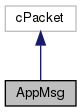
\includegraphics[width=133pt]{class_app_msg__inherit__graph}
\end{center}
\end{figure}


Collaboration diagram for App\+Msg\+:
\nopagebreak
\begin{figure}[H]
\begin{center}
\leavevmode
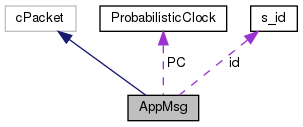
\includegraphics[width=299pt]{class_app_msg__coll__graph}
\end{center}
\end{figure}
\subsection*{Public Member Functions}
\begin{DoxyCompactItemize}
\item 
\hyperlink{class_app_msg_abcde1b0a82cb815e59b04ba891f8d1a0}{App\+Msg} (const char $\ast$name=nullptr, short kind=0)
\item 
\hyperlink{class_app_msg_a1b1df77f37c0aba71d69dd65b963c5d5}{App\+Msg} (const \hyperlink{class_app_msg}{App\+Msg} \&other)
\item 
virtual \hyperlink{class_app_msg_ac15790acabb2755dd83d1d29f57e498c}{$\sim$\+App\+Msg} ()
\item 
\hyperlink{class_app_msg}{App\+Msg} \& \hyperlink{class_app_msg_abb8f6f1fa21e6597ff28f6df72b435ad}{operator=} (const \hyperlink{class_app_msg}{App\+Msg} \&other)
\item 
virtual \hyperlink{class_app_msg}{App\+Msg} $\ast$ \hyperlink{class_app_msg_ab4d1256f22c1ee48aec128e558a03940}{dup} () const override
\item 
virtual void \hyperlink{class_app_msg_a97036583c6a13015d1be1ac6cf87505e}{parsim\+Pack} (omnetpp\+::c\+Comm\+Buffer $\ast$b) const override
\item 
virtual void \hyperlink{class_app_msg_a6852bb25218542149dcfb9f8ba672b7f}{parsim\+Unpack} (omnetpp\+::c\+Comm\+Buffer $\ast$b) override
\item 
virtual \hyperlink{_app_msg__m_8h_a0bd5e3a5ba85ac1fa0fd0fae34d903c1}{id\+Msg\+App\+Msg} \& \hyperlink{class_app_msg_abd9e4fa4ce0b074123b4e0cf64f5d743}{get\+Id} ()
\item 
virtual const \hyperlink{_app_msg__m_8h_a0bd5e3a5ba85ac1fa0fd0fae34d903c1}{id\+Msg\+App\+Msg} \& \hyperlink{class_app_msg_a0a87f5d332044dcd5ce861f6bcfaf6b2}{get\+Id} () const
\item 
virtual void \hyperlink{class_app_msg_ac76f921f7a873b5ca4b944fbbacfdf1c}{set\+Id} (const \hyperlink{_app_msg__m_8h_a0bd5e3a5ba85ac1fa0fd0fae34d903c1}{id\+Msg\+App\+Msg} \&\hyperlink{class_app_msg_aadaa93732c4df84c8b2ef13d7199f9a1}{id})
\item 
virtual \hyperlink{_app_msg__m_8h_abcd76636e4b750d033ffc348601dd7a2}{App\+Msg\+PC} \& \hyperlink{class_app_msg_a50acdb9331a812120c945612e81cd04f}{get\+PC} ()
\item 
virtual const \hyperlink{_app_msg__m_8h_abcd76636e4b750d033ffc348601dd7a2}{App\+Msg\+PC} \& \hyperlink{class_app_msg_a19864419107e294ac7c64553ceb5a9f0}{get\+PC} () const
\item 
virtual void \hyperlink{class_app_msg_a36ed2ccb047c20c26292687c44acd79b}{set\+PC} (const \hyperlink{_app_msg__m_8h_abcd76636e4b750d033ffc348601dd7a2}{App\+Msg\+PC} \&\hyperlink{class_app_msg_a0dceb6642736a90673422df92ab3d788}{PC})
\item 
virtual unsigned long \hyperlink{class_app_msg_a59f818e49bf28c2fd494e6668ef13367}{get\+Hash} () const
\item 
virtual void \hyperlink{class_app_msg_afd406d5bf0b92892a1ebf8fe3397331a}{set\+Hash} (unsigned long \hyperlink{class_app_msg_a8b73e331d42d97d9e51603dc5352307f}{hash})
\item 
virtual \hyperlink{_app_msg__m_8h_afd955b091e7d9b98cff80a090db1eb09}{App\+Msg\+Time} \& \hyperlink{class_app_msg_aa45e97cdd014921d271665e856c642cc}{get\+Delay} ()
\item 
virtual const \hyperlink{_app_msg__m_8h_afd955b091e7d9b98cff80a090db1eb09}{App\+Msg\+Time} \& \hyperlink{class_app_msg_ac735d5e96a9c7fe0281d617820d7b533}{get\+Delay} () const
\item 
virtual void \hyperlink{class_app_msg_a81ed720c6233e90a97ab0dd928be6574}{set\+Delay} (const \hyperlink{_app_msg__m_8h_afd955b091e7d9b98cff80a090db1eb09}{App\+Msg\+Time} \&\hyperlink{class_app_msg_af7a10648a9051ad068c0b2660c7bb545}{delay})
\item 
virtual \hyperlink{_app_msg__m_8h_a2b8cadfd13c916ddccf5a213ca34d8ee}{App\+Msg\+False\+Dep} \& \hyperlink{class_app_msg_a0578104e6c8983ba88270192b263e3c9}{get\+False\+Dependencies} ()
\item 
virtual const \hyperlink{_app_msg__m_8h_a2b8cadfd13c916ddccf5a213ca34d8ee}{App\+Msg\+False\+Dep} \& \hyperlink{class_app_msg_aa9c4237b7fafc07ee9ba6d798941cc06}{get\+False\+Dependencies} () const
\item 
virtual void \hyperlink{class_app_msg_ab810112cdc978f6c93b2d45e4aa6f094}{set\+False\+Dependencies} (const \hyperlink{_app_msg__m_8h_a2b8cadfd13c916ddccf5a213ca34d8ee}{App\+Msg\+False\+Dep} \&\hyperlink{class_app_msg_a2e1c93236ae4ceb0fc5571a5b044c454}{false\+Dependencies})
\item 
virtual \hyperlink{_app_msg__m_8h_a39bb58326d7e24febcd7397c022ada6a}{App\+Msg\+Dep} \& \hyperlink{class_app_msg_ae767d2a50a7b279bdecf457fd047125a}{get\+Dependencies} ()
\item 
virtual const \hyperlink{_app_msg__m_8h_a39bb58326d7e24febcd7397c022ada6a}{App\+Msg\+Dep} \& \hyperlink{class_app_msg_a453ca3d6502f7f82020c7ef2787a45c7}{get\+Dependencies} () const
\item 
virtual void \hyperlink{class_app_msg_a1f648f7d16c4f3329fffb6b4e73e969c}{set\+Dependencies} (const \hyperlink{_app_msg__m_8h_a39bb58326d7e24febcd7397c022ada6a}{App\+Msg\+Dep} \&\hyperlink{class_app_msg_a6f78bb134b9a39321ad8093da19d8c8b}{dependencies})
\end{DoxyCompactItemize}
\subsection*{Protected Member Functions}
\begin{DoxyCompactItemize}
\item 
bool \hyperlink{class_app_msg_a5eb13ac34b1364ca33dbf8f563b9e81c}{operator==} (const \hyperlink{class_app_msg}{App\+Msg} \&)
\end{DoxyCompactItemize}
\subsection*{Protected Attributes}
\begin{DoxyCompactItemize}
\item 
\hyperlink{_app_msg__m_8h_a0bd5e3a5ba85ac1fa0fd0fae34d903c1}{id\+Msg\+App\+Msg} \hyperlink{class_app_msg_aadaa93732c4df84c8b2ef13d7199f9a1}{id}
\item 
\hyperlink{_app_msg__m_8h_abcd76636e4b750d033ffc348601dd7a2}{App\+Msg\+PC} \hyperlink{class_app_msg_a0dceb6642736a90673422df92ab3d788}{PC}
\item 
unsigned long \hyperlink{class_app_msg_a8b73e331d42d97d9e51603dc5352307f}{hash}
\item 
\hyperlink{_app_msg__m_8h_afd955b091e7d9b98cff80a090db1eb09}{App\+Msg\+Time} \hyperlink{class_app_msg_af7a10648a9051ad068c0b2660c7bb545}{delay}
\item 
\hyperlink{_app_msg__m_8h_a2b8cadfd13c916ddccf5a213ca34d8ee}{App\+Msg\+False\+Dep} \hyperlink{class_app_msg_a2e1c93236ae4ceb0fc5571a5b044c454}{false\+Dependencies}
\item 
\hyperlink{_app_msg__m_8h_a39bb58326d7e24febcd7397c022ada6a}{App\+Msg\+Dep} \hyperlink{class_app_msg_a6f78bb134b9a39321ad8093da19d8c8b}{dependencies}
\end{DoxyCompactItemize}
\subsection*{Private Member Functions}
\begin{DoxyCompactItemize}
\item 
void \hyperlink{class_app_msg_a2d5c5dacc13f5e7959467693cd0beda9}{copy} (const \hyperlink{class_app_msg}{App\+Msg} \&other)
\end{DoxyCompactItemize}


\subsection{Detailed Description}
Class generated from {\ttfamily Messages/\+App\+Msg.\+msg\+:48} by nedtool. 


\begin{DoxyPre}
packet \hyperlink{class_app_msg}{AppMsg}
\{
    idMsgAppMsg id;
    AppMsgPC PC;
    unsigned long hash;
    AppMsgTime delay; // ms 
    AppMsgFalseDep falseDependencies;
    AppMsgDep dependencies;
\}
\end{DoxyPre}
 

\subsection{Constructor \& Destructor Documentation}
\mbox{\Hypertarget{class_app_msg_abcde1b0a82cb815e59b04ba891f8d1a0}\label{class_app_msg_abcde1b0a82cb815e59b04ba891f8d1a0}} 
\index{App\+Msg@{App\+Msg}!App\+Msg@{App\+Msg}}
\index{App\+Msg@{App\+Msg}!App\+Msg@{App\+Msg}}
\subsubsection{\texorpdfstring{App\+Msg()}{AppMsg()}\hspace{0.1cm}{\footnotesize\ttfamily [1/2]}}
{\footnotesize\ttfamily App\+Msg\+::\+App\+Msg (\begin{DoxyParamCaption}\item[{const char $\ast$}]{name = {\ttfamily nullptr},  }\item[{short}]{kind = {\ttfamily 0} }\end{DoxyParamCaption})}

\mbox{\Hypertarget{class_app_msg_a1b1df77f37c0aba71d69dd65b963c5d5}\label{class_app_msg_a1b1df77f37c0aba71d69dd65b963c5d5}} 
\index{App\+Msg@{App\+Msg}!App\+Msg@{App\+Msg}}
\index{App\+Msg@{App\+Msg}!App\+Msg@{App\+Msg}}
\subsubsection{\texorpdfstring{App\+Msg()}{AppMsg()}\hspace{0.1cm}{\footnotesize\ttfamily [2/2]}}
{\footnotesize\ttfamily App\+Msg\+::\+App\+Msg (\begin{DoxyParamCaption}\item[{const \hyperlink{class_app_msg}{App\+Msg} \&}]{other }\end{DoxyParamCaption})}

\mbox{\Hypertarget{class_app_msg_ac15790acabb2755dd83d1d29f57e498c}\label{class_app_msg_ac15790acabb2755dd83d1d29f57e498c}} 
\index{App\+Msg@{App\+Msg}!````~App\+Msg@{$\sim$\+App\+Msg}}
\index{````~App\+Msg@{$\sim$\+App\+Msg}!App\+Msg@{App\+Msg}}
\subsubsection{\texorpdfstring{$\sim$\+App\+Msg()}{~AppMsg()}}
{\footnotesize\ttfamily App\+Msg\+::$\sim$\+App\+Msg (\begin{DoxyParamCaption}{ }\end{DoxyParamCaption})\hspace{0.3cm}{\ttfamily [virtual]}}



\subsection{Member Function Documentation}
\mbox{\Hypertarget{class_app_msg_a2d5c5dacc13f5e7959467693cd0beda9}\label{class_app_msg_a2d5c5dacc13f5e7959467693cd0beda9}} 
\index{App\+Msg@{App\+Msg}!copy@{copy}}
\index{copy@{copy}!App\+Msg@{App\+Msg}}
\subsubsection{\texorpdfstring{copy()}{copy()}}
{\footnotesize\ttfamily void App\+Msg\+::copy (\begin{DoxyParamCaption}\item[{const \hyperlink{class_app_msg}{App\+Msg} \&}]{other }\end{DoxyParamCaption})\hspace{0.3cm}{\ttfamily [private]}}

\mbox{\Hypertarget{class_app_msg_ab4d1256f22c1ee48aec128e558a03940}\label{class_app_msg_ab4d1256f22c1ee48aec128e558a03940}} 
\index{App\+Msg@{App\+Msg}!dup@{dup}}
\index{dup@{dup}!App\+Msg@{App\+Msg}}
\subsubsection{\texorpdfstring{dup()}{dup()}}
{\footnotesize\ttfamily virtual \hyperlink{class_app_msg}{App\+Msg}$\ast$ App\+Msg\+::dup (\begin{DoxyParamCaption}{ }\end{DoxyParamCaption}) const\hspace{0.3cm}{\ttfamily [inline]}, {\ttfamily [override]}, {\ttfamily [virtual]}}

\mbox{\Hypertarget{class_app_msg_aa45e97cdd014921d271665e856c642cc}\label{class_app_msg_aa45e97cdd014921d271665e856c642cc}} 
\index{App\+Msg@{App\+Msg}!get\+Delay@{get\+Delay}}
\index{get\+Delay@{get\+Delay}!App\+Msg@{App\+Msg}}
\subsubsection{\texorpdfstring{get\+Delay()}{getDelay()}\hspace{0.1cm}{\footnotesize\ttfamily [1/2]}}
{\footnotesize\ttfamily \hyperlink{_app_msg__m_8h_afd955b091e7d9b98cff80a090db1eb09}{App\+Msg\+Time} \& App\+Msg\+::get\+Delay (\begin{DoxyParamCaption}{ }\end{DoxyParamCaption})\hspace{0.3cm}{\ttfamily [virtual]}}

\mbox{\Hypertarget{class_app_msg_ac735d5e96a9c7fe0281d617820d7b533}\label{class_app_msg_ac735d5e96a9c7fe0281d617820d7b533}} 
\index{App\+Msg@{App\+Msg}!get\+Delay@{get\+Delay}}
\index{get\+Delay@{get\+Delay}!App\+Msg@{App\+Msg}}
\subsubsection{\texorpdfstring{get\+Delay()}{getDelay()}\hspace{0.1cm}{\footnotesize\ttfamily [2/2]}}
{\footnotesize\ttfamily virtual const \hyperlink{_app_msg__m_8h_afd955b091e7d9b98cff80a090db1eb09}{App\+Msg\+Time}\& App\+Msg\+::get\+Delay (\begin{DoxyParamCaption}{ }\end{DoxyParamCaption}) const\hspace{0.3cm}{\ttfamily [inline]}, {\ttfamily [virtual]}}

\mbox{\Hypertarget{class_app_msg_ae767d2a50a7b279bdecf457fd047125a}\label{class_app_msg_ae767d2a50a7b279bdecf457fd047125a}} 
\index{App\+Msg@{App\+Msg}!get\+Dependencies@{get\+Dependencies}}
\index{get\+Dependencies@{get\+Dependencies}!App\+Msg@{App\+Msg}}
\subsubsection{\texorpdfstring{get\+Dependencies()}{getDependencies()}\hspace{0.1cm}{\footnotesize\ttfamily [1/2]}}
{\footnotesize\ttfamily \hyperlink{_app_msg__m_8h_a39bb58326d7e24febcd7397c022ada6a}{App\+Msg\+Dep} \& App\+Msg\+::get\+Dependencies (\begin{DoxyParamCaption}{ }\end{DoxyParamCaption})\hspace{0.3cm}{\ttfamily [virtual]}}

\mbox{\Hypertarget{class_app_msg_a453ca3d6502f7f82020c7ef2787a45c7}\label{class_app_msg_a453ca3d6502f7f82020c7ef2787a45c7}} 
\index{App\+Msg@{App\+Msg}!get\+Dependencies@{get\+Dependencies}}
\index{get\+Dependencies@{get\+Dependencies}!App\+Msg@{App\+Msg}}
\subsubsection{\texorpdfstring{get\+Dependencies()}{getDependencies()}\hspace{0.1cm}{\footnotesize\ttfamily [2/2]}}
{\footnotesize\ttfamily virtual const \hyperlink{_app_msg__m_8h_a39bb58326d7e24febcd7397c022ada6a}{App\+Msg\+Dep}\& App\+Msg\+::get\+Dependencies (\begin{DoxyParamCaption}{ }\end{DoxyParamCaption}) const\hspace{0.3cm}{\ttfamily [inline]}, {\ttfamily [virtual]}}

\mbox{\Hypertarget{class_app_msg_a0578104e6c8983ba88270192b263e3c9}\label{class_app_msg_a0578104e6c8983ba88270192b263e3c9}} 
\index{App\+Msg@{App\+Msg}!get\+False\+Dependencies@{get\+False\+Dependencies}}
\index{get\+False\+Dependencies@{get\+False\+Dependencies}!App\+Msg@{App\+Msg}}
\subsubsection{\texorpdfstring{get\+False\+Dependencies()}{getFalseDependencies()}\hspace{0.1cm}{\footnotesize\ttfamily [1/2]}}
{\footnotesize\ttfamily \hyperlink{_app_msg__m_8h_a2b8cadfd13c916ddccf5a213ca34d8ee}{App\+Msg\+False\+Dep} \& App\+Msg\+::get\+False\+Dependencies (\begin{DoxyParamCaption}{ }\end{DoxyParamCaption})\hspace{0.3cm}{\ttfamily [virtual]}}

\mbox{\Hypertarget{class_app_msg_aa9c4237b7fafc07ee9ba6d798941cc06}\label{class_app_msg_aa9c4237b7fafc07ee9ba6d798941cc06}} 
\index{App\+Msg@{App\+Msg}!get\+False\+Dependencies@{get\+False\+Dependencies}}
\index{get\+False\+Dependencies@{get\+False\+Dependencies}!App\+Msg@{App\+Msg}}
\subsubsection{\texorpdfstring{get\+False\+Dependencies()}{getFalseDependencies()}\hspace{0.1cm}{\footnotesize\ttfamily [2/2]}}
{\footnotesize\ttfamily virtual const \hyperlink{_app_msg__m_8h_a2b8cadfd13c916ddccf5a213ca34d8ee}{App\+Msg\+False\+Dep}\& App\+Msg\+::get\+False\+Dependencies (\begin{DoxyParamCaption}{ }\end{DoxyParamCaption}) const\hspace{0.3cm}{\ttfamily [inline]}, {\ttfamily [virtual]}}

\mbox{\Hypertarget{class_app_msg_a59f818e49bf28c2fd494e6668ef13367}\label{class_app_msg_a59f818e49bf28c2fd494e6668ef13367}} 
\index{App\+Msg@{App\+Msg}!get\+Hash@{get\+Hash}}
\index{get\+Hash@{get\+Hash}!App\+Msg@{App\+Msg}}
\subsubsection{\texorpdfstring{get\+Hash()}{getHash()}}
{\footnotesize\ttfamily unsigned long App\+Msg\+::get\+Hash (\begin{DoxyParamCaption}{ }\end{DoxyParamCaption}) const\hspace{0.3cm}{\ttfamily [virtual]}}

\mbox{\Hypertarget{class_app_msg_abd9e4fa4ce0b074123b4e0cf64f5d743}\label{class_app_msg_abd9e4fa4ce0b074123b4e0cf64f5d743}} 
\index{App\+Msg@{App\+Msg}!get\+Id@{get\+Id}}
\index{get\+Id@{get\+Id}!App\+Msg@{App\+Msg}}
\subsubsection{\texorpdfstring{get\+Id()}{getId()}\hspace{0.1cm}{\footnotesize\ttfamily [1/2]}}
{\footnotesize\ttfamily \hyperlink{_app_msg__m_8h_a0bd5e3a5ba85ac1fa0fd0fae34d903c1}{id\+Msg\+App\+Msg} \& App\+Msg\+::get\+Id (\begin{DoxyParamCaption}{ }\end{DoxyParamCaption})\hspace{0.3cm}{\ttfamily [virtual]}}

\mbox{\Hypertarget{class_app_msg_a0a87f5d332044dcd5ce861f6bcfaf6b2}\label{class_app_msg_a0a87f5d332044dcd5ce861f6bcfaf6b2}} 
\index{App\+Msg@{App\+Msg}!get\+Id@{get\+Id}}
\index{get\+Id@{get\+Id}!App\+Msg@{App\+Msg}}
\subsubsection{\texorpdfstring{get\+Id()}{getId()}\hspace{0.1cm}{\footnotesize\ttfamily [2/2]}}
{\footnotesize\ttfamily virtual const \hyperlink{_app_msg__m_8h_a0bd5e3a5ba85ac1fa0fd0fae34d903c1}{id\+Msg\+App\+Msg}\& App\+Msg\+::get\+Id (\begin{DoxyParamCaption}{ }\end{DoxyParamCaption}) const\hspace{0.3cm}{\ttfamily [inline]}, {\ttfamily [virtual]}}

\mbox{\Hypertarget{class_app_msg_a50acdb9331a812120c945612e81cd04f}\label{class_app_msg_a50acdb9331a812120c945612e81cd04f}} 
\index{App\+Msg@{App\+Msg}!get\+PC@{get\+PC}}
\index{get\+PC@{get\+PC}!App\+Msg@{App\+Msg}}
\subsubsection{\texorpdfstring{get\+P\+C()}{getPC()}\hspace{0.1cm}{\footnotesize\ttfamily [1/2]}}
{\footnotesize\ttfamily \hyperlink{_app_msg__m_8h_abcd76636e4b750d033ffc348601dd7a2}{App\+Msg\+PC} \& App\+Msg\+::get\+PC (\begin{DoxyParamCaption}{ }\end{DoxyParamCaption})\hspace{0.3cm}{\ttfamily [virtual]}}

\mbox{\Hypertarget{class_app_msg_a19864419107e294ac7c64553ceb5a9f0}\label{class_app_msg_a19864419107e294ac7c64553ceb5a9f0}} 
\index{App\+Msg@{App\+Msg}!get\+PC@{get\+PC}}
\index{get\+PC@{get\+PC}!App\+Msg@{App\+Msg}}
\subsubsection{\texorpdfstring{get\+P\+C()}{getPC()}\hspace{0.1cm}{\footnotesize\ttfamily [2/2]}}
{\footnotesize\ttfamily virtual const \hyperlink{_app_msg__m_8h_abcd76636e4b750d033ffc348601dd7a2}{App\+Msg\+PC}\& App\+Msg\+::get\+PC (\begin{DoxyParamCaption}{ }\end{DoxyParamCaption}) const\hspace{0.3cm}{\ttfamily [inline]}, {\ttfamily [virtual]}}

\mbox{\Hypertarget{class_app_msg_abb8f6f1fa21e6597ff28f6df72b435ad}\label{class_app_msg_abb8f6f1fa21e6597ff28f6df72b435ad}} 
\index{App\+Msg@{App\+Msg}!operator=@{operator=}}
\index{operator=@{operator=}!App\+Msg@{App\+Msg}}
\subsubsection{\texorpdfstring{operator=()}{operator=()}}
{\footnotesize\ttfamily \hyperlink{class_app_msg}{App\+Msg} \& App\+Msg\+::operator= (\begin{DoxyParamCaption}\item[{const \hyperlink{class_app_msg}{App\+Msg} \&}]{other }\end{DoxyParamCaption})}

\mbox{\Hypertarget{class_app_msg_a5eb13ac34b1364ca33dbf8f563b9e81c}\label{class_app_msg_a5eb13ac34b1364ca33dbf8f563b9e81c}} 
\index{App\+Msg@{App\+Msg}!operator==@{operator==}}
\index{operator==@{operator==}!App\+Msg@{App\+Msg}}
\subsubsection{\texorpdfstring{operator==()}{operator==()}}
{\footnotesize\ttfamily bool App\+Msg\+::operator== (\begin{DoxyParamCaption}\item[{const \hyperlink{class_app_msg}{App\+Msg} \&}]{ }\end{DoxyParamCaption})\hspace{0.3cm}{\ttfamily [protected]}}

\mbox{\Hypertarget{class_app_msg_a97036583c6a13015d1be1ac6cf87505e}\label{class_app_msg_a97036583c6a13015d1be1ac6cf87505e}} 
\index{App\+Msg@{App\+Msg}!parsim\+Pack@{parsim\+Pack}}
\index{parsim\+Pack@{parsim\+Pack}!App\+Msg@{App\+Msg}}
\subsubsection{\texorpdfstring{parsim\+Pack()}{parsimPack()}}
{\footnotesize\ttfamily void App\+Msg\+::parsim\+Pack (\begin{DoxyParamCaption}\item[{omnetpp\+::c\+Comm\+Buffer $\ast$}]{b }\end{DoxyParamCaption}) const\hspace{0.3cm}{\ttfamily [override]}, {\ttfamily [virtual]}}

\mbox{\Hypertarget{class_app_msg_a6852bb25218542149dcfb9f8ba672b7f}\label{class_app_msg_a6852bb25218542149dcfb9f8ba672b7f}} 
\index{App\+Msg@{App\+Msg}!parsim\+Unpack@{parsim\+Unpack}}
\index{parsim\+Unpack@{parsim\+Unpack}!App\+Msg@{App\+Msg}}
\subsubsection{\texorpdfstring{parsim\+Unpack()}{parsimUnpack()}}
{\footnotesize\ttfamily void App\+Msg\+::parsim\+Unpack (\begin{DoxyParamCaption}\item[{omnetpp\+::c\+Comm\+Buffer $\ast$}]{b }\end{DoxyParamCaption})\hspace{0.3cm}{\ttfamily [override]}, {\ttfamily [virtual]}}

\mbox{\Hypertarget{class_app_msg_a81ed720c6233e90a97ab0dd928be6574}\label{class_app_msg_a81ed720c6233e90a97ab0dd928be6574}} 
\index{App\+Msg@{App\+Msg}!set\+Delay@{set\+Delay}}
\index{set\+Delay@{set\+Delay}!App\+Msg@{App\+Msg}}
\subsubsection{\texorpdfstring{set\+Delay()}{setDelay()}}
{\footnotesize\ttfamily void App\+Msg\+::set\+Delay (\begin{DoxyParamCaption}\item[{const \hyperlink{_app_msg__m_8h_afd955b091e7d9b98cff80a090db1eb09}{App\+Msg\+Time} \&}]{delay }\end{DoxyParamCaption})\hspace{0.3cm}{\ttfamily [virtual]}}

\mbox{\Hypertarget{class_app_msg_a1f648f7d16c4f3329fffb6b4e73e969c}\label{class_app_msg_a1f648f7d16c4f3329fffb6b4e73e969c}} 
\index{App\+Msg@{App\+Msg}!set\+Dependencies@{set\+Dependencies}}
\index{set\+Dependencies@{set\+Dependencies}!App\+Msg@{App\+Msg}}
\subsubsection{\texorpdfstring{set\+Dependencies()}{setDependencies()}}
{\footnotesize\ttfamily void App\+Msg\+::set\+Dependencies (\begin{DoxyParamCaption}\item[{const \hyperlink{_app_msg__m_8h_a39bb58326d7e24febcd7397c022ada6a}{App\+Msg\+Dep} \&}]{dependencies }\end{DoxyParamCaption})\hspace{0.3cm}{\ttfamily [virtual]}}

\mbox{\Hypertarget{class_app_msg_ab810112cdc978f6c93b2d45e4aa6f094}\label{class_app_msg_ab810112cdc978f6c93b2d45e4aa6f094}} 
\index{App\+Msg@{App\+Msg}!set\+False\+Dependencies@{set\+False\+Dependencies}}
\index{set\+False\+Dependencies@{set\+False\+Dependencies}!App\+Msg@{App\+Msg}}
\subsubsection{\texorpdfstring{set\+False\+Dependencies()}{setFalseDependencies()}}
{\footnotesize\ttfamily void App\+Msg\+::set\+False\+Dependencies (\begin{DoxyParamCaption}\item[{const \hyperlink{_app_msg__m_8h_a2b8cadfd13c916ddccf5a213ca34d8ee}{App\+Msg\+False\+Dep} \&}]{false\+Dependencies }\end{DoxyParamCaption})\hspace{0.3cm}{\ttfamily [virtual]}}

\mbox{\Hypertarget{class_app_msg_afd406d5bf0b92892a1ebf8fe3397331a}\label{class_app_msg_afd406d5bf0b92892a1ebf8fe3397331a}} 
\index{App\+Msg@{App\+Msg}!set\+Hash@{set\+Hash}}
\index{set\+Hash@{set\+Hash}!App\+Msg@{App\+Msg}}
\subsubsection{\texorpdfstring{set\+Hash()}{setHash()}}
{\footnotesize\ttfamily void App\+Msg\+::set\+Hash (\begin{DoxyParamCaption}\item[{unsigned long}]{hash }\end{DoxyParamCaption})\hspace{0.3cm}{\ttfamily [virtual]}}

\mbox{\Hypertarget{class_app_msg_ac76f921f7a873b5ca4b944fbbacfdf1c}\label{class_app_msg_ac76f921f7a873b5ca4b944fbbacfdf1c}} 
\index{App\+Msg@{App\+Msg}!set\+Id@{set\+Id}}
\index{set\+Id@{set\+Id}!App\+Msg@{App\+Msg}}
\subsubsection{\texorpdfstring{set\+Id()}{setId()}}
{\footnotesize\ttfamily void App\+Msg\+::set\+Id (\begin{DoxyParamCaption}\item[{const \hyperlink{_app_msg__m_8h_a0bd5e3a5ba85ac1fa0fd0fae34d903c1}{id\+Msg\+App\+Msg} \&}]{id }\end{DoxyParamCaption})\hspace{0.3cm}{\ttfamily [virtual]}}

\mbox{\Hypertarget{class_app_msg_a36ed2ccb047c20c26292687c44acd79b}\label{class_app_msg_a36ed2ccb047c20c26292687c44acd79b}} 
\index{App\+Msg@{App\+Msg}!set\+PC@{set\+PC}}
\index{set\+PC@{set\+PC}!App\+Msg@{App\+Msg}}
\subsubsection{\texorpdfstring{set\+P\+C()}{setPC()}}
{\footnotesize\ttfamily void App\+Msg\+::set\+PC (\begin{DoxyParamCaption}\item[{const \hyperlink{_app_msg__m_8h_abcd76636e4b750d033ffc348601dd7a2}{App\+Msg\+PC} \&}]{PC }\end{DoxyParamCaption})\hspace{0.3cm}{\ttfamily [virtual]}}



\subsection{Member Data Documentation}
\mbox{\Hypertarget{class_app_msg_af7a10648a9051ad068c0b2660c7bb545}\label{class_app_msg_af7a10648a9051ad068c0b2660c7bb545}} 
\index{App\+Msg@{App\+Msg}!delay@{delay}}
\index{delay@{delay}!App\+Msg@{App\+Msg}}
\subsubsection{\texorpdfstring{delay}{delay}}
{\footnotesize\ttfamily \hyperlink{_app_msg__m_8h_afd955b091e7d9b98cff80a090db1eb09}{App\+Msg\+Time} App\+Msg\+::delay\hspace{0.3cm}{\ttfamily [protected]}}

\mbox{\Hypertarget{class_app_msg_a6f78bb134b9a39321ad8093da19d8c8b}\label{class_app_msg_a6f78bb134b9a39321ad8093da19d8c8b}} 
\index{App\+Msg@{App\+Msg}!dependencies@{dependencies}}
\index{dependencies@{dependencies}!App\+Msg@{App\+Msg}}
\subsubsection{\texorpdfstring{dependencies}{dependencies}}
{\footnotesize\ttfamily \hyperlink{_app_msg__m_8h_a39bb58326d7e24febcd7397c022ada6a}{App\+Msg\+Dep} App\+Msg\+::dependencies\hspace{0.3cm}{\ttfamily [protected]}}

\mbox{\Hypertarget{class_app_msg_a2e1c93236ae4ceb0fc5571a5b044c454}\label{class_app_msg_a2e1c93236ae4ceb0fc5571a5b044c454}} 
\index{App\+Msg@{App\+Msg}!false\+Dependencies@{false\+Dependencies}}
\index{false\+Dependencies@{false\+Dependencies}!App\+Msg@{App\+Msg}}
\subsubsection{\texorpdfstring{false\+Dependencies}{falseDependencies}}
{\footnotesize\ttfamily \hyperlink{_app_msg__m_8h_a2b8cadfd13c916ddccf5a213ca34d8ee}{App\+Msg\+False\+Dep} App\+Msg\+::false\+Dependencies\hspace{0.3cm}{\ttfamily [protected]}}

\mbox{\Hypertarget{class_app_msg_a8b73e331d42d97d9e51603dc5352307f}\label{class_app_msg_a8b73e331d42d97d9e51603dc5352307f}} 
\index{App\+Msg@{App\+Msg}!hash@{hash}}
\index{hash@{hash}!App\+Msg@{App\+Msg}}
\subsubsection{\texorpdfstring{hash}{hash}}
{\footnotesize\ttfamily unsigned long App\+Msg\+::hash\hspace{0.3cm}{\ttfamily [protected]}}

\mbox{\Hypertarget{class_app_msg_aadaa93732c4df84c8b2ef13d7199f9a1}\label{class_app_msg_aadaa93732c4df84c8b2ef13d7199f9a1}} 
\index{App\+Msg@{App\+Msg}!id@{id}}
\index{id@{id}!App\+Msg@{App\+Msg}}
\subsubsection{\texorpdfstring{id}{id}}
{\footnotesize\ttfamily \hyperlink{_app_msg__m_8h_a0bd5e3a5ba85ac1fa0fd0fae34d903c1}{id\+Msg\+App\+Msg} App\+Msg\+::id\hspace{0.3cm}{\ttfamily [protected]}}

\mbox{\Hypertarget{class_app_msg_a0dceb6642736a90673422df92ab3d788}\label{class_app_msg_a0dceb6642736a90673422df92ab3d788}} 
\index{App\+Msg@{App\+Msg}!PC@{PC}}
\index{PC@{PC}!App\+Msg@{App\+Msg}}
\subsubsection{\texorpdfstring{PC}{PC}}
{\footnotesize\ttfamily \hyperlink{_app_msg__m_8h_abcd76636e4b750d033ffc348601dd7a2}{App\+Msg\+PC} App\+Msg\+::\+PC\hspace{0.3cm}{\ttfamily [protected]}}



The documentation for this class was generated from the following files\+:\begin{DoxyCompactItemize}
\item 
/home/wilhelm/\+Documents/code\+Git\+Hub/\+Error\+Detectors/src/\+Messages/\hyperlink{_app_msg__m_8h}{App\+Msg\+\_\+m.\+h}\item 
/home/wilhelm/\+Documents/code\+Git\+Hub/\+Error\+Detectors/src/\+Messages/\hyperlink{_app_msg__m_8cc}{App\+Msg\+\_\+m.\+cc}\end{DoxyCompactItemize}

\hypertarget{class_app_msg_dep_descriptor}{}\section{App\+Msg\+Dep\+Descriptor Class Reference}
\label{class_app_msg_dep_descriptor}\index{App\+Msg\+Dep\+Descriptor@{App\+Msg\+Dep\+Descriptor}}


Inheritance diagram for App\+Msg\+Dep\+Descriptor\+:
\nopagebreak
\begin{figure}[H]
\begin{center}
\leavevmode
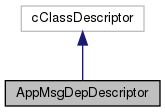
\includegraphics[width=196pt]{class_app_msg_dep_descriptor__inherit__graph}
\end{center}
\end{figure}


Collaboration diagram for App\+Msg\+Dep\+Descriptor\+:
\nopagebreak
\begin{figure}[H]
\begin{center}
\leavevmode
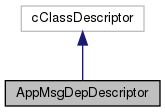
\includegraphics[width=196pt]{class_app_msg_dep_descriptor__coll__graph}
\end{center}
\end{figure}
\subsection*{Public Member Functions}
\begin{DoxyCompactItemize}
\item 
\hyperlink{class_app_msg_dep_descriptor_a9e34bc0dc8c5ebf87d3861c741a1ee78}{App\+Msg\+Dep\+Descriptor} ()
\item 
virtual \hyperlink{class_app_msg_dep_descriptor_aef6f0e8734bc696c3e76065a642ae84e}{$\sim$\+App\+Msg\+Dep\+Descriptor} ()
\item 
virtual bool \hyperlink{class_app_msg_dep_descriptor_ab9ca1804536d49681d6e681f97627c92}{does\+Support} (omnetpp\+::c\+Object $\ast$obj) const override
\item 
virtual const char $\ast$$\ast$ \hyperlink{class_app_msg_dep_descriptor_a52285a3c2457062bf24e71a1b68e266d}{get\+Property\+Names} () const override
\item 
virtual const char $\ast$ \hyperlink{class_app_msg_dep_descriptor_a35837c5cdbb09afde09b6cc89618899e}{get\+Property} (const char $\ast$propertyname) const override
\item 
virtual int \hyperlink{class_app_msg_dep_descriptor_ad204cc9df6c39c659db4382d44bb5138}{get\+Field\+Count} () const override
\item 
virtual const char $\ast$ \hyperlink{class_app_msg_dep_descriptor_abc7c71b322dd44e9e013d796a1847f98}{get\+Field\+Name} (int field) const override
\item 
virtual int \hyperlink{class_app_msg_dep_descriptor_aa3197b479875191ad8c565907640832f}{find\+Field} (const char $\ast$field\+Name) const override
\item 
virtual unsigned int \hyperlink{class_app_msg_dep_descriptor_a14d73b922bf64e60d2401cc2f42acc32}{get\+Field\+Type\+Flags} (int field) const override
\item 
virtual const char $\ast$ \hyperlink{class_app_msg_dep_descriptor_a376972c07aabb5b32e12a38649a56aaf}{get\+Field\+Type\+String} (int field) const override
\item 
virtual const char $\ast$$\ast$ \hyperlink{class_app_msg_dep_descriptor_a2b0c9bca08ff82a4d8bcedf97376a930}{get\+Field\+Property\+Names} (int field) const override
\item 
virtual const char $\ast$ \hyperlink{class_app_msg_dep_descriptor_a5924764c36dbe1f3af75201a843649b6}{get\+Field\+Property} (int field, const char $\ast$propertyname) const override
\item 
virtual int \hyperlink{class_app_msg_dep_descriptor_abd6a2a77ab67f6d4e59a83a4608f1a9f}{get\+Field\+Array\+Size} (void $\ast$object, int field) const override
\item 
virtual const char $\ast$ \hyperlink{class_app_msg_dep_descriptor_a4badf7f0895de3039f46149053f19514}{get\+Field\+Dynamic\+Type\+String} (void $\ast$object, int field, int i) const override
\item 
virtual std\+::string \hyperlink{class_app_msg_dep_descriptor_a83fabb429ce26b55eed23aebe202570d}{get\+Field\+Value\+As\+String} (void $\ast$object, int field, int i) const override
\item 
virtual bool \hyperlink{class_app_msg_dep_descriptor_a47b4aaa772796c7ce821ea2ddff18ad1}{set\+Field\+Value\+As\+String} (void $\ast$object, int field, int i, const char $\ast$value) const override
\item 
virtual const char $\ast$ \hyperlink{class_app_msg_dep_descriptor_af2db18f3d30d0d62bbb5238777f8c478}{get\+Field\+Struct\+Name} (int field) const override
\item 
virtual void $\ast$ \hyperlink{class_app_msg_dep_descriptor_ae62715809f588f4f601bf524a6733be0}{get\+Field\+Struct\+Value\+Pointer} (void $\ast$object, int field, int i) const override
\end{DoxyCompactItemize}
\subsection*{Private Attributes}
\begin{DoxyCompactItemize}
\item 
const char $\ast$$\ast$ \hyperlink{class_app_msg_dep_descriptor_a03578bf1418ef896a9abfcded857b728}{propertynames}
\end{DoxyCompactItemize}


\subsection{Constructor \& Destructor Documentation}
\mbox{\Hypertarget{class_app_msg_dep_descriptor_a9e34bc0dc8c5ebf87d3861c741a1ee78}\label{class_app_msg_dep_descriptor_a9e34bc0dc8c5ebf87d3861c741a1ee78}} 
\index{App\+Msg\+Dep\+Descriptor@{App\+Msg\+Dep\+Descriptor}!App\+Msg\+Dep\+Descriptor@{App\+Msg\+Dep\+Descriptor}}
\index{App\+Msg\+Dep\+Descriptor@{App\+Msg\+Dep\+Descriptor}!App\+Msg\+Dep\+Descriptor@{App\+Msg\+Dep\+Descriptor}}
\subsubsection{\texorpdfstring{App\+Msg\+Dep\+Descriptor()}{AppMsgDepDescriptor()}}
{\footnotesize\ttfamily App\+Msg\+Dep\+Descriptor\+::\+App\+Msg\+Dep\+Descriptor (\begin{DoxyParamCaption}{ }\end{DoxyParamCaption})}

\mbox{\Hypertarget{class_app_msg_dep_descriptor_aef6f0e8734bc696c3e76065a642ae84e}\label{class_app_msg_dep_descriptor_aef6f0e8734bc696c3e76065a642ae84e}} 
\index{App\+Msg\+Dep\+Descriptor@{App\+Msg\+Dep\+Descriptor}!````~App\+Msg\+Dep\+Descriptor@{$\sim$\+App\+Msg\+Dep\+Descriptor}}
\index{````~App\+Msg\+Dep\+Descriptor@{$\sim$\+App\+Msg\+Dep\+Descriptor}!App\+Msg\+Dep\+Descriptor@{App\+Msg\+Dep\+Descriptor}}
\subsubsection{\texorpdfstring{$\sim$\+App\+Msg\+Dep\+Descriptor()}{~AppMsgDepDescriptor()}}
{\footnotesize\ttfamily App\+Msg\+Dep\+Descriptor\+::$\sim$\+App\+Msg\+Dep\+Descriptor (\begin{DoxyParamCaption}{ }\end{DoxyParamCaption})\hspace{0.3cm}{\ttfamily [virtual]}}



\subsection{Member Function Documentation}
\mbox{\Hypertarget{class_app_msg_dep_descriptor_ab9ca1804536d49681d6e681f97627c92}\label{class_app_msg_dep_descriptor_ab9ca1804536d49681d6e681f97627c92}} 
\index{App\+Msg\+Dep\+Descriptor@{App\+Msg\+Dep\+Descriptor}!does\+Support@{does\+Support}}
\index{does\+Support@{does\+Support}!App\+Msg\+Dep\+Descriptor@{App\+Msg\+Dep\+Descriptor}}
\subsubsection{\texorpdfstring{does\+Support()}{doesSupport()}}
{\footnotesize\ttfamily bool App\+Msg\+Dep\+Descriptor\+::does\+Support (\begin{DoxyParamCaption}\item[{omnetpp\+::c\+Object $\ast$}]{obj }\end{DoxyParamCaption}) const\hspace{0.3cm}{\ttfamily [override]}, {\ttfamily [virtual]}}

\mbox{\Hypertarget{class_app_msg_dep_descriptor_aa3197b479875191ad8c565907640832f}\label{class_app_msg_dep_descriptor_aa3197b479875191ad8c565907640832f}} 
\index{App\+Msg\+Dep\+Descriptor@{App\+Msg\+Dep\+Descriptor}!find\+Field@{find\+Field}}
\index{find\+Field@{find\+Field}!App\+Msg\+Dep\+Descriptor@{App\+Msg\+Dep\+Descriptor}}
\subsubsection{\texorpdfstring{find\+Field()}{findField()}}
{\footnotesize\ttfamily int App\+Msg\+Dep\+Descriptor\+::find\+Field (\begin{DoxyParamCaption}\item[{const char $\ast$}]{field\+Name }\end{DoxyParamCaption}) const\hspace{0.3cm}{\ttfamily [override]}, {\ttfamily [virtual]}}

\mbox{\Hypertarget{class_app_msg_dep_descriptor_abd6a2a77ab67f6d4e59a83a4608f1a9f}\label{class_app_msg_dep_descriptor_abd6a2a77ab67f6d4e59a83a4608f1a9f}} 
\index{App\+Msg\+Dep\+Descriptor@{App\+Msg\+Dep\+Descriptor}!get\+Field\+Array\+Size@{get\+Field\+Array\+Size}}
\index{get\+Field\+Array\+Size@{get\+Field\+Array\+Size}!App\+Msg\+Dep\+Descriptor@{App\+Msg\+Dep\+Descriptor}}
\subsubsection{\texorpdfstring{get\+Field\+Array\+Size()}{getFieldArraySize()}}
{\footnotesize\ttfamily int App\+Msg\+Dep\+Descriptor\+::get\+Field\+Array\+Size (\begin{DoxyParamCaption}\item[{void $\ast$}]{object,  }\item[{int}]{field }\end{DoxyParamCaption}) const\hspace{0.3cm}{\ttfamily [override]}, {\ttfamily [virtual]}}

\mbox{\Hypertarget{class_app_msg_dep_descriptor_ad204cc9df6c39c659db4382d44bb5138}\label{class_app_msg_dep_descriptor_ad204cc9df6c39c659db4382d44bb5138}} 
\index{App\+Msg\+Dep\+Descriptor@{App\+Msg\+Dep\+Descriptor}!get\+Field\+Count@{get\+Field\+Count}}
\index{get\+Field\+Count@{get\+Field\+Count}!App\+Msg\+Dep\+Descriptor@{App\+Msg\+Dep\+Descriptor}}
\subsubsection{\texorpdfstring{get\+Field\+Count()}{getFieldCount()}}
{\footnotesize\ttfamily int App\+Msg\+Dep\+Descriptor\+::get\+Field\+Count (\begin{DoxyParamCaption}{ }\end{DoxyParamCaption}) const\hspace{0.3cm}{\ttfamily [override]}, {\ttfamily [virtual]}}

\mbox{\Hypertarget{class_app_msg_dep_descriptor_a4badf7f0895de3039f46149053f19514}\label{class_app_msg_dep_descriptor_a4badf7f0895de3039f46149053f19514}} 
\index{App\+Msg\+Dep\+Descriptor@{App\+Msg\+Dep\+Descriptor}!get\+Field\+Dynamic\+Type\+String@{get\+Field\+Dynamic\+Type\+String}}
\index{get\+Field\+Dynamic\+Type\+String@{get\+Field\+Dynamic\+Type\+String}!App\+Msg\+Dep\+Descriptor@{App\+Msg\+Dep\+Descriptor}}
\subsubsection{\texorpdfstring{get\+Field\+Dynamic\+Type\+String()}{getFieldDynamicTypeString()}}
{\footnotesize\ttfamily const char $\ast$ App\+Msg\+Dep\+Descriptor\+::get\+Field\+Dynamic\+Type\+String (\begin{DoxyParamCaption}\item[{void $\ast$}]{object,  }\item[{int}]{field,  }\item[{int}]{i }\end{DoxyParamCaption}) const\hspace{0.3cm}{\ttfamily [override]}, {\ttfamily [virtual]}}

\mbox{\Hypertarget{class_app_msg_dep_descriptor_abc7c71b322dd44e9e013d796a1847f98}\label{class_app_msg_dep_descriptor_abc7c71b322dd44e9e013d796a1847f98}} 
\index{App\+Msg\+Dep\+Descriptor@{App\+Msg\+Dep\+Descriptor}!get\+Field\+Name@{get\+Field\+Name}}
\index{get\+Field\+Name@{get\+Field\+Name}!App\+Msg\+Dep\+Descriptor@{App\+Msg\+Dep\+Descriptor}}
\subsubsection{\texorpdfstring{get\+Field\+Name()}{getFieldName()}}
{\footnotesize\ttfamily const char $\ast$ App\+Msg\+Dep\+Descriptor\+::get\+Field\+Name (\begin{DoxyParamCaption}\item[{int}]{field }\end{DoxyParamCaption}) const\hspace{0.3cm}{\ttfamily [override]}, {\ttfamily [virtual]}}

\mbox{\Hypertarget{class_app_msg_dep_descriptor_a5924764c36dbe1f3af75201a843649b6}\label{class_app_msg_dep_descriptor_a5924764c36dbe1f3af75201a843649b6}} 
\index{App\+Msg\+Dep\+Descriptor@{App\+Msg\+Dep\+Descriptor}!get\+Field\+Property@{get\+Field\+Property}}
\index{get\+Field\+Property@{get\+Field\+Property}!App\+Msg\+Dep\+Descriptor@{App\+Msg\+Dep\+Descriptor}}
\subsubsection{\texorpdfstring{get\+Field\+Property()}{getFieldProperty()}}
{\footnotesize\ttfamily const char $\ast$ App\+Msg\+Dep\+Descriptor\+::get\+Field\+Property (\begin{DoxyParamCaption}\item[{int}]{field,  }\item[{const char $\ast$}]{propertyname }\end{DoxyParamCaption}) const\hspace{0.3cm}{\ttfamily [override]}, {\ttfamily [virtual]}}

\mbox{\Hypertarget{class_app_msg_dep_descriptor_a2b0c9bca08ff82a4d8bcedf97376a930}\label{class_app_msg_dep_descriptor_a2b0c9bca08ff82a4d8bcedf97376a930}} 
\index{App\+Msg\+Dep\+Descriptor@{App\+Msg\+Dep\+Descriptor}!get\+Field\+Property\+Names@{get\+Field\+Property\+Names}}
\index{get\+Field\+Property\+Names@{get\+Field\+Property\+Names}!App\+Msg\+Dep\+Descriptor@{App\+Msg\+Dep\+Descriptor}}
\subsubsection{\texorpdfstring{get\+Field\+Property\+Names()}{getFieldPropertyNames()}}
{\footnotesize\ttfamily const char $\ast$$\ast$ App\+Msg\+Dep\+Descriptor\+::get\+Field\+Property\+Names (\begin{DoxyParamCaption}\item[{int}]{field }\end{DoxyParamCaption}) const\hspace{0.3cm}{\ttfamily [override]}, {\ttfamily [virtual]}}

\mbox{\Hypertarget{class_app_msg_dep_descriptor_af2db18f3d30d0d62bbb5238777f8c478}\label{class_app_msg_dep_descriptor_af2db18f3d30d0d62bbb5238777f8c478}} 
\index{App\+Msg\+Dep\+Descriptor@{App\+Msg\+Dep\+Descriptor}!get\+Field\+Struct\+Name@{get\+Field\+Struct\+Name}}
\index{get\+Field\+Struct\+Name@{get\+Field\+Struct\+Name}!App\+Msg\+Dep\+Descriptor@{App\+Msg\+Dep\+Descriptor}}
\subsubsection{\texorpdfstring{get\+Field\+Struct\+Name()}{getFieldStructName()}}
{\footnotesize\ttfamily const char $\ast$ App\+Msg\+Dep\+Descriptor\+::get\+Field\+Struct\+Name (\begin{DoxyParamCaption}\item[{int}]{field }\end{DoxyParamCaption}) const\hspace{0.3cm}{\ttfamily [override]}, {\ttfamily [virtual]}}

\mbox{\Hypertarget{class_app_msg_dep_descriptor_ae62715809f588f4f601bf524a6733be0}\label{class_app_msg_dep_descriptor_ae62715809f588f4f601bf524a6733be0}} 
\index{App\+Msg\+Dep\+Descriptor@{App\+Msg\+Dep\+Descriptor}!get\+Field\+Struct\+Value\+Pointer@{get\+Field\+Struct\+Value\+Pointer}}
\index{get\+Field\+Struct\+Value\+Pointer@{get\+Field\+Struct\+Value\+Pointer}!App\+Msg\+Dep\+Descriptor@{App\+Msg\+Dep\+Descriptor}}
\subsubsection{\texorpdfstring{get\+Field\+Struct\+Value\+Pointer()}{getFieldStructValuePointer()}}
{\footnotesize\ttfamily void $\ast$ App\+Msg\+Dep\+Descriptor\+::get\+Field\+Struct\+Value\+Pointer (\begin{DoxyParamCaption}\item[{void $\ast$}]{object,  }\item[{int}]{field,  }\item[{int}]{i }\end{DoxyParamCaption}) const\hspace{0.3cm}{\ttfamily [override]}, {\ttfamily [virtual]}}

\mbox{\Hypertarget{class_app_msg_dep_descriptor_a14d73b922bf64e60d2401cc2f42acc32}\label{class_app_msg_dep_descriptor_a14d73b922bf64e60d2401cc2f42acc32}} 
\index{App\+Msg\+Dep\+Descriptor@{App\+Msg\+Dep\+Descriptor}!get\+Field\+Type\+Flags@{get\+Field\+Type\+Flags}}
\index{get\+Field\+Type\+Flags@{get\+Field\+Type\+Flags}!App\+Msg\+Dep\+Descriptor@{App\+Msg\+Dep\+Descriptor}}
\subsubsection{\texorpdfstring{get\+Field\+Type\+Flags()}{getFieldTypeFlags()}}
{\footnotesize\ttfamily unsigned int App\+Msg\+Dep\+Descriptor\+::get\+Field\+Type\+Flags (\begin{DoxyParamCaption}\item[{int}]{field }\end{DoxyParamCaption}) const\hspace{0.3cm}{\ttfamily [override]}, {\ttfamily [virtual]}}

\mbox{\Hypertarget{class_app_msg_dep_descriptor_a376972c07aabb5b32e12a38649a56aaf}\label{class_app_msg_dep_descriptor_a376972c07aabb5b32e12a38649a56aaf}} 
\index{App\+Msg\+Dep\+Descriptor@{App\+Msg\+Dep\+Descriptor}!get\+Field\+Type\+String@{get\+Field\+Type\+String}}
\index{get\+Field\+Type\+String@{get\+Field\+Type\+String}!App\+Msg\+Dep\+Descriptor@{App\+Msg\+Dep\+Descriptor}}
\subsubsection{\texorpdfstring{get\+Field\+Type\+String()}{getFieldTypeString()}}
{\footnotesize\ttfamily const char $\ast$ App\+Msg\+Dep\+Descriptor\+::get\+Field\+Type\+String (\begin{DoxyParamCaption}\item[{int}]{field }\end{DoxyParamCaption}) const\hspace{0.3cm}{\ttfamily [override]}, {\ttfamily [virtual]}}

\mbox{\Hypertarget{class_app_msg_dep_descriptor_a83fabb429ce26b55eed23aebe202570d}\label{class_app_msg_dep_descriptor_a83fabb429ce26b55eed23aebe202570d}} 
\index{App\+Msg\+Dep\+Descriptor@{App\+Msg\+Dep\+Descriptor}!get\+Field\+Value\+As\+String@{get\+Field\+Value\+As\+String}}
\index{get\+Field\+Value\+As\+String@{get\+Field\+Value\+As\+String}!App\+Msg\+Dep\+Descriptor@{App\+Msg\+Dep\+Descriptor}}
\subsubsection{\texorpdfstring{get\+Field\+Value\+As\+String()}{getFieldValueAsString()}}
{\footnotesize\ttfamily std\+::string App\+Msg\+Dep\+Descriptor\+::get\+Field\+Value\+As\+String (\begin{DoxyParamCaption}\item[{void $\ast$}]{object,  }\item[{int}]{field,  }\item[{int}]{i }\end{DoxyParamCaption}) const\hspace{0.3cm}{\ttfamily [override]}, {\ttfamily [virtual]}}

\mbox{\Hypertarget{class_app_msg_dep_descriptor_a35837c5cdbb09afde09b6cc89618899e}\label{class_app_msg_dep_descriptor_a35837c5cdbb09afde09b6cc89618899e}} 
\index{App\+Msg\+Dep\+Descriptor@{App\+Msg\+Dep\+Descriptor}!get\+Property@{get\+Property}}
\index{get\+Property@{get\+Property}!App\+Msg\+Dep\+Descriptor@{App\+Msg\+Dep\+Descriptor}}
\subsubsection{\texorpdfstring{get\+Property()}{getProperty()}}
{\footnotesize\ttfamily const char $\ast$ App\+Msg\+Dep\+Descriptor\+::get\+Property (\begin{DoxyParamCaption}\item[{const char $\ast$}]{propertyname }\end{DoxyParamCaption}) const\hspace{0.3cm}{\ttfamily [override]}, {\ttfamily [virtual]}}

\mbox{\Hypertarget{class_app_msg_dep_descriptor_a52285a3c2457062bf24e71a1b68e266d}\label{class_app_msg_dep_descriptor_a52285a3c2457062bf24e71a1b68e266d}} 
\index{App\+Msg\+Dep\+Descriptor@{App\+Msg\+Dep\+Descriptor}!get\+Property\+Names@{get\+Property\+Names}}
\index{get\+Property\+Names@{get\+Property\+Names}!App\+Msg\+Dep\+Descriptor@{App\+Msg\+Dep\+Descriptor}}
\subsubsection{\texorpdfstring{get\+Property\+Names()}{getPropertyNames()}}
{\footnotesize\ttfamily const char $\ast$$\ast$ App\+Msg\+Dep\+Descriptor\+::get\+Property\+Names (\begin{DoxyParamCaption}{ }\end{DoxyParamCaption}) const\hspace{0.3cm}{\ttfamily [override]}, {\ttfamily [virtual]}}

\mbox{\Hypertarget{class_app_msg_dep_descriptor_a47b4aaa772796c7ce821ea2ddff18ad1}\label{class_app_msg_dep_descriptor_a47b4aaa772796c7ce821ea2ddff18ad1}} 
\index{App\+Msg\+Dep\+Descriptor@{App\+Msg\+Dep\+Descriptor}!set\+Field\+Value\+As\+String@{set\+Field\+Value\+As\+String}}
\index{set\+Field\+Value\+As\+String@{set\+Field\+Value\+As\+String}!App\+Msg\+Dep\+Descriptor@{App\+Msg\+Dep\+Descriptor}}
\subsubsection{\texorpdfstring{set\+Field\+Value\+As\+String()}{setFieldValueAsString()}}
{\footnotesize\ttfamily bool App\+Msg\+Dep\+Descriptor\+::set\+Field\+Value\+As\+String (\begin{DoxyParamCaption}\item[{void $\ast$}]{object,  }\item[{int}]{field,  }\item[{int}]{i,  }\item[{const char $\ast$}]{value }\end{DoxyParamCaption}) const\hspace{0.3cm}{\ttfamily [override]}, {\ttfamily [virtual]}}



\subsection{Member Data Documentation}
\mbox{\Hypertarget{class_app_msg_dep_descriptor_a03578bf1418ef896a9abfcded857b728}\label{class_app_msg_dep_descriptor_a03578bf1418ef896a9abfcded857b728}} 
\index{App\+Msg\+Dep\+Descriptor@{App\+Msg\+Dep\+Descriptor}!propertynames@{propertynames}}
\index{propertynames@{propertynames}!App\+Msg\+Dep\+Descriptor@{App\+Msg\+Dep\+Descriptor}}
\subsubsection{\texorpdfstring{propertynames}{propertynames}}
{\footnotesize\ttfamily const char$\ast$$\ast$ App\+Msg\+Dep\+Descriptor\+::propertynames\hspace{0.3cm}{\ttfamily [mutable]}, {\ttfamily [private]}}



The documentation for this class was generated from the following file\+:\begin{DoxyCompactItemize}
\item 
/home/wilhelm/\+Documents/code\+Git\+Hub/\+Error\+Detectors/src/\+Messages/\hyperlink{_app_msg__m_8cc}{App\+Msg\+\_\+m.\+cc}\end{DoxyCompactItemize}

\hypertarget{class_app_msg_descriptor}{}\section{App\+Msg\+Descriptor Class Reference}
\label{class_app_msg_descriptor}\index{App\+Msg\+Descriptor@{App\+Msg\+Descriptor}}


Inheritance diagram for App\+Msg\+Descriptor\+:
\nopagebreak
\begin{figure}[H]
\begin{center}
\leavevmode
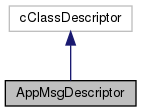
\includegraphics[width=178pt]{class_app_msg_descriptor__inherit__graph}
\end{center}
\end{figure}


Collaboration diagram for App\+Msg\+Descriptor\+:
\nopagebreak
\begin{figure}[H]
\begin{center}
\leavevmode
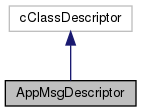
\includegraphics[width=178pt]{class_app_msg_descriptor__coll__graph}
\end{center}
\end{figure}
\subsection*{Public Member Functions}
\begin{DoxyCompactItemize}
\item 
\hyperlink{class_app_msg_descriptor_a6db2ddcf43396f5c9f97311e757e3b51}{App\+Msg\+Descriptor} ()
\item 
virtual \hyperlink{class_app_msg_descriptor_ab164a07b536b9fba949565b8717dc502}{$\sim$\+App\+Msg\+Descriptor} ()
\item 
virtual bool \hyperlink{class_app_msg_descriptor_a46278424168df1b1c695931d232903aa}{does\+Support} (omnetpp\+::c\+Object $\ast$obj) const override
\item 
virtual const char $\ast$$\ast$ \hyperlink{class_app_msg_descriptor_a463f64b1782fbb94c24696f35b3e3060}{get\+Property\+Names} () const override
\item 
virtual const char $\ast$ \hyperlink{class_app_msg_descriptor_a3aeec901180fe34d706eb995bba59e7d}{get\+Property} (const char $\ast$propertyname) const override
\item 
virtual int \hyperlink{class_app_msg_descriptor_a3f448baccbb92d3da8d5026c660a8457}{get\+Field\+Count} () const override
\item 
virtual const char $\ast$ \hyperlink{class_app_msg_descriptor_a65c09ea4375fe8dd56084e1801adbbcd}{get\+Field\+Name} (int field) const override
\item 
virtual int \hyperlink{class_app_msg_descriptor_aeb69344c912887ff0e64d4e4d5d587ba}{find\+Field} (const char $\ast$field\+Name) const override
\item 
virtual unsigned int \hyperlink{class_app_msg_descriptor_a9b354c043d42e40ffe92ccf17a3b49fa}{get\+Field\+Type\+Flags} (int field) const override
\item 
virtual const char $\ast$ \hyperlink{class_app_msg_descriptor_a332a8a40b5013ad50415638e7f0b4ddf}{get\+Field\+Type\+String} (int field) const override
\item 
virtual const char $\ast$$\ast$ \hyperlink{class_app_msg_descriptor_a9cf3ac7e1dc6b2d7262c89736aa77944}{get\+Field\+Property\+Names} (int field) const override
\item 
virtual const char $\ast$ \hyperlink{class_app_msg_descriptor_ae7df10b5c7668b06b562cab7fc5c6e27}{get\+Field\+Property} (int field, const char $\ast$propertyname) const override
\item 
virtual int \hyperlink{class_app_msg_descriptor_a5461c8b2212d7f2060de56ba67c3138e}{get\+Field\+Array\+Size} (void $\ast$object, int field) const override
\item 
virtual const char $\ast$ \hyperlink{class_app_msg_descriptor_a34ca59ce0eb79e96189a0c6f31fa8ce0}{get\+Field\+Dynamic\+Type\+String} (void $\ast$object, int field, int i) const override
\item 
virtual std\+::string \hyperlink{class_app_msg_descriptor_aa43546ba09c6953ecd4fc9e66d16bd76}{get\+Field\+Value\+As\+String} (void $\ast$object, int field, int i) const override
\item 
virtual bool \hyperlink{class_app_msg_descriptor_a0e77c504e3174dfd8c666d286c68b37b}{set\+Field\+Value\+As\+String} (void $\ast$object, int field, int i, const char $\ast$value) const override
\item 
virtual const char $\ast$ \hyperlink{class_app_msg_descriptor_a3879e3c38670b7a85ef43ba4a1ae7408}{get\+Field\+Struct\+Name} (int field) const override
\item 
virtual void $\ast$ \hyperlink{class_app_msg_descriptor_a5eeec27327bfa4d54924a9913006b689}{get\+Field\+Struct\+Value\+Pointer} (void $\ast$object, int field, int i) const override
\end{DoxyCompactItemize}
\subsection*{Private Attributes}
\begin{DoxyCompactItemize}
\item 
const char $\ast$$\ast$ \hyperlink{class_app_msg_descriptor_a4fb3b9dd77f943bb3aa1587c8d28c1c8}{propertynames}
\end{DoxyCompactItemize}


\subsection{Constructor \& Destructor Documentation}
\mbox{\Hypertarget{class_app_msg_descriptor_a6db2ddcf43396f5c9f97311e757e3b51}\label{class_app_msg_descriptor_a6db2ddcf43396f5c9f97311e757e3b51}} 
\index{App\+Msg\+Descriptor@{App\+Msg\+Descriptor}!App\+Msg\+Descriptor@{App\+Msg\+Descriptor}}
\index{App\+Msg\+Descriptor@{App\+Msg\+Descriptor}!App\+Msg\+Descriptor@{App\+Msg\+Descriptor}}
\subsubsection{\texorpdfstring{App\+Msg\+Descriptor()}{AppMsgDescriptor()}}
{\footnotesize\ttfamily App\+Msg\+Descriptor\+::\+App\+Msg\+Descriptor (\begin{DoxyParamCaption}{ }\end{DoxyParamCaption})}

\mbox{\Hypertarget{class_app_msg_descriptor_ab164a07b536b9fba949565b8717dc502}\label{class_app_msg_descriptor_ab164a07b536b9fba949565b8717dc502}} 
\index{App\+Msg\+Descriptor@{App\+Msg\+Descriptor}!````~App\+Msg\+Descriptor@{$\sim$\+App\+Msg\+Descriptor}}
\index{````~App\+Msg\+Descriptor@{$\sim$\+App\+Msg\+Descriptor}!App\+Msg\+Descriptor@{App\+Msg\+Descriptor}}
\subsubsection{\texorpdfstring{$\sim$\+App\+Msg\+Descriptor()}{~AppMsgDescriptor()}}
{\footnotesize\ttfamily App\+Msg\+Descriptor\+::$\sim$\+App\+Msg\+Descriptor (\begin{DoxyParamCaption}{ }\end{DoxyParamCaption})\hspace{0.3cm}{\ttfamily [virtual]}}



\subsection{Member Function Documentation}
\mbox{\Hypertarget{class_app_msg_descriptor_a46278424168df1b1c695931d232903aa}\label{class_app_msg_descriptor_a46278424168df1b1c695931d232903aa}} 
\index{App\+Msg\+Descriptor@{App\+Msg\+Descriptor}!does\+Support@{does\+Support}}
\index{does\+Support@{does\+Support}!App\+Msg\+Descriptor@{App\+Msg\+Descriptor}}
\subsubsection{\texorpdfstring{does\+Support()}{doesSupport()}}
{\footnotesize\ttfamily bool App\+Msg\+Descriptor\+::does\+Support (\begin{DoxyParamCaption}\item[{omnetpp\+::c\+Object $\ast$}]{obj }\end{DoxyParamCaption}) const\hspace{0.3cm}{\ttfamily [override]}, {\ttfamily [virtual]}}

\mbox{\Hypertarget{class_app_msg_descriptor_aeb69344c912887ff0e64d4e4d5d587ba}\label{class_app_msg_descriptor_aeb69344c912887ff0e64d4e4d5d587ba}} 
\index{App\+Msg\+Descriptor@{App\+Msg\+Descriptor}!find\+Field@{find\+Field}}
\index{find\+Field@{find\+Field}!App\+Msg\+Descriptor@{App\+Msg\+Descriptor}}
\subsubsection{\texorpdfstring{find\+Field()}{findField()}}
{\footnotesize\ttfamily int App\+Msg\+Descriptor\+::find\+Field (\begin{DoxyParamCaption}\item[{const char $\ast$}]{field\+Name }\end{DoxyParamCaption}) const\hspace{0.3cm}{\ttfamily [override]}, {\ttfamily [virtual]}}

\mbox{\Hypertarget{class_app_msg_descriptor_a5461c8b2212d7f2060de56ba67c3138e}\label{class_app_msg_descriptor_a5461c8b2212d7f2060de56ba67c3138e}} 
\index{App\+Msg\+Descriptor@{App\+Msg\+Descriptor}!get\+Field\+Array\+Size@{get\+Field\+Array\+Size}}
\index{get\+Field\+Array\+Size@{get\+Field\+Array\+Size}!App\+Msg\+Descriptor@{App\+Msg\+Descriptor}}
\subsubsection{\texorpdfstring{get\+Field\+Array\+Size()}{getFieldArraySize()}}
{\footnotesize\ttfamily int App\+Msg\+Descriptor\+::get\+Field\+Array\+Size (\begin{DoxyParamCaption}\item[{void $\ast$}]{object,  }\item[{int}]{field }\end{DoxyParamCaption}) const\hspace{0.3cm}{\ttfamily [override]}, {\ttfamily [virtual]}}

\mbox{\Hypertarget{class_app_msg_descriptor_a3f448baccbb92d3da8d5026c660a8457}\label{class_app_msg_descriptor_a3f448baccbb92d3da8d5026c660a8457}} 
\index{App\+Msg\+Descriptor@{App\+Msg\+Descriptor}!get\+Field\+Count@{get\+Field\+Count}}
\index{get\+Field\+Count@{get\+Field\+Count}!App\+Msg\+Descriptor@{App\+Msg\+Descriptor}}
\subsubsection{\texorpdfstring{get\+Field\+Count()}{getFieldCount()}}
{\footnotesize\ttfamily int App\+Msg\+Descriptor\+::get\+Field\+Count (\begin{DoxyParamCaption}{ }\end{DoxyParamCaption}) const\hspace{0.3cm}{\ttfamily [override]}, {\ttfamily [virtual]}}

\mbox{\Hypertarget{class_app_msg_descriptor_a34ca59ce0eb79e96189a0c6f31fa8ce0}\label{class_app_msg_descriptor_a34ca59ce0eb79e96189a0c6f31fa8ce0}} 
\index{App\+Msg\+Descriptor@{App\+Msg\+Descriptor}!get\+Field\+Dynamic\+Type\+String@{get\+Field\+Dynamic\+Type\+String}}
\index{get\+Field\+Dynamic\+Type\+String@{get\+Field\+Dynamic\+Type\+String}!App\+Msg\+Descriptor@{App\+Msg\+Descriptor}}
\subsubsection{\texorpdfstring{get\+Field\+Dynamic\+Type\+String()}{getFieldDynamicTypeString()}}
{\footnotesize\ttfamily const char $\ast$ App\+Msg\+Descriptor\+::get\+Field\+Dynamic\+Type\+String (\begin{DoxyParamCaption}\item[{void $\ast$}]{object,  }\item[{int}]{field,  }\item[{int}]{i }\end{DoxyParamCaption}) const\hspace{0.3cm}{\ttfamily [override]}, {\ttfamily [virtual]}}

\mbox{\Hypertarget{class_app_msg_descriptor_a65c09ea4375fe8dd56084e1801adbbcd}\label{class_app_msg_descriptor_a65c09ea4375fe8dd56084e1801adbbcd}} 
\index{App\+Msg\+Descriptor@{App\+Msg\+Descriptor}!get\+Field\+Name@{get\+Field\+Name}}
\index{get\+Field\+Name@{get\+Field\+Name}!App\+Msg\+Descriptor@{App\+Msg\+Descriptor}}
\subsubsection{\texorpdfstring{get\+Field\+Name()}{getFieldName()}}
{\footnotesize\ttfamily const char $\ast$ App\+Msg\+Descriptor\+::get\+Field\+Name (\begin{DoxyParamCaption}\item[{int}]{field }\end{DoxyParamCaption}) const\hspace{0.3cm}{\ttfamily [override]}, {\ttfamily [virtual]}}

\mbox{\Hypertarget{class_app_msg_descriptor_ae7df10b5c7668b06b562cab7fc5c6e27}\label{class_app_msg_descriptor_ae7df10b5c7668b06b562cab7fc5c6e27}} 
\index{App\+Msg\+Descriptor@{App\+Msg\+Descriptor}!get\+Field\+Property@{get\+Field\+Property}}
\index{get\+Field\+Property@{get\+Field\+Property}!App\+Msg\+Descriptor@{App\+Msg\+Descriptor}}
\subsubsection{\texorpdfstring{get\+Field\+Property()}{getFieldProperty()}}
{\footnotesize\ttfamily const char $\ast$ App\+Msg\+Descriptor\+::get\+Field\+Property (\begin{DoxyParamCaption}\item[{int}]{field,  }\item[{const char $\ast$}]{propertyname }\end{DoxyParamCaption}) const\hspace{0.3cm}{\ttfamily [override]}, {\ttfamily [virtual]}}

\mbox{\Hypertarget{class_app_msg_descriptor_a9cf3ac7e1dc6b2d7262c89736aa77944}\label{class_app_msg_descriptor_a9cf3ac7e1dc6b2d7262c89736aa77944}} 
\index{App\+Msg\+Descriptor@{App\+Msg\+Descriptor}!get\+Field\+Property\+Names@{get\+Field\+Property\+Names}}
\index{get\+Field\+Property\+Names@{get\+Field\+Property\+Names}!App\+Msg\+Descriptor@{App\+Msg\+Descriptor}}
\subsubsection{\texorpdfstring{get\+Field\+Property\+Names()}{getFieldPropertyNames()}}
{\footnotesize\ttfamily const char $\ast$$\ast$ App\+Msg\+Descriptor\+::get\+Field\+Property\+Names (\begin{DoxyParamCaption}\item[{int}]{field }\end{DoxyParamCaption}) const\hspace{0.3cm}{\ttfamily [override]}, {\ttfamily [virtual]}}

\mbox{\Hypertarget{class_app_msg_descriptor_a3879e3c38670b7a85ef43ba4a1ae7408}\label{class_app_msg_descriptor_a3879e3c38670b7a85ef43ba4a1ae7408}} 
\index{App\+Msg\+Descriptor@{App\+Msg\+Descriptor}!get\+Field\+Struct\+Name@{get\+Field\+Struct\+Name}}
\index{get\+Field\+Struct\+Name@{get\+Field\+Struct\+Name}!App\+Msg\+Descriptor@{App\+Msg\+Descriptor}}
\subsubsection{\texorpdfstring{get\+Field\+Struct\+Name()}{getFieldStructName()}}
{\footnotesize\ttfamily const char $\ast$ App\+Msg\+Descriptor\+::get\+Field\+Struct\+Name (\begin{DoxyParamCaption}\item[{int}]{field }\end{DoxyParamCaption}) const\hspace{0.3cm}{\ttfamily [override]}, {\ttfamily [virtual]}}

\mbox{\Hypertarget{class_app_msg_descriptor_a5eeec27327bfa4d54924a9913006b689}\label{class_app_msg_descriptor_a5eeec27327bfa4d54924a9913006b689}} 
\index{App\+Msg\+Descriptor@{App\+Msg\+Descriptor}!get\+Field\+Struct\+Value\+Pointer@{get\+Field\+Struct\+Value\+Pointer}}
\index{get\+Field\+Struct\+Value\+Pointer@{get\+Field\+Struct\+Value\+Pointer}!App\+Msg\+Descriptor@{App\+Msg\+Descriptor}}
\subsubsection{\texorpdfstring{get\+Field\+Struct\+Value\+Pointer()}{getFieldStructValuePointer()}}
{\footnotesize\ttfamily void $\ast$ App\+Msg\+Descriptor\+::get\+Field\+Struct\+Value\+Pointer (\begin{DoxyParamCaption}\item[{void $\ast$}]{object,  }\item[{int}]{field,  }\item[{int}]{i }\end{DoxyParamCaption}) const\hspace{0.3cm}{\ttfamily [override]}, {\ttfamily [virtual]}}

\mbox{\Hypertarget{class_app_msg_descriptor_a9b354c043d42e40ffe92ccf17a3b49fa}\label{class_app_msg_descriptor_a9b354c043d42e40ffe92ccf17a3b49fa}} 
\index{App\+Msg\+Descriptor@{App\+Msg\+Descriptor}!get\+Field\+Type\+Flags@{get\+Field\+Type\+Flags}}
\index{get\+Field\+Type\+Flags@{get\+Field\+Type\+Flags}!App\+Msg\+Descriptor@{App\+Msg\+Descriptor}}
\subsubsection{\texorpdfstring{get\+Field\+Type\+Flags()}{getFieldTypeFlags()}}
{\footnotesize\ttfamily unsigned int App\+Msg\+Descriptor\+::get\+Field\+Type\+Flags (\begin{DoxyParamCaption}\item[{int}]{field }\end{DoxyParamCaption}) const\hspace{0.3cm}{\ttfamily [override]}, {\ttfamily [virtual]}}

\mbox{\Hypertarget{class_app_msg_descriptor_a332a8a40b5013ad50415638e7f0b4ddf}\label{class_app_msg_descriptor_a332a8a40b5013ad50415638e7f0b4ddf}} 
\index{App\+Msg\+Descriptor@{App\+Msg\+Descriptor}!get\+Field\+Type\+String@{get\+Field\+Type\+String}}
\index{get\+Field\+Type\+String@{get\+Field\+Type\+String}!App\+Msg\+Descriptor@{App\+Msg\+Descriptor}}
\subsubsection{\texorpdfstring{get\+Field\+Type\+String()}{getFieldTypeString()}}
{\footnotesize\ttfamily const char $\ast$ App\+Msg\+Descriptor\+::get\+Field\+Type\+String (\begin{DoxyParamCaption}\item[{int}]{field }\end{DoxyParamCaption}) const\hspace{0.3cm}{\ttfamily [override]}, {\ttfamily [virtual]}}

\mbox{\Hypertarget{class_app_msg_descriptor_aa43546ba09c6953ecd4fc9e66d16bd76}\label{class_app_msg_descriptor_aa43546ba09c6953ecd4fc9e66d16bd76}} 
\index{App\+Msg\+Descriptor@{App\+Msg\+Descriptor}!get\+Field\+Value\+As\+String@{get\+Field\+Value\+As\+String}}
\index{get\+Field\+Value\+As\+String@{get\+Field\+Value\+As\+String}!App\+Msg\+Descriptor@{App\+Msg\+Descriptor}}
\subsubsection{\texorpdfstring{get\+Field\+Value\+As\+String()}{getFieldValueAsString()}}
{\footnotesize\ttfamily std\+::string App\+Msg\+Descriptor\+::get\+Field\+Value\+As\+String (\begin{DoxyParamCaption}\item[{void $\ast$}]{object,  }\item[{int}]{field,  }\item[{int}]{i }\end{DoxyParamCaption}) const\hspace{0.3cm}{\ttfamily [override]}, {\ttfamily [virtual]}}

\mbox{\Hypertarget{class_app_msg_descriptor_a3aeec901180fe34d706eb995bba59e7d}\label{class_app_msg_descriptor_a3aeec901180fe34d706eb995bba59e7d}} 
\index{App\+Msg\+Descriptor@{App\+Msg\+Descriptor}!get\+Property@{get\+Property}}
\index{get\+Property@{get\+Property}!App\+Msg\+Descriptor@{App\+Msg\+Descriptor}}
\subsubsection{\texorpdfstring{get\+Property()}{getProperty()}}
{\footnotesize\ttfamily const char $\ast$ App\+Msg\+Descriptor\+::get\+Property (\begin{DoxyParamCaption}\item[{const char $\ast$}]{propertyname }\end{DoxyParamCaption}) const\hspace{0.3cm}{\ttfamily [override]}, {\ttfamily [virtual]}}

\mbox{\Hypertarget{class_app_msg_descriptor_a463f64b1782fbb94c24696f35b3e3060}\label{class_app_msg_descriptor_a463f64b1782fbb94c24696f35b3e3060}} 
\index{App\+Msg\+Descriptor@{App\+Msg\+Descriptor}!get\+Property\+Names@{get\+Property\+Names}}
\index{get\+Property\+Names@{get\+Property\+Names}!App\+Msg\+Descriptor@{App\+Msg\+Descriptor}}
\subsubsection{\texorpdfstring{get\+Property\+Names()}{getPropertyNames()}}
{\footnotesize\ttfamily const char $\ast$$\ast$ App\+Msg\+Descriptor\+::get\+Property\+Names (\begin{DoxyParamCaption}{ }\end{DoxyParamCaption}) const\hspace{0.3cm}{\ttfamily [override]}, {\ttfamily [virtual]}}

\mbox{\Hypertarget{class_app_msg_descriptor_a0e77c504e3174dfd8c666d286c68b37b}\label{class_app_msg_descriptor_a0e77c504e3174dfd8c666d286c68b37b}} 
\index{App\+Msg\+Descriptor@{App\+Msg\+Descriptor}!set\+Field\+Value\+As\+String@{set\+Field\+Value\+As\+String}}
\index{set\+Field\+Value\+As\+String@{set\+Field\+Value\+As\+String}!App\+Msg\+Descriptor@{App\+Msg\+Descriptor}}
\subsubsection{\texorpdfstring{set\+Field\+Value\+As\+String()}{setFieldValueAsString()}}
{\footnotesize\ttfamily bool App\+Msg\+Descriptor\+::set\+Field\+Value\+As\+String (\begin{DoxyParamCaption}\item[{void $\ast$}]{object,  }\item[{int}]{field,  }\item[{int}]{i,  }\item[{const char $\ast$}]{value }\end{DoxyParamCaption}) const\hspace{0.3cm}{\ttfamily [override]}, {\ttfamily [virtual]}}



\subsection{Member Data Documentation}
\mbox{\Hypertarget{class_app_msg_descriptor_a4fb3b9dd77f943bb3aa1587c8d28c1c8}\label{class_app_msg_descriptor_a4fb3b9dd77f943bb3aa1587c8d28c1c8}} 
\index{App\+Msg\+Descriptor@{App\+Msg\+Descriptor}!propertynames@{propertynames}}
\index{propertynames@{propertynames}!App\+Msg\+Descriptor@{App\+Msg\+Descriptor}}
\subsubsection{\texorpdfstring{propertynames}{propertynames}}
{\footnotesize\ttfamily const char$\ast$$\ast$ App\+Msg\+Descriptor\+::propertynames\hspace{0.3cm}{\ttfamily [mutable]}, {\ttfamily [private]}}



The documentation for this class was generated from the following file\+:\begin{DoxyCompactItemize}
\item 
/home/wilhelm/\+Documents/code\+Git\+Hub/\+Error\+Detectors/src/\+Messages/\hyperlink{_app_msg__m_8cc}{App\+Msg\+\_\+m.\+cc}\end{DoxyCompactItemize}

\hypertarget{class_app_msg_false_dep_descriptor}{}\section{App\+Msg\+False\+Dep\+Descriptor Class Reference}
\label{class_app_msg_false_dep_descriptor}\index{App\+Msg\+False\+Dep\+Descriptor@{App\+Msg\+False\+Dep\+Descriptor}}


Inheritance diagram for App\+Msg\+False\+Dep\+Descriptor\+:\nopagebreak
\begin{figure}[H]
\begin{center}
\leavevmode
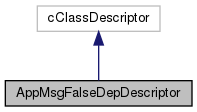
\includegraphics[width=220pt]{class_app_msg_false_dep_descriptor__inherit__graph}
\end{center}
\end{figure}


Collaboration diagram for App\+Msg\+False\+Dep\+Descriptor\+:\nopagebreak
\begin{figure}[H]
\begin{center}
\leavevmode
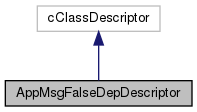
\includegraphics[width=220pt]{class_app_msg_false_dep_descriptor__coll__graph}
\end{center}
\end{figure}
\subsection*{Public Member Functions}
\begin{DoxyCompactItemize}
\item 
\hyperlink{class_app_msg_false_dep_descriptor_a4ca99cc9f908534f473db357ba25ff2d}{App\+Msg\+False\+Dep\+Descriptor} ()
\item 
virtual \hyperlink{class_app_msg_false_dep_descriptor_a8d7c2d85fad2a90a6cd377ae150345a0}{$\sim$\+App\+Msg\+False\+Dep\+Descriptor} ()
\item 
virtual bool \hyperlink{class_app_msg_false_dep_descriptor_ac3fc2e2a9ff6986bec98c724590aa456}{does\+Support} (omnetpp\+::c\+Object $\ast$obj) const override
\item 
virtual const char $\ast$$\ast$ \hyperlink{class_app_msg_false_dep_descriptor_a550ade508a3c3d84d5781aba6bf02ec8}{get\+Property\+Names} () const override
\item 
virtual const char $\ast$ \hyperlink{class_app_msg_false_dep_descriptor_ac5650d0cbf554966c9fa8a1add231af7}{get\+Property} (const char $\ast$propertyname) const override
\item 
virtual int \hyperlink{class_app_msg_false_dep_descriptor_ade54239f119054d3995dc4e7570718a9}{get\+Field\+Count} () const override
\item 
virtual const char $\ast$ \hyperlink{class_app_msg_false_dep_descriptor_ae89f0e9b564147c2faa20b8ffc47a2bb}{get\+Field\+Name} (int field) const override
\item 
virtual int \hyperlink{class_app_msg_false_dep_descriptor_a9c9cfe9dbacb64401882bc7c4d0e7ef1}{find\+Field} (const char $\ast$field\+Name) const override
\item 
virtual unsigned int \hyperlink{class_app_msg_false_dep_descriptor_a09a72b309888cf637248490b2482e435}{get\+Field\+Type\+Flags} (int field) const override
\item 
virtual const char $\ast$ \hyperlink{class_app_msg_false_dep_descriptor_a83e838bc58a595cfbfe43a9a4ccabb2e}{get\+Field\+Type\+String} (int field) const override
\item 
virtual const char $\ast$$\ast$ \hyperlink{class_app_msg_false_dep_descriptor_a73becb0b27a833d32fde15e0b9b87572}{get\+Field\+Property\+Names} (int field) const override
\item 
virtual const char $\ast$ \hyperlink{class_app_msg_false_dep_descriptor_a9737ecde44ab7bd573cdd94edc494b2f}{get\+Field\+Property} (int field, const char $\ast$propertyname) const override
\item 
virtual int \hyperlink{class_app_msg_false_dep_descriptor_a179d2851182b7e2c778befc442640361}{get\+Field\+Array\+Size} (void $\ast$object, int field) const override
\item 
virtual const char $\ast$ \hyperlink{class_app_msg_false_dep_descriptor_a18f649fae5364f7b9f326fd1ae9afb6d}{get\+Field\+Dynamic\+Type\+String} (void $\ast$object, int field, int i) const override
\item 
virtual std\+::string \hyperlink{class_app_msg_false_dep_descriptor_ac9b26b1e9c849df0e0259dfa3a38885c}{get\+Field\+Value\+As\+String} (void $\ast$object, int field, int i) const override
\item 
virtual bool \hyperlink{class_app_msg_false_dep_descriptor_ad7f784c5c9c941292342602674c4b9e4}{set\+Field\+Value\+As\+String} (void $\ast$object, int field, int i, const char $\ast$value) const override
\item 
virtual const char $\ast$ \hyperlink{class_app_msg_false_dep_descriptor_aa44a321c042bf2af6eff2f92ad52f73d}{get\+Field\+Struct\+Name} (int field) const override
\item 
virtual void $\ast$ \hyperlink{class_app_msg_false_dep_descriptor_a2975e01f5455360c1954f722dfce0924}{get\+Field\+Struct\+Value\+Pointer} (void $\ast$object, int field, int i) const override
\end{DoxyCompactItemize}
\subsection*{Private Attributes}
\begin{DoxyCompactItemize}
\item 
const char $\ast$$\ast$ \hyperlink{class_app_msg_false_dep_descriptor_a9ae1f3f2f3bd0f3647643894402add0b}{propertynames}
\end{DoxyCompactItemize}


\subsection{Constructor \& Destructor Documentation}
\mbox{\Hypertarget{class_app_msg_false_dep_descriptor_a4ca99cc9f908534f473db357ba25ff2d}\label{class_app_msg_false_dep_descriptor_a4ca99cc9f908534f473db357ba25ff2d}} 
\index{App\+Msg\+False\+Dep\+Descriptor@{App\+Msg\+False\+Dep\+Descriptor}!App\+Msg\+False\+Dep\+Descriptor@{App\+Msg\+False\+Dep\+Descriptor}}
\index{App\+Msg\+False\+Dep\+Descriptor@{App\+Msg\+False\+Dep\+Descriptor}!App\+Msg\+False\+Dep\+Descriptor@{App\+Msg\+False\+Dep\+Descriptor}}
\subsubsection{\texorpdfstring{App\+Msg\+False\+Dep\+Descriptor()}{AppMsgFalseDepDescriptor()}}
{\footnotesize\ttfamily App\+Msg\+False\+Dep\+Descriptor\+::\+App\+Msg\+False\+Dep\+Descriptor (\begin{DoxyParamCaption}{ }\end{DoxyParamCaption})}

\mbox{\Hypertarget{class_app_msg_false_dep_descriptor_a8d7c2d85fad2a90a6cd377ae150345a0}\label{class_app_msg_false_dep_descriptor_a8d7c2d85fad2a90a6cd377ae150345a0}} 
\index{App\+Msg\+False\+Dep\+Descriptor@{App\+Msg\+False\+Dep\+Descriptor}!````~App\+Msg\+False\+Dep\+Descriptor@{$\sim$\+App\+Msg\+False\+Dep\+Descriptor}}
\index{````~App\+Msg\+False\+Dep\+Descriptor@{$\sim$\+App\+Msg\+False\+Dep\+Descriptor}!App\+Msg\+False\+Dep\+Descriptor@{App\+Msg\+False\+Dep\+Descriptor}}
\subsubsection{\texorpdfstring{$\sim$\+App\+Msg\+False\+Dep\+Descriptor()}{~AppMsgFalseDepDescriptor()}}
{\footnotesize\ttfamily App\+Msg\+False\+Dep\+Descriptor\+::$\sim$\+App\+Msg\+False\+Dep\+Descriptor (\begin{DoxyParamCaption}{ }\end{DoxyParamCaption})\hspace{0.3cm}{\ttfamily [virtual]}}



\subsection{Member Function Documentation}
\mbox{\Hypertarget{class_app_msg_false_dep_descriptor_ac3fc2e2a9ff6986bec98c724590aa456}\label{class_app_msg_false_dep_descriptor_ac3fc2e2a9ff6986bec98c724590aa456}} 
\index{App\+Msg\+False\+Dep\+Descriptor@{App\+Msg\+False\+Dep\+Descriptor}!does\+Support@{does\+Support}}
\index{does\+Support@{does\+Support}!App\+Msg\+False\+Dep\+Descriptor@{App\+Msg\+False\+Dep\+Descriptor}}
\subsubsection{\texorpdfstring{does\+Support()}{doesSupport()}}
{\footnotesize\ttfamily bool App\+Msg\+False\+Dep\+Descriptor\+::does\+Support (\begin{DoxyParamCaption}\item[{omnetpp\+::c\+Object $\ast$}]{obj }\end{DoxyParamCaption}) const\hspace{0.3cm}{\ttfamily [override]}, {\ttfamily [virtual]}}

\mbox{\Hypertarget{class_app_msg_false_dep_descriptor_a9c9cfe9dbacb64401882bc7c4d0e7ef1}\label{class_app_msg_false_dep_descriptor_a9c9cfe9dbacb64401882bc7c4d0e7ef1}} 
\index{App\+Msg\+False\+Dep\+Descriptor@{App\+Msg\+False\+Dep\+Descriptor}!find\+Field@{find\+Field}}
\index{find\+Field@{find\+Field}!App\+Msg\+False\+Dep\+Descriptor@{App\+Msg\+False\+Dep\+Descriptor}}
\subsubsection{\texorpdfstring{find\+Field()}{findField()}}
{\footnotesize\ttfamily int App\+Msg\+False\+Dep\+Descriptor\+::find\+Field (\begin{DoxyParamCaption}\item[{const char $\ast$}]{field\+Name }\end{DoxyParamCaption}) const\hspace{0.3cm}{\ttfamily [override]}, {\ttfamily [virtual]}}

\mbox{\Hypertarget{class_app_msg_false_dep_descriptor_a179d2851182b7e2c778befc442640361}\label{class_app_msg_false_dep_descriptor_a179d2851182b7e2c778befc442640361}} 
\index{App\+Msg\+False\+Dep\+Descriptor@{App\+Msg\+False\+Dep\+Descriptor}!get\+Field\+Array\+Size@{get\+Field\+Array\+Size}}
\index{get\+Field\+Array\+Size@{get\+Field\+Array\+Size}!App\+Msg\+False\+Dep\+Descriptor@{App\+Msg\+False\+Dep\+Descriptor}}
\subsubsection{\texorpdfstring{get\+Field\+Array\+Size()}{getFieldArraySize()}}
{\footnotesize\ttfamily int App\+Msg\+False\+Dep\+Descriptor\+::get\+Field\+Array\+Size (\begin{DoxyParamCaption}\item[{void $\ast$}]{object,  }\item[{int}]{field }\end{DoxyParamCaption}) const\hspace{0.3cm}{\ttfamily [override]}, {\ttfamily [virtual]}}

\mbox{\Hypertarget{class_app_msg_false_dep_descriptor_ade54239f119054d3995dc4e7570718a9}\label{class_app_msg_false_dep_descriptor_ade54239f119054d3995dc4e7570718a9}} 
\index{App\+Msg\+False\+Dep\+Descriptor@{App\+Msg\+False\+Dep\+Descriptor}!get\+Field\+Count@{get\+Field\+Count}}
\index{get\+Field\+Count@{get\+Field\+Count}!App\+Msg\+False\+Dep\+Descriptor@{App\+Msg\+False\+Dep\+Descriptor}}
\subsubsection{\texorpdfstring{get\+Field\+Count()}{getFieldCount()}}
{\footnotesize\ttfamily int App\+Msg\+False\+Dep\+Descriptor\+::get\+Field\+Count (\begin{DoxyParamCaption}{ }\end{DoxyParamCaption}) const\hspace{0.3cm}{\ttfamily [override]}, {\ttfamily [virtual]}}

\mbox{\Hypertarget{class_app_msg_false_dep_descriptor_a18f649fae5364f7b9f326fd1ae9afb6d}\label{class_app_msg_false_dep_descriptor_a18f649fae5364f7b9f326fd1ae9afb6d}} 
\index{App\+Msg\+False\+Dep\+Descriptor@{App\+Msg\+False\+Dep\+Descriptor}!get\+Field\+Dynamic\+Type\+String@{get\+Field\+Dynamic\+Type\+String}}
\index{get\+Field\+Dynamic\+Type\+String@{get\+Field\+Dynamic\+Type\+String}!App\+Msg\+False\+Dep\+Descriptor@{App\+Msg\+False\+Dep\+Descriptor}}
\subsubsection{\texorpdfstring{get\+Field\+Dynamic\+Type\+String()}{getFieldDynamicTypeString()}}
{\footnotesize\ttfamily const char $\ast$ App\+Msg\+False\+Dep\+Descriptor\+::get\+Field\+Dynamic\+Type\+String (\begin{DoxyParamCaption}\item[{void $\ast$}]{object,  }\item[{int}]{field,  }\item[{int}]{i }\end{DoxyParamCaption}) const\hspace{0.3cm}{\ttfamily [override]}, {\ttfamily [virtual]}}

\mbox{\Hypertarget{class_app_msg_false_dep_descriptor_ae89f0e9b564147c2faa20b8ffc47a2bb}\label{class_app_msg_false_dep_descriptor_ae89f0e9b564147c2faa20b8ffc47a2bb}} 
\index{App\+Msg\+False\+Dep\+Descriptor@{App\+Msg\+False\+Dep\+Descriptor}!get\+Field\+Name@{get\+Field\+Name}}
\index{get\+Field\+Name@{get\+Field\+Name}!App\+Msg\+False\+Dep\+Descriptor@{App\+Msg\+False\+Dep\+Descriptor}}
\subsubsection{\texorpdfstring{get\+Field\+Name()}{getFieldName()}}
{\footnotesize\ttfamily const char $\ast$ App\+Msg\+False\+Dep\+Descriptor\+::get\+Field\+Name (\begin{DoxyParamCaption}\item[{int}]{field }\end{DoxyParamCaption}) const\hspace{0.3cm}{\ttfamily [override]}, {\ttfamily [virtual]}}

\mbox{\Hypertarget{class_app_msg_false_dep_descriptor_a9737ecde44ab7bd573cdd94edc494b2f}\label{class_app_msg_false_dep_descriptor_a9737ecde44ab7bd573cdd94edc494b2f}} 
\index{App\+Msg\+False\+Dep\+Descriptor@{App\+Msg\+False\+Dep\+Descriptor}!get\+Field\+Property@{get\+Field\+Property}}
\index{get\+Field\+Property@{get\+Field\+Property}!App\+Msg\+False\+Dep\+Descriptor@{App\+Msg\+False\+Dep\+Descriptor}}
\subsubsection{\texorpdfstring{get\+Field\+Property()}{getFieldProperty()}}
{\footnotesize\ttfamily const char $\ast$ App\+Msg\+False\+Dep\+Descriptor\+::get\+Field\+Property (\begin{DoxyParamCaption}\item[{int}]{field,  }\item[{const char $\ast$}]{propertyname }\end{DoxyParamCaption}) const\hspace{0.3cm}{\ttfamily [override]}, {\ttfamily [virtual]}}

\mbox{\Hypertarget{class_app_msg_false_dep_descriptor_a73becb0b27a833d32fde15e0b9b87572}\label{class_app_msg_false_dep_descriptor_a73becb0b27a833d32fde15e0b9b87572}} 
\index{App\+Msg\+False\+Dep\+Descriptor@{App\+Msg\+False\+Dep\+Descriptor}!get\+Field\+Property\+Names@{get\+Field\+Property\+Names}}
\index{get\+Field\+Property\+Names@{get\+Field\+Property\+Names}!App\+Msg\+False\+Dep\+Descriptor@{App\+Msg\+False\+Dep\+Descriptor}}
\subsubsection{\texorpdfstring{get\+Field\+Property\+Names()}{getFieldPropertyNames()}}
{\footnotesize\ttfamily const char $\ast$$\ast$ App\+Msg\+False\+Dep\+Descriptor\+::get\+Field\+Property\+Names (\begin{DoxyParamCaption}\item[{int}]{field }\end{DoxyParamCaption}) const\hspace{0.3cm}{\ttfamily [override]}, {\ttfamily [virtual]}}

\mbox{\Hypertarget{class_app_msg_false_dep_descriptor_aa44a321c042bf2af6eff2f92ad52f73d}\label{class_app_msg_false_dep_descriptor_aa44a321c042bf2af6eff2f92ad52f73d}} 
\index{App\+Msg\+False\+Dep\+Descriptor@{App\+Msg\+False\+Dep\+Descriptor}!get\+Field\+Struct\+Name@{get\+Field\+Struct\+Name}}
\index{get\+Field\+Struct\+Name@{get\+Field\+Struct\+Name}!App\+Msg\+False\+Dep\+Descriptor@{App\+Msg\+False\+Dep\+Descriptor}}
\subsubsection{\texorpdfstring{get\+Field\+Struct\+Name()}{getFieldStructName()}}
{\footnotesize\ttfamily const char $\ast$ App\+Msg\+False\+Dep\+Descriptor\+::get\+Field\+Struct\+Name (\begin{DoxyParamCaption}\item[{int}]{field }\end{DoxyParamCaption}) const\hspace{0.3cm}{\ttfamily [override]}, {\ttfamily [virtual]}}

\mbox{\Hypertarget{class_app_msg_false_dep_descriptor_a2975e01f5455360c1954f722dfce0924}\label{class_app_msg_false_dep_descriptor_a2975e01f5455360c1954f722dfce0924}} 
\index{App\+Msg\+False\+Dep\+Descriptor@{App\+Msg\+False\+Dep\+Descriptor}!get\+Field\+Struct\+Value\+Pointer@{get\+Field\+Struct\+Value\+Pointer}}
\index{get\+Field\+Struct\+Value\+Pointer@{get\+Field\+Struct\+Value\+Pointer}!App\+Msg\+False\+Dep\+Descriptor@{App\+Msg\+False\+Dep\+Descriptor}}
\subsubsection{\texorpdfstring{get\+Field\+Struct\+Value\+Pointer()}{getFieldStructValuePointer()}}
{\footnotesize\ttfamily void $\ast$ App\+Msg\+False\+Dep\+Descriptor\+::get\+Field\+Struct\+Value\+Pointer (\begin{DoxyParamCaption}\item[{void $\ast$}]{object,  }\item[{int}]{field,  }\item[{int}]{i }\end{DoxyParamCaption}) const\hspace{0.3cm}{\ttfamily [override]}, {\ttfamily [virtual]}}

\mbox{\Hypertarget{class_app_msg_false_dep_descriptor_a09a72b309888cf637248490b2482e435}\label{class_app_msg_false_dep_descriptor_a09a72b309888cf637248490b2482e435}} 
\index{App\+Msg\+False\+Dep\+Descriptor@{App\+Msg\+False\+Dep\+Descriptor}!get\+Field\+Type\+Flags@{get\+Field\+Type\+Flags}}
\index{get\+Field\+Type\+Flags@{get\+Field\+Type\+Flags}!App\+Msg\+False\+Dep\+Descriptor@{App\+Msg\+False\+Dep\+Descriptor}}
\subsubsection{\texorpdfstring{get\+Field\+Type\+Flags()}{getFieldTypeFlags()}}
{\footnotesize\ttfamily unsigned int App\+Msg\+False\+Dep\+Descriptor\+::get\+Field\+Type\+Flags (\begin{DoxyParamCaption}\item[{int}]{field }\end{DoxyParamCaption}) const\hspace{0.3cm}{\ttfamily [override]}, {\ttfamily [virtual]}}

\mbox{\Hypertarget{class_app_msg_false_dep_descriptor_a83e838bc58a595cfbfe43a9a4ccabb2e}\label{class_app_msg_false_dep_descriptor_a83e838bc58a595cfbfe43a9a4ccabb2e}} 
\index{App\+Msg\+False\+Dep\+Descriptor@{App\+Msg\+False\+Dep\+Descriptor}!get\+Field\+Type\+String@{get\+Field\+Type\+String}}
\index{get\+Field\+Type\+String@{get\+Field\+Type\+String}!App\+Msg\+False\+Dep\+Descriptor@{App\+Msg\+False\+Dep\+Descriptor}}
\subsubsection{\texorpdfstring{get\+Field\+Type\+String()}{getFieldTypeString()}}
{\footnotesize\ttfamily const char $\ast$ App\+Msg\+False\+Dep\+Descriptor\+::get\+Field\+Type\+String (\begin{DoxyParamCaption}\item[{int}]{field }\end{DoxyParamCaption}) const\hspace{0.3cm}{\ttfamily [override]}, {\ttfamily [virtual]}}

\mbox{\Hypertarget{class_app_msg_false_dep_descriptor_ac9b26b1e9c849df0e0259dfa3a38885c}\label{class_app_msg_false_dep_descriptor_ac9b26b1e9c849df0e0259dfa3a38885c}} 
\index{App\+Msg\+False\+Dep\+Descriptor@{App\+Msg\+False\+Dep\+Descriptor}!get\+Field\+Value\+As\+String@{get\+Field\+Value\+As\+String}}
\index{get\+Field\+Value\+As\+String@{get\+Field\+Value\+As\+String}!App\+Msg\+False\+Dep\+Descriptor@{App\+Msg\+False\+Dep\+Descriptor}}
\subsubsection{\texorpdfstring{get\+Field\+Value\+As\+String()}{getFieldValueAsString()}}
{\footnotesize\ttfamily std\+::string App\+Msg\+False\+Dep\+Descriptor\+::get\+Field\+Value\+As\+String (\begin{DoxyParamCaption}\item[{void $\ast$}]{object,  }\item[{int}]{field,  }\item[{int}]{i }\end{DoxyParamCaption}) const\hspace{0.3cm}{\ttfamily [override]}, {\ttfamily [virtual]}}

\mbox{\Hypertarget{class_app_msg_false_dep_descriptor_ac5650d0cbf554966c9fa8a1add231af7}\label{class_app_msg_false_dep_descriptor_ac5650d0cbf554966c9fa8a1add231af7}} 
\index{App\+Msg\+False\+Dep\+Descriptor@{App\+Msg\+False\+Dep\+Descriptor}!get\+Property@{get\+Property}}
\index{get\+Property@{get\+Property}!App\+Msg\+False\+Dep\+Descriptor@{App\+Msg\+False\+Dep\+Descriptor}}
\subsubsection{\texorpdfstring{get\+Property()}{getProperty()}}
{\footnotesize\ttfamily const char $\ast$ App\+Msg\+False\+Dep\+Descriptor\+::get\+Property (\begin{DoxyParamCaption}\item[{const char $\ast$}]{propertyname }\end{DoxyParamCaption}) const\hspace{0.3cm}{\ttfamily [override]}, {\ttfamily [virtual]}}

\mbox{\Hypertarget{class_app_msg_false_dep_descriptor_a550ade508a3c3d84d5781aba6bf02ec8}\label{class_app_msg_false_dep_descriptor_a550ade508a3c3d84d5781aba6bf02ec8}} 
\index{App\+Msg\+False\+Dep\+Descriptor@{App\+Msg\+False\+Dep\+Descriptor}!get\+Property\+Names@{get\+Property\+Names}}
\index{get\+Property\+Names@{get\+Property\+Names}!App\+Msg\+False\+Dep\+Descriptor@{App\+Msg\+False\+Dep\+Descriptor}}
\subsubsection{\texorpdfstring{get\+Property\+Names()}{getPropertyNames()}}
{\footnotesize\ttfamily const char $\ast$$\ast$ App\+Msg\+False\+Dep\+Descriptor\+::get\+Property\+Names (\begin{DoxyParamCaption}{ }\end{DoxyParamCaption}) const\hspace{0.3cm}{\ttfamily [override]}, {\ttfamily [virtual]}}

\mbox{\Hypertarget{class_app_msg_false_dep_descriptor_ad7f784c5c9c941292342602674c4b9e4}\label{class_app_msg_false_dep_descriptor_ad7f784c5c9c941292342602674c4b9e4}} 
\index{App\+Msg\+False\+Dep\+Descriptor@{App\+Msg\+False\+Dep\+Descriptor}!set\+Field\+Value\+As\+String@{set\+Field\+Value\+As\+String}}
\index{set\+Field\+Value\+As\+String@{set\+Field\+Value\+As\+String}!App\+Msg\+False\+Dep\+Descriptor@{App\+Msg\+False\+Dep\+Descriptor}}
\subsubsection{\texorpdfstring{set\+Field\+Value\+As\+String()}{setFieldValueAsString()}}
{\footnotesize\ttfamily bool App\+Msg\+False\+Dep\+Descriptor\+::set\+Field\+Value\+As\+String (\begin{DoxyParamCaption}\item[{void $\ast$}]{object,  }\item[{int}]{field,  }\item[{int}]{i,  }\item[{const char $\ast$}]{value }\end{DoxyParamCaption}) const\hspace{0.3cm}{\ttfamily [override]}, {\ttfamily [virtual]}}



\subsection{Member Data Documentation}
\mbox{\Hypertarget{class_app_msg_false_dep_descriptor_a9ae1f3f2f3bd0f3647643894402add0b}\label{class_app_msg_false_dep_descriptor_a9ae1f3f2f3bd0f3647643894402add0b}} 
\index{App\+Msg\+False\+Dep\+Descriptor@{App\+Msg\+False\+Dep\+Descriptor}!propertynames@{propertynames}}
\index{propertynames@{propertynames}!App\+Msg\+False\+Dep\+Descriptor@{App\+Msg\+False\+Dep\+Descriptor}}
\subsubsection{\texorpdfstring{propertynames}{propertynames}}
{\footnotesize\ttfamily const char$\ast$$\ast$ App\+Msg\+False\+Dep\+Descriptor\+::propertynames\hspace{0.3cm}{\ttfamily [mutable]}, {\ttfamily [private]}}



The documentation for this class was generated from the following file\+:\begin{DoxyCompactItemize}
\item 
src/\+Messages/\hyperlink{_app_msg__m_8cc}{App\+Msg\+\_\+m.\+cc}\end{DoxyCompactItemize}

\hypertarget{class_app_msg_p_c_descriptor}{}\section{App\+Msg\+P\+C\+Descriptor Class Reference}
\label{class_app_msg_p_c_descriptor}\index{App\+Msg\+P\+C\+Descriptor@{App\+Msg\+P\+C\+Descriptor}}


Inheritance diagram for App\+Msg\+P\+C\+Descriptor\+:
\nopagebreak
\begin{figure}[H]
\begin{center}
\leavevmode
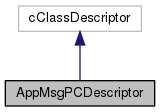
\includegraphics[width=192pt]{class_app_msg_p_c_descriptor__inherit__graph}
\end{center}
\end{figure}


Collaboration diagram for App\+Msg\+P\+C\+Descriptor\+:
\nopagebreak
\begin{figure}[H]
\begin{center}
\leavevmode
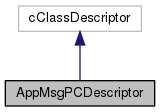
\includegraphics[width=192pt]{class_app_msg_p_c_descriptor__coll__graph}
\end{center}
\end{figure}
\subsection*{Public Member Functions}
\begin{DoxyCompactItemize}
\item 
\hyperlink{class_app_msg_p_c_descriptor_a3a331f63d98d56b7433d83ad6afd2fa1}{App\+Msg\+P\+C\+Descriptor} ()
\item 
virtual \hyperlink{class_app_msg_p_c_descriptor_a7928920541dd96935380cd468ee51d5a}{$\sim$\+App\+Msg\+P\+C\+Descriptor} ()
\item 
virtual bool \hyperlink{class_app_msg_p_c_descriptor_a198ed191c1c36b7b177779ab6c36be01}{does\+Support} (omnetpp\+::c\+Object $\ast$obj) const override
\item 
virtual const char $\ast$$\ast$ \hyperlink{class_app_msg_p_c_descriptor_a4e178c3b5f9cca9e86b4e858d3964de7}{get\+Property\+Names} () const override
\item 
virtual const char $\ast$ \hyperlink{class_app_msg_p_c_descriptor_aa3e2e1730d4446da261f56a6c62b8703}{get\+Property} (const char $\ast$propertyname) const override
\item 
virtual int \hyperlink{class_app_msg_p_c_descriptor_a2936e9fbdd28e56c2197380ada446d5e}{get\+Field\+Count} () const override
\item 
virtual const char $\ast$ \hyperlink{class_app_msg_p_c_descriptor_aa147246f0555048fc684ce8bdbf4964f}{get\+Field\+Name} (int field) const override
\item 
virtual int \hyperlink{class_app_msg_p_c_descriptor_a23a276307871f95930bf7f03df3fb178}{find\+Field} (const char $\ast$field\+Name) const override
\item 
virtual unsigned int \hyperlink{class_app_msg_p_c_descriptor_ab112abe6a70f75081cd176586e9ac6d4}{get\+Field\+Type\+Flags} (int field) const override
\item 
virtual const char $\ast$ \hyperlink{class_app_msg_p_c_descriptor_aa5a22389b1a0d2b8e97c936f69a2ed39}{get\+Field\+Type\+String} (int field) const override
\item 
virtual const char $\ast$$\ast$ \hyperlink{class_app_msg_p_c_descriptor_a36f69eac7b710983aa66c647ca0a15c8}{get\+Field\+Property\+Names} (int field) const override
\item 
virtual const char $\ast$ \hyperlink{class_app_msg_p_c_descriptor_a1c141ad9ba88b4113c35424827a46ee9}{get\+Field\+Property} (int field, const char $\ast$propertyname) const override
\item 
virtual int \hyperlink{class_app_msg_p_c_descriptor_abd0b0ccd2b54ad45825704c566922f67}{get\+Field\+Array\+Size} (void $\ast$object, int field) const override
\item 
virtual const char $\ast$ \hyperlink{class_app_msg_p_c_descriptor_a17016d018e18d544b226ecd3119de5b2}{get\+Field\+Dynamic\+Type\+String} (void $\ast$object, int field, int i) const override
\item 
virtual std\+::string \hyperlink{class_app_msg_p_c_descriptor_ac5f4467bbe2dae35c300f7288bfc4003}{get\+Field\+Value\+As\+String} (void $\ast$object, int field, int i) const override
\item 
virtual bool \hyperlink{class_app_msg_p_c_descriptor_a8eecfb063c75f3c72ceb3646680b9261}{set\+Field\+Value\+As\+String} (void $\ast$object, int field, int i, const char $\ast$value) const override
\item 
virtual const char $\ast$ \hyperlink{class_app_msg_p_c_descriptor_a10b8057293b17adac40060a533966cf8}{get\+Field\+Struct\+Name} (int field) const override
\item 
virtual void $\ast$ \hyperlink{class_app_msg_p_c_descriptor_aaeff42267f2ab084ef76f8bf9eb0eedd}{get\+Field\+Struct\+Value\+Pointer} (void $\ast$object, int field, int i) const override
\end{DoxyCompactItemize}
\subsection*{Private Attributes}
\begin{DoxyCompactItemize}
\item 
const char $\ast$$\ast$ \hyperlink{class_app_msg_p_c_descriptor_aaeca386eddf80dd71ff4cdd3bb1353a7}{propertynames}
\end{DoxyCompactItemize}


\subsection{Constructor \& Destructor Documentation}
\mbox{\Hypertarget{class_app_msg_p_c_descriptor_a3a331f63d98d56b7433d83ad6afd2fa1}\label{class_app_msg_p_c_descriptor_a3a331f63d98d56b7433d83ad6afd2fa1}} 
\index{App\+Msg\+P\+C\+Descriptor@{App\+Msg\+P\+C\+Descriptor}!App\+Msg\+P\+C\+Descriptor@{App\+Msg\+P\+C\+Descriptor}}
\index{App\+Msg\+P\+C\+Descriptor@{App\+Msg\+P\+C\+Descriptor}!App\+Msg\+P\+C\+Descriptor@{App\+Msg\+P\+C\+Descriptor}}
\subsubsection{\texorpdfstring{App\+Msg\+P\+C\+Descriptor()}{AppMsgPCDescriptor()}}
{\footnotesize\ttfamily App\+Msg\+P\+C\+Descriptor\+::\+App\+Msg\+P\+C\+Descriptor (\begin{DoxyParamCaption}{ }\end{DoxyParamCaption})}

\mbox{\Hypertarget{class_app_msg_p_c_descriptor_a7928920541dd96935380cd468ee51d5a}\label{class_app_msg_p_c_descriptor_a7928920541dd96935380cd468ee51d5a}} 
\index{App\+Msg\+P\+C\+Descriptor@{App\+Msg\+P\+C\+Descriptor}!````~App\+Msg\+P\+C\+Descriptor@{$\sim$\+App\+Msg\+P\+C\+Descriptor}}
\index{````~App\+Msg\+P\+C\+Descriptor@{$\sim$\+App\+Msg\+P\+C\+Descriptor}!App\+Msg\+P\+C\+Descriptor@{App\+Msg\+P\+C\+Descriptor}}
\subsubsection{\texorpdfstring{$\sim$\+App\+Msg\+P\+C\+Descriptor()}{~AppMsgPCDescriptor()}}
{\footnotesize\ttfamily App\+Msg\+P\+C\+Descriptor\+::$\sim$\+App\+Msg\+P\+C\+Descriptor (\begin{DoxyParamCaption}{ }\end{DoxyParamCaption})\hspace{0.3cm}{\ttfamily [virtual]}}



\subsection{Member Function Documentation}
\mbox{\Hypertarget{class_app_msg_p_c_descriptor_a198ed191c1c36b7b177779ab6c36be01}\label{class_app_msg_p_c_descriptor_a198ed191c1c36b7b177779ab6c36be01}} 
\index{App\+Msg\+P\+C\+Descriptor@{App\+Msg\+P\+C\+Descriptor}!does\+Support@{does\+Support}}
\index{does\+Support@{does\+Support}!App\+Msg\+P\+C\+Descriptor@{App\+Msg\+P\+C\+Descriptor}}
\subsubsection{\texorpdfstring{does\+Support()}{doesSupport()}}
{\footnotesize\ttfamily bool App\+Msg\+P\+C\+Descriptor\+::does\+Support (\begin{DoxyParamCaption}\item[{omnetpp\+::c\+Object $\ast$}]{obj }\end{DoxyParamCaption}) const\hspace{0.3cm}{\ttfamily [override]}, {\ttfamily [virtual]}}

\mbox{\Hypertarget{class_app_msg_p_c_descriptor_a23a276307871f95930bf7f03df3fb178}\label{class_app_msg_p_c_descriptor_a23a276307871f95930bf7f03df3fb178}} 
\index{App\+Msg\+P\+C\+Descriptor@{App\+Msg\+P\+C\+Descriptor}!find\+Field@{find\+Field}}
\index{find\+Field@{find\+Field}!App\+Msg\+P\+C\+Descriptor@{App\+Msg\+P\+C\+Descriptor}}
\subsubsection{\texorpdfstring{find\+Field()}{findField()}}
{\footnotesize\ttfamily int App\+Msg\+P\+C\+Descriptor\+::find\+Field (\begin{DoxyParamCaption}\item[{const char $\ast$}]{field\+Name }\end{DoxyParamCaption}) const\hspace{0.3cm}{\ttfamily [override]}, {\ttfamily [virtual]}}

\mbox{\Hypertarget{class_app_msg_p_c_descriptor_abd0b0ccd2b54ad45825704c566922f67}\label{class_app_msg_p_c_descriptor_abd0b0ccd2b54ad45825704c566922f67}} 
\index{App\+Msg\+P\+C\+Descriptor@{App\+Msg\+P\+C\+Descriptor}!get\+Field\+Array\+Size@{get\+Field\+Array\+Size}}
\index{get\+Field\+Array\+Size@{get\+Field\+Array\+Size}!App\+Msg\+P\+C\+Descriptor@{App\+Msg\+P\+C\+Descriptor}}
\subsubsection{\texorpdfstring{get\+Field\+Array\+Size()}{getFieldArraySize()}}
{\footnotesize\ttfamily int App\+Msg\+P\+C\+Descriptor\+::get\+Field\+Array\+Size (\begin{DoxyParamCaption}\item[{void $\ast$}]{object,  }\item[{int}]{field }\end{DoxyParamCaption}) const\hspace{0.3cm}{\ttfamily [override]}, {\ttfamily [virtual]}}

\mbox{\Hypertarget{class_app_msg_p_c_descriptor_a2936e9fbdd28e56c2197380ada446d5e}\label{class_app_msg_p_c_descriptor_a2936e9fbdd28e56c2197380ada446d5e}} 
\index{App\+Msg\+P\+C\+Descriptor@{App\+Msg\+P\+C\+Descriptor}!get\+Field\+Count@{get\+Field\+Count}}
\index{get\+Field\+Count@{get\+Field\+Count}!App\+Msg\+P\+C\+Descriptor@{App\+Msg\+P\+C\+Descriptor}}
\subsubsection{\texorpdfstring{get\+Field\+Count()}{getFieldCount()}}
{\footnotesize\ttfamily int App\+Msg\+P\+C\+Descriptor\+::get\+Field\+Count (\begin{DoxyParamCaption}{ }\end{DoxyParamCaption}) const\hspace{0.3cm}{\ttfamily [override]}, {\ttfamily [virtual]}}

\mbox{\Hypertarget{class_app_msg_p_c_descriptor_a17016d018e18d544b226ecd3119de5b2}\label{class_app_msg_p_c_descriptor_a17016d018e18d544b226ecd3119de5b2}} 
\index{App\+Msg\+P\+C\+Descriptor@{App\+Msg\+P\+C\+Descriptor}!get\+Field\+Dynamic\+Type\+String@{get\+Field\+Dynamic\+Type\+String}}
\index{get\+Field\+Dynamic\+Type\+String@{get\+Field\+Dynamic\+Type\+String}!App\+Msg\+P\+C\+Descriptor@{App\+Msg\+P\+C\+Descriptor}}
\subsubsection{\texorpdfstring{get\+Field\+Dynamic\+Type\+String()}{getFieldDynamicTypeString()}}
{\footnotesize\ttfamily const char $\ast$ App\+Msg\+P\+C\+Descriptor\+::get\+Field\+Dynamic\+Type\+String (\begin{DoxyParamCaption}\item[{void $\ast$}]{object,  }\item[{int}]{field,  }\item[{int}]{i }\end{DoxyParamCaption}) const\hspace{0.3cm}{\ttfamily [override]}, {\ttfamily [virtual]}}

\mbox{\Hypertarget{class_app_msg_p_c_descriptor_aa147246f0555048fc684ce8bdbf4964f}\label{class_app_msg_p_c_descriptor_aa147246f0555048fc684ce8bdbf4964f}} 
\index{App\+Msg\+P\+C\+Descriptor@{App\+Msg\+P\+C\+Descriptor}!get\+Field\+Name@{get\+Field\+Name}}
\index{get\+Field\+Name@{get\+Field\+Name}!App\+Msg\+P\+C\+Descriptor@{App\+Msg\+P\+C\+Descriptor}}
\subsubsection{\texorpdfstring{get\+Field\+Name()}{getFieldName()}}
{\footnotesize\ttfamily const char $\ast$ App\+Msg\+P\+C\+Descriptor\+::get\+Field\+Name (\begin{DoxyParamCaption}\item[{int}]{field }\end{DoxyParamCaption}) const\hspace{0.3cm}{\ttfamily [override]}, {\ttfamily [virtual]}}

\mbox{\Hypertarget{class_app_msg_p_c_descriptor_a1c141ad9ba88b4113c35424827a46ee9}\label{class_app_msg_p_c_descriptor_a1c141ad9ba88b4113c35424827a46ee9}} 
\index{App\+Msg\+P\+C\+Descriptor@{App\+Msg\+P\+C\+Descriptor}!get\+Field\+Property@{get\+Field\+Property}}
\index{get\+Field\+Property@{get\+Field\+Property}!App\+Msg\+P\+C\+Descriptor@{App\+Msg\+P\+C\+Descriptor}}
\subsubsection{\texorpdfstring{get\+Field\+Property()}{getFieldProperty()}}
{\footnotesize\ttfamily const char $\ast$ App\+Msg\+P\+C\+Descriptor\+::get\+Field\+Property (\begin{DoxyParamCaption}\item[{int}]{field,  }\item[{const char $\ast$}]{propertyname }\end{DoxyParamCaption}) const\hspace{0.3cm}{\ttfamily [override]}, {\ttfamily [virtual]}}

\mbox{\Hypertarget{class_app_msg_p_c_descriptor_a36f69eac7b710983aa66c647ca0a15c8}\label{class_app_msg_p_c_descriptor_a36f69eac7b710983aa66c647ca0a15c8}} 
\index{App\+Msg\+P\+C\+Descriptor@{App\+Msg\+P\+C\+Descriptor}!get\+Field\+Property\+Names@{get\+Field\+Property\+Names}}
\index{get\+Field\+Property\+Names@{get\+Field\+Property\+Names}!App\+Msg\+P\+C\+Descriptor@{App\+Msg\+P\+C\+Descriptor}}
\subsubsection{\texorpdfstring{get\+Field\+Property\+Names()}{getFieldPropertyNames()}}
{\footnotesize\ttfamily const char $\ast$$\ast$ App\+Msg\+P\+C\+Descriptor\+::get\+Field\+Property\+Names (\begin{DoxyParamCaption}\item[{int}]{field }\end{DoxyParamCaption}) const\hspace{0.3cm}{\ttfamily [override]}, {\ttfamily [virtual]}}

\mbox{\Hypertarget{class_app_msg_p_c_descriptor_a10b8057293b17adac40060a533966cf8}\label{class_app_msg_p_c_descriptor_a10b8057293b17adac40060a533966cf8}} 
\index{App\+Msg\+P\+C\+Descriptor@{App\+Msg\+P\+C\+Descriptor}!get\+Field\+Struct\+Name@{get\+Field\+Struct\+Name}}
\index{get\+Field\+Struct\+Name@{get\+Field\+Struct\+Name}!App\+Msg\+P\+C\+Descriptor@{App\+Msg\+P\+C\+Descriptor}}
\subsubsection{\texorpdfstring{get\+Field\+Struct\+Name()}{getFieldStructName()}}
{\footnotesize\ttfamily const char $\ast$ App\+Msg\+P\+C\+Descriptor\+::get\+Field\+Struct\+Name (\begin{DoxyParamCaption}\item[{int}]{field }\end{DoxyParamCaption}) const\hspace{0.3cm}{\ttfamily [override]}, {\ttfamily [virtual]}}

\mbox{\Hypertarget{class_app_msg_p_c_descriptor_aaeff42267f2ab084ef76f8bf9eb0eedd}\label{class_app_msg_p_c_descriptor_aaeff42267f2ab084ef76f8bf9eb0eedd}} 
\index{App\+Msg\+P\+C\+Descriptor@{App\+Msg\+P\+C\+Descriptor}!get\+Field\+Struct\+Value\+Pointer@{get\+Field\+Struct\+Value\+Pointer}}
\index{get\+Field\+Struct\+Value\+Pointer@{get\+Field\+Struct\+Value\+Pointer}!App\+Msg\+P\+C\+Descriptor@{App\+Msg\+P\+C\+Descriptor}}
\subsubsection{\texorpdfstring{get\+Field\+Struct\+Value\+Pointer()}{getFieldStructValuePointer()}}
{\footnotesize\ttfamily void $\ast$ App\+Msg\+P\+C\+Descriptor\+::get\+Field\+Struct\+Value\+Pointer (\begin{DoxyParamCaption}\item[{void $\ast$}]{object,  }\item[{int}]{field,  }\item[{int}]{i }\end{DoxyParamCaption}) const\hspace{0.3cm}{\ttfamily [override]}, {\ttfamily [virtual]}}

\mbox{\Hypertarget{class_app_msg_p_c_descriptor_ab112abe6a70f75081cd176586e9ac6d4}\label{class_app_msg_p_c_descriptor_ab112abe6a70f75081cd176586e9ac6d4}} 
\index{App\+Msg\+P\+C\+Descriptor@{App\+Msg\+P\+C\+Descriptor}!get\+Field\+Type\+Flags@{get\+Field\+Type\+Flags}}
\index{get\+Field\+Type\+Flags@{get\+Field\+Type\+Flags}!App\+Msg\+P\+C\+Descriptor@{App\+Msg\+P\+C\+Descriptor}}
\subsubsection{\texorpdfstring{get\+Field\+Type\+Flags()}{getFieldTypeFlags()}}
{\footnotesize\ttfamily unsigned int App\+Msg\+P\+C\+Descriptor\+::get\+Field\+Type\+Flags (\begin{DoxyParamCaption}\item[{int}]{field }\end{DoxyParamCaption}) const\hspace{0.3cm}{\ttfamily [override]}, {\ttfamily [virtual]}}

\mbox{\Hypertarget{class_app_msg_p_c_descriptor_aa5a22389b1a0d2b8e97c936f69a2ed39}\label{class_app_msg_p_c_descriptor_aa5a22389b1a0d2b8e97c936f69a2ed39}} 
\index{App\+Msg\+P\+C\+Descriptor@{App\+Msg\+P\+C\+Descriptor}!get\+Field\+Type\+String@{get\+Field\+Type\+String}}
\index{get\+Field\+Type\+String@{get\+Field\+Type\+String}!App\+Msg\+P\+C\+Descriptor@{App\+Msg\+P\+C\+Descriptor}}
\subsubsection{\texorpdfstring{get\+Field\+Type\+String()}{getFieldTypeString()}}
{\footnotesize\ttfamily const char $\ast$ App\+Msg\+P\+C\+Descriptor\+::get\+Field\+Type\+String (\begin{DoxyParamCaption}\item[{int}]{field }\end{DoxyParamCaption}) const\hspace{0.3cm}{\ttfamily [override]}, {\ttfamily [virtual]}}

\mbox{\Hypertarget{class_app_msg_p_c_descriptor_ac5f4467bbe2dae35c300f7288bfc4003}\label{class_app_msg_p_c_descriptor_ac5f4467bbe2dae35c300f7288bfc4003}} 
\index{App\+Msg\+P\+C\+Descriptor@{App\+Msg\+P\+C\+Descriptor}!get\+Field\+Value\+As\+String@{get\+Field\+Value\+As\+String}}
\index{get\+Field\+Value\+As\+String@{get\+Field\+Value\+As\+String}!App\+Msg\+P\+C\+Descriptor@{App\+Msg\+P\+C\+Descriptor}}
\subsubsection{\texorpdfstring{get\+Field\+Value\+As\+String()}{getFieldValueAsString()}}
{\footnotesize\ttfamily std\+::string App\+Msg\+P\+C\+Descriptor\+::get\+Field\+Value\+As\+String (\begin{DoxyParamCaption}\item[{void $\ast$}]{object,  }\item[{int}]{field,  }\item[{int}]{i }\end{DoxyParamCaption}) const\hspace{0.3cm}{\ttfamily [override]}, {\ttfamily [virtual]}}

\mbox{\Hypertarget{class_app_msg_p_c_descriptor_aa3e2e1730d4446da261f56a6c62b8703}\label{class_app_msg_p_c_descriptor_aa3e2e1730d4446da261f56a6c62b8703}} 
\index{App\+Msg\+P\+C\+Descriptor@{App\+Msg\+P\+C\+Descriptor}!get\+Property@{get\+Property}}
\index{get\+Property@{get\+Property}!App\+Msg\+P\+C\+Descriptor@{App\+Msg\+P\+C\+Descriptor}}
\subsubsection{\texorpdfstring{get\+Property()}{getProperty()}}
{\footnotesize\ttfamily const char $\ast$ App\+Msg\+P\+C\+Descriptor\+::get\+Property (\begin{DoxyParamCaption}\item[{const char $\ast$}]{propertyname }\end{DoxyParamCaption}) const\hspace{0.3cm}{\ttfamily [override]}, {\ttfamily [virtual]}}

\mbox{\Hypertarget{class_app_msg_p_c_descriptor_a4e178c3b5f9cca9e86b4e858d3964de7}\label{class_app_msg_p_c_descriptor_a4e178c3b5f9cca9e86b4e858d3964de7}} 
\index{App\+Msg\+P\+C\+Descriptor@{App\+Msg\+P\+C\+Descriptor}!get\+Property\+Names@{get\+Property\+Names}}
\index{get\+Property\+Names@{get\+Property\+Names}!App\+Msg\+P\+C\+Descriptor@{App\+Msg\+P\+C\+Descriptor}}
\subsubsection{\texorpdfstring{get\+Property\+Names()}{getPropertyNames()}}
{\footnotesize\ttfamily const char $\ast$$\ast$ App\+Msg\+P\+C\+Descriptor\+::get\+Property\+Names (\begin{DoxyParamCaption}{ }\end{DoxyParamCaption}) const\hspace{0.3cm}{\ttfamily [override]}, {\ttfamily [virtual]}}

\mbox{\Hypertarget{class_app_msg_p_c_descriptor_a8eecfb063c75f3c72ceb3646680b9261}\label{class_app_msg_p_c_descriptor_a8eecfb063c75f3c72ceb3646680b9261}} 
\index{App\+Msg\+P\+C\+Descriptor@{App\+Msg\+P\+C\+Descriptor}!set\+Field\+Value\+As\+String@{set\+Field\+Value\+As\+String}}
\index{set\+Field\+Value\+As\+String@{set\+Field\+Value\+As\+String}!App\+Msg\+P\+C\+Descriptor@{App\+Msg\+P\+C\+Descriptor}}
\subsubsection{\texorpdfstring{set\+Field\+Value\+As\+String()}{setFieldValueAsString()}}
{\footnotesize\ttfamily bool App\+Msg\+P\+C\+Descriptor\+::set\+Field\+Value\+As\+String (\begin{DoxyParamCaption}\item[{void $\ast$}]{object,  }\item[{int}]{field,  }\item[{int}]{i,  }\item[{const char $\ast$}]{value }\end{DoxyParamCaption}) const\hspace{0.3cm}{\ttfamily [override]}, {\ttfamily [virtual]}}



\subsection{Member Data Documentation}
\mbox{\Hypertarget{class_app_msg_p_c_descriptor_aaeca386eddf80dd71ff4cdd3bb1353a7}\label{class_app_msg_p_c_descriptor_aaeca386eddf80dd71ff4cdd3bb1353a7}} 
\index{App\+Msg\+P\+C\+Descriptor@{App\+Msg\+P\+C\+Descriptor}!propertynames@{propertynames}}
\index{propertynames@{propertynames}!App\+Msg\+P\+C\+Descriptor@{App\+Msg\+P\+C\+Descriptor}}
\subsubsection{\texorpdfstring{propertynames}{propertynames}}
{\footnotesize\ttfamily const char$\ast$$\ast$ App\+Msg\+P\+C\+Descriptor\+::propertynames\hspace{0.3cm}{\ttfamily [mutable]}, {\ttfamily [private]}}



The documentation for this class was generated from the following file\+:\begin{DoxyCompactItemize}
\item 
/home/wilhelm/\+Documents/code\+Git\+Hub/\+Error\+Detectors/src/\+Messages/\hyperlink{_app_msg__m_8cc}{App\+Msg\+\_\+m.\+cc}\end{DoxyCompactItemize}

\hypertarget{class_app_msg_time_descriptor}{}\section{App\+Msg\+Time\+Descriptor Class Reference}
\label{class_app_msg_time_descriptor}\index{App\+Msg\+Time\+Descriptor@{App\+Msg\+Time\+Descriptor}}


Inheritance diagram for App\+Msg\+Time\+Descriptor\+:\nopagebreak
\begin{figure}[H]
\begin{center}
\leavevmode
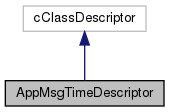
\includegraphics[width=199pt]{class_app_msg_time_descriptor__inherit__graph}
\end{center}
\end{figure}


Collaboration diagram for App\+Msg\+Time\+Descriptor\+:\nopagebreak
\begin{figure}[H]
\begin{center}
\leavevmode
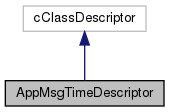
\includegraphics[width=199pt]{class_app_msg_time_descriptor__coll__graph}
\end{center}
\end{figure}
\subsection*{Public Member Functions}
\begin{DoxyCompactItemize}
\item 
\hyperlink{class_app_msg_time_descriptor_aa1c0a48d43a21f17d556759173b321b5}{App\+Msg\+Time\+Descriptor} ()
\item 
virtual \hyperlink{class_app_msg_time_descriptor_a3ffd811d3278f9847f320937f8dc3767}{$\sim$\+App\+Msg\+Time\+Descriptor} ()
\item 
virtual bool \hyperlink{class_app_msg_time_descriptor_a97ef37da3e4190f8e45a0ce2ee871e18}{does\+Support} (omnetpp\+::c\+Object $\ast$obj) const override
\item 
virtual const char $\ast$$\ast$ \hyperlink{class_app_msg_time_descriptor_a88a8a3b34a9af1d9a73c6601969cc5fc}{get\+Property\+Names} () const override
\item 
virtual const char $\ast$ \hyperlink{class_app_msg_time_descriptor_ab9f6a79300cffb71dda8372c3c4bef83}{get\+Property} (const char $\ast$propertyname) const override
\item 
virtual int \hyperlink{class_app_msg_time_descriptor_a754ebbbce52e3b7bfe97a0aef282b3a3}{get\+Field\+Count} () const override
\item 
virtual const char $\ast$ \hyperlink{class_app_msg_time_descriptor_ac986a70c33fc35e90bdf543c6b4d2fe4}{get\+Field\+Name} (int field) const override
\item 
virtual int \hyperlink{class_app_msg_time_descriptor_a18f5251d319288bc3b893b1186b7777f}{find\+Field} (const char $\ast$field\+Name) const override
\item 
virtual unsigned int \hyperlink{class_app_msg_time_descriptor_a9c4f1ee9ba789821e48b7cf0e4be6511}{get\+Field\+Type\+Flags} (int field) const override
\item 
virtual const char $\ast$ \hyperlink{class_app_msg_time_descriptor_a576cceeffd841b561c7c8f9bb92fff85}{get\+Field\+Type\+String} (int field) const override
\item 
virtual const char $\ast$$\ast$ \hyperlink{class_app_msg_time_descriptor_adbedb4b0c116a04c4fb28bf1d6875e79}{get\+Field\+Property\+Names} (int field) const override
\item 
virtual const char $\ast$ \hyperlink{class_app_msg_time_descriptor_afabdeba686e7822bf682e81b6ee7009d}{get\+Field\+Property} (int field, const char $\ast$propertyname) const override
\item 
virtual int \hyperlink{class_app_msg_time_descriptor_a57eb5d1436a72fc03d674e70cf46af7e}{get\+Field\+Array\+Size} (void $\ast$object, int field) const override
\item 
virtual const char $\ast$ \hyperlink{class_app_msg_time_descriptor_a8e410f5a62c300aae0066bc7c979d953}{get\+Field\+Dynamic\+Type\+String} (void $\ast$object, int field, int i) const override
\item 
virtual std\+::string \hyperlink{class_app_msg_time_descriptor_adfd92cca9d3fdd2705e303d1f5121c07}{get\+Field\+Value\+As\+String} (void $\ast$object, int field, int i) const override
\item 
virtual bool \hyperlink{class_app_msg_time_descriptor_abb26d4a890c0ec9753b49970adfd597c}{set\+Field\+Value\+As\+String} (void $\ast$object, int field, int i, const char $\ast$value) const override
\item 
virtual const char $\ast$ \hyperlink{class_app_msg_time_descriptor_a0b91efc1f981d4594f4361e9dab2dd49}{get\+Field\+Struct\+Name} (int field) const override
\item 
virtual void $\ast$ \hyperlink{class_app_msg_time_descriptor_a974b4e6fe474d1a56870c30030efe18d}{get\+Field\+Struct\+Value\+Pointer} (void $\ast$object, int field, int i) const override
\end{DoxyCompactItemize}
\subsection*{Private Attributes}
\begin{DoxyCompactItemize}
\item 
const char $\ast$$\ast$ \hyperlink{class_app_msg_time_descriptor_a102cbf09a1ba7e40df81cca8c3c503b4}{propertynames}
\end{DoxyCompactItemize}


\subsection{Constructor \& Destructor Documentation}
\mbox{\Hypertarget{class_app_msg_time_descriptor_aa1c0a48d43a21f17d556759173b321b5}\label{class_app_msg_time_descriptor_aa1c0a48d43a21f17d556759173b321b5}} 
\index{App\+Msg\+Time\+Descriptor@{App\+Msg\+Time\+Descriptor}!App\+Msg\+Time\+Descriptor@{App\+Msg\+Time\+Descriptor}}
\index{App\+Msg\+Time\+Descriptor@{App\+Msg\+Time\+Descriptor}!App\+Msg\+Time\+Descriptor@{App\+Msg\+Time\+Descriptor}}
\subsubsection{\texorpdfstring{App\+Msg\+Time\+Descriptor()}{AppMsgTimeDescriptor()}}
{\footnotesize\ttfamily App\+Msg\+Time\+Descriptor\+::\+App\+Msg\+Time\+Descriptor (\begin{DoxyParamCaption}{ }\end{DoxyParamCaption})}

\mbox{\Hypertarget{class_app_msg_time_descriptor_a3ffd811d3278f9847f320937f8dc3767}\label{class_app_msg_time_descriptor_a3ffd811d3278f9847f320937f8dc3767}} 
\index{App\+Msg\+Time\+Descriptor@{App\+Msg\+Time\+Descriptor}!````~App\+Msg\+Time\+Descriptor@{$\sim$\+App\+Msg\+Time\+Descriptor}}
\index{````~App\+Msg\+Time\+Descriptor@{$\sim$\+App\+Msg\+Time\+Descriptor}!App\+Msg\+Time\+Descriptor@{App\+Msg\+Time\+Descriptor}}
\subsubsection{\texorpdfstring{$\sim$\+App\+Msg\+Time\+Descriptor()}{~AppMsgTimeDescriptor()}}
{\footnotesize\ttfamily App\+Msg\+Time\+Descriptor\+::$\sim$\+App\+Msg\+Time\+Descriptor (\begin{DoxyParamCaption}{ }\end{DoxyParamCaption})\hspace{0.3cm}{\ttfamily [virtual]}}



\subsection{Member Function Documentation}
\mbox{\Hypertarget{class_app_msg_time_descriptor_a97ef37da3e4190f8e45a0ce2ee871e18}\label{class_app_msg_time_descriptor_a97ef37da3e4190f8e45a0ce2ee871e18}} 
\index{App\+Msg\+Time\+Descriptor@{App\+Msg\+Time\+Descriptor}!does\+Support@{does\+Support}}
\index{does\+Support@{does\+Support}!App\+Msg\+Time\+Descriptor@{App\+Msg\+Time\+Descriptor}}
\subsubsection{\texorpdfstring{does\+Support()}{doesSupport()}}
{\footnotesize\ttfamily bool App\+Msg\+Time\+Descriptor\+::does\+Support (\begin{DoxyParamCaption}\item[{omnetpp\+::c\+Object $\ast$}]{obj }\end{DoxyParamCaption}) const\hspace{0.3cm}{\ttfamily [override]}, {\ttfamily [virtual]}}

\mbox{\Hypertarget{class_app_msg_time_descriptor_a18f5251d319288bc3b893b1186b7777f}\label{class_app_msg_time_descriptor_a18f5251d319288bc3b893b1186b7777f}} 
\index{App\+Msg\+Time\+Descriptor@{App\+Msg\+Time\+Descriptor}!find\+Field@{find\+Field}}
\index{find\+Field@{find\+Field}!App\+Msg\+Time\+Descriptor@{App\+Msg\+Time\+Descriptor}}
\subsubsection{\texorpdfstring{find\+Field()}{findField()}}
{\footnotesize\ttfamily int App\+Msg\+Time\+Descriptor\+::find\+Field (\begin{DoxyParamCaption}\item[{const char $\ast$}]{field\+Name }\end{DoxyParamCaption}) const\hspace{0.3cm}{\ttfamily [override]}, {\ttfamily [virtual]}}

\mbox{\Hypertarget{class_app_msg_time_descriptor_a57eb5d1436a72fc03d674e70cf46af7e}\label{class_app_msg_time_descriptor_a57eb5d1436a72fc03d674e70cf46af7e}} 
\index{App\+Msg\+Time\+Descriptor@{App\+Msg\+Time\+Descriptor}!get\+Field\+Array\+Size@{get\+Field\+Array\+Size}}
\index{get\+Field\+Array\+Size@{get\+Field\+Array\+Size}!App\+Msg\+Time\+Descriptor@{App\+Msg\+Time\+Descriptor}}
\subsubsection{\texorpdfstring{get\+Field\+Array\+Size()}{getFieldArraySize()}}
{\footnotesize\ttfamily int App\+Msg\+Time\+Descriptor\+::get\+Field\+Array\+Size (\begin{DoxyParamCaption}\item[{void $\ast$}]{object,  }\item[{int}]{field }\end{DoxyParamCaption}) const\hspace{0.3cm}{\ttfamily [override]}, {\ttfamily [virtual]}}

\mbox{\Hypertarget{class_app_msg_time_descriptor_a754ebbbce52e3b7bfe97a0aef282b3a3}\label{class_app_msg_time_descriptor_a754ebbbce52e3b7bfe97a0aef282b3a3}} 
\index{App\+Msg\+Time\+Descriptor@{App\+Msg\+Time\+Descriptor}!get\+Field\+Count@{get\+Field\+Count}}
\index{get\+Field\+Count@{get\+Field\+Count}!App\+Msg\+Time\+Descriptor@{App\+Msg\+Time\+Descriptor}}
\subsubsection{\texorpdfstring{get\+Field\+Count()}{getFieldCount()}}
{\footnotesize\ttfamily int App\+Msg\+Time\+Descriptor\+::get\+Field\+Count (\begin{DoxyParamCaption}{ }\end{DoxyParamCaption}) const\hspace{0.3cm}{\ttfamily [override]}, {\ttfamily [virtual]}}

\mbox{\Hypertarget{class_app_msg_time_descriptor_a8e410f5a62c300aae0066bc7c979d953}\label{class_app_msg_time_descriptor_a8e410f5a62c300aae0066bc7c979d953}} 
\index{App\+Msg\+Time\+Descriptor@{App\+Msg\+Time\+Descriptor}!get\+Field\+Dynamic\+Type\+String@{get\+Field\+Dynamic\+Type\+String}}
\index{get\+Field\+Dynamic\+Type\+String@{get\+Field\+Dynamic\+Type\+String}!App\+Msg\+Time\+Descriptor@{App\+Msg\+Time\+Descriptor}}
\subsubsection{\texorpdfstring{get\+Field\+Dynamic\+Type\+String()}{getFieldDynamicTypeString()}}
{\footnotesize\ttfamily const char $\ast$ App\+Msg\+Time\+Descriptor\+::get\+Field\+Dynamic\+Type\+String (\begin{DoxyParamCaption}\item[{void $\ast$}]{object,  }\item[{int}]{field,  }\item[{int}]{i }\end{DoxyParamCaption}) const\hspace{0.3cm}{\ttfamily [override]}, {\ttfamily [virtual]}}

\mbox{\Hypertarget{class_app_msg_time_descriptor_ac986a70c33fc35e90bdf543c6b4d2fe4}\label{class_app_msg_time_descriptor_ac986a70c33fc35e90bdf543c6b4d2fe4}} 
\index{App\+Msg\+Time\+Descriptor@{App\+Msg\+Time\+Descriptor}!get\+Field\+Name@{get\+Field\+Name}}
\index{get\+Field\+Name@{get\+Field\+Name}!App\+Msg\+Time\+Descriptor@{App\+Msg\+Time\+Descriptor}}
\subsubsection{\texorpdfstring{get\+Field\+Name()}{getFieldName()}}
{\footnotesize\ttfamily const char $\ast$ App\+Msg\+Time\+Descriptor\+::get\+Field\+Name (\begin{DoxyParamCaption}\item[{int}]{field }\end{DoxyParamCaption}) const\hspace{0.3cm}{\ttfamily [override]}, {\ttfamily [virtual]}}

\mbox{\Hypertarget{class_app_msg_time_descriptor_afabdeba686e7822bf682e81b6ee7009d}\label{class_app_msg_time_descriptor_afabdeba686e7822bf682e81b6ee7009d}} 
\index{App\+Msg\+Time\+Descriptor@{App\+Msg\+Time\+Descriptor}!get\+Field\+Property@{get\+Field\+Property}}
\index{get\+Field\+Property@{get\+Field\+Property}!App\+Msg\+Time\+Descriptor@{App\+Msg\+Time\+Descriptor}}
\subsubsection{\texorpdfstring{get\+Field\+Property()}{getFieldProperty()}}
{\footnotesize\ttfamily const char $\ast$ App\+Msg\+Time\+Descriptor\+::get\+Field\+Property (\begin{DoxyParamCaption}\item[{int}]{field,  }\item[{const char $\ast$}]{propertyname }\end{DoxyParamCaption}) const\hspace{0.3cm}{\ttfamily [override]}, {\ttfamily [virtual]}}

\mbox{\Hypertarget{class_app_msg_time_descriptor_adbedb4b0c116a04c4fb28bf1d6875e79}\label{class_app_msg_time_descriptor_adbedb4b0c116a04c4fb28bf1d6875e79}} 
\index{App\+Msg\+Time\+Descriptor@{App\+Msg\+Time\+Descriptor}!get\+Field\+Property\+Names@{get\+Field\+Property\+Names}}
\index{get\+Field\+Property\+Names@{get\+Field\+Property\+Names}!App\+Msg\+Time\+Descriptor@{App\+Msg\+Time\+Descriptor}}
\subsubsection{\texorpdfstring{get\+Field\+Property\+Names()}{getFieldPropertyNames()}}
{\footnotesize\ttfamily const char $\ast$$\ast$ App\+Msg\+Time\+Descriptor\+::get\+Field\+Property\+Names (\begin{DoxyParamCaption}\item[{int}]{field }\end{DoxyParamCaption}) const\hspace{0.3cm}{\ttfamily [override]}, {\ttfamily [virtual]}}

\mbox{\Hypertarget{class_app_msg_time_descriptor_a0b91efc1f981d4594f4361e9dab2dd49}\label{class_app_msg_time_descriptor_a0b91efc1f981d4594f4361e9dab2dd49}} 
\index{App\+Msg\+Time\+Descriptor@{App\+Msg\+Time\+Descriptor}!get\+Field\+Struct\+Name@{get\+Field\+Struct\+Name}}
\index{get\+Field\+Struct\+Name@{get\+Field\+Struct\+Name}!App\+Msg\+Time\+Descriptor@{App\+Msg\+Time\+Descriptor}}
\subsubsection{\texorpdfstring{get\+Field\+Struct\+Name()}{getFieldStructName()}}
{\footnotesize\ttfamily const char $\ast$ App\+Msg\+Time\+Descriptor\+::get\+Field\+Struct\+Name (\begin{DoxyParamCaption}\item[{int}]{field }\end{DoxyParamCaption}) const\hspace{0.3cm}{\ttfamily [override]}, {\ttfamily [virtual]}}

\mbox{\Hypertarget{class_app_msg_time_descriptor_a974b4e6fe474d1a56870c30030efe18d}\label{class_app_msg_time_descriptor_a974b4e6fe474d1a56870c30030efe18d}} 
\index{App\+Msg\+Time\+Descriptor@{App\+Msg\+Time\+Descriptor}!get\+Field\+Struct\+Value\+Pointer@{get\+Field\+Struct\+Value\+Pointer}}
\index{get\+Field\+Struct\+Value\+Pointer@{get\+Field\+Struct\+Value\+Pointer}!App\+Msg\+Time\+Descriptor@{App\+Msg\+Time\+Descriptor}}
\subsubsection{\texorpdfstring{get\+Field\+Struct\+Value\+Pointer()}{getFieldStructValuePointer()}}
{\footnotesize\ttfamily void $\ast$ App\+Msg\+Time\+Descriptor\+::get\+Field\+Struct\+Value\+Pointer (\begin{DoxyParamCaption}\item[{void $\ast$}]{object,  }\item[{int}]{field,  }\item[{int}]{i }\end{DoxyParamCaption}) const\hspace{0.3cm}{\ttfamily [override]}, {\ttfamily [virtual]}}

\mbox{\Hypertarget{class_app_msg_time_descriptor_a9c4f1ee9ba789821e48b7cf0e4be6511}\label{class_app_msg_time_descriptor_a9c4f1ee9ba789821e48b7cf0e4be6511}} 
\index{App\+Msg\+Time\+Descriptor@{App\+Msg\+Time\+Descriptor}!get\+Field\+Type\+Flags@{get\+Field\+Type\+Flags}}
\index{get\+Field\+Type\+Flags@{get\+Field\+Type\+Flags}!App\+Msg\+Time\+Descriptor@{App\+Msg\+Time\+Descriptor}}
\subsubsection{\texorpdfstring{get\+Field\+Type\+Flags()}{getFieldTypeFlags()}}
{\footnotesize\ttfamily unsigned int App\+Msg\+Time\+Descriptor\+::get\+Field\+Type\+Flags (\begin{DoxyParamCaption}\item[{int}]{field }\end{DoxyParamCaption}) const\hspace{0.3cm}{\ttfamily [override]}, {\ttfamily [virtual]}}

\mbox{\Hypertarget{class_app_msg_time_descriptor_a576cceeffd841b561c7c8f9bb92fff85}\label{class_app_msg_time_descriptor_a576cceeffd841b561c7c8f9bb92fff85}} 
\index{App\+Msg\+Time\+Descriptor@{App\+Msg\+Time\+Descriptor}!get\+Field\+Type\+String@{get\+Field\+Type\+String}}
\index{get\+Field\+Type\+String@{get\+Field\+Type\+String}!App\+Msg\+Time\+Descriptor@{App\+Msg\+Time\+Descriptor}}
\subsubsection{\texorpdfstring{get\+Field\+Type\+String()}{getFieldTypeString()}}
{\footnotesize\ttfamily const char $\ast$ App\+Msg\+Time\+Descriptor\+::get\+Field\+Type\+String (\begin{DoxyParamCaption}\item[{int}]{field }\end{DoxyParamCaption}) const\hspace{0.3cm}{\ttfamily [override]}, {\ttfamily [virtual]}}

\mbox{\Hypertarget{class_app_msg_time_descriptor_adfd92cca9d3fdd2705e303d1f5121c07}\label{class_app_msg_time_descriptor_adfd92cca9d3fdd2705e303d1f5121c07}} 
\index{App\+Msg\+Time\+Descriptor@{App\+Msg\+Time\+Descriptor}!get\+Field\+Value\+As\+String@{get\+Field\+Value\+As\+String}}
\index{get\+Field\+Value\+As\+String@{get\+Field\+Value\+As\+String}!App\+Msg\+Time\+Descriptor@{App\+Msg\+Time\+Descriptor}}
\subsubsection{\texorpdfstring{get\+Field\+Value\+As\+String()}{getFieldValueAsString()}}
{\footnotesize\ttfamily std\+::string App\+Msg\+Time\+Descriptor\+::get\+Field\+Value\+As\+String (\begin{DoxyParamCaption}\item[{void $\ast$}]{object,  }\item[{int}]{field,  }\item[{int}]{i }\end{DoxyParamCaption}) const\hspace{0.3cm}{\ttfamily [override]}, {\ttfamily [virtual]}}

\mbox{\Hypertarget{class_app_msg_time_descriptor_ab9f6a79300cffb71dda8372c3c4bef83}\label{class_app_msg_time_descriptor_ab9f6a79300cffb71dda8372c3c4bef83}} 
\index{App\+Msg\+Time\+Descriptor@{App\+Msg\+Time\+Descriptor}!get\+Property@{get\+Property}}
\index{get\+Property@{get\+Property}!App\+Msg\+Time\+Descriptor@{App\+Msg\+Time\+Descriptor}}
\subsubsection{\texorpdfstring{get\+Property()}{getProperty()}}
{\footnotesize\ttfamily const char $\ast$ App\+Msg\+Time\+Descriptor\+::get\+Property (\begin{DoxyParamCaption}\item[{const char $\ast$}]{propertyname }\end{DoxyParamCaption}) const\hspace{0.3cm}{\ttfamily [override]}, {\ttfamily [virtual]}}

\mbox{\Hypertarget{class_app_msg_time_descriptor_a88a8a3b34a9af1d9a73c6601969cc5fc}\label{class_app_msg_time_descriptor_a88a8a3b34a9af1d9a73c6601969cc5fc}} 
\index{App\+Msg\+Time\+Descriptor@{App\+Msg\+Time\+Descriptor}!get\+Property\+Names@{get\+Property\+Names}}
\index{get\+Property\+Names@{get\+Property\+Names}!App\+Msg\+Time\+Descriptor@{App\+Msg\+Time\+Descriptor}}
\subsubsection{\texorpdfstring{get\+Property\+Names()}{getPropertyNames()}}
{\footnotesize\ttfamily const char $\ast$$\ast$ App\+Msg\+Time\+Descriptor\+::get\+Property\+Names (\begin{DoxyParamCaption}{ }\end{DoxyParamCaption}) const\hspace{0.3cm}{\ttfamily [override]}, {\ttfamily [virtual]}}

\mbox{\Hypertarget{class_app_msg_time_descriptor_abb26d4a890c0ec9753b49970adfd597c}\label{class_app_msg_time_descriptor_abb26d4a890c0ec9753b49970adfd597c}} 
\index{App\+Msg\+Time\+Descriptor@{App\+Msg\+Time\+Descriptor}!set\+Field\+Value\+As\+String@{set\+Field\+Value\+As\+String}}
\index{set\+Field\+Value\+As\+String@{set\+Field\+Value\+As\+String}!App\+Msg\+Time\+Descriptor@{App\+Msg\+Time\+Descriptor}}
\subsubsection{\texorpdfstring{set\+Field\+Value\+As\+String()}{setFieldValueAsString()}}
{\footnotesize\ttfamily bool App\+Msg\+Time\+Descriptor\+::set\+Field\+Value\+As\+String (\begin{DoxyParamCaption}\item[{void $\ast$}]{object,  }\item[{int}]{field,  }\item[{int}]{i,  }\item[{const char $\ast$}]{value }\end{DoxyParamCaption}) const\hspace{0.3cm}{\ttfamily [override]}, {\ttfamily [virtual]}}



\subsection{Member Data Documentation}
\mbox{\Hypertarget{class_app_msg_time_descriptor_a102cbf09a1ba7e40df81cca8c3c503b4}\label{class_app_msg_time_descriptor_a102cbf09a1ba7e40df81cca8c3c503b4}} 
\index{App\+Msg\+Time\+Descriptor@{App\+Msg\+Time\+Descriptor}!propertynames@{propertynames}}
\index{propertynames@{propertynames}!App\+Msg\+Time\+Descriptor@{App\+Msg\+Time\+Descriptor}}
\subsubsection{\texorpdfstring{propertynames}{propertynames}}
{\footnotesize\ttfamily const char$\ast$$\ast$ App\+Msg\+Time\+Descriptor\+::propertynames\hspace{0.3cm}{\ttfamily [mutable]}, {\ttfamily [private]}}



The documentation for this class was generated from the following file\+:\begin{DoxyCompactItemize}
\item 
src/\+Messages/\hyperlink{_app_msg__m_8cc}{App\+Msg\+\_\+m.\+cc}\end{DoxyCompactItemize}

\hypertarget{class_communication_dispatcher}{}\section{Communication\+Dispatcher Class Reference}
\label{class_communication_dispatcher}\index{Communication\+Dispatcher@{Communication\+Dispatcher}}


{\ttfamily \#include $<$communication\+Dispatcher.\+h$>$}



Inheritance diagram for Communication\+Dispatcher\+:\nopagebreak
\begin{figure}[H]
\begin{center}
\leavevmode
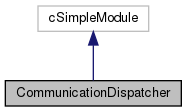
\includegraphics[width=212pt]{class_communication_dispatcher__inherit__graph}
\end{center}
\end{figure}


Collaboration diagram for Communication\+Dispatcher\+:\nopagebreak
\begin{figure}[H]
\begin{center}
\leavevmode
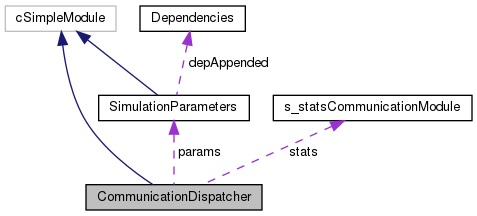
\includegraphics[width=350pt]{class_communication_dispatcher__coll__graph}
\end{center}
\end{figure}
\subsection*{Classes}
\begin{DoxyCompactItemize}
\item 
class \hyperlink{class_communication_dispatcher_1_1h}{h}
\begin{DoxyCompactList}\small\item\em Class used to connect nodes. \end{DoxyCompactList}\end{DoxyCompactItemize}
\subsection*{Private Member Functions}
\begin{DoxyCompactItemize}
\item 
virtual void \hyperlink{class_communication_dispatcher_ab44887658841bb5ab59c554c1738c8f3}{initialize} ()
\begin{DoxyCompactList}\small\item\em Initializes the communication\+Dispatcher. \end{DoxyCompactList}\item 
virtual void \hyperlink{class_communication_dispatcher_af7be3dbf46282e78d41d3d194f5ff246}{handle\+Message} (c\+Message $\ast$\hyperlink{_controller_8h_afa0f3b802fbc219228f7bb97996fa558}{msg})
\begin{DoxyCompactList}\small\item\em handles messages to forward \end{DoxyCompactList}\item 
void \hyperlink{class_communication_dispatcher_a589821f510801091f753f9812e3d1ee7}{broadcast\+App\+Message} (\hyperlink{class_app_msg}{App\+Msg} $\ast$m)
\begin{DoxyCompactList}\small\item\em Broadcasts an application message to all nodes. \end{DoxyCompactList}\item 
simtime\+\_\+t \hyperlink{class_communication_dispatcher_acf6f743d35e72c71d61275ad25cdc306}{compute\+Delay} (unsigned int id\+Source\+Process, unsigned int id\+Target\+Process)
\begin{DoxyCompactList}\small\item\em Computes the propagation delay of a message following the node id of the source and target processes. \end{DoxyCompactList}\item 
void \hyperlink{class_communication_dispatcher_ab87c3d69a5953f9bda369d53c2de90d7}{increment\+Delay\+Intervals} (unsigned int entry)
\begin{DoxyCompactList}\small\item\em Takes statistics of the propagation delay interval. \end{DoxyCompactList}\end{DoxyCompactItemize}
\subsection*{Private Attributes}
\begin{DoxyCompactItemize}
\item 
vector$<$ c\+Gate $\ast$ $>$ \hyperlink{class_communication_dispatcher_adf9f3838d1a7310757886421bb0e5bf7}{gates}
\begin{DoxyCompactList}\small\item\em vector containing a gate reference to each node. \end{DoxyCompactList}\item 
std\+::default\+\_\+random\+\_\+engine \hyperlink{class_communication_dispatcher_a9272f7c52493b1d2ac49c0954174ed1f}{generator\+Channel\+Delay}
\begin{DoxyCompactList}\small\item\em Used to generate channel propagation delays. \end{DoxyCompactList}\item 
std\+::normal\+\_\+distribution$<$ double $>$ \hyperlink{class_communication_dispatcher_a2505530ff3016939eef2ce9005847db1}{distribution\+Channel\+Delay\+Pair} = std\+::normal\+\_\+distribution$<$double$>$(\hyperlink{structures_8h_aa2bfff4413d2bdefb6cb5b708a31660b}{C\+H\+A\+N\+N\+E\+L\+D\+E\+L\+AY},30000.)
\item 
std\+::normal\+\_\+distribution$<$ double $>$ \hyperlink{class_communication_dispatcher_a12848fe0cdce112381265d7c4ba5d62a}{distribution\+Channel\+Delay\+Impair} = std\+::normal\+\_\+distribution$<$double$>$(\hyperlink{structures_8h_aa2bfff4413d2bdefb6cb5b708a31660b}{C\+H\+A\+N\+N\+E\+L\+D\+E\+L\+AY},30000.)
\item 
vector$<$ int $>$ \hyperlink{class_communication_dispatcher_acd67954c5bf9280a33d069ae4b217e1c}{channel\+Rand\+Number}
\begin{DoxyCompactList}\small\item\em Used to attribute a different channel number to each gate. \end{DoxyCompactList}\item 
\hyperlink{communication_dispatcher_8h_a9d0242025c5ba7fecd1b0c41f4777c06}{stats\+Communication\+Module} \hyperlink{class_communication_dispatcher_a5e01e95460682f3a31417efab24b25e4}{stats}
\begin{DoxyCompactList}\small\item\em \hyperlink{class_stats}{Stats} module to take statistics about message propagation delays. \end{DoxyCompactList}\item 
\hyperlink{class_simulation_parameters}{Simulation\+Parameters} $\ast$ \hyperlink{class_communication_dispatcher_a53751662d1e770a60ddbeea9d4a5d845}{params}
\begin{DoxyCompactList}\small\item\em Reference to the \hyperlink{class_simulation_parameters}{Simulation\+Parameters} module which contains the simulation parameters. \end{DoxyCompactList}\end{DoxyCompactItemize}


\subsection{Member Function Documentation}
\mbox{\Hypertarget{class_communication_dispatcher_a589821f510801091f753f9812e3d1ee7}\label{class_communication_dispatcher_a589821f510801091f753f9812e3d1ee7}} 
\index{Communication\+Dispatcher@{Communication\+Dispatcher}!broadcast\+App\+Message@{broadcast\+App\+Message}}
\index{broadcast\+App\+Message@{broadcast\+App\+Message}!Communication\+Dispatcher@{Communication\+Dispatcher}}
\subsubsection{\texorpdfstring{broadcast\+App\+Message()}{broadcastAppMessage()}}
{\footnotesize\ttfamily void Communication\+Dispatcher\+::broadcast\+App\+Message (\begin{DoxyParamCaption}\item[{\hyperlink{class_app_msg}{App\+Msg} $\ast$}]{m }\end{DoxyParamCaption})\hspace{0.3cm}{\ttfamily [private]}}



Broadcasts an application message to all nodes. 


\begin{DoxyParams}{Parameters}
{\em m} & Message to broadcast \\
\hline
\end{DoxyParams}
\mbox{\Hypertarget{class_communication_dispatcher_acf6f743d35e72c71d61275ad25cdc306}\label{class_communication_dispatcher_acf6f743d35e72c71d61275ad25cdc306}} 
\index{Communication\+Dispatcher@{Communication\+Dispatcher}!compute\+Delay@{compute\+Delay}}
\index{compute\+Delay@{compute\+Delay}!Communication\+Dispatcher@{Communication\+Dispatcher}}
\subsubsection{\texorpdfstring{compute\+Delay()}{computeDelay()}}
{\footnotesize\ttfamily simtime\+\_\+t Communication\+Dispatcher\+::compute\+Delay (\begin{DoxyParamCaption}\item[{unsigned int}]{id\+Source\+Process,  }\item[{unsigned int}]{id\+Target\+Process }\end{DoxyParamCaption})\hspace{0.3cm}{\ttfamily [private]}}



Computes the propagation delay of a message following the node id of the source and target processes. 


\begin{DoxyParams}{Parameters}
{\em id\+Source\+Process} & node id of the process that sent the message \\
\hline
{\em id\+Target\+Process} & node id of the destination process of the message \\
\hline
\end{DoxyParams}
\begin{DoxyReturn}{Returns}
message propagation delay 
\end{DoxyReturn}
\mbox{\Hypertarget{class_communication_dispatcher_af7be3dbf46282e78d41d3d194f5ff246}\label{class_communication_dispatcher_af7be3dbf46282e78d41d3d194f5ff246}} 
\index{Communication\+Dispatcher@{Communication\+Dispatcher}!handle\+Message@{handle\+Message}}
\index{handle\+Message@{handle\+Message}!Communication\+Dispatcher@{Communication\+Dispatcher}}
\subsubsection{\texorpdfstring{handle\+Message()}{handleMessage()}}
{\footnotesize\ttfamily void Communication\+Dispatcher\+::handle\+Message (\begin{DoxyParamCaption}\item[{c\+Message $\ast$}]{msg }\end{DoxyParamCaption})\hspace{0.3cm}{\ttfamily [private]}, {\ttfamily [virtual]}}



handles messages to forward 


\begin{DoxyParams}{Parameters}
{\em msg} & Message to forward \\
\hline
\end{DoxyParams}
\mbox{\Hypertarget{class_communication_dispatcher_ab87c3d69a5953f9bda369d53c2de90d7}\label{class_communication_dispatcher_ab87c3d69a5953f9bda369d53c2de90d7}} 
\index{Communication\+Dispatcher@{Communication\+Dispatcher}!increment\+Delay\+Intervals@{increment\+Delay\+Intervals}}
\index{increment\+Delay\+Intervals@{increment\+Delay\+Intervals}!Communication\+Dispatcher@{Communication\+Dispatcher}}
\subsubsection{\texorpdfstring{increment\+Delay\+Intervals()}{incrementDelayIntervals()}}
{\footnotesize\ttfamily void Communication\+Dispatcher\+::increment\+Delay\+Intervals (\begin{DoxyParamCaption}\item[{unsigned int}]{entry }\end{DoxyParamCaption})\hspace{0.3cm}{\ttfamily [private]}}



Takes statistics of the propagation delay interval. 


\begin{DoxyParams}{Parameters}
{\em entry} & propagation interval to increment \\
\hline
\end{DoxyParams}
\mbox{\Hypertarget{class_communication_dispatcher_ab44887658841bb5ab59c554c1738c8f3}\label{class_communication_dispatcher_ab44887658841bb5ab59c554c1738c8f3}} 
\index{Communication\+Dispatcher@{Communication\+Dispatcher}!initialize@{initialize}}
\index{initialize@{initialize}!Communication\+Dispatcher@{Communication\+Dispatcher}}
\subsubsection{\texorpdfstring{initialize()}{initialize()}}
{\footnotesize\ttfamily void Communication\+Dispatcher\+::initialize (\begin{DoxyParamCaption}{ }\end{DoxyParamCaption})\hspace{0.3cm}{\ttfamily [private]}, {\ttfamily [virtual]}}



Initializes the communication\+Dispatcher. 



\subsection{Member Data Documentation}
\mbox{\Hypertarget{class_communication_dispatcher_acd67954c5bf9280a33d069ae4b217e1c}\label{class_communication_dispatcher_acd67954c5bf9280a33d069ae4b217e1c}} 
\index{Communication\+Dispatcher@{Communication\+Dispatcher}!channel\+Rand\+Number@{channel\+Rand\+Number}}
\index{channel\+Rand\+Number@{channel\+Rand\+Number}!Communication\+Dispatcher@{Communication\+Dispatcher}}
\subsubsection{\texorpdfstring{channel\+Rand\+Number}{channelRandNumber}}
{\footnotesize\ttfamily vector$<$int$>$ Communication\+Dispatcher\+::channel\+Rand\+Number\hspace{0.3cm}{\ttfamily [private]}}



Used to attribute a different channel number to each gate. 

\mbox{\Hypertarget{class_communication_dispatcher_a12848fe0cdce112381265d7c4ba5d62a}\label{class_communication_dispatcher_a12848fe0cdce112381265d7c4ba5d62a}} 
\index{Communication\+Dispatcher@{Communication\+Dispatcher}!distribution\+Channel\+Delay\+Impair@{distribution\+Channel\+Delay\+Impair}}
\index{distribution\+Channel\+Delay\+Impair@{distribution\+Channel\+Delay\+Impair}!Communication\+Dispatcher@{Communication\+Dispatcher}}
\subsubsection{\texorpdfstring{distribution\+Channel\+Delay\+Impair}{distributionChannelDelayImpair}}
{\footnotesize\ttfamily std\+::normal\+\_\+distribution$<$double$>$ Communication\+Dispatcher\+::distribution\+Channel\+Delay\+Impair = std\+::normal\+\_\+distribution$<$double$>$(\hyperlink{structures_8h_aa2bfff4413d2bdefb6cb5b708a31660b}{C\+H\+A\+N\+N\+E\+L\+D\+E\+L\+AY},30000.)\hspace{0.3cm}{\ttfamily [private]}}

\mbox{\Hypertarget{class_communication_dispatcher_a2505530ff3016939eef2ce9005847db1}\label{class_communication_dispatcher_a2505530ff3016939eef2ce9005847db1}} 
\index{Communication\+Dispatcher@{Communication\+Dispatcher}!distribution\+Channel\+Delay\+Pair@{distribution\+Channel\+Delay\+Pair}}
\index{distribution\+Channel\+Delay\+Pair@{distribution\+Channel\+Delay\+Pair}!Communication\+Dispatcher@{Communication\+Dispatcher}}
\subsubsection{\texorpdfstring{distribution\+Channel\+Delay\+Pair}{distributionChannelDelayPair}}
{\footnotesize\ttfamily std\+::normal\+\_\+distribution$<$double$>$ Communication\+Dispatcher\+::distribution\+Channel\+Delay\+Pair = std\+::normal\+\_\+distribution$<$double$>$(\hyperlink{structures_8h_aa2bfff4413d2bdefb6cb5b708a31660b}{C\+H\+A\+N\+N\+E\+L\+D\+E\+L\+AY},30000.)\hspace{0.3cm}{\ttfamily [private]}}

\mbox{\Hypertarget{class_communication_dispatcher_adf9f3838d1a7310757886421bb0e5bf7}\label{class_communication_dispatcher_adf9f3838d1a7310757886421bb0e5bf7}} 
\index{Communication\+Dispatcher@{Communication\+Dispatcher}!gates@{gates}}
\index{gates@{gates}!Communication\+Dispatcher@{Communication\+Dispatcher}}
\subsubsection{\texorpdfstring{gates}{gates}}
{\footnotesize\ttfamily vector$<$c\+Gate$\ast$$>$ Communication\+Dispatcher\+::gates\hspace{0.3cm}{\ttfamily [private]}}



vector containing a gate reference to each node. 

\mbox{\Hypertarget{class_communication_dispatcher_a9272f7c52493b1d2ac49c0954174ed1f}\label{class_communication_dispatcher_a9272f7c52493b1d2ac49c0954174ed1f}} 
\index{Communication\+Dispatcher@{Communication\+Dispatcher}!generator\+Channel\+Delay@{generator\+Channel\+Delay}}
\index{generator\+Channel\+Delay@{generator\+Channel\+Delay}!Communication\+Dispatcher@{Communication\+Dispatcher}}
\subsubsection{\texorpdfstring{generator\+Channel\+Delay}{generatorChannelDelay}}
{\footnotesize\ttfamily std\+::default\+\_\+random\+\_\+engine Communication\+Dispatcher\+::generator\+Channel\+Delay\hspace{0.3cm}{\ttfamily [private]}}



Used to generate channel propagation delays. 

\mbox{\Hypertarget{class_communication_dispatcher_a53751662d1e770a60ddbeea9d4a5d845}\label{class_communication_dispatcher_a53751662d1e770a60ddbeea9d4a5d845}} 
\index{Communication\+Dispatcher@{Communication\+Dispatcher}!params@{params}}
\index{params@{params}!Communication\+Dispatcher@{Communication\+Dispatcher}}
\subsubsection{\texorpdfstring{params}{params}}
{\footnotesize\ttfamily \hyperlink{class_simulation_parameters}{Simulation\+Parameters}$\ast$ Communication\+Dispatcher\+::params\hspace{0.3cm}{\ttfamily [private]}}



Reference to the \hyperlink{class_simulation_parameters}{Simulation\+Parameters} module which contains the simulation parameters. 

\mbox{\Hypertarget{class_communication_dispatcher_a5e01e95460682f3a31417efab24b25e4}\label{class_communication_dispatcher_a5e01e95460682f3a31417efab24b25e4}} 
\index{Communication\+Dispatcher@{Communication\+Dispatcher}!stats@{stats}}
\index{stats@{stats}!Communication\+Dispatcher@{Communication\+Dispatcher}}
\subsubsection{\texorpdfstring{stats}{stats}}
{\footnotesize\ttfamily \hyperlink{communication_dispatcher_8h_a9d0242025c5ba7fecd1b0c41f4777c06}{stats\+Communication\+Module} Communication\+Dispatcher\+::stats\hspace{0.3cm}{\ttfamily [private]}}



\hyperlink{class_stats}{Stats} module to take statistics about message propagation delays. 



The documentation for this class was generated from the following files\+:\begin{DoxyCompactItemize}
\item 
src/\hyperlink{communication_dispatcher_8h}{communication\+Dispatcher.\+h}\item 
src/\hyperlink{communication_dispatcher_8cc}{communication\+Dispatcher.\+cc}\end{DoxyCompactItemize}

\hypertarget{class_controller}{}\section{Controller Class Reference}
\label{class_controller}\index{Controller@{Controller}}


Module to control that nodes deliver application messages exactly once and in causal order.  




{\ttfamily \#include $<$Controller.\+h$>$}



Inheritance diagram for Controller\+:
\nopagebreak
\begin{figure}[H]
\begin{center}
\leavevmode
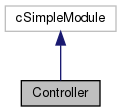
\includegraphics[width=163pt]{class_controller__inherit__graph}
\end{center}
\end{figure}


Collaboration diagram for Controller\+:
\nopagebreak
\begin{figure}[H]
\begin{center}
\leavevmode
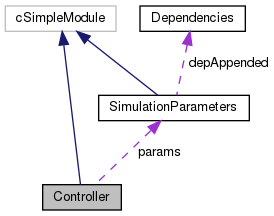
\includegraphics[width=278pt]{class_controller__coll__graph}
\end{center}
\end{figure}
\subsection*{Public Member Functions}
\begin{DoxyCompactItemize}
\item 
\hyperlink{class_controller_a95c56822d667e94b031451729ce069a9}{Controller} ()
\item 
virtual \hyperlink{class_controller_a0ab87934c4f7a266cfdb86e0f36bc1b5}{$\sim$\+Controller} ()
\item 
bool \hyperlink{class_controller_ad76a99df69bf99705dc18ba72b4b04c2}{is\+Dependency} (\hyperlink{structures_8h_a83a1d9a070efa5341da84cfd8e28d3e5}{id\+Msg} idM, \hyperlink{structures_8h_a83a1d9a070efa5341da84cfd8e28d3e5}{id\+Msg} id\+Dep)
\begin{DoxyCompactList}\small\item\em Checks if a message is a causal dependency of another message. \end{DoxyCompactList}\item 
void \hyperlink{class_controller_a7207304a07534e50a690f26c765b4a71}{notify\+Send\+Message} (unsigned int id\+Sender, unsigned int seq)
\begin{DoxyCompactList}\small\item\em Called by nodees when broadcasting a message to save the broadcasted message at the controller. \end{DoxyCompactList}\item 
bool \hyperlink{class_controller_a8905abf1976e737410ac0142001e38a0}{notify\+Deliver\+Message} (\hyperlink{structures_8h_a83a1d9a070efa5341da84cfd8e28d3e5}{id\+Msg} idM, unsigned int id\+Dest)
\begin{DoxyCompactList}\small\item\em Called by a node when delivering a message to notify the controller of the delivery, which verifies that the node delivers the message only once and in causal order. \end{DoxyCompactList}\item 
bool \hyperlink{class_controller_ab57c4459f002be63b4deda1d7c3c3e29}{can\+Causally\+Deliver\+Message} (\hyperlink{structures_8h_a83a1d9a070efa5341da84cfd8e28d3e5}{id\+Msg} idM, unsigned int id\+Dest)
\begin{DoxyCompactList}\small\item\em Verifies that a proces can causally deliver a message. \end{DoxyCompactList}\end{DoxyCompactItemize}
\subsection*{Private Member Functions}
\begin{DoxyCompactItemize}
\item 
virtual void \hyperlink{class_controller_a28d5755bc8fed07cebd88f857f0f83df}{initialize} ()
\begin{DoxyCompactList}\small\item\em Initializes the controller. \end{DoxyCompactList}\item 
vector$<$ \hyperlink{_controller_8h_afa0f3b802fbc219228f7bb97996fa558}{msg} $>$\+::iterator \hyperlink{class_controller_aa32d5c18e9e30caf2900527e42b93d44}{search\+Message} (\hyperlink{structures_8h_a83a1d9a070efa5341da84cfd8e28d3e5}{id\+Msg} idM)
\begin{DoxyCompactList}\small\item\em Searches the structure associated to a broadcasted message. \end{DoxyCompactList}\item 
void \hyperlink{class_controller_aa3c4ebef8d344e10e86c1b4f95171281}{print\+Delivery\+Error} (string error\+Reason, \hyperlink{structures_8h_a83a1d9a070efa5341da84cfd8e28d3e5}{id\+Msg} idM, unsigned int destnode, const \hyperlink{class_total_dependencies}{Total\+Dependencies} \&message\+Dependencies, const \hyperlink{class_total_dependencies}{Total\+Dependencies} \&\hyperlink{class_controller_ade3eeb8e78c5307d518e3b43967c4bac}{node\+Dependencies})
\begin{DoxyCompactList}\small\item\em Called to print delivery errors. \end{DoxyCompactList}\item 
void \hyperlink{class_controller_ab250759d5c511ceb8f35fdf9e42583cd}{delete\+Message} (\hyperlink{structures_8h_a83a1d9a070efa5341da84cfd8e28d3e5}{id\+Msg} idM)
\begin{DoxyCompactList}\small\item\em Called to remove messages delivered by all processes. \end{DoxyCompactList}\end{DoxyCompactItemize}
\subsection*{Private Attributes}
\begin{DoxyCompactItemize}
\item 
vector$<$ vector$<$ \hyperlink{_controller_8h_afa0f3b802fbc219228f7bb97996fa558}{msg} $>$ $>$ \hyperlink{class_controller_a4016e696420b0a6b14308b117070b506}{node\+Broadcasted\+Messages}
\begin{DoxyCompactList}\small\item\em Contains for each node \$p\+\_\+i\$ a structure per message that is currently broadcasted (not yet delivered by all nodes). \end{DoxyCompactList}\item 
vector$<$ \hyperlink{class_total_dependencies}{Total\+Dependencies} $>$ \hyperlink{class_controller_ade3eeb8e78c5307d518e3b43967c4bac}{node\+Dependencies}
\begin{DoxyCompactList}\small\item\em Contains the dependencies for each node. \end{DoxyCompactList}\item 
\hyperlink{class_simulation_parameters}{Simulation\+Parameters} $\ast$ \hyperlink{class_controller_a81d7fe43b78ef7601e6b36c3df38ce79}{params}
\begin{DoxyCompactList}\small\item\em Reference to the simulation parameters to avoid looking them up in each function. \end{DoxyCompactList}\end{DoxyCompactItemize}


\subsection{Detailed Description}
Module to control that nodes deliver application messages exactly once and in causal order. 

\subsection{Constructor \& Destructor Documentation}
\mbox{\Hypertarget{class_controller_a95c56822d667e94b031451729ce069a9}\label{class_controller_a95c56822d667e94b031451729ce069a9}} 
\index{Controller@{Controller}!Controller@{Controller}}
\index{Controller@{Controller}!Controller@{Controller}}
\subsubsection{\texorpdfstring{Controller()}{Controller()}}
{\footnotesize\ttfamily Controller\+::\+Controller (\begin{DoxyParamCaption}{ }\end{DoxyParamCaption})}

\mbox{\Hypertarget{class_controller_a0ab87934c4f7a266cfdb86e0f36bc1b5}\label{class_controller_a0ab87934c4f7a266cfdb86e0f36bc1b5}} 
\index{Controller@{Controller}!````~Controller@{$\sim$\+Controller}}
\index{````~Controller@{$\sim$\+Controller}!Controller@{Controller}}
\subsubsection{\texorpdfstring{$\sim$\+Controller()}{~Controller()}}
{\footnotesize\ttfamily Controller\+::$\sim$\+Controller (\begin{DoxyParamCaption}{ }\end{DoxyParamCaption})\hspace{0.3cm}{\ttfamily [virtual]}}



\subsection{Member Function Documentation}
\mbox{\Hypertarget{class_controller_ab57c4459f002be63b4deda1d7c3c3e29}\label{class_controller_ab57c4459f002be63b4deda1d7c3c3e29}} 
\index{Controller@{Controller}!can\+Causally\+Deliver\+Message@{can\+Causally\+Deliver\+Message}}
\index{can\+Causally\+Deliver\+Message@{can\+Causally\+Deliver\+Message}!Controller@{Controller}}
\subsubsection{\texorpdfstring{can\+Causally\+Deliver\+Message()}{canCausallyDeliverMessage()}}
{\footnotesize\ttfamily bool Controller\+::can\+Causally\+Deliver\+Message (\begin{DoxyParamCaption}\item[{\hyperlink{structures_8h_a83a1d9a070efa5341da84cfd8e28d3e5}{id\+Msg}}]{idM,  }\item[{unsigned int}]{id\+Dest }\end{DoxyParamCaption})}



Verifies that a proces can causally deliver a message. 


\begin{DoxyParams}{Parameters}
{\em idM} & The message to deliver. \\
\hline
{\em id\+Dest} & The process that will deliver the message. \\
\hline
\end{DoxyParams}
\begin{DoxyReturn}{Returns}
True if the process can deliver the message in causal order and false otherwise. 
\end{DoxyReturn}
\mbox{\Hypertarget{class_controller_ab250759d5c511ceb8f35fdf9e42583cd}\label{class_controller_ab250759d5c511ceb8f35fdf9e42583cd}} 
\index{Controller@{Controller}!delete\+Message@{delete\+Message}}
\index{delete\+Message@{delete\+Message}!Controller@{Controller}}
\subsubsection{\texorpdfstring{delete\+Message()}{deleteMessage()}}
{\footnotesize\ttfamily void Controller\+::delete\+Message (\begin{DoxyParamCaption}\item[{\hyperlink{structures_8h_a83a1d9a070efa5341da84cfd8e28d3e5}{id\+Msg}}]{idM }\end{DoxyParamCaption})\hspace{0.3cm}{\ttfamily [private]}}



Called to remove messages delivered by all processes. 

Raises an error if the message is not registered. 
\begin{DoxyParams}{Parameters}
{\em idM} & The message\textquotesingle{}s identificator. \\
\hline
\end{DoxyParams}
\mbox{\Hypertarget{class_controller_a28d5755bc8fed07cebd88f857f0f83df}\label{class_controller_a28d5755bc8fed07cebd88f857f0f83df}} 
\index{Controller@{Controller}!initialize@{initialize}}
\index{initialize@{initialize}!Controller@{Controller}}
\subsubsection{\texorpdfstring{initialize()}{initialize()}}
{\footnotesize\ttfamily void Controller\+::initialize (\begin{DoxyParamCaption}{ }\end{DoxyParamCaption})\hspace{0.3cm}{\ttfamily [private]}, {\ttfamily [virtual]}}



Initializes the controller. 

\mbox{\Hypertarget{class_controller_ad76a99df69bf99705dc18ba72b4b04c2}\label{class_controller_ad76a99df69bf99705dc18ba72b4b04c2}} 
\index{Controller@{Controller}!is\+Dependency@{is\+Dependency}}
\index{is\+Dependency@{is\+Dependency}!Controller@{Controller}}
\subsubsection{\texorpdfstring{is\+Dependency()}{isDependency()}}
{\footnotesize\ttfamily bool Controller\+::is\+Dependency (\begin{DoxyParamCaption}\item[{\hyperlink{structures_8h_a83a1d9a070efa5341da84cfd8e28d3e5}{id\+Msg}}]{idM,  }\item[{\hyperlink{structures_8h_a83a1d9a070efa5341da84cfd8e28d3e5}{id\+Msg}}]{id\+Dep }\end{DoxyParamCaption})}



Checks if a message is a causal dependency of another message. 


\begin{DoxyParams}{Parameters}
{\em idM} & Message of which wants to check the dependency. \\
\hline
{\em id\+Dep} & Dependency to be checked. \\
\hline
\end{DoxyParams}
\begin{DoxyReturn}{Returns}
true if id\+Dep is a dependency of idM and false otherwise. 
\end{DoxyReturn}
\mbox{\Hypertarget{class_controller_a8905abf1976e737410ac0142001e38a0}\label{class_controller_a8905abf1976e737410ac0142001e38a0}} 
\index{Controller@{Controller}!notify\+Deliver\+Message@{notify\+Deliver\+Message}}
\index{notify\+Deliver\+Message@{notify\+Deliver\+Message}!Controller@{Controller}}
\subsubsection{\texorpdfstring{notify\+Deliver\+Message()}{notifyDeliverMessage()}}
{\footnotesize\ttfamily bool Controller\+::notify\+Deliver\+Message (\begin{DoxyParamCaption}\item[{\hyperlink{structures_8h_a83a1d9a070efa5341da84cfd8e28d3e5}{id\+Msg}}]{idM,  }\item[{unsigned int}]{id\+Dest }\end{DoxyParamCaption})}



Called by a node when delivering a message to notify the controller of the delivery, which verifies that the node delivers the message only once and in causal order. 

The function exists if the node has already delivered the message. 
\begin{DoxyParams}{Parameters}
{\em idM} & the message\textquotesingle{}s identificator. \\
\hline
{\em id\+Dest} & the id of the node which delivers the message. \\
\hline
\end{DoxyParams}
\begin{DoxyReturn}{Returns}
boolean set to true if the node delivered the message in cuasal order and false otherwise. 
\end{DoxyReturn}
\mbox{\Hypertarget{class_controller_a7207304a07534e50a690f26c765b4a71}\label{class_controller_a7207304a07534e50a690f26c765b4a71}} 
\index{Controller@{Controller}!notify\+Send\+Message@{notify\+Send\+Message}}
\index{notify\+Send\+Message@{notify\+Send\+Message}!Controller@{Controller}}
\subsubsection{\texorpdfstring{notify\+Send\+Message()}{notifySendMessage()}}
{\footnotesize\ttfamily void Controller\+::notify\+Send\+Message (\begin{DoxyParamCaption}\item[{unsigned int}]{id\+Sender,  }\item[{unsigned int}]{seq }\end{DoxyParamCaption})}



Called by nodees when broadcasting a message to save the broadcasted message at the controller. 


\begin{DoxyParams}{Parameters}
{\em id\+Sender} & Identificator of the node that broadcasted the message. \\
\hline
{\em seq} & Sequence number id\+Sender associated to the message. \\
\hline
\end{DoxyParams}
\mbox{\Hypertarget{class_controller_aa3c4ebef8d344e10e86c1b4f95171281}\label{class_controller_aa3c4ebef8d344e10e86c1b4f95171281}} 
\index{Controller@{Controller}!print\+Delivery\+Error@{print\+Delivery\+Error}}
\index{print\+Delivery\+Error@{print\+Delivery\+Error}!Controller@{Controller}}
\subsubsection{\texorpdfstring{print\+Delivery\+Error()}{printDeliveryError()}}
{\footnotesize\ttfamily void Controller\+::print\+Delivery\+Error (\begin{DoxyParamCaption}\item[{string}]{error\+Reason,  }\item[{\hyperlink{structures_8h_a83a1d9a070efa5341da84cfd8e28d3e5}{id\+Msg}}]{idM,  }\item[{unsigned int}]{destnode,  }\item[{const \hyperlink{class_total_dependencies}{Total\+Dependencies} \&}]{message\+Dependencies,  }\item[{const \hyperlink{class_total_dependencies}{Total\+Dependencies} \&}]{node\+Dependencies }\end{DoxyParamCaption})\hspace{0.3cm}{\ttfamily [private]}}



Called to print delivery errors. 


\begin{DoxyParams}{Parameters}
{\em error\+Reason} & The delivery error. \\
\hline
{\em idM} & The identificator of the wrongly delivered message. \\
\hline
{\em destnode} & The identificator of the process which delivered the message. \\
\hline
{\em message\+Dependencies} & The message\textquotesingle{}s causal dependencies. \\
\hline
{\em node\+Dependencies} & Tracks the messages delivered by the process. \\
\hline
\end{DoxyParams}
\mbox{\Hypertarget{class_controller_aa32d5c18e9e30caf2900527e42b93d44}\label{class_controller_aa32d5c18e9e30caf2900527e42b93d44}} 
\index{Controller@{Controller}!search\+Message@{search\+Message}}
\index{search\+Message@{search\+Message}!Controller@{Controller}}
\subsubsection{\texorpdfstring{search\+Message()}{searchMessage()}}
{\footnotesize\ttfamily vector$<$ \hyperlink{_controller_8h_afa0f3b802fbc219228f7bb97996fa558}{msg} $>$\+::iterator Controller\+::search\+Message (\begin{DoxyParamCaption}\item[{\hyperlink{structures_8h_a83a1d9a070efa5341da84cfd8e28d3e5}{id\+Msg}}]{idM }\end{DoxyParamCaption})\hspace{0.3cm}{\ttfamily [private]}}



Searches the structure associated to a broadcasted message. 

Raises an error if the message is not registered. 
\begin{DoxyParams}{Parameters}
{\em idM} & the message\textquotesingle{}s unique identificator. \\
\hline
\end{DoxyParams}
\begin{DoxyReturn}{Returns}
Returns an iterator pointing to the message\textquotesingle{}s structure. 
\end{DoxyReturn}


\subsection{Member Data Documentation}
\mbox{\Hypertarget{class_controller_a4016e696420b0a6b14308b117070b506}\label{class_controller_a4016e696420b0a6b14308b117070b506}} 
\index{Controller@{Controller}!node\+Broadcasted\+Messages@{node\+Broadcasted\+Messages}}
\index{node\+Broadcasted\+Messages@{node\+Broadcasted\+Messages}!Controller@{Controller}}
\subsubsection{\texorpdfstring{node\+Broadcasted\+Messages}{nodeBroadcastedMessages}}
{\footnotesize\ttfamily vector$<$vector$<$\hyperlink{_controller_8h_afa0f3b802fbc219228f7bb97996fa558}{msg}$>$ $>$ Controller\+::node\+Broadcasted\+Messages\hspace{0.3cm}{\ttfamily [private]}}



Contains for each node \$p\+\_\+i\$ a structure per message that is currently broadcasted (not yet delivered by all nodes). 

node\+Broadcasted\+Messages\mbox{[}0\mbox{]} contains a structure per message that \$p\+\_\+0\$ currently broadcasts. \mbox{\Hypertarget{class_controller_ade3eeb8e78c5307d518e3b43967c4bac}\label{class_controller_ade3eeb8e78c5307d518e3b43967c4bac}} 
\index{Controller@{Controller}!node\+Dependencies@{node\+Dependencies}}
\index{node\+Dependencies@{node\+Dependencies}!Controller@{Controller}}
\subsubsection{\texorpdfstring{node\+Dependencies}{nodeDependencies}}
{\footnotesize\ttfamily vector$<$\hyperlink{class_total_dependencies}{Total\+Dependencies}$>$ Controller\+::node\+Dependencies\hspace{0.3cm}{\ttfamily [private]}}



Contains the dependencies for each node. 

node\+Dependencies\mbox{[}0\mbox{]} contains the total dependencies tracking the messages delivered by \$p\+\_\+0\$. \mbox{\Hypertarget{class_controller_a81d7fe43b78ef7601e6b36c3df38ce79}\label{class_controller_a81d7fe43b78ef7601e6b36c3df38ce79}} 
\index{Controller@{Controller}!params@{params}}
\index{params@{params}!Controller@{Controller}}
\subsubsection{\texorpdfstring{params}{params}}
{\footnotesize\ttfamily \hyperlink{class_simulation_parameters}{Simulation\+Parameters}$\ast$ Controller\+::params\hspace{0.3cm}{\ttfamily [private]}}



Reference to the simulation parameters to avoid looking them up in each function. 



The documentation for this class was generated from the following files\+:\begin{DoxyCompactItemize}
\item 
/home/wilhelm/\+Documents/code\+Git\+Hub/\+Error\+Detectors/src/\hyperlink{_controller_8h}{Controller.\+h}\item 
/home/wilhelm/\+Documents/code\+Git\+Hub/\+Error\+Detectors/src/\hyperlink{_controller_8cc}{Controller.\+cc}\end{DoxyCompactItemize}

\hypertarget{class_d_c_s}{}\section{D\+CS Class Reference}
\label{class_d_c_s}\index{D\+CS@{D\+CS}}


{\ttfamily \#include $<$D\+C\+S.\+h$>$}

\subsection*{Public Member Functions}
\begin{DoxyCompactItemize}
\item 
\hyperlink{class_d_c_s_a9b4fbb5c80ef6b265669082703312cd6}{D\+CS} ()
\item 
\hyperlink{class_d_c_s_ad923153aa60c70d718c1be1b47e45a61}{D\+CS} (unsigned int \hyperlink{class_d_c_s_af256dc5d9b30241bfce2e12d57824bec}{component\+Size})
\item 
virtual \hyperlink{class_d_c_s_a7e6e0c1df0b016e246801b4347f3a208}{$\sim$\+D\+CS} ()
\item 
void \hyperlink{class_d_c_s_a7e537421b8edf48c1d00c859c9be53da}{increment\+Entries} (const vector$<$ unsigned int $>$ \&S\+\_\+incr, const vector$<$ unsigned int $>$ \&entries)
\item 
bool \hyperlink{class_d_c_s_aeb765d2361e829ba54620d99e2fb4bf1}{satisfies\+Delivery\+Conditions} (const \hyperlink{class_d_c_s}{D\+CS} \&compare\+Clock, const vector$<$ unsigned int $>$ \&S\+\_\+incr, const vector$<$ unsigned int $>$ \&entries) const
\item 
unsigned int \hyperlink{class_d_c_s_ac428129bbebba59be9a09c09c1096323}{size} () const
\item 
\hyperlink{_d_c_s_8h_aff5561f7728e7d2c203fbfeac4a73866}{component} \hyperlink{class_d_c_s_af1f82450ff5c80deff0fb2d270bf6276}{get\+Component} (unsigned int k) const
\item 
bool \hyperlink{class_d_c_s_a8d66ffc382de5519aa7fb3844b6790af}{prepare\+Comparison} (\hyperlink{class_d_c_s}{D\+CS} clock\+Compare)
\item 
void \hyperlink{class_d_c_s_a8d3778638a4104c2c41569aca7ed17b1}{Add} ()
\item 
void \hyperlink{class_d_c_s_a3c4c817b466389070cb7d8051c2ec38f}{Activate\+Component} (unsigned int i)
\end{DoxyCompactItemize}
\subsection*{Public Attributes}
\begin{DoxyCompactItemize}
\item 
vector$<$ \hyperlink{_d_c_s_8h_aff5561f7728e7d2c203fbfeac4a73866}{component} $>$ \hyperlink{class_d_c_s_adde0f06e934657f25a92b13e04d3fd7d}{clock}
\item 
unsigned int \hyperlink{class_d_c_s_af256dc5d9b30241bfce2e12d57824bec}{component\+Size} = 0
\item 
unsigned int \hyperlink{class_d_c_s_a0922c1733e23bf6098b71890da57e762}{active\+Components} = 1
\end{DoxyCompactItemize}


\subsection{Constructor \& Destructor Documentation}
\mbox{\Hypertarget{class_d_c_s_a9b4fbb5c80ef6b265669082703312cd6}\label{class_d_c_s_a9b4fbb5c80ef6b265669082703312cd6}} 
\index{D\+CS@{D\+CS}!D\+CS@{D\+CS}}
\index{D\+CS@{D\+CS}!D\+CS@{D\+CS}}
\subsubsection{\texorpdfstring{D\+C\+S()}{DCS()}\hspace{0.1cm}{\footnotesize\ttfamily [1/2]}}
{\footnotesize\ttfamily D\+C\+S\+::\+D\+CS (\begin{DoxyParamCaption}{ }\end{DoxyParamCaption})}

\mbox{\Hypertarget{class_d_c_s_ad923153aa60c70d718c1be1b47e45a61}\label{class_d_c_s_ad923153aa60c70d718c1be1b47e45a61}} 
\index{D\+CS@{D\+CS}!D\+CS@{D\+CS}}
\index{D\+CS@{D\+CS}!D\+CS@{D\+CS}}
\subsubsection{\texorpdfstring{D\+C\+S()}{DCS()}\hspace{0.1cm}{\footnotesize\ttfamily [2/2]}}
{\footnotesize\ttfamily D\+C\+S\+::\+D\+CS (\begin{DoxyParamCaption}\item[{unsigned int}]{component\+Size }\end{DoxyParamCaption})}

\mbox{\Hypertarget{class_d_c_s_a7e6e0c1df0b016e246801b4347f3a208}\label{class_d_c_s_a7e6e0c1df0b016e246801b4347f3a208}} 
\index{D\+CS@{D\+CS}!````~D\+CS@{$\sim$\+D\+CS}}
\index{````~D\+CS@{$\sim$\+D\+CS}!D\+CS@{D\+CS}}
\subsubsection{\texorpdfstring{$\sim$\+D\+C\+S()}{~DCS()}}
{\footnotesize\ttfamily D\+C\+S\+::$\sim$\+D\+CS (\begin{DoxyParamCaption}{ }\end{DoxyParamCaption})\hspace{0.3cm}{\ttfamily [virtual]}}



\subsection{Member Function Documentation}
\mbox{\Hypertarget{class_d_c_s_a3c4c817b466389070cb7d8051c2ec38f}\label{class_d_c_s_a3c4c817b466389070cb7d8051c2ec38f}} 
\index{D\+CS@{D\+CS}!Activate\+Component@{Activate\+Component}}
\index{Activate\+Component@{Activate\+Component}!D\+CS@{D\+CS}}
\subsubsection{\texorpdfstring{Activate\+Component()}{ActivateComponent()}}
{\footnotesize\ttfamily void D\+C\+S\+::\+Activate\+Component (\begin{DoxyParamCaption}\item[{unsigned int}]{i }\end{DoxyParamCaption})}

\mbox{\Hypertarget{class_d_c_s_a8d3778638a4104c2c41569aca7ed17b1}\label{class_d_c_s_a8d3778638a4104c2c41569aca7ed17b1}} 
\index{D\+CS@{D\+CS}!Add@{Add}}
\index{Add@{Add}!D\+CS@{D\+CS}}
\subsubsection{\texorpdfstring{Add()}{Add()}}
{\footnotesize\ttfamily void D\+C\+S\+::\+Add (\begin{DoxyParamCaption}{ }\end{DoxyParamCaption})}

\mbox{\Hypertarget{class_d_c_s_af1f82450ff5c80deff0fb2d270bf6276}\label{class_d_c_s_af1f82450ff5c80deff0fb2d270bf6276}} 
\index{D\+CS@{D\+CS}!get\+Component@{get\+Component}}
\index{get\+Component@{get\+Component}!D\+CS@{D\+CS}}
\subsubsection{\texorpdfstring{get\+Component()}{getComponent()}}
{\footnotesize\ttfamily \hyperlink{_d_c_s_8h_aff5561f7728e7d2c203fbfeac4a73866}{component} D\+C\+S\+::get\+Component (\begin{DoxyParamCaption}\item[{unsigned int}]{k }\end{DoxyParamCaption}) const}

\mbox{\Hypertarget{class_d_c_s_a7e537421b8edf48c1d00c859c9be53da}\label{class_d_c_s_a7e537421b8edf48c1d00c859c9be53da}} 
\index{D\+CS@{D\+CS}!increment\+Entries@{increment\+Entries}}
\index{increment\+Entries@{increment\+Entries}!D\+CS@{D\+CS}}
\subsubsection{\texorpdfstring{increment\+Entries()}{incrementEntries()}}
{\footnotesize\ttfamily void D\+C\+S\+::increment\+Entries (\begin{DoxyParamCaption}\item[{const vector$<$ unsigned int $>$ \&}]{S\+\_\+incr,  }\item[{const vector$<$ unsigned int $>$ \&}]{entries }\end{DoxyParamCaption})}

\mbox{\Hypertarget{class_d_c_s_a8d66ffc382de5519aa7fb3844b6790af}\label{class_d_c_s_a8d66ffc382de5519aa7fb3844b6790af}} 
\index{D\+CS@{D\+CS}!prepare\+Comparison@{prepare\+Comparison}}
\index{prepare\+Comparison@{prepare\+Comparison}!D\+CS@{D\+CS}}
\subsubsection{\texorpdfstring{prepare\+Comparison()}{prepareComparison()}}
{\footnotesize\ttfamily bool D\+C\+S\+::prepare\+Comparison (\begin{DoxyParamCaption}\item[{\hyperlink{class_d_c_s}{D\+CS}}]{clock\+Compare }\end{DoxyParamCaption})}

\mbox{\Hypertarget{class_d_c_s_aeb765d2361e829ba54620d99e2fb4bf1}\label{class_d_c_s_aeb765d2361e829ba54620d99e2fb4bf1}} 
\index{D\+CS@{D\+CS}!satisfies\+Delivery\+Conditions@{satisfies\+Delivery\+Conditions}}
\index{satisfies\+Delivery\+Conditions@{satisfies\+Delivery\+Conditions}!D\+CS@{D\+CS}}
\subsubsection{\texorpdfstring{satisfies\+Delivery\+Conditions()}{satisfiesDeliveryConditions()}}
{\footnotesize\ttfamily bool D\+C\+S\+::satisfies\+Delivery\+Conditions (\begin{DoxyParamCaption}\item[{const \hyperlink{class_d_c_s}{D\+CS} \&}]{compare\+Clock,  }\item[{const vector$<$ unsigned int $>$ \&}]{S\+\_\+incr,  }\item[{const vector$<$ unsigned int $>$ \&}]{entries }\end{DoxyParamCaption}) const}

\mbox{\Hypertarget{class_d_c_s_ac428129bbebba59be9a09c09c1096323}\label{class_d_c_s_ac428129bbebba59be9a09c09c1096323}} 
\index{D\+CS@{D\+CS}!size@{size}}
\index{size@{size}!D\+CS@{D\+CS}}
\subsubsection{\texorpdfstring{size()}{size()}}
{\footnotesize\ttfamily unsigned int D\+C\+S\+::size (\begin{DoxyParamCaption}{ }\end{DoxyParamCaption}) const}



\subsection{Member Data Documentation}
\mbox{\Hypertarget{class_d_c_s_a0922c1733e23bf6098b71890da57e762}\label{class_d_c_s_a0922c1733e23bf6098b71890da57e762}} 
\index{D\+CS@{D\+CS}!active\+Components@{active\+Components}}
\index{active\+Components@{active\+Components}!D\+CS@{D\+CS}}
\subsubsection{\texorpdfstring{active\+Components}{activeComponents}}
{\footnotesize\ttfamily unsigned int D\+C\+S\+::active\+Components = 1}

\mbox{\Hypertarget{class_d_c_s_adde0f06e934657f25a92b13e04d3fd7d}\label{class_d_c_s_adde0f06e934657f25a92b13e04d3fd7d}} 
\index{D\+CS@{D\+CS}!clock@{clock}}
\index{clock@{clock}!D\+CS@{D\+CS}}
\subsubsection{\texorpdfstring{clock}{clock}}
{\footnotesize\ttfamily vector$<$\hyperlink{_d_c_s_8h_aff5561f7728e7d2c203fbfeac4a73866}{component}$>$ D\+C\+S\+::clock}

\mbox{\Hypertarget{class_d_c_s_af256dc5d9b30241bfce2e12d57824bec}\label{class_d_c_s_af256dc5d9b30241bfce2e12d57824bec}} 
\index{D\+CS@{D\+CS}!component\+Size@{component\+Size}}
\index{component\+Size@{component\+Size}!D\+CS@{D\+CS}}
\subsubsection{\texorpdfstring{component\+Size}{componentSize}}
{\footnotesize\ttfamily unsigned int D\+C\+S\+::component\+Size = 0}



The documentation for this class was generated from the following files\+:\begin{DoxyCompactItemize}
\item 
/home/wilhelm/\+Documents/code\+Git\+Hub/\+Error\+Detectors/src/\+Clocks/\hyperlink{_d_c_s_8h}{D\+C\+S.\+h}\item 
/home/wilhelm/\+Documents/code\+Git\+Hub/\+Error\+Detectors/src/\+Clocks/\hyperlink{_d_c_s_8cc}{D\+C\+S.\+cc}\end{DoxyCompactItemize}

\hypertarget{class_dependencies}{}\section{Dependencies Class Reference}
\label{class_dependencies}\index{Dependencies@{Dependencies}}


Base class for dependencies.  




{\ttfamily \#include $<$Dependencies.\+h$>$}



Inheritance diagram for Dependencies\+:\nopagebreak
\begin{figure}[H]
\begin{center}
\leavevmode
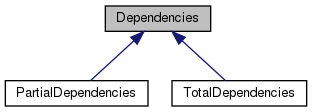
\includegraphics[width=306pt]{class_dependencies__inherit__graph}
\end{center}
\end{figure}
\subsection*{Public Member Functions}
\begin{DoxyCompactItemize}
\item 
\hyperlink{class_dependencies_afb4e8de48db17417cb0b3e5b57a17af4}{Dependencies} ()
\item 
virtual \hyperlink{class_dependencies_aeaa0706664765dd19c545f9683bf1aea}{$\sim$\+Dependencies} ()=0
\end{DoxyCompactItemize}


\subsection{Detailed Description}
Base class for dependencies. 

\subsection{Constructor \& Destructor Documentation}
\mbox{\Hypertarget{class_dependencies_afb4e8de48db17417cb0b3e5b57a17af4}\label{class_dependencies_afb4e8de48db17417cb0b3e5b57a17af4}} 
\index{Dependencies@{Dependencies}!Dependencies@{Dependencies}}
\index{Dependencies@{Dependencies}!Dependencies@{Dependencies}}
\subsubsection{\texorpdfstring{Dependencies()}{Dependencies()}}
{\footnotesize\ttfamily Dependencies\+::\+Dependencies (\begin{DoxyParamCaption}{ }\end{DoxyParamCaption})}

\mbox{\Hypertarget{class_dependencies_aeaa0706664765dd19c545f9683bf1aea}\label{class_dependencies_aeaa0706664765dd19c545f9683bf1aea}} 
\index{Dependencies@{Dependencies}!````~Dependencies@{$\sim$\+Dependencies}}
\index{````~Dependencies@{$\sim$\+Dependencies}!Dependencies@{Dependencies}}
\subsubsection{\texorpdfstring{$\sim$\+Dependencies()}{~Dependencies()}}
{\footnotesize\ttfamily Dependencies\+::$\sim$\+Dependencies (\begin{DoxyParamCaption}{ }\end{DoxyParamCaption})\hspace{0.3cm}{\ttfamily [pure virtual]}}



The documentation for this class was generated from the following files\+:\begin{DoxyCompactItemize}
\item 
src/\+Dependencies/\hyperlink{_dependencies_8h}{Dependencies.\+h}\item 
src/\+Dependencies/\hyperlink{_dependencies_8cc}{Dependencies.\+cc}\end{DoxyCompactItemize}

\hypertarget{class_dep_req}{}\section{Dep\+Req Class Reference}
\label{class_dep_req}\index{Dep\+Req@{Dep\+Req}}


Class generated from {\ttfamily Messages/dep\+Req.\+msg\+:32} by nedtool.  




{\ttfamily \#include $<$dep\+Req\+\_\+m.\+h$>$}



Inheritance diagram for Dep\+Req\+:
\nopagebreak
\begin{figure}[H]
\begin{center}
\leavevmode
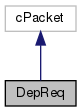
\includegraphics[width=133pt]{class_dep_req__inherit__graph}
\end{center}
\end{figure}


Collaboration diagram for Dep\+Req\+:
\nopagebreak
\begin{figure}[H]
\begin{center}
\leavevmode
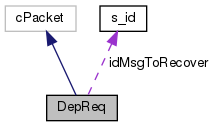
\includegraphics[width=233pt]{class_dep_req__coll__graph}
\end{center}
\end{figure}
\subsection*{Public Member Functions}
\begin{DoxyCompactItemize}
\item 
\hyperlink{class_dep_req_a133b51d43699e8ebecccf069935d93c4}{Dep\+Req} (const char $\ast$name=nullptr, short kind=0)
\item 
\hyperlink{class_dep_req_adf6800c87693c1de5b88d89c577186b8}{Dep\+Req} (const \hyperlink{class_dep_req}{Dep\+Req} \&other)
\item 
virtual \hyperlink{class_dep_req_a6f770d0327bf43dcef5f6a58f5a32183}{$\sim$\+Dep\+Req} ()
\item 
\hyperlink{class_dep_req}{Dep\+Req} \& \hyperlink{class_dep_req_a343eae743e4ca183897f0af8410d5ba3}{operator=} (const \hyperlink{class_dep_req}{Dep\+Req} \&other)
\item 
virtual \hyperlink{class_dep_req}{Dep\+Req} $\ast$ \hyperlink{class_dep_req_a430632dbd4f70a3a1183f226f0484bf3}{dup} () const override
\item 
virtual void \hyperlink{class_dep_req_a94c2def7b925be45621e20fd31e28e77}{parsim\+Pack} (omnetpp\+::c\+Comm\+Buffer $\ast$b) const override
\item 
virtual void \hyperlink{class_dep_req_a4fa8adb572938bc44f0a04463ea2df8d}{parsim\+Unpack} (omnetpp\+::c\+Comm\+Buffer $\ast$b) override
\item 
virtual \hyperlink{dep_req__m_8h_a2bbb71ed0e9660ec02d81471eafd9c29}{id\+Msg\+Dep\+Req} \& \hyperlink{class_dep_req_abbf56cc3e6a0be7ff696f9216f51f968}{get\+Id\+Msg\+To\+Recover} ()
\item 
virtual const \hyperlink{dep_req__m_8h_a2bbb71ed0e9660ec02d81471eafd9c29}{id\+Msg\+Dep\+Req} \& \hyperlink{class_dep_req_ab173923214b88b6c4b2f1d1cee8313d0}{get\+Id\+Msg\+To\+Recover} () const
\item 
virtual void \hyperlink{class_dep_req_a488a57f56c5fc87aae853a2b3e469fd0}{set\+Id\+Msg\+To\+Recover} (const \hyperlink{dep_req__m_8h_a2bbb71ed0e9660ec02d81471eafd9c29}{id\+Msg\+Dep\+Req} \&\hyperlink{class_dep_req_a8547e169d4670212c0b612924dda94cc}{id\+Msg\+To\+Recover})
\item 
virtual unsigned int \hyperlink{class_dep_req_a68f528e65d1529da94226f8a83483d6c}{get\+Id\+Requester} () const
\item 
virtual void \hyperlink{class_dep_req_a27f6e58ad8dcf4902de1042322a3e6e7}{set\+Id\+Requester} (unsigned int \hyperlink{class_dep_req_a26936e95ef3fae4753d2442318646c6b}{id\+Requester})
\item 
virtual \hyperlink{dep_req__m_8h_ae16a4057335e3a89fda3f6019868733b}{dep\+Req\+Time} \& \hyperlink{class_dep_req_a42fa35b3ced2cd9a4afd0ddeade48c19}{get\+Delay} ()
\item 
virtual const \hyperlink{dep_req__m_8h_ae16a4057335e3a89fda3f6019868733b}{dep\+Req\+Time} \& \hyperlink{class_dep_req_a3f686e18997f1383d0670a271d45a37b}{get\+Delay} () const
\item 
virtual void \hyperlink{class_dep_req_a90ae52243ec735ebf15bdf3e8467b393}{set\+Delay} (const \hyperlink{dep_req__m_8h_ae16a4057335e3a89fda3f6019868733b}{dep\+Req\+Time} \&\hyperlink{class_dep_req_a5df5ddeac692e25c089b458faf51e0c9}{delay})
\end{DoxyCompactItemize}
\subsection*{Protected Member Functions}
\begin{DoxyCompactItemize}
\item 
bool \hyperlink{class_dep_req_a0426b6cf870f2751d0933d7a9d56134c}{operator==} (const \hyperlink{class_dep_req}{Dep\+Req} \&)
\end{DoxyCompactItemize}
\subsection*{Protected Attributes}
\begin{DoxyCompactItemize}
\item 
\hyperlink{dep_req__m_8h_a2bbb71ed0e9660ec02d81471eafd9c29}{id\+Msg\+Dep\+Req} \hyperlink{class_dep_req_a8547e169d4670212c0b612924dda94cc}{id\+Msg\+To\+Recover}
\item 
unsigned int \hyperlink{class_dep_req_a26936e95ef3fae4753d2442318646c6b}{id\+Requester}
\item 
\hyperlink{dep_req__m_8h_ae16a4057335e3a89fda3f6019868733b}{dep\+Req\+Time} \hyperlink{class_dep_req_a5df5ddeac692e25c089b458faf51e0c9}{delay}
\end{DoxyCompactItemize}
\subsection*{Private Member Functions}
\begin{DoxyCompactItemize}
\item 
void \hyperlink{class_dep_req_a3ec88f2216d73f6b499ae6653a60437b}{copy} (const \hyperlink{class_dep_req}{Dep\+Req} \&other)
\end{DoxyCompactItemize}


\subsection{Detailed Description}
Class generated from {\ttfamily Messages/dep\+Req.\+msg\+:32} by nedtool. 


\begin{DoxyPre}
packet \hyperlink{class_dep_req}{DepReq}
\{
    idMsgDepReq idMsgToRecover;
    unsigned int idRequester; // debug
    depReqTime delay; // ms 
\}
\end{DoxyPre}
 

\subsection{Constructor \& Destructor Documentation}
\mbox{\Hypertarget{class_dep_req_a133b51d43699e8ebecccf069935d93c4}\label{class_dep_req_a133b51d43699e8ebecccf069935d93c4}} 
\index{Dep\+Req@{Dep\+Req}!Dep\+Req@{Dep\+Req}}
\index{Dep\+Req@{Dep\+Req}!Dep\+Req@{Dep\+Req}}
\subsubsection{\texorpdfstring{Dep\+Req()}{DepReq()}\hspace{0.1cm}{\footnotesize\ttfamily [1/2]}}
{\footnotesize\ttfamily Dep\+Req\+::\+Dep\+Req (\begin{DoxyParamCaption}\item[{const char $\ast$}]{name = {\ttfamily nullptr},  }\item[{short}]{kind = {\ttfamily 0} }\end{DoxyParamCaption})}

\mbox{\Hypertarget{class_dep_req_adf6800c87693c1de5b88d89c577186b8}\label{class_dep_req_adf6800c87693c1de5b88d89c577186b8}} 
\index{Dep\+Req@{Dep\+Req}!Dep\+Req@{Dep\+Req}}
\index{Dep\+Req@{Dep\+Req}!Dep\+Req@{Dep\+Req}}
\subsubsection{\texorpdfstring{Dep\+Req()}{DepReq()}\hspace{0.1cm}{\footnotesize\ttfamily [2/2]}}
{\footnotesize\ttfamily Dep\+Req\+::\+Dep\+Req (\begin{DoxyParamCaption}\item[{const \hyperlink{class_dep_req}{Dep\+Req} \&}]{other }\end{DoxyParamCaption})}

\mbox{\Hypertarget{class_dep_req_a6f770d0327bf43dcef5f6a58f5a32183}\label{class_dep_req_a6f770d0327bf43dcef5f6a58f5a32183}} 
\index{Dep\+Req@{Dep\+Req}!````~Dep\+Req@{$\sim$\+Dep\+Req}}
\index{````~Dep\+Req@{$\sim$\+Dep\+Req}!Dep\+Req@{Dep\+Req}}
\subsubsection{\texorpdfstring{$\sim$\+Dep\+Req()}{~DepReq()}}
{\footnotesize\ttfamily Dep\+Req\+::$\sim$\+Dep\+Req (\begin{DoxyParamCaption}{ }\end{DoxyParamCaption})\hspace{0.3cm}{\ttfamily [virtual]}}



\subsection{Member Function Documentation}
\mbox{\Hypertarget{class_dep_req_a3ec88f2216d73f6b499ae6653a60437b}\label{class_dep_req_a3ec88f2216d73f6b499ae6653a60437b}} 
\index{Dep\+Req@{Dep\+Req}!copy@{copy}}
\index{copy@{copy}!Dep\+Req@{Dep\+Req}}
\subsubsection{\texorpdfstring{copy()}{copy()}}
{\footnotesize\ttfamily void Dep\+Req\+::copy (\begin{DoxyParamCaption}\item[{const \hyperlink{class_dep_req}{Dep\+Req} \&}]{other }\end{DoxyParamCaption})\hspace{0.3cm}{\ttfamily [private]}}

\mbox{\Hypertarget{class_dep_req_a430632dbd4f70a3a1183f226f0484bf3}\label{class_dep_req_a430632dbd4f70a3a1183f226f0484bf3}} 
\index{Dep\+Req@{Dep\+Req}!dup@{dup}}
\index{dup@{dup}!Dep\+Req@{Dep\+Req}}
\subsubsection{\texorpdfstring{dup()}{dup()}}
{\footnotesize\ttfamily virtual \hyperlink{class_dep_req}{Dep\+Req}$\ast$ Dep\+Req\+::dup (\begin{DoxyParamCaption}{ }\end{DoxyParamCaption}) const\hspace{0.3cm}{\ttfamily [inline]}, {\ttfamily [override]}, {\ttfamily [virtual]}}

\mbox{\Hypertarget{class_dep_req_a42fa35b3ced2cd9a4afd0ddeade48c19}\label{class_dep_req_a42fa35b3ced2cd9a4afd0ddeade48c19}} 
\index{Dep\+Req@{Dep\+Req}!get\+Delay@{get\+Delay}}
\index{get\+Delay@{get\+Delay}!Dep\+Req@{Dep\+Req}}
\subsubsection{\texorpdfstring{get\+Delay()}{getDelay()}\hspace{0.1cm}{\footnotesize\ttfamily [1/2]}}
{\footnotesize\ttfamily \hyperlink{dep_req__m_8h_ae16a4057335e3a89fda3f6019868733b}{dep\+Req\+Time} \& Dep\+Req\+::get\+Delay (\begin{DoxyParamCaption}{ }\end{DoxyParamCaption})\hspace{0.3cm}{\ttfamily [virtual]}}

\mbox{\Hypertarget{class_dep_req_a3f686e18997f1383d0670a271d45a37b}\label{class_dep_req_a3f686e18997f1383d0670a271d45a37b}} 
\index{Dep\+Req@{Dep\+Req}!get\+Delay@{get\+Delay}}
\index{get\+Delay@{get\+Delay}!Dep\+Req@{Dep\+Req}}
\subsubsection{\texorpdfstring{get\+Delay()}{getDelay()}\hspace{0.1cm}{\footnotesize\ttfamily [2/2]}}
{\footnotesize\ttfamily virtual const \hyperlink{dep_req__m_8h_ae16a4057335e3a89fda3f6019868733b}{dep\+Req\+Time}\& Dep\+Req\+::get\+Delay (\begin{DoxyParamCaption}{ }\end{DoxyParamCaption}) const\hspace{0.3cm}{\ttfamily [inline]}, {\ttfamily [virtual]}}

\mbox{\Hypertarget{class_dep_req_abbf56cc3e6a0be7ff696f9216f51f968}\label{class_dep_req_abbf56cc3e6a0be7ff696f9216f51f968}} 
\index{Dep\+Req@{Dep\+Req}!get\+Id\+Msg\+To\+Recover@{get\+Id\+Msg\+To\+Recover}}
\index{get\+Id\+Msg\+To\+Recover@{get\+Id\+Msg\+To\+Recover}!Dep\+Req@{Dep\+Req}}
\subsubsection{\texorpdfstring{get\+Id\+Msg\+To\+Recover()}{getIdMsgToRecover()}\hspace{0.1cm}{\footnotesize\ttfamily [1/2]}}
{\footnotesize\ttfamily \hyperlink{dep_req__m_8h_a2bbb71ed0e9660ec02d81471eafd9c29}{id\+Msg\+Dep\+Req} \& Dep\+Req\+::get\+Id\+Msg\+To\+Recover (\begin{DoxyParamCaption}{ }\end{DoxyParamCaption})\hspace{0.3cm}{\ttfamily [virtual]}}

\mbox{\Hypertarget{class_dep_req_ab173923214b88b6c4b2f1d1cee8313d0}\label{class_dep_req_ab173923214b88b6c4b2f1d1cee8313d0}} 
\index{Dep\+Req@{Dep\+Req}!get\+Id\+Msg\+To\+Recover@{get\+Id\+Msg\+To\+Recover}}
\index{get\+Id\+Msg\+To\+Recover@{get\+Id\+Msg\+To\+Recover}!Dep\+Req@{Dep\+Req}}
\subsubsection{\texorpdfstring{get\+Id\+Msg\+To\+Recover()}{getIdMsgToRecover()}\hspace{0.1cm}{\footnotesize\ttfamily [2/2]}}
{\footnotesize\ttfamily virtual const \hyperlink{dep_req__m_8h_a2bbb71ed0e9660ec02d81471eafd9c29}{id\+Msg\+Dep\+Req}\& Dep\+Req\+::get\+Id\+Msg\+To\+Recover (\begin{DoxyParamCaption}{ }\end{DoxyParamCaption}) const\hspace{0.3cm}{\ttfamily [inline]}, {\ttfamily [virtual]}}

\mbox{\Hypertarget{class_dep_req_a68f528e65d1529da94226f8a83483d6c}\label{class_dep_req_a68f528e65d1529da94226f8a83483d6c}} 
\index{Dep\+Req@{Dep\+Req}!get\+Id\+Requester@{get\+Id\+Requester}}
\index{get\+Id\+Requester@{get\+Id\+Requester}!Dep\+Req@{Dep\+Req}}
\subsubsection{\texorpdfstring{get\+Id\+Requester()}{getIdRequester()}}
{\footnotesize\ttfamily unsigned int Dep\+Req\+::get\+Id\+Requester (\begin{DoxyParamCaption}{ }\end{DoxyParamCaption}) const\hspace{0.3cm}{\ttfamily [virtual]}}

\mbox{\Hypertarget{class_dep_req_a343eae743e4ca183897f0af8410d5ba3}\label{class_dep_req_a343eae743e4ca183897f0af8410d5ba3}} 
\index{Dep\+Req@{Dep\+Req}!operator=@{operator=}}
\index{operator=@{operator=}!Dep\+Req@{Dep\+Req}}
\subsubsection{\texorpdfstring{operator=()}{operator=()}}
{\footnotesize\ttfamily \hyperlink{class_dep_req}{Dep\+Req} \& Dep\+Req\+::operator= (\begin{DoxyParamCaption}\item[{const \hyperlink{class_dep_req}{Dep\+Req} \&}]{other }\end{DoxyParamCaption})}

\mbox{\Hypertarget{class_dep_req_a0426b6cf870f2751d0933d7a9d56134c}\label{class_dep_req_a0426b6cf870f2751d0933d7a9d56134c}} 
\index{Dep\+Req@{Dep\+Req}!operator==@{operator==}}
\index{operator==@{operator==}!Dep\+Req@{Dep\+Req}}
\subsubsection{\texorpdfstring{operator==()}{operator==()}}
{\footnotesize\ttfamily bool Dep\+Req\+::operator== (\begin{DoxyParamCaption}\item[{const \hyperlink{class_dep_req}{Dep\+Req} \&}]{ }\end{DoxyParamCaption})\hspace{0.3cm}{\ttfamily [protected]}}

\mbox{\Hypertarget{class_dep_req_a94c2def7b925be45621e20fd31e28e77}\label{class_dep_req_a94c2def7b925be45621e20fd31e28e77}} 
\index{Dep\+Req@{Dep\+Req}!parsim\+Pack@{parsim\+Pack}}
\index{parsim\+Pack@{parsim\+Pack}!Dep\+Req@{Dep\+Req}}
\subsubsection{\texorpdfstring{parsim\+Pack()}{parsimPack()}}
{\footnotesize\ttfamily void Dep\+Req\+::parsim\+Pack (\begin{DoxyParamCaption}\item[{omnetpp\+::c\+Comm\+Buffer $\ast$}]{b }\end{DoxyParamCaption}) const\hspace{0.3cm}{\ttfamily [override]}, {\ttfamily [virtual]}}

\mbox{\Hypertarget{class_dep_req_a4fa8adb572938bc44f0a04463ea2df8d}\label{class_dep_req_a4fa8adb572938bc44f0a04463ea2df8d}} 
\index{Dep\+Req@{Dep\+Req}!parsim\+Unpack@{parsim\+Unpack}}
\index{parsim\+Unpack@{parsim\+Unpack}!Dep\+Req@{Dep\+Req}}
\subsubsection{\texorpdfstring{parsim\+Unpack()}{parsimUnpack()}}
{\footnotesize\ttfamily void Dep\+Req\+::parsim\+Unpack (\begin{DoxyParamCaption}\item[{omnetpp\+::c\+Comm\+Buffer $\ast$}]{b }\end{DoxyParamCaption})\hspace{0.3cm}{\ttfamily [override]}, {\ttfamily [virtual]}}

\mbox{\Hypertarget{class_dep_req_a90ae52243ec735ebf15bdf3e8467b393}\label{class_dep_req_a90ae52243ec735ebf15bdf3e8467b393}} 
\index{Dep\+Req@{Dep\+Req}!set\+Delay@{set\+Delay}}
\index{set\+Delay@{set\+Delay}!Dep\+Req@{Dep\+Req}}
\subsubsection{\texorpdfstring{set\+Delay()}{setDelay()}}
{\footnotesize\ttfamily void Dep\+Req\+::set\+Delay (\begin{DoxyParamCaption}\item[{const \hyperlink{dep_req__m_8h_ae16a4057335e3a89fda3f6019868733b}{dep\+Req\+Time} \&}]{delay }\end{DoxyParamCaption})\hspace{0.3cm}{\ttfamily [virtual]}}

\mbox{\Hypertarget{class_dep_req_a488a57f56c5fc87aae853a2b3e469fd0}\label{class_dep_req_a488a57f56c5fc87aae853a2b3e469fd0}} 
\index{Dep\+Req@{Dep\+Req}!set\+Id\+Msg\+To\+Recover@{set\+Id\+Msg\+To\+Recover}}
\index{set\+Id\+Msg\+To\+Recover@{set\+Id\+Msg\+To\+Recover}!Dep\+Req@{Dep\+Req}}
\subsubsection{\texorpdfstring{set\+Id\+Msg\+To\+Recover()}{setIdMsgToRecover()}}
{\footnotesize\ttfamily void Dep\+Req\+::set\+Id\+Msg\+To\+Recover (\begin{DoxyParamCaption}\item[{const \hyperlink{dep_req__m_8h_a2bbb71ed0e9660ec02d81471eafd9c29}{id\+Msg\+Dep\+Req} \&}]{id\+Msg\+To\+Recover }\end{DoxyParamCaption})\hspace{0.3cm}{\ttfamily [virtual]}}

\mbox{\Hypertarget{class_dep_req_a27f6e58ad8dcf4902de1042322a3e6e7}\label{class_dep_req_a27f6e58ad8dcf4902de1042322a3e6e7}} 
\index{Dep\+Req@{Dep\+Req}!set\+Id\+Requester@{set\+Id\+Requester}}
\index{set\+Id\+Requester@{set\+Id\+Requester}!Dep\+Req@{Dep\+Req}}
\subsubsection{\texorpdfstring{set\+Id\+Requester()}{setIdRequester()}}
{\footnotesize\ttfamily void Dep\+Req\+::set\+Id\+Requester (\begin{DoxyParamCaption}\item[{unsigned int}]{id\+Requester }\end{DoxyParamCaption})\hspace{0.3cm}{\ttfamily [virtual]}}



\subsection{Member Data Documentation}
\mbox{\Hypertarget{class_dep_req_a5df5ddeac692e25c089b458faf51e0c9}\label{class_dep_req_a5df5ddeac692e25c089b458faf51e0c9}} 
\index{Dep\+Req@{Dep\+Req}!delay@{delay}}
\index{delay@{delay}!Dep\+Req@{Dep\+Req}}
\subsubsection{\texorpdfstring{delay}{delay}}
{\footnotesize\ttfamily \hyperlink{dep_req__m_8h_ae16a4057335e3a89fda3f6019868733b}{dep\+Req\+Time} Dep\+Req\+::delay\hspace{0.3cm}{\ttfamily [protected]}}

\mbox{\Hypertarget{class_dep_req_a8547e169d4670212c0b612924dda94cc}\label{class_dep_req_a8547e169d4670212c0b612924dda94cc}} 
\index{Dep\+Req@{Dep\+Req}!id\+Msg\+To\+Recover@{id\+Msg\+To\+Recover}}
\index{id\+Msg\+To\+Recover@{id\+Msg\+To\+Recover}!Dep\+Req@{Dep\+Req}}
\subsubsection{\texorpdfstring{id\+Msg\+To\+Recover}{idMsgToRecover}}
{\footnotesize\ttfamily \hyperlink{dep_req__m_8h_a2bbb71ed0e9660ec02d81471eafd9c29}{id\+Msg\+Dep\+Req} Dep\+Req\+::id\+Msg\+To\+Recover\hspace{0.3cm}{\ttfamily [protected]}}

\mbox{\Hypertarget{class_dep_req_a26936e95ef3fae4753d2442318646c6b}\label{class_dep_req_a26936e95ef3fae4753d2442318646c6b}} 
\index{Dep\+Req@{Dep\+Req}!id\+Requester@{id\+Requester}}
\index{id\+Requester@{id\+Requester}!Dep\+Req@{Dep\+Req}}
\subsubsection{\texorpdfstring{id\+Requester}{idRequester}}
{\footnotesize\ttfamily unsigned int Dep\+Req\+::id\+Requester\hspace{0.3cm}{\ttfamily [protected]}}



The documentation for this class was generated from the following files\+:\begin{DoxyCompactItemize}
\item 
/home/wilhelm/\+Documents/code\+Git\+Hub/\+Error\+Detectors/src/\+Messages/\hyperlink{dep_req__m_8h}{dep\+Req\+\_\+m.\+h}\item 
/home/wilhelm/\+Documents/code\+Git\+Hub/\+Error\+Detectors/src/\+Messages/\hyperlink{dep_req__m_8cc}{dep\+Req\+\_\+m.\+cc}\end{DoxyCompactItemize}

\hypertarget{class_dep_req_descriptor}{}\section{Dep\+Req\+Descriptor Class Reference}
\label{class_dep_req_descriptor}\index{Dep\+Req\+Descriptor@{Dep\+Req\+Descriptor}}


Inheritance diagram for Dep\+Req\+Descriptor\+:\nopagebreak
\begin{figure}[H]
\begin{center}
\leavevmode
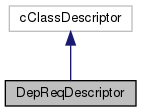
\includegraphics[width=178pt]{class_dep_req_descriptor__inherit__graph}
\end{center}
\end{figure}


Collaboration diagram for Dep\+Req\+Descriptor\+:\nopagebreak
\begin{figure}[H]
\begin{center}
\leavevmode
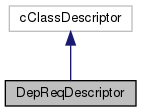
\includegraphics[width=178pt]{class_dep_req_descriptor__coll__graph}
\end{center}
\end{figure}
\subsection*{Public Member Functions}
\begin{DoxyCompactItemize}
\item 
\hyperlink{class_dep_req_descriptor_acc9a0e0eef48f3a21fc8ac17d63bf10a}{Dep\+Req\+Descriptor} ()
\item 
virtual \hyperlink{class_dep_req_descriptor_a68e3426897aa8baff48b1acae276c967}{$\sim$\+Dep\+Req\+Descriptor} ()
\item 
virtual bool \hyperlink{class_dep_req_descriptor_a1d6a05ff831c136608bac01b04cb8779}{does\+Support} (omnetpp\+::c\+Object $\ast$obj) const override
\item 
virtual const char $\ast$$\ast$ \hyperlink{class_dep_req_descriptor_a1b9e8ad7d683c9e2d1396e48fd7ec24f}{get\+Property\+Names} () const override
\item 
virtual const char $\ast$ \hyperlink{class_dep_req_descriptor_ae00fcc364ffe7494eaa0516f04c1e3f8}{get\+Property} (const char $\ast$propertyname) const override
\item 
virtual int \hyperlink{class_dep_req_descriptor_a7ca06e0d74b9a2eb7c335a935a52938f}{get\+Field\+Count} () const override
\item 
virtual const char $\ast$ \hyperlink{class_dep_req_descriptor_a8ef6ae7af9cb96791e005fd5e0c1e255}{get\+Field\+Name} (int field) const override
\item 
virtual int \hyperlink{class_dep_req_descriptor_a9c2af40c798a0d7bbb671f175734836c}{find\+Field} (const char $\ast$field\+Name) const override
\item 
virtual unsigned int \hyperlink{class_dep_req_descriptor_a67f19e0852007122a7ed1a3f773069ac}{get\+Field\+Type\+Flags} (int field) const override
\item 
virtual const char $\ast$ \hyperlink{class_dep_req_descriptor_abccd49184b08f6cbf98825c5cef37252}{get\+Field\+Type\+String} (int field) const override
\item 
virtual const char $\ast$$\ast$ \hyperlink{class_dep_req_descriptor_aedf5f2e33ed13cfb2d4584664dba743f}{get\+Field\+Property\+Names} (int field) const override
\item 
virtual const char $\ast$ \hyperlink{class_dep_req_descriptor_a86446083bf6eecb500c464288794e4a0}{get\+Field\+Property} (int field, const char $\ast$propertyname) const override
\item 
virtual int \hyperlink{class_dep_req_descriptor_a68402dadf251334b924fd9505c388bad}{get\+Field\+Array\+Size} (void $\ast$object, int field) const override
\item 
virtual const char $\ast$ \hyperlink{class_dep_req_descriptor_a734079401bce70ebe9dd48ebf997c8f1}{get\+Field\+Dynamic\+Type\+String} (void $\ast$object, int field, int i) const override
\item 
virtual std\+::string \hyperlink{class_dep_req_descriptor_a40708b1630241458821cbfce1e4dd79e}{get\+Field\+Value\+As\+String} (void $\ast$object, int field, int i) const override
\item 
virtual bool \hyperlink{class_dep_req_descriptor_af11c27d9903fc2d076855c9e1feda41b}{set\+Field\+Value\+As\+String} (void $\ast$object, int field, int i, const char $\ast$value) const override
\item 
virtual const char $\ast$ \hyperlink{class_dep_req_descriptor_acba71c972a19a687da42bb2c07baca42}{get\+Field\+Struct\+Name} (int field) const override
\item 
virtual void $\ast$ \hyperlink{class_dep_req_descriptor_a9022933bea91f71f62d6dc8befb94310}{get\+Field\+Struct\+Value\+Pointer} (void $\ast$object, int field, int i) const override
\end{DoxyCompactItemize}
\subsection*{Private Attributes}
\begin{DoxyCompactItemize}
\item 
const char $\ast$$\ast$ \hyperlink{class_dep_req_descriptor_a0d724047f7da4672219cb81300cfbdd4}{propertynames}
\end{DoxyCompactItemize}


\subsection{Constructor \& Destructor Documentation}
\mbox{\Hypertarget{class_dep_req_descriptor_acc9a0e0eef48f3a21fc8ac17d63bf10a}\label{class_dep_req_descriptor_acc9a0e0eef48f3a21fc8ac17d63bf10a}} 
\index{Dep\+Req\+Descriptor@{Dep\+Req\+Descriptor}!Dep\+Req\+Descriptor@{Dep\+Req\+Descriptor}}
\index{Dep\+Req\+Descriptor@{Dep\+Req\+Descriptor}!Dep\+Req\+Descriptor@{Dep\+Req\+Descriptor}}
\subsubsection{\texorpdfstring{Dep\+Req\+Descriptor()}{DepReqDescriptor()}}
{\footnotesize\ttfamily Dep\+Req\+Descriptor\+::\+Dep\+Req\+Descriptor (\begin{DoxyParamCaption}{ }\end{DoxyParamCaption})}

\mbox{\Hypertarget{class_dep_req_descriptor_a68e3426897aa8baff48b1acae276c967}\label{class_dep_req_descriptor_a68e3426897aa8baff48b1acae276c967}} 
\index{Dep\+Req\+Descriptor@{Dep\+Req\+Descriptor}!````~Dep\+Req\+Descriptor@{$\sim$\+Dep\+Req\+Descriptor}}
\index{````~Dep\+Req\+Descriptor@{$\sim$\+Dep\+Req\+Descriptor}!Dep\+Req\+Descriptor@{Dep\+Req\+Descriptor}}
\subsubsection{\texorpdfstring{$\sim$\+Dep\+Req\+Descriptor()}{~DepReqDescriptor()}}
{\footnotesize\ttfamily Dep\+Req\+Descriptor\+::$\sim$\+Dep\+Req\+Descriptor (\begin{DoxyParamCaption}{ }\end{DoxyParamCaption})\hspace{0.3cm}{\ttfamily [virtual]}}



\subsection{Member Function Documentation}
\mbox{\Hypertarget{class_dep_req_descriptor_a1d6a05ff831c136608bac01b04cb8779}\label{class_dep_req_descriptor_a1d6a05ff831c136608bac01b04cb8779}} 
\index{Dep\+Req\+Descriptor@{Dep\+Req\+Descriptor}!does\+Support@{does\+Support}}
\index{does\+Support@{does\+Support}!Dep\+Req\+Descriptor@{Dep\+Req\+Descriptor}}
\subsubsection{\texorpdfstring{does\+Support()}{doesSupport()}}
{\footnotesize\ttfamily bool Dep\+Req\+Descriptor\+::does\+Support (\begin{DoxyParamCaption}\item[{omnetpp\+::c\+Object $\ast$}]{obj }\end{DoxyParamCaption}) const\hspace{0.3cm}{\ttfamily [override]}, {\ttfamily [virtual]}}

\mbox{\Hypertarget{class_dep_req_descriptor_a9c2af40c798a0d7bbb671f175734836c}\label{class_dep_req_descriptor_a9c2af40c798a0d7bbb671f175734836c}} 
\index{Dep\+Req\+Descriptor@{Dep\+Req\+Descriptor}!find\+Field@{find\+Field}}
\index{find\+Field@{find\+Field}!Dep\+Req\+Descriptor@{Dep\+Req\+Descriptor}}
\subsubsection{\texorpdfstring{find\+Field()}{findField()}}
{\footnotesize\ttfamily int Dep\+Req\+Descriptor\+::find\+Field (\begin{DoxyParamCaption}\item[{const char $\ast$}]{field\+Name }\end{DoxyParamCaption}) const\hspace{0.3cm}{\ttfamily [override]}, {\ttfamily [virtual]}}

\mbox{\Hypertarget{class_dep_req_descriptor_a68402dadf251334b924fd9505c388bad}\label{class_dep_req_descriptor_a68402dadf251334b924fd9505c388bad}} 
\index{Dep\+Req\+Descriptor@{Dep\+Req\+Descriptor}!get\+Field\+Array\+Size@{get\+Field\+Array\+Size}}
\index{get\+Field\+Array\+Size@{get\+Field\+Array\+Size}!Dep\+Req\+Descriptor@{Dep\+Req\+Descriptor}}
\subsubsection{\texorpdfstring{get\+Field\+Array\+Size()}{getFieldArraySize()}}
{\footnotesize\ttfamily int Dep\+Req\+Descriptor\+::get\+Field\+Array\+Size (\begin{DoxyParamCaption}\item[{void $\ast$}]{object,  }\item[{int}]{field }\end{DoxyParamCaption}) const\hspace{0.3cm}{\ttfamily [override]}, {\ttfamily [virtual]}}

\mbox{\Hypertarget{class_dep_req_descriptor_a7ca06e0d74b9a2eb7c335a935a52938f}\label{class_dep_req_descriptor_a7ca06e0d74b9a2eb7c335a935a52938f}} 
\index{Dep\+Req\+Descriptor@{Dep\+Req\+Descriptor}!get\+Field\+Count@{get\+Field\+Count}}
\index{get\+Field\+Count@{get\+Field\+Count}!Dep\+Req\+Descriptor@{Dep\+Req\+Descriptor}}
\subsubsection{\texorpdfstring{get\+Field\+Count()}{getFieldCount()}}
{\footnotesize\ttfamily int Dep\+Req\+Descriptor\+::get\+Field\+Count (\begin{DoxyParamCaption}{ }\end{DoxyParamCaption}) const\hspace{0.3cm}{\ttfamily [override]}, {\ttfamily [virtual]}}

\mbox{\Hypertarget{class_dep_req_descriptor_a734079401bce70ebe9dd48ebf997c8f1}\label{class_dep_req_descriptor_a734079401bce70ebe9dd48ebf997c8f1}} 
\index{Dep\+Req\+Descriptor@{Dep\+Req\+Descriptor}!get\+Field\+Dynamic\+Type\+String@{get\+Field\+Dynamic\+Type\+String}}
\index{get\+Field\+Dynamic\+Type\+String@{get\+Field\+Dynamic\+Type\+String}!Dep\+Req\+Descriptor@{Dep\+Req\+Descriptor}}
\subsubsection{\texorpdfstring{get\+Field\+Dynamic\+Type\+String()}{getFieldDynamicTypeString()}}
{\footnotesize\ttfamily const char $\ast$ Dep\+Req\+Descriptor\+::get\+Field\+Dynamic\+Type\+String (\begin{DoxyParamCaption}\item[{void $\ast$}]{object,  }\item[{int}]{field,  }\item[{int}]{i }\end{DoxyParamCaption}) const\hspace{0.3cm}{\ttfamily [override]}, {\ttfamily [virtual]}}

\mbox{\Hypertarget{class_dep_req_descriptor_a8ef6ae7af9cb96791e005fd5e0c1e255}\label{class_dep_req_descriptor_a8ef6ae7af9cb96791e005fd5e0c1e255}} 
\index{Dep\+Req\+Descriptor@{Dep\+Req\+Descriptor}!get\+Field\+Name@{get\+Field\+Name}}
\index{get\+Field\+Name@{get\+Field\+Name}!Dep\+Req\+Descriptor@{Dep\+Req\+Descriptor}}
\subsubsection{\texorpdfstring{get\+Field\+Name()}{getFieldName()}}
{\footnotesize\ttfamily const char $\ast$ Dep\+Req\+Descriptor\+::get\+Field\+Name (\begin{DoxyParamCaption}\item[{int}]{field }\end{DoxyParamCaption}) const\hspace{0.3cm}{\ttfamily [override]}, {\ttfamily [virtual]}}

\mbox{\Hypertarget{class_dep_req_descriptor_a86446083bf6eecb500c464288794e4a0}\label{class_dep_req_descriptor_a86446083bf6eecb500c464288794e4a0}} 
\index{Dep\+Req\+Descriptor@{Dep\+Req\+Descriptor}!get\+Field\+Property@{get\+Field\+Property}}
\index{get\+Field\+Property@{get\+Field\+Property}!Dep\+Req\+Descriptor@{Dep\+Req\+Descriptor}}
\subsubsection{\texorpdfstring{get\+Field\+Property()}{getFieldProperty()}}
{\footnotesize\ttfamily const char $\ast$ Dep\+Req\+Descriptor\+::get\+Field\+Property (\begin{DoxyParamCaption}\item[{int}]{field,  }\item[{const char $\ast$}]{propertyname }\end{DoxyParamCaption}) const\hspace{0.3cm}{\ttfamily [override]}, {\ttfamily [virtual]}}

\mbox{\Hypertarget{class_dep_req_descriptor_aedf5f2e33ed13cfb2d4584664dba743f}\label{class_dep_req_descriptor_aedf5f2e33ed13cfb2d4584664dba743f}} 
\index{Dep\+Req\+Descriptor@{Dep\+Req\+Descriptor}!get\+Field\+Property\+Names@{get\+Field\+Property\+Names}}
\index{get\+Field\+Property\+Names@{get\+Field\+Property\+Names}!Dep\+Req\+Descriptor@{Dep\+Req\+Descriptor}}
\subsubsection{\texorpdfstring{get\+Field\+Property\+Names()}{getFieldPropertyNames()}}
{\footnotesize\ttfamily const char $\ast$$\ast$ Dep\+Req\+Descriptor\+::get\+Field\+Property\+Names (\begin{DoxyParamCaption}\item[{int}]{field }\end{DoxyParamCaption}) const\hspace{0.3cm}{\ttfamily [override]}, {\ttfamily [virtual]}}

\mbox{\Hypertarget{class_dep_req_descriptor_acba71c972a19a687da42bb2c07baca42}\label{class_dep_req_descriptor_acba71c972a19a687da42bb2c07baca42}} 
\index{Dep\+Req\+Descriptor@{Dep\+Req\+Descriptor}!get\+Field\+Struct\+Name@{get\+Field\+Struct\+Name}}
\index{get\+Field\+Struct\+Name@{get\+Field\+Struct\+Name}!Dep\+Req\+Descriptor@{Dep\+Req\+Descriptor}}
\subsubsection{\texorpdfstring{get\+Field\+Struct\+Name()}{getFieldStructName()}}
{\footnotesize\ttfamily const char $\ast$ Dep\+Req\+Descriptor\+::get\+Field\+Struct\+Name (\begin{DoxyParamCaption}\item[{int}]{field }\end{DoxyParamCaption}) const\hspace{0.3cm}{\ttfamily [override]}, {\ttfamily [virtual]}}

\mbox{\Hypertarget{class_dep_req_descriptor_a9022933bea91f71f62d6dc8befb94310}\label{class_dep_req_descriptor_a9022933bea91f71f62d6dc8befb94310}} 
\index{Dep\+Req\+Descriptor@{Dep\+Req\+Descriptor}!get\+Field\+Struct\+Value\+Pointer@{get\+Field\+Struct\+Value\+Pointer}}
\index{get\+Field\+Struct\+Value\+Pointer@{get\+Field\+Struct\+Value\+Pointer}!Dep\+Req\+Descriptor@{Dep\+Req\+Descriptor}}
\subsubsection{\texorpdfstring{get\+Field\+Struct\+Value\+Pointer()}{getFieldStructValuePointer()}}
{\footnotesize\ttfamily void $\ast$ Dep\+Req\+Descriptor\+::get\+Field\+Struct\+Value\+Pointer (\begin{DoxyParamCaption}\item[{void $\ast$}]{object,  }\item[{int}]{field,  }\item[{int}]{i }\end{DoxyParamCaption}) const\hspace{0.3cm}{\ttfamily [override]}, {\ttfamily [virtual]}}

\mbox{\Hypertarget{class_dep_req_descriptor_a67f19e0852007122a7ed1a3f773069ac}\label{class_dep_req_descriptor_a67f19e0852007122a7ed1a3f773069ac}} 
\index{Dep\+Req\+Descriptor@{Dep\+Req\+Descriptor}!get\+Field\+Type\+Flags@{get\+Field\+Type\+Flags}}
\index{get\+Field\+Type\+Flags@{get\+Field\+Type\+Flags}!Dep\+Req\+Descriptor@{Dep\+Req\+Descriptor}}
\subsubsection{\texorpdfstring{get\+Field\+Type\+Flags()}{getFieldTypeFlags()}}
{\footnotesize\ttfamily unsigned int Dep\+Req\+Descriptor\+::get\+Field\+Type\+Flags (\begin{DoxyParamCaption}\item[{int}]{field }\end{DoxyParamCaption}) const\hspace{0.3cm}{\ttfamily [override]}, {\ttfamily [virtual]}}

\mbox{\Hypertarget{class_dep_req_descriptor_abccd49184b08f6cbf98825c5cef37252}\label{class_dep_req_descriptor_abccd49184b08f6cbf98825c5cef37252}} 
\index{Dep\+Req\+Descriptor@{Dep\+Req\+Descriptor}!get\+Field\+Type\+String@{get\+Field\+Type\+String}}
\index{get\+Field\+Type\+String@{get\+Field\+Type\+String}!Dep\+Req\+Descriptor@{Dep\+Req\+Descriptor}}
\subsubsection{\texorpdfstring{get\+Field\+Type\+String()}{getFieldTypeString()}}
{\footnotesize\ttfamily const char $\ast$ Dep\+Req\+Descriptor\+::get\+Field\+Type\+String (\begin{DoxyParamCaption}\item[{int}]{field }\end{DoxyParamCaption}) const\hspace{0.3cm}{\ttfamily [override]}, {\ttfamily [virtual]}}

\mbox{\Hypertarget{class_dep_req_descriptor_a40708b1630241458821cbfce1e4dd79e}\label{class_dep_req_descriptor_a40708b1630241458821cbfce1e4dd79e}} 
\index{Dep\+Req\+Descriptor@{Dep\+Req\+Descriptor}!get\+Field\+Value\+As\+String@{get\+Field\+Value\+As\+String}}
\index{get\+Field\+Value\+As\+String@{get\+Field\+Value\+As\+String}!Dep\+Req\+Descriptor@{Dep\+Req\+Descriptor}}
\subsubsection{\texorpdfstring{get\+Field\+Value\+As\+String()}{getFieldValueAsString()}}
{\footnotesize\ttfamily std\+::string Dep\+Req\+Descriptor\+::get\+Field\+Value\+As\+String (\begin{DoxyParamCaption}\item[{void $\ast$}]{object,  }\item[{int}]{field,  }\item[{int}]{i }\end{DoxyParamCaption}) const\hspace{0.3cm}{\ttfamily [override]}, {\ttfamily [virtual]}}

\mbox{\Hypertarget{class_dep_req_descriptor_ae00fcc364ffe7494eaa0516f04c1e3f8}\label{class_dep_req_descriptor_ae00fcc364ffe7494eaa0516f04c1e3f8}} 
\index{Dep\+Req\+Descriptor@{Dep\+Req\+Descriptor}!get\+Property@{get\+Property}}
\index{get\+Property@{get\+Property}!Dep\+Req\+Descriptor@{Dep\+Req\+Descriptor}}
\subsubsection{\texorpdfstring{get\+Property()}{getProperty()}}
{\footnotesize\ttfamily const char $\ast$ Dep\+Req\+Descriptor\+::get\+Property (\begin{DoxyParamCaption}\item[{const char $\ast$}]{propertyname }\end{DoxyParamCaption}) const\hspace{0.3cm}{\ttfamily [override]}, {\ttfamily [virtual]}}

\mbox{\Hypertarget{class_dep_req_descriptor_a1b9e8ad7d683c9e2d1396e48fd7ec24f}\label{class_dep_req_descriptor_a1b9e8ad7d683c9e2d1396e48fd7ec24f}} 
\index{Dep\+Req\+Descriptor@{Dep\+Req\+Descriptor}!get\+Property\+Names@{get\+Property\+Names}}
\index{get\+Property\+Names@{get\+Property\+Names}!Dep\+Req\+Descriptor@{Dep\+Req\+Descriptor}}
\subsubsection{\texorpdfstring{get\+Property\+Names()}{getPropertyNames()}}
{\footnotesize\ttfamily const char $\ast$$\ast$ Dep\+Req\+Descriptor\+::get\+Property\+Names (\begin{DoxyParamCaption}{ }\end{DoxyParamCaption}) const\hspace{0.3cm}{\ttfamily [override]}, {\ttfamily [virtual]}}

\mbox{\Hypertarget{class_dep_req_descriptor_af11c27d9903fc2d076855c9e1feda41b}\label{class_dep_req_descriptor_af11c27d9903fc2d076855c9e1feda41b}} 
\index{Dep\+Req\+Descriptor@{Dep\+Req\+Descriptor}!set\+Field\+Value\+As\+String@{set\+Field\+Value\+As\+String}}
\index{set\+Field\+Value\+As\+String@{set\+Field\+Value\+As\+String}!Dep\+Req\+Descriptor@{Dep\+Req\+Descriptor}}
\subsubsection{\texorpdfstring{set\+Field\+Value\+As\+String()}{setFieldValueAsString()}}
{\footnotesize\ttfamily bool Dep\+Req\+Descriptor\+::set\+Field\+Value\+As\+String (\begin{DoxyParamCaption}\item[{void $\ast$}]{object,  }\item[{int}]{field,  }\item[{int}]{i,  }\item[{const char $\ast$}]{value }\end{DoxyParamCaption}) const\hspace{0.3cm}{\ttfamily [override]}, {\ttfamily [virtual]}}



\subsection{Member Data Documentation}
\mbox{\Hypertarget{class_dep_req_descriptor_a0d724047f7da4672219cb81300cfbdd4}\label{class_dep_req_descriptor_a0d724047f7da4672219cb81300cfbdd4}} 
\index{Dep\+Req\+Descriptor@{Dep\+Req\+Descriptor}!propertynames@{propertynames}}
\index{propertynames@{propertynames}!Dep\+Req\+Descriptor@{Dep\+Req\+Descriptor}}
\subsubsection{\texorpdfstring{propertynames}{propertynames}}
{\footnotesize\ttfamily const char$\ast$$\ast$ Dep\+Req\+Descriptor\+::propertynames\hspace{0.3cm}{\ttfamily [mutable]}, {\ttfamily [private]}}



The documentation for this class was generated from the following file\+:\begin{DoxyCompactItemize}
\item 
src/\+Messages/\hyperlink{dep_req__m_8cc}{dep\+Req\+\_\+m.\+cc}\end{DoxyCompactItemize}

\hypertarget{classdep_req_time_descriptor}{}\section{dep\+Req\+Time\+Descriptor Class Reference}
\label{classdep_req_time_descriptor}\index{dep\+Req\+Time\+Descriptor@{dep\+Req\+Time\+Descriptor}}


Inheritance diagram for dep\+Req\+Time\+Descriptor\+:
\nopagebreak
\begin{figure}[H]
\begin{center}
\leavevmode
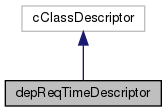
\includegraphics[width=197pt]{classdep_req_time_descriptor__inherit__graph}
\end{center}
\end{figure}


Collaboration diagram for dep\+Req\+Time\+Descriptor\+:
\nopagebreak
\begin{figure}[H]
\begin{center}
\leavevmode
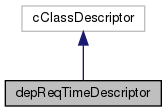
\includegraphics[width=197pt]{classdep_req_time_descriptor__coll__graph}
\end{center}
\end{figure}
\subsection*{Public Member Functions}
\begin{DoxyCompactItemize}
\item 
\hyperlink{classdep_req_time_descriptor_a3a2e6770051714ad9759ccbf1943dbff}{dep\+Req\+Time\+Descriptor} ()
\item 
virtual \hyperlink{classdep_req_time_descriptor_ab1e88d4e75d0da895acc20d8bbb28f45}{$\sim$dep\+Req\+Time\+Descriptor} ()
\item 
virtual bool \hyperlink{classdep_req_time_descriptor_a919fa187f7ad370fa29f389841b15310}{does\+Support} (omnetpp\+::c\+Object $\ast$obj) const override
\item 
virtual const char $\ast$$\ast$ \hyperlink{classdep_req_time_descriptor_a9f361ef5b255d6cf9846e52b67f5e837}{get\+Property\+Names} () const override
\item 
virtual const char $\ast$ \hyperlink{classdep_req_time_descriptor_a31c4397606ef6ed7e21621d51c4498fb}{get\+Property} (const char $\ast$propertyname) const override
\item 
virtual int \hyperlink{classdep_req_time_descriptor_a079564e7bacb79e8be6d3af9286ba54b}{get\+Field\+Count} () const override
\item 
virtual const char $\ast$ \hyperlink{classdep_req_time_descriptor_aa59fd9802c965acfb3876b88f26a2f0d}{get\+Field\+Name} (int field) const override
\item 
virtual int \hyperlink{classdep_req_time_descriptor_abdf669cde2ee94741db7eaa3bd4a61bf}{find\+Field} (const char $\ast$field\+Name) const override
\item 
virtual unsigned int \hyperlink{classdep_req_time_descriptor_ab1f3fdc98b07adfe47aecf2a122690ee}{get\+Field\+Type\+Flags} (int field) const override
\item 
virtual const char $\ast$ \hyperlink{classdep_req_time_descriptor_af28f6a1029b87177e101167d3fc89c3b}{get\+Field\+Type\+String} (int field) const override
\item 
virtual const char $\ast$$\ast$ \hyperlink{classdep_req_time_descriptor_aa20459216b1c8dfecebfed86c43aa6d2}{get\+Field\+Property\+Names} (int field) const override
\item 
virtual const char $\ast$ \hyperlink{classdep_req_time_descriptor_aee85faec811f0a52f2d112ea46689d73}{get\+Field\+Property} (int field, const char $\ast$propertyname) const override
\item 
virtual int \hyperlink{classdep_req_time_descriptor_a4d6a51a338076853385eb86d734319d4}{get\+Field\+Array\+Size} (void $\ast$object, int field) const override
\item 
virtual const char $\ast$ \hyperlink{classdep_req_time_descriptor_a8c3f7004d1d8f89cbb01bd7e827f1ad8}{get\+Field\+Dynamic\+Type\+String} (void $\ast$object, int field, int i) const override
\item 
virtual std\+::string \hyperlink{classdep_req_time_descriptor_a93ae2e8b0dece6757eabe758959988fd}{get\+Field\+Value\+As\+String} (void $\ast$object, int field, int i) const override
\item 
virtual bool \hyperlink{classdep_req_time_descriptor_a03a2b4c17daaad8eb395d571279dde51}{set\+Field\+Value\+As\+String} (void $\ast$object, int field, int i, const char $\ast$value) const override
\item 
virtual const char $\ast$ \hyperlink{classdep_req_time_descriptor_a5d68aab012514ac2d7f4649412b98ec0}{get\+Field\+Struct\+Name} (int field) const override
\item 
virtual void $\ast$ \hyperlink{classdep_req_time_descriptor_a886868d18593658df92a25dd43eedcaf}{get\+Field\+Struct\+Value\+Pointer} (void $\ast$object, int field, int i) const override
\end{DoxyCompactItemize}
\subsection*{Private Attributes}
\begin{DoxyCompactItemize}
\item 
const char $\ast$$\ast$ \hyperlink{classdep_req_time_descriptor_a8027018b5fe1aeb72652563cd2a9f505}{propertynames}
\end{DoxyCompactItemize}


\subsection{Constructor \& Destructor Documentation}
\mbox{\Hypertarget{classdep_req_time_descriptor_a3a2e6770051714ad9759ccbf1943dbff}\label{classdep_req_time_descriptor_a3a2e6770051714ad9759ccbf1943dbff}} 
\index{dep\+Req\+Time\+Descriptor@{dep\+Req\+Time\+Descriptor}!dep\+Req\+Time\+Descriptor@{dep\+Req\+Time\+Descriptor}}
\index{dep\+Req\+Time\+Descriptor@{dep\+Req\+Time\+Descriptor}!dep\+Req\+Time\+Descriptor@{dep\+Req\+Time\+Descriptor}}
\subsubsection{\texorpdfstring{dep\+Req\+Time\+Descriptor()}{depReqTimeDescriptor()}}
{\footnotesize\ttfamily dep\+Req\+Time\+Descriptor\+::dep\+Req\+Time\+Descriptor (\begin{DoxyParamCaption}{ }\end{DoxyParamCaption})}

\mbox{\Hypertarget{classdep_req_time_descriptor_ab1e88d4e75d0da895acc20d8bbb28f45}\label{classdep_req_time_descriptor_ab1e88d4e75d0da895acc20d8bbb28f45}} 
\index{dep\+Req\+Time\+Descriptor@{dep\+Req\+Time\+Descriptor}!````~dep\+Req\+Time\+Descriptor@{$\sim$dep\+Req\+Time\+Descriptor}}
\index{````~dep\+Req\+Time\+Descriptor@{$\sim$dep\+Req\+Time\+Descriptor}!dep\+Req\+Time\+Descriptor@{dep\+Req\+Time\+Descriptor}}
\subsubsection{\texorpdfstring{$\sim$dep\+Req\+Time\+Descriptor()}{~depReqTimeDescriptor()}}
{\footnotesize\ttfamily dep\+Req\+Time\+Descriptor\+::$\sim$dep\+Req\+Time\+Descriptor (\begin{DoxyParamCaption}{ }\end{DoxyParamCaption})\hspace{0.3cm}{\ttfamily [virtual]}}



\subsection{Member Function Documentation}
\mbox{\Hypertarget{classdep_req_time_descriptor_a919fa187f7ad370fa29f389841b15310}\label{classdep_req_time_descriptor_a919fa187f7ad370fa29f389841b15310}} 
\index{dep\+Req\+Time\+Descriptor@{dep\+Req\+Time\+Descriptor}!does\+Support@{does\+Support}}
\index{does\+Support@{does\+Support}!dep\+Req\+Time\+Descriptor@{dep\+Req\+Time\+Descriptor}}
\subsubsection{\texorpdfstring{does\+Support()}{doesSupport()}}
{\footnotesize\ttfamily bool dep\+Req\+Time\+Descriptor\+::does\+Support (\begin{DoxyParamCaption}\item[{omnetpp\+::c\+Object $\ast$}]{obj }\end{DoxyParamCaption}) const\hspace{0.3cm}{\ttfamily [override]}, {\ttfamily [virtual]}}

\mbox{\Hypertarget{classdep_req_time_descriptor_abdf669cde2ee94741db7eaa3bd4a61bf}\label{classdep_req_time_descriptor_abdf669cde2ee94741db7eaa3bd4a61bf}} 
\index{dep\+Req\+Time\+Descriptor@{dep\+Req\+Time\+Descriptor}!find\+Field@{find\+Field}}
\index{find\+Field@{find\+Field}!dep\+Req\+Time\+Descriptor@{dep\+Req\+Time\+Descriptor}}
\subsubsection{\texorpdfstring{find\+Field()}{findField()}}
{\footnotesize\ttfamily int dep\+Req\+Time\+Descriptor\+::find\+Field (\begin{DoxyParamCaption}\item[{const char $\ast$}]{field\+Name }\end{DoxyParamCaption}) const\hspace{0.3cm}{\ttfamily [override]}, {\ttfamily [virtual]}}

\mbox{\Hypertarget{classdep_req_time_descriptor_a4d6a51a338076853385eb86d734319d4}\label{classdep_req_time_descriptor_a4d6a51a338076853385eb86d734319d4}} 
\index{dep\+Req\+Time\+Descriptor@{dep\+Req\+Time\+Descriptor}!get\+Field\+Array\+Size@{get\+Field\+Array\+Size}}
\index{get\+Field\+Array\+Size@{get\+Field\+Array\+Size}!dep\+Req\+Time\+Descriptor@{dep\+Req\+Time\+Descriptor}}
\subsubsection{\texorpdfstring{get\+Field\+Array\+Size()}{getFieldArraySize()}}
{\footnotesize\ttfamily int dep\+Req\+Time\+Descriptor\+::get\+Field\+Array\+Size (\begin{DoxyParamCaption}\item[{void $\ast$}]{object,  }\item[{int}]{field }\end{DoxyParamCaption}) const\hspace{0.3cm}{\ttfamily [override]}, {\ttfamily [virtual]}}

\mbox{\Hypertarget{classdep_req_time_descriptor_a079564e7bacb79e8be6d3af9286ba54b}\label{classdep_req_time_descriptor_a079564e7bacb79e8be6d3af9286ba54b}} 
\index{dep\+Req\+Time\+Descriptor@{dep\+Req\+Time\+Descriptor}!get\+Field\+Count@{get\+Field\+Count}}
\index{get\+Field\+Count@{get\+Field\+Count}!dep\+Req\+Time\+Descriptor@{dep\+Req\+Time\+Descriptor}}
\subsubsection{\texorpdfstring{get\+Field\+Count()}{getFieldCount()}}
{\footnotesize\ttfamily int dep\+Req\+Time\+Descriptor\+::get\+Field\+Count (\begin{DoxyParamCaption}{ }\end{DoxyParamCaption}) const\hspace{0.3cm}{\ttfamily [override]}, {\ttfamily [virtual]}}

\mbox{\Hypertarget{classdep_req_time_descriptor_a8c3f7004d1d8f89cbb01bd7e827f1ad8}\label{classdep_req_time_descriptor_a8c3f7004d1d8f89cbb01bd7e827f1ad8}} 
\index{dep\+Req\+Time\+Descriptor@{dep\+Req\+Time\+Descriptor}!get\+Field\+Dynamic\+Type\+String@{get\+Field\+Dynamic\+Type\+String}}
\index{get\+Field\+Dynamic\+Type\+String@{get\+Field\+Dynamic\+Type\+String}!dep\+Req\+Time\+Descriptor@{dep\+Req\+Time\+Descriptor}}
\subsubsection{\texorpdfstring{get\+Field\+Dynamic\+Type\+String()}{getFieldDynamicTypeString()}}
{\footnotesize\ttfamily const char $\ast$ dep\+Req\+Time\+Descriptor\+::get\+Field\+Dynamic\+Type\+String (\begin{DoxyParamCaption}\item[{void $\ast$}]{object,  }\item[{int}]{field,  }\item[{int}]{i }\end{DoxyParamCaption}) const\hspace{0.3cm}{\ttfamily [override]}, {\ttfamily [virtual]}}

\mbox{\Hypertarget{classdep_req_time_descriptor_aa59fd9802c965acfb3876b88f26a2f0d}\label{classdep_req_time_descriptor_aa59fd9802c965acfb3876b88f26a2f0d}} 
\index{dep\+Req\+Time\+Descriptor@{dep\+Req\+Time\+Descriptor}!get\+Field\+Name@{get\+Field\+Name}}
\index{get\+Field\+Name@{get\+Field\+Name}!dep\+Req\+Time\+Descriptor@{dep\+Req\+Time\+Descriptor}}
\subsubsection{\texorpdfstring{get\+Field\+Name()}{getFieldName()}}
{\footnotesize\ttfamily const char $\ast$ dep\+Req\+Time\+Descriptor\+::get\+Field\+Name (\begin{DoxyParamCaption}\item[{int}]{field }\end{DoxyParamCaption}) const\hspace{0.3cm}{\ttfamily [override]}, {\ttfamily [virtual]}}

\mbox{\Hypertarget{classdep_req_time_descriptor_aee85faec811f0a52f2d112ea46689d73}\label{classdep_req_time_descriptor_aee85faec811f0a52f2d112ea46689d73}} 
\index{dep\+Req\+Time\+Descriptor@{dep\+Req\+Time\+Descriptor}!get\+Field\+Property@{get\+Field\+Property}}
\index{get\+Field\+Property@{get\+Field\+Property}!dep\+Req\+Time\+Descriptor@{dep\+Req\+Time\+Descriptor}}
\subsubsection{\texorpdfstring{get\+Field\+Property()}{getFieldProperty()}}
{\footnotesize\ttfamily const char $\ast$ dep\+Req\+Time\+Descriptor\+::get\+Field\+Property (\begin{DoxyParamCaption}\item[{int}]{field,  }\item[{const char $\ast$}]{propertyname }\end{DoxyParamCaption}) const\hspace{0.3cm}{\ttfamily [override]}, {\ttfamily [virtual]}}

\mbox{\Hypertarget{classdep_req_time_descriptor_aa20459216b1c8dfecebfed86c43aa6d2}\label{classdep_req_time_descriptor_aa20459216b1c8dfecebfed86c43aa6d2}} 
\index{dep\+Req\+Time\+Descriptor@{dep\+Req\+Time\+Descriptor}!get\+Field\+Property\+Names@{get\+Field\+Property\+Names}}
\index{get\+Field\+Property\+Names@{get\+Field\+Property\+Names}!dep\+Req\+Time\+Descriptor@{dep\+Req\+Time\+Descriptor}}
\subsubsection{\texorpdfstring{get\+Field\+Property\+Names()}{getFieldPropertyNames()}}
{\footnotesize\ttfamily const char $\ast$$\ast$ dep\+Req\+Time\+Descriptor\+::get\+Field\+Property\+Names (\begin{DoxyParamCaption}\item[{int}]{field }\end{DoxyParamCaption}) const\hspace{0.3cm}{\ttfamily [override]}, {\ttfamily [virtual]}}

\mbox{\Hypertarget{classdep_req_time_descriptor_a5d68aab012514ac2d7f4649412b98ec0}\label{classdep_req_time_descriptor_a5d68aab012514ac2d7f4649412b98ec0}} 
\index{dep\+Req\+Time\+Descriptor@{dep\+Req\+Time\+Descriptor}!get\+Field\+Struct\+Name@{get\+Field\+Struct\+Name}}
\index{get\+Field\+Struct\+Name@{get\+Field\+Struct\+Name}!dep\+Req\+Time\+Descriptor@{dep\+Req\+Time\+Descriptor}}
\subsubsection{\texorpdfstring{get\+Field\+Struct\+Name()}{getFieldStructName()}}
{\footnotesize\ttfamily const char $\ast$ dep\+Req\+Time\+Descriptor\+::get\+Field\+Struct\+Name (\begin{DoxyParamCaption}\item[{int}]{field }\end{DoxyParamCaption}) const\hspace{0.3cm}{\ttfamily [override]}, {\ttfamily [virtual]}}

\mbox{\Hypertarget{classdep_req_time_descriptor_a886868d18593658df92a25dd43eedcaf}\label{classdep_req_time_descriptor_a886868d18593658df92a25dd43eedcaf}} 
\index{dep\+Req\+Time\+Descriptor@{dep\+Req\+Time\+Descriptor}!get\+Field\+Struct\+Value\+Pointer@{get\+Field\+Struct\+Value\+Pointer}}
\index{get\+Field\+Struct\+Value\+Pointer@{get\+Field\+Struct\+Value\+Pointer}!dep\+Req\+Time\+Descriptor@{dep\+Req\+Time\+Descriptor}}
\subsubsection{\texorpdfstring{get\+Field\+Struct\+Value\+Pointer()}{getFieldStructValuePointer()}}
{\footnotesize\ttfamily void $\ast$ dep\+Req\+Time\+Descriptor\+::get\+Field\+Struct\+Value\+Pointer (\begin{DoxyParamCaption}\item[{void $\ast$}]{object,  }\item[{int}]{field,  }\item[{int}]{i }\end{DoxyParamCaption}) const\hspace{0.3cm}{\ttfamily [override]}, {\ttfamily [virtual]}}

\mbox{\Hypertarget{classdep_req_time_descriptor_ab1f3fdc98b07adfe47aecf2a122690ee}\label{classdep_req_time_descriptor_ab1f3fdc98b07adfe47aecf2a122690ee}} 
\index{dep\+Req\+Time\+Descriptor@{dep\+Req\+Time\+Descriptor}!get\+Field\+Type\+Flags@{get\+Field\+Type\+Flags}}
\index{get\+Field\+Type\+Flags@{get\+Field\+Type\+Flags}!dep\+Req\+Time\+Descriptor@{dep\+Req\+Time\+Descriptor}}
\subsubsection{\texorpdfstring{get\+Field\+Type\+Flags()}{getFieldTypeFlags()}}
{\footnotesize\ttfamily unsigned int dep\+Req\+Time\+Descriptor\+::get\+Field\+Type\+Flags (\begin{DoxyParamCaption}\item[{int}]{field }\end{DoxyParamCaption}) const\hspace{0.3cm}{\ttfamily [override]}, {\ttfamily [virtual]}}

\mbox{\Hypertarget{classdep_req_time_descriptor_af28f6a1029b87177e101167d3fc89c3b}\label{classdep_req_time_descriptor_af28f6a1029b87177e101167d3fc89c3b}} 
\index{dep\+Req\+Time\+Descriptor@{dep\+Req\+Time\+Descriptor}!get\+Field\+Type\+String@{get\+Field\+Type\+String}}
\index{get\+Field\+Type\+String@{get\+Field\+Type\+String}!dep\+Req\+Time\+Descriptor@{dep\+Req\+Time\+Descriptor}}
\subsubsection{\texorpdfstring{get\+Field\+Type\+String()}{getFieldTypeString()}}
{\footnotesize\ttfamily const char $\ast$ dep\+Req\+Time\+Descriptor\+::get\+Field\+Type\+String (\begin{DoxyParamCaption}\item[{int}]{field }\end{DoxyParamCaption}) const\hspace{0.3cm}{\ttfamily [override]}, {\ttfamily [virtual]}}

\mbox{\Hypertarget{classdep_req_time_descriptor_a93ae2e8b0dece6757eabe758959988fd}\label{classdep_req_time_descriptor_a93ae2e8b0dece6757eabe758959988fd}} 
\index{dep\+Req\+Time\+Descriptor@{dep\+Req\+Time\+Descriptor}!get\+Field\+Value\+As\+String@{get\+Field\+Value\+As\+String}}
\index{get\+Field\+Value\+As\+String@{get\+Field\+Value\+As\+String}!dep\+Req\+Time\+Descriptor@{dep\+Req\+Time\+Descriptor}}
\subsubsection{\texorpdfstring{get\+Field\+Value\+As\+String()}{getFieldValueAsString()}}
{\footnotesize\ttfamily std\+::string dep\+Req\+Time\+Descriptor\+::get\+Field\+Value\+As\+String (\begin{DoxyParamCaption}\item[{void $\ast$}]{object,  }\item[{int}]{field,  }\item[{int}]{i }\end{DoxyParamCaption}) const\hspace{0.3cm}{\ttfamily [override]}, {\ttfamily [virtual]}}

\mbox{\Hypertarget{classdep_req_time_descriptor_a31c4397606ef6ed7e21621d51c4498fb}\label{classdep_req_time_descriptor_a31c4397606ef6ed7e21621d51c4498fb}} 
\index{dep\+Req\+Time\+Descriptor@{dep\+Req\+Time\+Descriptor}!get\+Property@{get\+Property}}
\index{get\+Property@{get\+Property}!dep\+Req\+Time\+Descriptor@{dep\+Req\+Time\+Descriptor}}
\subsubsection{\texorpdfstring{get\+Property()}{getProperty()}}
{\footnotesize\ttfamily const char $\ast$ dep\+Req\+Time\+Descriptor\+::get\+Property (\begin{DoxyParamCaption}\item[{const char $\ast$}]{propertyname }\end{DoxyParamCaption}) const\hspace{0.3cm}{\ttfamily [override]}, {\ttfamily [virtual]}}

\mbox{\Hypertarget{classdep_req_time_descriptor_a9f361ef5b255d6cf9846e52b67f5e837}\label{classdep_req_time_descriptor_a9f361ef5b255d6cf9846e52b67f5e837}} 
\index{dep\+Req\+Time\+Descriptor@{dep\+Req\+Time\+Descriptor}!get\+Property\+Names@{get\+Property\+Names}}
\index{get\+Property\+Names@{get\+Property\+Names}!dep\+Req\+Time\+Descriptor@{dep\+Req\+Time\+Descriptor}}
\subsubsection{\texorpdfstring{get\+Property\+Names()}{getPropertyNames()}}
{\footnotesize\ttfamily const char $\ast$$\ast$ dep\+Req\+Time\+Descriptor\+::get\+Property\+Names (\begin{DoxyParamCaption}{ }\end{DoxyParamCaption}) const\hspace{0.3cm}{\ttfamily [override]}, {\ttfamily [virtual]}}

\mbox{\Hypertarget{classdep_req_time_descriptor_a03a2b4c17daaad8eb395d571279dde51}\label{classdep_req_time_descriptor_a03a2b4c17daaad8eb395d571279dde51}} 
\index{dep\+Req\+Time\+Descriptor@{dep\+Req\+Time\+Descriptor}!set\+Field\+Value\+As\+String@{set\+Field\+Value\+As\+String}}
\index{set\+Field\+Value\+As\+String@{set\+Field\+Value\+As\+String}!dep\+Req\+Time\+Descriptor@{dep\+Req\+Time\+Descriptor}}
\subsubsection{\texorpdfstring{set\+Field\+Value\+As\+String()}{setFieldValueAsString()}}
{\footnotesize\ttfamily bool dep\+Req\+Time\+Descriptor\+::set\+Field\+Value\+As\+String (\begin{DoxyParamCaption}\item[{void $\ast$}]{object,  }\item[{int}]{field,  }\item[{int}]{i,  }\item[{const char $\ast$}]{value }\end{DoxyParamCaption}) const\hspace{0.3cm}{\ttfamily [override]}, {\ttfamily [virtual]}}



\subsection{Member Data Documentation}
\mbox{\Hypertarget{classdep_req_time_descriptor_a8027018b5fe1aeb72652563cd2a9f505}\label{classdep_req_time_descriptor_a8027018b5fe1aeb72652563cd2a9f505}} 
\index{dep\+Req\+Time\+Descriptor@{dep\+Req\+Time\+Descriptor}!propertynames@{propertynames}}
\index{propertynames@{propertynames}!dep\+Req\+Time\+Descriptor@{dep\+Req\+Time\+Descriptor}}
\subsubsection{\texorpdfstring{propertynames}{propertynames}}
{\footnotesize\ttfamily const char$\ast$$\ast$ dep\+Req\+Time\+Descriptor\+::propertynames\hspace{0.3cm}{\ttfamily [mutable]}, {\ttfamily [private]}}



The documentation for this class was generated from the following file\+:\begin{DoxyCompactItemize}
\item 
/home/wilhelm/\+Documents/code\+Git\+Hub/\+Error\+Detectors/src/\+Messages/\hyperlink{dep_req__m_8cc}{dep\+Req\+\_\+m.\+cc}\end{DoxyCompactItemize}

\hypertarget{class_dep_rsp}{}\section{Dep\+Rsp Class Reference}
\label{class_dep_rsp}\index{Dep\+Rsp@{Dep\+Rsp}}


Class generated from {\ttfamily Messages/dep\+Rsp.\+msg\+:42} by nedtool.  




{\ttfamily \#include $<$dep\+Rsp\+\_\+m.\+h$>$}



Inheritance diagram for Dep\+Rsp\+:\nopagebreak
\begin{figure}[H]
\begin{center}
\leavevmode
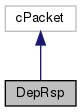
\includegraphics[width=133pt]{class_dep_rsp__inherit__graph}
\end{center}
\end{figure}


Collaboration diagram for Dep\+Rsp\+:\nopagebreak
\begin{figure}[H]
\begin{center}
\leavevmode
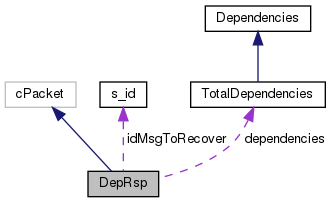
\includegraphics[width=321pt]{class_dep_rsp__coll__graph}
\end{center}
\end{figure}
\subsection*{Public Member Functions}
\begin{DoxyCompactItemize}
\item 
\hyperlink{class_dep_rsp_a86d6896d681e4467ec52c660738893ed}{Dep\+Rsp} (const char $\ast$name=nullptr, short kind=0)
\item 
\hyperlink{class_dep_rsp_a3b5894b34b151dced8080a6e5757c2a2}{Dep\+Rsp} (const \hyperlink{class_dep_rsp}{Dep\+Rsp} \&other)
\item 
virtual \hyperlink{class_dep_rsp_aa4c1e70c5fd15e5a9541b58999df3480}{$\sim$\+Dep\+Rsp} ()
\item 
\hyperlink{class_dep_rsp}{Dep\+Rsp} \& \hyperlink{class_dep_rsp_a3297f65b6eb05d7d5d203562b4d48c4a}{operator=} (const \hyperlink{class_dep_rsp}{Dep\+Rsp} \&other)
\item 
virtual \hyperlink{class_dep_rsp}{Dep\+Rsp} $\ast$ \hyperlink{class_dep_rsp_af70e467ce29aac0e865ac06c3a021019}{dup} () const override
\item 
virtual void \hyperlink{class_dep_rsp_a2125eed5bc70db3cc55e41e144c8716f}{parsim\+Pack} (omnetpp\+::c\+Comm\+Buffer $\ast$b) const override
\item 
virtual void \hyperlink{class_dep_rsp_a8d8d59c349898c4dfb9da1845ba0acdd}{parsim\+Unpack} (omnetpp\+::c\+Comm\+Buffer $\ast$b) override
\item 
virtual \hyperlink{dep_rsp__m_8h_a8a41011e0821f196429cd4bc45638bcf}{id\+Msg\+Dep\+Rsp} \& \hyperlink{class_dep_rsp_a7558f4f82be1ce27c894a068e2811ec6}{get\+Id\+Msg\+To\+Recover} ()
\item 
virtual const \hyperlink{dep_rsp__m_8h_a8a41011e0821f196429cd4bc45638bcf}{id\+Msg\+Dep\+Rsp} \& \hyperlink{class_dep_rsp_a209fe969214c0bf673d12a27bb923f92}{get\+Id\+Msg\+To\+Recover} () const
\item 
virtual void \hyperlink{class_dep_rsp_a6aea88bdf4ba7b9c4876823278e880b0}{set\+Id\+Msg\+To\+Recover} (const \hyperlink{dep_rsp__m_8h_a8a41011e0821f196429cd4bc45638bcf}{id\+Msg\+Dep\+Rsp} \&\hyperlink{class_dep_rsp_a7b777428e859ba7a6f083e13f6431cf4}{id\+Msg\+To\+Recover})
\item 
virtual \hyperlink{dep_rsp__m_8h_a3c2ceb107008eb344443aaab2eb872b8}{id\+Dep\+Dep\+Rsp} \& \hyperlink{class_dep_rsp_a507c1f42135deca6079b31f5fe8da301}{get\+Dependencies} ()
\item 
virtual const \hyperlink{dep_rsp__m_8h_a3c2ceb107008eb344443aaab2eb872b8}{id\+Dep\+Dep\+Rsp} \& \hyperlink{class_dep_rsp_ad7d207f5cb583e04c7a8a6127bcb3fff}{get\+Dependencies} () const
\item 
virtual void \hyperlink{class_dep_rsp_ab144b3866dd1a527842806ced90495f6}{set\+Dependencies} (const \hyperlink{dep_rsp__m_8h_a3c2ceb107008eb344443aaab2eb872b8}{id\+Dep\+Dep\+Rsp} \&\hyperlink{class_dep_rsp_a0881ee52098e202a4486da80efa6ce1f}{dependencies})
\item 
virtual \hyperlink{dep_rsp__m_8h_ab118b8474723cf26f98151aae3d55940}{dep\+Rsp\+Time} \& \hyperlink{class_dep_rsp_a89f0b26c269083713702386392f82c45}{get\+Delay} ()
\item 
virtual const \hyperlink{dep_rsp__m_8h_ab118b8474723cf26f98151aae3d55940}{dep\+Rsp\+Time} \& \hyperlink{class_dep_rsp_a8badf32e7f81c0ec7a9b4eb22fb83c0a}{get\+Delay} () const
\item 
virtual void \hyperlink{class_dep_rsp_a582682e76c175afb882cf50d2b423501}{set\+Delay} (const \hyperlink{dep_rsp__m_8h_ab118b8474723cf26f98151aae3d55940}{dep\+Rsp\+Time} \&\hyperlink{class_dep_rsp_a9b383b175e0b581e1558b2dc34a21b7a}{delay})
\item 
virtual unsigned int \hyperlink{class_dep_rsp_a3c858b0cb735e9e6309e8bf25bf272dd}{get\+Id\+Requster} () const
\item 
virtual void \hyperlink{class_dep_rsp_a7029f3c6f0e1b230965a0143a3c9724e}{set\+Id\+Requster} (unsigned int \hyperlink{class_dep_rsp_ae8c6f097db47049e4cb84e6788f9d58d}{id\+Requster})
\end{DoxyCompactItemize}
\subsection*{Protected Member Functions}
\begin{DoxyCompactItemize}
\item 
bool \hyperlink{class_dep_rsp_a4796a7a035aa6f4b9deb40498731a941}{operator==} (const \hyperlink{class_dep_rsp}{Dep\+Rsp} \&)
\end{DoxyCompactItemize}
\subsection*{Protected Attributes}
\begin{DoxyCompactItemize}
\item 
\hyperlink{dep_rsp__m_8h_a8a41011e0821f196429cd4bc45638bcf}{id\+Msg\+Dep\+Rsp} \hyperlink{class_dep_rsp_a7b777428e859ba7a6f083e13f6431cf4}{id\+Msg\+To\+Recover}
\item 
\hyperlink{dep_rsp__m_8h_a3c2ceb107008eb344443aaab2eb872b8}{id\+Dep\+Dep\+Rsp} \hyperlink{class_dep_rsp_a0881ee52098e202a4486da80efa6ce1f}{dependencies}
\item 
\hyperlink{dep_rsp__m_8h_ab118b8474723cf26f98151aae3d55940}{dep\+Rsp\+Time} \hyperlink{class_dep_rsp_a9b383b175e0b581e1558b2dc34a21b7a}{delay}
\item 
unsigned int \hyperlink{class_dep_rsp_ae8c6f097db47049e4cb84e6788f9d58d}{id\+Requster}
\end{DoxyCompactItemize}
\subsection*{Private Member Functions}
\begin{DoxyCompactItemize}
\item 
void \hyperlink{class_dep_rsp_ad8bf8a80dd4586392e1f5179b7b612f5}{copy} (const \hyperlink{class_dep_rsp}{Dep\+Rsp} \&other)
\end{DoxyCompactItemize}


\subsection{Detailed Description}
Class generated from {\ttfamily Messages/dep\+Rsp.\+msg\+:42} by nedtool. 


\begin{DoxyPre}
packet \hyperlink{class_dep_rsp}{DepRsp}
\{
    idMsgDepRsp idMsgToRecover;
    idDepDepRsp dependencies;
    depRspTime delay; // ms 
    unsigned int idRequster;
\}
\end{DoxyPre}
 

\subsection{Constructor \& Destructor Documentation}
\mbox{\Hypertarget{class_dep_rsp_a86d6896d681e4467ec52c660738893ed}\label{class_dep_rsp_a86d6896d681e4467ec52c660738893ed}} 
\index{Dep\+Rsp@{Dep\+Rsp}!Dep\+Rsp@{Dep\+Rsp}}
\index{Dep\+Rsp@{Dep\+Rsp}!Dep\+Rsp@{Dep\+Rsp}}
\subsubsection{\texorpdfstring{Dep\+Rsp()}{DepRsp()}\hspace{0.1cm}{\footnotesize\ttfamily [1/2]}}
{\footnotesize\ttfamily Dep\+Rsp\+::\+Dep\+Rsp (\begin{DoxyParamCaption}\item[{const char $\ast$}]{name = {\ttfamily nullptr},  }\item[{short}]{kind = {\ttfamily 0} }\end{DoxyParamCaption})}

\mbox{\Hypertarget{class_dep_rsp_a3b5894b34b151dced8080a6e5757c2a2}\label{class_dep_rsp_a3b5894b34b151dced8080a6e5757c2a2}} 
\index{Dep\+Rsp@{Dep\+Rsp}!Dep\+Rsp@{Dep\+Rsp}}
\index{Dep\+Rsp@{Dep\+Rsp}!Dep\+Rsp@{Dep\+Rsp}}
\subsubsection{\texorpdfstring{Dep\+Rsp()}{DepRsp()}\hspace{0.1cm}{\footnotesize\ttfamily [2/2]}}
{\footnotesize\ttfamily Dep\+Rsp\+::\+Dep\+Rsp (\begin{DoxyParamCaption}\item[{const \hyperlink{class_dep_rsp}{Dep\+Rsp} \&}]{other }\end{DoxyParamCaption})}

\mbox{\Hypertarget{class_dep_rsp_aa4c1e70c5fd15e5a9541b58999df3480}\label{class_dep_rsp_aa4c1e70c5fd15e5a9541b58999df3480}} 
\index{Dep\+Rsp@{Dep\+Rsp}!````~Dep\+Rsp@{$\sim$\+Dep\+Rsp}}
\index{````~Dep\+Rsp@{$\sim$\+Dep\+Rsp}!Dep\+Rsp@{Dep\+Rsp}}
\subsubsection{\texorpdfstring{$\sim$\+Dep\+Rsp()}{~DepRsp()}}
{\footnotesize\ttfamily Dep\+Rsp\+::$\sim$\+Dep\+Rsp (\begin{DoxyParamCaption}{ }\end{DoxyParamCaption})\hspace{0.3cm}{\ttfamily [virtual]}}



\subsection{Member Function Documentation}
\mbox{\Hypertarget{class_dep_rsp_ad8bf8a80dd4586392e1f5179b7b612f5}\label{class_dep_rsp_ad8bf8a80dd4586392e1f5179b7b612f5}} 
\index{Dep\+Rsp@{Dep\+Rsp}!copy@{copy}}
\index{copy@{copy}!Dep\+Rsp@{Dep\+Rsp}}
\subsubsection{\texorpdfstring{copy()}{copy()}}
{\footnotesize\ttfamily void Dep\+Rsp\+::copy (\begin{DoxyParamCaption}\item[{const \hyperlink{class_dep_rsp}{Dep\+Rsp} \&}]{other }\end{DoxyParamCaption})\hspace{0.3cm}{\ttfamily [private]}}

\mbox{\Hypertarget{class_dep_rsp_af70e467ce29aac0e865ac06c3a021019}\label{class_dep_rsp_af70e467ce29aac0e865ac06c3a021019}} 
\index{Dep\+Rsp@{Dep\+Rsp}!dup@{dup}}
\index{dup@{dup}!Dep\+Rsp@{Dep\+Rsp}}
\subsubsection{\texorpdfstring{dup()}{dup()}}
{\footnotesize\ttfamily virtual \hyperlink{class_dep_rsp}{Dep\+Rsp}$\ast$ Dep\+Rsp\+::dup (\begin{DoxyParamCaption}{ }\end{DoxyParamCaption}) const\hspace{0.3cm}{\ttfamily [inline]}, {\ttfamily [override]}, {\ttfamily [virtual]}}

\mbox{\Hypertarget{class_dep_rsp_a89f0b26c269083713702386392f82c45}\label{class_dep_rsp_a89f0b26c269083713702386392f82c45}} 
\index{Dep\+Rsp@{Dep\+Rsp}!get\+Delay@{get\+Delay}}
\index{get\+Delay@{get\+Delay}!Dep\+Rsp@{Dep\+Rsp}}
\subsubsection{\texorpdfstring{get\+Delay()}{getDelay()}\hspace{0.1cm}{\footnotesize\ttfamily [1/2]}}
{\footnotesize\ttfamily \hyperlink{dep_rsp__m_8h_ab118b8474723cf26f98151aae3d55940}{dep\+Rsp\+Time} \& Dep\+Rsp\+::get\+Delay (\begin{DoxyParamCaption}{ }\end{DoxyParamCaption})\hspace{0.3cm}{\ttfamily [virtual]}}

\mbox{\Hypertarget{class_dep_rsp_a8badf32e7f81c0ec7a9b4eb22fb83c0a}\label{class_dep_rsp_a8badf32e7f81c0ec7a9b4eb22fb83c0a}} 
\index{Dep\+Rsp@{Dep\+Rsp}!get\+Delay@{get\+Delay}}
\index{get\+Delay@{get\+Delay}!Dep\+Rsp@{Dep\+Rsp}}
\subsubsection{\texorpdfstring{get\+Delay()}{getDelay()}\hspace{0.1cm}{\footnotesize\ttfamily [2/2]}}
{\footnotesize\ttfamily virtual const \hyperlink{dep_rsp__m_8h_ab118b8474723cf26f98151aae3d55940}{dep\+Rsp\+Time}\& Dep\+Rsp\+::get\+Delay (\begin{DoxyParamCaption}{ }\end{DoxyParamCaption}) const\hspace{0.3cm}{\ttfamily [inline]}, {\ttfamily [virtual]}}

\mbox{\Hypertarget{class_dep_rsp_a507c1f42135deca6079b31f5fe8da301}\label{class_dep_rsp_a507c1f42135deca6079b31f5fe8da301}} 
\index{Dep\+Rsp@{Dep\+Rsp}!get\+Dependencies@{get\+Dependencies}}
\index{get\+Dependencies@{get\+Dependencies}!Dep\+Rsp@{Dep\+Rsp}}
\subsubsection{\texorpdfstring{get\+Dependencies()}{getDependencies()}\hspace{0.1cm}{\footnotesize\ttfamily [1/2]}}
{\footnotesize\ttfamily \hyperlink{dep_rsp__m_8h_a3c2ceb107008eb344443aaab2eb872b8}{id\+Dep\+Dep\+Rsp} \& Dep\+Rsp\+::get\+Dependencies (\begin{DoxyParamCaption}{ }\end{DoxyParamCaption})\hspace{0.3cm}{\ttfamily [virtual]}}

\mbox{\Hypertarget{class_dep_rsp_ad7d207f5cb583e04c7a8a6127bcb3fff}\label{class_dep_rsp_ad7d207f5cb583e04c7a8a6127bcb3fff}} 
\index{Dep\+Rsp@{Dep\+Rsp}!get\+Dependencies@{get\+Dependencies}}
\index{get\+Dependencies@{get\+Dependencies}!Dep\+Rsp@{Dep\+Rsp}}
\subsubsection{\texorpdfstring{get\+Dependencies()}{getDependencies()}\hspace{0.1cm}{\footnotesize\ttfamily [2/2]}}
{\footnotesize\ttfamily virtual const \hyperlink{dep_rsp__m_8h_a3c2ceb107008eb344443aaab2eb872b8}{id\+Dep\+Dep\+Rsp}\& Dep\+Rsp\+::get\+Dependencies (\begin{DoxyParamCaption}{ }\end{DoxyParamCaption}) const\hspace{0.3cm}{\ttfamily [inline]}, {\ttfamily [virtual]}}

\mbox{\Hypertarget{class_dep_rsp_a7558f4f82be1ce27c894a068e2811ec6}\label{class_dep_rsp_a7558f4f82be1ce27c894a068e2811ec6}} 
\index{Dep\+Rsp@{Dep\+Rsp}!get\+Id\+Msg\+To\+Recover@{get\+Id\+Msg\+To\+Recover}}
\index{get\+Id\+Msg\+To\+Recover@{get\+Id\+Msg\+To\+Recover}!Dep\+Rsp@{Dep\+Rsp}}
\subsubsection{\texorpdfstring{get\+Id\+Msg\+To\+Recover()}{getIdMsgToRecover()}\hspace{0.1cm}{\footnotesize\ttfamily [1/2]}}
{\footnotesize\ttfamily \hyperlink{dep_rsp__m_8h_a8a41011e0821f196429cd4bc45638bcf}{id\+Msg\+Dep\+Rsp} \& Dep\+Rsp\+::get\+Id\+Msg\+To\+Recover (\begin{DoxyParamCaption}{ }\end{DoxyParamCaption})\hspace{0.3cm}{\ttfamily [virtual]}}

\mbox{\Hypertarget{class_dep_rsp_a209fe969214c0bf673d12a27bb923f92}\label{class_dep_rsp_a209fe969214c0bf673d12a27bb923f92}} 
\index{Dep\+Rsp@{Dep\+Rsp}!get\+Id\+Msg\+To\+Recover@{get\+Id\+Msg\+To\+Recover}}
\index{get\+Id\+Msg\+To\+Recover@{get\+Id\+Msg\+To\+Recover}!Dep\+Rsp@{Dep\+Rsp}}
\subsubsection{\texorpdfstring{get\+Id\+Msg\+To\+Recover()}{getIdMsgToRecover()}\hspace{0.1cm}{\footnotesize\ttfamily [2/2]}}
{\footnotesize\ttfamily virtual const \hyperlink{dep_rsp__m_8h_a8a41011e0821f196429cd4bc45638bcf}{id\+Msg\+Dep\+Rsp}\& Dep\+Rsp\+::get\+Id\+Msg\+To\+Recover (\begin{DoxyParamCaption}{ }\end{DoxyParamCaption}) const\hspace{0.3cm}{\ttfamily [inline]}, {\ttfamily [virtual]}}

\mbox{\Hypertarget{class_dep_rsp_a3c858b0cb735e9e6309e8bf25bf272dd}\label{class_dep_rsp_a3c858b0cb735e9e6309e8bf25bf272dd}} 
\index{Dep\+Rsp@{Dep\+Rsp}!get\+Id\+Requster@{get\+Id\+Requster}}
\index{get\+Id\+Requster@{get\+Id\+Requster}!Dep\+Rsp@{Dep\+Rsp}}
\subsubsection{\texorpdfstring{get\+Id\+Requster()}{getIdRequster()}}
{\footnotesize\ttfamily unsigned int Dep\+Rsp\+::get\+Id\+Requster (\begin{DoxyParamCaption}{ }\end{DoxyParamCaption}) const\hspace{0.3cm}{\ttfamily [virtual]}}

\mbox{\Hypertarget{class_dep_rsp_a3297f65b6eb05d7d5d203562b4d48c4a}\label{class_dep_rsp_a3297f65b6eb05d7d5d203562b4d48c4a}} 
\index{Dep\+Rsp@{Dep\+Rsp}!operator=@{operator=}}
\index{operator=@{operator=}!Dep\+Rsp@{Dep\+Rsp}}
\subsubsection{\texorpdfstring{operator=()}{operator=()}}
{\footnotesize\ttfamily \hyperlink{class_dep_rsp}{Dep\+Rsp} \& Dep\+Rsp\+::operator= (\begin{DoxyParamCaption}\item[{const \hyperlink{class_dep_rsp}{Dep\+Rsp} \&}]{other }\end{DoxyParamCaption})}

\mbox{\Hypertarget{class_dep_rsp_a4796a7a035aa6f4b9deb40498731a941}\label{class_dep_rsp_a4796a7a035aa6f4b9deb40498731a941}} 
\index{Dep\+Rsp@{Dep\+Rsp}!operator==@{operator==}}
\index{operator==@{operator==}!Dep\+Rsp@{Dep\+Rsp}}
\subsubsection{\texorpdfstring{operator==()}{operator==()}}
{\footnotesize\ttfamily bool Dep\+Rsp\+::operator== (\begin{DoxyParamCaption}\item[{const \hyperlink{class_dep_rsp}{Dep\+Rsp} \&}]{ }\end{DoxyParamCaption})\hspace{0.3cm}{\ttfamily [protected]}}

\mbox{\Hypertarget{class_dep_rsp_a2125eed5bc70db3cc55e41e144c8716f}\label{class_dep_rsp_a2125eed5bc70db3cc55e41e144c8716f}} 
\index{Dep\+Rsp@{Dep\+Rsp}!parsim\+Pack@{parsim\+Pack}}
\index{parsim\+Pack@{parsim\+Pack}!Dep\+Rsp@{Dep\+Rsp}}
\subsubsection{\texorpdfstring{parsim\+Pack()}{parsimPack()}}
{\footnotesize\ttfamily void Dep\+Rsp\+::parsim\+Pack (\begin{DoxyParamCaption}\item[{omnetpp\+::c\+Comm\+Buffer $\ast$}]{b }\end{DoxyParamCaption}) const\hspace{0.3cm}{\ttfamily [override]}, {\ttfamily [virtual]}}

\mbox{\Hypertarget{class_dep_rsp_a8d8d59c349898c4dfb9da1845ba0acdd}\label{class_dep_rsp_a8d8d59c349898c4dfb9da1845ba0acdd}} 
\index{Dep\+Rsp@{Dep\+Rsp}!parsim\+Unpack@{parsim\+Unpack}}
\index{parsim\+Unpack@{parsim\+Unpack}!Dep\+Rsp@{Dep\+Rsp}}
\subsubsection{\texorpdfstring{parsim\+Unpack()}{parsimUnpack()}}
{\footnotesize\ttfamily void Dep\+Rsp\+::parsim\+Unpack (\begin{DoxyParamCaption}\item[{omnetpp\+::c\+Comm\+Buffer $\ast$}]{b }\end{DoxyParamCaption})\hspace{0.3cm}{\ttfamily [override]}, {\ttfamily [virtual]}}

\mbox{\Hypertarget{class_dep_rsp_a582682e76c175afb882cf50d2b423501}\label{class_dep_rsp_a582682e76c175afb882cf50d2b423501}} 
\index{Dep\+Rsp@{Dep\+Rsp}!set\+Delay@{set\+Delay}}
\index{set\+Delay@{set\+Delay}!Dep\+Rsp@{Dep\+Rsp}}
\subsubsection{\texorpdfstring{set\+Delay()}{setDelay()}}
{\footnotesize\ttfamily void Dep\+Rsp\+::set\+Delay (\begin{DoxyParamCaption}\item[{const \hyperlink{dep_rsp__m_8h_ab118b8474723cf26f98151aae3d55940}{dep\+Rsp\+Time} \&}]{delay }\end{DoxyParamCaption})\hspace{0.3cm}{\ttfamily [virtual]}}

\mbox{\Hypertarget{class_dep_rsp_ab144b3866dd1a527842806ced90495f6}\label{class_dep_rsp_ab144b3866dd1a527842806ced90495f6}} 
\index{Dep\+Rsp@{Dep\+Rsp}!set\+Dependencies@{set\+Dependencies}}
\index{set\+Dependencies@{set\+Dependencies}!Dep\+Rsp@{Dep\+Rsp}}
\subsubsection{\texorpdfstring{set\+Dependencies()}{setDependencies()}}
{\footnotesize\ttfamily void Dep\+Rsp\+::set\+Dependencies (\begin{DoxyParamCaption}\item[{const \hyperlink{dep_rsp__m_8h_a3c2ceb107008eb344443aaab2eb872b8}{id\+Dep\+Dep\+Rsp} \&}]{dependencies }\end{DoxyParamCaption})\hspace{0.3cm}{\ttfamily [virtual]}}

\mbox{\Hypertarget{class_dep_rsp_a6aea88bdf4ba7b9c4876823278e880b0}\label{class_dep_rsp_a6aea88bdf4ba7b9c4876823278e880b0}} 
\index{Dep\+Rsp@{Dep\+Rsp}!set\+Id\+Msg\+To\+Recover@{set\+Id\+Msg\+To\+Recover}}
\index{set\+Id\+Msg\+To\+Recover@{set\+Id\+Msg\+To\+Recover}!Dep\+Rsp@{Dep\+Rsp}}
\subsubsection{\texorpdfstring{set\+Id\+Msg\+To\+Recover()}{setIdMsgToRecover()}}
{\footnotesize\ttfamily void Dep\+Rsp\+::set\+Id\+Msg\+To\+Recover (\begin{DoxyParamCaption}\item[{const \hyperlink{dep_rsp__m_8h_a8a41011e0821f196429cd4bc45638bcf}{id\+Msg\+Dep\+Rsp} \&}]{id\+Msg\+To\+Recover }\end{DoxyParamCaption})\hspace{0.3cm}{\ttfamily [virtual]}}

\mbox{\Hypertarget{class_dep_rsp_a7029f3c6f0e1b230965a0143a3c9724e}\label{class_dep_rsp_a7029f3c6f0e1b230965a0143a3c9724e}} 
\index{Dep\+Rsp@{Dep\+Rsp}!set\+Id\+Requster@{set\+Id\+Requster}}
\index{set\+Id\+Requster@{set\+Id\+Requster}!Dep\+Rsp@{Dep\+Rsp}}
\subsubsection{\texorpdfstring{set\+Id\+Requster()}{setIdRequster()}}
{\footnotesize\ttfamily void Dep\+Rsp\+::set\+Id\+Requster (\begin{DoxyParamCaption}\item[{unsigned int}]{id\+Requster }\end{DoxyParamCaption})\hspace{0.3cm}{\ttfamily [virtual]}}



\subsection{Member Data Documentation}
\mbox{\Hypertarget{class_dep_rsp_a9b383b175e0b581e1558b2dc34a21b7a}\label{class_dep_rsp_a9b383b175e0b581e1558b2dc34a21b7a}} 
\index{Dep\+Rsp@{Dep\+Rsp}!delay@{delay}}
\index{delay@{delay}!Dep\+Rsp@{Dep\+Rsp}}
\subsubsection{\texorpdfstring{delay}{delay}}
{\footnotesize\ttfamily \hyperlink{dep_rsp__m_8h_ab118b8474723cf26f98151aae3d55940}{dep\+Rsp\+Time} Dep\+Rsp\+::delay\hspace{0.3cm}{\ttfamily [protected]}}

\mbox{\Hypertarget{class_dep_rsp_a0881ee52098e202a4486da80efa6ce1f}\label{class_dep_rsp_a0881ee52098e202a4486da80efa6ce1f}} 
\index{Dep\+Rsp@{Dep\+Rsp}!dependencies@{dependencies}}
\index{dependencies@{dependencies}!Dep\+Rsp@{Dep\+Rsp}}
\subsubsection{\texorpdfstring{dependencies}{dependencies}}
{\footnotesize\ttfamily \hyperlink{dep_rsp__m_8h_a3c2ceb107008eb344443aaab2eb872b8}{id\+Dep\+Dep\+Rsp} Dep\+Rsp\+::dependencies\hspace{0.3cm}{\ttfamily [protected]}}

\mbox{\Hypertarget{class_dep_rsp_a7b777428e859ba7a6f083e13f6431cf4}\label{class_dep_rsp_a7b777428e859ba7a6f083e13f6431cf4}} 
\index{Dep\+Rsp@{Dep\+Rsp}!id\+Msg\+To\+Recover@{id\+Msg\+To\+Recover}}
\index{id\+Msg\+To\+Recover@{id\+Msg\+To\+Recover}!Dep\+Rsp@{Dep\+Rsp}}
\subsubsection{\texorpdfstring{id\+Msg\+To\+Recover}{idMsgToRecover}}
{\footnotesize\ttfamily \hyperlink{dep_rsp__m_8h_a8a41011e0821f196429cd4bc45638bcf}{id\+Msg\+Dep\+Rsp} Dep\+Rsp\+::id\+Msg\+To\+Recover\hspace{0.3cm}{\ttfamily [protected]}}

\mbox{\Hypertarget{class_dep_rsp_ae8c6f097db47049e4cb84e6788f9d58d}\label{class_dep_rsp_ae8c6f097db47049e4cb84e6788f9d58d}} 
\index{Dep\+Rsp@{Dep\+Rsp}!id\+Requster@{id\+Requster}}
\index{id\+Requster@{id\+Requster}!Dep\+Rsp@{Dep\+Rsp}}
\subsubsection{\texorpdfstring{id\+Requster}{idRequster}}
{\footnotesize\ttfamily unsigned int Dep\+Rsp\+::id\+Requster\hspace{0.3cm}{\ttfamily [protected]}}



The documentation for this class was generated from the following files\+:\begin{DoxyCompactItemize}
\item 
src/\+Messages/\hyperlink{dep_rsp__m_8h}{dep\+Rsp\+\_\+m.\+h}\item 
src/\+Messages/\hyperlink{dep_rsp__m_8cc}{dep\+Rsp\+\_\+m.\+cc}\end{DoxyCompactItemize}

\hypertarget{class_dep_rsp_descriptor}{}\section{Dep\+Rsp\+Descriptor Class Reference}
\label{class_dep_rsp_descriptor}\index{Dep\+Rsp\+Descriptor@{Dep\+Rsp\+Descriptor}}


Inheritance diagram for Dep\+Rsp\+Descriptor\+:\nopagebreak
\begin{figure}[H]
\begin{center}
\leavevmode
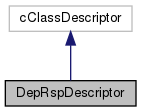
\includegraphics[width=178pt]{class_dep_rsp_descriptor__inherit__graph}
\end{center}
\end{figure}


Collaboration diagram for Dep\+Rsp\+Descriptor\+:\nopagebreak
\begin{figure}[H]
\begin{center}
\leavevmode
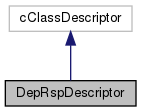
\includegraphics[width=178pt]{class_dep_rsp_descriptor__coll__graph}
\end{center}
\end{figure}
\subsection*{Public Member Functions}
\begin{DoxyCompactItemize}
\item 
\hyperlink{class_dep_rsp_descriptor_ad256a6a63460351ea6a372618915c2d8}{Dep\+Rsp\+Descriptor} ()
\item 
virtual \hyperlink{class_dep_rsp_descriptor_abc19e536e455faeb3fd8670b5447a083}{$\sim$\+Dep\+Rsp\+Descriptor} ()
\item 
virtual bool \hyperlink{class_dep_rsp_descriptor_a7a880007ffa97b1e7506e5006dff76fc}{does\+Support} (omnetpp\+::c\+Object $\ast$obj) const override
\item 
virtual const char $\ast$$\ast$ \hyperlink{class_dep_rsp_descriptor_a9549506315f1c8710721599924afec0d}{get\+Property\+Names} () const override
\item 
virtual const char $\ast$ \hyperlink{class_dep_rsp_descriptor_aafacdcf48c89777dd32b2515d46156a3}{get\+Property} (const char $\ast$propertyname) const override
\item 
virtual int \hyperlink{class_dep_rsp_descriptor_a7704deff767464de71b08e877144aef3}{get\+Field\+Count} () const override
\item 
virtual const char $\ast$ \hyperlink{class_dep_rsp_descriptor_a7ae3b3dbb2acbc29d3e6b9d80dad5f42}{get\+Field\+Name} (int field) const override
\item 
virtual int \hyperlink{class_dep_rsp_descriptor_a585faf6892da7b79d18edde57949fcc6}{find\+Field} (const char $\ast$field\+Name) const override
\item 
virtual unsigned int \hyperlink{class_dep_rsp_descriptor_a1d2e200ee36fc4be43c1babc7b1b4a19}{get\+Field\+Type\+Flags} (int field) const override
\item 
virtual const char $\ast$ \hyperlink{class_dep_rsp_descriptor_a2886a2c8ff88687682793f94abeee31b}{get\+Field\+Type\+String} (int field) const override
\item 
virtual const char $\ast$$\ast$ \hyperlink{class_dep_rsp_descriptor_ae59e1248d631d86bbec3d02c5cd03db8}{get\+Field\+Property\+Names} (int field) const override
\item 
virtual const char $\ast$ \hyperlink{class_dep_rsp_descriptor_a8cf738132398ab2204904ed1388fcd40}{get\+Field\+Property} (int field, const char $\ast$propertyname) const override
\item 
virtual int \hyperlink{class_dep_rsp_descriptor_a559a24842bd0a622463eb3417a31fc5c}{get\+Field\+Array\+Size} (void $\ast$object, int field) const override
\item 
virtual const char $\ast$ \hyperlink{class_dep_rsp_descriptor_ad838a8750347f561ed11e90b256aeb22}{get\+Field\+Dynamic\+Type\+String} (void $\ast$object, int field, int i) const override
\item 
virtual std\+::string \hyperlink{class_dep_rsp_descriptor_a026817a85cc05c7437c2a268a1829904}{get\+Field\+Value\+As\+String} (void $\ast$object, int field, int i) const override
\item 
virtual bool \hyperlink{class_dep_rsp_descriptor_a3414d7eb627262e4a5a99c30c1576f8f}{set\+Field\+Value\+As\+String} (void $\ast$object, int field, int i, const char $\ast$value) const override
\item 
virtual const char $\ast$ \hyperlink{class_dep_rsp_descriptor_a0cd988268afab355cb362d4b00e85a33}{get\+Field\+Struct\+Name} (int field) const override
\item 
virtual void $\ast$ \hyperlink{class_dep_rsp_descriptor_a08b3228538e6111c6f337ead9abbf557}{get\+Field\+Struct\+Value\+Pointer} (void $\ast$object, int field, int i) const override
\end{DoxyCompactItemize}
\subsection*{Private Attributes}
\begin{DoxyCompactItemize}
\item 
const char $\ast$$\ast$ \hyperlink{class_dep_rsp_descriptor_a496616950826cf009074023668b335de}{propertynames}
\end{DoxyCompactItemize}


\subsection{Constructor \& Destructor Documentation}
\mbox{\Hypertarget{class_dep_rsp_descriptor_ad256a6a63460351ea6a372618915c2d8}\label{class_dep_rsp_descriptor_ad256a6a63460351ea6a372618915c2d8}} 
\index{Dep\+Rsp\+Descriptor@{Dep\+Rsp\+Descriptor}!Dep\+Rsp\+Descriptor@{Dep\+Rsp\+Descriptor}}
\index{Dep\+Rsp\+Descriptor@{Dep\+Rsp\+Descriptor}!Dep\+Rsp\+Descriptor@{Dep\+Rsp\+Descriptor}}
\subsubsection{\texorpdfstring{Dep\+Rsp\+Descriptor()}{DepRspDescriptor()}}
{\footnotesize\ttfamily Dep\+Rsp\+Descriptor\+::\+Dep\+Rsp\+Descriptor (\begin{DoxyParamCaption}{ }\end{DoxyParamCaption})}

\mbox{\Hypertarget{class_dep_rsp_descriptor_abc19e536e455faeb3fd8670b5447a083}\label{class_dep_rsp_descriptor_abc19e536e455faeb3fd8670b5447a083}} 
\index{Dep\+Rsp\+Descriptor@{Dep\+Rsp\+Descriptor}!````~Dep\+Rsp\+Descriptor@{$\sim$\+Dep\+Rsp\+Descriptor}}
\index{````~Dep\+Rsp\+Descriptor@{$\sim$\+Dep\+Rsp\+Descriptor}!Dep\+Rsp\+Descriptor@{Dep\+Rsp\+Descriptor}}
\subsubsection{\texorpdfstring{$\sim$\+Dep\+Rsp\+Descriptor()}{~DepRspDescriptor()}}
{\footnotesize\ttfamily Dep\+Rsp\+Descriptor\+::$\sim$\+Dep\+Rsp\+Descriptor (\begin{DoxyParamCaption}{ }\end{DoxyParamCaption})\hspace{0.3cm}{\ttfamily [virtual]}}



\subsection{Member Function Documentation}
\mbox{\Hypertarget{class_dep_rsp_descriptor_a7a880007ffa97b1e7506e5006dff76fc}\label{class_dep_rsp_descriptor_a7a880007ffa97b1e7506e5006dff76fc}} 
\index{Dep\+Rsp\+Descriptor@{Dep\+Rsp\+Descriptor}!does\+Support@{does\+Support}}
\index{does\+Support@{does\+Support}!Dep\+Rsp\+Descriptor@{Dep\+Rsp\+Descriptor}}
\subsubsection{\texorpdfstring{does\+Support()}{doesSupport()}}
{\footnotesize\ttfamily bool Dep\+Rsp\+Descriptor\+::does\+Support (\begin{DoxyParamCaption}\item[{omnetpp\+::c\+Object $\ast$}]{obj }\end{DoxyParamCaption}) const\hspace{0.3cm}{\ttfamily [override]}, {\ttfamily [virtual]}}

\mbox{\Hypertarget{class_dep_rsp_descriptor_a585faf6892da7b79d18edde57949fcc6}\label{class_dep_rsp_descriptor_a585faf6892da7b79d18edde57949fcc6}} 
\index{Dep\+Rsp\+Descriptor@{Dep\+Rsp\+Descriptor}!find\+Field@{find\+Field}}
\index{find\+Field@{find\+Field}!Dep\+Rsp\+Descriptor@{Dep\+Rsp\+Descriptor}}
\subsubsection{\texorpdfstring{find\+Field()}{findField()}}
{\footnotesize\ttfamily int Dep\+Rsp\+Descriptor\+::find\+Field (\begin{DoxyParamCaption}\item[{const char $\ast$}]{field\+Name }\end{DoxyParamCaption}) const\hspace{0.3cm}{\ttfamily [override]}, {\ttfamily [virtual]}}

\mbox{\Hypertarget{class_dep_rsp_descriptor_a559a24842bd0a622463eb3417a31fc5c}\label{class_dep_rsp_descriptor_a559a24842bd0a622463eb3417a31fc5c}} 
\index{Dep\+Rsp\+Descriptor@{Dep\+Rsp\+Descriptor}!get\+Field\+Array\+Size@{get\+Field\+Array\+Size}}
\index{get\+Field\+Array\+Size@{get\+Field\+Array\+Size}!Dep\+Rsp\+Descriptor@{Dep\+Rsp\+Descriptor}}
\subsubsection{\texorpdfstring{get\+Field\+Array\+Size()}{getFieldArraySize()}}
{\footnotesize\ttfamily int Dep\+Rsp\+Descriptor\+::get\+Field\+Array\+Size (\begin{DoxyParamCaption}\item[{void $\ast$}]{object,  }\item[{int}]{field }\end{DoxyParamCaption}) const\hspace{0.3cm}{\ttfamily [override]}, {\ttfamily [virtual]}}

\mbox{\Hypertarget{class_dep_rsp_descriptor_a7704deff767464de71b08e877144aef3}\label{class_dep_rsp_descriptor_a7704deff767464de71b08e877144aef3}} 
\index{Dep\+Rsp\+Descriptor@{Dep\+Rsp\+Descriptor}!get\+Field\+Count@{get\+Field\+Count}}
\index{get\+Field\+Count@{get\+Field\+Count}!Dep\+Rsp\+Descriptor@{Dep\+Rsp\+Descriptor}}
\subsubsection{\texorpdfstring{get\+Field\+Count()}{getFieldCount()}}
{\footnotesize\ttfamily int Dep\+Rsp\+Descriptor\+::get\+Field\+Count (\begin{DoxyParamCaption}{ }\end{DoxyParamCaption}) const\hspace{0.3cm}{\ttfamily [override]}, {\ttfamily [virtual]}}

\mbox{\Hypertarget{class_dep_rsp_descriptor_ad838a8750347f561ed11e90b256aeb22}\label{class_dep_rsp_descriptor_ad838a8750347f561ed11e90b256aeb22}} 
\index{Dep\+Rsp\+Descriptor@{Dep\+Rsp\+Descriptor}!get\+Field\+Dynamic\+Type\+String@{get\+Field\+Dynamic\+Type\+String}}
\index{get\+Field\+Dynamic\+Type\+String@{get\+Field\+Dynamic\+Type\+String}!Dep\+Rsp\+Descriptor@{Dep\+Rsp\+Descriptor}}
\subsubsection{\texorpdfstring{get\+Field\+Dynamic\+Type\+String()}{getFieldDynamicTypeString()}}
{\footnotesize\ttfamily const char $\ast$ Dep\+Rsp\+Descriptor\+::get\+Field\+Dynamic\+Type\+String (\begin{DoxyParamCaption}\item[{void $\ast$}]{object,  }\item[{int}]{field,  }\item[{int}]{i }\end{DoxyParamCaption}) const\hspace{0.3cm}{\ttfamily [override]}, {\ttfamily [virtual]}}

\mbox{\Hypertarget{class_dep_rsp_descriptor_a7ae3b3dbb2acbc29d3e6b9d80dad5f42}\label{class_dep_rsp_descriptor_a7ae3b3dbb2acbc29d3e6b9d80dad5f42}} 
\index{Dep\+Rsp\+Descriptor@{Dep\+Rsp\+Descriptor}!get\+Field\+Name@{get\+Field\+Name}}
\index{get\+Field\+Name@{get\+Field\+Name}!Dep\+Rsp\+Descriptor@{Dep\+Rsp\+Descriptor}}
\subsubsection{\texorpdfstring{get\+Field\+Name()}{getFieldName()}}
{\footnotesize\ttfamily const char $\ast$ Dep\+Rsp\+Descriptor\+::get\+Field\+Name (\begin{DoxyParamCaption}\item[{int}]{field }\end{DoxyParamCaption}) const\hspace{0.3cm}{\ttfamily [override]}, {\ttfamily [virtual]}}

\mbox{\Hypertarget{class_dep_rsp_descriptor_a8cf738132398ab2204904ed1388fcd40}\label{class_dep_rsp_descriptor_a8cf738132398ab2204904ed1388fcd40}} 
\index{Dep\+Rsp\+Descriptor@{Dep\+Rsp\+Descriptor}!get\+Field\+Property@{get\+Field\+Property}}
\index{get\+Field\+Property@{get\+Field\+Property}!Dep\+Rsp\+Descriptor@{Dep\+Rsp\+Descriptor}}
\subsubsection{\texorpdfstring{get\+Field\+Property()}{getFieldProperty()}}
{\footnotesize\ttfamily const char $\ast$ Dep\+Rsp\+Descriptor\+::get\+Field\+Property (\begin{DoxyParamCaption}\item[{int}]{field,  }\item[{const char $\ast$}]{propertyname }\end{DoxyParamCaption}) const\hspace{0.3cm}{\ttfamily [override]}, {\ttfamily [virtual]}}

\mbox{\Hypertarget{class_dep_rsp_descriptor_ae59e1248d631d86bbec3d02c5cd03db8}\label{class_dep_rsp_descriptor_ae59e1248d631d86bbec3d02c5cd03db8}} 
\index{Dep\+Rsp\+Descriptor@{Dep\+Rsp\+Descriptor}!get\+Field\+Property\+Names@{get\+Field\+Property\+Names}}
\index{get\+Field\+Property\+Names@{get\+Field\+Property\+Names}!Dep\+Rsp\+Descriptor@{Dep\+Rsp\+Descriptor}}
\subsubsection{\texorpdfstring{get\+Field\+Property\+Names()}{getFieldPropertyNames()}}
{\footnotesize\ttfamily const char $\ast$$\ast$ Dep\+Rsp\+Descriptor\+::get\+Field\+Property\+Names (\begin{DoxyParamCaption}\item[{int}]{field }\end{DoxyParamCaption}) const\hspace{0.3cm}{\ttfamily [override]}, {\ttfamily [virtual]}}

\mbox{\Hypertarget{class_dep_rsp_descriptor_a0cd988268afab355cb362d4b00e85a33}\label{class_dep_rsp_descriptor_a0cd988268afab355cb362d4b00e85a33}} 
\index{Dep\+Rsp\+Descriptor@{Dep\+Rsp\+Descriptor}!get\+Field\+Struct\+Name@{get\+Field\+Struct\+Name}}
\index{get\+Field\+Struct\+Name@{get\+Field\+Struct\+Name}!Dep\+Rsp\+Descriptor@{Dep\+Rsp\+Descriptor}}
\subsubsection{\texorpdfstring{get\+Field\+Struct\+Name()}{getFieldStructName()}}
{\footnotesize\ttfamily const char $\ast$ Dep\+Rsp\+Descriptor\+::get\+Field\+Struct\+Name (\begin{DoxyParamCaption}\item[{int}]{field }\end{DoxyParamCaption}) const\hspace{0.3cm}{\ttfamily [override]}, {\ttfamily [virtual]}}

\mbox{\Hypertarget{class_dep_rsp_descriptor_a08b3228538e6111c6f337ead9abbf557}\label{class_dep_rsp_descriptor_a08b3228538e6111c6f337ead9abbf557}} 
\index{Dep\+Rsp\+Descriptor@{Dep\+Rsp\+Descriptor}!get\+Field\+Struct\+Value\+Pointer@{get\+Field\+Struct\+Value\+Pointer}}
\index{get\+Field\+Struct\+Value\+Pointer@{get\+Field\+Struct\+Value\+Pointer}!Dep\+Rsp\+Descriptor@{Dep\+Rsp\+Descriptor}}
\subsubsection{\texorpdfstring{get\+Field\+Struct\+Value\+Pointer()}{getFieldStructValuePointer()}}
{\footnotesize\ttfamily void $\ast$ Dep\+Rsp\+Descriptor\+::get\+Field\+Struct\+Value\+Pointer (\begin{DoxyParamCaption}\item[{void $\ast$}]{object,  }\item[{int}]{field,  }\item[{int}]{i }\end{DoxyParamCaption}) const\hspace{0.3cm}{\ttfamily [override]}, {\ttfamily [virtual]}}

\mbox{\Hypertarget{class_dep_rsp_descriptor_a1d2e200ee36fc4be43c1babc7b1b4a19}\label{class_dep_rsp_descriptor_a1d2e200ee36fc4be43c1babc7b1b4a19}} 
\index{Dep\+Rsp\+Descriptor@{Dep\+Rsp\+Descriptor}!get\+Field\+Type\+Flags@{get\+Field\+Type\+Flags}}
\index{get\+Field\+Type\+Flags@{get\+Field\+Type\+Flags}!Dep\+Rsp\+Descriptor@{Dep\+Rsp\+Descriptor}}
\subsubsection{\texorpdfstring{get\+Field\+Type\+Flags()}{getFieldTypeFlags()}}
{\footnotesize\ttfamily unsigned int Dep\+Rsp\+Descriptor\+::get\+Field\+Type\+Flags (\begin{DoxyParamCaption}\item[{int}]{field }\end{DoxyParamCaption}) const\hspace{0.3cm}{\ttfamily [override]}, {\ttfamily [virtual]}}

\mbox{\Hypertarget{class_dep_rsp_descriptor_a2886a2c8ff88687682793f94abeee31b}\label{class_dep_rsp_descriptor_a2886a2c8ff88687682793f94abeee31b}} 
\index{Dep\+Rsp\+Descriptor@{Dep\+Rsp\+Descriptor}!get\+Field\+Type\+String@{get\+Field\+Type\+String}}
\index{get\+Field\+Type\+String@{get\+Field\+Type\+String}!Dep\+Rsp\+Descriptor@{Dep\+Rsp\+Descriptor}}
\subsubsection{\texorpdfstring{get\+Field\+Type\+String()}{getFieldTypeString()}}
{\footnotesize\ttfamily const char $\ast$ Dep\+Rsp\+Descriptor\+::get\+Field\+Type\+String (\begin{DoxyParamCaption}\item[{int}]{field }\end{DoxyParamCaption}) const\hspace{0.3cm}{\ttfamily [override]}, {\ttfamily [virtual]}}

\mbox{\Hypertarget{class_dep_rsp_descriptor_a026817a85cc05c7437c2a268a1829904}\label{class_dep_rsp_descriptor_a026817a85cc05c7437c2a268a1829904}} 
\index{Dep\+Rsp\+Descriptor@{Dep\+Rsp\+Descriptor}!get\+Field\+Value\+As\+String@{get\+Field\+Value\+As\+String}}
\index{get\+Field\+Value\+As\+String@{get\+Field\+Value\+As\+String}!Dep\+Rsp\+Descriptor@{Dep\+Rsp\+Descriptor}}
\subsubsection{\texorpdfstring{get\+Field\+Value\+As\+String()}{getFieldValueAsString()}}
{\footnotesize\ttfamily std\+::string Dep\+Rsp\+Descriptor\+::get\+Field\+Value\+As\+String (\begin{DoxyParamCaption}\item[{void $\ast$}]{object,  }\item[{int}]{field,  }\item[{int}]{i }\end{DoxyParamCaption}) const\hspace{0.3cm}{\ttfamily [override]}, {\ttfamily [virtual]}}

\mbox{\Hypertarget{class_dep_rsp_descriptor_aafacdcf48c89777dd32b2515d46156a3}\label{class_dep_rsp_descriptor_aafacdcf48c89777dd32b2515d46156a3}} 
\index{Dep\+Rsp\+Descriptor@{Dep\+Rsp\+Descriptor}!get\+Property@{get\+Property}}
\index{get\+Property@{get\+Property}!Dep\+Rsp\+Descriptor@{Dep\+Rsp\+Descriptor}}
\subsubsection{\texorpdfstring{get\+Property()}{getProperty()}}
{\footnotesize\ttfamily const char $\ast$ Dep\+Rsp\+Descriptor\+::get\+Property (\begin{DoxyParamCaption}\item[{const char $\ast$}]{propertyname }\end{DoxyParamCaption}) const\hspace{0.3cm}{\ttfamily [override]}, {\ttfamily [virtual]}}

\mbox{\Hypertarget{class_dep_rsp_descriptor_a9549506315f1c8710721599924afec0d}\label{class_dep_rsp_descriptor_a9549506315f1c8710721599924afec0d}} 
\index{Dep\+Rsp\+Descriptor@{Dep\+Rsp\+Descriptor}!get\+Property\+Names@{get\+Property\+Names}}
\index{get\+Property\+Names@{get\+Property\+Names}!Dep\+Rsp\+Descriptor@{Dep\+Rsp\+Descriptor}}
\subsubsection{\texorpdfstring{get\+Property\+Names()}{getPropertyNames()}}
{\footnotesize\ttfamily const char $\ast$$\ast$ Dep\+Rsp\+Descriptor\+::get\+Property\+Names (\begin{DoxyParamCaption}{ }\end{DoxyParamCaption}) const\hspace{0.3cm}{\ttfamily [override]}, {\ttfamily [virtual]}}

\mbox{\Hypertarget{class_dep_rsp_descriptor_a3414d7eb627262e4a5a99c30c1576f8f}\label{class_dep_rsp_descriptor_a3414d7eb627262e4a5a99c30c1576f8f}} 
\index{Dep\+Rsp\+Descriptor@{Dep\+Rsp\+Descriptor}!set\+Field\+Value\+As\+String@{set\+Field\+Value\+As\+String}}
\index{set\+Field\+Value\+As\+String@{set\+Field\+Value\+As\+String}!Dep\+Rsp\+Descriptor@{Dep\+Rsp\+Descriptor}}
\subsubsection{\texorpdfstring{set\+Field\+Value\+As\+String()}{setFieldValueAsString()}}
{\footnotesize\ttfamily bool Dep\+Rsp\+Descriptor\+::set\+Field\+Value\+As\+String (\begin{DoxyParamCaption}\item[{void $\ast$}]{object,  }\item[{int}]{field,  }\item[{int}]{i,  }\item[{const char $\ast$}]{value }\end{DoxyParamCaption}) const\hspace{0.3cm}{\ttfamily [override]}, {\ttfamily [virtual]}}



\subsection{Member Data Documentation}
\mbox{\Hypertarget{class_dep_rsp_descriptor_a496616950826cf009074023668b335de}\label{class_dep_rsp_descriptor_a496616950826cf009074023668b335de}} 
\index{Dep\+Rsp\+Descriptor@{Dep\+Rsp\+Descriptor}!propertynames@{propertynames}}
\index{propertynames@{propertynames}!Dep\+Rsp\+Descriptor@{Dep\+Rsp\+Descriptor}}
\subsubsection{\texorpdfstring{propertynames}{propertynames}}
{\footnotesize\ttfamily const char$\ast$$\ast$ Dep\+Rsp\+Descriptor\+::propertynames\hspace{0.3cm}{\ttfamily [mutable]}, {\ttfamily [private]}}



The documentation for this class was generated from the following file\+:\begin{DoxyCompactItemize}
\item 
src/\+Messages/\hyperlink{dep_rsp__m_8cc}{dep\+Rsp\+\_\+m.\+cc}\end{DoxyCompactItemize}

\hypertarget{classdep_rsp_time_descriptor}{}\section{dep\+Rsp\+Time\+Descriptor Class Reference}
\label{classdep_rsp_time_descriptor}\index{dep\+Rsp\+Time\+Descriptor@{dep\+Rsp\+Time\+Descriptor}}


Inheritance diagram for dep\+Rsp\+Time\+Descriptor\+:\nopagebreak
\begin{figure}[H]
\begin{center}
\leavevmode
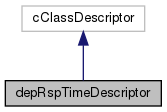
\includegraphics[width=197pt]{classdep_rsp_time_descriptor__inherit__graph}
\end{center}
\end{figure}


Collaboration diagram for dep\+Rsp\+Time\+Descriptor\+:\nopagebreak
\begin{figure}[H]
\begin{center}
\leavevmode
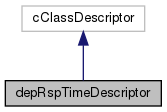
\includegraphics[width=197pt]{classdep_rsp_time_descriptor__coll__graph}
\end{center}
\end{figure}
\subsection*{Public Member Functions}
\begin{DoxyCompactItemize}
\item 
\hyperlink{classdep_rsp_time_descriptor_a1c9b594074be83beb7009019d66da91e}{dep\+Rsp\+Time\+Descriptor} ()
\item 
virtual \hyperlink{classdep_rsp_time_descriptor_a0cb36f001ae3e47a6d6156b8c7e66e19}{$\sim$dep\+Rsp\+Time\+Descriptor} ()
\item 
virtual bool \hyperlink{classdep_rsp_time_descriptor_ac514b2445c49b0a2fde22c730bdd8155}{does\+Support} (omnetpp\+::c\+Object $\ast$obj) const override
\item 
virtual const char $\ast$$\ast$ \hyperlink{classdep_rsp_time_descriptor_a3909adf8b159cd8da2cdb9aa135a77ba}{get\+Property\+Names} () const override
\item 
virtual const char $\ast$ \hyperlink{classdep_rsp_time_descriptor_a2426bb36989259be75b4ac3c7c18af5b}{get\+Property} (const char $\ast$propertyname) const override
\item 
virtual int \hyperlink{classdep_rsp_time_descriptor_ab44ba5e8986e63b20c2ced23f47a011c}{get\+Field\+Count} () const override
\item 
virtual const char $\ast$ \hyperlink{classdep_rsp_time_descriptor_a764ef69505cdeca4cefbda8aa3820bc3}{get\+Field\+Name} (int field) const override
\item 
virtual int \hyperlink{classdep_rsp_time_descriptor_aa50291bed26663e0840e5a9278af4145}{find\+Field} (const char $\ast$field\+Name) const override
\item 
virtual unsigned int \hyperlink{classdep_rsp_time_descriptor_aefc601d75b14b0e264693c32f35b084e}{get\+Field\+Type\+Flags} (int field) const override
\item 
virtual const char $\ast$ \hyperlink{classdep_rsp_time_descriptor_a230884891fa25dd60490fbf1b72dd5ab}{get\+Field\+Type\+String} (int field) const override
\item 
virtual const char $\ast$$\ast$ \hyperlink{classdep_rsp_time_descriptor_a35ad7064d9ca791511a1d570f957cb34}{get\+Field\+Property\+Names} (int field) const override
\item 
virtual const char $\ast$ \hyperlink{classdep_rsp_time_descriptor_a7c5adef7085e1e13c680e060fcdfd5a2}{get\+Field\+Property} (int field, const char $\ast$propertyname) const override
\item 
virtual int \hyperlink{classdep_rsp_time_descriptor_a1250376ef742580dc83db84ce3bc2283}{get\+Field\+Array\+Size} (void $\ast$object, int field) const override
\item 
virtual const char $\ast$ \hyperlink{classdep_rsp_time_descriptor_a792f2bfcb1f116dd06437d885ff72f48}{get\+Field\+Dynamic\+Type\+String} (void $\ast$object, int field, int i) const override
\item 
virtual std\+::string \hyperlink{classdep_rsp_time_descriptor_acdc1e2c5d57b9ade8cdd45472ca82719}{get\+Field\+Value\+As\+String} (void $\ast$object, int field, int i) const override
\item 
virtual bool \hyperlink{classdep_rsp_time_descriptor_a33a783027f6e9c827228f9405f485f63}{set\+Field\+Value\+As\+String} (void $\ast$object, int field, int i, const char $\ast$value) const override
\item 
virtual const char $\ast$ \hyperlink{classdep_rsp_time_descriptor_a55d83a6906074344459de31d49e51e1d}{get\+Field\+Struct\+Name} (int field) const override
\item 
virtual void $\ast$ \hyperlink{classdep_rsp_time_descriptor_ad6ca81a9ae888ced8f540d844900f30d}{get\+Field\+Struct\+Value\+Pointer} (void $\ast$object, int field, int i) const override
\end{DoxyCompactItemize}
\subsection*{Private Attributes}
\begin{DoxyCompactItemize}
\item 
const char $\ast$$\ast$ \hyperlink{classdep_rsp_time_descriptor_aa00fe09f472957d38fb825d538d5c090}{propertynames}
\end{DoxyCompactItemize}


\subsection{Constructor \& Destructor Documentation}
\mbox{\Hypertarget{classdep_rsp_time_descriptor_a1c9b594074be83beb7009019d66da91e}\label{classdep_rsp_time_descriptor_a1c9b594074be83beb7009019d66da91e}} 
\index{dep\+Rsp\+Time\+Descriptor@{dep\+Rsp\+Time\+Descriptor}!dep\+Rsp\+Time\+Descriptor@{dep\+Rsp\+Time\+Descriptor}}
\index{dep\+Rsp\+Time\+Descriptor@{dep\+Rsp\+Time\+Descriptor}!dep\+Rsp\+Time\+Descriptor@{dep\+Rsp\+Time\+Descriptor}}
\subsubsection{\texorpdfstring{dep\+Rsp\+Time\+Descriptor()}{depRspTimeDescriptor()}}
{\footnotesize\ttfamily dep\+Rsp\+Time\+Descriptor\+::dep\+Rsp\+Time\+Descriptor (\begin{DoxyParamCaption}{ }\end{DoxyParamCaption})}

\mbox{\Hypertarget{classdep_rsp_time_descriptor_a0cb36f001ae3e47a6d6156b8c7e66e19}\label{classdep_rsp_time_descriptor_a0cb36f001ae3e47a6d6156b8c7e66e19}} 
\index{dep\+Rsp\+Time\+Descriptor@{dep\+Rsp\+Time\+Descriptor}!````~dep\+Rsp\+Time\+Descriptor@{$\sim$dep\+Rsp\+Time\+Descriptor}}
\index{````~dep\+Rsp\+Time\+Descriptor@{$\sim$dep\+Rsp\+Time\+Descriptor}!dep\+Rsp\+Time\+Descriptor@{dep\+Rsp\+Time\+Descriptor}}
\subsubsection{\texorpdfstring{$\sim$dep\+Rsp\+Time\+Descriptor()}{~depRspTimeDescriptor()}}
{\footnotesize\ttfamily dep\+Rsp\+Time\+Descriptor\+::$\sim$dep\+Rsp\+Time\+Descriptor (\begin{DoxyParamCaption}{ }\end{DoxyParamCaption})\hspace{0.3cm}{\ttfamily [virtual]}}



\subsection{Member Function Documentation}
\mbox{\Hypertarget{classdep_rsp_time_descriptor_ac514b2445c49b0a2fde22c730bdd8155}\label{classdep_rsp_time_descriptor_ac514b2445c49b0a2fde22c730bdd8155}} 
\index{dep\+Rsp\+Time\+Descriptor@{dep\+Rsp\+Time\+Descriptor}!does\+Support@{does\+Support}}
\index{does\+Support@{does\+Support}!dep\+Rsp\+Time\+Descriptor@{dep\+Rsp\+Time\+Descriptor}}
\subsubsection{\texorpdfstring{does\+Support()}{doesSupport()}}
{\footnotesize\ttfamily bool dep\+Rsp\+Time\+Descriptor\+::does\+Support (\begin{DoxyParamCaption}\item[{omnetpp\+::c\+Object $\ast$}]{obj }\end{DoxyParamCaption}) const\hspace{0.3cm}{\ttfamily [override]}, {\ttfamily [virtual]}}

\mbox{\Hypertarget{classdep_rsp_time_descriptor_aa50291bed26663e0840e5a9278af4145}\label{classdep_rsp_time_descriptor_aa50291bed26663e0840e5a9278af4145}} 
\index{dep\+Rsp\+Time\+Descriptor@{dep\+Rsp\+Time\+Descriptor}!find\+Field@{find\+Field}}
\index{find\+Field@{find\+Field}!dep\+Rsp\+Time\+Descriptor@{dep\+Rsp\+Time\+Descriptor}}
\subsubsection{\texorpdfstring{find\+Field()}{findField()}}
{\footnotesize\ttfamily int dep\+Rsp\+Time\+Descriptor\+::find\+Field (\begin{DoxyParamCaption}\item[{const char $\ast$}]{field\+Name }\end{DoxyParamCaption}) const\hspace{0.3cm}{\ttfamily [override]}, {\ttfamily [virtual]}}

\mbox{\Hypertarget{classdep_rsp_time_descriptor_a1250376ef742580dc83db84ce3bc2283}\label{classdep_rsp_time_descriptor_a1250376ef742580dc83db84ce3bc2283}} 
\index{dep\+Rsp\+Time\+Descriptor@{dep\+Rsp\+Time\+Descriptor}!get\+Field\+Array\+Size@{get\+Field\+Array\+Size}}
\index{get\+Field\+Array\+Size@{get\+Field\+Array\+Size}!dep\+Rsp\+Time\+Descriptor@{dep\+Rsp\+Time\+Descriptor}}
\subsubsection{\texorpdfstring{get\+Field\+Array\+Size()}{getFieldArraySize()}}
{\footnotesize\ttfamily int dep\+Rsp\+Time\+Descriptor\+::get\+Field\+Array\+Size (\begin{DoxyParamCaption}\item[{void $\ast$}]{object,  }\item[{int}]{field }\end{DoxyParamCaption}) const\hspace{0.3cm}{\ttfamily [override]}, {\ttfamily [virtual]}}

\mbox{\Hypertarget{classdep_rsp_time_descriptor_ab44ba5e8986e63b20c2ced23f47a011c}\label{classdep_rsp_time_descriptor_ab44ba5e8986e63b20c2ced23f47a011c}} 
\index{dep\+Rsp\+Time\+Descriptor@{dep\+Rsp\+Time\+Descriptor}!get\+Field\+Count@{get\+Field\+Count}}
\index{get\+Field\+Count@{get\+Field\+Count}!dep\+Rsp\+Time\+Descriptor@{dep\+Rsp\+Time\+Descriptor}}
\subsubsection{\texorpdfstring{get\+Field\+Count()}{getFieldCount()}}
{\footnotesize\ttfamily int dep\+Rsp\+Time\+Descriptor\+::get\+Field\+Count (\begin{DoxyParamCaption}{ }\end{DoxyParamCaption}) const\hspace{0.3cm}{\ttfamily [override]}, {\ttfamily [virtual]}}

\mbox{\Hypertarget{classdep_rsp_time_descriptor_a792f2bfcb1f116dd06437d885ff72f48}\label{classdep_rsp_time_descriptor_a792f2bfcb1f116dd06437d885ff72f48}} 
\index{dep\+Rsp\+Time\+Descriptor@{dep\+Rsp\+Time\+Descriptor}!get\+Field\+Dynamic\+Type\+String@{get\+Field\+Dynamic\+Type\+String}}
\index{get\+Field\+Dynamic\+Type\+String@{get\+Field\+Dynamic\+Type\+String}!dep\+Rsp\+Time\+Descriptor@{dep\+Rsp\+Time\+Descriptor}}
\subsubsection{\texorpdfstring{get\+Field\+Dynamic\+Type\+String()}{getFieldDynamicTypeString()}}
{\footnotesize\ttfamily const char $\ast$ dep\+Rsp\+Time\+Descriptor\+::get\+Field\+Dynamic\+Type\+String (\begin{DoxyParamCaption}\item[{void $\ast$}]{object,  }\item[{int}]{field,  }\item[{int}]{i }\end{DoxyParamCaption}) const\hspace{0.3cm}{\ttfamily [override]}, {\ttfamily [virtual]}}

\mbox{\Hypertarget{classdep_rsp_time_descriptor_a764ef69505cdeca4cefbda8aa3820bc3}\label{classdep_rsp_time_descriptor_a764ef69505cdeca4cefbda8aa3820bc3}} 
\index{dep\+Rsp\+Time\+Descriptor@{dep\+Rsp\+Time\+Descriptor}!get\+Field\+Name@{get\+Field\+Name}}
\index{get\+Field\+Name@{get\+Field\+Name}!dep\+Rsp\+Time\+Descriptor@{dep\+Rsp\+Time\+Descriptor}}
\subsubsection{\texorpdfstring{get\+Field\+Name()}{getFieldName()}}
{\footnotesize\ttfamily const char $\ast$ dep\+Rsp\+Time\+Descriptor\+::get\+Field\+Name (\begin{DoxyParamCaption}\item[{int}]{field }\end{DoxyParamCaption}) const\hspace{0.3cm}{\ttfamily [override]}, {\ttfamily [virtual]}}

\mbox{\Hypertarget{classdep_rsp_time_descriptor_a7c5adef7085e1e13c680e060fcdfd5a2}\label{classdep_rsp_time_descriptor_a7c5adef7085e1e13c680e060fcdfd5a2}} 
\index{dep\+Rsp\+Time\+Descriptor@{dep\+Rsp\+Time\+Descriptor}!get\+Field\+Property@{get\+Field\+Property}}
\index{get\+Field\+Property@{get\+Field\+Property}!dep\+Rsp\+Time\+Descriptor@{dep\+Rsp\+Time\+Descriptor}}
\subsubsection{\texorpdfstring{get\+Field\+Property()}{getFieldProperty()}}
{\footnotesize\ttfamily const char $\ast$ dep\+Rsp\+Time\+Descriptor\+::get\+Field\+Property (\begin{DoxyParamCaption}\item[{int}]{field,  }\item[{const char $\ast$}]{propertyname }\end{DoxyParamCaption}) const\hspace{0.3cm}{\ttfamily [override]}, {\ttfamily [virtual]}}

\mbox{\Hypertarget{classdep_rsp_time_descriptor_a35ad7064d9ca791511a1d570f957cb34}\label{classdep_rsp_time_descriptor_a35ad7064d9ca791511a1d570f957cb34}} 
\index{dep\+Rsp\+Time\+Descriptor@{dep\+Rsp\+Time\+Descriptor}!get\+Field\+Property\+Names@{get\+Field\+Property\+Names}}
\index{get\+Field\+Property\+Names@{get\+Field\+Property\+Names}!dep\+Rsp\+Time\+Descriptor@{dep\+Rsp\+Time\+Descriptor}}
\subsubsection{\texorpdfstring{get\+Field\+Property\+Names()}{getFieldPropertyNames()}}
{\footnotesize\ttfamily const char $\ast$$\ast$ dep\+Rsp\+Time\+Descriptor\+::get\+Field\+Property\+Names (\begin{DoxyParamCaption}\item[{int}]{field }\end{DoxyParamCaption}) const\hspace{0.3cm}{\ttfamily [override]}, {\ttfamily [virtual]}}

\mbox{\Hypertarget{classdep_rsp_time_descriptor_a55d83a6906074344459de31d49e51e1d}\label{classdep_rsp_time_descriptor_a55d83a6906074344459de31d49e51e1d}} 
\index{dep\+Rsp\+Time\+Descriptor@{dep\+Rsp\+Time\+Descriptor}!get\+Field\+Struct\+Name@{get\+Field\+Struct\+Name}}
\index{get\+Field\+Struct\+Name@{get\+Field\+Struct\+Name}!dep\+Rsp\+Time\+Descriptor@{dep\+Rsp\+Time\+Descriptor}}
\subsubsection{\texorpdfstring{get\+Field\+Struct\+Name()}{getFieldStructName()}}
{\footnotesize\ttfamily const char $\ast$ dep\+Rsp\+Time\+Descriptor\+::get\+Field\+Struct\+Name (\begin{DoxyParamCaption}\item[{int}]{field }\end{DoxyParamCaption}) const\hspace{0.3cm}{\ttfamily [override]}, {\ttfamily [virtual]}}

\mbox{\Hypertarget{classdep_rsp_time_descriptor_ad6ca81a9ae888ced8f540d844900f30d}\label{classdep_rsp_time_descriptor_ad6ca81a9ae888ced8f540d844900f30d}} 
\index{dep\+Rsp\+Time\+Descriptor@{dep\+Rsp\+Time\+Descriptor}!get\+Field\+Struct\+Value\+Pointer@{get\+Field\+Struct\+Value\+Pointer}}
\index{get\+Field\+Struct\+Value\+Pointer@{get\+Field\+Struct\+Value\+Pointer}!dep\+Rsp\+Time\+Descriptor@{dep\+Rsp\+Time\+Descriptor}}
\subsubsection{\texorpdfstring{get\+Field\+Struct\+Value\+Pointer()}{getFieldStructValuePointer()}}
{\footnotesize\ttfamily void $\ast$ dep\+Rsp\+Time\+Descriptor\+::get\+Field\+Struct\+Value\+Pointer (\begin{DoxyParamCaption}\item[{void $\ast$}]{object,  }\item[{int}]{field,  }\item[{int}]{i }\end{DoxyParamCaption}) const\hspace{0.3cm}{\ttfamily [override]}, {\ttfamily [virtual]}}

\mbox{\Hypertarget{classdep_rsp_time_descriptor_aefc601d75b14b0e264693c32f35b084e}\label{classdep_rsp_time_descriptor_aefc601d75b14b0e264693c32f35b084e}} 
\index{dep\+Rsp\+Time\+Descriptor@{dep\+Rsp\+Time\+Descriptor}!get\+Field\+Type\+Flags@{get\+Field\+Type\+Flags}}
\index{get\+Field\+Type\+Flags@{get\+Field\+Type\+Flags}!dep\+Rsp\+Time\+Descriptor@{dep\+Rsp\+Time\+Descriptor}}
\subsubsection{\texorpdfstring{get\+Field\+Type\+Flags()}{getFieldTypeFlags()}}
{\footnotesize\ttfamily unsigned int dep\+Rsp\+Time\+Descriptor\+::get\+Field\+Type\+Flags (\begin{DoxyParamCaption}\item[{int}]{field }\end{DoxyParamCaption}) const\hspace{0.3cm}{\ttfamily [override]}, {\ttfamily [virtual]}}

\mbox{\Hypertarget{classdep_rsp_time_descriptor_a230884891fa25dd60490fbf1b72dd5ab}\label{classdep_rsp_time_descriptor_a230884891fa25dd60490fbf1b72dd5ab}} 
\index{dep\+Rsp\+Time\+Descriptor@{dep\+Rsp\+Time\+Descriptor}!get\+Field\+Type\+String@{get\+Field\+Type\+String}}
\index{get\+Field\+Type\+String@{get\+Field\+Type\+String}!dep\+Rsp\+Time\+Descriptor@{dep\+Rsp\+Time\+Descriptor}}
\subsubsection{\texorpdfstring{get\+Field\+Type\+String()}{getFieldTypeString()}}
{\footnotesize\ttfamily const char $\ast$ dep\+Rsp\+Time\+Descriptor\+::get\+Field\+Type\+String (\begin{DoxyParamCaption}\item[{int}]{field }\end{DoxyParamCaption}) const\hspace{0.3cm}{\ttfamily [override]}, {\ttfamily [virtual]}}

\mbox{\Hypertarget{classdep_rsp_time_descriptor_acdc1e2c5d57b9ade8cdd45472ca82719}\label{classdep_rsp_time_descriptor_acdc1e2c5d57b9ade8cdd45472ca82719}} 
\index{dep\+Rsp\+Time\+Descriptor@{dep\+Rsp\+Time\+Descriptor}!get\+Field\+Value\+As\+String@{get\+Field\+Value\+As\+String}}
\index{get\+Field\+Value\+As\+String@{get\+Field\+Value\+As\+String}!dep\+Rsp\+Time\+Descriptor@{dep\+Rsp\+Time\+Descriptor}}
\subsubsection{\texorpdfstring{get\+Field\+Value\+As\+String()}{getFieldValueAsString()}}
{\footnotesize\ttfamily std\+::string dep\+Rsp\+Time\+Descriptor\+::get\+Field\+Value\+As\+String (\begin{DoxyParamCaption}\item[{void $\ast$}]{object,  }\item[{int}]{field,  }\item[{int}]{i }\end{DoxyParamCaption}) const\hspace{0.3cm}{\ttfamily [override]}, {\ttfamily [virtual]}}

\mbox{\Hypertarget{classdep_rsp_time_descriptor_a2426bb36989259be75b4ac3c7c18af5b}\label{classdep_rsp_time_descriptor_a2426bb36989259be75b4ac3c7c18af5b}} 
\index{dep\+Rsp\+Time\+Descriptor@{dep\+Rsp\+Time\+Descriptor}!get\+Property@{get\+Property}}
\index{get\+Property@{get\+Property}!dep\+Rsp\+Time\+Descriptor@{dep\+Rsp\+Time\+Descriptor}}
\subsubsection{\texorpdfstring{get\+Property()}{getProperty()}}
{\footnotesize\ttfamily const char $\ast$ dep\+Rsp\+Time\+Descriptor\+::get\+Property (\begin{DoxyParamCaption}\item[{const char $\ast$}]{propertyname }\end{DoxyParamCaption}) const\hspace{0.3cm}{\ttfamily [override]}, {\ttfamily [virtual]}}

\mbox{\Hypertarget{classdep_rsp_time_descriptor_a3909adf8b159cd8da2cdb9aa135a77ba}\label{classdep_rsp_time_descriptor_a3909adf8b159cd8da2cdb9aa135a77ba}} 
\index{dep\+Rsp\+Time\+Descriptor@{dep\+Rsp\+Time\+Descriptor}!get\+Property\+Names@{get\+Property\+Names}}
\index{get\+Property\+Names@{get\+Property\+Names}!dep\+Rsp\+Time\+Descriptor@{dep\+Rsp\+Time\+Descriptor}}
\subsubsection{\texorpdfstring{get\+Property\+Names()}{getPropertyNames()}}
{\footnotesize\ttfamily const char $\ast$$\ast$ dep\+Rsp\+Time\+Descriptor\+::get\+Property\+Names (\begin{DoxyParamCaption}{ }\end{DoxyParamCaption}) const\hspace{0.3cm}{\ttfamily [override]}, {\ttfamily [virtual]}}

\mbox{\Hypertarget{classdep_rsp_time_descriptor_a33a783027f6e9c827228f9405f485f63}\label{classdep_rsp_time_descriptor_a33a783027f6e9c827228f9405f485f63}} 
\index{dep\+Rsp\+Time\+Descriptor@{dep\+Rsp\+Time\+Descriptor}!set\+Field\+Value\+As\+String@{set\+Field\+Value\+As\+String}}
\index{set\+Field\+Value\+As\+String@{set\+Field\+Value\+As\+String}!dep\+Rsp\+Time\+Descriptor@{dep\+Rsp\+Time\+Descriptor}}
\subsubsection{\texorpdfstring{set\+Field\+Value\+As\+String()}{setFieldValueAsString()}}
{\footnotesize\ttfamily bool dep\+Rsp\+Time\+Descriptor\+::set\+Field\+Value\+As\+String (\begin{DoxyParamCaption}\item[{void $\ast$}]{object,  }\item[{int}]{field,  }\item[{int}]{i,  }\item[{const char $\ast$}]{value }\end{DoxyParamCaption}) const\hspace{0.3cm}{\ttfamily [override]}, {\ttfamily [virtual]}}



\subsection{Member Data Documentation}
\mbox{\Hypertarget{classdep_rsp_time_descriptor_aa00fe09f472957d38fb825d538d5c090}\label{classdep_rsp_time_descriptor_aa00fe09f472957d38fb825d538d5c090}} 
\index{dep\+Rsp\+Time\+Descriptor@{dep\+Rsp\+Time\+Descriptor}!propertynames@{propertynames}}
\index{propertynames@{propertynames}!dep\+Rsp\+Time\+Descriptor@{dep\+Rsp\+Time\+Descriptor}}
\subsubsection{\texorpdfstring{propertynames}{propertynames}}
{\footnotesize\ttfamily const char$\ast$$\ast$ dep\+Rsp\+Time\+Descriptor\+::propertynames\hspace{0.3cm}{\ttfamily [mutable]}, {\ttfamily [private]}}



The documentation for this class was generated from the following file\+:\begin{DoxyCompactItemize}
\item 
src/\+Messages/\hyperlink{dep_rsp__m_8cc}{dep\+Rsp\+\_\+m.\+cc}\end{DoxyCompactItemize}

\hypertarget{class_error_detector}{}\section{Error\+Detector Class Reference}
\label{class_error_detector}\index{Error\+Detector@{Error\+Detector}}


Base class of error detectors.  




{\ttfamily \#include $<$Error\+Detector.\+h$>$}



Inheritance diagram for Error\+Detector\+:\nopagebreak
\begin{figure}[H]
\begin{center}
\leavevmode
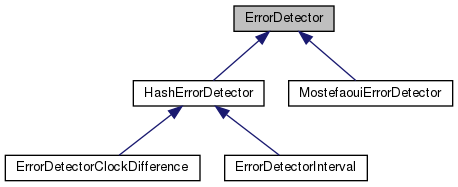
\includegraphics[width=350pt]{class_error_detector__inherit__graph}
\end{center}
\end{figure}


Collaboration diagram for Error\+Detector\+:\nopagebreak
\begin{figure}[H]
\begin{center}
\leavevmode
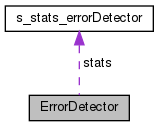
\includegraphics[width=191pt]{class_error_detector__coll__graph}
\end{center}
\end{figure}
\subsection*{Public Member Functions}
\begin{DoxyCompactItemize}
\item 
\hyperlink{class_error_detector_ae851a02dff242968cd6419400271d74f}{Error\+Detector} ()
\item 
virtual \hyperlink{class_error_detector_a3708d713f8f7bee01aa7e5a2fb7bb652}{$\sim$\+Error\+Detector} ()=0
\item 
virtual \hyperlink{class_app_msg}{App\+Msg} $\ast$ \hyperlink{class_error_detector_a8cac1f6ac6803da4379df7891789c490}{prepare\+Message} (\hyperlink{class_app_msg}{App\+Msg} $\ast$m, const vector$<$ \hyperlink{structures_8h_a7e7bdc1d2fff8a9436f2f352b2711ed6}{message\+Info} $>$ \&delivered, const \hyperlink{class_probabilistic_clock}{Probabilistic\+Clock} \&clock, const \hyperlink{class_total_dependencies}{Total\+Dependencies} \&process\+Dependencies)=0
\begin{DoxyCompactList}\small\item\em Appends to the message to broadcast the information the destination error detector requires. \end{DoxyCompactList}\item 
virtual bool \hyperlink{class_error_detector_afc717d04768dd207196c08e24163115c}{test} (\hyperlink{structures_8h_a7e7bdc1d2fff8a9436f2f352b2711ed6}{message\+Info} message, const vector$<$ unsigned int $>$ \&incremented\+Clock\+Entries, const \hyperlink{class_probabilistic_clock}{Probabilistic\+Clock} \&process\+Clock, const \hyperlink{class_total_dependencies}{Total\+Dependencies} \&process\+Dependencies, \hyperlink{class_controller}{Controller} $\ast$control, \hyperlink{class_simulation_parameters}{Simulation\+Parameters} $\ast$params, const vector$<$ \hyperlink{structures_8h_a7e7bdc1d2fff8a9436f2f352b2711ed6}{message\+Info} $>$ \&delivered)=0
\begin{DoxyCompactList}\small\item\em Error detector test to determine if the message to deliver can be delivered in causal order. \end{DoxyCompactList}\end{DoxyCompactItemize}
\subsection*{Private Attributes}
\begin{DoxyCompactItemize}
\item 
\hyperlink{_error_detector_8h_abbc922e22c7b55f0bd58bea618eec587}{stats\+\_\+error\+Detector} \hyperlink{class_error_detector_acb550f19c1da2d61d40757351f96d4b1}{stats}
\end{DoxyCompactItemize}
\subsection*{Friends}
\begin{DoxyCompactItemize}
\item 
class \hyperlink{class_error_detector_a129f65b6976377739eb6231b6962985e}{Stats}
\item 
class \hyperlink{class_error_detector_aa0495b79e94b09962892b921ae370e57}{Node\+Without\+Recovery}
\item 
class \hyperlink{class_error_detector_af62fbc8632478613aa92b0e55c79510e}{Node\+With\+Recovery}
\item 
class \hyperlink{class_error_detector_a4a759c82473f06c7e89c3d75a509a390}{Node\+With\+Recovery\+Test}
\end{DoxyCompactItemize}


\subsection{Detailed Description}
Base class of error detectors. 

\subsection{Constructor \& Destructor Documentation}
\mbox{\Hypertarget{class_error_detector_ae851a02dff242968cd6419400271d74f}\label{class_error_detector_ae851a02dff242968cd6419400271d74f}} 
\index{Error\+Detector@{Error\+Detector}!Error\+Detector@{Error\+Detector}}
\index{Error\+Detector@{Error\+Detector}!Error\+Detector@{Error\+Detector}}
\subsubsection{\texorpdfstring{Error\+Detector()}{ErrorDetector()}}
{\footnotesize\ttfamily Error\+Detector\+::\+Error\+Detector (\begin{DoxyParamCaption}{ }\end{DoxyParamCaption})}

\mbox{\Hypertarget{class_error_detector_a3708d713f8f7bee01aa7e5a2fb7bb652}\label{class_error_detector_a3708d713f8f7bee01aa7e5a2fb7bb652}} 
\index{Error\+Detector@{Error\+Detector}!````~Error\+Detector@{$\sim$\+Error\+Detector}}
\index{````~Error\+Detector@{$\sim$\+Error\+Detector}!Error\+Detector@{Error\+Detector}}
\subsubsection{\texorpdfstring{$\sim$\+Error\+Detector()}{~ErrorDetector()}}
{\footnotesize\ttfamily Error\+Detector\+::$\sim$\+Error\+Detector (\begin{DoxyParamCaption}{ }\end{DoxyParamCaption})\hspace{0.3cm}{\ttfamily [pure virtual]}, {\ttfamily [default]}}



\subsection{Member Function Documentation}
\mbox{\Hypertarget{class_error_detector_a8cac1f6ac6803da4379df7891789c490}\label{class_error_detector_a8cac1f6ac6803da4379df7891789c490}} 
\index{Error\+Detector@{Error\+Detector}!prepare\+Message@{prepare\+Message}}
\index{prepare\+Message@{prepare\+Message}!Error\+Detector@{Error\+Detector}}
\subsubsection{\texorpdfstring{prepare\+Message()}{prepareMessage()}}
{\footnotesize\ttfamily virtual \hyperlink{class_app_msg}{App\+Msg}$\ast$ Error\+Detector\+::prepare\+Message (\begin{DoxyParamCaption}\item[{\hyperlink{class_app_msg}{App\+Msg} $\ast$}]{m,  }\item[{const vector$<$ \hyperlink{structures_8h_a7e7bdc1d2fff8a9436f2f352b2711ed6}{message\+Info} $>$ \&}]{delivered,  }\item[{const \hyperlink{class_probabilistic_clock}{Probabilistic\+Clock} \&}]{clock,  }\item[{const \hyperlink{class_total_dependencies}{Total\+Dependencies} \&}]{process\+Dependencies }\end{DoxyParamCaption})\hspace{0.3cm}{\ttfamily [pure virtual]}}



Appends to the message to broadcast the information the destination error detector requires. 



Implemented in \hyperlink{class_hash_error_detector_a2b1dad6a83a08fd7ce88e32f84638459}{Hash\+Error\+Detector}, and \hyperlink{class_mostefaoui_error_detector_adcd530d7349df19adb614ca414225214}{Mostefaoui\+Error\+Detector}.

\mbox{\Hypertarget{class_error_detector_afc717d04768dd207196c08e24163115c}\label{class_error_detector_afc717d04768dd207196c08e24163115c}} 
\index{Error\+Detector@{Error\+Detector}!test@{test}}
\index{test@{test}!Error\+Detector@{Error\+Detector}}
\subsubsection{\texorpdfstring{test()}{test()}}
{\footnotesize\ttfamily virtual bool Error\+Detector\+::test (\begin{DoxyParamCaption}\item[{\hyperlink{structures_8h_a7e7bdc1d2fff8a9436f2f352b2711ed6}{message\+Info}}]{message,  }\item[{const vector$<$ unsigned int $>$ \&}]{incremented\+Clock\+Entries,  }\item[{const \hyperlink{class_probabilistic_clock}{Probabilistic\+Clock} \&}]{process\+Clock,  }\item[{const \hyperlink{class_total_dependencies}{Total\+Dependencies} \&}]{process\+Dependencies,  }\item[{\hyperlink{class_controller}{Controller} $\ast$}]{control,  }\item[{\hyperlink{class_simulation_parameters}{Simulation\+Parameters} $\ast$}]{params,  }\item[{const vector$<$ \hyperlink{structures_8h_a7e7bdc1d2fff8a9436f2f352b2711ed6}{message\+Info} $>$ \&}]{delivered }\end{DoxyParamCaption})\hspace{0.3cm}{\ttfamily [pure virtual]}}



Error detector test to determine if the message to deliver can be delivered in causal order. 



Implemented in \hyperlink{class_hash_error_detector_a1c7fe649a34cf7e139ce53a248dce748}{Hash\+Error\+Detector}, and \hyperlink{class_mostefaoui_error_detector_a293f6cf144526bc8694fc4f1fc0daeb5}{Mostefaoui\+Error\+Detector}.



\subsection{Friends And Related Function Documentation}
\mbox{\Hypertarget{class_error_detector_aa0495b79e94b09962892b921ae370e57}\label{class_error_detector_aa0495b79e94b09962892b921ae370e57}} 
\index{Error\+Detector@{Error\+Detector}!Node\+Without\+Recovery@{Node\+Without\+Recovery}}
\index{Node\+Without\+Recovery@{Node\+Without\+Recovery}!Error\+Detector@{Error\+Detector}}
\subsubsection{\texorpdfstring{Node\+Without\+Recovery}{NodeWithoutRecovery}}
{\footnotesize\ttfamily friend class \hyperlink{class_node_without_recovery}{Node\+Without\+Recovery}\hspace{0.3cm}{\ttfamily [friend]}}

\mbox{\Hypertarget{class_error_detector_af62fbc8632478613aa92b0e55c79510e}\label{class_error_detector_af62fbc8632478613aa92b0e55c79510e}} 
\index{Error\+Detector@{Error\+Detector}!Node\+With\+Recovery@{Node\+With\+Recovery}}
\index{Node\+With\+Recovery@{Node\+With\+Recovery}!Error\+Detector@{Error\+Detector}}
\subsubsection{\texorpdfstring{Node\+With\+Recovery}{NodeWithRecovery}}
{\footnotesize\ttfamily friend class \hyperlink{class_node_with_recovery}{Node\+With\+Recovery}\hspace{0.3cm}{\ttfamily [friend]}}

\mbox{\Hypertarget{class_error_detector_a4a759c82473f06c7e89c3d75a509a390}\label{class_error_detector_a4a759c82473f06c7e89c3d75a509a390}} 
\index{Error\+Detector@{Error\+Detector}!Node\+With\+Recovery\+Test@{Node\+With\+Recovery\+Test}}
\index{Node\+With\+Recovery\+Test@{Node\+With\+Recovery\+Test}!Error\+Detector@{Error\+Detector}}
\subsubsection{\texorpdfstring{Node\+With\+Recovery\+Test}{NodeWithRecoveryTest}}
{\footnotesize\ttfamily friend class \hyperlink{class_node_with_recovery_test}{Node\+With\+Recovery\+Test}\hspace{0.3cm}{\ttfamily [friend]}}

\mbox{\Hypertarget{class_error_detector_a129f65b6976377739eb6231b6962985e}\label{class_error_detector_a129f65b6976377739eb6231b6962985e}} 
\index{Error\+Detector@{Error\+Detector}!Stats@{Stats}}
\index{Stats@{Stats}!Error\+Detector@{Error\+Detector}}
\subsubsection{\texorpdfstring{Stats}{Stats}}
{\footnotesize\ttfamily friend class \hyperlink{class_stats}{Stats}\hspace{0.3cm}{\ttfamily [friend]}}



\subsection{Member Data Documentation}
\mbox{\Hypertarget{class_error_detector_acb550f19c1da2d61d40757351f96d4b1}\label{class_error_detector_acb550f19c1da2d61d40757351f96d4b1}} 
\index{Error\+Detector@{Error\+Detector}!stats@{stats}}
\index{stats@{stats}!Error\+Detector@{Error\+Detector}}
\subsubsection{\texorpdfstring{stats}{stats}}
{\footnotesize\ttfamily \hyperlink{_error_detector_8h_abbc922e22c7b55f0bd58bea618eec587}{stats\+\_\+error\+Detector} Error\+Detector\+::stats\hspace{0.3cm}{\ttfamily [private]}}



The documentation for this class was generated from the following files\+:\begin{DoxyCompactItemize}
\item 
src/\+Detectors/\hyperlink{_error_detector_8h}{Error\+Detector.\+h}\item 
src/\+Detectors/\hyperlink{_error_detector_8cc}{Error\+Detector.\+cc}\end{DoxyCompactItemize}

\hypertarget{class_error_detector_clock_difference}{}\section{Error\+Detector\+Clock\+Difference Class Reference}
\label{class_error_detector_clock_difference}\index{Error\+Detector\+Clock\+Difference@{Error\+Detector\+Clock\+Difference}}


Hash-\/based error detector that uses the clock difference between message to determine the causal dependencies of messages.  




{\ttfamily \#include $<$Hash\+Error\+Detector\+Clock\+Difference.\+h$>$}



Inheritance diagram for Error\+Detector\+Clock\+Difference\+:
\nopagebreak
\begin{figure}[H]
\begin{center}
\leavevmode
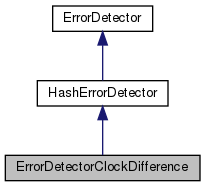
\includegraphics[width=226pt]{class_error_detector_clock_difference__inherit__graph}
\end{center}
\end{figure}


Collaboration diagram for Error\+Detector\+Clock\+Difference\+:
\nopagebreak
\begin{figure}[H]
\begin{center}
\leavevmode
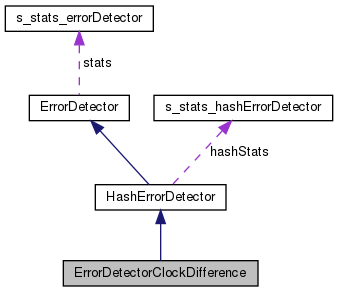
\includegraphics[width=326pt]{class_error_detector_clock_difference__coll__graph}
\end{center}
\end{figure}
\subsection*{Public Member Functions}
\begin{DoxyCompactItemize}
\item 
\hyperlink{class_error_detector_clock_difference_a5edb355be9179cd604d3e7f946846c55}{Error\+Detector\+Clock\+Difference} ()
\item 
virtual \hyperlink{class_error_detector_clock_difference_a19bda307bcb9a8974a97fdf56fb77b8f}{$\sim$\+Error\+Detector\+Clock\+Difference} ()
\item 
virtual vector$<$ \hyperlink{structures_8h_a83a1d9a070efa5341da84cfd8e28d3e5}{id\+Msg} $>$ \hyperlink{class_error_detector_clock_difference_a15406c8d7652f3b9358b1958d3723933}{determine\+And\+Get\+Appended\+Dependencies} (const vector$<$ \hyperlink{structures_8h_a7e7bdc1d2fff8a9436f2f352b2711ed6}{message\+Info} $>$ \&delivered, const \hyperlink{class_probabilistic_clock}{Probabilistic\+Clock} \&clock)
\begin{DoxyCompactList}\small\item\em Determines the causal dependencies to append on the message to broadcast. \end{DoxyCompactList}\item 
bool \hyperlink{class_error_detector_clock_difference_a4d399849b1872d3273fa757ee9dc9bd9}{is\+Considered\+As\+Dependency} (const \hyperlink{structures_8h_a7e7bdc1d2fff8a9436f2f352b2711ed6}{message\+Info} \&message, const \hyperlink{structures_8h_a7e7bdc1d2fff8a9436f2f352b2711ed6}{message\+Info} \&possible\+Dep)
\begin{DoxyCompactList}\small\item\em Determines if a message is considered as being a dependency. \end{DoxyCompactList}\item 
bool \hyperlink{class_error_detector_clock_difference_ab20aa1671eb558dea6f06b2440e97e41}{is\+Considered\+As\+Possible\+Dependency} (const \hyperlink{structures_8h_a7e7bdc1d2fff8a9436f2f352b2711ed6}{message\+Info} \&message, const \hyperlink{structures_8h_a7e7bdc1d2fff8a9436f2f352b2711ed6}{message\+Info} \&possible\+Dep)
\begin{DoxyCompactList}\small\item\em Determines if a message is considered as being a possible dependency. \end{DoxyCompactList}\item 
vector$<$ \hyperlink{structures_8h_a83a1d9a070efa5341da84cfd8e28d3e5}{id\+Msg} $>$ \hyperlink{class_error_detector_clock_difference_a6dafc330591db83f5c5fbee56b2c4937}{sort\+Possible\+Dependencies\+Set} (const \hyperlink{structures_8h_a7e7bdc1d2fff8a9436f2f352b2711ed6}{message\+Info} \&message, const vector$<$ \hyperlink{structures_8h_a7e7bdc1d2fff8a9436f2f352b2711ed6}{message\+Info} $>$ \&base\+Combine\+Set)
\begin{DoxyCompactList}\small\item\em Sorts the set of possible dependencies depending on the clock difference of messages with the message to broadcast. \end{DoxyCompactList}\item 
void \hyperlink{class_error_detector_clock_difference_a529b87b6eaee9041601af1ca36b51c93}{set\+Clock\+Difference\+Considered\+Dependency} (unsigned int message\+Load, unsigned nb\+Incremented\+Entries)
\begin{DoxyCompactList}\small\item\em Sets the clock difference over which a message is considered as having been delivered by all nodes and is therefore considered as being a causal dependency of the message to deliver. \end{DoxyCompactList}\item 
\hyperlink{class_partial_dependencies}{Partial\+Dependencies} \hyperlink{class_error_detector_clock_difference_a26f4c2905859947201d0a18146f2e961}{get\+Partial\+Dependencies} (const vector$<$ \hyperlink{structures_8h_a7e7bdc1d2fff8a9436f2f352b2711ed6}{message\+Info} $>$ \&delivered, const \hyperlink{class_probabilistic_clock}{Probabilistic\+Clock} \&clock)
\begin{DoxyCompactList}\small\item\em Get partial dependencies of the message to broadcast. \end{DoxyCompactList}\end{DoxyCompactItemize}
\subsection*{Private Attributes}
\begin{DoxyCompactItemize}
\item 
unsigned int \hyperlink{class_error_detector_clock_difference_a0d2a3c4111e8bb4b3c232aacca9a0062}{clock\+Difference\+Considered\+Dependency} = 100
\begin{DoxyCompactList}\small\item\em The clock difference over which a message is considered as having been delivered by all nodes and is thus not taken into account in the hash computation. \end{DoxyCompactList}\item 
unsigned int \hyperlink{class_error_detector_clock_difference_aa733fc7d2023d62a7418ca20e01e9f5a}{clock\+Difference\+Considered\+Not\+Dependency} = 0
\begin{DoxyCompactList}\small\item\em The clock difference under which a message is considered as not being a dependency of a message to deliver, because its low clock difference indicates that it has been broadcasted in a time interval very clock to the broadcast of the message to deliver. \end{DoxyCompactList}\end{DoxyCompactItemize}


\subsection{Detailed Description}
Hash-\/based error detector that uses the clock difference between message to determine the causal dependencies of messages. 

Assumes that probabilistic clocks increase over time. Thus, the greater the clock difference between two messages, the greater the duration between their broadcast. Therefore, messages over a given clock difference are considered as having been delivered by all nodes, and are not considered in the hash computation. 

\subsection{Constructor \& Destructor Documentation}
\mbox{\Hypertarget{class_error_detector_clock_difference_a5edb355be9179cd604d3e7f946846c55}\label{class_error_detector_clock_difference_a5edb355be9179cd604d3e7f946846c55}} 
\index{Error\+Detector\+Clock\+Difference@{Error\+Detector\+Clock\+Difference}!Error\+Detector\+Clock\+Difference@{Error\+Detector\+Clock\+Difference}}
\index{Error\+Detector\+Clock\+Difference@{Error\+Detector\+Clock\+Difference}!Error\+Detector\+Clock\+Difference@{Error\+Detector\+Clock\+Difference}}
\subsubsection{\texorpdfstring{Error\+Detector\+Clock\+Difference()}{ErrorDetectorClockDifference()}}
{\footnotesize\ttfamily Error\+Detector\+Clock\+Difference\+::\+Error\+Detector\+Clock\+Difference (\begin{DoxyParamCaption}{ }\end{DoxyParamCaption})}

\mbox{\Hypertarget{class_error_detector_clock_difference_a19bda307bcb9a8974a97fdf56fb77b8f}\label{class_error_detector_clock_difference_a19bda307bcb9a8974a97fdf56fb77b8f}} 
\index{Error\+Detector\+Clock\+Difference@{Error\+Detector\+Clock\+Difference}!````~Error\+Detector\+Clock\+Difference@{$\sim$\+Error\+Detector\+Clock\+Difference}}
\index{````~Error\+Detector\+Clock\+Difference@{$\sim$\+Error\+Detector\+Clock\+Difference}!Error\+Detector\+Clock\+Difference@{Error\+Detector\+Clock\+Difference}}
\subsubsection{\texorpdfstring{$\sim$\+Error\+Detector\+Clock\+Difference()}{~ErrorDetectorClockDifference()}}
{\footnotesize\ttfamily Error\+Detector\+Clock\+Difference\+::$\sim$\+Error\+Detector\+Clock\+Difference (\begin{DoxyParamCaption}{ }\end{DoxyParamCaption})\hspace{0.3cm}{\ttfamily [virtual]}}



\subsection{Member Function Documentation}
\mbox{\Hypertarget{class_error_detector_clock_difference_a15406c8d7652f3b9358b1958d3723933}\label{class_error_detector_clock_difference_a15406c8d7652f3b9358b1958d3723933}} 
\index{Error\+Detector\+Clock\+Difference@{Error\+Detector\+Clock\+Difference}!determine\+And\+Get\+Appended\+Dependencies@{determine\+And\+Get\+Appended\+Dependencies}}
\index{determine\+And\+Get\+Appended\+Dependencies@{determine\+And\+Get\+Appended\+Dependencies}!Error\+Detector\+Clock\+Difference@{Error\+Detector\+Clock\+Difference}}
\subsubsection{\texorpdfstring{determine\+And\+Get\+Appended\+Dependencies()}{determineAndGetAppendedDependencies()}}
{\footnotesize\ttfamily vector$<$ \hyperlink{structures_8h_a83a1d9a070efa5341da84cfd8e28d3e5}{id\+Msg} $>$ Error\+Detector\+Clock\+Difference\+::determine\+And\+Get\+Appended\+Dependencies (\begin{DoxyParamCaption}\item[{const vector$<$ \hyperlink{structures_8h_a7e7bdc1d2fff8a9436f2f352b2711ed6}{message\+Info} $>$ \&}]{delivered,  }\item[{const \hyperlink{class_probabilistic_clock}{Probabilistic\+Clock} \&}]{clock }\end{DoxyParamCaption})\hspace{0.3cm}{\ttfamily [virtual]}}



Determines the causal dependencies to append on the message to broadcast. 


\begin{DoxyParams}{Parameters}
{\em delivered} & Messages the node has delivered, ie the causal dependencies of the message to broadcast. \\
\hline
{\em clock} & The clock appended to the message to broadcast. \\
\hline
\end{DoxyParams}
\begin{DoxyReturn}{Returns}
The set of dependencies that will be appended on the message to broadcast. 
\end{DoxyReturn}


Implements \hyperlink{class_hash_error_detector_ae45353331e29b50a0aa2fc6dd540ed4e}{Hash\+Error\+Detector}.

\mbox{\Hypertarget{class_error_detector_clock_difference_a26f4c2905859947201d0a18146f2e961}\label{class_error_detector_clock_difference_a26f4c2905859947201d0a18146f2e961}} 
\index{Error\+Detector\+Clock\+Difference@{Error\+Detector\+Clock\+Difference}!get\+Partial\+Dependencies@{get\+Partial\+Dependencies}}
\index{get\+Partial\+Dependencies@{get\+Partial\+Dependencies}!Error\+Detector\+Clock\+Difference@{Error\+Detector\+Clock\+Difference}}
\subsubsection{\texorpdfstring{get\+Partial\+Dependencies()}{getPartialDependencies()}}
{\footnotesize\ttfamily \hyperlink{class_partial_dependencies}{Partial\+Dependencies} Error\+Detector\+Clock\+Difference\+::get\+Partial\+Dependencies (\begin{DoxyParamCaption}\item[{const vector$<$ \hyperlink{structures_8h_a7e7bdc1d2fff8a9436f2f352b2711ed6}{message\+Info} $>$ \&}]{delivered,  }\item[{const \hyperlink{class_probabilistic_clock}{Probabilistic\+Clock} \&}]{clock }\end{DoxyParamCaption})\hspace{0.3cm}{\ttfamily [virtual]}}



Get partial dependencies of the message to broadcast. 


\begin{DoxyParams}{Parameters}
{\em delivered} & Messages the node has delivered. \\
\hline
{\em clock} & The clock of the message to broadcast. \\
\hline
\end{DoxyParams}
\begin{DoxyReturn}{Returns}
Partial dependencies of the message to broadcast. 
\end{DoxyReturn}


Implements \hyperlink{class_hash_error_detector_a5b9f7e8a6f63b1582e912102021c2d8d}{Hash\+Error\+Detector}.

\mbox{\Hypertarget{class_error_detector_clock_difference_a4d399849b1872d3273fa757ee9dc9bd9}\label{class_error_detector_clock_difference_a4d399849b1872d3273fa757ee9dc9bd9}} 
\index{Error\+Detector\+Clock\+Difference@{Error\+Detector\+Clock\+Difference}!is\+Considered\+As\+Dependency@{is\+Considered\+As\+Dependency}}
\index{is\+Considered\+As\+Dependency@{is\+Considered\+As\+Dependency}!Error\+Detector\+Clock\+Difference@{Error\+Detector\+Clock\+Difference}}
\subsubsection{\texorpdfstring{is\+Considered\+As\+Dependency()}{isConsideredAsDependency()}}
{\footnotesize\ttfamily bool Error\+Detector\+Clock\+Difference\+::is\+Considered\+As\+Dependency (\begin{DoxyParamCaption}\item[{const \hyperlink{structures_8h_a7e7bdc1d2fff8a9436f2f352b2711ed6}{message\+Info} \&}]{message,  }\item[{const \hyperlink{structures_8h_a7e7bdc1d2fff8a9436f2f352b2711ed6}{message\+Info} \&}]{possible\+Dep }\end{DoxyParamCaption})\hspace{0.3cm}{\ttfamily [virtual]}}



Determines if a message is considered as being a dependency. 


\begin{DoxyParams}{Parameters}
{\em message} & The analyzed message. \\
\hline
{\em possible\+Dep} & The message that is checked to be a dependency. \\
\hline
\end{DoxyParams}
\begin{DoxyReturn}{Returns}
true if possible\+Dep is considered as a dependency of message and false otherwise. 
\end{DoxyReturn}


Implements \hyperlink{class_hash_error_detector_a4693d4d5e327b19f75088cef52bcad7d}{Hash\+Error\+Detector}.

\mbox{\Hypertarget{class_error_detector_clock_difference_ab20aa1671eb558dea6f06b2440e97e41}\label{class_error_detector_clock_difference_ab20aa1671eb558dea6f06b2440e97e41}} 
\index{Error\+Detector\+Clock\+Difference@{Error\+Detector\+Clock\+Difference}!is\+Considered\+As\+Possible\+Dependency@{is\+Considered\+As\+Possible\+Dependency}}
\index{is\+Considered\+As\+Possible\+Dependency@{is\+Considered\+As\+Possible\+Dependency}!Error\+Detector\+Clock\+Difference@{Error\+Detector\+Clock\+Difference}}
\subsubsection{\texorpdfstring{is\+Considered\+As\+Possible\+Dependency()}{isConsideredAsPossibleDependency()}}
{\footnotesize\ttfamily bool Error\+Detector\+Clock\+Difference\+::is\+Considered\+As\+Possible\+Dependency (\begin{DoxyParamCaption}\item[{const \hyperlink{structures_8h_a7e7bdc1d2fff8a9436f2f352b2711ed6}{message\+Info} \&}]{message,  }\item[{const \hyperlink{structures_8h_a7e7bdc1d2fff8a9436f2f352b2711ed6}{message\+Info} \&}]{possible\+Dep }\end{DoxyParamCaption})\hspace{0.3cm}{\ttfamily [virtual]}}



Determines if a message is considered as being a possible dependency. 


\begin{DoxyParams}{Parameters}
{\em message} & The analyzed message. \\
\hline
{\em possible\+Dep} & The message that is checked to be a possible dependency. \\
\hline
\end{DoxyParams}
\begin{DoxyReturn}{Returns}
true if possible\+Dep is considered as a possible dependency of message and false otherwise. 
\end{DoxyReturn}


Implements \hyperlink{class_hash_error_detector_ac0a25b9c1e27f98223869d11ca46d18f}{Hash\+Error\+Detector}.

\mbox{\Hypertarget{class_error_detector_clock_difference_a529b87b6eaee9041601af1ca36b51c93}\label{class_error_detector_clock_difference_a529b87b6eaee9041601af1ca36b51c93}} 
\index{Error\+Detector\+Clock\+Difference@{Error\+Detector\+Clock\+Difference}!set\+Clock\+Difference\+Considered\+Dependency@{set\+Clock\+Difference\+Considered\+Dependency}}
\index{set\+Clock\+Difference\+Considered\+Dependency@{set\+Clock\+Difference\+Considered\+Dependency}!Error\+Detector\+Clock\+Difference@{Error\+Detector\+Clock\+Difference}}
\subsubsection{\texorpdfstring{set\+Clock\+Difference\+Considered\+Dependency()}{setClockDifferenceConsideredDependency()}}
{\footnotesize\ttfamily void Error\+Detector\+Clock\+Difference\+::set\+Clock\+Difference\+Considered\+Dependency (\begin{DoxyParamCaption}\item[{unsigned int}]{message\+Load,  }\item[{unsigned}]{nb\+Incremented\+Entries }\end{DoxyParamCaption})}



Sets the clock difference over which a message is considered as having been delivered by all nodes and is therefore considered as being a causal dependency of the message to deliver. 

See paper to get precision about the used formula. 
\begin{DoxyParams}{Parameters}
{\em message\+Load} & Message load inside the system (average number of messages broadcasted by second.) \\
\hline
{\em nb\+Incremented\+Entries} & Number of entries incremented by nodes when broadcasting a message. \\
\hline
\end{DoxyParams}
\mbox{\Hypertarget{class_error_detector_clock_difference_a6dafc330591db83f5c5fbee56b2c4937}\label{class_error_detector_clock_difference_a6dafc330591db83f5c5fbee56b2c4937}} 
\index{Error\+Detector\+Clock\+Difference@{Error\+Detector\+Clock\+Difference}!sort\+Possible\+Dependencies\+Set@{sort\+Possible\+Dependencies\+Set}}
\index{sort\+Possible\+Dependencies\+Set@{sort\+Possible\+Dependencies\+Set}!Error\+Detector\+Clock\+Difference@{Error\+Detector\+Clock\+Difference}}
\subsubsection{\texorpdfstring{sort\+Possible\+Dependencies\+Set()}{sortPossibleDependenciesSet()}}
{\footnotesize\ttfamily vector$<$ \hyperlink{structures_8h_a83a1d9a070efa5341da84cfd8e28d3e5}{id\+Msg} $>$ Error\+Detector\+Clock\+Difference\+::sort\+Possible\+Dependencies\+Set (\begin{DoxyParamCaption}\item[{const \hyperlink{structures_8h_a7e7bdc1d2fff8a9436f2f352b2711ed6}{message\+Info} \&}]{message,  }\item[{const vector$<$ \hyperlink{structures_8h_a7e7bdc1d2fff8a9436f2f352b2711ed6}{message\+Info} $>$ \&}]{base\+Combine\+Set }\end{DoxyParamCaption})\hspace{0.3cm}{\ttfamily [virtual]}}



Sorts the set of possible dependencies depending on the clock difference of messages with the message to broadcast. 


\begin{DoxyParams}{Parameters}
{\em message} & Message to deliver. \\
\hline
{\em base\+Combine\+Set} & Set of possible dependencies to order. \\
\hline
\end{DoxyParams}
\begin{DoxyReturn}{Returns}
Sorted set of possible dependencies in increasing order of probability of being a dependency of message. 
\end{DoxyReturn}


Implements \hyperlink{class_hash_error_detector_aa7952b99e47ca7cef6dae2a271885599}{Hash\+Error\+Detector}.



\subsection{Member Data Documentation}
\mbox{\Hypertarget{class_error_detector_clock_difference_a0d2a3c4111e8bb4b3c232aacca9a0062}\label{class_error_detector_clock_difference_a0d2a3c4111e8bb4b3c232aacca9a0062}} 
\index{Error\+Detector\+Clock\+Difference@{Error\+Detector\+Clock\+Difference}!clock\+Difference\+Considered\+Dependency@{clock\+Difference\+Considered\+Dependency}}
\index{clock\+Difference\+Considered\+Dependency@{clock\+Difference\+Considered\+Dependency}!Error\+Detector\+Clock\+Difference@{Error\+Detector\+Clock\+Difference}}
\subsubsection{\texorpdfstring{clock\+Difference\+Considered\+Dependency}{clockDifferenceConsideredDependency}}
{\footnotesize\ttfamily unsigned int Error\+Detector\+Clock\+Difference\+::clock\+Difference\+Considered\+Dependency = 100\hspace{0.3cm}{\ttfamily [private]}}



The clock difference over which a message is considered as having been delivered by all nodes and is thus not taken into account in the hash computation. 

\mbox{\Hypertarget{class_error_detector_clock_difference_aa733fc7d2023d62a7418ca20e01e9f5a}\label{class_error_detector_clock_difference_aa733fc7d2023d62a7418ca20e01e9f5a}} 
\index{Error\+Detector\+Clock\+Difference@{Error\+Detector\+Clock\+Difference}!clock\+Difference\+Considered\+Not\+Dependency@{clock\+Difference\+Considered\+Not\+Dependency}}
\index{clock\+Difference\+Considered\+Not\+Dependency@{clock\+Difference\+Considered\+Not\+Dependency}!Error\+Detector\+Clock\+Difference@{Error\+Detector\+Clock\+Difference}}
\subsubsection{\texorpdfstring{clock\+Difference\+Considered\+Not\+Dependency}{clockDifferenceConsideredNotDependency}}
{\footnotesize\ttfamily unsigned int Error\+Detector\+Clock\+Difference\+::clock\+Difference\+Considered\+Not\+Dependency = 0\hspace{0.3cm}{\ttfamily [private]}}



The clock difference under which a message is considered as not being a dependency of a message to deliver, because its low clock difference indicates that it has been broadcasted in a time interval very clock to the broadcast of the message to deliver. 



The documentation for this class was generated from the following files\+:\begin{DoxyCompactItemize}
\item 
/home/wilhelm/\+Documents/code\+Git\+Hub/\+Error\+Detectors/src/\+Detectors/\hyperlink{_hash_error_detector_clock_difference_8h}{Hash\+Error\+Detector\+Clock\+Difference.\+h}\item 
/home/wilhelm/\+Documents/code\+Git\+Hub/\+Error\+Detectors/src/\+Detectors/\hyperlink{_hash_error_detector_clock_difference_8cc}{Hash\+Error\+Detector\+Clock\+Difference.\+cc}\end{DoxyCompactItemize}

\hypertarget{class_error_detector_interval}{}\section{Error\+Detector\+Interval Class Reference}
\label{class_error_detector_interval}\index{Error\+Detector\+Interval@{Error\+Detector\+Interval}}


Hash-\/based error detector that uses propagation delay hypothesises to determine the causal dependencies of messages.  




{\ttfamily \#include $<$Hash\+Error\+Detector\+Interval.\+h$>$}



Inheritance diagram for Error\+Detector\+Interval\+:\nopagebreak
\begin{figure}[H]
\begin{center}
\leavevmode
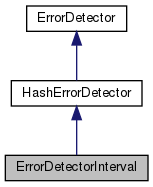
\includegraphics[width=187pt]{class_error_detector_interval__inherit__graph}
\end{center}
\end{figure}


Collaboration diagram for Error\+Detector\+Interval\+:\nopagebreak
\begin{figure}[H]
\begin{center}
\leavevmode
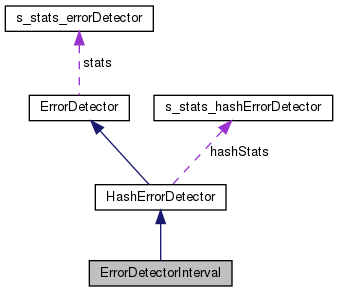
\includegraphics[width=326pt]{class_error_detector_interval__coll__graph}
\end{center}
\end{figure}
\subsection*{Public Member Functions}
\begin{DoxyCompactItemize}
\item 
\hyperlink{class_error_detector_interval_a31b5edf31d0bfa45dfe4d0e4733d59b2}{Error\+Detector\+Interval} ()
\item 
virtual \hyperlink{class_error_detector_interval_a13501d384b2f53dd19dfa1dd9ee0f8fe}{$\sim$\+Error\+Detector\+Interval} ()
\item 
virtual vector$<$ \hyperlink{structures_8h_a83a1d9a070efa5341da84cfd8e28d3e5}{id\+Msg} $>$ \hyperlink{class_error_detector_interval_a6cb5dc28ef7349060d15727e92a6780a}{determine\+And\+Get\+Appended\+Dependencies} (const vector$<$ \hyperlink{structures_8h_a7e7bdc1d2fff8a9436f2f352b2711ed6}{message\+Info} $>$ \&delivered, const \hyperlink{class_probabilistic_clock}{Probabilistic\+Clock} \&clock)
\begin{DoxyCompactList}\small\item\em Determines the causal dependencies to append on the message to broadcast. \end{DoxyCompactList}\item 
bool \hyperlink{class_error_detector_interval_a27cb3ca9d7e5c3ddda9ee5ee66f182ed}{is\+Considered\+As\+Dependency} (const \hyperlink{structures_8h_a7e7bdc1d2fff8a9436f2f352b2711ed6}{message\+Info} \&message, const \hyperlink{structures_8h_a7e7bdc1d2fff8a9436f2f352b2711ed6}{message\+Info} \&possible\+Dep)
\begin{DoxyCompactList}\small\item\em Determines if a message is considered as being a dependency. \end{DoxyCompactList}\item 
bool \hyperlink{class_error_detector_interval_a33bf470042fb65d833fd0f091374a046}{is\+Considered\+As\+Possible\+Dependency} (const \hyperlink{structures_8h_a7e7bdc1d2fff8a9436f2f352b2711ed6}{message\+Info} \&message, const \hyperlink{structures_8h_a7e7bdc1d2fff8a9436f2f352b2711ed6}{message\+Info} \&possible\+Dep)
\begin{DoxyCompactList}\small\item\em Determines if a message is considered as being a possible dependency. \end{DoxyCompactList}\item 
vector$<$ \hyperlink{structures_8h_a83a1d9a070efa5341da84cfd8e28d3e5}{id\+Msg} $>$ \hyperlink{class_error_detector_interval_ae74b39e397894e3485c2f7869fca8fb0}{sort\+Possible\+Dependencies\+Set} (const \hyperlink{structures_8h_a7e7bdc1d2fff8a9436f2f352b2711ed6}{message\+Info} \&message, const vector$<$ \hyperlink{structures_8h_a7e7bdc1d2fff8a9436f2f352b2711ed6}{message\+Info} $>$ \&base\+Combine\+Set)
\begin{DoxyCompactList}\small\item\em Sorts the set of possible dependencies depending on the reception time of messages. \end{DoxyCompactList}\item 
\hyperlink{class_partial_dependencies}{Partial\+Dependencies} \hyperlink{class_error_detector_interval_a9494a918f551eb1efcab39ffd68316d6}{get\+Partial\+Dependencies} (const vector$<$ \hyperlink{structures_8h_a7e7bdc1d2fff8a9436f2f352b2711ed6}{message\+Info} $>$ \&delivered, const \hyperlink{class_probabilistic_clock}{Probabilistic\+Clock} \&clock)
\begin{DoxyCompactList}\small\item\em Get partial dependencies of the message to broadcast. \end{DoxyCompactList}\end{DoxyCompactItemize}
\subsection*{Private Attributes}
\begin{DoxyCompactItemize}
\item 
simtime\+\_\+t \hyperlink{class_error_detector_interval_a24f229a469ae7c4314a948015cddb277}{delta\+TR} = $\ast$(new Sim\+Time(100, S\+I\+M\+T\+I\+M\+E\+\_\+\+MS))
\begin{DoxyCompactList}\small\item\em Assumes that messages received more than 2$\ast$delta\+TR seconds ago are causal dependencies. \end{DoxyCompactList}\item 
simtime\+\_\+t \hyperlink{class_error_detector_interval_adb614477095a1b9753f088f28776c677}{cdelay} = $\ast$(new Sim\+Time(100, S\+I\+M\+T\+I\+M\+E\+\_\+\+MS))
\begin{DoxyCompactList}\small\item\em Communication channel delay. \end{DoxyCompactList}\item 
simtime\+\_\+t \hyperlink{class_error_detector_interval_a2368ba76496cfd25487e150a961bb08b}{delta\+TS} = $\ast$(new Sim\+Time(140, S\+I\+M\+T\+I\+M\+E\+\_\+\+MS))
\begin{DoxyCompactList}\small\item\em Same function as delta\+TR but separates them so that delta\+TR can set to 0 when the message load is low. \end{DoxyCompactList}\end{DoxyCompactItemize}


\subsection{Detailed Description}
Hash-\/based error detector that uses propagation delay hypothesises to determine the causal dependencies of messages. 



\subsection{Constructor \& Destructor Documentation}
\mbox{\Hypertarget{class_error_detector_interval_a31b5edf31d0bfa45dfe4d0e4733d59b2}\label{class_error_detector_interval_a31b5edf31d0bfa45dfe4d0e4733d59b2}} 
\index{Error\+Detector\+Interval@{Error\+Detector\+Interval}!Error\+Detector\+Interval@{Error\+Detector\+Interval}}
\index{Error\+Detector\+Interval@{Error\+Detector\+Interval}!Error\+Detector\+Interval@{Error\+Detector\+Interval}}
\subsubsection{\texorpdfstring{Error\+Detector\+Interval()}{ErrorDetectorInterval()}}
{\footnotesize\ttfamily Error\+Detector\+Interval\+::\+Error\+Detector\+Interval (\begin{DoxyParamCaption}{ }\end{DoxyParamCaption})}

\mbox{\Hypertarget{class_error_detector_interval_a13501d384b2f53dd19dfa1dd9ee0f8fe}\label{class_error_detector_interval_a13501d384b2f53dd19dfa1dd9ee0f8fe}} 
\index{Error\+Detector\+Interval@{Error\+Detector\+Interval}!````~Error\+Detector\+Interval@{$\sim$\+Error\+Detector\+Interval}}
\index{````~Error\+Detector\+Interval@{$\sim$\+Error\+Detector\+Interval}!Error\+Detector\+Interval@{Error\+Detector\+Interval}}
\subsubsection{\texorpdfstring{$\sim$\+Error\+Detector\+Interval()}{~ErrorDetectorInterval()}}
{\footnotesize\ttfamily Error\+Detector\+Interval\+::$\sim$\+Error\+Detector\+Interval (\begin{DoxyParamCaption}{ }\end{DoxyParamCaption})\hspace{0.3cm}{\ttfamily [virtual]}}



\subsection{Member Function Documentation}
\mbox{\Hypertarget{class_error_detector_interval_a6cb5dc28ef7349060d15727e92a6780a}\label{class_error_detector_interval_a6cb5dc28ef7349060d15727e92a6780a}} 
\index{Error\+Detector\+Interval@{Error\+Detector\+Interval}!determine\+And\+Get\+Appended\+Dependencies@{determine\+And\+Get\+Appended\+Dependencies}}
\index{determine\+And\+Get\+Appended\+Dependencies@{determine\+And\+Get\+Appended\+Dependencies}!Error\+Detector\+Interval@{Error\+Detector\+Interval}}
\subsubsection{\texorpdfstring{determine\+And\+Get\+Appended\+Dependencies()}{determineAndGetAppendedDependencies()}}
{\footnotesize\ttfamily vector$<$ \hyperlink{structures_8h_a83a1d9a070efa5341da84cfd8e28d3e5}{id\+Msg} $>$ Error\+Detector\+Interval\+::determine\+And\+Get\+Appended\+Dependencies (\begin{DoxyParamCaption}\item[{const vector$<$ \hyperlink{structures_8h_a7e7bdc1d2fff8a9436f2f352b2711ed6}{message\+Info} $>$ \&}]{delivered,  }\item[{const \hyperlink{class_probabilistic_clock}{Probabilistic\+Clock} \&}]{clock }\end{DoxyParamCaption})\hspace{0.3cm}{\ttfamily [virtual]}}



Determines the causal dependencies to append on the message to broadcast. 


\begin{DoxyParams}{Parameters}
{\em delivered} & Messages the node has delivered, ie the causal dependencies of the message to broadcast. \\
\hline
{\em clock} & The clock appended to the message to broadcast. \\
\hline
\end{DoxyParams}
\begin{DoxyReturn}{Returns}
The set of dependencies that will be appended on the message to broadcast. 
\end{DoxyReturn}


Implements \hyperlink{class_hash_error_detector_ae45353331e29b50a0aa2fc6dd540ed4e}{Hash\+Error\+Detector}.

\mbox{\Hypertarget{class_error_detector_interval_a9494a918f551eb1efcab39ffd68316d6}\label{class_error_detector_interval_a9494a918f551eb1efcab39ffd68316d6}} 
\index{Error\+Detector\+Interval@{Error\+Detector\+Interval}!get\+Partial\+Dependencies@{get\+Partial\+Dependencies}}
\index{get\+Partial\+Dependencies@{get\+Partial\+Dependencies}!Error\+Detector\+Interval@{Error\+Detector\+Interval}}
\subsubsection{\texorpdfstring{get\+Partial\+Dependencies()}{getPartialDependencies()}}
{\footnotesize\ttfamily \hyperlink{class_partial_dependencies}{Partial\+Dependencies} Error\+Detector\+Interval\+::get\+Partial\+Dependencies (\begin{DoxyParamCaption}\item[{const vector$<$ \hyperlink{structures_8h_a7e7bdc1d2fff8a9436f2f352b2711ed6}{message\+Info} $>$ \&}]{delivered,  }\item[{const \hyperlink{class_probabilistic_clock}{Probabilistic\+Clock} \&}]{clock }\end{DoxyParamCaption})\hspace{0.3cm}{\ttfamily [virtual]}}



Get partial dependencies of the message to broadcast. 


\begin{DoxyParams}{Parameters}
{\em delivered} & Messages the node has delivered. \\
\hline
{\em clock} & The clock of the message to broadcast. \\
\hline
\end{DoxyParams}
\begin{DoxyReturn}{Returns}
Partial dependencies of the message to broadcast. 
\end{DoxyReturn}


Implements \hyperlink{class_hash_error_detector_a5b9f7e8a6f63b1582e912102021c2d8d}{Hash\+Error\+Detector}.

\mbox{\Hypertarget{class_error_detector_interval_a27cb3ca9d7e5c3ddda9ee5ee66f182ed}\label{class_error_detector_interval_a27cb3ca9d7e5c3ddda9ee5ee66f182ed}} 
\index{Error\+Detector\+Interval@{Error\+Detector\+Interval}!is\+Considered\+As\+Dependency@{is\+Considered\+As\+Dependency}}
\index{is\+Considered\+As\+Dependency@{is\+Considered\+As\+Dependency}!Error\+Detector\+Interval@{Error\+Detector\+Interval}}
\subsubsection{\texorpdfstring{is\+Considered\+As\+Dependency()}{isConsideredAsDependency()}}
{\footnotesize\ttfamily bool Error\+Detector\+Interval\+::is\+Considered\+As\+Dependency (\begin{DoxyParamCaption}\item[{const \hyperlink{structures_8h_a7e7bdc1d2fff8a9436f2f352b2711ed6}{message\+Info} \&}]{message,  }\item[{const \hyperlink{structures_8h_a7e7bdc1d2fff8a9436f2f352b2711ed6}{message\+Info} \&}]{possible\+Dep }\end{DoxyParamCaption})\hspace{0.3cm}{\ttfamily [virtual]}}



Determines if a message is considered as being a dependency. 


\begin{DoxyParams}{Parameters}
{\em message} & The analyzed message. \\
\hline
{\em possible\+Dep} & The message that is checked to be a dependency. \\
\hline
\end{DoxyParams}
\begin{DoxyReturn}{Returns}
true if possible\+Dep is considered as a dependency of message and false otherwise. 
\end{DoxyReturn}


Implements \hyperlink{class_hash_error_detector_a4693d4d5e327b19f75088cef52bcad7d}{Hash\+Error\+Detector}.

\mbox{\Hypertarget{class_error_detector_interval_a33bf470042fb65d833fd0f091374a046}\label{class_error_detector_interval_a33bf470042fb65d833fd0f091374a046}} 
\index{Error\+Detector\+Interval@{Error\+Detector\+Interval}!is\+Considered\+As\+Possible\+Dependency@{is\+Considered\+As\+Possible\+Dependency}}
\index{is\+Considered\+As\+Possible\+Dependency@{is\+Considered\+As\+Possible\+Dependency}!Error\+Detector\+Interval@{Error\+Detector\+Interval}}
\subsubsection{\texorpdfstring{is\+Considered\+As\+Possible\+Dependency()}{isConsideredAsPossibleDependency()}}
{\footnotesize\ttfamily bool Error\+Detector\+Interval\+::is\+Considered\+As\+Possible\+Dependency (\begin{DoxyParamCaption}\item[{const \hyperlink{structures_8h_a7e7bdc1d2fff8a9436f2f352b2711ed6}{message\+Info} \&}]{message,  }\item[{const \hyperlink{structures_8h_a7e7bdc1d2fff8a9436f2f352b2711ed6}{message\+Info} \&}]{possible\+Dep }\end{DoxyParamCaption})\hspace{0.3cm}{\ttfamily [virtual]}}



Determines if a message is considered as being a possible dependency. 


\begin{DoxyParams}{Parameters}
{\em message} & The analyzed message. \\
\hline
{\em possible\+Dep} & The message that is checked to be a possible dependency. \\
\hline
\end{DoxyParams}
\begin{DoxyReturn}{Returns}
true if possible\+Dep is considered as a possible dependency of message and false otherwise. 
\end{DoxyReturn}


Implements \hyperlink{class_hash_error_detector_ac0a25b9c1e27f98223869d11ca46d18f}{Hash\+Error\+Detector}.

\mbox{\Hypertarget{class_error_detector_interval_ae74b39e397894e3485c2f7869fca8fb0}\label{class_error_detector_interval_ae74b39e397894e3485c2f7869fca8fb0}} 
\index{Error\+Detector\+Interval@{Error\+Detector\+Interval}!sort\+Possible\+Dependencies\+Set@{sort\+Possible\+Dependencies\+Set}}
\index{sort\+Possible\+Dependencies\+Set@{sort\+Possible\+Dependencies\+Set}!Error\+Detector\+Interval@{Error\+Detector\+Interval}}
\subsubsection{\texorpdfstring{sort\+Possible\+Dependencies\+Set()}{sortPossibleDependenciesSet()}}
{\footnotesize\ttfamily vector$<$ \hyperlink{structures_8h_a83a1d9a070efa5341da84cfd8e28d3e5}{id\+Msg} $>$ Error\+Detector\+Interval\+::sort\+Possible\+Dependencies\+Set (\begin{DoxyParamCaption}\item[{const \hyperlink{structures_8h_a7e7bdc1d2fff8a9436f2f352b2711ed6}{message\+Info} \&}]{message,  }\item[{const vector$<$ \hyperlink{structures_8h_a7e7bdc1d2fff8a9436f2f352b2711ed6}{message\+Info} $>$ \&}]{base\+Combine\+Set }\end{DoxyParamCaption})\hspace{0.3cm}{\ttfamily [virtual]}}



Sorts the set of possible dependencies depending on the reception time of messages. 


\begin{DoxyParams}{Parameters}
{\em message} & Message to deliver. \\
\hline
{\em base\+Combine\+Set} & Set of possible dependencies to order. \\
\hline
\end{DoxyParams}
\begin{DoxyReturn}{Returns}
Sorted set of possible dependencies in increasing order of probability of being a dependency of message. 
\end{DoxyReturn}


Implements \hyperlink{class_hash_error_detector_aa7952b99e47ca7cef6dae2a271885599}{Hash\+Error\+Detector}.



\subsection{Member Data Documentation}
\mbox{\Hypertarget{class_error_detector_interval_adb614477095a1b9753f088f28776c677}\label{class_error_detector_interval_adb614477095a1b9753f088f28776c677}} 
\index{Error\+Detector\+Interval@{Error\+Detector\+Interval}!cdelay@{cdelay}}
\index{cdelay@{cdelay}!Error\+Detector\+Interval@{Error\+Detector\+Interval}}
\subsubsection{\texorpdfstring{cdelay}{cdelay}}
{\footnotesize\ttfamily simtime\+\_\+t Error\+Detector\+Interval\+::cdelay = $\ast$(new Sim\+Time(100, S\+I\+M\+T\+I\+M\+E\+\_\+\+MS))\hspace{0.3cm}{\ttfamily [private]}}



Communication channel delay. 

\mbox{\Hypertarget{class_error_detector_interval_a24f229a469ae7c4314a948015cddb277}\label{class_error_detector_interval_a24f229a469ae7c4314a948015cddb277}} 
\index{Error\+Detector\+Interval@{Error\+Detector\+Interval}!delta\+TR@{delta\+TR}}
\index{delta\+TR@{delta\+TR}!Error\+Detector\+Interval@{Error\+Detector\+Interval}}
\subsubsection{\texorpdfstring{delta\+TR}{deltaTR}}
{\footnotesize\ttfamily simtime\+\_\+t Error\+Detector\+Interval\+::delta\+TR = $\ast$(new Sim\+Time(100, S\+I\+M\+T\+I\+M\+E\+\_\+\+MS))\hspace{0.3cm}{\ttfamily [private]}}



Assumes that messages received more than 2$\ast$delta\+TR seconds ago are causal dependencies. 

Do not take a value that is too high. \mbox{\Hypertarget{class_error_detector_interval_a2368ba76496cfd25487e150a961bb08b}\label{class_error_detector_interval_a2368ba76496cfd25487e150a961bb08b}} 
\index{Error\+Detector\+Interval@{Error\+Detector\+Interval}!delta\+TS@{delta\+TS}}
\index{delta\+TS@{delta\+TS}!Error\+Detector\+Interval@{Error\+Detector\+Interval}}
\subsubsection{\texorpdfstring{delta\+TS}{deltaTS}}
{\footnotesize\ttfamily simtime\+\_\+t Error\+Detector\+Interval\+::delta\+TS = $\ast$(new Sim\+Time(140, S\+I\+M\+T\+I\+M\+E\+\_\+\+MS))\hspace{0.3cm}{\ttfamily [private]}}



Same function as delta\+TR but separates them so that delta\+TR can set to 0 when the message load is low. 



The documentation for this class was generated from the following files\+:\begin{DoxyCompactItemize}
\item 
src/\+Detectors/\hyperlink{_hash_error_detector_interval_8h}{Hash\+Error\+Detector\+Interval.\+h}\item 
src/\+Detectors/\hyperlink{_hash_error_detector_interval_8cc}{Hash\+Error\+Detector\+Interval.\+cc}\end{DoxyCompactItemize}

\hypertarget{class_hash_error_detector}{}\section{Hash\+Error\+Detector Class Reference}
\label{class_hash_error_detector}\index{Hash\+Error\+Detector@{Hash\+Error\+Detector}}


Base class of Hash-\/based error detectors.  




{\ttfamily \#include $<$Hash\+Error\+Detector.\+h$>$}



Inheritance diagram for Hash\+Error\+Detector\+:
\nopagebreak
\begin{figure}[H]
\begin{center}
\leavevmode
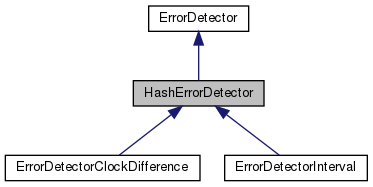
\includegraphics[width=350pt]{class_hash_error_detector__inherit__graph}
\end{center}
\end{figure}


Collaboration diagram for Hash\+Error\+Detector\+:
\nopagebreak
\begin{figure}[H]
\begin{center}
\leavevmode
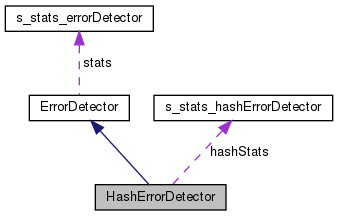
\includegraphics[width=326pt]{class_hash_error_detector__coll__graph}
\end{center}
\end{figure}
\subsection*{Public Member Functions}
\begin{DoxyCompactItemize}
\item 
\hyperlink{class_hash_error_detector_a008bd7bd3f8d202334afd51a71cbbdae}{Hash\+Error\+Detector} ()
\item 
virtual \hyperlink{class_hash_error_detector_a187ba4d9f902ecaa0ff8b92ec531d3f4}{$\sim$\+Hash\+Error\+Detector} ()
\item 
virtual bool \hyperlink{class_hash_error_detector_a1c7fe649a34cf7e139ce53a248dce748}{test} (\hyperlink{structures_8h_a7e7bdc1d2fff8a9436f2f352b2711ed6}{message\+Info} message, const vector$<$ unsigned int $>$ \&incremented\+Clock\+Entries, const \hyperlink{class_probabilistic_clock}{Probabilistic\+Clock} \&process\+Clock, const \hyperlink{class_total_dependencies}{Total\+Dependencies} \&process\+Dependencies, \hyperlink{class_controller}{Controller} $\ast$control, \hyperlink{class_simulation_parameters}{Simulation\+Parameters} $\ast$params, const vector$<$ \hyperlink{structures_8h_a7e7bdc1d2fff8a9436f2f352b2711ed6}{message\+Info} $>$ \&delivered)
\begin{DoxyCompactList}\small\item\em Test executed on a message to determine if it can be causally delivered. \end{DoxyCompactList}\item 
bool \hyperlink{class_hash_error_detector_a851c562e49f608ec3fe3e984db27bfca}{hash\+Partial\+Dependencies} (const \hyperlink{structures_8h_a7e7bdc1d2fff8a9436f2f352b2711ed6}{message\+Info} \&message, const vector$<$ \hyperlink{structures_8h_a7e7bdc1d2fff8a9436f2f352b2711ed6}{message\+Info} $>$ \&delivered, const vector$<$ unsigned int $>$ \&incremented\+Clock\+Entries, \hyperlink{class_controller}{Controller} $\ast$controller, \hyperlink{class_simulation_parameters}{Simulation\+Parameters} $\ast$params)
\begin{DoxyCompactList}\small\item\em Test executed on a message when using partial dependencies to determine if it can be causally delivered. \end{DoxyCompactList}\item 
bool \hyperlink{class_hash_error_detector_a13dd5fae3ca4898bd91d1801beed24a4}{hash\+Total\+Dependencies} (const \hyperlink{structures_8h_a7e7bdc1d2fff8a9436f2f352b2711ed6}{message\+Info} \&message, const vector$<$ \hyperlink{structures_8h_a7e7bdc1d2fff8a9436f2f352b2711ed6}{message\+Info} $>$ \&delivered, const vector$<$ unsigned int $>$ \&incremented\+Clock\+Entries, const \hyperlink{class_total_dependencies}{Total\+Dependencies} \&process\+Dependencies, \hyperlink{class_controller}{Controller} $\ast$controller, \hyperlink{class_simulation_parameters}{Simulation\+Parameters} $\ast$params)
\begin{DoxyCompactList}\small\item\em Test executed on a message when using total dependencies to determine if it can be causally delivered. \end{DoxyCompactList}\item 
bool \hyperlink{class_hash_error_detector_a93b22ebde71c18f801319b33ce30899c}{hash\+Is\+Equal} (size\+\_\+t message\+Hash, size\+\_\+t dependencies\+Hash, unsigned int nb\+Computed\+Hashes)
\begin{DoxyCompactList}\small\item\em Verifies if the hash of the message and dependencies set are equal. \end{DoxyCompactList}\item 
\hyperlink{class_total_dependencies}{Total\+Dependencies} \hyperlink{class_hash_error_detector_a09b0d73b3a717ddf850fe644848c15c6}{create\+Base\+Dependencies} (const \hyperlink{structures_8h_a7e7bdc1d2fff8a9436f2f352b2711ed6}{message\+Info} \&message, const vector$<$ \hyperlink{structures_8h_a7e7bdc1d2fff8a9436f2f352b2711ed6}{message\+Info} $>$ \&delivered, const vector$<$ unsigned int $>$ \&incremented\+Clock\+Entries, const \hyperlink{class_total_dependencies}{Total\+Dependencies} \&process\+Dependencies)
\begin{DoxyCompactList}\small\item\em Creates the set of messages that are considered as dependencies of the message to deliver. \end{DoxyCompactList}\item 
bool \hyperlink{class_hash_error_detector_aaaceeb3d2d27d5f3c85a9b80f959e0fe}{is\+Possible\+Dependency} (const \hyperlink{structures_8h_a7e7bdc1d2fff8a9436f2f352b2711ed6}{message\+Info} \&message, const \hyperlink{structures_8h_a7e7bdc1d2fff8a9436f2f352b2711ed6}{message\+Info} \&possible\+Dep)
\begin{DoxyCompactList}\small\item\em Determines if a message is a possible dependency of another message. \end{DoxyCompactList}\item 
vector$<$ \hyperlink{structures_8h_a7e7bdc1d2fff8a9436f2f352b2711ed6}{message\+Info} $>$ \hyperlink{class_hash_error_detector_ae8605d778886baa20648a9f5955c5943}{create\+Possible\+Dependencies\+Set} (const \hyperlink{structures_8h_a7e7bdc1d2fff8a9436f2f352b2711ed6}{message\+Info} \&message, const vector$<$ \hyperlink{structures_8h_a7e7bdc1d2fff8a9436f2f352b2711ed6}{message\+Info} $>$ \&message\+To\+Choose\+From, const vector$<$ unsigned int $>$ \&incremented\+Clock\+Entries, \hyperlink{class_controller}{Controller} $\ast$controller)
\begin{DoxyCompactList}\small\item\em Creates the set of messages that are considered as possible dependencies of the message to deliver. \end{DoxyCompactList}\item 
void \hyperlink{class_hash_error_detector_a007d537bdfd329c6b23b432b58d4cf4c}{incrementnb\+Msg\+Wrongly\+Considered\+Causal\+Dep} (unsigned int entry)
\begin{DoxyCompactList}\small\item\em Increments the vector nb\+Msg\+Wrongly\+Considered\+Causal\+Dep while avoiding out of array bounds increments. \end{DoxyCompactList}\item 
void \hyperlink{class_hash_error_detector_a08b4518822a6beff6845da4dd36bfba1}{incrementnb\+Msg\+To\+Combine} (unsigned int entry)
\begin{DoxyCompactList}\small\item\em Increments the vector nb\+Msg\+To\+Combine while avoiding out of array bounds increments. \end{DoxyCompactList}\item 
void \hyperlink{class_hash_error_detector_a6aa56dfbb555e15093bd5d93a683fa42}{incrementnb\+Operations\+For\+Hash} (unsigned int entry)
\begin{DoxyCompactList}\small\item\em Increments the vector nb\+Operations\+For\+Hash while avoiding out of array bounds increments. \end{DoxyCompactList}\item 
size\+\_\+t \hyperlink{class_hash_error_detector_afcad668b4f0ca1c838b40a3c0584c1ee}{hash\+Total\+Dependencies} (const \hyperlink{class_total_dependencies}{Total\+Dependencies} \&dependencies)
\begin{DoxyCompactList}\small\item\em Hashes total dependencies. \end{DoxyCompactList}\item 
size\+\_\+t \hyperlink{class_hash_error_detector_aed8b0c6d17198a493e5b89f69c2e8713}{hash\+Partial\+Dependencies} (const \hyperlink{class_partial_dependencies}{Partial\+Dependencies} \&dependencies)
\begin{DoxyCompactList}\small\item\em Hashes partial dependencies. \end{DoxyCompactList}\item 
size\+\_\+t \hyperlink{class_hash_error_detector_a37d0ee7d8a01b530a03262e4483c53d9}{hash\+Dependencies} (const vector$<$ unsigned int $>$ \&dependencies)
\begin{DoxyCompactList}\small\item\em Hashes the set of dependencies. \end{DoxyCompactList}\item 
size\+\_\+t \hyperlink{class_hash_error_detector_aa0b6a85ef4078e4851cd56b612a539c5}{hashingF} (const vector$<$ uint32\+\_\+t $>$ \&vec)
\begin{DoxyCompactList}\small\item\em Hashes a vector. \end{DoxyCompactList}\item 
\hyperlink{class_app_msg}{App\+Msg} $\ast$ \hyperlink{class_hash_error_detector_a2b1dad6a83a08fd7ce88e32f84638459}{prepare\+Message} (\hyperlink{class_app_msg}{App\+Msg} $\ast$m, const vector$<$ \hyperlink{structures_8h_a7e7bdc1d2fff8a9436f2f352b2711ed6}{message\+Info} $>$ \&delivered, const \hyperlink{class_probabilistic_clock}{Probabilistic\+Clock} \&clock, const \hyperlink{class_total_dependencies}{Total\+Dependencies} \&process\+Dependencies)
\begin{DoxyCompactList}\small\item\em Prepares the message to broadcast when using hash-\/based error detectors. \end{DoxyCompactList}\item 
virtual bool \hyperlink{class_hash_error_detector_a4693d4d5e327b19f75088cef52bcad7d}{is\+Considered\+As\+Dependency} (const \hyperlink{structures_8h_a7e7bdc1d2fff8a9436f2f352b2711ed6}{message\+Info} \&message, const \hyperlink{structures_8h_a7e7bdc1d2fff8a9436f2f352b2711ed6}{message\+Info} \&possible\+Dep)=0
\item 
virtual bool \hyperlink{class_hash_error_detector_ac0a25b9c1e27f98223869d11ca46d18f}{is\+Considered\+As\+Possible\+Dependency} (const \hyperlink{structures_8h_a7e7bdc1d2fff8a9436f2f352b2711ed6}{message\+Info} \&message, const \hyperlink{structures_8h_a7e7bdc1d2fff8a9436f2f352b2711ed6}{message\+Info} \&possible\+Dep)=0
\item 
virtual vector$<$ \hyperlink{structures_8h_a83a1d9a070efa5341da84cfd8e28d3e5}{id\+Msg} $>$ \hyperlink{class_hash_error_detector_aa7952b99e47ca7cef6dae2a271885599}{sort\+Possible\+Dependencies\+Set} (const \hyperlink{structures_8h_a7e7bdc1d2fff8a9436f2f352b2711ed6}{message\+Info} \&message, const vector$<$ \hyperlink{structures_8h_a7e7bdc1d2fff8a9436f2f352b2711ed6}{message\+Info} $>$ \&base\+Combine\+Set)=0
\item 
virtual \hyperlink{class_partial_dependencies}{Partial\+Dependencies} \hyperlink{class_hash_error_detector_a5b9f7e8a6f63b1582e912102021c2d8d}{get\+Partial\+Dependencies} (const vector$<$ \hyperlink{structures_8h_a7e7bdc1d2fff8a9436f2f352b2711ed6}{message\+Info} $>$ \&delivered, const \hyperlink{class_probabilistic_clock}{Probabilistic\+Clock} \&clock)=0
\item 
virtual vector$<$ \hyperlink{structures_8h_a83a1d9a070efa5341da84cfd8e28d3e5}{id\+Msg} $>$ \hyperlink{class_hash_error_detector_ae45353331e29b50a0aa2fc6dd540ed4e}{determine\+And\+Get\+Appended\+Dependencies} (const vector$<$ \hyperlink{structures_8h_a7e7bdc1d2fff8a9436f2f352b2711ed6}{message\+Info} $>$ \&delivered, const \hyperlink{class_probabilistic_clock}{Probabilistic\+Clock} \&clock)=0
\end{DoxyCompactItemize}
\subsection*{Private Attributes}
\begin{DoxyCompactItemize}
\item 
hash$<$ string $>$ \hyperlink{class_hash_error_detector_a5193286d834f087e03b7299e81b60509}{hasher}
\begin{DoxyCompactList}\small\item\em Used to compute hashes. \end{DoxyCompactList}\item 
\hyperlink{_hash_error_detector_8h_afcf148bcfe372c25deda29220815b9e0}{stats\+\_\+hash\+Error\+Detector} \hyperlink{class_hash_error_detector_aec82c653679515b306b34eb075cf37fd}{hash\+Stats}
\begin{DoxyCompactList}\small\item\em Statistics about hash-\/based error detectors. \end{DoxyCompactList}\end{DoxyCompactItemize}
\subsection*{Static Private Attributes}
\begin{DoxyCompactItemize}
\item 
static map$<$ int, vector$<$ unsigned int $>$ $>$ \hyperlink{class_hash_error_detector_a662a2baf62e11d8e2468aee44b9b168e}{collision\+Controller}
\begin{DoxyCompactList}\small\item\em Used to detect collisions when hashing dependencies sets, ie detect when different dependencies sets have the same hash. \end{DoxyCompactList}\end{DoxyCompactItemize}
\subsection*{Friends}
\begin{DoxyCompactItemize}
\item 
class \hyperlink{class_hash_error_detector_a129f65b6976377739eb6231b6962985e}{Stats}
\item 
class \hyperlink{class_hash_error_detector_a4a759c82473f06c7e89c3d75a509a390}{Node\+With\+Recovery\+Test}
\end{DoxyCompactItemize}


\subsection{Detailed Description}
Base class of Hash-\/based error detectors. 



\subsection{Constructor \& Destructor Documentation}
\mbox{\Hypertarget{class_hash_error_detector_a008bd7bd3f8d202334afd51a71cbbdae}\label{class_hash_error_detector_a008bd7bd3f8d202334afd51a71cbbdae}} 
\index{Hash\+Error\+Detector@{Hash\+Error\+Detector}!Hash\+Error\+Detector@{Hash\+Error\+Detector}}
\index{Hash\+Error\+Detector@{Hash\+Error\+Detector}!Hash\+Error\+Detector@{Hash\+Error\+Detector}}
\subsubsection{\texorpdfstring{Hash\+Error\+Detector()}{HashErrorDetector()}}
{\footnotesize\ttfamily Hash\+Error\+Detector\+::\+Hash\+Error\+Detector (\begin{DoxyParamCaption}{ }\end{DoxyParamCaption})}

\mbox{\Hypertarget{class_hash_error_detector_a187ba4d9f902ecaa0ff8b92ec531d3f4}\label{class_hash_error_detector_a187ba4d9f902ecaa0ff8b92ec531d3f4}} 
\index{Hash\+Error\+Detector@{Hash\+Error\+Detector}!````~Hash\+Error\+Detector@{$\sim$\+Hash\+Error\+Detector}}
\index{````~Hash\+Error\+Detector@{$\sim$\+Hash\+Error\+Detector}!Hash\+Error\+Detector@{Hash\+Error\+Detector}}
\subsubsection{\texorpdfstring{$\sim$\+Hash\+Error\+Detector()}{~HashErrorDetector()}}
{\footnotesize\ttfamily Hash\+Error\+Detector\+::$\sim$\+Hash\+Error\+Detector (\begin{DoxyParamCaption}{ }\end{DoxyParamCaption})\hspace{0.3cm}{\ttfamily [virtual]}}



\subsection{Member Function Documentation}
\mbox{\Hypertarget{class_hash_error_detector_a09b0d73b3a717ddf850fe644848c15c6}\label{class_hash_error_detector_a09b0d73b3a717ddf850fe644848c15c6}} 
\index{Hash\+Error\+Detector@{Hash\+Error\+Detector}!create\+Base\+Dependencies@{create\+Base\+Dependencies}}
\index{create\+Base\+Dependencies@{create\+Base\+Dependencies}!Hash\+Error\+Detector@{Hash\+Error\+Detector}}
\subsubsection{\texorpdfstring{create\+Base\+Dependencies()}{createBaseDependencies()}}
{\footnotesize\ttfamily \hyperlink{class_total_dependencies}{Total\+Dependencies} Hash\+Error\+Detector\+::create\+Base\+Dependencies (\begin{DoxyParamCaption}\item[{const \hyperlink{structures_8h_a7e7bdc1d2fff8a9436f2f352b2711ed6}{message\+Info} \&}]{message,  }\item[{const vector$<$ \hyperlink{structures_8h_a7e7bdc1d2fff8a9436f2f352b2711ed6}{message\+Info} $>$ \&}]{delivered,  }\item[{const vector$<$ unsigned int $>$ \&}]{incremented\+Clock\+Entries,  }\item[{const \hyperlink{class_total_dependencies}{Total\+Dependencies} \&}]{process\+Dependencies }\end{DoxyParamCaption})}



Creates the set of messages that are considered as dependencies of the message to deliver. 


\begin{DoxyParams}{Parameters}
{\em message} & Message to deliver. \\
\hline
{\em delivered} & Messages delivered by the current node. \\
\hline
{\em incremented\+Clock\+Entries} & Entries the sender node of message incremented when broadcasting message. \\
\hline
{\em process\+Dependencies} & Tracker of the delivered messages of the current node. \\
\hline
\end{DoxyParams}
\begin{DoxyReturn}{Returns}
The set of messages that are considered as being dependencies of message. 
\end{DoxyReturn}
\mbox{\Hypertarget{class_hash_error_detector_ae8605d778886baa20648a9f5955c5943}\label{class_hash_error_detector_ae8605d778886baa20648a9f5955c5943}} 
\index{Hash\+Error\+Detector@{Hash\+Error\+Detector}!create\+Possible\+Dependencies\+Set@{create\+Possible\+Dependencies\+Set}}
\index{create\+Possible\+Dependencies\+Set@{create\+Possible\+Dependencies\+Set}!Hash\+Error\+Detector@{Hash\+Error\+Detector}}
\subsubsection{\texorpdfstring{create\+Possible\+Dependencies\+Set()}{createPossibleDependenciesSet()}}
{\footnotesize\ttfamily vector$<$ \hyperlink{structures_8h_a7e7bdc1d2fff8a9436f2f352b2711ed6}{message\+Info} $>$ Hash\+Error\+Detector\+::create\+Possible\+Dependencies\+Set (\begin{DoxyParamCaption}\item[{const \hyperlink{structures_8h_a7e7bdc1d2fff8a9436f2f352b2711ed6}{message\+Info} \&}]{message,  }\item[{const vector$<$ \hyperlink{structures_8h_a7e7bdc1d2fff8a9436f2f352b2711ed6}{message\+Info} $>$ \&}]{message\+To\+Choose\+From,  }\item[{const vector$<$ unsigned int $>$ \&}]{incremented\+Clock\+Entries,  }\item[{\hyperlink{class_controller}{Controller} $\ast$}]{controller }\end{DoxyParamCaption})}



Creates the set of messages that are considered as possible dependencies of the message to deliver. 


\begin{DoxyParams}{Parameters}
{\em message} & Message to deliver. \\
\hline
{\em message\+To\+Choose\+From} & Set containing the messages that might be possible dependencies of message. \\
\hline
{\em incremented\+Clock\+Entries} & Entries the sender node of message incremented when broadcasting message. \\
\hline
{\em controller} & \hyperlink{class_controller}{Controller} module. \\
\hline
\end{DoxyParams}
\begin{DoxyReturn}{Returns}
The set of messages that are considered as possible dependencies of message. 
\end{DoxyReturn}
\mbox{\Hypertarget{class_hash_error_detector_ae45353331e29b50a0aa2fc6dd540ed4e}\label{class_hash_error_detector_ae45353331e29b50a0aa2fc6dd540ed4e}} 
\index{Hash\+Error\+Detector@{Hash\+Error\+Detector}!determine\+And\+Get\+Appended\+Dependencies@{determine\+And\+Get\+Appended\+Dependencies}}
\index{determine\+And\+Get\+Appended\+Dependencies@{determine\+And\+Get\+Appended\+Dependencies}!Hash\+Error\+Detector@{Hash\+Error\+Detector}}
\subsubsection{\texorpdfstring{determine\+And\+Get\+Appended\+Dependencies()}{determineAndGetAppendedDependencies()}}
{\footnotesize\ttfamily virtual vector$<$\hyperlink{structures_8h_a83a1d9a070efa5341da84cfd8e28d3e5}{id\+Msg}$>$ Hash\+Error\+Detector\+::determine\+And\+Get\+Appended\+Dependencies (\begin{DoxyParamCaption}\item[{const vector$<$ \hyperlink{structures_8h_a7e7bdc1d2fff8a9436f2f352b2711ed6}{message\+Info} $>$ \&}]{delivered,  }\item[{const \hyperlink{class_probabilistic_clock}{Probabilistic\+Clock} \&}]{clock }\end{DoxyParamCaption})\hspace{0.3cm}{\ttfamily [pure virtual]}}



Implemented in \hyperlink{class_error_detector_clock_difference_a15406c8d7652f3b9358b1958d3723933}{Error\+Detector\+Clock\+Difference}, and \hyperlink{class_error_detector_interval_a6cb5dc28ef7349060d15727e92a6780a}{Error\+Detector\+Interval}.

\mbox{\Hypertarget{class_hash_error_detector_a5b9f7e8a6f63b1582e912102021c2d8d}\label{class_hash_error_detector_a5b9f7e8a6f63b1582e912102021c2d8d}} 
\index{Hash\+Error\+Detector@{Hash\+Error\+Detector}!get\+Partial\+Dependencies@{get\+Partial\+Dependencies}}
\index{get\+Partial\+Dependencies@{get\+Partial\+Dependencies}!Hash\+Error\+Detector@{Hash\+Error\+Detector}}
\subsubsection{\texorpdfstring{get\+Partial\+Dependencies()}{getPartialDependencies()}}
{\footnotesize\ttfamily virtual \hyperlink{class_partial_dependencies}{Partial\+Dependencies} Hash\+Error\+Detector\+::get\+Partial\+Dependencies (\begin{DoxyParamCaption}\item[{const vector$<$ \hyperlink{structures_8h_a7e7bdc1d2fff8a9436f2f352b2711ed6}{message\+Info} $>$ \&}]{delivered,  }\item[{const \hyperlink{class_probabilistic_clock}{Probabilistic\+Clock} \&}]{clock }\end{DoxyParamCaption})\hspace{0.3cm}{\ttfamily [pure virtual]}}



Implemented in \hyperlink{class_error_detector_clock_difference_a26f4c2905859947201d0a18146f2e961}{Error\+Detector\+Clock\+Difference}, and \hyperlink{class_error_detector_interval_a9494a918f551eb1efcab39ffd68316d6}{Error\+Detector\+Interval}.

\mbox{\Hypertarget{class_hash_error_detector_a37d0ee7d8a01b530a03262e4483c53d9}\label{class_hash_error_detector_a37d0ee7d8a01b530a03262e4483c53d9}} 
\index{Hash\+Error\+Detector@{Hash\+Error\+Detector}!hash\+Dependencies@{hash\+Dependencies}}
\index{hash\+Dependencies@{hash\+Dependencies}!Hash\+Error\+Detector@{Hash\+Error\+Detector}}
\subsubsection{\texorpdfstring{hash\+Dependencies()}{hashDependencies()}}
{\footnotesize\ttfamily size\+\_\+t Hash\+Error\+Detector\+::hash\+Dependencies (\begin{DoxyParamCaption}\item[{const vector$<$ unsigned int $>$ \&}]{dependencies }\end{DoxyParamCaption})}



Hashes the set of dependencies. 


\begin{DoxyParams}{Parameters}
{\em dependencies} & The dependencies to hash. \\
\hline
\end{DoxyParams}
\begin{DoxyReturn}{Returns}
The hash. 
\end{DoxyReturn}
\mbox{\Hypertarget{class_hash_error_detector_aa0b6a85ef4078e4851cd56b612a539c5}\label{class_hash_error_detector_aa0b6a85ef4078e4851cd56b612a539c5}} 
\index{Hash\+Error\+Detector@{Hash\+Error\+Detector}!hashingF@{hashingF}}
\index{hashingF@{hashingF}!Hash\+Error\+Detector@{Hash\+Error\+Detector}}
\subsubsection{\texorpdfstring{hashing\+F()}{hashingF()}}
{\footnotesize\ttfamily size\+\_\+t Hash\+Error\+Detector\+::hashingF (\begin{DoxyParamCaption}\item[{const vector$<$ uint32\+\_\+t $>$ \&}]{vec }\end{DoxyParamCaption})}



Hashes a vector. 


\begin{DoxyParams}{Parameters}
{\em vec} & The vector to hash. \\
\hline
\end{DoxyParams}
\begin{DoxyReturn}{Returns}
The hash. 
\end{DoxyReturn}
\mbox{\Hypertarget{class_hash_error_detector_a93b22ebde71c18f801319b33ce30899c}\label{class_hash_error_detector_a93b22ebde71c18f801319b33ce30899c}} 
\index{Hash\+Error\+Detector@{Hash\+Error\+Detector}!hash\+Is\+Equal@{hash\+Is\+Equal}}
\index{hash\+Is\+Equal@{hash\+Is\+Equal}!Hash\+Error\+Detector@{Hash\+Error\+Detector}}
\subsubsection{\texorpdfstring{hash\+Is\+Equal()}{hashIsEqual()}}
{\footnotesize\ttfamily bool Hash\+Error\+Detector\+::hash\+Is\+Equal (\begin{DoxyParamCaption}\item[{size\+\_\+t}]{message\+Hash,  }\item[{size\+\_\+t}]{dependencies\+Hash,  }\item[{unsigned int}]{nb\+Computed\+Hashes }\end{DoxyParamCaption})}



Verifies if the hash of the message and dependencies set are equal. 


\begin{DoxyParams}{Parameters}
{\em message\+Hash} & Hash of the message to deliver. \\
\hline
{\em dependencies\+Hash} & Hash of the dependencies set. \\
\hline
{\em nb\+Computed\+Hashes} & Number of computed hashes in the current hash computation. \\
\hline
\end{DoxyParams}
\begin{DoxyReturn}{Returns}
true if the hash is equal, false otherwise. 
\end{DoxyReturn}
\mbox{\Hypertarget{class_hash_error_detector_a851c562e49f608ec3fe3e984db27bfca}\label{class_hash_error_detector_a851c562e49f608ec3fe3e984db27bfca}} 
\index{Hash\+Error\+Detector@{Hash\+Error\+Detector}!hash\+Partial\+Dependencies@{hash\+Partial\+Dependencies}}
\index{hash\+Partial\+Dependencies@{hash\+Partial\+Dependencies}!Hash\+Error\+Detector@{Hash\+Error\+Detector}}
\subsubsection{\texorpdfstring{hash\+Partial\+Dependencies()}{hashPartialDependencies()}\hspace{0.1cm}{\footnotesize\ttfamily [1/2]}}
{\footnotesize\ttfamily bool Hash\+Error\+Detector\+::hash\+Partial\+Dependencies (\begin{DoxyParamCaption}\item[{const \hyperlink{structures_8h_a7e7bdc1d2fff8a9436f2f352b2711ed6}{message\+Info} \&}]{message,  }\item[{const vector$<$ \hyperlink{structures_8h_a7e7bdc1d2fff8a9436f2f352b2711ed6}{message\+Info} $>$ \&}]{delivered,  }\item[{const vector$<$ unsigned int $>$ \&}]{incremented\+Clock\+Entries,  }\item[{\hyperlink{class_controller}{Controller} $\ast$}]{controller,  }\item[{\hyperlink{class_simulation_parameters}{Simulation\+Parameters} $\ast$}]{params }\end{DoxyParamCaption})}



Test executed on a message when using partial dependencies to determine if it can be causally delivered. 


\begin{DoxyParams}{Parameters}
{\em message} & Message to deliver. \\
\hline
{\em delivered} & Messages delivered by the current node. \\
\hline
{\em incremented\+Clock\+Entries} & Entries the sender node of message incremented when broadcasting message. \\
\hline
{\em controller} & \hyperlink{class_controller}{Controller} module. \\
\hline
{\em params} & Simulation parameters. \\
\hline
\end{DoxyParams}
\begin{DoxyReturn}{Returns}
true if the error detector concludes that the message can be causally delivered and false otherwise. 
\end{DoxyReturn}
\mbox{\Hypertarget{class_hash_error_detector_aed8b0c6d17198a493e5b89f69c2e8713}\label{class_hash_error_detector_aed8b0c6d17198a493e5b89f69c2e8713}} 
\index{Hash\+Error\+Detector@{Hash\+Error\+Detector}!hash\+Partial\+Dependencies@{hash\+Partial\+Dependencies}}
\index{hash\+Partial\+Dependencies@{hash\+Partial\+Dependencies}!Hash\+Error\+Detector@{Hash\+Error\+Detector}}
\subsubsection{\texorpdfstring{hash\+Partial\+Dependencies()}{hashPartialDependencies()}\hspace{0.1cm}{\footnotesize\ttfamily [2/2]}}
{\footnotesize\ttfamily size\+\_\+t Hash\+Error\+Detector\+::hash\+Partial\+Dependencies (\begin{DoxyParamCaption}\item[{const \hyperlink{class_partial_dependencies}{Partial\+Dependencies} \&}]{dependencies }\end{DoxyParamCaption})}



Hashes partial dependencies. 


\begin{DoxyParams}{Parameters}
{\em dependencies} & The partial dependencies to hash. \\
\hline
\end{DoxyParams}
\begin{DoxyReturn}{Returns}
The hash. 
\end{DoxyReturn}
\mbox{\Hypertarget{class_hash_error_detector_a13dd5fae3ca4898bd91d1801beed24a4}\label{class_hash_error_detector_a13dd5fae3ca4898bd91d1801beed24a4}} 
\index{Hash\+Error\+Detector@{Hash\+Error\+Detector}!hash\+Total\+Dependencies@{hash\+Total\+Dependencies}}
\index{hash\+Total\+Dependencies@{hash\+Total\+Dependencies}!Hash\+Error\+Detector@{Hash\+Error\+Detector}}
\subsubsection{\texorpdfstring{hash\+Total\+Dependencies()}{hashTotalDependencies()}\hspace{0.1cm}{\footnotesize\ttfamily [1/2]}}
{\footnotesize\ttfamily bool Hash\+Error\+Detector\+::hash\+Total\+Dependencies (\begin{DoxyParamCaption}\item[{const \hyperlink{structures_8h_a7e7bdc1d2fff8a9436f2f352b2711ed6}{message\+Info} \&}]{message,  }\item[{const vector$<$ \hyperlink{structures_8h_a7e7bdc1d2fff8a9436f2f352b2711ed6}{message\+Info} $>$ \&}]{delivered,  }\item[{const vector$<$ unsigned int $>$ \&}]{incremented\+Clock\+Entries,  }\item[{const \hyperlink{class_total_dependencies}{Total\+Dependencies} \&}]{process\+Dependencies,  }\item[{\hyperlink{class_controller}{Controller} $\ast$}]{controller,  }\item[{\hyperlink{class_simulation_parameters}{Simulation\+Parameters} $\ast$}]{params }\end{DoxyParamCaption})}



Test executed on a message when using total dependencies to determine if it can be causally delivered. 


\begin{DoxyParams}{Parameters}
{\em message} & Message to deliver. \\
\hline
{\em delivered} & Messages delivered by the current node. \\
\hline
{\em incremented\+Clock\+Entries} & Entries the sender node of message incremented when broadcasting message. \\
\hline
{\em process\+Dependencies} & Tracker of the delivered messages of the current node. \\
\hline
{\em controller} & \hyperlink{class_controller}{Controller} module. \\
\hline
{\em params} & Simulation parameters. \\
\hline
\end{DoxyParams}
\begin{DoxyReturn}{Returns}
true if the error detector concludes that the message can be causally delivered and false otherwise. 
\end{DoxyReturn}
\mbox{\Hypertarget{class_hash_error_detector_afcad668b4f0ca1c838b40a3c0584c1ee}\label{class_hash_error_detector_afcad668b4f0ca1c838b40a3c0584c1ee}} 
\index{Hash\+Error\+Detector@{Hash\+Error\+Detector}!hash\+Total\+Dependencies@{hash\+Total\+Dependencies}}
\index{hash\+Total\+Dependencies@{hash\+Total\+Dependencies}!Hash\+Error\+Detector@{Hash\+Error\+Detector}}
\subsubsection{\texorpdfstring{hash\+Total\+Dependencies()}{hashTotalDependencies()}\hspace{0.1cm}{\footnotesize\ttfamily [2/2]}}
{\footnotesize\ttfamily size\+\_\+t Hash\+Error\+Detector\+::hash\+Total\+Dependencies (\begin{DoxyParamCaption}\item[{const \hyperlink{class_total_dependencies}{Total\+Dependencies} \&}]{dependencies }\end{DoxyParamCaption})}



Hashes total dependencies. 


\begin{DoxyParams}{Parameters}
{\em dependencies} & The total dependencies to hash. \\
\hline
\end{DoxyParams}
\begin{DoxyReturn}{Returns}
The hash. 
\end{DoxyReturn}
\mbox{\Hypertarget{class_hash_error_detector_a08b4518822a6beff6845da4dd36bfba1}\label{class_hash_error_detector_a08b4518822a6beff6845da4dd36bfba1}} 
\index{Hash\+Error\+Detector@{Hash\+Error\+Detector}!incrementnb\+Msg\+To\+Combine@{incrementnb\+Msg\+To\+Combine}}
\index{incrementnb\+Msg\+To\+Combine@{incrementnb\+Msg\+To\+Combine}!Hash\+Error\+Detector@{Hash\+Error\+Detector}}
\subsubsection{\texorpdfstring{incrementnb\+Msg\+To\+Combine()}{incrementnbMsgToCombine()}}
{\footnotesize\ttfamily void Hash\+Error\+Detector\+::incrementnb\+Msg\+To\+Combine (\begin{DoxyParamCaption}\item[{unsigned int}]{entry }\end{DoxyParamCaption})}



Increments the vector nb\+Msg\+To\+Combine while avoiding out of array bounds increments. 

Raises an error in case of out of array bounds increment. 
\begin{DoxyParams}{Parameters}
{\em entry} & Entry to increment. \\
\hline
\end{DoxyParams}
\mbox{\Hypertarget{class_hash_error_detector_a007d537bdfd329c6b23b432b58d4cf4c}\label{class_hash_error_detector_a007d537bdfd329c6b23b432b58d4cf4c}} 
\index{Hash\+Error\+Detector@{Hash\+Error\+Detector}!incrementnb\+Msg\+Wrongly\+Considered\+Causal\+Dep@{incrementnb\+Msg\+Wrongly\+Considered\+Causal\+Dep}}
\index{incrementnb\+Msg\+Wrongly\+Considered\+Causal\+Dep@{incrementnb\+Msg\+Wrongly\+Considered\+Causal\+Dep}!Hash\+Error\+Detector@{Hash\+Error\+Detector}}
\subsubsection{\texorpdfstring{incrementnb\+Msg\+Wrongly\+Considered\+Causal\+Dep()}{incrementnbMsgWronglyConsideredCausalDep()}}
{\footnotesize\ttfamily void Hash\+Error\+Detector\+::incrementnb\+Msg\+Wrongly\+Considered\+Causal\+Dep (\begin{DoxyParamCaption}\item[{unsigned int}]{entry }\end{DoxyParamCaption})}



Increments the vector nb\+Msg\+Wrongly\+Considered\+Causal\+Dep while avoiding out of array bounds increments. 

Raises an error in case of out of array bounds increment. 
\begin{DoxyParams}{Parameters}
{\em entry} & Entry to increment. \\
\hline
\end{DoxyParams}
\mbox{\Hypertarget{class_hash_error_detector_a6aa56dfbb555e15093bd5d93a683fa42}\label{class_hash_error_detector_a6aa56dfbb555e15093bd5d93a683fa42}} 
\index{Hash\+Error\+Detector@{Hash\+Error\+Detector}!incrementnb\+Operations\+For\+Hash@{incrementnb\+Operations\+For\+Hash}}
\index{incrementnb\+Operations\+For\+Hash@{incrementnb\+Operations\+For\+Hash}!Hash\+Error\+Detector@{Hash\+Error\+Detector}}
\subsubsection{\texorpdfstring{incrementnb\+Operations\+For\+Hash()}{incrementnbOperationsForHash()}}
{\footnotesize\ttfamily void Hash\+Error\+Detector\+::incrementnb\+Operations\+For\+Hash (\begin{DoxyParamCaption}\item[{unsigned int}]{entry }\end{DoxyParamCaption})}



Increments the vector nb\+Operations\+For\+Hash while avoiding out of array bounds increments. 


\begin{DoxyParams}{Parameters}
{\em entry} & Entry to increment. \\
\hline
\end{DoxyParams}
\mbox{\Hypertarget{class_hash_error_detector_a4693d4d5e327b19f75088cef52bcad7d}\label{class_hash_error_detector_a4693d4d5e327b19f75088cef52bcad7d}} 
\index{Hash\+Error\+Detector@{Hash\+Error\+Detector}!is\+Considered\+As\+Dependency@{is\+Considered\+As\+Dependency}}
\index{is\+Considered\+As\+Dependency@{is\+Considered\+As\+Dependency}!Hash\+Error\+Detector@{Hash\+Error\+Detector}}
\subsubsection{\texorpdfstring{is\+Considered\+As\+Dependency()}{isConsideredAsDependency()}}
{\footnotesize\ttfamily virtual bool Hash\+Error\+Detector\+::is\+Considered\+As\+Dependency (\begin{DoxyParamCaption}\item[{const \hyperlink{structures_8h_a7e7bdc1d2fff8a9436f2f352b2711ed6}{message\+Info} \&}]{message,  }\item[{const \hyperlink{structures_8h_a7e7bdc1d2fff8a9436f2f352b2711ed6}{message\+Info} \&}]{possible\+Dep }\end{DoxyParamCaption})\hspace{0.3cm}{\ttfamily [pure virtual]}}



Implemented in \hyperlink{class_error_detector_clock_difference_a4d399849b1872d3273fa757ee9dc9bd9}{Error\+Detector\+Clock\+Difference}, and \hyperlink{class_error_detector_interval_a27cb3ca9d7e5c3ddda9ee5ee66f182ed}{Error\+Detector\+Interval}.

\mbox{\Hypertarget{class_hash_error_detector_ac0a25b9c1e27f98223869d11ca46d18f}\label{class_hash_error_detector_ac0a25b9c1e27f98223869d11ca46d18f}} 
\index{Hash\+Error\+Detector@{Hash\+Error\+Detector}!is\+Considered\+As\+Possible\+Dependency@{is\+Considered\+As\+Possible\+Dependency}}
\index{is\+Considered\+As\+Possible\+Dependency@{is\+Considered\+As\+Possible\+Dependency}!Hash\+Error\+Detector@{Hash\+Error\+Detector}}
\subsubsection{\texorpdfstring{is\+Considered\+As\+Possible\+Dependency()}{isConsideredAsPossibleDependency()}}
{\footnotesize\ttfamily virtual bool Hash\+Error\+Detector\+::is\+Considered\+As\+Possible\+Dependency (\begin{DoxyParamCaption}\item[{const \hyperlink{structures_8h_a7e7bdc1d2fff8a9436f2f352b2711ed6}{message\+Info} \&}]{message,  }\item[{const \hyperlink{structures_8h_a7e7bdc1d2fff8a9436f2f352b2711ed6}{message\+Info} \&}]{possible\+Dep }\end{DoxyParamCaption})\hspace{0.3cm}{\ttfamily [pure virtual]}}



Implemented in \hyperlink{class_error_detector_clock_difference_ab20aa1671eb558dea6f06b2440e97e41}{Error\+Detector\+Clock\+Difference}, and \hyperlink{class_error_detector_interval_a33bf470042fb65d833fd0f091374a046}{Error\+Detector\+Interval}.

\mbox{\Hypertarget{class_hash_error_detector_aaaceeb3d2d27d5f3c85a9b80f959e0fe}\label{class_hash_error_detector_aaaceeb3d2d27d5f3c85a9b80f959e0fe}} 
\index{Hash\+Error\+Detector@{Hash\+Error\+Detector}!is\+Possible\+Dependency@{is\+Possible\+Dependency}}
\index{is\+Possible\+Dependency@{is\+Possible\+Dependency}!Hash\+Error\+Detector@{Hash\+Error\+Detector}}
\subsubsection{\texorpdfstring{is\+Possible\+Dependency()}{isPossibleDependency()}}
{\footnotesize\ttfamily bool Hash\+Error\+Detector\+::is\+Possible\+Dependency (\begin{DoxyParamCaption}\item[{const \hyperlink{structures_8h_a7e7bdc1d2fff8a9436f2f352b2711ed6}{message\+Info} \&}]{message,  }\item[{const \hyperlink{structures_8h_a7e7bdc1d2fff8a9436f2f352b2711ed6}{message\+Info} \&}]{possible\+Dep }\end{DoxyParamCaption})}



Determines if a message is a possible dependency of another message. 


\begin{DoxyParams}{Parameters}
{\em message} & Message of which possible\+Dep might be a dependency. \\
\hline
{\em possible\+Dep} & Possible dependency. \\
\hline
\end{DoxyParams}
\begin{DoxyReturn}{Returns}
Returns true if possible\+Dep is a possible dependency of message. 
\end{DoxyReturn}
\mbox{\Hypertarget{class_hash_error_detector_a2b1dad6a83a08fd7ce88e32f84638459}\label{class_hash_error_detector_a2b1dad6a83a08fd7ce88e32f84638459}} 
\index{Hash\+Error\+Detector@{Hash\+Error\+Detector}!prepare\+Message@{prepare\+Message}}
\index{prepare\+Message@{prepare\+Message}!Hash\+Error\+Detector@{Hash\+Error\+Detector}}
\subsubsection{\texorpdfstring{prepare\+Message()}{prepareMessage()}}
{\footnotesize\ttfamily \hyperlink{class_app_msg}{App\+Msg} $\ast$ Hash\+Error\+Detector\+::prepare\+Message (\begin{DoxyParamCaption}\item[{\hyperlink{class_app_msg}{App\+Msg} $\ast$}]{m,  }\item[{const vector$<$ \hyperlink{structures_8h_a7e7bdc1d2fff8a9436f2f352b2711ed6}{message\+Info} $>$ \&}]{delivered,  }\item[{const \hyperlink{class_probabilistic_clock}{Probabilistic\+Clock} \&}]{clock,  }\item[{const \hyperlink{class_total_dependencies}{Total\+Dependencies} \&}]{process\+Dependencies }\end{DoxyParamCaption})\hspace{0.3cm}{\ttfamily [virtual]}}



Prepares the message to broadcast when using hash-\/based error detectors. 


\begin{DoxyParams}{Parameters}
{\em m} & The message to broadcast. \\
\hline
{\em delivered} & Messages delivered by the broadcasting node, ie dependencies of the message to broadcast. \\
\hline
{\em clock} & Probabilistic clock attached to the message. \\
\hline
{\em process\+Dependencies} & \hyperlink{class_dependencies}{Dependencies} tracker of the broadcasting node. \\
\hline
\end{DoxyParams}
\begin{DoxyReturn}{Returns}
The application message to broadcast. 
\end{DoxyReturn}


Implements \hyperlink{class_error_detector_a8cac1f6ac6803da4379df7891789c490}{Error\+Detector}.

\mbox{\Hypertarget{class_hash_error_detector_aa7952b99e47ca7cef6dae2a271885599}\label{class_hash_error_detector_aa7952b99e47ca7cef6dae2a271885599}} 
\index{Hash\+Error\+Detector@{Hash\+Error\+Detector}!sort\+Possible\+Dependencies\+Set@{sort\+Possible\+Dependencies\+Set}}
\index{sort\+Possible\+Dependencies\+Set@{sort\+Possible\+Dependencies\+Set}!Hash\+Error\+Detector@{Hash\+Error\+Detector}}
\subsubsection{\texorpdfstring{sort\+Possible\+Dependencies\+Set()}{sortPossibleDependenciesSet()}}
{\footnotesize\ttfamily virtual vector$<$\hyperlink{structures_8h_a83a1d9a070efa5341da84cfd8e28d3e5}{id\+Msg}$>$ Hash\+Error\+Detector\+::sort\+Possible\+Dependencies\+Set (\begin{DoxyParamCaption}\item[{const \hyperlink{structures_8h_a7e7bdc1d2fff8a9436f2f352b2711ed6}{message\+Info} \&}]{message,  }\item[{const vector$<$ \hyperlink{structures_8h_a7e7bdc1d2fff8a9436f2f352b2711ed6}{message\+Info} $>$ \&}]{base\+Combine\+Set }\end{DoxyParamCaption})\hspace{0.3cm}{\ttfamily [pure virtual]}}



Implemented in \hyperlink{class_error_detector_clock_difference_a6dafc330591db83f5c5fbee56b2c4937}{Error\+Detector\+Clock\+Difference}, and \hyperlink{class_error_detector_interval_ae74b39e397894e3485c2f7869fca8fb0}{Error\+Detector\+Interval}.

\mbox{\Hypertarget{class_hash_error_detector_a1c7fe649a34cf7e139ce53a248dce748}\label{class_hash_error_detector_a1c7fe649a34cf7e139ce53a248dce748}} 
\index{Hash\+Error\+Detector@{Hash\+Error\+Detector}!test@{test}}
\index{test@{test}!Hash\+Error\+Detector@{Hash\+Error\+Detector}}
\subsubsection{\texorpdfstring{test()}{test()}}
{\footnotesize\ttfamily bool Hash\+Error\+Detector\+::test (\begin{DoxyParamCaption}\item[{\hyperlink{structures_8h_a7e7bdc1d2fff8a9436f2f352b2711ed6}{message\+Info}}]{message,  }\item[{const vector$<$ unsigned int $>$ \&}]{incremented\+Clock\+Entries,  }\item[{const \hyperlink{class_probabilistic_clock}{Probabilistic\+Clock} \&}]{process\+Clock,  }\item[{const \hyperlink{class_total_dependencies}{Total\+Dependencies} \&}]{process\+Dependencies,  }\item[{\hyperlink{class_controller}{Controller} $\ast$}]{control,  }\item[{\hyperlink{class_simulation_parameters}{Simulation\+Parameters} $\ast$}]{params,  }\item[{const vector$<$ \hyperlink{structures_8h_a7e7bdc1d2fff8a9436f2f352b2711ed6}{message\+Info} $>$ \&}]{delivered }\end{DoxyParamCaption})\hspace{0.3cm}{\ttfamily [virtual]}}



Test executed on a message to determine if it can be causally delivered. 


\begin{DoxyParams}{Parameters}
{\em message} & Message to deliver. \\
\hline
{\em incremented\+Clock\+Entries} & Entries the sender node of message incremented when broadcasting message. \\
\hline
{\em process\+Clock} & Probabilistic clock of the current node. \\
\hline
{\em process\+Dependencies} & Tracker of the delivered messages of the current node. \\
\hline
{\em control} & \hyperlink{class_controller}{Controller} module. \\
\hline
{\em params} & Simulation parameters. \\
\hline
{\em delivered} & Messages delivered by the current node. \\
\hline
\end{DoxyParams}
\begin{DoxyReturn}{Returns}
true if the error detector concludes that the message can be causally delivered and false otherwise. 
\end{DoxyReturn}


Implements \hyperlink{class_error_detector_afc717d04768dd207196c08e24163115c}{Error\+Detector}.



\subsection{Friends And Related Function Documentation}
\mbox{\Hypertarget{class_hash_error_detector_a4a759c82473f06c7e89c3d75a509a390}\label{class_hash_error_detector_a4a759c82473f06c7e89c3d75a509a390}} 
\index{Hash\+Error\+Detector@{Hash\+Error\+Detector}!Node\+With\+Recovery\+Test@{Node\+With\+Recovery\+Test}}
\index{Node\+With\+Recovery\+Test@{Node\+With\+Recovery\+Test}!Hash\+Error\+Detector@{Hash\+Error\+Detector}}
\subsubsection{\texorpdfstring{Node\+With\+Recovery\+Test}{NodeWithRecoveryTest}}
{\footnotesize\ttfamily friend class \hyperlink{class_node_with_recovery_test}{Node\+With\+Recovery\+Test}\hspace{0.3cm}{\ttfamily [friend]}}

\mbox{\Hypertarget{class_hash_error_detector_a129f65b6976377739eb6231b6962985e}\label{class_hash_error_detector_a129f65b6976377739eb6231b6962985e}} 
\index{Hash\+Error\+Detector@{Hash\+Error\+Detector}!Stats@{Stats}}
\index{Stats@{Stats}!Hash\+Error\+Detector@{Hash\+Error\+Detector}}
\subsubsection{\texorpdfstring{Stats}{Stats}}
{\footnotesize\ttfamily friend class \hyperlink{class_stats}{Stats}\hspace{0.3cm}{\ttfamily [friend]}}



\subsection{Member Data Documentation}
\mbox{\Hypertarget{class_hash_error_detector_a662a2baf62e11d8e2468aee44b9b168e}\label{class_hash_error_detector_a662a2baf62e11d8e2468aee44b9b168e}} 
\index{Hash\+Error\+Detector@{Hash\+Error\+Detector}!collision\+Controller@{collision\+Controller}}
\index{collision\+Controller@{collision\+Controller}!Hash\+Error\+Detector@{Hash\+Error\+Detector}}
\subsubsection{\texorpdfstring{collision\+Controller}{collisionController}}
{\footnotesize\ttfamily map$<$ int, vector$<$ unsigned int $>$ $>$ Hash\+Error\+Detector\+::collision\+Controller\hspace{0.3cm}{\ttfamily [static]}, {\ttfamily [private]}}



Used to detect collisions when hashing dependencies sets, ie detect when different dependencies sets have the same hash. 

Is inactivated by default because it uses a lot of memory space. To activate, set C\+O\+L\+L\+I\+S\+I\+O\+N\+\_\+\+C\+O\+N\+T\+R\+OL in simulatio\+Parameters to true. \mbox{\Hypertarget{class_hash_error_detector_a5193286d834f087e03b7299e81b60509}\label{class_hash_error_detector_a5193286d834f087e03b7299e81b60509}} 
\index{Hash\+Error\+Detector@{Hash\+Error\+Detector}!hasher@{hasher}}
\index{hasher@{hasher}!Hash\+Error\+Detector@{Hash\+Error\+Detector}}
\subsubsection{\texorpdfstring{hasher}{hasher}}
{\footnotesize\ttfamily hash$<$string$>$ Hash\+Error\+Detector\+::hasher\hspace{0.3cm}{\ttfamily [private]}}



Used to compute hashes. 

\mbox{\Hypertarget{class_hash_error_detector_aec82c653679515b306b34eb075cf37fd}\label{class_hash_error_detector_aec82c653679515b306b34eb075cf37fd}} 
\index{Hash\+Error\+Detector@{Hash\+Error\+Detector}!hash\+Stats@{hash\+Stats}}
\index{hash\+Stats@{hash\+Stats}!Hash\+Error\+Detector@{Hash\+Error\+Detector}}
\subsubsection{\texorpdfstring{hash\+Stats}{hashStats}}
{\footnotesize\ttfamily \hyperlink{_hash_error_detector_8h_afcf148bcfe372c25deda29220815b9e0}{stats\+\_\+hash\+Error\+Detector} Hash\+Error\+Detector\+::hash\+Stats\hspace{0.3cm}{\ttfamily [private]}}



Statistics about hash-\/based error detectors. 



The documentation for this class was generated from the following files\+:\begin{DoxyCompactItemize}
\item 
/home/wilhelm/\+Documents/code\+Git\+Hub/\+Error\+Detectors/src/\+Detectors/\hyperlink{_hash_error_detector_8h}{Hash\+Error\+Detector.\+h}\item 
/home/wilhelm/\+Documents/code\+Git\+Hub/\+Error\+Detectors/src/\+Detectors/\hyperlink{_hash_error_detector_8cc}{Hash\+Error\+Detector.\+cc}\end{DoxyCompactItemize}

\hypertarget{classid_dep_dep_rsp_descriptor}{}\section{id\+Dep\+Dep\+Rsp\+Descriptor Class Reference}
\label{classid_dep_dep_rsp_descriptor}\index{id\+Dep\+Dep\+Rsp\+Descriptor@{id\+Dep\+Dep\+Rsp\+Descriptor}}


Inheritance diagram for id\+Dep\+Dep\+Rsp\+Descriptor\+:
\nopagebreak
\begin{figure}[H]
\begin{center}
\leavevmode
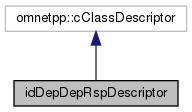
\includegraphics[width=216pt]{classid_dep_dep_rsp_descriptor__inherit__graph}
\end{center}
\end{figure}


Collaboration diagram for id\+Dep\+Dep\+Rsp\+Descriptor\+:
\nopagebreak
\begin{figure}[H]
\begin{center}
\leavevmode
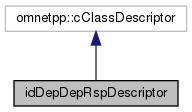
\includegraphics[width=216pt]{classid_dep_dep_rsp_descriptor__coll__graph}
\end{center}
\end{figure}
\subsection*{Public Member Functions}
\begin{DoxyCompactItemize}
\item 
\hyperlink{classid_dep_dep_rsp_descriptor_a3e2274676a0c9a331848c609c9896ecf}{id\+Dep\+Dep\+Rsp\+Descriptor} ()
\item 
virtual \hyperlink{classid_dep_dep_rsp_descriptor_a35bc747b5221c962f04af7f5370f7f4b}{$\sim$id\+Dep\+Dep\+Rsp\+Descriptor} ()
\item 
virtual bool \hyperlink{classid_dep_dep_rsp_descriptor_a67b0832686fbd38cfb80742967116e83}{does\+Support} (omnetpp\+::c\+Object $\ast$obj) const override
\item 
virtual const char $\ast$$\ast$ \hyperlink{classid_dep_dep_rsp_descriptor_a1d0ba88794577cd83f8d752bbf61845b}{get\+Property\+Names} () const override
\item 
virtual const char $\ast$ \hyperlink{classid_dep_dep_rsp_descriptor_ad149f4ccae414eb97ce9959fe4b852c7}{get\+Property} (const char $\ast$propertyname) const override
\item 
virtual int \hyperlink{classid_dep_dep_rsp_descriptor_a7dcb46ff173cfd041ed0299eeef3e09d}{get\+Field\+Count} () const override
\item 
virtual const char $\ast$ \hyperlink{classid_dep_dep_rsp_descriptor_a74aea0c9020a73de0a76814586b94406}{get\+Field\+Name} (int field) const override
\item 
virtual int \hyperlink{classid_dep_dep_rsp_descriptor_ae74524f33495bc3f07c716c8f8ca2d1f}{find\+Field} (const char $\ast$field\+Name) const override
\item 
virtual unsigned int \hyperlink{classid_dep_dep_rsp_descriptor_a93352aea8757f59f6ae4f349733a4dea}{get\+Field\+Type\+Flags} (int field) const override
\item 
virtual const char $\ast$ \hyperlink{classid_dep_dep_rsp_descriptor_af3d0017c6dfbd3fceb127ea34563d7fe}{get\+Field\+Type\+String} (int field) const override
\item 
virtual const char $\ast$$\ast$ \hyperlink{classid_dep_dep_rsp_descriptor_aa14ccdc15e3d4c79f0ae6517d1222e8f}{get\+Field\+Property\+Names} (int field) const override
\item 
virtual const char $\ast$ \hyperlink{classid_dep_dep_rsp_descriptor_a177024add048c4071ea703c072a2733c}{get\+Field\+Property} (int field, const char $\ast$propertyname) const override
\item 
virtual int \hyperlink{classid_dep_dep_rsp_descriptor_ac8e4e19a337c5833273ca1da6488a05d}{get\+Field\+Array\+Size} (void $\ast$object, int field) const override
\item 
virtual const char $\ast$ \hyperlink{classid_dep_dep_rsp_descriptor_a21fe7bc28bb91b7f5d8ce9d84ba1c755}{get\+Field\+Dynamic\+Type\+String} (void $\ast$object, int field, int i) const override
\item 
virtual std\+::string \hyperlink{classid_dep_dep_rsp_descriptor_a3f78b6586d3e0239bf8a530398d6db8c}{get\+Field\+Value\+As\+String} (void $\ast$object, int field, int i) const override
\item 
virtual bool \hyperlink{classid_dep_dep_rsp_descriptor_a03ed926bf151d7c66ac1e6c659013664}{set\+Field\+Value\+As\+String} (void $\ast$object, int field, int i, const char $\ast$value) const override
\item 
virtual const char $\ast$ \hyperlink{classid_dep_dep_rsp_descriptor_ae19bb4da10ef518d7708e9022cc82cca}{get\+Field\+Struct\+Name} (int field) const override
\item 
virtual void $\ast$ \hyperlink{classid_dep_dep_rsp_descriptor_a93338cef2d20630f79cf1f93a081016b}{get\+Field\+Struct\+Value\+Pointer} (void $\ast$object, int field, int i) const override
\end{DoxyCompactItemize}
\subsection*{Private Attributes}
\begin{DoxyCompactItemize}
\item 
const char $\ast$$\ast$ \hyperlink{classid_dep_dep_rsp_descriptor_ab0e20b196152a98a783f887a12b06ff9}{propertynames}
\end{DoxyCompactItemize}


\subsection{Constructor \& Destructor Documentation}
\mbox{\Hypertarget{classid_dep_dep_rsp_descriptor_a3e2274676a0c9a331848c609c9896ecf}\label{classid_dep_dep_rsp_descriptor_a3e2274676a0c9a331848c609c9896ecf}} 
\index{id\+Dep\+Dep\+Rsp\+Descriptor@{id\+Dep\+Dep\+Rsp\+Descriptor}!id\+Dep\+Dep\+Rsp\+Descriptor@{id\+Dep\+Dep\+Rsp\+Descriptor}}
\index{id\+Dep\+Dep\+Rsp\+Descriptor@{id\+Dep\+Dep\+Rsp\+Descriptor}!id\+Dep\+Dep\+Rsp\+Descriptor@{id\+Dep\+Dep\+Rsp\+Descriptor}}
\subsubsection{\texorpdfstring{id\+Dep\+Dep\+Rsp\+Descriptor()}{idDepDepRspDescriptor()}}
{\footnotesize\ttfamily id\+Dep\+Dep\+Rsp\+Descriptor\+::id\+Dep\+Dep\+Rsp\+Descriptor (\begin{DoxyParamCaption}{ }\end{DoxyParamCaption})}

\mbox{\Hypertarget{classid_dep_dep_rsp_descriptor_a35bc747b5221c962f04af7f5370f7f4b}\label{classid_dep_dep_rsp_descriptor_a35bc747b5221c962f04af7f5370f7f4b}} 
\index{id\+Dep\+Dep\+Rsp\+Descriptor@{id\+Dep\+Dep\+Rsp\+Descriptor}!````~id\+Dep\+Dep\+Rsp\+Descriptor@{$\sim$id\+Dep\+Dep\+Rsp\+Descriptor}}
\index{````~id\+Dep\+Dep\+Rsp\+Descriptor@{$\sim$id\+Dep\+Dep\+Rsp\+Descriptor}!id\+Dep\+Dep\+Rsp\+Descriptor@{id\+Dep\+Dep\+Rsp\+Descriptor}}
\subsubsection{\texorpdfstring{$\sim$id\+Dep\+Dep\+Rsp\+Descriptor()}{~idDepDepRspDescriptor()}}
{\footnotesize\ttfamily id\+Dep\+Dep\+Rsp\+Descriptor\+::$\sim$id\+Dep\+Dep\+Rsp\+Descriptor (\begin{DoxyParamCaption}{ }\end{DoxyParamCaption})\hspace{0.3cm}{\ttfamily [virtual]}}



\subsection{Member Function Documentation}
\mbox{\Hypertarget{classid_dep_dep_rsp_descriptor_a67b0832686fbd38cfb80742967116e83}\label{classid_dep_dep_rsp_descriptor_a67b0832686fbd38cfb80742967116e83}} 
\index{id\+Dep\+Dep\+Rsp\+Descriptor@{id\+Dep\+Dep\+Rsp\+Descriptor}!does\+Support@{does\+Support}}
\index{does\+Support@{does\+Support}!id\+Dep\+Dep\+Rsp\+Descriptor@{id\+Dep\+Dep\+Rsp\+Descriptor}}
\subsubsection{\texorpdfstring{does\+Support()}{doesSupport()}}
{\footnotesize\ttfamily bool id\+Dep\+Dep\+Rsp\+Descriptor\+::does\+Support (\begin{DoxyParamCaption}\item[{omnetpp\+::c\+Object $\ast$}]{obj }\end{DoxyParamCaption}) const\hspace{0.3cm}{\ttfamily [override]}, {\ttfamily [virtual]}}

\mbox{\Hypertarget{classid_dep_dep_rsp_descriptor_ae74524f33495bc3f07c716c8f8ca2d1f}\label{classid_dep_dep_rsp_descriptor_ae74524f33495bc3f07c716c8f8ca2d1f}} 
\index{id\+Dep\+Dep\+Rsp\+Descriptor@{id\+Dep\+Dep\+Rsp\+Descriptor}!find\+Field@{find\+Field}}
\index{find\+Field@{find\+Field}!id\+Dep\+Dep\+Rsp\+Descriptor@{id\+Dep\+Dep\+Rsp\+Descriptor}}
\subsubsection{\texorpdfstring{find\+Field()}{findField()}}
{\footnotesize\ttfamily int id\+Dep\+Dep\+Rsp\+Descriptor\+::find\+Field (\begin{DoxyParamCaption}\item[{const char $\ast$}]{field\+Name }\end{DoxyParamCaption}) const\hspace{0.3cm}{\ttfamily [override]}, {\ttfamily [virtual]}}

\mbox{\Hypertarget{classid_dep_dep_rsp_descriptor_ac8e4e19a337c5833273ca1da6488a05d}\label{classid_dep_dep_rsp_descriptor_ac8e4e19a337c5833273ca1da6488a05d}} 
\index{id\+Dep\+Dep\+Rsp\+Descriptor@{id\+Dep\+Dep\+Rsp\+Descriptor}!get\+Field\+Array\+Size@{get\+Field\+Array\+Size}}
\index{get\+Field\+Array\+Size@{get\+Field\+Array\+Size}!id\+Dep\+Dep\+Rsp\+Descriptor@{id\+Dep\+Dep\+Rsp\+Descriptor}}
\subsubsection{\texorpdfstring{get\+Field\+Array\+Size()}{getFieldArraySize()}}
{\footnotesize\ttfamily int id\+Dep\+Dep\+Rsp\+Descriptor\+::get\+Field\+Array\+Size (\begin{DoxyParamCaption}\item[{void $\ast$}]{object,  }\item[{int}]{field }\end{DoxyParamCaption}) const\hspace{0.3cm}{\ttfamily [override]}, {\ttfamily [virtual]}}

\mbox{\Hypertarget{classid_dep_dep_rsp_descriptor_a7dcb46ff173cfd041ed0299eeef3e09d}\label{classid_dep_dep_rsp_descriptor_a7dcb46ff173cfd041ed0299eeef3e09d}} 
\index{id\+Dep\+Dep\+Rsp\+Descriptor@{id\+Dep\+Dep\+Rsp\+Descriptor}!get\+Field\+Count@{get\+Field\+Count}}
\index{get\+Field\+Count@{get\+Field\+Count}!id\+Dep\+Dep\+Rsp\+Descriptor@{id\+Dep\+Dep\+Rsp\+Descriptor}}
\subsubsection{\texorpdfstring{get\+Field\+Count()}{getFieldCount()}}
{\footnotesize\ttfamily int id\+Dep\+Dep\+Rsp\+Descriptor\+::get\+Field\+Count (\begin{DoxyParamCaption}{ }\end{DoxyParamCaption}) const\hspace{0.3cm}{\ttfamily [override]}, {\ttfamily [virtual]}}

\mbox{\Hypertarget{classid_dep_dep_rsp_descriptor_a21fe7bc28bb91b7f5d8ce9d84ba1c755}\label{classid_dep_dep_rsp_descriptor_a21fe7bc28bb91b7f5d8ce9d84ba1c755}} 
\index{id\+Dep\+Dep\+Rsp\+Descriptor@{id\+Dep\+Dep\+Rsp\+Descriptor}!get\+Field\+Dynamic\+Type\+String@{get\+Field\+Dynamic\+Type\+String}}
\index{get\+Field\+Dynamic\+Type\+String@{get\+Field\+Dynamic\+Type\+String}!id\+Dep\+Dep\+Rsp\+Descriptor@{id\+Dep\+Dep\+Rsp\+Descriptor}}
\subsubsection{\texorpdfstring{get\+Field\+Dynamic\+Type\+String()}{getFieldDynamicTypeString()}}
{\footnotesize\ttfamily const char $\ast$ id\+Dep\+Dep\+Rsp\+Descriptor\+::get\+Field\+Dynamic\+Type\+String (\begin{DoxyParamCaption}\item[{void $\ast$}]{object,  }\item[{int}]{field,  }\item[{int}]{i }\end{DoxyParamCaption}) const\hspace{0.3cm}{\ttfamily [override]}, {\ttfamily [virtual]}}

\mbox{\Hypertarget{classid_dep_dep_rsp_descriptor_a74aea0c9020a73de0a76814586b94406}\label{classid_dep_dep_rsp_descriptor_a74aea0c9020a73de0a76814586b94406}} 
\index{id\+Dep\+Dep\+Rsp\+Descriptor@{id\+Dep\+Dep\+Rsp\+Descriptor}!get\+Field\+Name@{get\+Field\+Name}}
\index{get\+Field\+Name@{get\+Field\+Name}!id\+Dep\+Dep\+Rsp\+Descriptor@{id\+Dep\+Dep\+Rsp\+Descriptor}}
\subsubsection{\texorpdfstring{get\+Field\+Name()}{getFieldName()}}
{\footnotesize\ttfamily const char $\ast$ id\+Dep\+Dep\+Rsp\+Descriptor\+::get\+Field\+Name (\begin{DoxyParamCaption}\item[{int}]{field }\end{DoxyParamCaption}) const\hspace{0.3cm}{\ttfamily [override]}, {\ttfamily [virtual]}}

\mbox{\Hypertarget{classid_dep_dep_rsp_descriptor_a177024add048c4071ea703c072a2733c}\label{classid_dep_dep_rsp_descriptor_a177024add048c4071ea703c072a2733c}} 
\index{id\+Dep\+Dep\+Rsp\+Descriptor@{id\+Dep\+Dep\+Rsp\+Descriptor}!get\+Field\+Property@{get\+Field\+Property}}
\index{get\+Field\+Property@{get\+Field\+Property}!id\+Dep\+Dep\+Rsp\+Descriptor@{id\+Dep\+Dep\+Rsp\+Descriptor}}
\subsubsection{\texorpdfstring{get\+Field\+Property()}{getFieldProperty()}}
{\footnotesize\ttfamily const char $\ast$ id\+Dep\+Dep\+Rsp\+Descriptor\+::get\+Field\+Property (\begin{DoxyParamCaption}\item[{int}]{field,  }\item[{const char $\ast$}]{propertyname }\end{DoxyParamCaption}) const\hspace{0.3cm}{\ttfamily [override]}, {\ttfamily [virtual]}}

\mbox{\Hypertarget{classid_dep_dep_rsp_descriptor_aa14ccdc15e3d4c79f0ae6517d1222e8f}\label{classid_dep_dep_rsp_descriptor_aa14ccdc15e3d4c79f0ae6517d1222e8f}} 
\index{id\+Dep\+Dep\+Rsp\+Descriptor@{id\+Dep\+Dep\+Rsp\+Descriptor}!get\+Field\+Property\+Names@{get\+Field\+Property\+Names}}
\index{get\+Field\+Property\+Names@{get\+Field\+Property\+Names}!id\+Dep\+Dep\+Rsp\+Descriptor@{id\+Dep\+Dep\+Rsp\+Descriptor}}
\subsubsection{\texorpdfstring{get\+Field\+Property\+Names()}{getFieldPropertyNames()}}
{\footnotesize\ttfamily const char $\ast$$\ast$ id\+Dep\+Dep\+Rsp\+Descriptor\+::get\+Field\+Property\+Names (\begin{DoxyParamCaption}\item[{int}]{field }\end{DoxyParamCaption}) const\hspace{0.3cm}{\ttfamily [override]}, {\ttfamily [virtual]}}

\mbox{\Hypertarget{classid_dep_dep_rsp_descriptor_ae19bb4da10ef518d7708e9022cc82cca}\label{classid_dep_dep_rsp_descriptor_ae19bb4da10ef518d7708e9022cc82cca}} 
\index{id\+Dep\+Dep\+Rsp\+Descriptor@{id\+Dep\+Dep\+Rsp\+Descriptor}!get\+Field\+Struct\+Name@{get\+Field\+Struct\+Name}}
\index{get\+Field\+Struct\+Name@{get\+Field\+Struct\+Name}!id\+Dep\+Dep\+Rsp\+Descriptor@{id\+Dep\+Dep\+Rsp\+Descriptor}}
\subsubsection{\texorpdfstring{get\+Field\+Struct\+Name()}{getFieldStructName()}}
{\footnotesize\ttfamily const char $\ast$ id\+Dep\+Dep\+Rsp\+Descriptor\+::get\+Field\+Struct\+Name (\begin{DoxyParamCaption}\item[{int}]{field }\end{DoxyParamCaption}) const\hspace{0.3cm}{\ttfamily [override]}, {\ttfamily [virtual]}}

\mbox{\Hypertarget{classid_dep_dep_rsp_descriptor_a93338cef2d20630f79cf1f93a081016b}\label{classid_dep_dep_rsp_descriptor_a93338cef2d20630f79cf1f93a081016b}} 
\index{id\+Dep\+Dep\+Rsp\+Descriptor@{id\+Dep\+Dep\+Rsp\+Descriptor}!get\+Field\+Struct\+Value\+Pointer@{get\+Field\+Struct\+Value\+Pointer}}
\index{get\+Field\+Struct\+Value\+Pointer@{get\+Field\+Struct\+Value\+Pointer}!id\+Dep\+Dep\+Rsp\+Descriptor@{id\+Dep\+Dep\+Rsp\+Descriptor}}
\subsubsection{\texorpdfstring{get\+Field\+Struct\+Value\+Pointer()}{getFieldStructValuePointer()}}
{\footnotesize\ttfamily void $\ast$ id\+Dep\+Dep\+Rsp\+Descriptor\+::get\+Field\+Struct\+Value\+Pointer (\begin{DoxyParamCaption}\item[{void $\ast$}]{object,  }\item[{int}]{field,  }\item[{int}]{i }\end{DoxyParamCaption}) const\hspace{0.3cm}{\ttfamily [override]}, {\ttfamily [virtual]}}

\mbox{\Hypertarget{classid_dep_dep_rsp_descriptor_a93352aea8757f59f6ae4f349733a4dea}\label{classid_dep_dep_rsp_descriptor_a93352aea8757f59f6ae4f349733a4dea}} 
\index{id\+Dep\+Dep\+Rsp\+Descriptor@{id\+Dep\+Dep\+Rsp\+Descriptor}!get\+Field\+Type\+Flags@{get\+Field\+Type\+Flags}}
\index{get\+Field\+Type\+Flags@{get\+Field\+Type\+Flags}!id\+Dep\+Dep\+Rsp\+Descriptor@{id\+Dep\+Dep\+Rsp\+Descriptor}}
\subsubsection{\texorpdfstring{get\+Field\+Type\+Flags()}{getFieldTypeFlags()}}
{\footnotesize\ttfamily unsigned int id\+Dep\+Dep\+Rsp\+Descriptor\+::get\+Field\+Type\+Flags (\begin{DoxyParamCaption}\item[{int}]{field }\end{DoxyParamCaption}) const\hspace{0.3cm}{\ttfamily [override]}, {\ttfamily [virtual]}}

\mbox{\Hypertarget{classid_dep_dep_rsp_descriptor_af3d0017c6dfbd3fceb127ea34563d7fe}\label{classid_dep_dep_rsp_descriptor_af3d0017c6dfbd3fceb127ea34563d7fe}} 
\index{id\+Dep\+Dep\+Rsp\+Descriptor@{id\+Dep\+Dep\+Rsp\+Descriptor}!get\+Field\+Type\+String@{get\+Field\+Type\+String}}
\index{get\+Field\+Type\+String@{get\+Field\+Type\+String}!id\+Dep\+Dep\+Rsp\+Descriptor@{id\+Dep\+Dep\+Rsp\+Descriptor}}
\subsubsection{\texorpdfstring{get\+Field\+Type\+String()}{getFieldTypeString()}}
{\footnotesize\ttfamily const char $\ast$ id\+Dep\+Dep\+Rsp\+Descriptor\+::get\+Field\+Type\+String (\begin{DoxyParamCaption}\item[{int}]{field }\end{DoxyParamCaption}) const\hspace{0.3cm}{\ttfamily [override]}, {\ttfamily [virtual]}}

\mbox{\Hypertarget{classid_dep_dep_rsp_descriptor_a3f78b6586d3e0239bf8a530398d6db8c}\label{classid_dep_dep_rsp_descriptor_a3f78b6586d3e0239bf8a530398d6db8c}} 
\index{id\+Dep\+Dep\+Rsp\+Descriptor@{id\+Dep\+Dep\+Rsp\+Descriptor}!get\+Field\+Value\+As\+String@{get\+Field\+Value\+As\+String}}
\index{get\+Field\+Value\+As\+String@{get\+Field\+Value\+As\+String}!id\+Dep\+Dep\+Rsp\+Descriptor@{id\+Dep\+Dep\+Rsp\+Descriptor}}
\subsubsection{\texorpdfstring{get\+Field\+Value\+As\+String()}{getFieldValueAsString()}}
{\footnotesize\ttfamily std\+::string id\+Dep\+Dep\+Rsp\+Descriptor\+::get\+Field\+Value\+As\+String (\begin{DoxyParamCaption}\item[{void $\ast$}]{object,  }\item[{int}]{field,  }\item[{int}]{i }\end{DoxyParamCaption}) const\hspace{0.3cm}{\ttfamily [override]}, {\ttfamily [virtual]}}

\mbox{\Hypertarget{classid_dep_dep_rsp_descriptor_ad149f4ccae414eb97ce9959fe4b852c7}\label{classid_dep_dep_rsp_descriptor_ad149f4ccae414eb97ce9959fe4b852c7}} 
\index{id\+Dep\+Dep\+Rsp\+Descriptor@{id\+Dep\+Dep\+Rsp\+Descriptor}!get\+Property@{get\+Property}}
\index{get\+Property@{get\+Property}!id\+Dep\+Dep\+Rsp\+Descriptor@{id\+Dep\+Dep\+Rsp\+Descriptor}}
\subsubsection{\texorpdfstring{get\+Property()}{getProperty()}}
{\footnotesize\ttfamily const char $\ast$ id\+Dep\+Dep\+Rsp\+Descriptor\+::get\+Property (\begin{DoxyParamCaption}\item[{const char $\ast$}]{propertyname }\end{DoxyParamCaption}) const\hspace{0.3cm}{\ttfamily [override]}, {\ttfamily [virtual]}}

\mbox{\Hypertarget{classid_dep_dep_rsp_descriptor_a1d0ba88794577cd83f8d752bbf61845b}\label{classid_dep_dep_rsp_descriptor_a1d0ba88794577cd83f8d752bbf61845b}} 
\index{id\+Dep\+Dep\+Rsp\+Descriptor@{id\+Dep\+Dep\+Rsp\+Descriptor}!get\+Property\+Names@{get\+Property\+Names}}
\index{get\+Property\+Names@{get\+Property\+Names}!id\+Dep\+Dep\+Rsp\+Descriptor@{id\+Dep\+Dep\+Rsp\+Descriptor}}
\subsubsection{\texorpdfstring{get\+Property\+Names()}{getPropertyNames()}}
{\footnotesize\ttfamily const char $\ast$$\ast$ id\+Dep\+Dep\+Rsp\+Descriptor\+::get\+Property\+Names (\begin{DoxyParamCaption}{ }\end{DoxyParamCaption}) const\hspace{0.3cm}{\ttfamily [override]}, {\ttfamily [virtual]}}

\mbox{\Hypertarget{classid_dep_dep_rsp_descriptor_a03ed926bf151d7c66ac1e6c659013664}\label{classid_dep_dep_rsp_descriptor_a03ed926bf151d7c66ac1e6c659013664}} 
\index{id\+Dep\+Dep\+Rsp\+Descriptor@{id\+Dep\+Dep\+Rsp\+Descriptor}!set\+Field\+Value\+As\+String@{set\+Field\+Value\+As\+String}}
\index{set\+Field\+Value\+As\+String@{set\+Field\+Value\+As\+String}!id\+Dep\+Dep\+Rsp\+Descriptor@{id\+Dep\+Dep\+Rsp\+Descriptor}}
\subsubsection{\texorpdfstring{set\+Field\+Value\+As\+String()}{setFieldValueAsString()}}
{\footnotesize\ttfamily bool id\+Dep\+Dep\+Rsp\+Descriptor\+::set\+Field\+Value\+As\+String (\begin{DoxyParamCaption}\item[{void $\ast$}]{object,  }\item[{int}]{field,  }\item[{int}]{i,  }\item[{const char $\ast$}]{value }\end{DoxyParamCaption}) const\hspace{0.3cm}{\ttfamily [override]}, {\ttfamily [virtual]}}



\subsection{Member Data Documentation}
\mbox{\Hypertarget{classid_dep_dep_rsp_descriptor_ab0e20b196152a98a783f887a12b06ff9}\label{classid_dep_dep_rsp_descriptor_ab0e20b196152a98a783f887a12b06ff9}} 
\index{id\+Dep\+Dep\+Rsp\+Descriptor@{id\+Dep\+Dep\+Rsp\+Descriptor}!propertynames@{propertynames}}
\index{propertynames@{propertynames}!id\+Dep\+Dep\+Rsp\+Descriptor@{id\+Dep\+Dep\+Rsp\+Descriptor}}
\subsubsection{\texorpdfstring{propertynames}{propertynames}}
{\footnotesize\ttfamily const char$\ast$$\ast$ id\+Dep\+Dep\+Rsp\+Descriptor\+::propertynames\hspace{0.3cm}{\ttfamily [mutable]}, {\ttfamily [private]}}



The documentation for this class was generated from the following file\+:\begin{DoxyCompactItemize}
\item 
/home/wilhelm/\+Documents/code\+Git\+Hub/\+Error\+Detectors/src/\+Messages/\hyperlink{dep_rsp__m_8cc}{dep\+Rsp\+\_\+m.\+cc}\end{DoxyCompactItemize}

\hypertarget{classid_msg_app_msg_descriptor}{}\section{id\+Msg\+App\+Msg\+Descriptor Class Reference}
\label{classid_msg_app_msg_descriptor}\index{id\+Msg\+App\+Msg\+Descriptor@{id\+Msg\+App\+Msg\+Descriptor}}


Inheritance diagram for id\+Msg\+App\+Msg\+Descriptor\+:\nopagebreak
\begin{figure}[H]
\begin{center}
\leavevmode
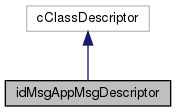
\includegraphics[width=204pt]{classid_msg_app_msg_descriptor__inherit__graph}
\end{center}
\end{figure}


Collaboration diagram for id\+Msg\+App\+Msg\+Descriptor\+:\nopagebreak
\begin{figure}[H]
\begin{center}
\leavevmode
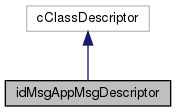
\includegraphics[width=204pt]{classid_msg_app_msg_descriptor__coll__graph}
\end{center}
\end{figure}
\subsection*{Public Member Functions}
\begin{DoxyCompactItemize}
\item 
\hyperlink{classid_msg_app_msg_descriptor_a1f471f84ba71baffc0c0bedf29ff5522}{id\+Msg\+App\+Msg\+Descriptor} ()
\item 
virtual \hyperlink{classid_msg_app_msg_descriptor_a89b66128f3a50e738add1045dbb0e9b2}{$\sim$id\+Msg\+App\+Msg\+Descriptor} ()
\item 
virtual bool \hyperlink{classid_msg_app_msg_descriptor_ace75e5fffbe04839660617b19145128f}{does\+Support} (omnetpp\+::c\+Object $\ast$obj) const override
\item 
virtual const char $\ast$$\ast$ \hyperlink{classid_msg_app_msg_descriptor_a5da6527d679103a0cac6143a160813a7}{get\+Property\+Names} () const override
\item 
virtual const char $\ast$ \hyperlink{classid_msg_app_msg_descriptor_ac9b9240ff817b217015861a922206080}{get\+Property} (const char $\ast$propertyname) const override
\item 
virtual int \hyperlink{classid_msg_app_msg_descriptor_ae8280283eb1f21ecfa541b6e824d8008}{get\+Field\+Count} () const override
\item 
virtual const char $\ast$ \hyperlink{classid_msg_app_msg_descriptor_abc0d2c99d328bee5785de2d5df2a40e3}{get\+Field\+Name} (int field) const override
\item 
virtual int \hyperlink{classid_msg_app_msg_descriptor_a4b04258cc21a7b0c95fbb68719ac489d}{find\+Field} (const char $\ast$field\+Name) const override
\item 
virtual unsigned int \hyperlink{classid_msg_app_msg_descriptor_a9211adf741e2d9bb31f47d210297438e}{get\+Field\+Type\+Flags} (int field) const override
\item 
virtual const char $\ast$ \hyperlink{classid_msg_app_msg_descriptor_a0c976a9e1df2844d8e0897bf0eee8d5a}{get\+Field\+Type\+String} (int field) const override
\item 
virtual const char $\ast$$\ast$ \hyperlink{classid_msg_app_msg_descriptor_a55640ce6067dd59f8fc22cb8c3ce2f29}{get\+Field\+Property\+Names} (int field) const override
\item 
virtual const char $\ast$ \hyperlink{classid_msg_app_msg_descriptor_a69e69da2c64669ba7d0865a63e273e92}{get\+Field\+Property} (int field, const char $\ast$propertyname) const override
\item 
virtual int \hyperlink{classid_msg_app_msg_descriptor_a55b2f838a298f91b5a0ca06fab71bcad}{get\+Field\+Array\+Size} (void $\ast$object, int field) const override
\item 
virtual const char $\ast$ \hyperlink{classid_msg_app_msg_descriptor_a166e1858ebf5b4c0115b540601799992}{get\+Field\+Dynamic\+Type\+String} (void $\ast$object, int field, int i) const override
\item 
virtual std\+::string \hyperlink{classid_msg_app_msg_descriptor_a42e71d687276c6b4ffd5d812eb9216a3}{get\+Field\+Value\+As\+String} (void $\ast$object, int field, int i) const override
\item 
virtual bool \hyperlink{classid_msg_app_msg_descriptor_a6293893d265e9968a97f9226dac829e9}{set\+Field\+Value\+As\+String} (void $\ast$object, int field, int i, const char $\ast$value) const override
\item 
virtual const char $\ast$ \hyperlink{classid_msg_app_msg_descriptor_ab4329d8695157a2583bf560578eca364}{get\+Field\+Struct\+Name} (int field) const override
\item 
virtual void $\ast$ \hyperlink{classid_msg_app_msg_descriptor_a8453c0ef000997f88024f1be37f1e5be}{get\+Field\+Struct\+Value\+Pointer} (void $\ast$object, int field, int i) const override
\end{DoxyCompactItemize}
\subsection*{Private Attributes}
\begin{DoxyCompactItemize}
\item 
const char $\ast$$\ast$ \hyperlink{classid_msg_app_msg_descriptor_a0415274a6b02ab2bd2a2c3226a9b4543}{propertynames}
\end{DoxyCompactItemize}


\subsection{Constructor \& Destructor Documentation}
\mbox{\Hypertarget{classid_msg_app_msg_descriptor_a1f471f84ba71baffc0c0bedf29ff5522}\label{classid_msg_app_msg_descriptor_a1f471f84ba71baffc0c0bedf29ff5522}} 
\index{id\+Msg\+App\+Msg\+Descriptor@{id\+Msg\+App\+Msg\+Descriptor}!id\+Msg\+App\+Msg\+Descriptor@{id\+Msg\+App\+Msg\+Descriptor}}
\index{id\+Msg\+App\+Msg\+Descriptor@{id\+Msg\+App\+Msg\+Descriptor}!id\+Msg\+App\+Msg\+Descriptor@{id\+Msg\+App\+Msg\+Descriptor}}
\subsubsection{\texorpdfstring{id\+Msg\+App\+Msg\+Descriptor()}{idMsgAppMsgDescriptor()}}
{\footnotesize\ttfamily id\+Msg\+App\+Msg\+Descriptor\+::id\+Msg\+App\+Msg\+Descriptor (\begin{DoxyParamCaption}{ }\end{DoxyParamCaption})}

\mbox{\Hypertarget{classid_msg_app_msg_descriptor_a89b66128f3a50e738add1045dbb0e9b2}\label{classid_msg_app_msg_descriptor_a89b66128f3a50e738add1045dbb0e9b2}} 
\index{id\+Msg\+App\+Msg\+Descriptor@{id\+Msg\+App\+Msg\+Descriptor}!````~id\+Msg\+App\+Msg\+Descriptor@{$\sim$id\+Msg\+App\+Msg\+Descriptor}}
\index{````~id\+Msg\+App\+Msg\+Descriptor@{$\sim$id\+Msg\+App\+Msg\+Descriptor}!id\+Msg\+App\+Msg\+Descriptor@{id\+Msg\+App\+Msg\+Descriptor}}
\subsubsection{\texorpdfstring{$\sim$id\+Msg\+App\+Msg\+Descriptor()}{~idMsgAppMsgDescriptor()}}
{\footnotesize\ttfamily id\+Msg\+App\+Msg\+Descriptor\+::$\sim$id\+Msg\+App\+Msg\+Descriptor (\begin{DoxyParamCaption}{ }\end{DoxyParamCaption})\hspace{0.3cm}{\ttfamily [virtual]}}



\subsection{Member Function Documentation}
\mbox{\Hypertarget{classid_msg_app_msg_descriptor_ace75e5fffbe04839660617b19145128f}\label{classid_msg_app_msg_descriptor_ace75e5fffbe04839660617b19145128f}} 
\index{id\+Msg\+App\+Msg\+Descriptor@{id\+Msg\+App\+Msg\+Descriptor}!does\+Support@{does\+Support}}
\index{does\+Support@{does\+Support}!id\+Msg\+App\+Msg\+Descriptor@{id\+Msg\+App\+Msg\+Descriptor}}
\subsubsection{\texorpdfstring{does\+Support()}{doesSupport()}}
{\footnotesize\ttfamily bool id\+Msg\+App\+Msg\+Descriptor\+::does\+Support (\begin{DoxyParamCaption}\item[{omnetpp\+::c\+Object $\ast$}]{obj }\end{DoxyParamCaption}) const\hspace{0.3cm}{\ttfamily [override]}, {\ttfamily [virtual]}}

\mbox{\Hypertarget{classid_msg_app_msg_descriptor_a4b04258cc21a7b0c95fbb68719ac489d}\label{classid_msg_app_msg_descriptor_a4b04258cc21a7b0c95fbb68719ac489d}} 
\index{id\+Msg\+App\+Msg\+Descriptor@{id\+Msg\+App\+Msg\+Descriptor}!find\+Field@{find\+Field}}
\index{find\+Field@{find\+Field}!id\+Msg\+App\+Msg\+Descriptor@{id\+Msg\+App\+Msg\+Descriptor}}
\subsubsection{\texorpdfstring{find\+Field()}{findField()}}
{\footnotesize\ttfamily int id\+Msg\+App\+Msg\+Descriptor\+::find\+Field (\begin{DoxyParamCaption}\item[{const char $\ast$}]{field\+Name }\end{DoxyParamCaption}) const\hspace{0.3cm}{\ttfamily [override]}, {\ttfamily [virtual]}}

\mbox{\Hypertarget{classid_msg_app_msg_descriptor_a55b2f838a298f91b5a0ca06fab71bcad}\label{classid_msg_app_msg_descriptor_a55b2f838a298f91b5a0ca06fab71bcad}} 
\index{id\+Msg\+App\+Msg\+Descriptor@{id\+Msg\+App\+Msg\+Descriptor}!get\+Field\+Array\+Size@{get\+Field\+Array\+Size}}
\index{get\+Field\+Array\+Size@{get\+Field\+Array\+Size}!id\+Msg\+App\+Msg\+Descriptor@{id\+Msg\+App\+Msg\+Descriptor}}
\subsubsection{\texorpdfstring{get\+Field\+Array\+Size()}{getFieldArraySize()}}
{\footnotesize\ttfamily int id\+Msg\+App\+Msg\+Descriptor\+::get\+Field\+Array\+Size (\begin{DoxyParamCaption}\item[{void $\ast$}]{object,  }\item[{int}]{field }\end{DoxyParamCaption}) const\hspace{0.3cm}{\ttfamily [override]}, {\ttfamily [virtual]}}

\mbox{\Hypertarget{classid_msg_app_msg_descriptor_ae8280283eb1f21ecfa541b6e824d8008}\label{classid_msg_app_msg_descriptor_ae8280283eb1f21ecfa541b6e824d8008}} 
\index{id\+Msg\+App\+Msg\+Descriptor@{id\+Msg\+App\+Msg\+Descriptor}!get\+Field\+Count@{get\+Field\+Count}}
\index{get\+Field\+Count@{get\+Field\+Count}!id\+Msg\+App\+Msg\+Descriptor@{id\+Msg\+App\+Msg\+Descriptor}}
\subsubsection{\texorpdfstring{get\+Field\+Count()}{getFieldCount()}}
{\footnotesize\ttfamily int id\+Msg\+App\+Msg\+Descriptor\+::get\+Field\+Count (\begin{DoxyParamCaption}{ }\end{DoxyParamCaption}) const\hspace{0.3cm}{\ttfamily [override]}, {\ttfamily [virtual]}}

\mbox{\Hypertarget{classid_msg_app_msg_descriptor_a166e1858ebf5b4c0115b540601799992}\label{classid_msg_app_msg_descriptor_a166e1858ebf5b4c0115b540601799992}} 
\index{id\+Msg\+App\+Msg\+Descriptor@{id\+Msg\+App\+Msg\+Descriptor}!get\+Field\+Dynamic\+Type\+String@{get\+Field\+Dynamic\+Type\+String}}
\index{get\+Field\+Dynamic\+Type\+String@{get\+Field\+Dynamic\+Type\+String}!id\+Msg\+App\+Msg\+Descriptor@{id\+Msg\+App\+Msg\+Descriptor}}
\subsubsection{\texorpdfstring{get\+Field\+Dynamic\+Type\+String()}{getFieldDynamicTypeString()}}
{\footnotesize\ttfamily const char $\ast$ id\+Msg\+App\+Msg\+Descriptor\+::get\+Field\+Dynamic\+Type\+String (\begin{DoxyParamCaption}\item[{void $\ast$}]{object,  }\item[{int}]{field,  }\item[{int}]{i }\end{DoxyParamCaption}) const\hspace{0.3cm}{\ttfamily [override]}, {\ttfamily [virtual]}}

\mbox{\Hypertarget{classid_msg_app_msg_descriptor_abc0d2c99d328bee5785de2d5df2a40e3}\label{classid_msg_app_msg_descriptor_abc0d2c99d328bee5785de2d5df2a40e3}} 
\index{id\+Msg\+App\+Msg\+Descriptor@{id\+Msg\+App\+Msg\+Descriptor}!get\+Field\+Name@{get\+Field\+Name}}
\index{get\+Field\+Name@{get\+Field\+Name}!id\+Msg\+App\+Msg\+Descriptor@{id\+Msg\+App\+Msg\+Descriptor}}
\subsubsection{\texorpdfstring{get\+Field\+Name()}{getFieldName()}}
{\footnotesize\ttfamily const char $\ast$ id\+Msg\+App\+Msg\+Descriptor\+::get\+Field\+Name (\begin{DoxyParamCaption}\item[{int}]{field }\end{DoxyParamCaption}) const\hspace{0.3cm}{\ttfamily [override]}, {\ttfamily [virtual]}}

\mbox{\Hypertarget{classid_msg_app_msg_descriptor_a69e69da2c64669ba7d0865a63e273e92}\label{classid_msg_app_msg_descriptor_a69e69da2c64669ba7d0865a63e273e92}} 
\index{id\+Msg\+App\+Msg\+Descriptor@{id\+Msg\+App\+Msg\+Descriptor}!get\+Field\+Property@{get\+Field\+Property}}
\index{get\+Field\+Property@{get\+Field\+Property}!id\+Msg\+App\+Msg\+Descriptor@{id\+Msg\+App\+Msg\+Descriptor}}
\subsubsection{\texorpdfstring{get\+Field\+Property()}{getFieldProperty()}}
{\footnotesize\ttfamily const char $\ast$ id\+Msg\+App\+Msg\+Descriptor\+::get\+Field\+Property (\begin{DoxyParamCaption}\item[{int}]{field,  }\item[{const char $\ast$}]{propertyname }\end{DoxyParamCaption}) const\hspace{0.3cm}{\ttfamily [override]}, {\ttfamily [virtual]}}

\mbox{\Hypertarget{classid_msg_app_msg_descriptor_a55640ce6067dd59f8fc22cb8c3ce2f29}\label{classid_msg_app_msg_descriptor_a55640ce6067dd59f8fc22cb8c3ce2f29}} 
\index{id\+Msg\+App\+Msg\+Descriptor@{id\+Msg\+App\+Msg\+Descriptor}!get\+Field\+Property\+Names@{get\+Field\+Property\+Names}}
\index{get\+Field\+Property\+Names@{get\+Field\+Property\+Names}!id\+Msg\+App\+Msg\+Descriptor@{id\+Msg\+App\+Msg\+Descriptor}}
\subsubsection{\texorpdfstring{get\+Field\+Property\+Names()}{getFieldPropertyNames()}}
{\footnotesize\ttfamily const char $\ast$$\ast$ id\+Msg\+App\+Msg\+Descriptor\+::get\+Field\+Property\+Names (\begin{DoxyParamCaption}\item[{int}]{field }\end{DoxyParamCaption}) const\hspace{0.3cm}{\ttfamily [override]}, {\ttfamily [virtual]}}

\mbox{\Hypertarget{classid_msg_app_msg_descriptor_ab4329d8695157a2583bf560578eca364}\label{classid_msg_app_msg_descriptor_ab4329d8695157a2583bf560578eca364}} 
\index{id\+Msg\+App\+Msg\+Descriptor@{id\+Msg\+App\+Msg\+Descriptor}!get\+Field\+Struct\+Name@{get\+Field\+Struct\+Name}}
\index{get\+Field\+Struct\+Name@{get\+Field\+Struct\+Name}!id\+Msg\+App\+Msg\+Descriptor@{id\+Msg\+App\+Msg\+Descriptor}}
\subsubsection{\texorpdfstring{get\+Field\+Struct\+Name()}{getFieldStructName()}}
{\footnotesize\ttfamily const char $\ast$ id\+Msg\+App\+Msg\+Descriptor\+::get\+Field\+Struct\+Name (\begin{DoxyParamCaption}\item[{int}]{field }\end{DoxyParamCaption}) const\hspace{0.3cm}{\ttfamily [override]}, {\ttfamily [virtual]}}

\mbox{\Hypertarget{classid_msg_app_msg_descriptor_a8453c0ef000997f88024f1be37f1e5be}\label{classid_msg_app_msg_descriptor_a8453c0ef000997f88024f1be37f1e5be}} 
\index{id\+Msg\+App\+Msg\+Descriptor@{id\+Msg\+App\+Msg\+Descriptor}!get\+Field\+Struct\+Value\+Pointer@{get\+Field\+Struct\+Value\+Pointer}}
\index{get\+Field\+Struct\+Value\+Pointer@{get\+Field\+Struct\+Value\+Pointer}!id\+Msg\+App\+Msg\+Descriptor@{id\+Msg\+App\+Msg\+Descriptor}}
\subsubsection{\texorpdfstring{get\+Field\+Struct\+Value\+Pointer()}{getFieldStructValuePointer()}}
{\footnotesize\ttfamily void $\ast$ id\+Msg\+App\+Msg\+Descriptor\+::get\+Field\+Struct\+Value\+Pointer (\begin{DoxyParamCaption}\item[{void $\ast$}]{object,  }\item[{int}]{field,  }\item[{int}]{i }\end{DoxyParamCaption}) const\hspace{0.3cm}{\ttfamily [override]}, {\ttfamily [virtual]}}

\mbox{\Hypertarget{classid_msg_app_msg_descriptor_a9211adf741e2d9bb31f47d210297438e}\label{classid_msg_app_msg_descriptor_a9211adf741e2d9bb31f47d210297438e}} 
\index{id\+Msg\+App\+Msg\+Descriptor@{id\+Msg\+App\+Msg\+Descriptor}!get\+Field\+Type\+Flags@{get\+Field\+Type\+Flags}}
\index{get\+Field\+Type\+Flags@{get\+Field\+Type\+Flags}!id\+Msg\+App\+Msg\+Descriptor@{id\+Msg\+App\+Msg\+Descriptor}}
\subsubsection{\texorpdfstring{get\+Field\+Type\+Flags()}{getFieldTypeFlags()}}
{\footnotesize\ttfamily unsigned int id\+Msg\+App\+Msg\+Descriptor\+::get\+Field\+Type\+Flags (\begin{DoxyParamCaption}\item[{int}]{field }\end{DoxyParamCaption}) const\hspace{0.3cm}{\ttfamily [override]}, {\ttfamily [virtual]}}

\mbox{\Hypertarget{classid_msg_app_msg_descriptor_a0c976a9e1df2844d8e0897bf0eee8d5a}\label{classid_msg_app_msg_descriptor_a0c976a9e1df2844d8e0897bf0eee8d5a}} 
\index{id\+Msg\+App\+Msg\+Descriptor@{id\+Msg\+App\+Msg\+Descriptor}!get\+Field\+Type\+String@{get\+Field\+Type\+String}}
\index{get\+Field\+Type\+String@{get\+Field\+Type\+String}!id\+Msg\+App\+Msg\+Descriptor@{id\+Msg\+App\+Msg\+Descriptor}}
\subsubsection{\texorpdfstring{get\+Field\+Type\+String()}{getFieldTypeString()}}
{\footnotesize\ttfamily const char $\ast$ id\+Msg\+App\+Msg\+Descriptor\+::get\+Field\+Type\+String (\begin{DoxyParamCaption}\item[{int}]{field }\end{DoxyParamCaption}) const\hspace{0.3cm}{\ttfamily [override]}, {\ttfamily [virtual]}}

\mbox{\Hypertarget{classid_msg_app_msg_descriptor_a42e71d687276c6b4ffd5d812eb9216a3}\label{classid_msg_app_msg_descriptor_a42e71d687276c6b4ffd5d812eb9216a3}} 
\index{id\+Msg\+App\+Msg\+Descriptor@{id\+Msg\+App\+Msg\+Descriptor}!get\+Field\+Value\+As\+String@{get\+Field\+Value\+As\+String}}
\index{get\+Field\+Value\+As\+String@{get\+Field\+Value\+As\+String}!id\+Msg\+App\+Msg\+Descriptor@{id\+Msg\+App\+Msg\+Descriptor}}
\subsubsection{\texorpdfstring{get\+Field\+Value\+As\+String()}{getFieldValueAsString()}}
{\footnotesize\ttfamily std\+::string id\+Msg\+App\+Msg\+Descriptor\+::get\+Field\+Value\+As\+String (\begin{DoxyParamCaption}\item[{void $\ast$}]{object,  }\item[{int}]{field,  }\item[{int}]{i }\end{DoxyParamCaption}) const\hspace{0.3cm}{\ttfamily [override]}, {\ttfamily [virtual]}}

\mbox{\Hypertarget{classid_msg_app_msg_descriptor_ac9b9240ff817b217015861a922206080}\label{classid_msg_app_msg_descriptor_ac9b9240ff817b217015861a922206080}} 
\index{id\+Msg\+App\+Msg\+Descriptor@{id\+Msg\+App\+Msg\+Descriptor}!get\+Property@{get\+Property}}
\index{get\+Property@{get\+Property}!id\+Msg\+App\+Msg\+Descriptor@{id\+Msg\+App\+Msg\+Descriptor}}
\subsubsection{\texorpdfstring{get\+Property()}{getProperty()}}
{\footnotesize\ttfamily const char $\ast$ id\+Msg\+App\+Msg\+Descriptor\+::get\+Property (\begin{DoxyParamCaption}\item[{const char $\ast$}]{propertyname }\end{DoxyParamCaption}) const\hspace{0.3cm}{\ttfamily [override]}, {\ttfamily [virtual]}}

\mbox{\Hypertarget{classid_msg_app_msg_descriptor_a5da6527d679103a0cac6143a160813a7}\label{classid_msg_app_msg_descriptor_a5da6527d679103a0cac6143a160813a7}} 
\index{id\+Msg\+App\+Msg\+Descriptor@{id\+Msg\+App\+Msg\+Descriptor}!get\+Property\+Names@{get\+Property\+Names}}
\index{get\+Property\+Names@{get\+Property\+Names}!id\+Msg\+App\+Msg\+Descriptor@{id\+Msg\+App\+Msg\+Descriptor}}
\subsubsection{\texorpdfstring{get\+Property\+Names()}{getPropertyNames()}}
{\footnotesize\ttfamily const char $\ast$$\ast$ id\+Msg\+App\+Msg\+Descriptor\+::get\+Property\+Names (\begin{DoxyParamCaption}{ }\end{DoxyParamCaption}) const\hspace{0.3cm}{\ttfamily [override]}, {\ttfamily [virtual]}}

\mbox{\Hypertarget{classid_msg_app_msg_descriptor_a6293893d265e9968a97f9226dac829e9}\label{classid_msg_app_msg_descriptor_a6293893d265e9968a97f9226dac829e9}} 
\index{id\+Msg\+App\+Msg\+Descriptor@{id\+Msg\+App\+Msg\+Descriptor}!set\+Field\+Value\+As\+String@{set\+Field\+Value\+As\+String}}
\index{set\+Field\+Value\+As\+String@{set\+Field\+Value\+As\+String}!id\+Msg\+App\+Msg\+Descriptor@{id\+Msg\+App\+Msg\+Descriptor}}
\subsubsection{\texorpdfstring{set\+Field\+Value\+As\+String()}{setFieldValueAsString()}}
{\footnotesize\ttfamily bool id\+Msg\+App\+Msg\+Descriptor\+::set\+Field\+Value\+As\+String (\begin{DoxyParamCaption}\item[{void $\ast$}]{object,  }\item[{int}]{field,  }\item[{int}]{i,  }\item[{const char $\ast$}]{value }\end{DoxyParamCaption}) const\hspace{0.3cm}{\ttfamily [override]}, {\ttfamily [virtual]}}



\subsection{Member Data Documentation}
\mbox{\Hypertarget{classid_msg_app_msg_descriptor_a0415274a6b02ab2bd2a2c3226a9b4543}\label{classid_msg_app_msg_descriptor_a0415274a6b02ab2bd2a2c3226a9b4543}} 
\index{id\+Msg\+App\+Msg\+Descriptor@{id\+Msg\+App\+Msg\+Descriptor}!propertynames@{propertynames}}
\index{propertynames@{propertynames}!id\+Msg\+App\+Msg\+Descriptor@{id\+Msg\+App\+Msg\+Descriptor}}
\subsubsection{\texorpdfstring{propertynames}{propertynames}}
{\footnotesize\ttfamily const char$\ast$$\ast$ id\+Msg\+App\+Msg\+Descriptor\+::propertynames\hspace{0.3cm}{\ttfamily [mutable]}, {\ttfamily [private]}}



The documentation for this class was generated from the following file\+:\begin{DoxyCompactItemize}
\item 
src/\+Messages/\hyperlink{_app_msg__m_8cc}{App\+Msg\+\_\+m.\+cc}\end{DoxyCompactItemize}

\hypertarget{classid_msg_dep_req_descriptor}{}\section{id\+Msg\+Dep\+Req\+Descriptor Class Reference}
\label{classid_msg_dep_req_descriptor}\index{id\+Msg\+Dep\+Req\+Descriptor@{id\+Msg\+Dep\+Req\+Descriptor}}


Inheritance diagram for id\+Msg\+Dep\+Req\+Descriptor\+:\nopagebreak
\begin{figure}[H]
\begin{center}
\leavevmode
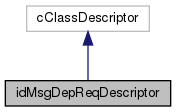
\includegraphics[width=204pt]{classid_msg_dep_req_descriptor__inherit__graph}
\end{center}
\end{figure}


Collaboration diagram for id\+Msg\+Dep\+Req\+Descriptor\+:\nopagebreak
\begin{figure}[H]
\begin{center}
\leavevmode
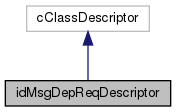
\includegraphics[width=204pt]{classid_msg_dep_req_descriptor__coll__graph}
\end{center}
\end{figure}
\subsection*{Public Member Functions}
\begin{DoxyCompactItemize}
\item 
\hyperlink{classid_msg_dep_req_descriptor_a2f3ef90d3ded0e3218bbd9577c207dfa}{id\+Msg\+Dep\+Req\+Descriptor} ()
\item 
virtual \hyperlink{classid_msg_dep_req_descriptor_aee85d0507fe535a9dd7a5c793d0941ed}{$\sim$id\+Msg\+Dep\+Req\+Descriptor} ()
\item 
virtual bool \hyperlink{classid_msg_dep_req_descriptor_a866862bf6ada354e5f85cdd65c57f394}{does\+Support} (omnetpp\+::c\+Object $\ast$obj) const override
\item 
virtual const char $\ast$$\ast$ \hyperlink{classid_msg_dep_req_descriptor_a7150bb9f317973c98f118ba004de28cc}{get\+Property\+Names} () const override
\item 
virtual const char $\ast$ \hyperlink{classid_msg_dep_req_descriptor_a389f447ccbaba22709ec52b3ed5438f7}{get\+Property} (const char $\ast$propertyname) const override
\item 
virtual int \hyperlink{classid_msg_dep_req_descriptor_a36d7503463f93c4422429b63f94ba12e}{get\+Field\+Count} () const override
\item 
virtual const char $\ast$ \hyperlink{classid_msg_dep_req_descriptor_a7bb154c4ddb6234b3ada7a80e9d92cb8}{get\+Field\+Name} (int field) const override
\item 
virtual int \hyperlink{classid_msg_dep_req_descriptor_afb1d884343c3a15781c749a5d054cd7c}{find\+Field} (const char $\ast$field\+Name) const override
\item 
virtual unsigned int \hyperlink{classid_msg_dep_req_descriptor_acb44b456dc185a621c29b37511e58ae8}{get\+Field\+Type\+Flags} (int field) const override
\item 
virtual const char $\ast$ \hyperlink{classid_msg_dep_req_descriptor_aadee504ad5a0a6d979364cf1f30b2b39}{get\+Field\+Type\+String} (int field) const override
\item 
virtual const char $\ast$$\ast$ \hyperlink{classid_msg_dep_req_descriptor_ab8386cc6ce60e9aa43a48e39029ead08}{get\+Field\+Property\+Names} (int field) const override
\item 
virtual const char $\ast$ \hyperlink{classid_msg_dep_req_descriptor_af6ee434f614562190431baafbadc2df6}{get\+Field\+Property} (int field, const char $\ast$propertyname) const override
\item 
virtual int \hyperlink{classid_msg_dep_req_descriptor_a0f2d677c4de9aeba53ecddf2882f43be}{get\+Field\+Array\+Size} (void $\ast$object, int field) const override
\item 
virtual const char $\ast$ \hyperlink{classid_msg_dep_req_descriptor_aa9030f9516d216af76ee08d6eeaa9dc3}{get\+Field\+Dynamic\+Type\+String} (void $\ast$object, int field, int i) const override
\item 
virtual std\+::string \hyperlink{classid_msg_dep_req_descriptor_a01154250296e827bb3b46ffd9356d403}{get\+Field\+Value\+As\+String} (void $\ast$object, int field, int i) const override
\item 
virtual bool \hyperlink{classid_msg_dep_req_descriptor_ada3744fcc0b6cb75a519a5ecf5d3cebf}{set\+Field\+Value\+As\+String} (void $\ast$object, int field, int i, const char $\ast$value) const override
\item 
virtual const char $\ast$ \hyperlink{classid_msg_dep_req_descriptor_a9a0b0a69461b1f301f0d1e2d64c61f21}{get\+Field\+Struct\+Name} (int field) const override
\item 
virtual void $\ast$ \hyperlink{classid_msg_dep_req_descriptor_a4149a26c3c60d977e462bdf3a91241d4}{get\+Field\+Struct\+Value\+Pointer} (void $\ast$object, int field, int i) const override
\end{DoxyCompactItemize}
\subsection*{Private Attributes}
\begin{DoxyCompactItemize}
\item 
const char $\ast$$\ast$ \hyperlink{classid_msg_dep_req_descriptor_a12975f508bbf2bdd01210c819adee638}{propertynames}
\end{DoxyCompactItemize}


\subsection{Constructor \& Destructor Documentation}
\mbox{\Hypertarget{classid_msg_dep_req_descriptor_a2f3ef90d3ded0e3218bbd9577c207dfa}\label{classid_msg_dep_req_descriptor_a2f3ef90d3ded0e3218bbd9577c207dfa}} 
\index{id\+Msg\+Dep\+Req\+Descriptor@{id\+Msg\+Dep\+Req\+Descriptor}!id\+Msg\+Dep\+Req\+Descriptor@{id\+Msg\+Dep\+Req\+Descriptor}}
\index{id\+Msg\+Dep\+Req\+Descriptor@{id\+Msg\+Dep\+Req\+Descriptor}!id\+Msg\+Dep\+Req\+Descriptor@{id\+Msg\+Dep\+Req\+Descriptor}}
\subsubsection{\texorpdfstring{id\+Msg\+Dep\+Req\+Descriptor()}{idMsgDepReqDescriptor()}}
{\footnotesize\ttfamily id\+Msg\+Dep\+Req\+Descriptor\+::id\+Msg\+Dep\+Req\+Descriptor (\begin{DoxyParamCaption}{ }\end{DoxyParamCaption})}

\mbox{\Hypertarget{classid_msg_dep_req_descriptor_aee85d0507fe535a9dd7a5c793d0941ed}\label{classid_msg_dep_req_descriptor_aee85d0507fe535a9dd7a5c793d0941ed}} 
\index{id\+Msg\+Dep\+Req\+Descriptor@{id\+Msg\+Dep\+Req\+Descriptor}!````~id\+Msg\+Dep\+Req\+Descriptor@{$\sim$id\+Msg\+Dep\+Req\+Descriptor}}
\index{````~id\+Msg\+Dep\+Req\+Descriptor@{$\sim$id\+Msg\+Dep\+Req\+Descriptor}!id\+Msg\+Dep\+Req\+Descriptor@{id\+Msg\+Dep\+Req\+Descriptor}}
\subsubsection{\texorpdfstring{$\sim$id\+Msg\+Dep\+Req\+Descriptor()}{~idMsgDepReqDescriptor()}}
{\footnotesize\ttfamily id\+Msg\+Dep\+Req\+Descriptor\+::$\sim$id\+Msg\+Dep\+Req\+Descriptor (\begin{DoxyParamCaption}{ }\end{DoxyParamCaption})\hspace{0.3cm}{\ttfamily [virtual]}}



\subsection{Member Function Documentation}
\mbox{\Hypertarget{classid_msg_dep_req_descriptor_a866862bf6ada354e5f85cdd65c57f394}\label{classid_msg_dep_req_descriptor_a866862bf6ada354e5f85cdd65c57f394}} 
\index{id\+Msg\+Dep\+Req\+Descriptor@{id\+Msg\+Dep\+Req\+Descriptor}!does\+Support@{does\+Support}}
\index{does\+Support@{does\+Support}!id\+Msg\+Dep\+Req\+Descriptor@{id\+Msg\+Dep\+Req\+Descriptor}}
\subsubsection{\texorpdfstring{does\+Support()}{doesSupport()}}
{\footnotesize\ttfamily bool id\+Msg\+Dep\+Req\+Descriptor\+::does\+Support (\begin{DoxyParamCaption}\item[{omnetpp\+::c\+Object $\ast$}]{obj }\end{DoxyParamCaption}) const\hspace{0.3cm}{\ttfamily [override]}, {\ttfamily [virtual]}}

\mbox{\Hypertarget{classid_msg_dep_req_descriptor_afb1d884343c3a15781c749a5d054cd7c}\label{classid_msg_dep_req_descriptor_afb1d884343c3a15781c749a5d054cd7c}} 
\index{id\+Msg\+Dep\+Req\+Descriptor@{id\+Msg\+Dep\+Req\+Descriptor}!find\+Field@{find\+Field}}
\index{find\+Field@{find\+Field}!id\+Msg\+Dep\+Req\+Descriptor@{id\+Msg\+Dep\+Req\+Descriptor}}
\subsubsection{\texorpdfstring{find\+Field()}{findField()}}
{\footnotesize\ttfamily int id\+Msg\+Dep\+Req\+Descriptor\+::find\+Field (\begin{DoxyParamCaption}\item[{const char $\ast$}]{field\+Name }\end{DoxyParamCaption}) const\hspace{0.3cm}{\ttfamily [override]}, {\ttfamily [virtual]}}

\mbox{\Hypertarget{classid_msg_dep_req_descriptor_a0f2d677c4de9aeba53ecddf2882f43be}\label{classid_msg_dep_req_descriptor_a0f2d677c4de9aeba53ecddf2882f43be}} 
\index{id\+Msg\+Dep\+Req\+Descriptor@{id\+Msg\+Dep\+Req\+Descriptor}!get\+Field\+Array\+Size@{get\+Field\+Array\+Size}}
\index{get\+Field\+Array\+Size@{get\+Field\+Array\+Size}!id\+Msg\+Dep\+Req\+Descriptor@{id\+Msg\+Dep\+Req\+Descriptor}}
\subsubsection{\texorpdfstring{get\+Field\+Array\+Size()}{getFieldArraySize()}}
{\footnotesize\ttfamily int id\+Msg\+Dep\+Req\+Descriptor\+::get\+Field\+Array\+Size (\begin{DoxyParamCaption}\item[{void $\ast$}]{object,  }\item[{int}]{field }\end{DoxyParamCaption}) const\hspace{0.3cm}{\ttfamily [override]}, {\ttfamily [virtual]}}

\mbox{\Hypertarget{classid_msg_dep_req_descriptor_a36d7503463f93c4422429b63f94ba12e}\label{classid_msg_dep_req_descriptor_a36d7503463f93c4422429b63f94ba12e}} 
\index{id\+Msg\+Dep\+Req\+Descriptor@{id\+Msg\+Dep\+Req\+Descriptor}!get\+Field\+Count@{get\+Field\+Count}}
\index{get\+Field\+Count@{get\+Field\+Count}!id\+Msg\+Dep\+Req\+Descriptor@{id\+Msg\+Dep\+Req\+Descriptor}}
\subsubsection{\texorpdfstring{get\+Field\+Count()}{getFieldCount()}}
{\footnotesize\ttfamily int id\+Msg\+Dep\+Req\+Descriptor\+::get\+Field\+Count (\begin{DoxyParamCaption}{ }\end{DoxyParamCaption}) const\hspace{0.3cm}{\ttfamily [override]}, {\ttfamily [virtual]}}

\mbox{\Hypertarget{classid_msg_dep_req_descriptor_aa9030f9516d216af76ee08d6eeaa9dc3}\label{classid_msg_dep_req_descriptor_aa9030f9516d216af76ee08d6eeaa9dc3}} 
\index{id\+Msg\+Dep\+Req\+Descriptor@{id\+Msg\+Dep\+Req\+Descriptor}!get\+Field\+Dynamic\+Type\+String@{get\+Field\+Dynamic\+Type\+String}}
\index{get\+Field\+Dynamic\+Type\+String@{get\+Field\+Dynamic\+Type\+String}!id\+Msg\+Dep\+Req\+Descriptor@{id\+Msg\+Dep\+Req\+Descriptor}}
\subsubsection{\texorpdfstring{get\+Field\+Dynamic\+Type\+String()}{getFieldDynamicTypeString()}}
{\footnotesize\ttfamily const char $\ast$ id\+Msg\+Dep\+Req\+Descriptor\+::get\+Field\+Dynamic\+Type\+String (\begin{DoxyParamCaption}\item[{void $\ast$}]{object,  }\item[{int}]{field,  }\item[{int}]{i }\end{DoxyParamCaption}) const\hspace{0.3cm}{\ttfamily [override]}, {\ttfamily [virtual]}}

\mbox{\Hypertarget{classid_msg_dep_req_descriptor_a7bb154c4ddb6234b3ada7a80e9d92cb8}\label{classid_msg_dep_req_descriptor_a7bb154c4ddb6234b3ada7a80e9d92cb8}} 
\index{id\+Msg\+Dep\+Req\+Descriptor@{id\+Msg\+Dep\+Req\+Descriptor}!get\+Field\+Name@{get\+Field\+Name}}
\index{get\+Field\+Name@{get\+Field\+Name}!id\+Msg\+Dep\+Req\+Descriptor@{id\+Msg\+Dep\+Req\+Descriptor}}
\subsubsection{\texorpdfstring{get\+Field\+Name()}{getFieldName()}}
{\footnotesize\ttfamily const char $\ast$ id\+Msg\+Dep\+Req\+Descriptor\+::get\+Field\+Name (\begin{DoxyParamCaption}\item[{int}]{field }\end{DoxyParamCaption}) const\hspace{0.3cm}{\ttfamily [override]}, {\ttfamily [virtual]}}

\mbox{\Hypertarget{classid_msg_dep_req_descriptor_af6ee434f614562190431baafbadc2df6}\label{classid_msg_dep_req_descriptor_af6ee434f614562190431baafbadc2df6}} 
\index{id\+Msg\+Dep\+Req\+Descriptor@{id\+Msg\+Dep\+Req\+Descriptor}!get\+Field\+Property@{get\+Field\+Property}}
\index{get\+Field\+Property@{get\+Field\+Property}!id\+Msg\+Dep\+Req\+Descriptor@{id\+Msg\+Dep\+Req\+Descriptor}}
\subsubsection{\texorpdfstring{get\+Field\+Property()}{getFieldProperty()}}
{\footnotesize\ttfamily const char $\ast$ id\+Msg\+Dep\+Req\+Descriptor\+::get\+Field\+Property (\begin{DoxyParamCaption}\item[{int}]{field,  }\item[{const char $\ast$}]{propertyname }\end{DoxyParamCaption}) const\hspace{0.3cm}{\ttfamily [override]}, {\ttfamily [virtual]}}

\mbox{\Hypertarget{classid_msg_dep_req_descriptor_ab8386cc6ce60e9aa43a48e39029ead08}\label{classid_msg_dep_req_descriptor_ab8386cc6ce60e9aa43a48e39029ead08}} 
\index{id\+Msg\+Dep\+Req\+Descriptor@{id\+Msg\+Dep\+Req\+Descriptor}!get\+Field\+Property\+Names@{get\+Field\+Property\+Names}}
\index{get\+Field\+Property\+Names@{get\+Field\+Property\+Names}!id\+Msg\+Dep\+Req\+Descriptor@{id\+Msg\+Dep\+Req\+Descriptor}}
\subsubsection{\texorpdfstring{get\+Field\+Property\+Names()}{getFieldPropertyNames()}}
{\footnotesize\ttfamily const char $\ast$$\ast$ id\+Msg\+Dep\+Req\+Descriptor\+::get\+Field\+Property\+Names (\begin{DoxyParamCaption}\item[{int}]{field }\end{DoxyParamCaption}) const\hspace{0.3cm}{\ttfamily [override]}, {\ttfamily [virtual]}}

\mbox{\Hypertarget{classid_msg_dep_req_descriptor_a9a0b0a69461b1f301f0d1e2d64c61f21}\label{classid_msg_dep_req_descriptor_a9a0b0a69461b1f301f0d1e2d64c61f21}} 
\index{id\+Msg\+Dep\+Req\+Descriptor@{id\+Msg\+Dep\+Req\+Descriptor}!get\+Field\+Struct\+Name@{get\+Field\+Struct\+Name}}
\index{get\+Field\+Struct\+Name@{get\+Field\+Struct\+Name}!id\+Msg\+Dep\+Req\+Descriptor@{id\+Msg\+Dep\+Req\+Descriptor}}
\subsubsection{\texorpdfstring{get\+Field\+Struct\+Name()}{getFieldStructName()}}
{\footnotesize\ttfamily const char $\ast$ id\+Msg\+Dep\+Req\+Descriptor\+::get\+Field\+Struct\+Name (\begin{DoxyParamCaption}\item[{int}]{field }\end{DoxyParamCaption}) const\hspace{0.3cm}{\ttfamily [override]}, {\ttfamily [virtual]}}

\mbox{\Hypertarget{classid_msg_dep_req_descriptor_a4149a26c3c60d977e462bdf3a91241d4}\label{classid_msg_dep_req_descriptor_a4149a26c3c60d977e462bdf3a91241d4}} 
\index{id\+Msg\+Dep\+Req\+Descriptor@{id\+Msg\+Dep\+Req\+Descriptor}!get\+Field\+Struct\+Value\+Pointer@{get\+Field\+Struct\+Value\+Pointer}}
\index{get\+Field\+Struct\+Value\+Pointer@{get\+Field\+Struct\+Value\+Pointer}!id\+Msg\+Dep\+Req\+Descriptor@{id\+Msg\+Dep\+Req\+Descriptor}}
\subsubsection{\texorpdfstring{get\+Field\+Struct\+Value\+Pointer()}{getFieldStructValuePointer()}}
{\footnotesize\ttfamily void $\ast$ id\+Msg\+Dep\+Req\+Descriptor\+::get\+Field\+Struct\+Value\+Pointer (\begin{DoxyParamCaption}\item[{void $\ast$}]{object,  }\item[{int}]{field,  }\item[{int}]{i }\end{DoxyParamCaption}) const\hspace{0.3cm}{\ttfamily [override]}, {\ttfamily [virtual]}}

\mbox{\Hypertarget{classid_msg_dep_req_descriptor_acb44b456dc185a621c29b37511e58ae8}\label{classid_msg_dep_req_descriptor_acb44b456dc185a621c29b37511e58ae8}} 
\index{id\+Msg\+Dep\+Req\+Descriptor@{id\+Msg\+Dep\+Req\+Descriptor}!get\+Field\+Type\+Flags@{get\+Field\+Type\+Flags}}
\index{get\+Field\+Type\+Flags@{get\+Field\+Type\+Flags}!id\+Msg\+Dep\+Req\+Descriptor@{id\+Msg\+Dep\+Req\+Descriptor}}
\subsubsection{\texorpdfstring{get\+Field\+Type\+Flags()}{getFieldTypeFlags()}}
{\footnotesize\ttfamily unsigned int id\+Msg\+Dep\+Req\+Descriptor\+::get\+Field\+Type\+Flags (\begin{DoxyParamCaption}\item[{int}]{field }\end{DoxyParamCaption}) const\hspace{0.3cm}{\ttfamily [override]}, {\ttfamily [virtual]}}

\mbox{\Hypertarget{classid_msg_dep_req_descriptor_aadee504ad5a0a6d979364cf1f30b2b39}\label{classid_msg_dep_req_descriptor_aadee504ad5a0a6d979364cf1f30b2b39}} 
\index{id\+Msg\+Dep\+Req\+Descriptor@{id\+Msg\+Dep\+Req\+Descriptor}!get\+Field\+Type\+String@{get\+Field\+Type\+String}}
\index{get\+Field\+Type\+String@{get\+Field\+Type\+String}!id\+Msg\+Dep\+Req\+Descriptor@{id\+Msg\+Dep\+Req\+Descriptor}}
\subsubsection{\texorpdfstring{get\+Field\+Type\+String()}{getFieldTypeString()}}
{\footnotesize\ttfamily const char $\ast$ id\+Msg\+Dep\+Req\+Descriptor\+::get\+Field\+Type\+String (\begin{DoxyParamCaption}\item[{int}]{field }\end{DoxyParamCaption}) const\hspace{0.3cm}{\ttfamily [override]}, {\ttfamily [virtual]}}

\mbox{\Hypertarget{classid_msg_dep_req_descriptor_a01154250296e827bb3b46ffd9356d403}\label{classid_msg_dep_req_descriptor_a01154250296e827bb3b46ffd9356d403}} 
\index{id\+Msg\+Dep\+Req\+Descriptor@{id\+Msg\+Dep\+Req\+Descriptor}!get\+Field\+Value\+As\+String@{get\+Field\+Value\+As\+String}}
\index{get\+Field\+Value\+As\+String@{get\+Field\+Value\+As\+String}!id\+Msg\+Dep\+Req\+Descriptor@{id\+Msg\+Dep\+Req\+Descriptor}}
\subsubsection{\texorpdfstring{get\+Field\+Value\+As\+String()}{getFieldValueAsString()}}
{\footnotesize\ttfamily std\+::string id\+Msg\+Dep\+Req\+Descriptor\+::get\+Field\+Value\+As\+String (\begin{DoxyParamCaption}\item[{void $\ast$}]{object,  }\item[{int}]{field,  }\item[{int}]{i }\end{DoxyParamCaption}) const\hspace{0.3cm}{\ttfamily [override]}, {\ttfamily [virtual]}}

\mbox{\Hypertarget{classid_msg_dep_req_descriptor_a389f447ccbaba22709ec52b3ed5438f7}\label{classid_msg_dep_req_descriptor_a389f447ccbaba22709ec52b3ed5438f7}} 
\index{id\+Msg\+Dep\+Req\+Descriptor@{id\+Msg\+Dep\+Req\+Descriptor}!get\+Property@{get\+Property}}
\index{get\+Property@{get\+Property}!id\+Msg\+Dep\+Req\+Descriptor@{id\+Msg\+Dep\+Req\+Descriptor}}
\subsubsection{\texorpdfstring{get\+Property()}{getProperty()}}
{\footnotesize\ttfamily const char $\ast$ id\+Msg\+Dep\+Req\+Descriptor\+::get\+Property (\begin{DoxyParamCaption}\item[{const char $\ast$}]{propertyname }\end{DoxyParamCaption}) const\hspace{0.3cm}{\ttfamily [override]}, {\ttfamily [virtual]}}

\mbox{\Hypertarget{classid_msg_dep_req_descriptor_a7150bb9f317973c98f118ba004de28cc}\label{classid_msg_dep_req_descriptor_a7150bb9f317973c98f118ba004de28cc}} 
\index{id\+Msg\+Dep\+Req\+Descriptor@{id\+Msg\+Dep\+Req\+Descriptor}!get\+Property\+Names@{get\+Property\+Names}}
\index{get\+Property\+Names@{get\+Property\+Names}!id\+Msg\+Dep\+Req\+Descriptor@{id\+Msg\+Dep\+Req\+Descriptor}}
\subsubsection{\texorpdfstring{get\+Property\+Names()}{getPropertyNames()}}
{\footnotesize\ttfamily const char $\ast$$\ast$ id\+Msg\+Dep\+Req\+Descriptor\+::get\+Property\+Names (\begin{DoxyParamCaption}{ }\end{DoxyParamCaption}) const\hspace{0.3cm}{\ttfamily [override]}, {\ttfamily [virtual]}}

\mbox{\Hypertarget{classid_msg_dep_req_descriptor_ada3744fcc0b6cb75a519a5ecf5d3cebf}\label{classid_msg_dep_req_descriptor_ada3744fcc0b6cb75a519a5ecf5d3cebf}} 
\index{id\+Msg\+Dep\+Req\+Descriptor@{id\+Msg\+Dep\+Req\+Descriptor}!set\+Field\+Value\+As\+String@{set\+Field\+Value\+As\+String}}
\index{set\+Field\+Value\+As\+String@{set\+Field\+Value\+As\+String}!id\+Msg\+Dep\+Req\+Descriptor@{id\+Msg\+Dep\+Req\+Descriptor}}
\subsubsection{\texorpdfstring{set\+Field\+Value\+As\+String()}{setFieldValueAsString()}}
{\footnotesize\ttfamily bool id\+Msg\+Dep\+Req\+Descriptor\+::set\+Field\+Value\+As\+String (\begin{DoxyParamCaption}\item[{void $\ast$}]{object,  }\item[{int}]{field,  }\item[{int}]{i,  }\item[{const char $\ast$}]{value }\end{DoxyParamCaption}) const\hspace{0.3cm}{\ttfamily [override]}, {\ttfamily [virtual]}}



\subsection{Member Data Documentation}
\mbox{\Hypertarget{classid_msg_dep_req_descriptor_a12975f508bbf2bdd01210c819adee638}\label{classid_msg_dep_req_descriptor_a12975f508bbf2bdd01210c819adee638}} 
\index{id\+Msg\+Dep\+Req\+Descriptor@{id\+Msg\+Dep\+Req\+Descriptor}!propertynames@{propertynames}}
\index{propertynames@{propertynames}!id\+Msg\+Dep\+Req\+Descriptor@{id\+Msg\+Dep\+Req\+Descriptor}}
\subsubsection{\texorpdfstring{propertynames}{propertynames}}
{\footnotesize\ttfamily const char$\ast$$\ast$ id\+Msg\+Dep\+Req\+Descriptor\+::propertynames\hspace{0.3cm}{\ttfamily [mutable]}, {\ttfamily [private]}}



The documentation for this class was generated from the following file\+:\begin{DoxyCompactItemize}
\item 
src/\+Messages/\hyperlink{dep_req__m_8cc}{dep\+Req\+\_\+m.\+cc}\end{DoxyCompactItemize}

\hypertarget{classid_msg_dep_rsp_descriptor}{}\section{id\+Msg\+Dep\+Rsp\+Descriptor Class Reference}
\label{classid_msg_dep_rsp_descriptor}\index{id\+Msg\+Dep\+Rsp\+Descriptor@{id\+Msg\+Dep\+Rsp\+Descriptor}}


Inheritance diagram for id\+Msg\+Dep\+Rsp\+Descriptor\+:\nopagebreak
\begin{figure}[H]
\begin{center}
\leavevmode
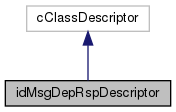
\includegraphics[width=204pt]{classid_msg_dep_rsp_descriptor__inherit__graph}
\end{center}
\end{figure}


Collaboration diagram for id\+Msg\+Dep\+Rsp\+Descriptor\+:\nopagebreak
\begin{figure}[H]
\begin{center}
\leavevmode
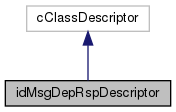
\includegraphics[width=204pt]{classid_msg_dep_rsp_descriptor__coll__graph}
\end{center}
\end{figure}
\subsection*{Public Member Functions}
\begin{DoxyCompactItemize}
\item 
\hyperlink{classid_msg_dep_rsp_descriptor_abedc396206c401b49a270bdc1bce5005}{id\+Msg\+Dep\+Rsp\+Descriptor} ()
\item 
virtual \hyperlink{classid_msg_dep_rsp_descriptor_acd48feffd371854f0d17b7201b672adf}{$\sim$id\+Msg\+Dep\+Rsp\+Descriptor} ()
\item 
virtual bool \hyperlink{classid_msg_dep_rsp_descriptor_a5e341b089472aeeb8a4854a7f4680794}{does\+Support} (omnetpp\+::c\+Object $\ast$obj) const override
\item 
virtual const char $\ast$$\ast$ \hyperlink{classid_msg_dep_rsp_descriptor_ac0d3a1bc5b63ebd0b88971dd6e2e2916}{get\+Property\+Names} () const override
\item 
virtual const char $\ast$ \hyperlink{classid_msg_dep_rsp_descriptor_a241bcfafb380d863d82e281b53c569d5}{get\+Property} (const char $\ast$propertyname) const override
\item 
virtual int \hyperlink{classid_msg_dep_rsp_descriptor_acac56df86dc592e4f75bfe669fbe7f4f}{get\+Field\+Count} () const override
\item 
virtual const char $\ast$ \hyperlink{classid_msg_dep_rsp_descriptor_adf1d3fbc7cac0f37939843ba3ebfcbe7}{get\+Field\+Name} (int field) const override
\item 
virtual int \hyperlink{classid_msg_dep_rsp_descriptor_a74b6bf9b08e70b9b91ee3e6765502af3}{find\+Field} (const char $\ast$field\+Name) const override
\item 
virtual unsigned int \hyperlink{classid_msg_dep_rsp_descriptor_a59b8fc18b2af7d74d95780a40e26b199}{get\+Field\+Type\+Flags} (int field) const override
\item 
virtual const char $\ast$ \hyperlink{classid_msg_dep_rsp_descriptor_ad3182b84a62c4607fe30506c392fa8af}{get\+Field\+Type\+String} (int field) const override
\item 
virtual const char $\ast$$\ast$ \hyperlink{classid_msg_dep_rsp_descriptor_a6a44113613dc717a215e94182ca73cb3}{get\+Field\+Property\+Names} (int field) const override
\item 
virtual const char $\ast$ \hyperlink{classid_msg_dep_rsp_descriptor_a522e2185bfa9e8833c180e4753c2f812}{get\+Field\+Property} (int field, const char $\ast$propertyname) const override
\item 
virtual int \hyperlink{classid_msg_dep_rsp_descriptor_a47159497c46236c093f395def9ea2601}{get\+Field\+Array\+Size} (void $\ast$object, int field) const override
\item 
virtual const char $\ast$ \hyperlink{classid_msg_dep_rsp_descriptor_af4fdd8255c6294f4c68d7a8ce3cec648}{get\+Field\+Dynamic\+Type\+String} (void $\ast$object, int field, int i) const override
\item 
virtual std\+::string \hyperlink{classid_msg_dep_rsp_descriptor_af28908b0998ae5028ce4439705a56bea}{get\+Field\+Value\+As\+String} (void $\ast$object, int field, int i) const override
\item 
virtual bool \hyperlink{classid_msg_dep_rsp_descriptor_a3b2b332f7e3426e7b6464a973de48013}{set\+Field\+Value\+As\+String} (void $\ast$object, int field, int i, const char $\ast$value) const override
\item 
virtual const char $\ast$ \hyperlink{classid_msg_dep_rsp_descriptor_a2c04a28f7d859199945889c5c1f1525f}{get\+Field\+Struct\+Name} (int field) const override
\item 
virtual void $\ast$ \hyperlink{classid_msg_dep_rsp_descriptor_a1c3f7a29a3bd609bcb9da8317720f673}{get\+Field\+Struct\+Value\+Pointer} (void $\ast$object, int field, int i) const override
\end{DoxyCompactItemize}
\subsection*{Private Attributes}
\begin{DoxyCompactItemize}
\item 
const char $\ast$$\ast$ \hyperlink{classid_msg_dep_rsp_descriptor_ab4be8a53831c1ebca93af83b99b3be40}{propertynames}
\end{DoxyCompactItemize}


\subsection{Constructor \& Destructor Documentation}
\mbox{\Hypertarget{classid_msg_dep_rsp_descriptor_abedc396206c401b49a270bdc1bce5005}\label{classid_msg_dep_rsp_descriptor_abedc396206c401b49a270bdc1bce5005}} 
\index{id\+Msg\+Dep\+Rsp\+Descriptor@{id\+Msg\+Dep\+Rsp\+Descriptor}!id\+Msg\+Dep\+Rsp\+Descriptor@{id\+Msg\+Dep\+Rsp\+Descriptor}}
\index{id\+Msg\+Dep\+Rsp\+Descriptor@{id\+Msg\+Dep\+Rsp\+Descriptor}!id\+Msg\+Dep\+Rsp\+Descriptor@{id\+Msg\+Dep\+Rsp\+Descriptor}}
\subsubsection{\texorpdfstring{id\+Msg\+Dep\+Rsp\+Descriptor()}{idMsgDepRspDescriptor()}}
{\footnotesize\ttfamily id\+Msg\+Dep\+Rsp\+Descriptor\+::id\+Msg\+Dep\+Rsp\+Descriptor (\begin{DoxyParamCaption}{ }\end{DoxyParamCaption})}

\mbox{\Hypertarget{classid_msg_dep_rsp_descriptor_acd48feffd371854f0d17b7201b672adf}\label{classid_msg_dep_rsp_descriptor_acd48feffd371854f0d17b7201b672adf}} 
\index{id\+Msg\+Dep\+Rsp\+Descriptor@{id\+Msg\+Dep\+Rsp\+Descriptor}!````~id\+Msg\+Dep\+Rsp\+Descriptor@{$\sim$id\+Msg\+Dep\+Rsp\+Descriptor}}
\index{````~id\+Msg\+Dep\+Rsp\+Descriptor@{$\sim$id\+Msg\+Dep\+Rsp\+Descriptor}!id\+Msg\+Dep\+Rsp\+Descriptor@{id\+Msg\+Dep\+Rsp\+Descriptor}}
\subsubsection{\texorpdfstring{$\sim$id\+Msg\+Dep\+Rsp\+Descriptor()}{~idMsgDepRspDescriptor()}}
{\footnotesize\ttfamily id\+Msg\+Dep\+Rsp\+Descriptor\+::$\sim$id\+Msg\+Dep\+Rsp\+Descriptor (\begin{DoxyParamCaption}{ }\end{DoxyParamCaption})\hspace{0.3cm}{\ttfamily [virtual]}}



\subsection{Member Function Documentation}
\mbox{\Hypertarget{classid_msg_dep_rsp_descriptor_a5e341b089472aeeb8a4854a7f4680794}\label{classid_msg_dep_rsp_descriptor_a5e341b089472aeeb8a4854a7f4680794}} 
\index{id\+Msg\+Dep\+Rsp\+Descriptor@{id\+Msg\+Dep\+Rsp\+Descriptor}!does\+Support@{does\+Support}}
\index{does\+Support@{does\+Support}!id\+Msg\+Dep\+Rsp\+Descriptor@{id\+Msg\+Dep\+Rsp\+Descriptor}}
\subsubsection{\texorpdfstring{does\+Support()}{doesSupport()}}
{\footnotesize\ttfamily bool id\+Msg\+Dep\+Rsp\+Descriptor\+::does\+Support (\begin{DoxyParamCaption}\item[{omnetpp\+::c\+Object $\ast$}]{obj }\end{DoxyParamCaption}) const\hspace{0.3cm}{\ttfamily [override]}, {\ttfamily [virtual]}}

\mbox{\Hypertarget{classid_msg_dep_rsp_descriptor_a74b6bf9b08e70b9b91ee3e6765502af3}\label{classid_msg_dep_rsp_descriptor_a74b6bf9b08e70b9b91ee3e6765502af3}} 
\index{id\+Msg\+Dep\+Rsp\+Descriptor@{id\+Msg\+Dep\+Rsp\+Descriptor}!find\+Field@{find\+Field}}
\index{find\+Field@{find\+Field}!id\+Msg\+Dep\+Rsp\+Descriptor@{id\+Msg\+Dep\+Rsp\+Descriptor}}
\subsubsection{\texorpdfstring{find\+Field()}{findField()}}
{\footnotesize\ttfamily int id\+Msg\+Dep\+Rsp\+Descriptor\+::find\+Field (\begin{DoxyParamCaption}\item[{const char $\ast$}]{field\+Name }\end{DoxyParamCaption}) const\hspace{0.3cm}{\ttfamily [override]}, {\ttfamily [virtual]}}

\mbox{\Hypertarget{classid_msg_dep_rsp_descriptor_a47159497c46236c093f395def9ea2601}\label{classid_msg_dep_rsp_descriptor_a47159497c46236c093f395def9ea2601}} 
\index{id\+Msg\+Dep\+Rsp\+Descriptor@{id\+Msg\+Dep\+Rsp\+Descriptor}!get\+Field\+Array\+Size@{get\+Field\+Array\+Size}}
\index{get\+Field\+Array\+Size@{get\+Field\+Array\+Size}!id\+Msg\+Dep\+Rsp\+Descriptor@{id\+Msg\+Dep\+Rsp\+Descriptor}}
\subsubsection{\texorpdfstring{get\+Field\+Array\+Size()}{getFieldArraySize()}}
{\footnotesize\ttfamily int id\+Msg\+Dep\+Rsp\+Descriptor\+::get\+Field\+Array\+Size (\begin{DoxyParamCaption}\item[{void $\ast$}]{object,  }\item[{int}]{field }\end{DoxyParamCaption}) const\hspace{0.3cm}{\ttfamily [override]}, {\ttfamily [virtual]}}

\mbox{\Hypertarget{classid_msg_dep_rsp_descriptor_acac56df86dc592e4f75bfe669fbe7f4f}\label{classid_msg_dep_rsp_descriptor_acac56df86dc592e4f75bfe669fbe7f4f}} 
\index{id\+Msg\+Dep\+Rsp\+Descriptor@{id\+Msg\+Dep\+Rsp\+Descriptor}!get\+Field\+Count@{get\+Field\+Count}}
\index{get\+Field\+Count@{get\+Field\+Count}!id\+Msg\+Dep\+Rsp\+Descriptor@{id\+Msg\+Dep\+Rsp\+Descriptor}}
\subsubsection{\texorpdfstring{get\+Field\+Count()}{getFieldCount()}}
{\footnotesize\ttfamily int id\+Msg\+Dep\+Rsp\+Descriptor\+::get\+Field\+Count (\begin{DoxyParamCaption}{ }\end{DoxyParamCaption}) const\hspace{0.3cm}{\ttfamily [override]}, {\ttfamily [virtual]}}

\mbox{\Hypertarget{classid_msg_dep_rsp_descriptor_af4fdd8255c6294f4c68d7a8ce3cec648}\label{classid_msg_dep_rsp_descriptor_af4fdd8255c6294f4c68d7a8ce3cec648}} 
\index{id\+Msg\+Dep\+Rsp\+Descriptor@{id\+Msg\+Dep\+Rsp\+Descriptor}!get\+Field\+Dynamic\+Type\+String@{get\+Field\+Dynamic\+Type\+String}}
\index{get\+Field\+Dynamic\+Type\+String@{get\+Field\+Dynamic\+Type\+String}!id\+Msg\+Dep\+Rsp\+Descriptor@{id\+Msg\+Dep\+Rsp\+Descriptor}}
\subsubsection{\texorpdfstring{get\+Field\+Dynamic\+Type\+String()}{getFieldDynamicTypeString()}}
{\footnotesize\ttfamily const char $\ast$ id\+Msg\+Dep\+Rsp\+Descriptor\+::get\+Field\+Dynamic\+Type\+String (\begin{DoxyParamCaption}\item[{void $\ast$}]{object,  }\item[{int}]{field,  }\item[{int}]{i }\end{DoxyParamCaption}) const\hspace{0.3cm}{\ttfamily [override]}, {\ttfamily [virtual]}}

\mbox{\Hypertarget{classid_msg_dep_rsp_descriptor_adf1d3fbc7cac0f37939843ba3ebfcbe7}\label{classid_msg_dep_rsp_descriptor_adf1d3fbc7cac0f37939843ba3ebfcbe7}} 
\index{id\+Msg\+Dep\+Rsp\+Descriptor@{id\+Msg\+Dep\+Rsp\+Descriptor}!get\+Field\+Name@{get\+Field\+Name}}
\index{get\+Field\+Name@{get\+Field\+Name}!id\+Msg\+Dep\+Rsp\+Descriptor@{id\+Msg\+Dep\+Rsp\+Descriptor}}
\subsubsection{\texorpdfstring{get\+Field\+Name()}{getFieldName()}}
{\footnotesize\ttfamily const char $\ast$ id\+Msg\+Dep\+Rsp\+Descriptor\+::get\+Field\+Name (\begin{DoxyParamCaption}\item[{int}]{field }\end{DoxyParamCaption}) const\hspace{0.3cm}{\ttfamily [override]}, {\ttfamily [virtual]}}

\mbox{\Hypertarget{classid_msg_dep_rsp_descriptor_a522e2185bfa9e8833c180e4753c2f812}\label{classid_msg_dep_rsp_descriptor_a522e2185bfa9e8833c180e4753c2f812}} 
\index{id\+Msg\+Dep\+Rsp\+Descriptor@{id\+Msg\+Dep\+Rsp\+Descriptor}!get\+Field\+Property@{get\+Field\+Property}}
\index{get\+Field\+Property@{get\+Field\+Property}!id\+Msg\+Dep\+Rsp\+Descriptor@{id\+Msg\+Dep\+Rsp\+Descriptor}}
\subsubsection{\texorpdfstring{get\+Field\+Property()}{getFieldProperty()}}
{\footnotesize\ttfamily const char $\ast$ id\+Msg\+Dep\+Rsp\+Descriptor\+::get\+Field\+Property (\begin{DoxyParamCaption}\item[{int}]{field,  }\item[{const char $\ast$}]{propertyname }\end{DoxyParamCaption}) const\hspace{0.3cm}{\ttfamily [override]}, {\ttfamily [virtual]}}

\mbox{\Hypertarget{classid_msg_dep_rsp_descriptor_a6a44113613dc717a215e94182ca73cb3}\label{classid_msg_dep_rsp_descriptor_a6a44113613dc717a215e94182ca73cb3}} 
\index{id\+Msg\+Dep\+Rsp\+Descriptor@{id\+Msg\+Dep\+Rsp\+Descriptor}!get\+Field\+Property\+Names@{get\+Field\+Property\+Names}}
\index{get\+Field\+Property\+Names@{get\+Field\+Property\+Names}!id\+Msg\+Dep\+Rsp\+Descriptor@{id\+Msg\+Dep\+Rsp\+Descriptor}}
\subsubsection{\texorpdfstring{get\+Field\+Property\+Names()}{getFieldPropertyNames()}}
{\footnotesize\ttfamily const char $\ast$$\ast$ id\+Msg\+Dep\+Rsp\+Descriptor\+::get\+Field\+Property\+Names (\begin{DoxyParamCaption}\item[{int}]{field }\end{DoxyParamCaption}) const\hspace{0.3cm}{\ttfamily [override]}, {\ttfamily [virtual]}}

\mbox{\Hypertarget{classid_msg_dep_rsp_descriptor_a2c04a28f7d859199945889c5c1f1525f}\label{classid_msg_dep_rsp_descriptor_a2c04a28f7d859199945889c5c1f1525f}} 
\index{id\+Msg\+Dep\+Rsp\+Descriptor@{id\+Msg\+Dep\+Rsp\+Descriptor}!get\+Field\+Struct\+Name@{get\+Field\+Struct\+Name}}
\index{get\+Field\+Struct\+Name@{get\+Field\+Struct\+Name}!id\+Msg\+Dep\+Rsp\+Descriptor@{id\+Msg\+Dep\+Rsp\+Descriptor}}
\subsubsection{\texorpdfstring{get\+Field\+Struct\+Name()}{getFieldStructName()}}
{\footnotesize\ttfamily const char $\ast$ id\+Msg\+Dep\+Rsp\+Descriptor\+::get\+Field\+Struct\+Name (\begin{DoxyParamCaption}\item[{int}]{field }\end{DoxyParamCaption}) const\hspace{0.3cm}{\ttfamily [override]}, {\ttfamily [virtual]}}

\mbox{\Hypertarget{classid_msg_dep_rsp_descriptor_a1c3f7a29a3bd609bcb9da8317720f673}\label{classid_msg_dep_rsp_descriptor_a1c3f7a29a3bd609bcb9da8317720f673}} 
\index{id\+Msg\+Dep\+Rsp\+Descriptor@{id\+Msg\+Dep\+Rsp\+Descriptor}!get\+Field\+Struct\+Value\+Pointer@{get\+Field\+Struct\+Value\+Pointer}}
\index{get\+Field\+Struct\+Value\+Pointer@{get\+Field\+Struct\+Value\+Pointer}!id\+Msg\+Dep\+Rsp\+Descriptor@{id\+Msg\+Dep\+Rsp\+Descriptor}}
\subsubsection{\texorpdfstring{get\+Field\+Struct\+Value\+Pointer()}{getFieldStructValuePointer()}}
{\footnotesize\ttfamily void $\ast$ id\+Msg\+Dep\+Rsp\+Descriptor\+::get\+Field\+Struct\+Value\+Pointer (\begin{DoxyParamCaption}\item[{void $\ast$}]{object,  }\item[{int}]{field,  }\item[{int}]{i }\end{DoxyParamCaption}) const\hspace{0.3cm}{\ttfamily [override]}, {\ttfamily [virtual]}}

\mbox{\Hypertarget{classid_msg_dep_rsp_descriptor_a59b8fc18b2af7d74d95780a40e26b199}\label{classid_msg_dep_rsp_descriptor_a59b8fc18b2af7d74d95780a40e26b199}} 
\index{id\+Msg\+Dep\+Rsp\+Descriptor@{id\+Msg\+Dep\+Rsp\+Descriptor}!get\+Field\+Type\+Flags@{get\+Field\+Type\+Flags}}
\index{get\+Field\+Type\+Flags@{get\+Field\+Type\+Flags}!id\+Msg\+Dep\+Rsp\+Descriptor@{id\+Msg\+Dep\+Rsp\+Descriptor}}
\subsubsection{\texorpdfstring{get\+Field\+Type\+Flags()}{getFieldTypeFlags()}}
{\footnotesize\ttfamily unsigned int id\+Msg\+Dep\+Rsp\+Descriptor\+::get\+Field\+Type\+Flags (\begin{DoxyParamCaption}\item[{int}]{field }\end{DoxyParamCaption}) const\hspace{0.3cm}{\ttfamily [override]}, {\ttfamily [virtual]}}

\mbox{\Hypertarget{classid_msg_dep_rsp_descriptor_ad3182b84a62c4607fe30506c392fa8af}\label{classid_msg_dep_rsp_descriptor_ad3182b84a62c4607fe30506c392fa8af}} 
\index{id\+Msg\+Dep\+Rsp\+Descriptor@{id\+Msg\+Dep\+Rsp\+Descriptor}!get\+Field\+Type\+String@{get\+Field\+Type\+String}}
\index{get\+Field\+Type\+String@{get\+Field\+Type\+String}!id\+Msg\+Dep\+Rsp\+Descriptor@{id\+Msg\+Dep\+Rsp\+Descriptor}}
\subsubsection{\texorpdfstring{get\+Field\+Type\+String()}{getFieldTypeString()}}
{\footnotesize\ttfamily const char $\ast$ id\+Msg\+Dep\+Rsp\+Descriptor\+::get\+Field\+Type\+String (\begin{DoxyParamCaption}\item[{int}]{field }\end{DoxyParamCaption}) const\hspace{0.3cm}{\ttfamily [override]}, {\ttfamily [virtual]}}

\mbox{\Hypertarget{classid_msg_dep_rsp_descriptor_af28908b0998ae5028ce4439705a56bea}\label{classid_msg_dep_rsp_descriptor_af28908b0998ae5028ce4439705a56bea}} 
\index{id\+Msg\+Dep\+Rsp\+Descriptor@{id\+Msg\+Dep\+Rsp\+Descriptor}!get\+Field\+Value\+As\+String@{get\+Field\+Value\+As\+String}}
\index{get\+Field\+Value\+As\+String@{get\+Field\+Value\+As\+String}!id\+Msg\+Dep\+Rsp\+Descriptor@{id\+Msg\+Dep\+Rsp\+Descriptor}}
\subsubsection{\texorpdfstring{get\+Field\+Value\+As\+String()}{getFieldValueAsString()}}
{\footnotesize\ttfamily std\+::string id\+Msg\+Dep\+Rsp\+Descriptor\+::get\+Field\+Value\+As\+String (\begin{DoxyParamCaption}\item[{void $\ast$}]{object,  }\item[{int}]{field,  }\item[{int}]{i }\end{DoxyParamCaption}) const\hspace{0.3cm}{\ttfamily [override]}, {\ttfamily [virtual]}}

\mbox{\Hypertarget{classid_msg_dep_rsp_descriptor_a241bcfafb380d863d82e281b53c569d5}\label{classid_msg_dep_rsp_descriptor_a241bcfafb380d863d82e281b53c569d5}} 
\index{id\+Msg\+Dep\+Rsp\+Descriptor@{id\+Msg\+Dep\+Rsp\+Descriptor}!get\+Property@{get\+Property}}
\index{get\+Property@{get\+Property}!id\+Msg\+Dep\+Rsp\+Descriptor@{id\+Msg\+Dep\+Rsp\+Descriptor}}
\subsubsection{\texorpdfstring{get\+Property()}{getProperty()}}
{\footnotesize\ttfamily const char $\ast$ id\+Msg\+Dep\+Rsp\+Descriptor\+::get\+Property (\begin{DoxyParamCaption}\item[{const char $\ast$}]{propertyname }\end{DoxyParamCaption}) const\hspace{0.3cm}{\ttfamily [override]}, {\ttfamily [virtual]}}

\mbox{\Hypertarget{classid_msg_dep_rsp_descriptor_ac0d3a1bc5b63ebd0b88971dd6e2e2916}\label{classid_msg_dep_rsp_descriptor_ac0d3a1bc5b63ebd0b88971dd6e2e2916}} 
\index{id\+Msg\+Dep\+Rsp\+Descriptor@{id\+Msg\+Dep\+Rsp\+Descriptor}!get\+Property\+Names@{get\+Property\+Names}}
\index{get\+Property\+Names@{get\+Property\+Names}!id\+Msg\+Dep\+Rsp\+Descriptor@{id\+Msg\+Dep\+Rsp\+Descriptor}}
\subsubsection{\texorpdfstring{get\+Property\+Names()}{getPropertyNames()}}
{\footnotesize\ttfamily const char $\ast$$\ast$ id\+Msg\+Dep\+Rsp\+Descriptor\+::get\+Property\+Names (\begin{DoxyParamCaption}{ }\end{DoxyParamCaption}) const\hspace{0.3cm}{\ttfamily [override]}, {\ttfamily [virtual]}}

\mbox{\Hypertarget{classid_msg_dep_rsp_descriptor_a3b2b332f7e3426e7b6464a973de48013}\label{classid_msg_dep_rsp_descriptor_a3b2b332f7e3426e7b6464a973de48013}} 
\index{id\+Msg\+Dep\+Rsp\+Descriptor@{id\+Msg\+Dep\+Rsp\+Descriptor}!set\+Field\+Value\+As\+String@{set\+Field\+Value\+As\+String}}
\index{set\+Field\+Value\+As\+String@{set\+Field\+Value\+As\+String}!id\+Msg\+Dep\+Rsp\+Descriptor@{id\+Msg\+Dep\+Rsp\+Descriptor}}
\subsubsection{\texorpdfstring{set\+Field\+Value\+As\+String()}{setFieldValueAsString()}}
{\footnotesize\ttfamily bool id\+Msg\+Dep\+Rsp\+Descriptor\+::set\+Field\+Value\+As\+String (\begin{DoxyParamCaption}\item[{void $\ast$}]{object,  }\item[{int}]{field,  }\item[{int}]{i,  }\item[{const char $\ast$}]{value }\end{DoxyParamCaption}) const\hspace{0.3cm}{\ttfamily [override]}, {\ttfamily [virtual]}}



\subsection{Member Data Documentation}
\mbox{\Hypertarget{classid_msg_dep_rsp_descriptor_ab4be8a53831c1ebca93af83b99b3be40}\label{classid_msg_dep_rsp_descriptor_ab4be8a53831c1ebca93af83b99b3be40}} 
\index{id\+Msg\+Dep\+Rsp\+Descriptor@{id\+Msg\+Dep\+Rsp\+Descriptor}!propertynames@{propertynames}}
\index{propertynames@{propertynames}!id\+Msg\+Dep\+Rsp\+Descriptor@{id\+Msg\+Dep\+Rsp\+Descriptor}}
\subsubsection{\texorpdfstring{propertynames}{propertynames}}
{\footnotesize\ttfamily const char$\ast$$\ast$ id\+Msg\+Dep\+Rsp\+Descriptor\+::propertynames\hspace{0.3cm}{\ttfamily [mutable]}, {\ttfamily [private]}}



The documentation for this class was generated from the following file\+:\begin{DoxyCompactItemize}
\item 
src/\+Messages/\hyperlink{dep_rsp__m_8cc}{dep\+Rsp\+\_\+m.\+cc}\end{DoxyCompactItemize}

\hypertarget{class_init}{}\section{Init Class Reference}
\label{class_init}\index{Init@{Init}}


Class generated from {\ttfamily Messages/\+Init.\+msg\+:19} by nedtool.  




{\ttfamily \#include $<$Init\+\_\+m.\+h$>$}



Inheritance diagram for Init\+:
\nopagebreak
\begin{figure}[H]
\begin{center}
\leavevmode
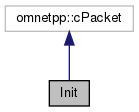
\includegraphics[width=176pt]{class_init__inherit__graph}
\end{center}
\end{figure}


Collaboration diagram for Init\+:
\nopagebreak
\begin{figure}[H]
\begin{center}
\leavevmode
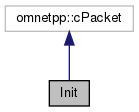
\includegraphics[width=176pt]{class_init__coll__graph}
\end{center}
\end{figure}
\subsection*{Public Member Functions}
\begin{DoxyCompactItemize}
\item 
\hyperlink{class_init_a763a386107f8ea21acfd24f243e0f73c}{Init} (const char $\ast$name=nullptr, short kind=0)
\item 
\hyperlink{class_init_a9d26400c5fabf20571808ad773524669}{Init} (const \hyperlink{class_init}{Init} \&other)
\item 
virtual \hyperlink{class_init_a67d5c94cb965fa3b774e969cfb4969d1}{$\sim$\+Init} ()
\item 
\hyperlink{class_init}{Init} \& \hyperlink{class_init_ab995dd231981ed97018c00b5fd8e9797}{operator=} (const \hyperlink{class_init}{Init} \&other)
\item 
virtual \hyperlink{class_init}{Init} $\ast$ \hyperlink{class_init_ad1e6c6b247eae6eaac5dd8e9dc9cdce0}{dup} () const override
\item 
virtual void \hyperlink{class_init_a73df5d54ec41b9980e98dbfc12875145}{parsim\+Pack} (omnetpp\+::c\+Comm\+Buffer $\ast$b) const override
\item 
virtual void \hyperlink{class_init_ab3728913400c516dbb31c8fed392d32d}{parsim\+Unpack} (omnetpp\+::c\+Comm\+Buffer $\ast$b) override
\item 
virtual unsigned int \hyperlink{class_init_a67fdac2389d7298a742e33a6551e8eb1}{get\+Node\+Id} () const
\item 
virtual void \hyperlink{class_init_a21b64722ff60f3ecf3b17939c0a1cb6d}{set\+Node\+Id} (unsigned int \hyperlink{class_init_abc9fcf6151621f0ac808cd29e14239c9}{node\+Id})
\end{DoxyCompactItemize}
\subsection*{Protected Member Functions}
\begin{DoxyCompactItemize}
\item 
bool \hyperlink{class_init_a474b7c9ffdf72a6b2b58558ce68bb03e}{operator==} (const \hyperlink{class_init}{Init} \&)
\end{DoxyCompactItemize}
\subsection*{Protected Attributes}
\begin{DoxyCompactItemize}
\item 
unsigned int \hyperlink{class_init_abc9fcf6151621f0ac808cd29e14239c9}{node\+Id}
\end{DoxyCompactItemize}
\subsection*{Private Member Functions}
\begin{DoxyCompactItemize}
\item 
void \hyperlink{class_init_a045745f591e312608e5ee3639f4459ba}{copy} (const \hyperlink{class_init}{Init} \&other)
\end{DoxyCompactItemize}


\subsection{Detailed Description}
Class generated from {\ttfamily Messages/\+Init.\+msg\+:19} by nedtool. 


\begin{DoxyPre}
//
// TODO generated message class
//
packet \hyperlink{class_init}{Init}
\{
    unsigned int nodeId;
\}
\end{DoxyPre}
 

\subsection{Constructor \& Destructor Documentation}
\mbox{\Hypertarget{class_init_a763a386107f8ea21acfd24f243e0f73c}\label{class_init_a763a386107f8ea21acfd24f243e0f73c}} 
\index{Init@{Init}!Init@{Init}}
\index{Init@{Init}!Init@{Init}}
\subsubsection{\texorpdfstring{Init()}{Init()}\hspace{0.1cm}{\footnotesize\ttfamily [1/2]}}
{\footnotesize\ttfamily Init\+::\+Init (\begin{DoxyParamCaption}\item[{const char $\ast$}]{name = {\ttfamily nullptr},  }\item[{short}]{kind = {\ttfamily 0} }\end{DoxyParamCaption})}

\mbox{\Hypertarget{class_init_a9d26400c5fabf20571808ad773524669}\label{class_init_a9d26400c5fabf20571808ad773524669}} 
\index{Init@{Init}!Init@{Init}}
\index{Init@{Init}!Init@{Init}}
\subsubsection{\texorpdfstring{Init()}{Init()}\hspace{0.1cm}{\footnotesize\ttfamily [2/2]}}
{\footnotesize\ttfamily Init\+::\+Init (\begin{DoxyParamCaption}\item[{const \hyperlink{class_init}{Init} \&}]{other }\end{DoxyParamCaption})}

\mbox{\Hypertarget{class_init_a67d5c94cb965fa3b774e969cfb4969d1}\label{class_init_a67d5c94cb965fa3b774e969cfb4969d1}} 
\index{Init@{Init}!````~Init@{$\sim$\+Init}}
\index{````~Init@{$\sim$\+Init}!Init@{Init}}
\subsubsection{\texorpdfstring{$\sim$\+Init()}{~Init()}}
{\footnotesize\ttfamily Init\+::$\sim$\+Init (\begin{DoxyParamCaption}{ }\end{DoxyParamCaption})\hspace{0.3cm}{\ttfamily [virtual]}}



\subsection{Member Function Documentation}
\mbox{\Hypertarget{class_init_a045745f591e312608e5ee3639f4459ba}\label{class_init_a045745f591e312608e5ee3639f4459ba}} 
\index{Init@{Init}!copy@{copy}}
\index{copy@{copy}!Init@{Init}}
\subsubsection{\texorpdfstring{copy()}{copy()}}
{\footnotesize\ttfamily void Init\+::copy (\begin{DoxyParamCaption}\item[{const \hyperlink{class_init}{Init} \&}]{other }\end{DoxyParamCaption})\hspace{0.3cm}{\ttfamily [private]}}

\mbox{\Hypertarget{class_init_ad1e6c6b247eae6eaac5dd8e9dc9cdce0}\label{class_init_ad1e6c6b247eae6eaac5dd8e9dc9cdce0}} 
\index{Init@{Init}!dup@{dup}}
\index{dup@{dup}!Init@{Init}}
\subsubsection{\texorpdfstring{dup()}{dup()}}
{\footnotesize\ttfamily virtual \hyperlink{class_init}{Init}$\ast$ Init\+::dup (\begin{DoxyParamCaption}{ }\end{DoxyParamCaption}) const\hspace{0.3cm}{\ttfamily [inline]}, {\ttfamily [override]}, {\ttfamily [virtual]}}

\mbox{\Hypertarget{class_init_a67fdac2389d7298a742e33a6551e8eb1}\label{class_init_a67fdac2389d7298a742e33a6551e8eb1}} 
\index{Init@{Init}!get\+Node\+Id@{get\+Node\+Id}}
\index{get\+Node\+Id@{get\+Node\+Id}!Init@{Init}}
\subsubsection{\texorpdfstring{get\+Node\+Id()}{getNodeId()}}
{\footnotesize\ttfamily unsigned int Init\+::get\+Node\+Id (\begin{DoxyParamCaption}{ }\end{DoxyParamCaption}) const\hspace{0.3cm}{\ttfamily [virtual]}}

\mbox{\Hypertarget{class_init_ab995dd231981ed97018c00b5fd8e9797}\label{class_init_ab995dd231981ed97018c00b5fd8e9797}} 
\index{Init@{Init}!operator=@{operator=}}
\index{operator=@{operator=}!Init@{Init}}
\subsubsection{\texorpdfstring{operator=()}{operator=()}}
{\footnotesize\ttfamily \hyperlink{class_init}{Init} \& Init\+::operator= (\begin{DoxyParamCaption}\item[{const \hyperlink{class_init}{Init} \&}]{other }\end{DoxyParamCaption})}

\mbox{\Hypertarget{class_init_a474b7c9ffdf72a6b2b58558ce68bb03e}\label{class_init_a474b7c9ffdf72a6b2b58558ce68bb03e}} 
\index{Init@{Init}!operator==@{operator==}}
\index{operator==@{operator==}!Init@{Init}}
\subsubsection{\texorpdfstring{operator==()}{operator==()}}
{\footnotesize\ttfamily bool Init\+::operator== (\begin{DoxyParamCaption}\item[{const \hyperlink{class_init}{Init} \&}]{ }\end{DoxyParamCaption})\hspace{0.3cm}{\ttfamily [protected]}}

\mbox{\Hypertarget{class_init_a73df5d54ec41b9980e98dbfc12875145}\label{class_init_a73df5d54ec41b9980e98dbfc12875145}} 
\index{Init@{Init}!parsim\+Pack@{parsim\+Pack}}
\index{parsim\+Pack@{parsim\+Pack}!Init@{Init}}
\subsubsection{\texorpdfstring{parsim\+Pack()}{parsimPack()}}
{\footnotesize\ttfamily void Init\+::parsim\+Pack (\begin{DoxyParamCaption}\item[{omnetpp\+::c\+Comm\+Buffer $\ast$}]{b }\end{DoxyParamCaption}) const\hspace{0.3cm}{\ttfamily [override]}, {\ttfamily [virtual]}}

\mbox{\Hypertarget{class_init_ab3728913400c516dbb31c8fed392d32d}\label{class_init_ab3728913400c516dbb31c8fed392d32d}} 
\index{Init@{Init}!parsim\+Unpack@{parsim\+Unpack}}
\index{parsim\+Unpack@{parsim\+Unpack}!Init@{Init}}
\subsubsection{\texorpdfstring{parsim\+Unpack()}{parsimUnpack()}}
{\footnotesize\ttfamily void Init\+::parsim\+Unpack (\begin{DoxyParamCaption}\item[{omnetpp\+::c\+Comm\+Buffer $\ast$}]{b }\end{DoxyParamCaption})\hspace{0.3cm}{\ttfamily [override]}, {\ttfamily [virtual]}}

\mbox{\Hypertarget{class_init_a21b64722ff60f3ecf3b17939c0a1cb6d}\label{class_init_a21b64722ff60f3ecf3b17939c0a1cb6d}} 
\index{Init@{Init}!set\+Node\+Id@{set\+Node\+Id}}
\index{set\+Node\+Id@{set\+Node\+Id}!Init@{Init}}
\subsubsection{\texorpdfstring{set\+Node\+Id()}{setNodeId()}}
{\footnotesize\ttfamily void Init\+::set\+Node\+Id (\begin{DoxyParamCaption}\item[{unsigned int}]{node\+Id }\end{DoxyParamCaption})\hspace{0.3cm}{\ttfamily [virtual]}}



\subsection{Member Data Documentation}
\mbox{\Hypertarget{class_init_abc9fcf6151621f0ac808cd29e14239c9}\label{class_init_abc9fcf6151621f0ac808cd29e14239c9}} 
\index{Init@{Init}!node\+Id@{node\+Id}}
\index{node\+Id@{node\+Id}!Init@{Init}}
\subsubsection{\texorpdfstring{node\+Id}{nodeId}}
{\footnotesize\ttfamily unsigned int Init\+::node\+Id\hspace{0.3cm}{\ttfamily [protected]}}



The documentation for this class was generated from the following files\+:\begin{DoxyCompactItemize}
\item 
/home/wilhelm/\+Documents/code\+Git\+Hub/\+Error\+Detectors/src/\+Messages/\hyperlink{_init__m_8h}{Init\+\_\+m.\+h}\item 
/home/wilhelm/\+Documents/code\+Git\+Hub/\+Error\+Detectors/src/\+Messages/\hyperlink{_init__m_8cc}{Init\+\_\+m.\+cc}\end{DoxyCompactItemize}

\hypertarget{class_init_descriptor}{}\section{Init\+Descriptor Class Reference}
\label{class_init_descriptor}\index{Init\+Descriptor@{Init\+Descriptor}}


Inheritance diagram for Init\+Descriptor\+:\nopagebreak
\begin{figure}[H]
\begin{center}
\leavevmode
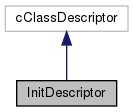
\includegraphics[width=172pt]{class_init_descriptor__inherit__graph}
\end{center}
\end{figure}


Collaboration diagram for Init\+Descriptor\+:\nopagebreak
\begin{figure}[H]
\begin{center}
\leavevmode
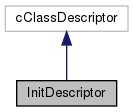
\includegraphics[width=172pt]{class_init_descriptor__coll__graph}
\end{center}
\end{figure}
\subsection*{Public Member Functions}
\begin{DoxyCompactItemize}
\item 
\hyperlink{class_init_descriptor_ab339ad8c646e3ebd54fca1d423669bcc}{Init\+Descriptor} ()
\item 
virtual \hyperlink{class_init_descriptor_a557046f2e1493c983f0dc57d67c48291}{$\sim$\+Init\+Descriptor} ()
\item 
virtual bool \hyperlink{class_init_descriptor_aa4691376d7b2f08fa800fff585125ea3}{does\+Support} (omnetpp\+::c\+Object $\ast$obj) const override
\item 
virtual const char $\ast$$\ast$ \hyperlink{class_init_descriptor_a50255fad26833319e82ea83650fa6eb9}{get\+Property\+Names} () const override
\item 
virtual const char $\ast$ \hyperlink{class_init_descriptor_a272a35c10d988eb431d03dd2d327512c}{get\+Property} (const char $\ast$propertyname) const override
\item 
virtual int \hyperlink{class_init_descriptor_ac70ed57d62820b4dd4bd68b55d4c8b10}{get\+Field\+Count} () const override
\item 
virtual const char $\ast$ \hyperlink{class_init_descriptor_a0c6fa440b30d1abd3d6e76f9845c6699}{get\+Field\+Name} (int field) const override
\item 
virtual int \hyperlink{class_init_descriptor_aa2e3648dd471c37754733337cbdccea0}{find\+Field} (const char $\ast$field\+Name) const override
\item 
virtual unsigned int \hyperlink{class_init_descriptor_ac608a1e528e9e41968ac118ff3c138e5}{get\+Field\+Type\+Flags} (int field) const override
\item 
virtual const char $\ast$ \hyperlink{class_init_descriptor_a5896b2cc03302e1b6f67168f0e9612e6}{get\+Field\+Type\+String} (int field) const override
\item 
virtual const char $\ast$$\ast$ \hyperlink{class_init_descriptor_a540feb97164ff9118592619a94887e35}{get\+Field\+Property\+Names} (int field) const override
\item 
virtual const char $\ast$ \hyperlink{class_init_descriptor_a9ec2bc98d856cb3166f66eab70eb6279}{get\+Field\+Property} (int field, const char $\ast$propertyname) const override
\item 
virtual int \hyperlink{class_init_descriptor_a7d04a2b854a3408ae32479cfb5eeb253}{get\+Field\+Array\+Size} (void $\ast$object, int field) const override
\item 
virtual const char $\ast$ \hyperlink{class_init_descriptor_a93d85a84c15e095b2eb7b39b2b392837}{get\+Field\+Dynamic\+Type\+String} (void $\ast$object, int field, int i) const override
\item 
virtual std\+::string \hyperlink{class_init_descriptor_a94c8aa0ca2f12dff66033c5320e944bb}{get\+Field\+Value\+As\+String} (void $\ast$object, int field, int i) const override
\item 
virtual bool \hyperlink{class_init_descriptor_af57482db7fb146d3da8b790900a3f96e}{set\+Field\+Value\+As\+String} (void $\ast$object, int field, int i, const char $\ast$value) const override
\item 
virtual const char $\ast$ \hyperlink{class_init_descriptor_a13c89c76ac3273c48418e94eab1c88b0}{get\+Field\+Struct\+Name} (int field) const override
\item 
virtual void $\ast$ \hyperlink{class_init_descriptor_a40bdb3ccca5709afd21ab2a2bf12b5e0}{get\+Field\+Struct\+Value\+Pointer} (void $\ast$object, int field, int i) const override
\end{DoxyCompactItemize}
\subsection*{Private Attributes}
\begin{DoxyCompactItemize}
\item 
const char $\ast$$\ast$ \hyperlink{class_init_descriptor_a070498d1650ac65184f35f6449f7cd5d}{propertynames}
\end{DoxyCompactItemize}


\subsection{Constructor \& Destructor Documentation}
\mbox{\Hypertarget{class_init_descriptor_ab339ad8c646e3ebd54fca1d423669bcc}\label{class_init_descriptor_ab339ad8c646e3ebd54fca1d423669bcc}} 
\index{Init\+Descriptor@{Init\+Descriptor}!Init\+Descriptor@{Init\+Descriptor}}
\index{Init\+Descriptor@{Init\+Descriptor}!Init\+Descriptor@{Init\+Descriptor}}
\subsubsection{\texorpdfstring{Init\+Descriptor()}{InitDescriptor()}}
{\footnotesize\ttfamily Init\+Descriptor\+::\+Init\+Descriptor (\begin{DoxyParamCaption}{ }\end{DoxyParamCaption})}

\mbox{\Hypertarget{class_init_descriptor_a557046f2e1493c983f0dc57d67c48291}\label{class_init_descriptor_a557046f2e1493c983f0dc57d67c48291}} 
\index{Init\+Descriptor@{Init\+Descriptor}!````~Init\+Descriptor@{$\sim$\+Init\+Descriptor}}
\index{````~Init\+Descriptor@{$\sim$\+Init\+Descriptor}!Init\+Descriptor@{Init\+Descriptor}}
\subsubsection{\texorpdfstring{$\sim$\+Init\+Descriptor()}{~InitDescriptor()}}
{\footnotesize\ttfamily Init\+Descriptor\+::$\sim$\+Init\+Descriptor (\begin{DoxyParamCaption}{ }\end{DoxyParamCaption})\hspace{0.3cm}{\ttfamily [virtual]}}



\subsection{Member Function Documentation}
\mbox{\Hypertarget{class_init_descriptor_aa4691376d7b2f08fa800fff585125ea3}\label{class_init_descriptor_aa4691376d7b2f08fa800fff585125ea3}} 
\index{Init\+Descriptor@{Init\+Descriptor}!does\+Support@{does\+Support}}
\index{does\+Support@{does\+Support}!Init\+Descriptor@{Init\+Descriptor}}
\subsubsection{\texorpdfstring{does\+Support()}{doesSupport()}}
{\footnotesize\ttfamily bool Init\+Descriptor\+::does\+Support (\begin{DoxyParamCaption}\item[{omnetpp\+::c\+Object $\ast$}]{obj }\end{DoxyParamCaption}) const\hspace{0.3cm}{\ttfamily [override]}, {\ttfamily [virtual]}}

\mbox{\Hypertarget{class_init_descriptor_aa2e3648dd471c37754733337cbdccea0}\label{class_init_descriptor_aa2e3648dd471c37754733337cbdccea0}} 
\index{Init\+Descriptor@{Init\+Descriptor}!find\+Field@{find\+Field}}
\index{find\+Field@{find\+Field}!Init\+Descriptor@{Init\+Descriptor}}
\subsubsection{\texorpdfstring{find\+Field()}{findField()}}
{\footnotesize\ttfamily int Init\+Descriptor\+::find\+Field (\begin{DoxyParamCaption}\item[{const char $\ast$}]{field\+Name }\end{DoxyParamCaption}) const\hspace{0.3cm}{\ttfamily [override]}, {\ttfamily [virtual]}}

\mbox{\Hypertarget{class_init_descriptor_a7d04a2b854a3408ae32479cfb5eeb253}\label{class_init_descriptor_a7d04a2b854a3408ae32479cfb5eeb253}} 
\index{Init\+Descriptor@{Init\+Descriptor}!get\+Field\+Array\+Size@{get\+Field\+Array\+Size}}
\index{get\+Field\+Array\+Size@{get\+Field\+Array\+Size}!Init\+Descriptor@{Init\+Descriptor}}
\subsubsection{\texorpdfstring{get\+Field\+Array\+Size()}{getFieldArraySize()}}
{\footnotesize\ttfamily int Init\+Descriptor\+::get\+Field\+Array\+Size (\begin{DoxyParamCaption}\item[{void $\ast$}]{object,  }\item[{int}]{field }\end{DoxyParamCaption}) const\hspace{0.3cm}{\ttfamily [override]}, {\ttfamily [virtual]}}

\mbox{\Hypertarget{class_init_descriptor_ac70ed57d62820b4dd4bd68b55d4c8b10}\label{class_init_descriptor_ac70ed57d62820b4dd4bd68b55d4c8b10}} 
\index{Init\+Descriptor@{Init\+Descriptor}!get\+Field\+Count@{get\+Field\+Count}}
\index{get\+Field\+Count@{get\+Field\+Count}!Init\+Descriptor@{Init\+Descriptor}}
\subsubsection{\texorpdfstring{get\+Field\+Count()}{getFieldCount()}}
{\footnotesize\ttfamily int Init\+Descriptor\+::get\+Field\+Count (\begin{DoxyParamCaption}{ }\end{DoxyParamCaption}) const\hspace{0.3cm}{\ttfamily [override]}, {\ttfamily [virtual]}}

\mbox{\Hypertarget{class_init_descriptor_a93d85a84c15e095b2eb7b39b2b392837}\label{class_init_descriptor_a93d85a84c15e095b2eb7b39b2b392837}} 
\index{Init\+Descriptor@{Init\+Descriptor}!get\+Field\+Dynamic\+Type\+String@{get\+Field\+Dynamic\+Type\+String}}
\index{get\+Field\+Dynamic\+Type\+String@{get\+Field\+Dynamic\+Type\+String}!Init\+Descriptor@{Init\+Descriptor}}
\subsubsection{\texorpdfstring{get\+Field\+Dynamic\+Type\+String()}{getFieldDynamicTypeString()}}
{\footnotesize\ttfamily const char $\ast$ Init\+Descriptor\+::get\+Field\+Dynamic\+Type\+String (\begin{DoxyParamCaption}\item[{void $\ast$}]{object,  }\item[{int}]{field,  }\item[{int}]{i }\end{DoxyParamCaption}) const\hspace{0.3cm}{\ttfamily [override]}, {\ttfamily [virtual]}}

\mbox{\Hypertarget{class_init_descriptor_a0c6fa440b30d1abd3d6e76f9845c6699}\label{class_init_descriptor_a0c6fa440b30d1abd3d6e76f9845c6699}} 
\index{Init\+Descriptor@{Init\+Descriptor}!get\+Field\+Name@{get\+Field\+Name}}
\index{get\+Field\+Name@{get\+Field\+Name}!Init\+Descriptor@{Init\+Descriptor}}
\subsubsection{\texorpdfstring{get\+Field\+Name()}{getFieldName()}}
{\footnotesize\ttfamily const char $\ast$ Init\+Descriptor\+::get\+Field\+Name (\begin{DoxyParamCaption}\item[{int}]{field }\end{DoxyParamCaption}) const\hspace{0.3cm}{\ttfamily [override]}, {\ttfamily [virtual]}}

\mbox{\Hypertarget{class_init_descriptor_a9ec2bc98d856cb3166f66eab70eb6279}\label{class_init_descriptor_a9ec2bc98d856cb3166f66eab70eb6279}} 
\index{Init\+Descriptor@{Init\+Descriptor}!get\+Field\+Property@{get\+Field\+Property}}
\index{get\+Field\+Property@{get\+Field\+Property}!Init\+Descriptor@{Init\+Descriptor}}
\subsubsection{\texorpdfstring{get\+Field\+Property()}{getFieldProperty()}}
{\footnotesize\ttfamily const char $\ast$ Init\+Descriptor\+::get\+Field\+Property (\begin{DoxyParamCaption}\item[{int}]{field,  }\item[{const char $\ast$}]{propertyname }\end{DoxyParamCaption}) const\hspace{0.3cm}{\ttfamily [override]}, {\ttfamily [virtual]}}

\mbox{\Hypertarget{class_init_descriptor_a540feb97164ff9118592619a94887e35}\label{class_init_descriptor_a540feb97164ff9118592619a94887e35}} 
\index{Init\+Descriptor@{Init\+Descriptor}!get\+Field\+Property\+Names@{get\+Field\+Property\+Names}}
\index{get\+Field\+Property\+Names@{get\+Field\+Property\+Names}!Init\+Descriptor@{Init\+Descriptor}}
\subsubsection{\texorpdfstring{get\+Field\+Property\+Names()}{getFieldPropertyNames()}}
{\footnotesize\ttfamily const char $\ast$$\ast$ Init\+Descriptor\+::get\+Field\+Property\+Names (\begin{DoxyParamCaption}\item[{int}]{field }\end{DoxyParamCaption}) const\hspace{0.3cm}{\ttfamily [override]}, {\ttfamily [virtual]}}

\mbox{\Hypertarget{class_init_descriptor_a13c89c76ac3273c48418e94eab1c88b0}\label{class_init_descriptor_a13c89c76ac3273c48418e94eab1c88b0}} 
\index{Init\+Descriptor@{Init\+Descriptor}!get\+Field\+Struct\+Name@{get\+Field\+Struct\+Name}}
\index{get\+Field\+Struct\+Name@{get\+Field\+Struct\+Name}!Init\+Descriptor@{Init\+Descriptor}}
\subsubsection{\texorpdfstring{get\+Field\+Struct\+Name()}{getFieldStructName()}}
{\footnotesize\ttfamily const char $\ast$ Init\+Descriptor\+::get\+Field\+Struct\+Name (\begin{DoxyParamCaption}\item[{int}]{field }\end{DoxyParamCaption}) const\hspace{0.3cm}{\ttfamily [override]}, {\ttfamily [virtual]}}

\mbox{\Hypertarget{class_init_descriptor_a40bdb3ccca5709afd21ab2a2bf12b5e0}\label{class_init_descriptor_a40bdb3ccca5709afd21ab2a2bf12b5e0}} 
\index{Init\+Descriptor@{Init\+Descriptor}!get\+Field\+Struct\+Value\+Pointer@{get\+Field\+Struct\+Value\+Pointer}}
\index{get\+Field\+Struct\+Value\+Pointer@{get\+Field\+Struct\+Value\+Pointer}!Init\+Descriptor@{Init\+Descriptor}}
\subsubsection{\texorpdfstring{get\+Field\+Struct\+Value\+Pointer()}{getFieldStructValuePointer()}}
{\footnotesize\ttfamily void $\ast$ Init\+Descriptor\+::get\+Field\+Struct\+Value\+Pointer (\begin{DoxyParamCaption}\item[{void $\ast$}]{object,  }\item[{int}]{field,  }\item[{int}]{i }\end{DoxyParamCaption}) const\hspace{0.3cm}{\ttfamily [override]}, {\ttfamily [virtual]}}

\mbox{\Hypertarget{class_init_descriptor_ac608a1e528e9e41968ac118ff3c138e5}\label{class_init_descriptor_ac608a1e528e9e41968ac118ff3c138e5}} 
\index{Init\+Descriptor@{Init\+Descriptor}!get\+Field\+Type\+Flags@{get\+Field\+Type\+Flags}}
\index{get\+Field\+Type\+Flags@{get\+Field\+Type\+Flags}!Init\+Descriptor@{Init\+Descriptor}}
\subsubsection{\texorpdfstring{get\+Field\+Type\+Flags()}{getFieldTypeFlags()}}
{\footnotesize\ttfamily unsigned int Init\+Descriptor\+::get\+Field\+Type\+Flags (\begin{DoxyParamCaption}\item[{int}]{field }\end{DoxyParamCaption}) const\hspace{0.3cm}{\ttfamily [override]}, {\ttfamily [virtual]}}

\mbox{\Hypertarget{class_init_descriptor_a5896b2cc03302e1b6f67168f0e9612e6}\label{class_init_descriptor_a5896b2cc03302e1b6f67168f0e9612e6}} 
\index{Init\+Descriptor@{Init\+Descriptor}!get\+Field\+Type\+String@{get\+Field\+Type\+String}}
\index{get\+Field\+Type\+String@{get\+Field\+Type\+String}!Init\+Descriptor@{Init\+Descriptor}}
\subsubsection{\texorpdfstring{get\+Field\+Type\+String()}{getFieldTypeString()}}
{\footnotesize\ttfamily const char $\ast$ Init\+Descriptor\+::get\+Field\+Type\+String (\begin{DoxyParamCaption}\item[{int}]{field }\end{DoxyParamCaption}) const\hspace{0.3cm}{\ttfamily [override]}, {\ttfamily [virtual]}}

\mbox{\Hypertarget{class_init_descriptor_a94c8aa0ca2f12dff66033c5320e944bb}\label{class_init_descriptor_a94c8aa0ca2f12dff66033c5320e944bb}} 
\index{Init\+Descriptor@{Init\+Descriptor}!get\+Field\+Value\+As\+String@{get\+Field\+Value\+As\+String}}
\index{get\+Field\+Value\+As\+String@{get\+Field\+Value\+As\+String}!Init\+Descriptor@{Init\+Descriptor}}
\subsubsection{\texorpdfstring{get\+Field\+Value\+As\+String()}{getFieldValueAsString()}}
{\footnotesize\ttfamily std\+::string Init\+Descriptor\+::get\+Field\+Value\+As\+String (\begin{DoxyParamCaption}\item[{void $\ast$}]{object,  }\item[{int}]{field,  }\item[{int}]{i }\end{DoxyParamCaption}) const\hspace{0.3cm}{\ttfamily [override]}, {\ttfamily [virtual]}}

\mbox{\Hypertarget{class_init_descriptor_a272a35c10d988eb431d03dd2d327512c}\label{class_init_descriptor_a272a35c10d988eb431d03dd2d327512c}} 
\index{Init\+Descriptor@{Init\+Descriptor}!get\+Property@{get\+Property}}
\index{get\+Property@{get\+Property}!Init\+Descriptor@{Init\+Descriptor}}
\subsubsection{\texorpdfstring{get\+Property()}{getProperty()}}
{\footnotesize\ttfamily const char $\ast$ Init\+Descriptor\+::get\+Property (\begin{DoxyParamCaption}\item[{const char $\ast$}]{propertyname }\end{DoxyParamCaption}) const\hspace{0.3cm}{\ttfamily [override]}, {\ttfamily [virtual]}}

\mbox{\Hypertarget{class_init_descriptor_a50255fad26833319e82ea83650fa6eb9}\label{class_init_descriptor_a50255fad26833319e82ea83650fa6eb9}} 
\index{Init\+Descriptor@{Init\+Descriptor}!get\+Property\+Names@{get\+Property\+Names}}
\index{get\+Property\+Names@{get\+Property\+Names}!Init\+Descriptor@{Init\+Descriptor}}
\subsubsection{\texorpdfstring{get\+Property\+Names()}{getPropertyNames()}}
{\footnotesize\ttfamily const char $\ast$$\ast$ Init\+Descriptor\+::get\+Property\+Names (\begin{DoxyParamCaption}{ }\end{DoxyParamCaption}) const\hspace{0.3cm}{\ttfamily [override]}, {\ttfamily [virtual]}}

\mbox{\Hypertarget{class_init_descriptor_af57482db7fb146d3da8b790900a3f96e}\label{class_init_descriptor_af57482db7fb146d3da8b790900a3f96e}} 
\index{Init\+Descriptor@{Init\+Descriptor}!set\+Field\+Value\+As\+String@{set\+Field\+Value\+As\+String}}
\index{set\+Field\+Value\+As\+String@{set\+Field\+Value\+As\+String}!Init\+Descriptor@{Init\+Descriptor}}
\subsubsection{\texorpdfstring{set\+Field\+Value\+As\+String()}{setFieldValueAsString()}}
{\footnotesize\ttfamily bool Init\+Descriptor\+::set\+Field\+Value\+As\+String (\begin{DoxyParamCaption}\item[{void $\ast$}]{object,  }\item[{int}]{field,  }\item[{int}]{i,  }\item[{const char $\ast$}]{value }\end{DoxyParamCaption}) const\hspace{0.3cm}{\ttfamily [override]}, {\ttfamily [virtual]}}



\subsection{Member Data Documentation}
\mbox{\Hypertarget{class_init_descriptor_a070498d1650ac65184f35f6449f7cd5d}\label{class_init_descriptor_a070498d1650ac65184f35f6449f7cd5d}} 
\index{Init\+Descriptor@{Init\+Descriptor}!propertynames@{propertynames}}
\index{propertynames@{propertynames}!Init\+Descriptor@{Init\+Descriptor}}
\subsubsection{\texorpdfstring{propertynames}{propertynames}}
{\footnotesize\ttfamily const char$\ast$$\ast$ Init\+Descriptor\+::propertynames\hspace{0.3cm}{\ttfamily [mutable]}, {\ttfamily [private]}}



The documentation for this class was generated from the following file\+:\begin{DoxyCompactItemize}
\item 
src/\+Messages/\hyperlink{_init__m_8cc}{Init\+\_\+m.\+cc}\end{DoxyCompactItemize}

\hypertarget{class_mostefaoui_error_detector}{}\section{Mostefaoui\+Error\+Detector Class Reference}
\label{class_mostefaoui_error_detector}\index{Mostefaoui\+Error\+Detector@{Mostefaoui\+Error\+Detector}}


Error detector proposed by Mostéfaoui and Weiss.  




{\ttfamily \#include $<$Mostefaoui\+Error\+Detector.\+h$>$}



Inheritance diagram for Mostefaoui\+Error\+Detector\+:\nopagebreak
\begin{figure}[H]
\begin{center}
\leavevmode
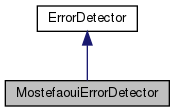
\includegraphics[width=203pt]{class_mostefaoui_error_detector__inherit__graph}
\end{center}
\end{figure}


Collaboration diagram for Mostefaoui\+Error\+Detector\+:\nopagebreak
\begin{figure}[H]
\begin{center}
\leavevmode
\includegraphics[width=203pt]{class_mostefaoui_error_detector__coll__graph}
\end{center}
\end{figure}
\subsection*{Public Member Functions}
\begin{DoxyCompactItemize}
\item 
\hyperlink{class_mostefaoui_error_detector_a2a76ea0d2e986ce379c5686f48f887dc}{Mostefaoui\+Error\+Detector} ()
\item 
virtual \hyperlink{class_mostefaoui_error_detector_a8658848d90c291c1364962c0759ca806}{$\sim$\+Mostefaoui\+Error\+Detector} ()
\item 
virtual bool \hyperlink{class_mostefaoui_error_detector_a293f6cf144526bc8694fc4f1fc0daeb5}{test} (\hyperlink{structures_8h_a7e7bdc1d2fff8a9436f2f352b2711ed6}{message\+Info} message, const vector$<$ unsigned int $>$ \&incremented\+Clock\+Entries, const \hyperlink{class_probabilistic_clock}{Probabilistic\+Clock} \&process\+Clock, const \hyperlink{class_total_dependencies}{Total\+Dependencies} \&process\+Dependencies, \hyperlink{class_controller}{Controller} $\ast$control, \hyperlink{class_simulation_parameters}{Simulation\+Parameters} $\ast$params, const vector$<$ \hyperlink{structures_8h_a7e7bdc1d2fff8a9436f2f352b2711ed6}{message\+Info} $>$ \&delivered)
\begin{DoxyCompactList}\small\item\em Error detector test to determine if the message to deliver can be delivered in causal order. \end{DoxyCompactList}\item 
virtual \hyperlink{class_app_msg}{App\+Msg} $\ast$ \hyperlink{class_mostefaoui_error_detector_adcd530d7349df19adb614ca414225214}{prepare\+Message} (\hyperlink{class_app_msg}{App\+Msg} $\ast$m, const vector$<$ \hyperlink{structures_8h_a7e7bdc1d2fff8a9436f2f352b2711ed6}{message\+Info} $>$ \&delivered, const \hyperlink{class_probabilistic_clock}{Probabilistic\+Clock} \&clock, const \hyperlink{class_total_dependencies}{Total\+Dependencies} \&process\+Dependencies)
\begin{DoxyCompactList}\small\item\em Appends to the message to broadcast the information the destination error detector requires. \end{DoxyCompactList}\end{DoxyCompactItemize}


\subsection{Detailed Description}
Error detector proposed by Mostéfaoui and Weiss. 



\subsection{Constructor \& Destructor Documentation}
\mbox{\Hypertarget{class_mostefaoui_error_detector_a2a76ea0d2e986ce379c5686f48f887dc}\label{class_mostefaoui_error_detector_a2a76ea0d2e986ce379c5686f48f887dc}} 
\index{Mostefaoui\+Error\+Detector@{Mostefaoui\+Error\+Detector}!Mostefaoui\+Error\+Detector@{Mostefaoui\+Error\+Detector}}
\index{Mostefaoui\+Error\+Detector@{Mostefaoui\+Error\+Detector}!Mostefaoui\+Error\+Detector@{Mostefaoui\+Error\+Detector}}
\subsubsection{\texorpdfstring{Mostefaoui\+Error\+Detector()}{MostefaouiErrorDetector()}}
{\footnotesize\ttfamily Mostefaoui\+Error\+Detector\+::\+Mostefaoui\+Error\+Detector (\begin{DoxyParamCaption}{ }\end{DoxyParamCaption})}

\mbox{\Hypertarget{class_mostefaoui_error_detector_a8658848d90c291c1364962c0759ca806}\label{class_mostefaoui_error_detector_a8658848d90c291c1364962c0759ca806}} 
\index{Mostefaoui\+Error\+Detector@{Mostefaoui\+Error\+Detector}!````~Mostefaoui\+Error\+Detector@{$\sim$\+Mostefaoui\+Error\+Detector}}
\index{````~Mostefaoui\+Error\+Detector@{$\sim$\+Mostefaoui\+Error\+Detector}!Mostefaoui\+Error\+Detector@{Mostefaoui\+Error\+Detector}}
\subsubsection{\texorpdfstring{$\sim$\+Mostefaoui\+Error\+Detector()}{~MostefaouiErrorDetector()}}
{\footnotesize\ttfamily Mostefaoui\+Error\+Detector\+::$\sim$\+Mostefaoui\+Error\+Detector (\begin{DoxyParamCaption}{ }\end{DoxyParamCaption})\hspace{0.3cm}{\ttfamily [virtual]}}



\subsection{Member Function Documentation}
\mbox{\Hypertarget{class_mostefaoui_error_detector_adcd530d7349df19adb614ca414225214}\label{class_mostefaoui_error_detector_adcd530d7349df19adb614ca414225214}} 
\index{Mostefaoui\+Error\+Detector@{Mostefaoui\+Error\+Detector}!prepare\+Message@{prepare\+Message}}
\index{prepare\+Message@{prepare\+Message}!Mostefaoui\+Error\+Detector@{Mostefaoui\+Error\+Detector}}
\subsubsection{\texorpdfstring{prepare\+Message()}{prepareMessage()}}
{\footnotesize\ttfamily \hyperlink{class_app_msg}{App\+Msg} $\ast$ Mostefaoui\+Error\+Detector\+::prepare\+Message (\begin{DoxyParamCaption}\item[{\hyperlink{class_app_msg}{App\+Msg} $\ast$}]{m,  }\item[{const vector$<$ \hyperlink{structures_8h_a7e7bdc1d2fff8a9436f2f352b2711ed6}{message\+Info} $>$ \&}]{delivered,  }\item[{const \hyperlink{class_probabilistic_clock}{Probabilistic\+Clock} \&}]{clock,  }\item[{const \hyperlink{class_total_dependencies}{Total\+Dependencies} \&}]{process\+Dependencies }\end{DoxyParamCaption})\hspace{0.3cm}{\ttfamily [virtual]}}



Appends to the message to broadcast the information the destination error detector requires. 



Implements \hyperlink{class_error_detector_a8cac1f6ac6803da4379df7891789c490}{Error\+Detector}.

\mbox{\Hypertarget{class_mostefaoui_error_detector_a293f6cf144526bc8694fc4f1fc0daeb5}\label{class_mostefaoui_error_detector_a293f6cf144526bc8694fc4f1fc0daeb5}} 
\index{Mostefaoui\+Error\+Detector@{Mostefaoui\+Error\+Detector}!test@{test}}
\index{test@{test}!Mostefaoui\+Error\+Detector@{Mostefaoui\+Error\+Detector}}
\subsubsection{\texorpdfstring{test()}{test()}}
{\footnotesize\ttfamily bool Mostefaoui\+Error\+Detector\+::test (\begin{DoxyParamCaption}\item[{\hyperlink{structures_8h_a7e7bdc1d2fff8a9436f2f352b2711ed6}{message\+Info}}]{message,  }\item[{const vector$<$ unsigned int $>$ \&}]{incremented\+Clock\+Entries,  }\item[{const \hyperlink{class_probabilistic_clock}{Probabilistic\+Clock} \&}]{process\+Clock,  }\item[{const \hyperlink{class_total_dependencies}{Total\+Dependencies} \&}]{process\+Dependencies,  }\item[{\hyperlink{class_controller}{Controller} $\ast$}]{control,  }\item[{\hyperlink{class_simulation_parameters}{Simulation\+Parameters} $\ast$}]{params,  }\item[{const vector$<$ \hyperlink{structures_8h_a7e7bdc1d2fff8a9436f2f352b2711ed6}{message\+Info} $>$ \&}]{delivered }\end{DoxyParamCaption})\hspace{0.3cm}{\ttfamily [virtual]}}



Error detector test to determine if the message to deliver can be delivered in causal order. 



Implements \hyperlink{class_error_detector_afc717d04768dd207196c08e24163115c}{Error\+Detector}.



The documentation for this class was generated from the following files\+:\begin{DoxyCompactItemize}
\item 
src/\+Detectors/\hyperlink{_mostefaoui_error_detector_8h}{Mostefaoui\+Error\+Detector.\+h}\item 
src/\+Detectors/\hyperlink{_mostefaoui_error_detector_8cc}{Mostefaoui\+Error\+Detector.\+cc}\end{DoxyCompactItemize}

\hypertarget{class_node_base}{}\section{Node\+Base Class Reference}
\label{class_node_base}\index{Node\+Base@{Node\+Base}}


Base class of Nodes.  




{\ttfamily \#include $<$Node\+Base.\+h$>$}



Inheritance diagram for Node\+Base\+:\nopagebreak
\begin{figure}[H]
\begin{center}
\leavevmode
\includegraphics[width=326pt]{class_node_base__inherit__graph}
\end{center}
\end{figure}


Collaboration diagram for Node\+Base\+:
\nopagebreak
\begin{figure}[H]
\begin{center}
\leavevmode
\includegraphics[width=350pt]{class_node_base__coll__graph}
\end{center}
\end{figure}
\subsection*{Protected Member Functions}
\begin{DoxyCompactItemize}
\item 
\hyperlink{class_node_base_ab6ea4e77947d5b9b8da66d37dc432e7f}{Node\+Base} ()
\item 
virtual \hyperlink{class_node_base_a2fd7f7080282b6af95ba0b09fd30679d}{$\sim$\+Node\+Base} ()
\item 
virtual void \hyperlink{class_node_base_af7910c39553111295b66c88742d1198a}{initialize} () override
\begin{DoxyCompactList}\small\item\em Initializes the node by scheduling it\textquotesingle{}s broadcast\+Timer, initializing its connection with the communication dispatcher and looking up the \hyperlink{class_simulation_parameters}{Simulation\+Parameters} and \hyperlink{class_controller}{Controller} modules. \end{DoxyCompactList}\item 
void \hyperlink{class_node_base_a2077b2a599f55050603268dbf8fff6a7}{initialize\+Communications} ()
\begin{DoxyCompactList}\small\item\em Initializes the connection with the communication\+Dispatcher by sending an \hyperlink{class_init}{Init} message containing the node\textquotesingle{}s id, such that the communication\+Dispatcher can associate the gates to the right nodes. \end{DoxyCompactList}\item 
virtual void \hyperlink{class_node_base_add2450264be5dd616f9f9ac94e83b988}{handle\+Message} (c\+Message $\ast$\hyperlink{_controller_8h_afa0f3b802fbc219228f7bb97996fa558}{msg}) override
\begin{DoxyCompactList}\small\item\em Called upon reception of a message to proecss it, whether it be a selfmsg (broadcast\+Timer) or a message received from another process. \end{DoxyCompactList}\item 
void \hyperlink{class_node_base_a65273f043d18d6f021199fba050700b5}{handle\+Broadcast\+Timer} (c\+Message $\ast$\hyperlink{_controller_8h_afa0f3b802fbc219228f7bb97996fa558}{msg})
\begin{DoxyCompactList}\small\item\em Called to handle the broadcast\+Timer. \end{DoxyCompactList}\item 
virtual \hyperlink{class_app_msg}{App\+Msg} $\ast$ \hyperlink{class_node_base_a66c1dee9d15119bc3e68da71067ff6cd}{prepare\+Broadcast} ()
\begin{DoxyCompactList}\small\item\em Prepares the broadcast of an application message by creating it and notifying the controller of the broadcast. \end{DoxyCompactList}\item 
virtual \hyperlink{class_app_msg}{App\+Msg} $\ast$ \hyperlink{class_node_base_ac8b9e21b1cc32fd86aaa6c956b93a7c3}{create\+App\+Msg} ()
\begin{DoxyCompactList}\small\item\em Creates an application message and initializes it. \end{DoxyCompactList}\item 
virtual void \hyperlink{class_node_base_ae70b168f2bc7407c249594b1c614301c}{process\+Message} (c\+Message $\ast$\hyperlink{_controller_8h_afa0f3b802fbc219228f7bb97996fa558}{msg})=0
\begin{DoxyCompactList}\small\item\em Called at reception of messages from other nodes in order to process them. \end{DoxyCompactList}\item 
virtual bool \hyperlink{class_node_base_a49052382add1123da26db6bfb687d254}{deliver\+Msg} (const \hyperlink{structures_8h_a7e7bdc1d2fff8a9436f2f352b2711ed6}{message\+Info} \&message)
\begin{DoxyCompactList}\small\item\em Delivers a message and verifies its delivery in causal order. \end{DoxyCompactList}\end{DoxyCompactItemize}
\subsection*{Protected Attributes}
\begin{DoxyCompactItemize}
\item 
const unsigned int \hyperlink{class_node_base_a2924723bf530b8304c5e028504aafd84}{id} = \hyperlink{class_node_base_a3d577a517665ac5bcf9ed9495945fe31}{id\+Counter}++
\begin{DoxyCompactList}\small\item\em Unique identificator of the process. \end{DoxyCompactList}\item 
unsigned int \hyperlink{class_node_base_a4fe5b1b7aeb49d15ec7986133346aeb7}{seq} = 0
\begin{DoxyCompactList}\small\item\em Sequence number counter the process uses to give a unique identificator to messages. \end{DoxyCompactList}\item 
c\+Message $\ast$ \hyperlink{class_node_base_a8b7bd31bf2bef92de75a2b565c42fd8a}{broadcast\+Timer} = new c\+Message()
\begin{DoxyCompactList}\small\item\em Timer to scheduel the broadcast of application messages. \end{DoxyCompactList}\item 
simtime\+\_\+t \hyperlink{class_node_base_a199676fc8bd0203c7241f58779c5921c}{base\+Time\+Broadcast}
\begin{DoxyCompactList}\small\item\em Time of first message broadcast. \end{DoxyCompactList}\item 
std\+::default\+\_\+random\+\_\+engine \hyperlink{class_node_base_a2c488fd8adf4d208593a6e6eba4d6220}{generator\+Send\+Distribution}
\begin{DoxyCompactList}\small\item\em Used to have a random variation in the broadcast time of application messages. \end{DoxyCompactList}\item 
c\+Gate $\ast$ \hyperlink{class_node_base_a2e86bd53e181f8b488130032da547f8e}{out\+Gate}
\begin{DoxyCompactList}\small\item\em Gate used to communicate with other nodes. \end{DoxyCompactList}\item 
\hyperlink{class_simulation_parameters}{Simulation\+Parameters} $\ast$ \hyperlink{class_node_base_aa6fb61208e4f5b7a841cd46fac297058}{params}
\begin{DoxyCompactList}\small\item\em Reference to the simulation parameters to avoid looking them up in each function. \end{DoxyCompactList}\item 
\hyperlink{_node_base_8h_a6d83bdf09c8e309d31f9330091b0d10d}{stats\+Node} \hyperlink{class_node_base_a12b20bca634637499bf55020c398424e}{stats}
\begin{DoxyCompactList}\small\item\em \hyperlink{class_stats}{Stats} relevant to all types of nodes. \end{DoxyCompactList}\item 
\hyperlink{class_controller}{Controller} $\ast$ \hyperlink{class_node_base_a89bfb79efc25d9508eb15a4184558c41}{control}
\begin{DoxyCompactList}\small\item\em Reference to the controller module to avoid looking it up every time. \end{DoxyCompactList}\end{DoxyCompactItemize}
\subsection*{Static Protected Attributes}
\begin{DoxyCompactItemize}
\item 
static std\+::normal\+\_\+distribution$<$ double $>$ \hyperlink{class_node_base_ab8e4cc30083c58d14b22d928a78cb8ac}{send\+Distribution} = std\+::normal\+\_\+distribution$<$double$>$(0.,10000.)
\begin{DoxyCompactList}\small\item\em Used to have a random variation in the broadcast time of application messages. \end{DoxyCompactList}\end{DoxyCompactItemize}
\subsection*{Static Private Attributes}
\begin{DoxyCompactItemize}
\item 
static unsigned int \hyperlink{class_node_base_a3d577a517665ac5bcf9ed9495945fe31}{id\+Counter} = 0
\begin{DoxyCompactList}\small\item\em Counter used to give a unique identificator to every node. \end{DoxyCompactList}\end{DoxyCompactItemize}
\subsection*{Friends}
\begin{DoxyCompactItemize}
\item 
class \hyperlink{class_node_base_a129f65b6976377739eb6231b6962985e}{Stats}
\end{DoxyCompactItemize}


\subsection{Detailed Description}
Base class of Nodes. 

\subsection{Constructor \& Destructor Documentation}
\mbox{\Hypertarget{class_node_base_ab6ea4e77947d5b9b8da66d37dc432e7f}\label{class_node_base_ab6ea4e77947d5b9b8da66d37dc432e7f}} 
\index{Node\+Base@{Node\+Base}!Node\+Base@{Node\+Base}}
\index{Node\+Base@{Node\+Base}!Node\+Base@{Node\+Base}}
\subsubsection{\texorpdfstring{Node\+Base()}{NodeBase()}}
{\footnotesize\ttfamily Node\+Base\+::\+Node\+Base (\begin{DoxyParamCaption}{ }\end{DoxyParamCaption})\hspace{0.3cm}{\ttfamily [protected]}}

\mbox{\Hypertarget{class_node_base_a2fd7f7080282b6af95ba0b09fd30679d}\label{class_node_base_a2fd7f7080282b6af95ba0b09fd30679d}} 
\index{Node\+Base@{Node\+Base}!````~Node\+Base@{$\sim$\+Node\+Base}}
\index{````~Node\+Base@{$\sim$\+Node\+Base}!Node\+Base@{Node\+Base}}
\subsubsection{\texorpdfstring{$\sim$\+Node\+Base()}{~NodeBase()}}
{\footnotesize\ttfamily Node\+Base\+::$\sim$\+Node\+Base (\begin{DoxyParamCaption}{ }\end{DoxyParamCaption})\hspace{0.3cm}{\ttfamily [protected]}, {\ttfamily [virtual]}}



\subsection{Member Function Documentation}
\mbox{\Hypertarget{class_node_base_ac8b9e21b1cc32fd86aaa6c956b93a7c3}\label{class_node_base_ac8b9e21b1cc32fd86aaa6c956b93a7c3}} 
\index{Node\+Base@{Node\+Base}!create\+App\+Msg@{create\+App\+Msg}}
\index{create\+App\+Msg@{create\+App\+Msg}!Node\+Base@{Node\+Base}}
\subsubsection{\texorpdfstring{create\+App\+Msg()}{createAppMsg()}}
{\footnotesize\ttfamily \hyperlink{class_app_msg}{App\+Msg} $\ast$ Node\+Base\+::create\+App\+Msg (\begin{DoxyParamCaption}{ }\end{DoxyParamCaption})\hspace{0.3cm}{\ttfamily [protected]}, {\ttfamily [virtual]}}



Creates an application message and initializes it. 

\begin{DoxyReturn}{Returns}
The application message. 
\end{DoxyReturn}


Reimplemented in \hyperlink{class_node_with_control_a7772568c2836f5f204952ebe659e0049}{Node\+With\+Control}, and \hyperlink{class_node_detector_a7100349647350ad5e3aeb1ed4669c723}{Node\+Detector}.

\mbox{\Hypertarget{class_node_base_a49052382add1123da26db6bfb687d254}\label{class_node_base_a49052382add1123da26db6bfb687d254}} 
\index{Node\+Base@{Node\+Base}!deliver\+Msg@{deliver\+Msg}}
\index{deliver\+Msg@{deliver\+Msg}!Node\+Base@{Node\+Base}}
\subsubsection{\texorpdfstring{deliver\+Msg()}{deliverMsg()}}
{\footnotesize\ttfamily bool Node\+Base\+::deliver\+Msg (\begin{DoxyParamCaption}\item[{const \hyperlink{structures_8h_a7e7bdc1d2fff8a9436f2f352b2711ed6}{message\+Info} \&}]{message }\end{DoxyParamCaption})\hspace{0.3cm}{\ttfamily [protected]}, {\ttfamily [virtual]}}



Delivers a message and verifies its delivery in causal order. 


\begin{DoxyParams}{Parameters}
{\em message} & The information about the message to deliver. \\
\hline
\end{DoxyParams}
\begin{DoxyReturn}{Returns}
true if the message has been delivered in causal order and false otherwise. 
\end{DoxyReturn}


Reimplemented in \hyperlink{class_node_with_control_aada7451be61be592b27188b6249afef2}{Node\+With\+Control}.

\mbox{\Hypertarget{class_node_base_a65273f043d18d6f021199fba050700b5}\label{class_node_base_a65273f043d18d6f021199fba050700b5}} 
\index{Node\+Base@{Node\+Base}!handle\+Broadcast\+Timer@{handle\+Broadcast\+Timer}}
\index{handle\+Broadcast\+Timer@{handle\+Broadcast\+Timer}!Node\+Base@{Node\+Base}}
\subsubsection{\texorpdfstring{handle\+Broadcast\+Timer()}{handleBroadcastTimer()}}
{\footnotesize\ttfamily void Node\+Base\+::handle\+Broadcast\+Timer (\begin{DoxyParamCaption}\item[{c\+Message $\ast$}]{msg }\end{DoxyParamCaption})\hspace{0.3cm}{\ttfamily [protected]}}



Called to handle the broadcast\+Timer. 

Determines the first broadcast time at the beginning of the simulation, and broadcasts messages and schedules next broadcasts otherwise. 
\begin{DoxyParams}{Parameters}
{\em msg} & Timer used to schedule the next broadcast of application messages. \\
\hline
\end{DoxyParams}
\mbox{\Hypertarget{class_node_base_add2450264be5dd616f9f9ac94e83b988}\label{class_node_base_add2450264be5dd616f9f9ac94e83b988}} 
\index{Node\+Base@{Node\+Base}!handle\+Message@{handle\+Message}}
\index{handle\+Message@{handle\+Message}!Node\+Base@{Node\+Base}}
\subsubsection{\texorpdfstring{handle\+Message()}{handleMessage()}}
{\footnotesize\ttfamily void Node\+Base\+::handle\+Message (\begin{DoxyParamCaption}\item[{c\+Message $\ast$}]{msg }\end{DoxyParamCaption})\hspace{0.3cm}{\ttfamily [override]}, {\ttfamily [protected]}, {\ttfamily [virtual]}}



Called upon reception of a message to proecss it, whether it be a selfmsg (broadcast\+Timer) or a message received from another process. 


\begin{DoxyParams}{Parameters}
{\em msg} & The message the node received. \\
\hline
\end{DoxyParams}


Reimplemented in \hyperlink{class_node_with_recovery_a901c89606b84898e13fe8a66228acd9f}{Node\+With\+Recovery}.

\mbox{\Hypertarget{class_node_base_af7910c39553111295b66c88742d1198a}\label{class_node_base_af7910c39553111295b66c88742d1198a}} 
\index{Node\+Base@{Node\+Base}!initialize@{initialize}}
\index{initialize@{initialize}!Node\+Base@{Node\+Base}}
\subsubsection{\texorpdfstring{initialize()}{initialize()}}
{\footnotesize\ttfamily void Node\+Base\+::initialize (\begin{DoxyParamCaption}{ }\end{DoxyParamCaption})\hspace{0.3cm}{\ttfamily [override]}, {\ttfamily [protected]}, {\ttfamily [virtual]}}



Initializes the node by scheduling it\textquotesingle{}s broadcast\+Timer, initializing its connection with the communication dispatcher and looking up the \hyperlink{class_simulation_parameters}{Simulation\+Parameters} and \hyperlink{class_controller}{Controller} modules. 



Reimplemented in \hyperlink{class_node_with_control_a08c8e80fd67b52c51c642d7c66fe729c}{Node\+With\+Control}, and \hyperlink{class_node_detector_aefa188ab0657837b1b57f24674d3ef22}{Node\+Detector}.

\mbox{\Hypertarget{class_node_base_a2077b2a599f55050603268dbf8fff6a7}\label{class_node_base_a2077b2a599f55050603268dbf8fff6a7}} 
\index{Node\+Base@{Node\+Base}!initialize\+Communications@{initialize\+Communications}}
\index{initialize\+Communications@{initialize\+Communications}!Node\+Base@{Node\+Base}}
\subsubsection{\texorpdfstring{initialize\+Communications()}{initializeCommunications()}}
{\footnotesize\ttfamily void Node\+Base\+::initialize\+Communications (\begin{DoxyParamCaption}{ }\end{DoxyParamCaption})\hspace{0.3cm}{\ttfamily [protected]}}



Initializes the connection with the communication\+Dispatcher by sending an \hyperlink{class_init}{Init} message containing the node\textquotesingle{}s id, such that the communication\+Dispatcher can associate the gates to the right nodes. 

\mbox{\Hypertarget{class_node_base_a66c1dee9d15119bc3e68da71067ff6cd}\label{class_node_base_a66c1dee9d15119bc3e68da71067ff6cd}} 
\index{Node\+Base@{Node\+Base}!prepare\+Broadcast@{prepare\+Broadcast}}
\index{prepare\+Broadcast@{prepare\+Broadcast}!Node\+Base@{Node\+Base}}
\subsubsection{\texorpdfstring{prepare\+Broadcast()}{prepareBroadcast()}}
{\footnotesize\ttfamily \hyperlink{class_app_msg}{App\+Msg} $\ast$ Node\+Base\+::prepare\+Broadcast (\begin{DoxyParamCaption}{ }\end{DoxyParamCaption})\hspace{0.3cm}{\ttfamily [protected]}, {\ttfamily [virtual]}}



Prepares the broadcast of an application message by creating it and notifying the controller of the broadcast. 

\begin{DoxyReturn}{Returns}
The application message to broadcast. 
\end{DoxyReturn}


Reimplemented in \hyperlink{class_node_with_recovery_a33d8e8775fd69cb647b38a54b36e1ebe}{Node\+With\+Recovery}, \hyperlink{class_node_with_control_ab871014cf3f42d834f8d34ad5498174c}{Node\+With\+Control}, and \hyperlink{class_node_detector_af75cf37cc01fc51bc228a7a83c10cb97}{Node\+Detector}.

\mbox{\Hypertarget{class_node_base_ae70b168f2bc7407c249594b1c614301c}\label{class_node_base_ae70b168f2bc7407c249594b1c614301c}} 
\index{Node\+Base@{Node\+Base}!process\+Message@{process\+Message}}
\index{process\+Message@{process\+Message}!Node\+Base@{Node\+Base}}
\subsubsection{\texorpdfstring{process\+Message()}{processMessage()}}
{\footnotesize\ttfamily virtual void Node\+Base\+::process\+Message (\begin{DoxyParamCaption}\item[{c\+Message $\ast$}]{msg }\end{DoxyParamCaption})\hspace{0.3cm}{\ttfamily [protected]}, {\ttfamily [pure virtual]}}



Called at reception of messages from other nodes in order to process them. 



Implemented in \hyperlink{class_node_with_recovery_a216c29d76ddb0e94cd5701ff208c7f5b}{Node\+With\+Recovery}, \hyperlink{class_node_with_control_af532082fab76c38d8c50ca90e991f4c3}{Node\+With\+Control}, \hyperlink{class_node_detector_ab69432c6d3327a684845ec231826727e}{Node\+Detector}, \hyperlink{class_node_no_control_aa83bc408fe3dab03f124ea5489946836}{Node\+No\+Control}, \hyperlink{class_node_p_c_aa5fedc4136104a06e2f1131f1ba16b0e}{Node\+PC}, and \hyperlink{class_node_without_recovery_a0b44132b4ebc650399711766cb050399}{Node\+Without\+Recovery}.



\subsection{Friends And Related Function Documentation}
\mbox{\Hypertarget{class_node_base_a129f65b6976377739eb6231b6962985e}\label{class_node_base_a129f65b6976377739eb6231b6962985e}} 
\index{Node\+Base@{Node\+Base}!Stats@{Stats}}
\index{Stats@{Stats}!Node\+Base@{Node\+Base}}
\subsubsection{\texorpdfstring{Stats}{Stats}}
{\footnotesize\ttfamily friend class \hyperlink{class_stats}{Stats}\hspace{0.3cm}{\ttfamily [friend]}}



\subsection{Member Data Documentation}
\mbox{\Hypertarget{class_node_base_a199676fc8bd0203c7241f58779c5921c}\label{class_node_base_a199676fc8bd0203c7241f58779c5921c}} 
\index{Node\+Base@{Node\+Base}!base\+Time\+Broadcast@{base\+Time\+Broadcast}}
\index{base\+Time\+Broadcast@{base\+Time\+Broadcast}!Node\+Base@{Node\+Base}}
\subsubsection{\texorpdfstring{base\+Time\+Broadcast}{baseTimeBroadcast}}
{\footnotesize\ttfamily simtime\+\_\+t Node\+Base\+::base\+Time\+Broadcast\hspace{0.3cm}{\ttfamily [protected]}}



Time of first message broadcast. 

\mbox{\Hypertarget{class_node_base_a8b7bd31bf2bef92de75a2b565c42fd8a}\label{class_node_base_a8b7bd31bf2bef92de75a2b565c42fd8a}} 
\index{Node\+Base@{Node\+Base}!broadcast\+Timer@{broadcast\+Timer}}
\index{broadcast\+Timer@{broadcast\+Timer}!Node\+Base@{Node\+Base}}
\subsubsection{\texorpdfstring{broadcast\+Timer}{broadcastTimer}}
{\footnotesize\ttfamily c\+Message$\ast$ Node\+Base\+::broadcast\+Timer = new c\+Message()\hspace{0.3cm}{\ttfamily [protected]}}



Timer to scheduel the broadcast of application messages. 

\mbox{\Hypertarget{class_node_base_a89bfb79efc25d9508eb15a4184558c41}\label{class_node_base_a89bfb79efc25d9508eb15a4184558c41}} 
\index{Node\+Base@{Node\+Base}!control@{control}}
\index{control@{control}!Node\+Base@{Node\+Base}}
\subsubsection{\texorpdfstring{control}{control}}
{\footnotesize\ttfamily \hyperlink{class_controller}{Controller}$\ast$ Node\+Base\+::control\hspace{0.3cm}{\ttfamily [protected]}}



Reference to the controller module to avoid looking it up every time. 

\mbox{\Hypertarget{class_node_base_a2c488fd8adf4d208593a6e6eba4d6220}\label{class_node_base_a2c488fd8adf4d208593a6e6eba4d6220}} 
\index{Node\+Base@{Node\+Base}!generator\+Send\+Distribution@{generator\+Send\+Distribution}}
\index{generator\+Send\+Distribution@{generator\+Send\+Distribution}!Node\+Base@{Node\+Base}}
\subsubsection{\texorpdfstring{generator\+Send\+Distribution}{generatorSendDistribution}}
{\footnotesize\ttfamily std\+::default\+\_\+random\+\_\+engine Node\+Base\+::generator\+Send\+Distribution\hspace{0.3cm}{\ttfamily [protected]}}



Used to have a random variation in the broadcast time of application messages. 

Each node broadcast a message at base\+Time\+Broadcast + send\+Delay + variable\+Delay, with variable\+Delay generated with that random engine. \mbox{\Hypertarget{class_node_base_a2924723bf530b8304c5e028504aafd84}\label{class_node_base_a2924723bf530b8304c5e028504aafd84}} 
\index{Node\+Base@{Node\+Base}!id@{id}}
\index{id@{id}!Node\+Base@{Node\+Base}}
\subsubsection{\texorpdfstring{id}{id}}
{\footnotesize\ttfamily const unsigned int Node\+Base\+::id = \hyperlink{class_node_base_a3d577a517665ac5bcf9ed9495945fe31}{id\+Counter}++\hspace{0.3cm}{\ttfamily [protected]}}



Unique identificator of the process. 

\mbox{\Hypertarget{class_node_base_a3d577a517665ac5bcf9ed9495945fe31}\label{class_node_base_a3d577a517665ac5bcf9ed9495945fe31}} 
\index{Node\+Base@{Node\+Base}!id\+Counter@{id\+Counter}}
\index{id\+Counter@{id\+Counter}!Node\+Base@{Node\+Base}}
\subsubsection{\texorpdfstring{id\+Counter}{idCounter}}
{\footnotesize\ttfamily unsigned int Node\+Base\+::id\+Counter = 0\hspace{0.3cm}{\ttfamily [static]}, {\ttfamily [private]}}



Counter used to give a unique identificator to every node. 

\mbox{\Hypertarget{class_node_base_a2e86bd53e181f8b488130032da547f8e}\label{class_node_base_a2e86bd53e181f8b488130032da547f8e}} 
\index{Node\+Base@{Node\+Base}!out\+Gate@{out\+Gate}}
\index{out\+Gate@{out\+Gate}!Node\+Base@{Node\+Base}}
\subsubsection{\texorpdfstring{out\+Gate}{outGate}}
{\footnotesize\ttfamily c\+Gate$\ast$ Node\+Base\+::out\+Gate\hspace{0.3cm}{\ttfamily [protected]}}



Gate used to communicate with other nodes. 

\mbox{\Hypertarget{class_node_base_aa6fb61208e4f5b7a841cd46fac297058}\label{class_node_base_aa6fb61208e4f5b7a841cd46fac297058}} 
\index{Node\+Base@{Node\+Base}!params@{params}}
\index{params@{params}!Node\+Base@{Node\+Base}}
\subsubsection{\texorpdfstring{params}{params}}
{\footnotesize\ttfamily \hyperlink{class_simulation_parameters}{Simulation\+Parameters}$\ast$ Node\+Base\+::params\hspace{0.3cm}{\ttfamily [protected]}}



Reference to the simulation parameters to avoid looking them up in each function. 

\mbox{\Hypertarget{class_node_base_ab8e4cc30083c58d14b22d928a78cb8ac}\label{class_node_base_ab8e4cc30083c58d14b22d928a78cb8ac}} 
\index{Node\+Base@{Node\+Base}!send\+Distribution@{send\+Distribution}}
\index{send\+Distribution@{send\+Distribution}!Node\+Base@{Node\+Base}}
\subsubsection{\texorpdfstring{send\+Distribution}{sendDistribution}}
{\footnotesize\ttfamily std\+::normal\+\_\+distribution$<$ double $>$ Node\+Base\+::send\+Distribution = std\+::normal\+\_\+distribution$<$double$>$(0.,10000.)\hspace{0.3cm}{\ttfamily [static]}, {\ttfamily [protected]}}



Used to have a random variation in the broadcast time of application messages. 

\mbox{\Hypertarget{class_node_base_a4fe5b1b7aeb49d15ec7986133346aeb7}\label{class_node_base_a4fe5b1b7aeb49d15ec7986133346aeb7}} 
\index{Node\+Base@{Node\+Base}!seq@{seq}}
\index{seq@{seq}!Node\+Base@{Node\+Base}}
\subsubsection{\texorpdfstring{seq}{seq}}
{\footnotesize\ttfamily unsigned int Node\+Base\+::seq = 0\hspace{0.3cm}{\ttfamily [protected]}}



Sequence number counter the process uses to give a unique identificator to messages. 

\mbox{\Hypertarget{class_node_base_a12b20bca634637499bf55020c398424e}\label{class_node_base_a12b20bca634637499bf55020c398424e}} 
\index{Node\+Base@{Node\+Base}!stats@{stats}}
\index{stats@{stats}!Node\+Base@{Node\+Base}}
\subsubsection{\texorpdfstring{stats}{stats}}
{\footnotesize\ttfamily \hyperlink{_node_base_8h_a6d83bdf09c8e309d31f9330091b0d10d}{stats\+Node} Node\+Base\+::stats\hspace{0.3cm}{\ttfamily [protected]}}



\hyperlink{class_stats}{Stats} relevant to all types of nodes. 



The documentation for this class was generated from the following files\+:\begin{DoxyCompactItemize}
\item 
src/\+Nodes/\hyperlink{_node_base_8h}{Node\+Base.\+h}\item 
src/\+Nodes/\hyperlink{_node_base_8cc}{Node\+Base.\+cc}\end{DoxyCompactItemize}

\hypertarget{class_node_detector}{}\section{Node\+Detector Class Reference}
\label{class_node_detector}\index{Node\+Detector@{Node\+Detector}}


Base class to implement nodes using error detectors.  




{\ttfamily \#include $<$Node\+Detector.\+h$>$}



Inheritance diagram for Node\+Detector\+:
\nopagebreak
\begin{figure}[H]
\begin{center}
\leavevmode
\includegraphics[width=326pt]{class_node_detector__inherit__graph}
\end{center}
\end{figure}


Collaboration diagram for Node\+Detector\+:
\nopagebreak
\begin{figure}[H]
\begin{center}
\leavevmode
\includegraphics[width=350pt]{class_node_detector__coll__graph}
\end{center}
\end{figure}
\subsection*{Protected Member Functions}
\begin{DoxyCompactItemize}
\item 
\hyperlink{class_node_detector_a256160d034631f4fa14a83787f504aae}{Node\+Detector} ()
\item 
virtual \hyperlink{class_node_detector_a3f8e6eedfce05ea8953ff1a41413ccfa}{$\sim$\+Node\+Detector} ()
\item 
virtual void \hyperlink{class_node_detector_aefa188ab0657837b1b57f24674d3ef22}{initialize} () override
\begin{DoxyCompactList}\small\item\em Initializes the node by instantiating the error detector following the simulation parameters. \end{DoxyCompactList}\item 
\hyperlink{class_app_msg}{App\+Msg} $\ast$ \hyperlink{class_node_detector_a7100349647350ad5e3aeb1ed4669c723}{create\+App\+Msg} ()
\begin{DoxyCompactList}\small\item\em Instantiates an application message. \end{DoxyCompactList}\item 
\hyperlink{class_app_msg}{App\+Msg} $\ast$ \hyperlink{class_node_detector_af75cf37cc01fc51bc228a7a83c10cb97}{prepare\+Broadcast} ()
\begin{DoxyCompactList}\small\item\em Prepares the message\textquotesingle{}s broadcast. \end{DoxyCompactList}\item 
virtual void \hyperlink{class_node_detector_ab69432c6d3327a684845ec231826727e}{process\+Message} (c\+Message $\ast$\hyperlink{_controller_8h_afa0f3b802fbc219228f7bb97996fa558}{msg})=0
\begin{DoxyCompactList}\small\item\em Processes messages the process received (self messages and messages received from other nodes). \end{DoxyCompactList}\item 
virtual bool \hyperlink{class_node_detector_a51e7dccd54e94bbe937752ca39dfdba4}{test\+Deliver\+Message} (const \hyperlink{structures_8h_a7e7bdc1d2fff8a9436f2f352b2711ed6}{message\+Info} \&message)=0
\begin{DoxyCompactList}\small\item\em Tries to deliver a message. \end{DoxyCompactList}\item 
virtual void \hyperlink{class_node_detector_a17ecf9939fce7471f4513b66185743cc}{iterative\+Delivery} ()=0
\begin{DoxyCompactList}\small\item\em Tries to deliver pending messages. \end{DoxyCompactList}\end{DoxyCompactItemize}
\subsection*{Protected Attributes}
\begin{DoxyCompactItemize}
\item 
\hyperlink{class_error_detector}{Error\+Detector} $\ast$ \hyperlink{class_node_detector_a711fd643dc29b74e6dfe87e1aeb1b227}{detector}
\begin{DoxyCompactList}\small\item\em Error detector used to analyze messages before delivering them. \end{DoxyCompactList}\end{DoxyCompactItemize}
\subsection*{Friends}
\begin{DoxyCompactItemize}
\item 
class \hyperlink{class_node_detector_a129f65b6976377739eb6231b6962985e}{Stats}
\end{DoxyCompactItemize}
\subsection*{Additional Inherited Members}


\subsection{Detailed Description}
Base class to implement nodes using error detectors. 

\subsection{Constructor \& Destructor Documentation}
\mbox{\Hypertarget{class_node_detector_a256160d034631f4fa14a83787f504aae}\label{class_node_detector_a256160d034631f4fa14a83787f504aae}} 
\index{Node\+Detector@{Node\+Detector}!Node\+Detector@{Node\+Detector}}
\index{Node\+Detector@{Node\+Detector}!Node\+Detector@{Node\+Detector}}
\subsubsection{\texorpdfstring{Node\+Detector()}{NodeDetector()}}
{\footnotesize\ttfamily Node\+Detector\+::\+Node\+Detector (\begin{DoxyParamCaption}{ }\end{DoxyParamCaption})\hspace{0.3cm}{\ttfamily [protected]}}

\mbox{\Hypertarget{class_node_detector_a3f8e6eedfce05ea8953ff1a41413ccfa}\label{class_node_detector_a3f8e6eedfce05ea8953ff1a41413ccfa}} 
\index{Node\+Detector@{Node\+Detector}!````~Node\+Detector@{$\sim$\+Node\+Detector}}
\index{````~Node\+Detector@{$\sim$\+Node\+Detector}!Node\+Detector@{Node\+Detector}}
\subsubsection{\texorpdfstring{$\sim$\+Node\+Detector()}{~NodeDetector()}}
{\footnotesize\ttfamily Node\+Detector\+::$\sim$\+Node\+Detector (\begin{DoxyParamCaption}{ }\end{DoxyParamCaption})\hspace{0.3cm}{\ttfamily [protected]}, {\ttfamily [virtual]}}



\subsection{Member Function Documentation}
\mbox{\Hypertarget{class_node_detector_a7100349647350ad5e3aeb1ed4669c723}\label{class_node_detector_a7100349647350ad5e3aeb1ed4669c723}} 
\index{Node\+Detector@{Node\+Detector}!create\+App\+Msg@{create\+App\+Msg}}
\index{create\+App\+Msg@{create\+App\+Msg}!Node\+Detector@{Node\+Detector}}
\subsubsection{\texorpdfstring{create\+App\+Msg()}{createAppMsg()}}
{\footnotesize\ttfamily \hyperlink{class_app_msg}{App\+Msg} $\ast$ Node\+Detector\+::create\+App\+Msg (\begin{DoxyParamCaption}{ }\end{DoxyParamCaption})\hspace{0.3cm}{\ttfamily [protected]}, {\ttfamily [virtual]}}



Instantiates an application message. 

Calls the error detector to append on the message the information the error detector of the destination node will require to analyze the message. \begin{DoxyReturn}{Returns}
The instantiated application message. 
\end{DoxyReturn}


Reimplemented from \hyperlink{class_node_with_control_a7772568c2836f5f204952ebe659e0049}{Node\+With\+Control}.

\mbox{\Hypertarget{class_node_detector_aefa188ab0657837b1b57f24674d3ef22}\label{class_node_detector_aefa188ab0657837b1b57f24674d3ef22}} 
\index{Node\+Detector@{Node\+Detector}!initialize@{initialize}}
\index{initialize@{initialize}!Node\+Detector@{Node\+Detector}}
\subsubsection{\texorpdfstring{initialize()}{initialize()}}
{\footnotesize\ttfamily void Node\+Detector\+::initialize (\begin{DoxyParamCaption}{ }\end{DoxyParamCaption})\hspace{0.3cm}{\ttfamily [override]}, {\ttfamily [protected]}, {\ttfamily [virtual]}}



Initializes the node by instantiating the error detector following the simulation parameters. 



Reimplemented from \hyperlink{class_node_with_control_a08c8e80fd67b52c51c642d7c66fe729c}{Node\+With\+Control}.

\mbox{\Hypertarget{class_node_detector_a17ecf9939fce7471f4513b66185743cc}\label{class_node_detector_a17ecf9939fce7471f4513b66185743cc}} 
\index{Node\+Detector@{Node\+Detector}!iterative\+Delivery@{iterative\+Delivery}}
\index{iterative\+Delivery@{iterative\+Delivery}!Node\+Detector@{Node\+Detector}}
\subsubsection{\texorpdfstring{iterative\+Delivery()}{iterativeDelivery()}}
{\footnotesize\ttfamily virtual void Node\+Detector\+::iterative\+Delivery (\begin{DoxyParamCaption}{ }\end{DoxyParamCaption})\hspace{0.3cm}{\ttfamily [protected]}, {\ttfamily [pure virtual]}}



Tries to deliver pending messages. 



Implements \hyperlink{class_node_with_control_a4f78078272b90937e0746c797443b37d}{Node\+With\+Control}.



Implemented in \hyperlink{class_node_with_recovery_a9b61912f38b62452584dc80bf261ef4e}{Node\+With\+Recovery}, and \hyperlink{class_node_without_recovery_a65e21db6d6b4e72b898fd567f8b4aee2}{Node\+Without\+Recovery}.

\mbox{\Hypertarget{class_node_detector_af75cf37cc01fc51bc228a7a83c10cb97}\label{class_node_detector_af75cf37cc01fc51bc228a7a83c10cb97}} 
\index{Node\+Detector@{Node\+Detector}!prepare\+Broadcast@{prepare\+Broadcast}}
\index{prepare\+Broadcast@{prepare\+Broadcast}!Node\+Detector@{Node\+Detector}}
\subsubsection{\texorpdfstring{prepare\+Broadcast()}{prepareBroadcast()}}
{\footnotesize\ttfamily \hyperlink{class_app_msg}{App\+Msg} $\ast$ Node\+Detector\+::prepare\+Broadcast (\begin{DoxyParamCaption}{ }\end{DoxyParamCaption})\hspace{0.3cm}{\ttfamily [protected]}, {\ttfamily [virtual]}}



Prepares the message\textquotesingle{}s broadcast. 

\begin{DoxyReturn}{Returns}
The application message to broadcast. 
\end{DoxyReturn}


Reimplemented from \hyperlink{class_node_with_control_ab871014cf3f42d834f8d34ad5498174c}{Node\+With\+Control}.



Reimplemented in \hyperlink{class_node_with_recovery_a33d8e8775fd69cb647b38a54b36e1ebe}{Node\+With\+Recovery}.

\mbox{\Hypertarget{class_node_detector_ab69432c6d3327a684845ec231826727e}\label{class_node_detector_ab69432c6d3327a684845ec231826727e}} 
\index{Node\+Detector@{Node\+Detector}!process\+Message@{process\+Message}}
\index{process\+Message@{process\+Message}!Node\+Detector@{Node\+Detector}}
\subsubsection{\texorpdfstring{process\+Message()}{processMessage()}}
{\footnotesize\ttfamily virtual void Node\+Detector\+::process\+Message (\begin{DoxyParamCaption}\item[{c\+Message $\ast$}]{msg }\end{DoxyParamCaption})\hspace{0.3cm}{\ttfamily [protected]}, {\ttfamily [pure virtual]}}



Processes messages the process received (self messages and messages received from other nodes). 



Implements \hyperlink{class_node_with_control_af532082fab76c38d8c50ca90e991f4c3}{Node\+With\+Control}.



Implemented in \hyperlink{class_node_with_recovery_a216c29d76ddb0e94cd5701ff208c7f5b}{Node\+With\+Recovery}, and \hyperlink{class_node_without_recovery_a0b44132b4ebc650399711766cb050399}{Node\+Without\+Recovery}.

\mbox{\Hypertarget{class_node_detector_a51e7dccd54e94bbe937752ca39dfdba4}\label{class_node_detector_a51e7dccd54e94bbe937752ca39dfdba4}} 
\index{Node\+Detector@{Node\+Detector}!test\+Deliver\+Message@{test\+Deliver\+Message}}
\index{test\+Deliver\+Message@{test\+Deliver\+Message}!Node\+Detector@{Node\+Detector}}
\subsubsection{\texorpdfstring{test\+Deliver\+Message()}{testDeliverMessage()}}
{\footnotesize\ttfamily virtual bool Node\+Detector\+::test\+Deliver\+Message (\begin{DoxyParamCaption}\item[{const \hyperlink{structures_8h_a7e7bdc1d2fff8a9436f2f352b2711ed6}{message\+Info} \&}]{message }\end{DoxyParamCaption})\hspace{0.3cm}{\ttfamily [protected]}, {\ttfamily [pure virtual]}}



Tries to deliver a message. 

It verifies the message\textquotesingle{}s clock delivery conditions, and delivers them message if its delivery conditions are satisfied. 
\begin{DoxyParams}{Parameters}
{\em message} & Information about the message to deliver \\
\hline
\end{DoxyParams}
\begin{DoxyReturn}{Returns}
true if the node delivered the message and false otherwise. 
\end{DoxyReturn}


Implements \hyperlink{class_node_with_control_a84df0beabbaed80e7da017d592480515}{Node\+With\+Control}.



Implemented in \hyperlink{class_node_with_recovery_aec147b3723b3dab00f9610453ba8daba}{Node\+With\+Recovery}, \hyperlink{class_node_without_recovery_a8cf83ec6d0af26e385dcde0bc03f5b6d}{Node\+Without\+Recovery}, and \hyperlink{class_node_with_recovery_test_af9b78d0ed4fefb97e2f54c9279aa4655}{Node\+With\+Recovery\+Test}.



\subsection{Friends And Related Function Documentation}
\mbox{\Hypertarget{class_node_detector_a129f65b6976377739eb6231b6962985e}\label{class_node_detector_a129f65b6976377739eb6231b6962985e}} 
\index{Node\+Detector@{Node\+Detector}!Stats@{Stats}}
\index{Stats@{Stats}!Node\+Detector@{Node\+Detector}}
\subsubsection{\texorpdfstring{Stats}{Stats}}
{\footnotesize\ttfamily friend class \hyperlink{class_stats}{Stats}\hspace{0.3cm}{\ttfamily [friend]}}



\subsection{Member Data Documentation}
\mbox{\Hypertarget{class_node_detector_a711fd643dc29b74e6dfe87e1aeb1b227}\label{class_node_detector_a711fd643dc29b74e6dfe87e1aeb1b227}} 
\index{Node\+Detector@{Node\+Detector}!detector@{detector}}
\index{detector@{detector}!Node\+Detector@{Node\+Detector}}
\subsubsection{\texorpdfstring{detector}{detector}}
{\footnotesize\ttfamily \hyperlink{class_error_detector}{Error\+Detector}$\ast$ Node\+Detector\+::detector\hspace{0.3cm}{\ttfamily [protected]}}



Error detector used to analyze messages before delivering them. 



The documentation for this class was generated from the following files\+:\begin{DoxyCompactItemize}
\item 
/home/wilhelm/\+Documents/code\+Git\+Hub/\+Error\+Detectors/src/\+Nodes/\hyperlink{_node_detector_8h}{Node\+Detector.\+h}\item 
/home/wilhelm/\+Documents/code\+Git\+Hub/\+Error\+Detectors/src/\+Nodes/\hyperlink{_node_detector_8cc}{Node\+Detector.\+cc}\end{DoxyCompactItemize}

\hypertarget{class_node_no_control}{}\section{Node\+No\+Control Class Reference}
\label{class_node_no_control}\index{Node\+No\+Control@{Node\+No\+Control}}


{\ttfamily \#include $<$Node\+No\+Control.\+h$>$}



Inheritance diagram for Node\+No\+Control\+:\nopagebreak
\begin{figure}[H]
\begin{center}
\leavevmode
\includegraphics[width=164pt]{class_node_no_control__inherit__graph}
\end{center}
\end{figure}


Collaboration diagram for Node\+No\+Control\+:\nopagebreak
\begin{figure}[H]
\begin{center}
\leavevmode
\includegraphics[width=350pt]{class_node_no_control__coll__graph}
\end{center}
\end{figure}
\subsection*{Public Member Functions}
\begin{DoxyCompactItemize}
\item 
\hyperlink{class_node_no_control_ae48bd313edf922a104d690959f232822}{Node\+No\+Control} ()
\item 
virtual \hyperlink{class_node_no_control_a186d700d000404aa55658dd732e6ef4b}{$\sim$\+Node\+No\+Control} ()
\end{DoxyCompactItemize}
\subsection*{Private Member Functions}
\begin{DoxyCompactItemize}
\item 
virtual void \hyperlink{class_node_no_control_aa83bc408fe3dab03f124ea5489946836}{process\+Message} (c\+Message $\ast$\hyperlink{_controller_8h_afa0f3b802fbc219228f7bb97996fa558}{msg})
\end{DoxyCompactItemize}
\subsection*{Additional Inherited Members}


\subsection{Constructor \& Destructor Documentation}
\mbox{\Hypertarget{class_node_no_control_ae48bd313edf922a104d690959f232822}\label{class_node_no_control_ae48bd313edf922a104d690959f232822}} 
\index{Node\+No\+Control@{Node\+No\+Control}!Node\+No\+Control@{Node\+No\+Control}}
\index{Node\+No\+Control@{Node\+No\+Control}!Node\+No\+Control@{Node\+No\+Control}}
\subsubsection{\texorpdfstring{Node\+No\+Control()}{NodeNoControl()}}
{\footnotesize\ttfamily Node\+No\+Control\+::\+Node\+No\+Control (\begin{DoxyParamCaption}{ }\end{DoxyParamCaption})}

\mbox{\Hypertarget{class_node_no_control_a186d700d000404aa55658dd732e6ef4b}\label{class_node_no_control_a186d700d000404aa55658dd732e6ef4b}} 
\index{Node\+No\+Control@{Node\+No\+Control}!````~Node\+No\+Control@{$\sim$\+Node\+No\+Control}}
\index{````~Node\+No\+Control@{$\sim$\+Node\+No\+Control}!Node\+No\+Control@{Node\+No\+Control}}
\subsubsection{\texorpdfstring{$\sim$\+Node\+No\+Control()}{~NodeNoControl()}}
{\footnotesize\ttfamily Node\+No\+Control\+::$\sim$\+Node\+No\+Control (\begin{DoxyParamCaption}{ }\end{DoxyParamCaption})\hspace{0.3cm}{\ttfamily [virtual]}}



\subsection{Member Function Documentation}
\mbox{\Hypertarget{class_node_no_control_aa83bc408fe3dab03f124ea5489946836}\label{class_node_no_control_aa83bc408fe3dab03f124ea5489946836}} 
\index{Node\+No\+Control@{Node\+No\+Control}!process\+Message@{process\+Message}}
\index{process\+Message@{process\+Message}!Node\+No\+Control@{Node\+No\+Control}}
\subsubsection{\texorpdfstring{process\+Message()}{processMessage()}}
{\footnotesize\ttfamily void Node\+No\+Control\+::process\+Message (\begin{DoxyParamCaption}\item[{c\+Message $\ast$}]{msg }\end{DoxyParamCaption})\hspace{0.3cm}{\ttfamily [private]}, {\ttfamily [virtual]}}



Implements \hyperlink{class_node_base_ae70b168f2bc7407c249594b1c614301c}{Node\+Base}.



The documentation for this class was generated from the following files\+:\begin{DoxyCompactItemize}
\item 
src/\+Nodes/\hyperlink{_node_no_control_8h}{Node\+No\+Control.\+h}\item 
src/\+Nodes/\hyperlink{_node_no_control_8cc}{Node\+No\+Control.\+cc}\end{DoxyCompactItemize}

\hypertarget{class_node_p_c}{}\section{Node\+PC Class Reference}
\label{class_node_p_c}\index{Node\+PC@{Node\+PC}}


Node using Probabilistic clocks to causally order messages (without error detectors).  




{\ttfamily \#include $<$Node\+P\+C.\+h$>$}



Inheritance diagram for Node\+PC\+:\nopagebreak
\begin{figure}[H]
\begin{center}
\leavevmode
\includegraphics[width=172pt]{class_node_p_c__inherit__graph}
\end{center}
\end{figure}


Collaboration diagram for Node\+PC\+:\nopagebreak
\begin{figure}[H]
\begin{center}
\leavevmode
\includegraphics[width=350pt]{class_node_p_c__coll__graph}
\end{center}
\end{figure}
\subsection*{Public Member Functions}
\begin{DoxyCompactItemize}
\item 
\hyperlink{class_node_p_c_a0b937d3f3d409fd1a8d1c15170d97675}{Node\+PC} ()
\item 
virtual \hyperlink{class_node_p_c_a823ec7244202157115f6d587c0c565dc}{$\sim$\+Node\+PC} ()
\end{DoxyCompactItemize}
\subsection*{Protected Member Functions}
\begin{DoxyCompactItemize}
\item 
virtual void \hyperlink{class_node_p_c_aa5fedc4136104a06e2f1131f1ba16b0e}{process\+Message} (c\+Message $\ast$\hyperlink{_controller_8h_afa0f3b802fbc219228f7bb97996fa558}{msg})
\begin{DoxyCompactList}\small\item\em Called at reception of messages from other nodes in order to process them. \end{DoxyCompactList}\item 
virtual bool \hyperlink{class_node_p_c_a54731196935596e0c6f094a5a8420134}{test\+Deliver\+Message} (const \hyperlink{structures_8h_a7e7bdc1d2fff8a9436f2f352b2711ed6}{message\+Info} \&message)
\begin{DoxyCompactList}\small\item\em Delivers a message if its clock satisfies the delivery conditions. \end{DoxyCompactList}\item 
virtual void \hyperlink{class_node_p_c_a7ac363db597ebadd3b18dd4343440aa1}{iterative\+Delivery} ()
\begin{DoxyCompactList}\small\item\em Tries to deliver pending messages. \end{DoxyCompactList}\end{DoxyCompactItemize}
\subsection*{Additional Inherited Members}


\subsection{Detailed Description}
Node using Probabilistic clocks to causally order messages (without error detectors). 



\subsection{Constructor \& Destructor Documentation}
\mbox{\Hypertarget{class_node_p_c_a0b937d3f3d409fd1a8d1c15170d97675}\label{class_node_p_c_a0b937d3f3d409fd1a8d1c15170d97675}} 
\index{Node\+PC@{Node\+PC}!Node\+PC@{Node\+PC}}
\index{Node\+PC@{Node\+PC}!Node\+PC@{Node\+PC}}
\subsubsection{\texorpdfstring{Node\+P\+C()}{NodePC()}}
{\footnotesize\ttfamily Node\+P\+C\+::\+Node\+PC (\begin{DoxyParamCaption}{ }\end{DoxyParamCaption})}

\mbox{\Hypertarget{class_node_p_c_a823ec7244202157115f6d587c0c565dc}\label{class_node_p_c_a823ec7244202157115f6d587c0c565dc}} 
\index{Node\+PC@{Node\+PC}!````~Node\+PC@{$\sim$\+Node\+PC}}
\index{````~Node\+PC@{$\sim$\+Node\+PC}!Node\+PC@{Node\+PC}}
\subsubsection{\texorpdfstring{$\sim$\+Node\+P\+C()}{~NodePC()}}
{\footnotesize\ttfamily Node\+P\+C\+::$\sim$\+Node\+PC (\begin{DoxyParamCaption}{ }\end{DoxyParamCaption})\hspace{0.3cm}{\ttfamily [virtual]}}



\subsection{Member Function Documentation}
\mbox{\Hypertarget{class_node_p_c_a7ac363db597ebadd3b18dd4343440aa1}\label{class_node_p_c_a7ac363db597ebadd3b18dd4343440aa1}} 
\index{Node\+PC@{Node\+PC}!iterative\+Delivery@{iterative\+Delivery}}
\index{iterative\+Delivery@{iterative\+Delivery}!Node\+PC@{Node\+PC}}
\subsubsection{\texorpdfstring{iterative\+Delivery()}{iterativeDelivery()}}
{\footnotesize\ttfamily void Node\+P\+C\+::iterative\+Delivery (\begin{DoxyParamCaption}{ }\end{DoxyParamCaption})\hspace{0.3cm}{\ttfamily [protected]}, {\ttfamily [virtual]}}



Tries to deliver pending messages. 



Implements \hyperlink{class_node_with_control_a4f78078272b90937e0746c797443b37d}{Node\+With\+Control}.

\mbox{\Hypertarget{class_node_p_c_aa5fedc4136104a06e2f1131f1ba16b0e}\label{class_node_p_c_aa5fedc4136104a06e2f1131f1ba16b0e}} 
\index{Node\+PC@{Node\+PC}!process\+Message@{process\+Message}}
\index{process\+Message@{process\+Message}!Node\+PC@{Node\+PC}}
\subsubsection{\texorpdfstring{process\+Message()}{processMessage()}}
{\footnotesize\ttfamily void Node\+P\+C\+::process\+Message (\begin{DoxyParamCaption}\item[{c\+Message $\ast$}]{msg }\end{DoxyParamCaption})\hspace{0.3cm}{\ttfamily [protected]}, {\ttfamily [virtual]}}



Called at reception of messages from other nodes in order to process them. 



Implements \hyperlink{class_node_with_control_af532082fab76c38d8c50ca90e991f4c3}{Node\+With\+Control}.

\mbox{\Hypertarget{class_node_p_c_a54731196935596e0c6f094a5a8420134}\label{class_node_p_c_a54731196935596e0c6f094a5a8420134}} 
\index{Node\+PC@{Node\+PC}!test\+Deliver\+Message@{test\+Deliver\+Message}}
\index{test\+Deliver\+Message@{test\+Deliver\+Message}!Node\+PC@{Node\+PC}}
\subsubsection{\texorpdfstring{test\+Deliver\+Message()}{testDeliverMessage()}}
{\footnotesize\ttfamily bool Node\+P\+C\+::test\+Deliver\+Message (\begin{DoxyParamCaption}\item[{const \hyperlink{structures_8h_a7e7bdc1d2fff8a9436f2f352b2711ed6}{message\+Info} \&}]{message }\end{DoxyParamCaption})\hspace{0.3cm}{\ttfamily [protected]}, {\ttfamily [virtual]}}



Delivers a message if its clock satisfies the delivery conditions. 


\begin{DoxyParams}{Parameters}
{\em message} & Information about the message to deliver \\
\hline
\end{DoxyParams}
\begin{DoxyReturn}{Returns}
true if the node delivered the message and false otherwise. 
\end{DoxyReturn}


Implements \hyperlink{class_node_with_control_a84df0beabbaed80e7da017d592480515}{Node\+With\+Control}.



The documentation for this class was generated from the following files\+:\begin{DoxyCompactItemize}
\item 
src/\+Nodes/\hyperlink{_node_p_c_8h}{Node\+P\+C.\+h}\item 
src/\+Nodes/\hyperlink{_node_p_c_8cc}{Node\+P\+C.\+cc}\end{DoxyCompactItemize}

\hypertarget{class_node_with_control}{}\section{Node\+With\+Control Class Reference}
\label{class_node_with_control}\index{Node\+With\+Control@{Node\+With\+Control}}


{\ttfamily \#include $<$Node\+With\+Control.\+h$>$}



Inheritance diagram for Node\+With\+Control\+:
\nopagebreak
\begin{figure}[H]
\begin{center}
\leavevmode
\includegraphics[width=326pt]{class_node_with_control__inherit__graph}
\end{center}
\end{figure}


Collaboration diagram for Node\+With\+Control\+:\nopagebreak
\begin{figure}[H]
\begin{center}
\leavevmode
\includegraphics[width=350pt]{class_node_with_control__coll__graph}
\end{center}
\end{figure}
\subsection*{Public Member Functions}
\begin{DoxyCompactItemize}
\item 
\hyperlink{class_node_with_control_ab0a223aca65e289aaee682dadfbefb5c}{Node\+With\+Control} ()
\item 
virtual \hyperlink{class_node_with_control_a6e752e38f0e233e7debfaaf4ae26fb2d}{$\sim$\+Node\+With\+Control} ()
\end{DoxyCompactItemize}
\subsection*{Protected Member Functions}
\begin{DoxyCompactItemize}
\item 
virtual void \hyperlink{class_node_with_control_a08c8e80fd67b52c51c642d7c66fe729c}{initialize} () override
\begin{DoxyCompactList}\small\item\em Initializes the node by scheduling it\textquotesingle{}s broadcast\+Timer, initializing its connection with the communication dispatcher and looking up the \hyperlink{class_simulation_parameters}{Simulation\+Parameters} and \hyperlink{class_controller}{Controller} modules. \end{DoxyCompactList}\item 
virtual \hyperlink{class_app_msg}{App\+Msg} $\ast$ \hyperlink{class_node_with_control_a7772568c2836f5f204952ebe659e0049}{create\+App\+Msg} ()
\begin{DoxyCompactList}\small\item\em Creates an application message and initializes it. \end{DoxyCompactList}\item 
virtual \hyperlink{class_app_msg}{App\+Msg} $\ast$ \hyperlink{class_node_with_control_ab871014cf3f42d834f8d34ad5498174c}{prepare\+Broadcast} ()
\begin{DoxyCompactList}\small\item\em Prepares the broadcast of an application message by creating it and notifying the controller of the broadcast. \end{DoxyCompactList}\item 
void \hyperlink{class_node_with_control_add681efe156d989a717d2cd979f5ac9f}{remove\+Old\+Messages} ()
\item 
virtual bool \hyperlink{class_node_with_control_aada7451be61be592b27188b6249afef2}{deliver\+Msg} (const \hyperlink{structures_8h_a7e7bdc1d2fff8a9436f2f352b2711ed6}{message\+Info} \&message)
\begin{DoxyCompactList}\small\item\em Delivers a message and verifies its delivery in causal order. \end{DoxyCompactList}\item 
void \hyperlink{class_node_with_control_ae177f5f64edcc09a3875e5afdc82edd2}{Recv\+App\+Msg} (\hyperlink{class_app_msg}{App\+Msg} $\ast$m)
\item 
const vector$<$ unsigned int $>$ \& \hyperlink{class_node_with_control_acf1daba46cfa16eb2bd7cbd399c2624b}{get\+Index\+Incremented\+Entries} (unsigned int id\+Source)
\item 
virtual void \hyperlink{class_node_with_control_af532082fab76c38d8c50ca90e991f4c3}{process\+Message} (c\+Message $\ast$\hyperlink{_controller_8h_afa0f3b802fbc219228f7bb97996fa558}{msg})=0
\begin{DoxyCompactList}\small\item\em Called at reception of messages from other nodes in order to process them. \end{DoxyCompactList}\item 
virtual bool \hyperlink{class_node_with_control_a84df0beabbaed80e7da017d592480515}{test\+Deliver\+Message} (const \hyperlink{structures_8h_a7e7bdc1d2fff8a9436f2f352b2711ed6}{message\+Info} \&message)=0
\item 
virtual void \hyperlink{class_node_with_control_a4f78078272b90937e0746c797443b37d}{iterative\+Delivery} ()=0
\end{DoxyCompactItemize}
\subsection*{Protected Attributes}
\begin{DoxyCompactItemize}
\item 
\hyperlink{class_probabilistic_clock}{Probabilistic\+Clock} \hyperlink{class_node_with_control_a051a7d7f2452f1f8da3bc5bfb05a7760}{clock}
\item 
\hyperlink{class_total_dependencies}{Total\+Dependencies} \hyperlink{class_node_with_control_a6c868fa52cca68f650dca96a788475df}{delivered\+Messages\+Tracker}
\item 
vector$<$ \hyperlink{structures_8h_a7e7bdc1d2fff8a9436f2f352b2711ed6}{message\+Info} $>$ \hyperlink{class_node_with_control_af38ffbedc82038536c77314f22ea6b57}{pending\+Msg}
\item 
vector$<$ \hyperlink{structures_8h_a7e7bdc1d2fff8a9436f2f352b2711ed6}{message\+Info} $>$ \hyperlink{class_node_with_control_aed34cc5a5b277c43f10f8cbbbeb59327}{delivered}
\end{DoxyCompactItemize}
\subsection*{Friends}
\begin{DoxyCompactItemize}
\item 
class \hyperlink{class_node_with_control_a129f65b6976377739eb6231b6962985e}{Stats}
\end{DoxyCompactItemize}
\subsection*{Additional Inherited Members}


\subsection{Constructor \& Destructor Documentation}
\mbox{\Hypertarget{class_node_with_control_ab0a223aca65e289aaee682dadfbefb5c}\label{class_node_with_control_ab0a223aca65e289aaee682dadfbefb5c}} 
\index{Node\+With\+Control@{Node\+With\+Control}!Node\+With\+Control@{Node\+With\+Control}}
\index{Node\+With\+Control@{Node\+With\+Control}!Node\+With\+Control@{Node\+With\+Control}}
\subsubsection{\texorpdfstring{Node\+With\+Control()}{NodeWithControl()}}
{\footnotesize\ttfamily Node\+With\+Control\+::\+Node\+With\+Control (\begin{DoxyParamCaption}{ }\end{DoxyParamCaption})}

\mbox{\Hypertarget{class_node_with_control_a6e752e38f0e233e7debfaaf4ae26fb2d}\label{class_node_with_control_a6e752e38f0e233e7debfaaf4ae26fb2d}} 
\index{Node\+With\+Control@{Node\+With\+Control}!````~Node\+With\+Control@{$\sim$\+Node\+With\+Control}}
\index{````~Node\+With\+Control@{$\sim$\+Node\+With\+Control}!Node\+With\+Control@{Node\+With\+Control}}
\subsubsection{\texorpdfstring{$\sim$\+Node\+With\+Control()}{~NodeWithControl()}}
{\footnotesize\ttfamily Node\+With\+Control\+::$\sim$\+Node\+With\+Control (\begin{DoxyParamCaption}{ }\end{DoxyParamCaption})\hspace{0.3cm}{\ttfamily [virtual]}}



\subsection{Member Function Documentation}
\mbox{\Hypertarget{class_node_with_control_a7772568c2836f5f204952ebe659e0049}\label{class_node_with_control_a7772568c2836f5f204952ebe659e0049}} 
\index{Node\+With\+Control@{Node\+With\+Control}!create\+App\+Msg@{create\+App\+Msg}}
\index{create\+App\+Msg@{create\+App\+Msg}!Node\+With\+Control@{Node\+With\+Control}}
\subsubsection{\texorpdfstring{create\+App\+Msg()}{createAppMsg()}}
{\footnotesize\ttfamily \hyperlink{class_app_msg}{App\+Msg} $\ast$ Node\+With\+Control\+::create\+App\+Msg (\begin{DoxyParamCaption}{ }\end{DoxyParamCaption})\hspace{0.3cm}{\ttfamily [protected]}, {\ttfamily [virtual]}}



Creates an application message and initializes it. 

\begin{DoxyReturn}{Returns}
The application message. 
\end{DoxyReturn}


Reimplemented from \hyperlink{class_node_base_ac8b9e21b1cc32fd86aaa6c956b93a7c3}{Node\+Base}.



Reimplemented in \hyperlink{class_node_detector_a7100349647350ad5e3aeb1ed4669c723}{Node\+Detector}.

\mbox{\Hypertarget{class_node_with_control_aada7451be61be592b27188b6249afef2}\label{class_node_with_control_aada7451be61be592b27188b6249afef2}} 
\index{Node\+With\+Control@{Node\+With\+Control}!deliver\+Msg@{deliver\+Msg}}
\index{deliver\+Msg@{deliver\+Msg}!Node\+With\+Control@{Node\+With\+Control}}
\subsubsection{\texorpdfstring{deliver\+Msg()}{deliverMsg()}}
{\footnotesize\ttfamily bool Node\+With\+Control\+::deliver\+Msg (\begin{DoxyParamCaption}\item[{const \hyperlink{structures_8h_a7e7bdc1d2fff8a9436f2f352b2711ed6}{message\+Info} \&}]{message }\end{DoxyParamCaption})\hspace{0.3cm}{\ttfamily [protected]}, {\ttfamily [virtual]}}



Delivers a message and verifies its delivery in causal order. 


\begin{DoxyParams}{Parameters}
{\em message} & The information about the message to deliver. \\
\hline
\end{DoxyParams}
\begin{DoxyReturn}{Returns}
true if the message has been delivered in causal order and false otherwise. 
\end{DoxyReturn}


Reimplemented from \hyperlink{class_node_base_a49052382add1123da26db6bfb687d254}{Node\+Base}.

\mbox{\Hypertarget{class_node_with_control_acf1daba46cfa16eb2bd7cbd399c2624b}\label{class_node_with_control_acf1daba46cfa16eb2bd7cbd399c2624b}} 
\index{Node\+With\+Control@{Node\+With\+Control}!get\+Index\+Incremented\+Entries@{get\+Index\+Incremented\+Entries}}
\index{get\+Index\+Incremented\+Entries@{get\+Index\+Incremented\+Entries}!Node\+With\+Control@{Node\+With\+Control}}
\subsubsection{\texorpdfstring{get\+Index\+Incremented\+Entries()}{getIndexIncrementedEntries()}}
{\footnotesize\ttfamily const vector$<$ unsigned int $>$ \& Node\+With\+Control\+::get\+Index\+Incremented\+Entries (\begin{DoxyParamCaption}\item[{unsigned int}]{id\+Source }\end{DoxyParamCaption})\hspace{0.3cm}{\ttfamily [protected]}}

\mbox{\Hypertarget{class_node_with_control_a08c8e80fd67b52c51c642d7c66fe729c}\label{class_node_with_control_a08c8e80fd67b52c51c642d7c66fe729c}} 
\index{Node\+With\+Control@{Node\+With\+Control}!initialize@{initialize}}
\index{initialize@{initialize}!Node\+With\+Control@{Node\+With\+Control}}
\subsubsection{\texorpdfstring{initialize()}{initialize()}}
{\footnotesize\ttfamily void Node\+With\+Control\+::initialize (\begin{DoxyParamCaption}{ }\end{DoxyParamCaption})\hspace{0.3cm}{\ttfamily [override]}, {\ttfamily [protected]}, {\ttfamily [virtual]}}



Initializes the node by scheduling it\textquotesingle{}s broadcast\+Timer, initializing its connection with the communication dispatcher and looking up the \hyperlink{class_simulation_parameters}{Simulation\+Parameters} and \hyperlink{class_controller}{Controller} modules. 



Reimplemented from \hyperlink{class_node_base_af7910c39553111295b66c88742d1198a}{Node\+Base}.



Reimplemented in \hyperlink{class_node_detector_aefa188ab0657837b1b57f24674d3ef22}{Node\+Detector}.

\mbox{\Hypertarget{class_node_with_control_a4f78078272b90937e0746c797443b37d}\label{class_node_with_control_a4f78078272b90937e0746c797443b37d}} 
\index{Node\+With\+Control@{Node\+With\+Control}!iterative\+Delivery@{iterative\+Delivery}}
\index{iterative\+Delivery@{iterative\+Delivery}!Node\+With\+Control@{Node\+With\+Control}}
\subsubsection{\texorpdfstring{iterative\+Delivery()}{iterativeDelivery()}}
{\footnotesize\ttfamily virtual void Node\+With\+Control\+::iterative\+Delivery (\begin{DoxyParamCaption}{ }\end{DoxyParamCaption})\hspace{0.3cm}{\ttfamily [protected]}, {\ttfamily [pure virtual]}}



Implemented in \hyperlink{class_node_with_recovery_a9b61912f38b62452584dc80bf261ef4e}{Node\+With\+Recovery}, \hyperlink{class_node_detector_a17ecf9939fce7471f4513b66185743cc}{Node\+Detector}, \hyperlink{class_node_p_c_a7ac363db597ebadd3b18dd4343440aa1}{Node\+PC}, and \hyperlink{class_node_without_recovery_a65e21db6d6b4e72b898fd567f8b4aee2}{Node\+Without\+Recovery}.

\mbox{\Hypertarget{class_node_with_control_ab871014cf3f42d834f8d34ad5498174c}\label{class_node_with_control_ab871014cf3f42d834f8d34ad5498174c}} 
\index{Node\+With\+Control@{Node\+With\+Control}!prepare\+Broadcast@{prepare\+Broadcast}}
\index{prepare\+Broadcast@{prepare\+Broadcast}!Node\+With\+Control@{Node\+With\+Control}}
\subsubsection{\texorpdfstring{prepare\+Broadcast()}{prepareBroadcast()}}
{\footnotesize\ttfamily \hyperlink{class_app_msg}{App\+Msg} $\ast$ Node\+With\+Control\+::prepare\+Broadcast (\begin{DoxyParamCaption}{ }\end{DoxyParamCaption})\hspace{0.3cm}{\ttfamily [protected]}, {\ttfamily [virtual]}}



Prepares the broadcast of an application message by creating it and notifying the controller of the broadcast. 

\begin{DoxyReturn}{Returns}
The application message to broadcast. 
\end{DoxyReturn}


Reimplemented from \hyperlink{class_node_base_a66c1dee9d15119bc3e68da71067ff6cd}{Node\+Base}.



Reimplemented in \hyperlink{class_node_with_recovery_a33d8e8775fd69cb647b38a54b36e1ebe}{Node\+With\+Recovery}, and \hyperlink{class_node_detector_af75cf37cc01fc51bc228a7a83c10cb97}{Node\+Detector}.

\mbox{\Hypertarget{class_node_with_control_af532082fab76c38d8c50ca90e991f4c3}\label{class_node_with_control_af532082fab76c38d8c50ca90e991f4c3}} 
\index{Node\+With\+Control@{Node\+With\+Control}!process\+Message@{process\+Message}}
\index{process\+Message@{process\+Message}!Node\+With\+Control@{Node\+With\+Control}}
\subsubsection{\texorpdfstring{process\+Message()}{processMessage()}}
{\footnotesize\ttfamily virtual void Node\+With\+Control\+::process\+Message (\begin{DoxyParamCaption}\item[{c\+Message $\ast$}]{msg }\end{DoxyParamCaption})\hspace{0.3cm}{\ttfamily [protected]}, {\ttfamily [pure virtual]}}



Called at reception of messages from other nodes in order to process them. 



Implements \hyperlink{class_node_base_ae70b168f2bc7407c249594b1c614301c}{Node\+Base}.



Implemented in \hyperlink{class_node_with_recovery_a216c29d76ddb0e94cd5701ff208c7f5b}{Node\+With\+Recovery}, \hyperlink{class_node_detector_ab69432c6d3327a684845ec231826727e}{Node\+Detector}, \hyperlink{class_node_p_c_aa5fedc4136104a06e2f1131f1ba16b0e}{Node\+PC}, and \hyperlink{class_node_without_recovery_a0b44132b4ebc650399711766cb050399}{Node\+Without\+Recovery}.

\mbox{\Hypertarget{class_node_with_control_ae177f5f64edcc09a3875e5afdc82edd2}\label{class_node_with_control_ae177f5f64edcc09a3875e5afdc82edd2}} 
\index{Node\+With\+Control@{Node\+With\+Control}!Recv\+App\+Msg@{Recv\+App\+Msg}}
\index{Recv\+App\+Msg@{Recv\+App\+Msg}!Node\+With\+Control@{Node\+With\+Control}}
\subsubsection{\texorpdfstring{Recv\+App\+Msg()}{RecvAppMsg()}}
{\footnotesize\ttfamily void Node\+With\+Control\+::\+Recv\+App\+Msg (\begin{DoxyParamCaption}\item[{\hyperlink{class_app_msg}{App\+Msg} $\ast$}]{m }\end{DoxyParamCaption})\hspace{0.3cm}{\ttfamily [protected]}}

\mbox{\Hypertarget{class_node_with_control_add681efe156d989a717d2cd979f5ac9f}\label{class_node_with_control_add681efe156d989a717d2cd979f5ac9f}} 
\index{Node\+With\+Control@{Node\+With\+Control}!remove\+Old\+Messages@{remove\+Old\+Messages}}
\index{remove\+Old\+Messages@{remove\+Old\+Messages}!Node\+With\+Control@{Node\+With\+Control}}
\subsubsection{\texorpdfstring{remove\+Old\+Messages()}{removeOldMessages()}}
{\footnotesize\ttfamily void Node\+With\+Control\+::remove\+Old\+Messages (\begin{DoxyParamCaption}{ }\end{DoxyParamCaption})\hspace{0.3cm}{\ttfamily [protected]}}

\mbox{\Hypertarget{class_node_with_control_a84df0beabbaed80e7da017d592480515}\label{class_node_with_control_a84df0beabbaed80e7da017d592480515}} 
\index{Node\+With\+Control@{Node\+With\+Control}!test\+Deliver\+Message@{test\+Deliver\+Message}}
\index{test\+Deliver\+Message@{test\+Deliver\+Message}!Node\+With\+Control@{Node\+With\+Control}}
\subsubsection{\texorpdfstring{test\+Deliver\+Message()}{testDeliverMessage()}}
{\footnotesize\ttfamily virtual bool Node\+With\+Control\+::test\+Deliver\+Message (\begin{DoxyParamCaption}\item[{const \hyperlink{structures_8h_a7e7bdc1d2fff8a9436f2f352b2711ed6}{message\+Info} \&}]{message }\end{DoxyParamCaption})\hspace{0.3cm}{\ttfamily [protected]}, {\ttfamily [pure virtual]}}



Implemented in \hyperlink{class_node_with_recovery_aec147b3723b3dab00f9610453ba8daba}{Node\+With\+Recovery}, \hyperlink{class_node_detector_a51e7dccd54e94bbe937752ca39dfdba4}{Node\+Detector}, \hyperlink{class_node_without_recovery_a8cf83ec6d0af26e385dcde0bc03f5b6d}{Node\+Without\+Recovery}, \hyperlink{class_node_p_c_a54731196935596e0c6f094a5a8420134}{Node\+PC}, and \hyperlink{class_node_with_recovery_test_af9b78d0ed4fefb97e2f54c9279aa4655}{Node\+With\+Recovery\+Test}.



\subsection{Friends And Related Function Documentation}
\mbox{\Hypertarget{class_node_with_control_a129f65b6976377739eb6231b6962985e}\label{class_node_with_control_a129f65b6976377739eb6231b6962985e}} 
\index{Node\+With\+Control@{Node\+With\+Control}!Stats@{Stats}}
\index{Stats@{Stats}!Node\+With\+Control@{Node\+With\+Control}}
\subsubsection{\texorpdfstring{Stats}{Stats}}
{\footnotesize\ttfamily friend class \hyperlink{class_stats}{Stats}\hspace{0.3cm}{\ttfamily [friend]}}



\subsection{Member Data Documentation}
\mbox{\Hypertarget{class_node_with_control_a051a7d7f2452f1f8da3bc5bfb05a7760}\label{class_node_with_control_a051a7d7f2452f1f8da3bc5bfb05a7760}} 
\index{Node\+With\+Control@{Node\+With\+Control}!clock@{clock}}
\index{clock@{clock}!Node\+With\+Control@{Node\+With\+Control}}
\subsubsection{\texorpdfstring{clock}{clock}}
{\footnotesize\ttfamily \hyperlink{class_probabilistic_clock}{Probabilistic\+Clock} Node\+With\+Control\+::clock\hspace{0.3cm}{\ttfamily [protected]}}

\mbox{\Hypertarget{class_node_with_control_aed34cc5a5b277c43f10f8cbbbeb59327}\label{class_node_with_control_aed34cc5a5b277c43f10f8cbbbeb59327}} 
\index{Node\+With\+Control@{Node\+With\+Control}!delivered@{delivered}}
\index{delivered@{delivered}!Node\+With\+Control@{Node\+With\+Control}}
\subsubsection{\texorpdfstring{delivered}{delivered}}
{\footnotesize\ttfamily vector$<$\hyperlink{structures_8h_a7e7bdc1d2fff8a9436f2f352b2711ed6}{message\+Info}$>$ Node\+With\+Control\+::delivered\hspace{0.3cm}{\ttfamily [protected]}}

\mbox{\Hypertarget{class_node_with_control_a6c868fa52cca68f650dca96a788475df}\label{class_node_with_control_a6c868fa52cca68f650dca96a788475df}} 
\index{Node\+With\+Control@{Node\+With\+Control}!delivered\+Messages\+Tracker@{delivered\+Messages\+Tracker}}
\index{delivered\+Messages\+Tracker@{delivered\+Messages\+Tracker}!Node\+With\+Control@{Node\+With\+Control}}
\subsubsection{\texorpdfstring{delivered\+Messages\+Tracker}{deliveredMessagesTracker}}
{\footnotesize\ttfamily \hyperlink{class_total_dependencies}{Total\+Dependencies} Node\+With\+Control\+::delivered\+Messages\+Tracker\hspace{0.3cm}{\ttfamily [protected]}}

\mbox{\Hypertarget{class_node_with_control_af38ffbedc82038536c77314f22ea6b57}\label{class_node_with_control_af38ffbedc82038536c77314f22ea6b57}} 
\index{Node\+With\+Control@{Node\+With\+Control}!pending\+Msg@{pending\+Msg}}
\index{pending\+Msg@{pending\+Msg}!Node\+With\+Control@{Node\+With\+Control}}
\subsubsection{\texorpdfstring{pending\+Msg}{pendingMsg}}
{\footnotesize\ttfamily vector$<$\hyperlink{structures_8h_a7e7bdc1d2fff8a9436f2f352b2711ed6}{message\+Info}$>$ Node\+With\+Control\+::pending\+Msg\hspace{0.3cm}{\ttfamily [protected]}}



The documentation for this class was generated from the following files\+:\begin{DoxyCompactItemize}
\item 
src/\+Nodes/\hyperlink{_node_with_control_8h}{Node\+With\+Control.\+h}\item 
src/\+Nodes/\hyperlink{_node_with_control_8cc}{Node\+With\+Control.\+cc}\end{DoxyCompactItemize}

\hypertarget{class_node_without_recovery}{}\section{Node\+Without\+Recovery Class Reference}
\label{class_node_without_recovery}\index{Node\+Without\+Recovery@{Node\+Without\+Recovery}}


{\ttfamily \#include $<$Node\+Without\+Recovery.\+h$>$}



Inheritance diagram for Node\+Without\+Recovery\+:\nopagebreak
\begin{figure}[H]
\begin{center}
\leavevmode
\includegraphics[width=196pt]{class_node_without_recovery__inherit__graph}
\end{center}
\end{figure}


Collaboration diagram for Node\+Without\+Recovery\+:\nopagebreak
\begin{figure}[H]
\begin{center}
\leavevmode
\includegraphics[width=350pt]{class_node_without_recovery__coll__graph}
\end{center}
\end{figure}
\subsection*{Public Member Functions}
\begin{DoxyCompactItemize}
\item 
\hyperlink{class_node_without_recovery_a81c3fab3d91ae3bd6496b876d16694d8}{Node\+Without\+Recovery} ()
\item 
virtual \hyperlink{class_node_without_recovery_a2690cfda5b6d9998ee873babb3418870}{$\sim$\+Node\+Without\+Recovery} ()
\end{DoxyCompactItemize}
\subsection*{Protected Member Functions}
\begin{DoxyCompactItemize}
\item 
virtual void \hyperlink{class_node_without_recovery_a0b44132b4ebc650399711766cb050399}{process\+Message} (c\+Message $\ast$\hyperlink{_controller_8h_afa0f3b802fbc219228f7bb97996fa558}{msg})
\begin{DoxyCompactList}\small\item\em Processes messages the process received (self messages and messages received from other nodes). \end{DoxyCompactList}\item 
virtual void \hyperlink{class_node_without_recovery_a65e21db6d6b4e72b898fd567f8b4aee2}{iterative\+Delivery} ()
\begin{DoxyCompactList}\small\item\em Tries to deliver pending messages. \end{DoxyCompactList}\item 
virtual bool \hyperlink{class_node_without_recovery_a8cf83ec6d0af26e385dcde0bc03f5b6d}{test\+Deliver\+Message} (const \hyperlink{structures_8h_a7e7bdc1d2fff8a9436f2f352b2711ed6}{message\+Info} \&message)
\begin{DoxyCompactList}\small\item\em Tries to deliver a message. \end{DoxyCompactList}\end{DoxyCompactItemize}
\subsection*{Additional Inherited Members}


\subsection{Constructor \& Destructor Documentation}
\mbox{\Hypertarget{class_node_without_recovery_a81c3fab3d91ae3bd6496b876d16694d8}\label{class_node_without_recovery_a81c3fab3d91ae3bd6496b876d16694d8}} 
\index{Node\+Without\+Recovery@{Node\+Without\+Recovery}!Node\+Without\+Recovery@{Node\+Without\+Recovery}}
\index{Node\+Without\+Recovery@{Node\+Without\+Recovery}!Node\+Without\+Recovery@{Node\+Without\+Recovery}}
\subsubsection{\texorpdfstring{Node\+Without\+Recovery()}{NodeWithoutRecovery()}}
{\footnotesize\ttfamily Node\+Without\+Recovery\+::\+Node\+Without\+Recovery (\begin{DoxyParamCaption}{ }\end{DoxyParamCaption})}

\mbox{\Hypertarget{class_node_without_recovery_a2690cfda5b6d9998ee873babb3418870}\label{class_node_without_recovery_a2690cfda5b6d9998ee873babb3418870}} 
\index{Node\+Without\+Recovery@{Node\+Without\+Recovery}!````~Node\+Without\+Recovery@{$\sim$\+Node\+Without\+Recovery}}
\index{````~Node\+Without\+Recovery@{$\sim$\+Node\+Without\+Recovery}!Node\+Without\+Recovery@{Node\+Without\+Recovery}}
\subsubsection{\texorpdfstring{$\sim$\+Node\+Without\+Recovery()}{~NodeWithoutRecovery()}}
{\footnotesize\ttfamily Node\+Without\+Recovery\+::$\sim$\+Node\+Without\+Recovery (\begin{DoxyParamCaption}{ }\end{DoxyParamCaption})\hspace{0.3cm}{\ttfamily [virtual]}}



\subsection{Member Function Documentation}
\mbox{\Hypertarget{class_node_without_recovery_a65e21db6d6b4e72b898fd567f8b4aee2}\label{class_node_without_recovery_a65e21db6d6b4e72b898fd567f8b4aee2}} 
\index{Node\+Without\+Recovery@{Node\+Without\+Recovery}!iterative\+Delivery@{iterative\+Delivery}}
\index{iterative\+Delivery@{iterative\+Delivery}!Node\+Without\+Recovery@{Node\+Without\+Recovery}}
\subsubsection{\texorpdfstring{iterative\+Delivery()}{iterativeDelivery()}}
{\footnotesize\ttfamily void Node\+Without\+Recovery\+::iterative\+Delivery (\begin{DoxyParamCaption}{ }\end{DoxyParamCaption})\hspace{0.3cm}{\ttfamily [protected]}, {\ttfamily [virtual]}}



Tries to deliver pending messages. 



Implements \hyperlink{class_node_detector_a17ecf9939fce7471f4513b66185743cc}{Node\+Detector}.

\mbox{\Hypertarget{class_node_without_recovery_a0b44132b4ebc650399711766cb050399}\label{class_node_without_recovery_a0b44132b4ebc650399711766cb050399}} 
\index{Node\+Without\+Recovery@{Node\+Without\+Recovery}!process\+Message@{process\+Message}}
\index{process\+Message@{process\+Message}!Node\+Without\+Recovery@{Node\+Without\+Recovery}}
\subsubsection{\texorpdfstring{process\+Message()}{processMessage()}}
{\footnotesize\ttfamily void Node\+Without\+Recovery\+::process\+Message (\begin{DoxyParamCaption}\item[{c\+Message $\ast$}]{msg }\end{DoxyParamCaption})\hspace{0.3cm}{\ttfamily [protected]}, {\ttfamily [virtual]}}



Processes messages the process received (self messages and messages received from other nodes). 



Implements \hyperlink{class_node_detector_ab69432c6d3327a684845ec231826727e}{Node\+Detector}.

\mbox{\Hypertarget{class_node_without_recovery_a8cf83ec6d0af26e385dcde0bc03f5b6d}\label{class_node_without_recovery_a8cf83ec6d0af26e385dcde0bc03f5b6d}} 
\index{Node\+Without\+Recovery@{Node\+Without\+Recovery}!test\+Deliver\+Message@{test\+Deliver\+Message}}
\index{test\+Deliver\+Message@{test\+Deliver\+Message}!Node\+Without\+Recovery@{Node\+Without\+Recovery}}
\subsubsection{\texorpdfstring{test\+Deliver\+Message()}{testDeliverMessage()}}
{\footnotesize\ttfamily bool Node\+Without\+Recovery\+::test\+Deliver\+Message (\begin{DoxyParamCaption}\item[{const \hyperlink{structures_8h_a7e7bdc1d2fff8a9436f2f352b2711ed6}{message\+Info} \&}]{message }\end{DoxyParamCaption})\hspace{0.3cm}{\ttfamily [protected]}, {\ttfamily [virtual]}}



Tries to deliver a message. 

It verifies the message\textquotesingle{}s clock delivery conditions, and delivers them message if its delivery conditions are satisfied. 
\begin{DoxyParams}{Parameters}
{\em message} & Information about the message to deliver \\
\hline
\end{DoxyParams}
\begin{DoxyReturn}{Returns}
true if the node delivered the message and false otherwise. 
\end{DoxyReturn}


Implements \hyperlink{class_node_detector_a51e7dccd54e94bbe937752ca39dfdba4}{Node\+Detector}.



The documentation for this class was generated from the following files\+:\begin{DoxyCompactItemize}
\item 
src/\+Nodes/\hyperlink{_node_without_recovery_8h}{Node\+Without\+Recovery.\+h}\item 
src/\+Nodes/\hyperlink{_node_without_recovery_8cc}{Node\+Without\+Recovery.\+cc}\end{DoxyCompactItemize}

\hypertarget{class_node_with_recovery}{}\section{Node\+With\+Recovery Class Reference}
\label{class_node_with_recovery}\index{Node\+With\+Recovery@{Node\+With\+Recovery}}


{\ttfamily \#include $<$Node\+With\+Recovery.\+h$>$}



Inheritance diagram for Node\+With\+Recovery\+:\nopagebreak
\begin{figure}[H]
\begin{center}
\leavevmode
\includegraphics[width=202pt]{class_node_with_recovery__inherit__graph}
\end{center}
\end{figure}


Collaboration diagram for Node\+With\+Recovery\+:\nopagebreak
\begin{figure}[H]
\begin{center}
\leavevmode
\includegraphics[width=350pt]{class_node_with_recovery__coll__graph}
\end{center}
\end{figure}
\subsection*{Public Member Functions}
\begin{DoxyCompactItemize}
\item 
\hyperlink{class_node_with_recovery_aed1d9b2cfa7729902c90c103ab3075ff}{Node\+With\+Recovery} ()
\item 
virtual \hyperlink{class_node_with_recovery_a5cb1367a800cf960b96c9011ab94a616}{$\sim$\+Node\+With\+Recovery} ()
\end{DoxyCompactItemize}
\subsection*{Protected Member Functions}
\begin{DoxyCompactItemize}
\item 
virtual void \hyperlink{class_node_with_recovery_a901c89606b84898e13fe8a66228acd9f}{handle\+Message} (c\+Message $\ast$\hyperlink{_controller_8h_afa0f3b802fbc219228f7bb97996fa558}{msg}) override
\item 
virtual void \hyperlink{class_node_with_recovery_a216c29d76ddb0e94cd5701ff208c7f5b}{process\+Message} (c\+Message $\ast$\hyperlink{_controller_8h_afa0f3b802fbc219228f7bb97996fa558}{msg})
\item 
void \hyperlink{class_node_with_recovery_a52ef51093d41e9b337987810311a7bc6}{process\+Dep\+Req} (\hyperlink{class_dep_req}{Dep\+Req} $\ast$m)
\item 
void \hyperlink{class_node_with_recovery_a34b5b66f90d85dd84b237b8cf81f2f7e}{process\+Rcv\+Rsp\+Dep} (\hyperlink{class_dep_rsp}{Dep\+Rsp} $\ast$m)
\item 
void \hyperlink{class_node_with_recovery_a261e41c94a93113168f8f81411b7c100}{pushback\+Messages\+In\+Recovery} ()
\item 
virtual void \hyperlink{class_node_with_recovery_a9b61912f38b62452584dc80bf261ef4e}{iterative\+Delivery} ()
\item 
bool \hyperlink{class_node_with_recovery_a87a1ce8071c9c587b878636f79163e7e}{try\+Deliver\+Message\+In\+Recovery} ()
\item 
bool \hyperlink{class_node_with_recovery_a462d825601a3c85ee4ef95be673790f8}{try\+Deliver\+Pending\+Messages} ()
\item 
virtual bool \hyperlink{class_node_with_recovery_aec147b3723b3dab00f9610453ba8daba}{test\+Deliver\+Message} (const \hyperlink{structures_8h_a7e7bdc1d2fff8a9436f2f352b2711ed6}{message\+Info} \&m)
\item 
void \hyperlink{class_node_with_recovery_a8b16bbc948fddc744a55ac548348a988}{request\+Dependencies} (const \hyperlink{structures_8h_a7e7bdc1d2fff8a9436f2f352b2711ed6}{message\+Info} \&m)
\item 
virtual \hyperlink{class_app_msg}{App\+Msg} $\ast$ \hyperlink{class_node_with_recovery_a33d8e8775fd69cb647b38a54b36e1ebe}{prepare\+Broadcast} ()
\end{DoxyCompactItemize}
\subsection*{Protected Attributes}
\begin{DoxyCompactItemize}
\item 
\hyperlink{_node_with_recovery_8h_a8724f9aa35500c4029d1757428ade746}{stats\+\_\+recovery} \hyperlink{class_node_with_recovery_abaecd0d1b36ad0305c281905a3465dd6}{stats\+Recovery}
\item 
bool \hyperlink{class_node_with_recovery_a4e8a29d0f69da296e9971bb5d8882cfb}{in\+Recovery} = false
\item 
bool \hyperlink{class_node_with_recovery_aae44e6b605047932d21cd5be25671963}{delayed\+App\+Mgs\+Broadcast} = false
\item 
\hyperlink{structures_8h_a7e7bdc1d2fff8a9436f2f352b2711ed6}{message\+Info} \hyperlink{class_node_with_recovery_a2e574321bd92cb51ef3346168057fe0f}{curr\+Recovery}
\item 
vector$<$ \hyperlink{_node_with_recovery_8h_a7a7c744666781dbc85c00bb4ccb4a60f}{msg\+Dependency} $>$ \hyperlink{class_node_with_recovery_a6b143ca2c401bbb2689443091d4d7e17}{local\+Sent\+Msg\+Dependencies}
\item 
vector$<$ \hyperlink{structures_8h_a7e7bdc1d2fff8a9436f2f352b2711ed6}{message\+Info} $>$ \hyperlink{class_node_with_recovery_a9ed4ac06c68ac579d7848a98b145b5ae}{messages\+To\+Recover}
\item 
vector$<$ \hyperlink{_node_with_recovery_8h_abc64f7ff8d329883ae93979292b1c996}{recovered\+Message} $>$ \hyperlink{class_node_with_recovery_adf6b319a727cd9ec43a6cc68cbf99bbb}{recovered\+Messages}
\end{DoxyCompactItemize}
\subsection*{Friends}
\begin{DoxyCompactItemize}
\item 
class \hyperlink{class_node_with_recovery_a129f65b6976377739eb6231b6962985e}{Stats}
\end{DoxyCompactItemize}
\subsection*{Additional Inherited Members}


\subsection{Constructor \& Destructor Documentation}
\mbox{\Hypertarget{class_node_with_recovery_aed1d9b2cfa7729902c90c103ab3075ff}\label{class_node_with_recovery_aed1d9b2cfa7729902c90c103ab3075ff}} 
\index{Node\+With\+Recovery@{Node\+With\+Recovery}!Node\+With\+Recovery@{Node\+With\+Recovery}}
\index{Node\+With\+Recovery@{Node\+With\+Recovery}!Node\+With\+Recovery@{Node\+With\+Recovery}}
\subsubsection{\texorpdfstring{Node\+With\+Recovery()}{NodeWithRecovery()}}
{\footnotesize\ttfamily Node\+With\+Recovery\+::\+Node\+With\+Recovery (\begin{DoxyParamCaption}{ }\end{DoxyParamCaption})}

\mbox{\Hypertarget{class_node_with_recovery_a5cb1367a800cf960b96c9011ab94a616}\label{class_node_with_recovery_a5cb1367a800cf960b96c9011ab94a616}} 
\index{Node\+With\+Recovery@{Node\+With\+Recovery}!````~Node\+With\+Recovery@{$\sim$\+Node\+With\+Recovery}}
\index{````~Node\+With\+Recovery@{$\sim$\+Node\+With\+Recovery}!Node\+With\+Recovery@{Node\+With\+Recovery}}
\subsubsection{\texorpdfstring{$\sim$\+Node\+With\+Recovery()}{~NodeWithRecovery()}}
{\footnotesize\ttfamily Node\+With\+Recovery\+::$\sim$\+Node\+With\+Recovery (\begin{DoxyParamCaption}{ }\end{DoxyParamCaption})\hspace{0.3cm}{\ttfamily [virtual]}}



\subsection{Member Function Documentation}
\mbox{\Hypertarget{class_node_with_recovery_a901c89606b84898e13fe8a66228acd9f}\label{class_node_with_recovery_a901c89606b84898e13fe8a66228acd9f}} 
\index{Node\+With\+Recovery@{Node\+With\+Recovery}!handle\+Message@{handle\+Message}}
\index{handle\+Message@{handle\+Message}!Node\+With\+Recovery@{Node\+With\+Recovery}}
\subsubsection{\texorpdfstring{handle\+Message()}{handleMessage()}}
{\footnotesize\ttfamily void Node\+With\+Recovery\+::handle\+Message (\begin{DoxyParamCaption}\item[{c\+Message $\ast$}]{msg }\end{DoxyParamCaption})\hspace{0.3cm}{\ttfamily [override]}, {\ttfamily [protected]}, {\ttfamily [virtual]}}



Reimplemented from \hyperlink{class_node_base_add2450264be5dd616f9f9ac94e83b988}{Node\+Base}.

\mbox{\Hypertarget{class_node_with_recovery_a9b61912f38b62452584dc80bf261ef4e}\label{class_node_with_recovery_a9b61912f38b62452584dc80bf261ef4e}} 
\index{Node\+With\+Recovery@{Node\+With\+Recovery}!iterative\+Delivery@{iterative\+Delivery}}
\index{iterative\+Delivery@{iterative\+Delivery}!Node\+With\+Recovery@{Node\+With\+Recovery}}
\subsubsection{\texorpdfstring{iterative\+Delivery()}{iterativeDelivery()}}
{\footnotesize\ttfamily void Node\+With\+Recovery\+::iterative\+Delivery (\begin{DoxyParamCaption}{ }\end{DoxyParamCaption})\hspace{0.3cm}{\ttfamily [protected]}, {\ttfamily [virtual]}}



Implements \hyperlink{class_node_detector_a17ecf9939fce7471f4513b66185743cc}{Node\+Detector}.

\mbox{\Hypertarget{class_node_with_recovery_a33d8e8775fd69cb647b38a54b36e1ebe}\label{class_node_with_recovery_a33d8e8775fd69cb647b38a54b36e1ebe}} 
\index{Node\+With\+Recovery@{Node\+With\+Recovery}!prepare\+Broadcast@{prepare\+Broadcast}}
\index{prepare\+Broadcast@{prepare\+Broadcast}!Node\+With\+Recovery@{Node\+With\+Recovery}}
\subsubsection{\texorpdfstring{prepare\+Broadcast()}{prepareBroadcast()}}
{\footnotesize\ttfamily \hyperlink{class_app_msg}{App\+Msg} $\ast$ Node\+With\+Recovery\+::prepare\+Broadcast (\begin{DoxyParamCaption}{ }\end{DoxyParamCaption})\hspace{0.3cm}{\ttfamily [protected]}, {\ttfamily [virtual]}}



Reimplemented from \hyperlink{class_node_detector_af75cf37cc01fc51bc228a7a83c10cb97}{Node\+Detector}.

\mbox{\Hypertarget{class_node_with_recovery_a52ef51093d41e9b337987810311a7bc6}\label{class_node_with_recovery_a52ef51093d41e9b337987810311a7bc6}} 
\index{Node\+With\+Recovery@{Node\+With\+Recovery}!process\+Dep\+Req@{process\+Dep\+Req}}
\index{process\+Dep\+Req@{process\+Dep\+Req}!Node\+With\+Recovery@{Node\+With\+Recovery}}
\subsubsection{\texorpdfstring{process\+Dep\+Req()}{processDepReq()}}
{\footnotesize\ttfamily void Node\+With\+Recovery\+::process\+Dep\+Req (\begin{DoxyParamCaption}\item[{\hyperlink{class_dep_req}{Dep\+Req} $\ast$}]{m }\end{DoxyParamCaption})\hspace{0.3cm}{\ttfamily [protected]}}

\mbox{\Hypertarget{class_node_with_recovery_a216c29d76ddb0e94cd5701ff208c7f5b}\label{class_node_with_recovery_a216c29d76ddb0e94cd5701ff208c7f5b}} 
\index{Node\+With\+Recovery@{Node\+With\+Recovery}!process\+Message@{process\+Message}}
\index{process\+Message@{process\+Message}!Node\+With\+Recovery@{Node\+With\+Recovery}}
\subsubsection{\texorpdfstring{process\+Message()}{processMessage()}}
{\footnotesize\ttfamily void Node\+With\+Recovery\+::process\+Message (\begin{DoxyParamCaption}\item[{c\+Message $\ast$}]{msg }\end{DoxyParamCaption})\hspace{0.3cm}{\ttfamily [protected]}, {\ttfamily [virtual]}}



Implements \hyperlink{class_node_detector_ab69432c6d3327a684845ec231826727e}{Node\+Detector}.

\mbox{\Hypertarget{class_node_with_recovery_a34b5b66f90d85dd84b237b8cf81f2f7e}\label{class_node_with_recovery_a34b5b66f90d85dd84b237b8cf81f2f7e}} 
\index{Node\+With\+Recovery@{Node\+With\+Recovery}!process\+Rcv\+Rsp\+Dep@{process\+Rcv\+Rsp\+Dep}}
\index{process\+Rcv\+Rsp\+Dep@{process\+Rcv\+Rsp\+Dep}!Node\+With\+Recovery@{Node\+With\+Recovery}}
\subsubsection{\texorpdfstring{process\+Rcv\+Rsp\+Dep()}{processRcvRspDep()}}
{\footnotesize\ttfamily void Node\+With\+Recovery\+::process\+Rcv\+Rsp\+Dep (\begin{DoxyParamCaption}\item[{\hyperlink{class_dep_rsp}{Dep\+Rsp} $\ast$}]{m }\end{DoxyParamCaption})\hspace{0.3cm}{\ttfamily [protected]}}

\mbox{\Hypertarget{class_node_with_recovery_a261e41c94a93113168f8f81411b7c100}\label{class_node_with_recovery_a261e41c94a93113168f8f81411b7c100}} 
\index{Node\+With\+Recovery@{Node\+With\+Recovery}!pushback\+Messages\+In\+Recovery@{pushback\+Messages\+In\+Recovery}}
\index{pushback\+Messages\+In\+Recovery@{pushback\+Messages\+In\+Recovery}!Node\+With\+Recovery@{Node\+With\+Recovery}}
\subsubsection{\texorpdfstring{pushback\+Messages\+In\+Recovery()}{pushbackMessagesInRecovery()}}
{\footnotesize\ttfamily void Node\+With\+Recovery\+::pushback\+Messages\+In\+Recovery (\begin{DoxyParamCaption}{ }\end{DoxyParamCaption})\hspace{0.3cm}{\ttfamily [protected]}}

\mbox{\Hypertarget{class_node_with_recovery_a8b16bbc948fddc744a55ac548348a988}\label{class_node_with_recovery_a8b16bbc948fddc744a55ac548348a988}} 
\index{Node\+With\+Recovery@{Node\+With\+Recovery}!request\+Dependencies@{request\+Dependencies}}
\index{request\+Dependencies@{request\+Dependencies}!Node\+With\+Recovery@{Node\+With\+Recovery}}
\subsubsection{\texorpdfstring{request\+Dependencies()}{requestDependencies()}}
{\footnotesize\ttfamily void Node\+With\+Recovery\+::request\+Dependencies (\begin{DoxyParamCaption}\item[{const \hyperlink{structures_8h_a7e7bdc1d2fff8a9436f2f352b2711ed6}{message\+Info} \&}]{m }\end{DoxyParamCaption})\hspace{0.3cm}{\ttfamily [protected]}}

\mbox{\Hypertarget{class_node_with_recovery_aec147b3723b3dab00f9610453ba8daba}\label{class_node_with_recovery_aec147b3723b3dab00f9610453ba8daba}} 
\index{Node\+With\+Recovery@{Node\+With\+Recovery}!test\+Deliver\+Message@{test\+Deliver\+Message}}
\index{test\+Deliver\+Message@{test\+Deliver\+Message}!Node\+With\+Recovery@{Node\+With\+Recovery}}
\subsubsection{\texorpdfstring{test\+Deliver\+Message()}{testDeliverMessage()}}
{\footnotesize\ttfamily bool Node\+With\+Recovery\+::test\+Deliver\+Message (\begin{DoxyParamCaption}\item[{const \hyperlink{structures_8h_a7e7bdc1d2fff8a9436f2f352b2711ed6}{message\+Info} \&}]{m }\end{DoxyParamCaption})\hspace{0.3cm}{\ttfamily [protected]}, {\ttfamily [virtual]}}



Implements \hyperlink{class_node_detector_a51e7dccd54e94bbe937752ca39dfdba4}{Node\+Detector}.



Reimplemented in \hyperlink{class_node_with_recovery_test_af9b78d0ed4fefb97e2f54c9279aa4655}{Node\+With\+Recovery\+Test}.

\mbox{\Hypertarget{class_node_with_recovery_a87a1ce8071c9c587b878636f79163e7e}\label{class_node_with_recovery_a87a1ce8071c9c587b878636f79163e7e}} 
\index{Node\+With\+Recovery@{Node\+With\+Recovery}!try\+Deliver\+Message\+In\+Recovery@{try\+Deliver\+Message\+In\+Recovery}}
\index{try\+Deliver\+Message\+In\+Recovery@{try\+Deliver\+Message\+In\+Recovery}!Node\+With\+Recovery@{Node\+With\+Recovery}}
\subsubsection{\texorpdfstring{try\+Deliver\+Message\+In\+Recovery()}{tryDeliverMessageInRecovery()}}
{\footnotesize\ttfamily bool Node\+With\+Recovery\+::try\+Deliver\+Message\+In\+Recovery (\begin{DoxyParamCaption}{ }\end{DoxyParamCaption})\hspace{0.3cm}{\ttfamily [protected]}}

\mbox{\Hypertarget{class_node_with_recovery_a462d825601a3c85ee4ef95be673790f8}\label{class_node_with_recovery_a462d825601a3c85ee4ef95be673790f8}} 
\index{Node\+With\+Recovery@{Node\+With\+Recovery}!try\+Deliver\+Pending\+Messages@{try\+Deliver\+Pending\+Messages}}
\index{try\+Deliver\+Pending\+Messages@{try\+Deliver\+Pending\+Messages}!Node\+With\+Recovery@{Node\+With\+Recovery}}
\subsubsection{\texorpdfstring{try\+Deliver\+Pending\+Messages()}{tryDeliverPendingMessages()}}
{\footnotesize\ttfamily bool Node\+With\+Recovery\+::try\+Deliver\+Pending\+Messages (\begin{DoxyParamCaption}{ }\end{DoxyParamCaption})\hspace{0.3cm}{\ttfamily [protected]}}



\subsection{Friends And Related Function Documentation}
\mbox{\Hypertarget{class_node_with_recovery_a129f65b6976377739eb6231b6962985e}\label{class_node_with_recovery_a129f65b6976377739eb6231b6962985e}} 
\index{Node\+With\+Recovery@{Node\+With\+Recovery}!Stats@{Stats}}
\index{Stats@{Stats}!Node\+With\+Recovery@{Node\+With\+Recovery}}
\subsubsection{\texorpdfstring{Stats}{Stats}}
{\footnotesize\ttfamily friend class \hyperlink{class_stats}{Stats}\hspace{0.3cm}{\ttfamily [friend]}}



\subsection{Member Data Documentation}
\mbox{\Hypertarget{class_node_with_recovery_a2e574321bd92cb51ef3346168057fe0f}\label{class_node_with_recovery_a2e574321bd92cb51ef3346168057fe0f}} 
\index{Node\+With\+Recovery@{Node\+With\+Recovery}!curr\+Recovery@{curr\+Recovery}}
\index{curr\+Recovery@{curr\+Recovery}!Node\+With\+Recovery@{Node\+With\+Recovery}}
\subsubsection{\texorpdfstring{curr\+Recovery}{currRecovery}}
{\footnotesize\ttfamily \hyperlink{structures_8h_a7e7bdc1d2fff8a9436f2f352b2711ed6}{message\+Info} Node\+With\+Recovery\+::curr\+Recovery\hspace{0.3cm}{\ttfamily [protected]}}

\mbox{\Hypertarget{class_node_with_recovery_aae44e6b605047932d21cd5be25671963}\label{class_node_with_recovery_aae44e6b605047932d21cd5be25671963}} 
\index{Node\+With\+Recovery@{Node\+With\+Recovery}!delayed\+App\+Mgs\+Broadcast@{delayed\+App\+Mgs\+Broadcast}}
\index{delayed\+App\+Mgs\+Broadcast@{delayed\+App\+Mgs\+Broadcast}!Node\+With\+Recovery@{Node\+With\+Recovery}}
\subsubsection{\texorpdfstring{delayed\+App\+Mgs\+Broadcast}{delayedAppMgsBroadcast}}
{\footnotesize\ttfamily bool Node\+With\+Recovery\+::delayed\+App\+Mgs\+Broadcast = false\hspace{0.3cm}{\ttfamily [protected]}}

\mbox{\Hypertarget{class_node_with_recovery_a4e8a29d0f69da296e9971bb5d8882cfb}\label{class_node_with_recovery_a4e8a29d0f69da296e9971bb5d8882cfb}} 
\index{Node\+With\+Recovery@{Node\+With\+Recovery}!in\+Recovery@{in\+Recovery}}
\index{in\+Recovery@{in\+Recovery}!Node\+With\+Recovery@{Node\+With\+Recovery}}
\subsubsection{\texorpdfstring{in\+Recovery}{inRecovery}}
{\footnotesize\ttfamily bool Node\+With\+Recovery\+::in\+Recovery = false\hspace{0.3cm}{\ttfamily [protected]}}

\mbox{\Hypertarget{class_node_with_recovery_a6b143ca2c401bbb2689443091d4d7e17}\label{class_node_with_recovery_a6b143ca2c401bbb2689443091d4d7e17}} 
\index{Node\+With\+Recovery@{Node\+With\+Recovery}!local\+Sent\+Msg\+Dependencies@{local\+Sent\+Msg\+Dependencies}}
\index{local\+Sent\+Msg\+Dependencies@{local\+Sent\+Msg\+Dependencies}!Node\+With\+Recovery@{Node\+With\+Recovery}}
\subsubsection{\texorpdfstring{local\+Sent\+Msg\+Dependencies}{localSentMsgDependencies}}
{\footnotesize\ttfamily vector$<$\hyperlink{_node_with_recovery_8h_a7a7c744666781dbc85c00bb4ccb4a60f}{msg\+Dependency}$>$ Node\+With\+Recovery\+::local\+Sent\+Msg\+Dependencies\hspace{0.3cm}{\ttfamily [protected]}}

\mbox{\Hypertarget{class_node_with_recovery_a9ed4ac06c68ac579d7848a98b145b5ae}\label{class_node_with_recovery_a9ed4ac06c68ac579d7848a98b145b5ae}} 
\index{Node\+With\+Recovery@{Node\+With\+Recovery}!messages\+To\+Recover@{messages\+To\+Recover}}
\index{messages\+To\+Recover@{messages\+To\+Recover}!Node\+With\+Recovery@{Node\+With\+Recovery}}
\subsubsection{\texorpdfstring{messages\+To\+Recover}{messagesToRecover}}
{\footnotesize\ttfamily vector$<$\hyperlink{structures_8h_a7e7bdc1d2fff8a9436f2f352b2711ed6}{message\+Info}$>$ Node\+With\+Recovery\+::messages\+To\+Recover\hspace{0.3cm}{\ttfamily [protected]}}

\mbox{\Hypertarget{class_node_with_recovery_adf6b319a727cd9ec43a6cc68cbf99bbb}\label{class_node_with_recovery_adf6b319a727cd9ec43a6cc68cbf99bbb}} 
\index{Node\+With\+Recovery@{Node\+With\+Recovery}!recovered\+Messages@{recovered\+Messages}}
\index{recovered\+Messages@{recovered\+Messages}!Node\+With\+Recovery@{Node\+With\+Recovery}}
\subsubsection{\texorpdfstring{recovered\+Messages}{recoveredMessages}}
{\footnotesize\ttfamily vector$<$\hyperlink{_node_with_recovery_8h_abc64f7ff8d329883ae93979292b1c996}{recovered\+Message}$>$ Node\+With\+Recovery\+::recovered\+Messages\hspace{0.3cm}{\ttfamily [protected]}}

\mbox{\Hypertarget{class_node_with_recovery_abaecd0d1b36ad0305c281905a3465dd6}\label{class_node_with_recovery_abaecd0d1b36ad0305c281905a3465dd6}} 
\index{Node\+With\+Recovery@{Node\+With\+Recovery}!stats\+Recovery@{stats\+Recovery}}
\index{stats\+Recovery@{stats\+Recovery}!Node\+With\+Recovery@{Node\+With\+Recovery}}
\subsubsection{\texorpdfstring{stats\+Recovery}{statsRecovery}}
{\footnotesize\ttfamily \hyperlink{_node_with_recovery_8h_a8724f9aa35500c4029d1757428ade746}{stats\+\_\+recovery} Node\+With\+Recovery\+::stats\+Recovery\hspace{0.3cm}{\ttfamily [protected]}}



The documentation for this class was generated from the following files\+:\begin{DoxyCompactItemize}
\item 
src/\+Nodes/\hyperlink{_node_with_recovery_8h}{Node\+With\+Recovery.\+h}\item 
src/\+Nodes/\hyperlink{_node_with_recovery_8cc}{Node\+With\+Recovery.\+cc}\end{DoxyCompactItemize}

\hypertarget{class_node_with_recovery_test}{}\section{Node\+With\+Recovery\+Test Class Reference}
\label{class_node_with_recovery_test}\index{Node\+With\+Recovery\+Test@{Node\+With\+Recovery\+Test}}


Nodes that recover messages and which try to first retrieve the causal dependencies of a message locally before requesting its dependencies to its sending node.  




{\ttfamily \#include $<$Node\+With\+Recovery\+Test.\+h$>$}



Inheritance diagram for Node\+With\+Recovery\+Test\+:
\nopagebreak
\begin{figure}[H]
\begin{center}
\leavevmode
\includegraphics[width=202pt]{class_node_with_recovery_test__inherit__graph}
\end{center}
\end{figure}


Collaboration diagram for Node\+With\+Recovery\+Test\+:
\nopagebreak
\begin{figure}[H]
\begin{center}
\leavevmode
\includegraphics[width=350pt]{class_node_with_recovery_test__coll__graph}
\end{center}
\end{figure}
\subsection*{Public Member Functions}
\begin{DoxyCompactItemize}
\item 
\hyperlink{class_node_with_recovery_test_ae8676a479a3ad761eb6cd5069575f51f}{Node\+With\+Recovery\+Test} ()
\item 
virtual \hyperlink{class_node_with_recovery_test_a91ac9cad83523696aee1a5c5718a62af}{$\sim$\+Node\+With\+Recovery\+Test} ()
\end{DoxyCompactItemize}
\subsection*{Protected Member Functions}
\begin{DoxyCompactItemize}
\item 
bool \hyperlink{class_node_with_recovery_test_af9b78d0ed4fefb97e2f54c9279aa4655}{test\+Deliver\+Message} (const \hyperlink{structures_8h_a7e7bdc1d2fff8a9436f2f352b2711ed6}{message\+Info} \&m)
\begin{DoxyCompactList}\small\item\em Tries to deliver a message as in \hyperlink{class_node_with_recovery}{Node\+With\+Recovery}, but also tries to compute the causal depndencies of the message to deliver by also considering themessages not delivered yet before requesting the message\textquotesingle{}s causal dependencies. \end{DoxyCompactList}\item 
bool \hyperlink{class_node_with_recovery_test_a8e4f79eeb8c415ceca21b82f22eb9038}{recovery\+Test} (const \hyperlink{structures_8h_a7e7bdc1d2fff8a9436f2f352b2711ed6}{message\+Info} \&message, const vector$<$ \hyperlink{structures_8h_a7e7bdc1d2fff8a9436f2f352b2711ed6}{message\+Info} $>$ \&\hyperlink{class_node_with_control_aed34cc5a5b277c43f10f8cbbbeb59327}{delivered}, const vector$<$ unsigned int $>$ \&incremented\+Clock\+Entries)
\begin{DoxyCompactList}\small\item\em Tries to compute the causal dependencies of the message to deliver by also considering pending messages (ie messages that the node received but has not delivered yet). \end{DoxyCompactList}\item 
bool \hyperlink{class_node_with_recovery_test_a5417b50e5d5e272c8ef70ff962c0ea86}{try\+Hash} (const \hyperlink{structures_8h_a7e7bdc1d2fff8a9436f2f352b2711ed6}{message\+Info} \&message, const \hyperlink{class_total_dependencies}{Total\+Dependencies} \&dependencies, unsigned done\+Hashes)
\begin{DoxyCompactList}\small\item\em Computes the hash of the dependency set and compare it with the message\textquotesingle{}s hash. \end{DoxyCompactList}\item 
bool \hyperlink{class_node_with_recovery_test_ae1d2089be117daef7b2ee4dfd6b92e7d}{Try\+Combinations\+Recovering\+Messages} (const \hyperlink{structures_8h_a7e7bdc1d2fff8a9436f2f352b2711ed6}{message\+Info} \&message, unsigned int \&nb\+Hashs, const \hyperlink{class_total_dependencies}{Total\+Dependencies} \&base\+Dependencies, const vector$<$ \hyperlink{structures_8h_a83a1d9a070efa5341da84cfd8e28d3e5}{id\+Msg} $>$ \&messages\+To\+Combine)
\begin{DoxyCompactList}\small\item\em Tries to find the dependencies set of the message by also tacking into account messages the node received but did not deliver yet. \end{DoxyCompactList}\item 
vector$<$ \hyperlink{structures_8h_a83a1d9a070efa5341da84cfd8e28d3e5}{id\+Msg} $>$ \hyperlink{class_node_with_recovery_test_aa6b94e1bff36f3ec804d4ba136de96b8}{create\+Recovered\+Messages\+To\+Combine} (const \hyperlink{structures_8h_a7e7bdc1d2fff8a9436f2f352b2711ed6}{message\+Info} \&message, const vector$<$ unsigned int $>$ \&incremented\+Clock\+Entries)
\begin{DoxyCompactList}\small\item\em Determines the set of recovered messages that might be dependencies of the message to deliver. \end{DoxyCompactList}\end{DoxyCompactItemize}
\subsection*{Additional Inherited Members}


\subsection{Detailed Description}
Nodes that recover messages and which try to first retrieve the causal dependencies of a message locally before requesting its dependencies to its sending node. 



\subsection{Constructor \& Destructor Documentation}
\mbox{\Hypertarget{class_node_with_recovery_test_ae8676a479a3ad761eb6cd5069575f51f}\label{class_node_with_recovery_test_ae8676a479a3ad761eb6cd5069575f51f}} 
\index{Node\+With\+Recovery\+Test@{Node\+With\+Recovery\+Test}!Node\+With\+Recovery\+Test@{Node\+With\+Recovery\+Test}}
\index{Node\+With\+Recovery\+Test@{Node\+With\+Recovery\+Test}!Node\+With\+Recovery\+Test@{Node\+With\+Recovery\+Test}}
\subsubsection{\texorpdfstring{Node\+With\+Recovery\+Test()}{NodeWithRecoveryTest()}}
{\footnotesize\ttfamily Node\+With\+Recovery\+Test\+::\+Node\+With\+Recovery\+Test (\begin{DoxyParamCaption}{ }\end{DoxyParamCaption})}

\mbox{\Hypertarget{class_node_with_recovery_test_a91ac9cad83523696aee1a5c5718a62af}\label{class_node_with_recovery_test_a91ac9cad83523696aee1a5c5718a62af}} 
\index{Node\+With\+Recovery\+Test@{Node\+With\+Recovery\+Test}!````~Node\+With\+Recovery\+Test@{$\sim$\+Node\+With\+Recovery\+Test}}
\index{````~Node\+With\+Recovery\+Test@{$\sim$\+Node\+With\+Recovery\+Test}!Node\+With\+Recovery\+Test@{Node\+With\+Recovery\+Test}}
\subsubsection{\texorpdfstring{$\sim$\+Node\+With\+Recovery\+Test()}{~NodeWithRecoveryTest()}}
{\footnotesize\ttfamily Node\+With\+Recovery\+Test\+::$\sim$\+Node\+With\+Recovery\+Test (\begin{DoxyParamCaption}{ }\end{DoxyParamCaption})\hspace{0.3cm}{\ttfamily [virtual]}}



\subsection{Member Function Documentation}
\mbox{\Hypertarget{class_node_with_recovery_test_aa6b94e1bff36f3ec804d4ba136de96b8}\label{class_node_with_recovery_test_aa6b94e1bff36f3ec804d4ba136de96b8}} 
\index{Node\+With\+Recovery\+Test@{Node\+With\+Recovery\+Test}!create\+Recovered\+Messages\+To\+Combine@{create\+Recovered\+Messages\+To\+Combine}}
\index{create\+Recovered\+Messages\+To\+Combine@{create\+Recovered\+Messages\+To\+Combine}!Node\+With\+Recovery\+Test@{Node\+With\+Recovery\+Test}}
\subsubsection{\texorpdfstring{create\+Recovered\+Messages\+To\+Combine()}{createRecoveredMessagesToCombine()}}
{\footnotesize\ttfamily vector$<$ \hyperlink{structures_8h_a83a1d9a070efa5341da84cfd8e28d3e5}{id\+Msg} $>$ Node\+With\+Recovery\+Test\+::create\+Recovered\+Messages\+To\+Combine (\begin{DoxyParamCaption}\item[{const \hyperlink{structures_8h_a7e7bdc1d2fff8a9436f2f352b2711ed6}{message\+Info} \&}]{message,  }\item[{const vector$<$ unsigned int $>$ \&}]{incremented\+Clock\+Entries }\end{DoxyParamCaption})\hspace{0.3cm}{\ttfamily [protected]}}



Determines the set of recovered messages that might be dependencies of the message to deliver. 


\begin{DoxyParams}{Parameters}
{\em message} & Message to deliver. \\
\hline
{\em incremented\+Clock\+Entries} & Clock entries the sender node of the message to deliver incremented when broadcasting the message to deliver. \\
\hline
\end{DoxyParams}
\begin{DoxyReturn}{Returns}
List of messages to recover that might be causal dependencies of the message to deliver. 
\end{DoxyReturn}
\mbox{\Hypertarget{class_node_with_recovery_test_a8e4f79eeb8c415ceca21b82f22eb9038}\label{class_node_with_recovery_test_a8e4f79eeb8c415ceca21b82f22eb9038}} 
\index{Node\+With\+Recovery\+Test@{Node\+With\+Recovery\+Test}!recovery\+Test@{recovery\+Test}}
\index{recovery\+Test@{recovery\+Test}!Node\+With\+Recovery\+Test@{Node\+With\+Recovery\+Test}}
\subsubsection{\texorpdfstring{recovery\+Test()}{recoveryTest()}}
{\footnotesize\ttfamily bool Node\+With\+Recovery\+Test\+::recovery\+Test (\begin{DoxyParamCaption}\item[{const \hyperlink{structures_8h_a7e7bdc1d2fff8a9436f2f352b2711ed6}{message\+Info} \&}]{message,  }\item[{const vector$<$ \hyperlink{structures_8h_a7e7bdc1d2fff8a9436f2f352b2711ed6}{message\+Info} $>$ \&}]{delivered,  }\item[{const vector$<$ unsigned int $>$ \&}]{incremented\+Clock\+Entries }\end{DoxyParamCaption})\hspace{0.3cm}{\ttfamily [protected]}}



Tries to compute the causal dependencies of the message to deliver by also considering pending messages (ie messages that the node received but has not delivered yet). 


\begin{DoxyParams}{Parameters}
{\em message} & Message to deliver. \\
\hline
{\em delivered} & Messages the process has already delivered. \\
\hline
{\em incremented\+Clock\+Entries} & Entries the sender node of the message incremented when broadcasting the message. \\
\hline
\end{DoxyParams}
\begin{DoxyReturn}{Returns}
Returns false if all dependencies were received but not delivered yet (because of current recovery or clock delivery conditions not satisfied yet) and true otherwise. Requests the message\textquotesingle{}s dependencies if returns true. 
\end{DoxyReturn}
\mbox{\Hypertarget{class_node_with_recovery_test_af9b78d0ed4fefb97e2f54c9279aa4655}\label{class_node_with_recovery_test_af9b78d0ed4fefb97e2f54c9279aa4655}} 
\index{Node\+With\+Recovery\+Test@{Node\+With\+Recovery\+Test}!test\+Deliver\+Message@{test\+Deliver\+Message}}
\index{test\+Deliver\+Message@{test\+Deliver\+Message}!Node\+With\+Recovery\+Test@{Node\+With\+Recovery\+Test}}
\subsubsection{\texorpdfstring{test\+Deliver\+Message()}{testDeliverMessage()}}
{\footnotesize\ttfamily bool Node\+With\+Recovery\+Test\+::test\+Deliver\+Message (\begin{DoxyParamCaption}\item[{const \hyperlink{structures_8h_a7e7bdc1d2fff8a9436f2f352b2711ed6}{message\+Info} \&}]{m }\end{DoxyParamCaption})\hspace{0.3cm}{\ttfamily [protected]}, {\ttfamily [virtual]}}



Tries to deliver a message as in \hyperlink{class_node_with_recovery}{Node\+With\+Recovery}, but also tries to compute the causal depndencies of the message to deliver by also considering themessages not delivered yet before requesting the message\textquotesingle{}s causal dependencies. 


\begin{DoxyParams}{Parameters}
{\em m} & The message to deliver. \\
\hline
\end{DoxyParams}


Reimplemented from \hyperlink{class_node_with_recovery_aec147b3723b3dab00f9610453ba8daba}{Node\+With\+Recovery}.

\mbox{\Hypertarget{class_node_with_recovery_test_ae1d2089be117daef7b2ee4dfd6b92e7d}\label{class_node_with_recovery_test_ae1d2089be117daef7b2ee4dfd6b92e7d}} 
\index{Node\+With\+Recovery\+Test@{Node\+With\+Recovery\+Test}!Try\+Combinations\+Recovering\+Messages@{Try\+Combinations\+Recovering\+Messages}}
\index{Try\+Combinations\+Recovering\+Messages@{Try\+Combinations\+Recovering\+Messages}!Node\+With\+Recovery\+Test@{Node\+With\+Recovery\+Test}}
\subsubsection{\texorpdfstring{Try\+Combinations\+Recovering\+Messages()}{TryCombinationsRecoveringMessages()}}
{\footnotesize\ttfamily bool Node\+With\+Recovery\+Test\+::\+Try\+Combinations\+Recovering\+Messages (\begin{DoxyParamCaption}\item[{const \hyperlink{structures_8h_a7e7bdc1d2fff8a9436f2f352b2711ed6}{message\+Info} \&}]{message,  }\item[{unsigned int \&}]{nb\+Hashs,  }\item[{const \hyperlink{class_total_dependencies}{Total\+Dependencies} \&}]{base\+Dependencies,  }\item[{const vector$<$ \hyperlink{structures_8h_a83a1d9a070efa5341da84cfd8e28d3e5}{id\+Msg} $>$ \&}]{messages\+To\+Combine }\end{DoxyParamCaption})\hspace{0.3cm}{\ttfamily [protected]}}



Tries to find the dependencies set of the message by also tacking into account messages the node received but did not deliver yet. 


\begin{DoxyParams}{Parameters}
{\em message} & Information about the message to deliver. \\
\hline
{\em nb\+Hashs} & Number of already computed hashes in the current search of the message\textquotesingle{}s dependencies set. \\
\hline
{\em base\+Dependencies} & Messages considered as causal dependencies of the message to deliver. \\
\hline
{\em messages\+To\+Combine} & Messages considered as possible causal dependencies of the message to deliver. \\
\hline
\end{DoxyParams}
\begin{DoxyReturn}{Returns}
true if found a dependencies set whose hash is equal to the message\textquotesingle{}s hash. 
\end{DoxyReturn}
\mbox{\Hypertarget{class_node_with_recovery_test_a5417b50e5d5e272c8ef70ff962c0ea86}\label{class_node_with_recovery_test_a5417b50e5d5e272c8ef70ff962c0ea86}} 
\index{Node\+With\+Recovery\+Test@{Node\+With\+Recovery\+Test}!try\+Hash@{try\+Hash}}
\index{try\+Hash@{try\+Hash}!Node\+With\+Recovery\+Test@{Node\+With\+Recovery\+Test}}
\subsubsection{\texorpdfstring{try\+Hash()}{tryHash()}}
{\footnotesize\ttfamily bool Node\+With\+Recovery\+Test\+::try\+Hash (\begin{DoxyParamCaption}\item[{const \hyperlink{structures_8h_a7e7bdc1d2fff8a9436f2f352b2711ed6}{message\+Info} \&}]{message,  }\item[{const \hyperlink{class_total_dependencies}{Total\+Dependencies} \&}]{dependencies,  }\item[{unsigned}]{done\+Hashes }\end{DoxyParamCaption})\hspace{0.3cm}{\ttfamily [protected]}}



Computes the hash of the dependency set and compare it with the message\textquotesingle{}s hash. 


\begin{DoxyParams}{Parameters}
{\em message} & Information about the message to deliver. \\
\hline
{\em dependencies} & \hyperlink{class_dependencies}{Dependencies} set to hash. \\
\hline
{\em done\+Hashes} & Number of already tested dependencies sets for that message. \\
\hline
\end{DoxyParams}
\begin{DoxyReturn}{Returns}
true if the set\textquotesingle{}s hash is equal to the message\textquotesingle{}s hash. 
\end{DoxyReturn}


The documentation for this class was generated from the following files\+:\begin{DoxyCompactItemize}
\item 
/home/wilhelm/\+Documents/code\+Git\+Hub/\+Error\+Detectors/src/\+Nodes/\hyperlink{_node_with_recovery_test_8h}{Node\+With\+Recovery\+Test.\+h}\item 
/home/wilhelm/\+Documents/code\+Git\+Hub/\+Error\+Detectors/src/\+Nodes/\hyperlink{_node_with_recovery_test_8cc}{Node\+With\+Recovery\+Test.\+cc}\end{DoxyCompactItemize}

\hypertarget{class_partial_dependencies}{}\section{Partial\+Dependencies Class Reference}
\label{class_partial_dependencies}\index{Partial\+Dependencies@{Partial\+Dependencies}}


Partial dependencies means that it does not desribe all the dependencies of a message.  




{\ttfamily \#include $<$Partial\+Dependencies.\+h$>$}



Inheritance diagram for Partial\+Dependencies\+:\nopagebreak
\begin{figure}[H]
\begin{center}
\leavevmode
\includegraphics[width=187pt]{class_partial_dependencies__inherit__graph}
\end{center}
\end{figure}


Collaboration diagram for Partial\+Dependencies\+:\nopagebreak
\begin{figure}[H]
\begin{center}
\leavevmode
\includegraphics[width=187pt]{class_partial_dependencies__coll__graph}
\end{center}
\end{figure}
\subsection*{Public Member Functions}
\begin{DoxyCompactItemize}
\item 
\hyperlink{class_partial_dependencies_aefb05dec194a9ab63482df6645cbd842}{Partial\+Dependencies} ()
\item 
\hyperlink{class_partial_dependencies_a1f17aad6d01c7e8cdc40bf99138eb528}{Partial\+Dependencies} (const map$<$ unsigned int, \hyperlink{structures_8h_a83a1d9a070efa5341da84cfd8e28d3e5}{id\+Msg} $>$ \&\hyperlink{class_partial_dependencies_a4b72531ce3a3b7c4b6f02d0fe8ea1a7c}{dependencies})
\item 
virtual \hyperlink{class_partial_dependencies_a8fa3da23d89db5b71b42e234617755f7}{$\sim$\+Partial\+Dependencies} ()
\item 
unsigned int \& \hyperlink{class_partial_dependencies_afafbc86f0bc7c649bcfbddbb90125e8f}{operator\mbox{[}$\,$\mbox{]}} (unsigned int i)
\item 
unsigned int \hyperlink{class_partial_dependencies_ac0a0d04664f3a953596ca26224f5ed7d}{at} (unsigned int i) const
\item 
bool \hyperlink{class_partial_dependencies_a432719e4e5fdcd9cdb0d3a5ce2a5c8af}{operator==} (const \hyperlink{class_partial_dependencies}{Partial\+Dependencies} \&compare\+Dep) const
\item 
bool \hyperlink{class_partial_dependencies_af8f87bc4a622db0f56276502c6655f38}{operator$<$} (const \hyperlink{class_partial_dependencies}{Partial\+Dependencies} \&compare\+Dep) const
\item 
map$<$ unsigned int, \hyperlink{structures_8h_a83a1d9a070efa5341da84cfd8e28d3e5}{id\+Msg} $>$ \hyperlink{class_partial_dependencies_a816f0a770b1d6f3255a1485705e262d2}{get\+Dependencies} () const
\item 
bool \hyperlink{class_partial_dependencies_a4cfd27959669b5b7b58ea07d38824d7b}{includes\+Dependencies} (const \hyperlink{class_partial_dependencies}{Partial\+Dependencies} \&dependencies\+To\+Check)
\begin{DoxyCompactList}\small\item\em Verifies that the dependencies also include the dependencies to check, ie a node that delivered the messages described by this dependencies also delivered the dependencies to check. \end{DoxyCompactList}\item 
void \hyperlink{class_partial_dependencies_a9a9346473ba5de6a1bdffb44145f8fca}{print} ()
\begin{DoxyCompactList}\small\item\em Prints the dependencies on the standard output. \end{DoxyCompactList}\item 
void \hyperlink{class_partial_dependencies_ac4c98e7d381b9e9efa54a094d1da729d}{print\+Err} ()
\begin{DoxyCompactList}\small\item\em Prints the dependencies on the error output. \end{DoxyCompactList}\item 
bool \hyperlink{class_partial_dependencies_a67a733dba9069541f83fecee520ccce1}{Satisfies\+Delivery\+Conditions} (const \hyperlink{class_partial_dependencies}{Partial\+Dependencies} \&Message\+Dependencies, unsigned int id\+Message\+Sender)
\begin{DoxyCompactList}\small\item\em Verifies that the dependencies include the message\textquotesingle{}s dependencies. \end{DoxyCompactList}\item 
void \hyperlink{class_partial_dependencies_a6543f75ad3391ee5d0cb0614ca97b9c0}{clear} ()
\item 
void \hyperlink{class_partial_dependencies_ad60f5e87d6d7e027c399bd1a8206a952}{set} (\hyperlink{structures_8h_a83a1d9a070efa5341da84cfd8e28d3e5}{id\+Msg} id)
\end{DoxyCompactItemize}
\subsection*{Private Attributes}
\begin{DoxyCompactItemize}
\item 
map$<$ unsigned int, \hyperlink{structures_8h_a83a1d9a070efa5341da84cfd8e28d3e5}{id\+Msg} $>$ \hyperlink{class_partial_dependencies_a4b72531ce3a3b7c4b6f02d0fe8ea1a7c}{dependencies}
\begin{DoxyCompactList}\small\item\em Contains the partial dependencies. \end{DoxyCompactList}\end{DoxyCompactItemize}


\subsection{Detailed Description}
Partial dependencies means that it does not desribe all the dependencies of a message. 

Hence, instead of a vector with one entry per node of the system, partial dependencies only have an entry for a subset of a message\textquotesingle{}s dependencies. 

\subsection{Constructor \& Destructor Documentation}
\mbox{\Hypertarget{class_partial_dependencies_aefb05dec194a9ab63482df6645cbd842}\label{class_partial_dependencies_aefb05dec194a9ab63482df6645cbd842}} 
\index{Partial\+Dependencies@{Partial\+Dependencies}!Partial\+Dependencies@{Partial\+Dependencies}}
\index{Partial\+Dependencies@{Partial\+Dependencies}!Partial\+Dependencies@{Partial\+Dependencies}}
\subsubsection{\texorpdfstring{Partial\+Dependencies()}{PartialDependencies()}\hspace{0.1cm}{\footnotesize\ttfamily [1/2]}}
{\footnotesize\ttfamily Partial\+Dependencies\+::\+Partial\+Dependencies (\begin{DoxyParamCaption}{ }\end{DoxyParamCaption})}

\mbox{\Hypertarget{class_partial_dependencies_a1f17aad6d01c7e8cdc40bf99138eb528}\label{class_partial_dependencies_a1f17aad6d01c7e8cdc40bf99138eb528}} 
\index{Partial\+Dependencies@{Partial\+Dependencies}!Partial\+Dependencies@{Partial\+Dependencies}}
\index{Partial\+Dependencies@{Partial\+Dependencies}!Partial\+Dependencies@{Partial\+Dependencies}}
\subsubsection{\texorpdfstring{Partial\+Dependencies()}{PartialDependencies()}\hspace{0.1cm}{\footnotesize\ttfamily [2/2]}}
{\footnotesize\ttfamily Partial\+Dependencies\+::\+Partial\+Dependencies (\begin{DoxyParamCaption}\item[{const map$<$ unsigned int, \hyperlink{structures_8h_a83a1d9a070efa5341da84cfd8e28d3e5}{id\+Msg} $>$ \&}]{dependencies }\end{DoxyParamCaption})}

\mbox{\Hypertarget{class_partial_dependencies_a8fa3da23d89db5b71b42e234617755f7}\label{class_partial_dependencies_a8fa3da23d89db5b71b42e234617755f7}} 
\index{Partial\+Dependencies@{Partial\+Dependencies}!````~Partial\+Dependencies@{$\sim$\+Partial\+Dependencies}}
\index{````~Partial\+Dependencies@{$\sim$\+Partial\+Dependencies}!Partial\+Dependencies@{Partial\+Dependencies}}
\subsubsection{\texorpdfstring{$\sim$\+Partial\+Dependencies()}{~PartialDependencies()}}
{\footnotesize\ttfamily Partial\+Dependencies\+::$\sim$\+Partial\+Dependencies (\begin{DoxyParamCaption}{ }\end{DoxyParamCaption})\hspace{0.3cm}{\ttfamily [virtual]}}



\subsection{Member Function Documentation}
\mbox{\Hypertarget{class_partial_dependencies_ac0a0d04664f3a953596ca26224f5ed7d}\label{class_partial_dependencies_ac0a0d04664f3a953596ca26224f5ed7d}} 
\index{Partial\+Dependencies@{Partial\+Dependencies}!at@{at}}
\index{at@{at}!Partial\+Dependencies@{Partial\+Dependencies}}
\subsubsection{\texorpdfstring{at()}{at()}}
{\footnotesize\ttfamily unsigned int Partial\+Dependencies\+::at (\begin{DoxyParamCaption}\item[{unsigned int}]{i }\end{DoxyParamCaption}) const}

\mbox{\Hypertarget{class_partial_dependencies_a6543f75ad3391ee5d0cb0614ca97b9c0}\label{class_partial_dependencies_a6543f75ad3391ee5d0cb0614ca97b9c0}} 
\index{Partial\+Dependencies@{Partial\+Dependencies}!clear@{clear}}
\index{clear@{clear}!Partial\+Dependencies@{Partial\+Dependencies}}
\subsubsection{\texorpdfstring{clear()}{clear()}}
{\footnotesize\ttfamily void Partial\+Dependencies\+::clear (\begin{DoxyParamCaption}{ }\end{DoxyParamCaption})}

\mbox{\Hypertarget{class_partial_dependencies_a816f0a770b1d6f3255a1485705e262d2}\label{class_partial_dependencies_a816f0a770b1d6f3255a1485705e262d2}} 
\index{Partial\+Dependencies@{Partial\+Dependencies}!get\+Dependencies@{get\+Dependencies}}
\index{get\+Dependencies@{get\+Dependencies}!Partial\+Dependencies@{Partial\+Dependencies}}
\subsubsection{\texorpdfstring{get\+Dependencies()}{getDependencies()}}
{\footnotesize\ttfamily map$<$ unsigned int, \hyperlink{structures_8h_a83a1d9a070efa5341da84cfd8e28d3e5}{id\+Msg} $>$ Partial\+Dependencies\+::get\+Dependencies (\begin{DoxyParamCaption}{ }\end{DoxyParamCaption}) const}

\mbox{\Hypertarget{class_partial_dependencies_a4cfd27959669b5b7b58ea07d38824d7b}\label{class_partial_dependencies_a4cfd27959669b5b7b58ea07d38824d7b}} 
\index{Partial\+Dependencies@{Partial\+Dependencies}!includes\+Dependencies@{includes\+Dependencies}}
\index{includes\+Dependencies@{includes\+Dependencies}!Partial\+Dependencies@{Partial\+Dependencies}}
\subsubsection{\texorpdfstring{includes\+Dependencies()}{includesDependencies()}}
{\footnotesize\ttfamily bool Partial\+Dependencies\+::includes\+Dependencies (\begin{DoxyParamCaption}\item[{const \hyperlink{class_partial_dependencies}{Partial\+Dependencies} \&}]{dependencies\+To\+Check }\end{DoxyParamCaption})}



Verifies that the dependencies also include the dependencies to check, ie a node that delivered the messages described by this dependencies also delivered the dependencies to check. 


\begin{DoxyParams}{Parameters}
{\em dependencies\+To\+Check} & The dependencies to check. \\
\hline
\end{DoxyParams}
\begin{DoxyReturn}{Returns}
true if dependencies include dependencies\+To\+Check and false otherwise. 
\end{DoxyReturn}
\mbox{\Hypertarget{class_partial_dependencies_af8f87bc4a622db0f56276502c6655f38}\label{class_partial_dependencies_af8f87bc4a622db0f56276502c6655f38}} 
\index{Partial\+Dependencies@{Partial\+Dependencies}!operator$<$@{operator$<$}}
\index{operator$<$@{operator$<$}!Partial\+Dependencies@{Partial\+Dependencies}}
\subsubsection{\texorpdfstring{operator$<$()}{operator<()}}
{\footnotesize\ttfamily bool Partial\+Dependencies\+::operator$<$ (\begin{DoxyParamCaption}\item[{const \hyperlink{class_partial_dependencies}{Partial\+Dependencies} \&}]{compare\+Dep }\end{DoxyParamCaption}) const}

\mbox{\Hypertarget{class_partial_dependencies_a432719e4e5fdcd9cdb0d3a5ce2a5c8af}\label{class_partial_dependencies_a432719e4e5fdcd9cdb0d3a5ce2a5c8af}} 
\index{Partial\+Dependencies@{Partial\+Dependencies}!operator==@{operator==}}
\index{operator==@{operator==}!Partial\+Dependencies@{Partial\+Dependencies}}
\subsubsection{\texorpdfstring{operator==()}{operator==()}}
{\footnotesize\ttfamily bool Partial\+Dependencies\+::operator== (\begin{DoxyParamCaption}\item[{const \hyperlink{class_partial_dependencies}{Partial\+Dependencies} \&}]{compare\+Dep }\end{DoxyParamCaption}) const}

\mbox{\Hypertarget{class_partial_dependencies_afafbc86f0bc7c649bcfbddbb90125e8f}\label{class_partial_dependencies_afafbc86f0bc7c649bcfbddbb90125e8f}} 
\index{Partial\+Dependencies@{Partial\+Dependencies}!operator\mbox{[}\mbox{]}@{operator[]}}
\index{operator\mbox{[}\mbox{]}@{operator[]}!Partial\+Dependencies@{Partial\+Dependencies}}
\subsubsection{\texorpdfstring{operator[]()}{operator[]()}}
{\footnotesize\ttfamily unsigned int \& Partial\+Dependencies\+::operator\mbox{[}$\,$\mbox{]} (\begin{DoxyParamCaption}\item[{unsigned int}]{i }\end{DoxyParamCaption})}

\mbox{\Hypertarget{class_partial_dependencies_a9a9346473ba5de6a1bdffb44145f8fca}\label{class_partial_dependencies_a9a9346473ba5de6a1bdffb44145f8fca}} 
\index{Partial\+Dependencies@{Partial\+Dependencies}!print@{print}}
\index{print@{print}!Partial\+Dependencies@{Partial\+Dependencies}}
\subsubsection{\texorpdfstring{print()}{print()}}
{\footnotesize\ttfamily void Partial\+Dependencies\+::print (\begin{DoxyParamCaption}{ }\end{DoxyParamCaption})}



Prints the dependencies on the standard output. 

\mbox{\Hypertarget{class_partial_dependencies_ac4c98e7d381b9e9efa54a094d1da729d}\label{class_partial_dependencies_ac4c98e7d381b9e9efa54a094d1da729d}} 
\index{Partial\+Dependencies@{Partial\+Dependencies}!print\+Err@{print\+Err}}
\index{print\+Err@{print\+Err}!Partial\+Dependencies@{Partial\+Dependencies}}
\subsubsection{\texorpdfstring{print\+Err()}{printErr()}}
{\footnotesize\ttfamily void Partial\+Dependencies\+::print\+Err (\begin{DoxyParamCaption}{ }\end{DoxyParamCaption})}



Prints the dependencies on the error output. 

\mbox{\Hypertarget{class_partial_dependencies_a67a733dba9069541f83fecee520ccce1}\label{class_partial_dependencies_a67a733dba9069541f83fecee520ccce1}} 
\index{Partial\+Dependencies@{Partial\+Dependencies}!Satisfies\+Delivery\+Conditions@{Satisfies\+Delivery\+Conditions}}
\index{Satisfies\+Delivery\+Conditions@{Satisfies\+Delivery\+Conditions}!Partial\+Dependencies@{Partial\+Dependencies}}
\subsubsection{\texorpdfstring{Satisfies\+Delivery\+Conditions()}{SatisfiesDeliveryConditions()}}
{\footnotesize\ttfamily bool Partial\+Dependencies\+::\+Satisfies\+Delivery\+Conditions (\begin{DoxyParamCaption}\item[{const \hyperlink{class_partial_dependencies}{Partial\+Dependencies} \&}]{Message\+Dependencies,  }\item[{unsigned int}]{id\+Message\+Sender }\end{DoxyParamCaption})}



Verifies that the dependencies include the message\textquotesingle{}s dependencies. 

It is usually called by nodes which want to verify that they delivered all of a message dependencies. Note that the entry corresponding to id\+Message\+Sender must only be equal to Message\+Dependencies\mbox{[}i\mbox{]}-\/1 because Message\+Dependencies\mbox{[}i\mbox{]} describes the dependency 
\begin{DoxyParams}{Parameters}
{\em Message\+Dependencies} & dependencies to verify. \\
\hline
{\em id\+Message\+Sender} & Sender of the message. \\
\hline
\end{DoxyParams}
\begin{DoxyReturn}{Returns}
true if the dependencies include the message\textquotesingle{}s dependencies and false otherwise. 
\end{DoxyReturn}
\mbox{\Hypertarget{class_partial_dependencies_ad60f5e87d6d7e027c399bd1a8206a952}\label{class_partial_dependencies_ad60f5e87d6d7e027c399bd1a8206a952}} 
\index{Partial\+Dependencies@{Partial\+Dependencies}!set@{set}}
\index{set@{set}!Partial\+Dependencies@{Partial\+Dependencies}}
\subsubsection{\texorpdfstring{set()}{set()}}
{\footnotesize\ttfamily void Partial\+Dependencies\+::set (\begin{DoxyParamCaption}\item[{\hyperlink{structures_8h_a83a1d9a070efa5341da84cfd8e28d3e5}{id\+Msg}}]{id }\end{DoxyParamCaption})}



\subsection{Member Data Documentation}
\mbox{\Hypertarget{class_partial_dependencies_a4b72531ce3a3b7c4b6f02d0fe8ea1a7c}\label{class_partial_dependencies_a4b72531ce3a3b7c4b6f02d0fe8ea1a7c}} 
\index{Partial\+Dependencies@{Partial\+Dependencies}!dependencies@{dependencies}}
\index{dependencies@{dependencies}!Partial\+Dependencies@{Partial\+Dependencies}}
\subsubsection{\texorpdfstring{dependencies}{dependencies}}
{\footnotesize\ttfamily map$<$unsigned int,\hyperlink{structures_8h_a83a1d9a070efa5341da84cfd8e28d3e5}{id\+Msg}$>$ Partial\+Dependencies\+::dependencies\hspace{0.3cm}{\ttfamily [private]}}



Contains the partial dependencies. 



The documentation for this class was generated from the following files\+:\begin{DoxyCompactItemize}
\item 
src/\+Dependencies/\hyperlink{_partial_dependencies_8h}{Partial\+Dependencies.\+h}\item 
src/\+Dependencies/\hyperlink{_partial_dependencies_8cc}{Partial\+Dependencies.\+cc}\end{DoxyCompactItemize}

\hypertarget{class_probabilistic_clock}{}\section{Probabilistic\+Clock Class Reference}
\label{class_probabilistic_clock}\index{Probabilistic\+Clock@{Probabilistic\+Clock}}


Probabilistic clocks.  




{\ttfamily \#include $<$Probabilistic\+Clock.\+h$>$}

\subsection*{Public Member Functions}
\begin{DoxyCompactItemize}
\item 
\hyperlink{class_probabilistic_clock_aa879f0e457bc70644b6e4f2114215987}{Probabilistic\+Clock} ()
\item 
\hyperlink{class_probabilistic_clock_ab356688e8403176b4211349cba56b9b1}{Probabilistic\+Clock} (unsigned int \hyperlink{class_probabilistic_clock_ad0cdbd2ad50309fae0665df4ee5247ba}{size})
\item 
virtual \hyperlink{class_probabilistic_clock_a11743513addcaaa0d8f0b0d0c74ae2ae}{$\sim$\+Probabilistic\+Clock} ()
\item 
bool \hyperlink{class_probabilistic_clock_a071b29d8c7ebb91528db4739a846dc71}{operator$<$=} (const \hyperlink{class_probabilistic_clock}{Probabilistic\+Clock} \&PC) const
\item 
unsigned int \& \hyperlink{class_probabilistic_clock_a349a0bcb8c21b89c3e6b30b043f16936}{operator\mbox{[}$\,$\mbox{]}} (unsigned int i)
\item 
unsigned int \hyperlink{class_probabilistic_clock_a28398d6b8c5a92b73a7d6260e3f3e7e1}{operator\mbox{[}$\,$\mbox{]}} (unsigned int i) const
\item 
unsigned int \hyperlink{class_probabilistic_clock_ad0cdbd2ad50309fae0665df4ee5247ba}{size} () const
\item 
void \hyperlink{class_probabilistic_clock_a5c510e2d21bc580468c491a71382a4d4}{increment\+Entries} (const vector$<$ unsigned int $>$ \&entries)
\begin{DoxyCompactList}\small\item\em Increments the entries of the Probabilistic clock. \end{DoxyCompactList}\item 
bool \hyperlink{class_probabilistic_clock_a56bced001a856aa04168d787cc2dd549}{satisfies\+Delivery\+Condition} (const \hyperlink{class_probabilistic_clock}{Probabilistic\+Clock} \&PC, const vector$<$ unsigned int $>$ \&send\+Incremented\+Entries) const
\begin{DoxyCompactList}\small\item\em Verifies that the clock verifies the delivery conditions of PC. \end{DoxyCompactList}\item 
void \hyperlink{class_probabilistic_clock_a1169d9d5442d55c4dd4e2e730bc2b008}{print\+Clock} () const
\begin{DoxyCompactList}\small\item\em Print the clock on the error output. \end{DoxyCompactList}\item 
void \hyperlink{class_probabilistic_clock_aaa864cb9c0e2cfcf0bf28a3f534e0c6a}{decrease\+Entry} (unsigned int entry)
\begin{DoxyCompactList}\small\item\em Decreases an entry of the Probabilistic clock. \end{DoxyCompactList}\item 
unsigned int \hyperlink{class_probabilistic_clock_ad119fc48edd9537cfdb0ab77e640f614}{clock\+Entry\+Difference} (const \hyperlink{class_probabilistic_clock}{Probabilistic\+Clock} \&PC) const
\begin{DoxyCompactList}\small\item\em Computes the clock difference with PC. \end{DoxyCompactList}\item 
const unsigned int \hyperlink{class_probabilistic_clock_a81a017c569c1a57e5c567b701a64e5c9}{at} (unsigned int entry) const
\end{DoxyCompactItemize}
\subsection*{Private Attributes}
\begin{DoxyCompactItemize}
\item 
vector$<$ unsigned int $>$ \hyperlink{class_probabilistic_clock_a4839958d0e2368cec8bb159b69ac0e76}{clock}
\begin{DoxyCompactList}\small\item\em Probabilistic clock. \end{DoxyCompactList}\end{DoxyCompactItemize}


\subsection{Detailed Description}
Probabilistic clocks. 

Clocks with M$<$N entries, where N corresponds to the number of nodes of the system. Probabilistic clocks are used as causal information appended to messages. 

\subsection{Constructor \& Destructor Documentation}
\mbox{\Hypertarget{class_probabilistic_clock_aa879f0e457bc70644b6e4f2114215987}\label{class_probabilistic_clock_aa879f0e457bc70644b6e4f2114215987}} 
\index{Probabilistic\+Clock@{Probabilistic\+Clock}!Probabilistic\+Clock@{Probabilistic\+Clock}}
\index{Probabilistic\+Clock@{Probabilistic\+Clock}!Probabilistic\+Clock@{Probabilistic\+Clock}}
\subsubsection{\texorpdfstring{Probabilistic\+Clock()}{ProbabilisticClock()}\hspace{0.1cm}{\footnotesize\ttfamily [1/2]}}
{\footnotesize\ttfamily Probabilistic\+Clock\+::\+Probabilistic\+Clock (\begin{DoxyParamCaption}{ }\end{DoxyParamCaption})}

\mbox{\Hypertarget{class_probabilistic_clock_ab356688e8403176b4211349cba56b9b1}\label{class_probabilistic_clock_ab356688e8403176b4211349cba56b9b1}} 
\index{Probabilistic\+Clock@{Probabilistic\+Clock}!Probabilistic\+Clock@{Probabilistic\+Clock}}
\index{Probabilistic\+Clock@{Probabilistic\+Clock}!Probabilistic\+Clock@{Probabilistic\+Clock}}
\subsubsection{\texorpdfstring{Probabilistic\+Clock()}{ProbabilisticClock()}\hspace{0.1cm}{\footnotesize\ttfamily [2/2]}}
{\footnotesize\ttfamily Probabilistic\+Clock\+::\+Probabilistic\+Clock (\begin{DoxyParamCaption}\item[{unsigned int}]{size }\end{DoxyParamCaption})}

\mbox{\Hypertarget{class_probabilistic_clock_a11743513addcaaa0d8f0b0d0c74ae2ae}\label{class_probabilistic_clock_a11743513addcaaa0d8f0b0d0c74ae2ae}} 
\index{Probabilistic\+Clock@{Probabilistic\+Clock}!````~Probabilistic\+Clock@{$\sim$\+Probabilistic\+Clock}}
\index{````~Probabilistic\+Clock@{$\sim$\+Probabilistic\+Clock}!Probabilistic\+Clock@{Probabilistic\+Clock}}
\subsubsection{\texorpdfstring{$\sim$\+Probabilistic\+Clock()}{~ProbabilisticClock()}}
{\footnotesize\ttfamily Probabilistic\+Clock\+::$\sim$\+Probabilistic\+Clock (\begin{DoxyParamCaption}{ }\end{DoxyParamCaption})\hspace{0.3cm}{\ttfamily [virtual]}}



\subsection{Member Function Documentation}
\mbox{\Hypertarget{class_probabilistic_clock_a81a017c569c1a57e5c567b701a64e5c9}\label{class_probabilistic_clock_a81a017c569c1a57e5c567b701a64e5c9}} 
\index{Probabilistic\+Clock@{Probabilistic\+Clock}!at@{at}}
\index{at@{at}!Probabilistic\+Clock@{Probabilistic\+Clock}}
\subsubsection{\texorpdfstring{at()}{at()}}
{\footnotesize\ttfamily const unsigned int Probabilistic\+Clock\+::at (\begin{DoxyParamCaption}\item[{unsigned int}]{entry }\end{DoxyParamCaption}) const}

\mbox{\Hypertarget{class_probabilistic_clock_ad119fc48edd9537cfdb0ab77e640f614}\label{class_probabilistic_clock_ad119fc48edd9537cfdb0ab77e640f614}} 
\index{Probabilistic\+Clock@{Probabilistic\+Clock}!clock\+Entry\+Difference@{clock\+Entry\+Difference}}
\index{clock\+Entry\+Difference@{clock\+Entry\+Difference}!Probabilistic\+Clock@{Probabilistic\+Clock}}
\subsubsection{\texorpdfstring{clock\+Entry\+Difference()}{clockEntryDifference()}}
{\footnotesize\ttfamily unsigned int Probabilistic\+Clock\+::clock\+Entry\+Difference (\begin{DoxyParamCaption}\item[{const \hyperlink{class_probabilistic_clock}{Probabilistic\+Clock} \&}]{PC }\end{DoxyParamCaption}) const}



Computes the clock difference with PC. 


\begin{DoxyParams}{Parameters}
{\em PC} & Probabilistic clock to compare to. \\
\hline
\end{DoxyParams}
\begin{DoxyReturn}{Returns}
Clock difference. 
\end{DoxyReturn}
\mbox{\Hypertarget{class_probabilistic_clock_aaa864cb9c0e2cfcf0bf28a3f534e0c6a}\label{class_probabilistic_clock_aaa864cb9c0e2cfcf0bf28a3f534e0c6a}} 
\index{Probabilistic\+Clock@{Probabilistic\+Clock}!decrease\+Entry@{decrease\+Entry}}
\index{decrease\+Entry@{decrease\+Entry}!Probabilistic\+Clock@{Probabilistic\+Clock}}
\subsubsection{\texorpdfstring{decrease\+Entry()}{decreaseEntry()}}
{\footnotesize\ttfamily void Probabilistic\+Clock\+::decrease\+Entry (\begin{DoxyParamCaption}\item[{unsigned int}]{entry }\end{DoxyParamCaption})}



Decreases an entry of the Probabilistic clock. 


\begin{DoxyParams}{Parameters}
{\em entry} & Entry to decrement. \\
\hline
\end{DoxyParams}
\mbox{\Hypertarget{class_probabilistic_clock_a5c510e2d21bc580468c491a71382a4d4}\label{class_probabilistic_clock_a5c510e2d21bc580468c491a71382a4d4}} 
\index{Probabilistic\+Clock@{Probabilistic\+Clock}!increment\+Entries@{increment\+Entries}}
\index{increment\+Entries@{increment\+Entries}!Probabilistic\+Clock@{Probabilistic\+Clock}}
\subsubsection{\texorpdfstring{increment\+Entries()}{incrementEntries()}}
{\footnotesize\ttfamily void Probabilistic\+Clock\+::increment\+Entries (\begin{DoxyParamCaption}\item[{const vector$<$ unsigned int $>$ \&}]{entries }\end{DoxyParamCaption})}



Increments the entries of the Probabilistic clock. 

Nodes call it when broadcasting or delivering messages. 
\begin{DoxyParams}{Parameters}
{\em entries} & Entries to increment. \\
\hline
\end{DoxyParams}
\mbox{\Hypertarget{class_probabilistic_clock_a071b29d8c7ebb91528db4739a846dc71}\label{class_probabilistic_clock_a071b29d8c7ebb91528db4739a846dc71}} 
\index{Probabilistic\+Clock@{Probabilistic\+Clock}!operator$<$=@{operator$<$=}}
\index{operator$<$=@{operator$<$=}!Probabilistic\+Clock@{Probabilistic\+Clock}}
\subsubsection{\texorpdfstring{operator$<$=()}{operator<=()}}
{\footnotesize\ttfamily bool Probabilistic\+Clock\+::operator$<$= (\begin{DoxyParamCaption}\item[{const \hyperlink{class_probabilistic_clock}{Probabilistic\+Clock} \&}]{PC }\end{DoxyParamCaption}) const}

\mbox{\Hypertarget{class_probabilistic_clock_a349a0bcb8c21b89c3e6b30b043f16936}\label{class_probabilistic_clock_a349a0bcb8c21b89c3e6b30b043f16936}} 
\index{Probabilistic\+Clock@{Probabilistic\+Clock}!operator\mbox{[}\mbox{]}@{operator[]}}
\index{operator\mbox{[}\mbox{]}@{operator[]}!Probabilistic\+Clock@{Probabilistic\+Clock}}
\subsubsection{\texorpdfstring{operator[]()}{operator[]()}\hspace{0.1cm}{\footnotesize\ttfamily [1/2]}}
{\footnotesize\ttfamily unsigned int \& Probabilistic\+Clock\+::operator\mbox{[}$\,$\mbox{]} (\begin{DoxyParamCaption}\item[{unsigned int}]{i }\end{DoxyParamCaption})}

\mbox{\Hypertarget{class_probabilistic_clock_a28398d6b8c5a92b73a7d6260e3f3e7e1}\label{class_probabilistic_clock_a28398d6b8c5a92b73a7d6260e3f3e7e1}} 
\index{Probabilistic\+Clock@{Probabilistic\+Clock}!operator\mbox{[}\mbox{]}@{operator[]}}
\index{operator\mbox{[}\mbox{]}@{operator[]}!Probabilistic\+Clock@{Probabilistic\+Clock}}
\subsubsection{\texorpdfstring{operator[]()}{operator[]()}\hspace{0.1cm}{\footnotesize\ttfamily [2/2]}}
{\footnotesize\ttfamily unsigned int Probabilistic\+Clock\+::operator\mbox{[}$\,$\mbox{]} (\begin{DoxyParamCaption}\item[{unsigned int}]{i }\end{DoxyParamCaption}) const}

\mbox{\Hypertarget{class_probabilistic_clock_a1169d9d5442d55c4dd4e2e730bc2b008}\label{class_probabilistic_clock_a1169d9d5442d55c4dd4e2e730bc2b008}} 
\index{Probabilistic\+Clock@{Probabilistic\+Clock}!print\+Clock@{print\+Clock}}
\index{print\+Clock@{print\+Clock}!Probabilistic\+Clock@{Probabilistic\+Clock}}
\subsubsection{\texorpdfstring{print\+Clock()}{printClock()}}
{\footnotesize\ttfamily void Probabilistic\+Clock\+::print\+Clock (\begin{DoxyParamCaption}{ }\end{DoxyParamCaption}) const}



Print the clock on the error output. 

\mbox{\Hypertarget{class_probabilistic_clock_a56bced001a856aa04168d787cc2dd549}\label{class_probabilistic_clock_a56bced001a856aa04168d787cc2dd549}} 
\index{Probabilistic\+Clock@{Probabilistic\+Clock}!satisfies\+Delivery\+Condition@{satisfies\+Delivery\+Condition}}
\index{satisfies\+Delivery\+Condition@{satisfies\+Delivery\+Condition}!Probabilistic\+Clock@{Probabilistic\+Clock}}
\subsubsection{\texorpdfstring{satisfies\+Delivery\+Condition()}{satisfiesDeliveryCondition()}}
{\footnotesize\ttfamily bool Probabilistic\+Clock\+::satisfies\+Delivery\+Condition (\begin{DoxyParamCaption}\item[{const \hyperlink{class_probabilistic_clock}{Probabilistic\+Clock} \&}]{PC,  }\item[{const vector$<$ unsigned int $>$ \&}]{send\+Incremented\+Entries }\end{DoxyParamCaption}) const}



Verifies that the clock verifies the delivery conditions of PC. 


\begin{DoxyParams}{Parameters}
{\em PC} & Probabilistic clock to which compare the clock. \\
\hline
{\em send\+Incremented\+Entries} & Entries the process that sent PC incremented when sending PC. \\
\hline
\end{DoxyParams}
\begin{DoxyReturn}{Returns}
true if the clock verifies the delivery conditions of PC, false otherwise. 
\end{DoxyReturn}
\mbox{\Hypertarget{class_probabilistic_clock_ad0cdbd2ad50309fae0665df4ee5247ba}\label{class_probabilistic_clock_ad0cdbd2ad50309fae0665df4ee5247ba}} 
\index{Probabilistic\+Clock@{Probabilistic\+Clock}!size@{size}}
\index{size@{size}!Probabilistic\+Clock@{Probabilistic\+Clock}}
\subsubsection{\texorpdfstring{size()}{size()}}
{\footnotesize\ttfamily unsigned int Probabilistic\+Clock\+::size (\begin{DoxyParamCaption}{ }\end{DoxyParamCaption}) const}



\subsection{Member Data Documentation}
\mbox{\Hypertarget{class_probabilistic_clock_a4839958d0e2368cec8bb159b69ac0e76}\label{class_probabilistic_clock_a4839958d0e2368cec8bb159b69ac0e76}} 
\index{Probabilistic\+Clock@{Probabilistic\+Clock}!clock@{clock}}
\index{clock@{clock}!Probabilistic\+Clock@{Probabilistic\+Clock}}
\subsubsection{\texorpdfstring{clock}{clock}}
{\footnotesize\ttfamily vector$<$unsigned int$>$ Probabilistic\+Clock\+::clock\hspace{0.3cm}{\ttfamily [private]}}



Probabilistic clock. 



The documentation for this class was generated from the following files\+:\begin{DoxyCompactItemize}
\item 
src/\+Clocks/\hyperlink{_probabilistic_clock_8h}{Probabilistic\+Clock.\+h}\item 
src/\+Clocks/\hyperlink{_probabilistic_clock_8cc}{Probabilistic\+Clock.\+cc}\end{DoxyCompactItemize}

\hypertarget{structs__component}{}\section{s\+\_\+component Struct Reference}
\label{structs__component}\index{s\+\_\+component@{s\+\_\+component}}


{\ttfamily \#include $<$D\+C\+S.\+h$>$}



Collaboration diagram for s\+\_\+component\+:\nopagebreak
\begin{figure}[H]
\begin{center}
\leavevmode
\includegraphics[width=175pt]{structs__component__coll__graph}
\end{center}
\end{figure}
\subsection*{Public Attributes}
\begin{DoxyCompactItemize}
\item 
\hyperlink{class_probabilistic_clock}{Probabilistic\+Clock} \hyperlink{structs__component_a04be4e47e632b250bae7270fb70852e5}{clock}
\item 
bool \hyperlink{structs__component_a1ecdd5d1eed4c897ad2ae8b4e137e58a}{active}
\end{DoxyCompactItemize}


\subsection{Member Data Documentation}
\mbox{\Hypertarget{structs__component_a1ecdd5d1eed4c897ad2ae8b4e137e58a}\label{structs__component_a1ecdd5d1eed4c897ad2ae8b4e137e58a}} 
\index{s\+\_\+component@{s\+\_\+component}!active@{active}}
\index{active@{active}!s\+\_\+component@{s\+\_\+component}}
\subsubsection{\texorpdfstring{active}{active}}
{\footnotesize\ttfamily bool s\+\_\+component\+::active}

\mbox{\Hypertarget{structs__component_a04be4e47e632b250bae7270fb70852e5}\label{structs__component_a04be4e47e632b250bae7270fb70852e5}} 
\index{s\+\_\+component@{s\+\_\+component}!clock@{clock}}
\index{clock@{clock}!s\+\_\+component@{s\+\_\+component}}
\subsubsection{\texorpdfstring{clock}{clock}}
{\footnotesize\ttfamily \hyperlink{class_probabilistic_clock}{Probabilistic\+Clock} s\+\_\+component\+::clock}



The documentation for this struct was generated from the following file\+:\begin{DoxyCompactItemize}
\item 
src/\+Clocks/\hyperlink{_d_c_s_8h}{D\+C\+S.\+h}\end{DoxyCompactItemize}

\hypertarget{structs__id}{}\section{s\+\_\+id Struct Reference}
\label{structs__id}\index{s\+\_\+id@{s\+\_\+id}}


Each message has a unique identifier composed of the id of the node \$p\+\_\+i\$ that sent it and the sequence number \$p\+\_\+i\$ associated to the message.  




{\ttfamily \#include $<$structures.\+h$>$}

\subsection*{Public Attributes}
\begin{DoxyCompactItemize}
\item 
unsigned int \hyperlink{structs__id_a5c4ca3342296868576159a20ebe9909d}{id}
\begin{DoxyCompactList}\small\item\em Identification number of the node that sent the message. \end{DoxyCompactList}\item 
unsigned int \hyperlink{structs__id_aa384054b68c5bfb4ed4a230e6a0e895f}{seq}
\begin{DoxyCompactList}\small\item\em Sequence number that the message\textquotesingle{}s sending node associated to the message. \end{DoxyCompactList}\end{DoxyCompactItemize}


\subsection{Detailed Description}
Each message has a unique identifier composed of the id of the node \$p\+\_\+i\$ that sent it and the sequence number \$p\+\_\+i\$ associated to the message. 

\subsection{Member Data Documentation}
\mbox{\Hypertarget{structs__id_a5c4ca3342296868576159a20ebe9909d}\label{structs__id_a5c4ca3342296868576159a20ebe9909d}} 
\index{s\+\_\+id@{s\+\_\+id}!id@{id}}
\index{id@{id}!s\+\_\+id@{s\+\_\+id}}
\subsubsection{\texorpdfstring{id}{id}}
{\footnotesize\ttfamily unsigned int s\+\_\+id\+::id}



Identification number of the node that sent the message. 

\mbox{\Hypertarget{structs__id_aa384054b68c5bfb4ed4a230e6a0e895f}\label{structs__id_aa384054b68c5bfb4ed4a230e6a0e895f}} 
\index{s\+\_\+id@{s\+\_\+id}!seq@{seq}}
\index{seq@{seq}!s\+\_\+id@{s\+\_\+id}}
\subsubsection{\texorpdfstring{seq}{seq}}
{\footnotesize\ttfamily unsigned int s\+\_\+id\+::seq}



Sequence number that the message\textquotesingle{}s sending node associated to the message. 



The documentation for this struct was generated from the following file\+:\begin{DoxyCompactItemize}
\item 
/home/wilhelm/\+Documents/code\+Git\+Hub/\+Error\+Detectors/src/\hyperlink{structures_8h}{structures.\+h}\end{DoxyCompactItemize}

\hypertarget{structs__message_info}{}\section{s\+\_\+message\+Info Struct Reference}
\label{structs__message_info}\index{s\+\_\+message\+Info@{s\+\_\+message\+Info}}


Structure containing information about received messages required to causally order them as well as to execute the error detectors on them.  




{\ttfamily \#include $<$structures.\+h$>$}



Collaboration diagram for s\+\_\+message\+Info\+:
\nopagebreak
\begin{figure}[H]
\begin{center}
\leavevmode
\includegraphics[width=228pt]{structs__message_info__coll__graph}
\end{center}
\end{figure}
\subsection*{Public Member Functions}
\begin{DoxyCompactItemize}
\item 
\hyperlink{structs__message_info_aa626a79c3b41f14b406f8d86b87fcfb9}{s\+\_\+message\+Info} (\hyperlink{structures_8h_a83a1d9a070efa5341da84cfd8e28d3e5}{id\+Msg} \hyperlink{structs__message_info_a6c2928774199848fd25b4e8ffb7870c2}{id}, omnetpp\+::simtime\+\_\+t \hyperlink{structs__message_info_a3600b24205dc07ce06774af44976c107}{recvtime}, size\+\_\+t \hyperlink{structs__message_info_a9b627c36e814fbbd04a89bc6e827e4ff}{hash}, vector$<$ \hyperlink{structures_8h_a83a1d9a070efa5341da84cfd8e28d3e5}{id\+Msg} $>$ \hyperlink{structs__message_info_a82f52cb53fb0e9b1b985f173f3a013be}{dependencies}, \hyperlink{class_probabilistic_clock}{Probabilistic\+Clock} \hyperlink{structs__message_info_ad35ea02bbca3d54d5b150bb6ea476888}{clock})
\begin{DoxyCompactList}\small\item\em Constructor for \hyperlink{structs__message_info}{s\+\_\+message\+Info} structs. \end{DoxyCompactList}\item 
\hyperlink{structs__message_info_a4cde6289906418221236646ae3df77c8}{s\+\_\+message\+Info} ()
\begin{DoxyCompactList}\small\item\em Empty constructor for \hyperlink{structs__message_info}{s\+\_\+message\+Info} structs. \end{DoxyCompactList}\end{DoxyCompactItemize}
\subsection*{Public Attributes}
\begin{DoxyCompactItemize}
\item 
\hyperlink{structures_8h_a83a1d9a070efa5341da84cfd8e28d3e5}{id\+Msg} \hyperlink{structs__message_info_a6c2928774199848fd25b4e8ffb7870c2}{id}
\begin{DoxyCompactList}\small\item\em The message\textquotesingle{}s identificator. \end{DoxyCompactList}\item 
omnetpp\+::simtime\+\_\+t \hyperlink{structs__message_info_a3600b24205dc07ce06774af44976c107}{recvtime}
\begin{DoxyCompactList}\small\item\em The message\textquotesingle{}s reception time. \end{DoxyCompactList}\item 
size\+\_\+t \hyperlink{structs__message_info_a9b627c36e814fbbd04a89bc6e827e4ff}{hash}
\begin{DoxyCompactList}\small\item\em The message\textquotesingle{}s hash. \end{DoxyCompactList}\item 
std\+::vector$<$ \hyperlink{structures_8h_a83a1d9a070efa5341da84cfd8e28d3e5}{id\+Msg} $>$ \hyperlink{structs__message_info_a82f52cb53fb0e9b1b985f173f3a013be}{dependencies}
\begin{DoxyCompactList}\small\item\em The message\textquotesingle{}s causal dependencies appended. \end{DoxyCompactList}\item 
\hyperlink{class_probabilistic_clock}{Probabilistic\+Clock} \hyperlink{structs__message_info_ad35ea02bbca3d54d5b150bb6ea476888}{clock}
\begin{DoxyCompactList}\small\item\em The message\textquotesingle{}s probabilistic clock. \end{DoxyCompactList}\end{DoxyCompactItemize}


\subsection{Detailed Description}
Structure containing information about received messages required to causally order them as well as to execute the error detectors on them. 

\subsection{Constructor \& Destructor Documentation}
\mbox{\Hypertarget{structs__message_info_aa626a79c3b41f14b406f8d86b87fcfb9}\label{structs__message_info_aa626a79c3b41f14b406f8d86b87fcfb9}} 
\index{s\+\_\+message\+Info@{s\+\_\+message\+Info}!s\+\_\+message\+Info@{s\+\_\+message\+Info}}
\index{s\+\_\+message\+Info@{s\+\_\+message\+Info}!s\+\_\+message\+Info@{s\+\_\+message\+Info}}
\subsubsection{\texorpdfstring{s\+\_\+message\+Info()}{s\_messageInfo()}\hspace{0.1cm}{\footnotesize\ttfamily [1/2]}}
{\footnotesize\ttfamily s\+\_\+message\+Info\+::s\+\_\+message\+Info (\begin{DoxyParamCaption}\item[{\hyperlink{structures_8h_a83a1d9a070efa5341da84cfd8e28d3e5}{id\+Msg}}]{id,  }\item[{omnetpp\+::simtime\+\_\+t}]{recvtime,  }\item[{size\+\_\+t}]{hash,  }\item[{vector$<$ \hyperlink{structures_8h_a83a1d9a070efa5341da84cfd8e28d3e5}{id\+Msg} $>$}]{dependencies,  }\item[{\hyperlink{class_probabilistic_clock}{Probabilistic\+Clock}}]{clock }\end{DoxyParamCaption})\hspace{0.3cm}{\ttfamily [inline]}}



Constructor for \hyperlink{structs__message_info}{s\+\_\+message\+Info} structs. 


\begin{DoxyParams}{Parameters}
{\em id} & The message\textquotesingle{}s identificator \\
\hline
{\em recvtime} & The message\textquotesingle{}s reception time \\
\hline
{\em hash} & The message\textquotesingle{}s hash \\
\hline
{\em dependencies} & the message\textquotesingle{}s Causal dependencies \\
\hline
{\em clock} & The message\textquotesingle{}s Probabilistic clock \\
\hline
\end{DoxyParams}
\mbox{\Hypertarget{structs__message_info_a4cde6289906418221236646ae3df77c8}\label{structs__message_info_a4cde6289906418221236646ae3df77c8}} 
\index{s\+\_\+message\+Info@{s\+\_\+message\+Info}!s\+\_\+message\+Info@{s\+\_\+message\+Info}}
\index{s\+\_\+message\+Info@{s\+\_\+message\+Info}!s\+\_\+message\+Info@{s\+\_\+message\+Info}}
\subsubsection{\texorpdfstring{s\+\_\+message\+Info()}{s\_messageInfo()}\hspace{0.1cm}{\footnotesize\ttfamily [2/2]}}
{\footnotesize\ttfamily s\+\_\+message\+Info\+::s\+\_\+message\+Info (\begin{DoxyParamCaption}{ }\end{DoxyParamCaption})\hspace{0.3cm}{\ttfamily [inline]}}



Empty constructor for \hyperlink{structs__message_info}{s\+\_\+message\+Info} structs. 



\subsection{Member Data Documentation}
\mbox{\Hypertarget{structs__message_info_ad35ea02bbca3d54d5b150bb6ea476888}\label{structs__message_info_ad35ea02bbca3d54d5b150bb6ea476888}} 
\index{s\+\_\+message\+Info@{s\+\_\+message\+Info}!clock@{clock}}
\index{clock@{clock}!s\+\_\+message\+Info@{s\+\_\+message\+Info}}
\subsubsection{\texorpdfstring{clock}{clock}}
{\footnotesize\ttfamily \hyperlink{class_probabilistic_clock}{Probabilistic\+Clock} s\+\_\+message\+Info\+::clock}



The message\textquotesingle{}s probabilistic clock. 

\mbox{\Hypertarget{structs__message_info_a82f52cb53fb0e9b1b985f173f3a013be}\label{structs__message_info_a82f52cb53fb0e9b1b985f173f3a013be}} 
\index{s\+\_\+message\+Info@{s\+\_\+message\+Info}!dependencies@{dependencies}}
\index{dependencies@{dependencies}!s\+\_\+message\+Info@{s\+\_\+message\+Info}}
\subsubsection{\texorpdfstring{dependencies}{dependencies}}
{\footnotesize\ttfamily std\+::vector$<$\hyperlink{structures_8h_a83a1d9a070efa5341da84cfd8e28d3e5}{id\+Msg}$>$ s\+\_\+message\+Info\+::dependencies}



The message\textquotesingle{}s causal dependencies appended. 

This field only contains dependencencies when A\+P\+P\+E\+N\+D\+D\+E\+P\+E\+N\+D\+E\+N\+C\+I\+ES (see \hyperlink{simulation_parameters_8h}{simulation\+Parameters.\+h}) is defined as true \mbox{\Hypertarget{structs__message_info_a9b627c36e814fbbd04a89bc6e827e4ff}\label{structs__message_info_a9b627c36e814fbbd04a89bc6e827e4ff}} 
\index{s\+\_\+message\+Info@{s\+\_\+message\+Info}!hash@{hash}}
\index{hash@{hash}!s\+\_\+message\+Info@{s\+\_\+message\+Info}}
\subsubsection{\texorpdfstring{hash}{hash}}
{\footnotesize\ttfamily size\+\_\+t s\+\_\+message\+Info\+::hash}



The message\textquotesingle{}s hash. 

\mbox{\Hypertarget{structs__message_info_a6c2928774199848fd25b4e8ffb7870c2}\label{structs__message_info_a6c2928774199848fd25b4e8ffb7870c2}} 
\index{s\+\_\+message\+Info@{s\+\_\+message\+Info}!id@{id}}
\index{id@{id}!s\+\_\+message\+Info@{s\+\_\+message\+Info}}
\subsubsection{\texorpdfstring{id}{id}}
{\footnotesize\ttfamily \hyperlink{structures_8h_a83a1d9a070efa5341da84cfd8e28d3e5}{id\+Msg} s\+\_\+message\+Info\+::id}



The message\textquotesingle{}s identificator. 

\mbox{\Hypertarget{structs__message_info_a3600b24205dc07ce06774af44976c107}\label{structs__message_info_a3600b24205dc07ce06774af44976c107}} 
\index{s\+\_\+message\+Info@{s\+\_\+message\+Info}!recvtime@{recvtime}}
\index{recvtime@{recvtime}!s\+\_\+message\+Info@{s\+\_\+message\+Info}}
\subsubsection{\texorpdfstring{recvtime}{recvtime}}
{\footnotesize\ttfamily omnetpp\+::simtime\+\_\+t s\+\_\+message\+Info\+::recvtime}



The message\textquotesingle{}s reception time. 



The documentation for this struct was generated from the following file\+:\begin{DoxyCompactItemize}
\item 
/home/wilhelm/\+Documents/code\+Git\+Hub/\+Error\+Detectors/src/\hyperlink{structures_8h}{structures.\+h}\end{DoxyCompactItemize}

\hypertarget{structs__msg}{}\section{s\+\_\+msg Struct Reference}
\label{structs__msg}\index{s\+\_\+msg@{s\+\_\+msg}}


Contains the information required to verify that the message is delivered exactly once by every node.  




{\ttfamily \#include $<$Controller.\+h$>$}



Collaboration diagram for s\+\_\+msg\+:
\nopagebreak
\begin{figure}[H]
\begin{center}
\leavevmode
\includegraphics[width=195pt]{structs__msg__coll__graph}
\end{center}
\end{figure}
\subsection*{Public Attributes}
\begin{DoxyCompactItemize}
\item 
unsigned int \hyperlink{structs__msg_a81ee20a1e6b791fdc215d88c0418e618}{seq}
\begin{DoxyCompactList}\small\item\em Sequence number associated to the message to identify it uniquely. \end{DoxyCompactList}\item 
\hyperlink{class_total_dependencies}{Total\+Dependencies} \hyperlink{structs__msg_a0683a931a64bb9e40c4da98dbd5bc836}{dependencies}
\begin{DoxyCompactList}\small\item\em The message\textquotesingle{}s dependencies. \end{DoxyCompactList}\item 
unsigned int \hyperlink{structs__msg_a88a6cac0463627f92d12acb67755186d}{delivered\+At\+Nb\+Ps} = 0
\begin{DoxyCompactList}\small\item\em Number of nodes that delivered the message. \end{DoxyCompactList}\item 
vector$<$ bool $>$ \hyperlink{structs__msg_ac9b1dd0616f30d1eadfdeda272e1b238}{ps\+Has\+Delivered}
\begin{DoxyCompactList}\small\item\em Array to control multiple deliveries. \end{DoxyCompactList}\item 
simtime\+\_\+t \hyperlink{structs__msg_abf4a4c8c468860dec56cb8d69aba81b3}{send\+Time}
\begin{DoxyCompactList}\small\item\em The message\textquotesingle{}s sending time. \end{DoxyCompactList}\item 
vector$<$ simtime\+\_\+t $>$ \hyperlink{structs__msg_a25acd8d8afeacf207f402c8362fe452c}{delivered\+At\+Time}
\begin{DoxyCompactList}\small\item\em Time at which each node delivers the message. \end{DoxyCompactList}\end{DoxyCompactItemize}


\subsection{Detailed Description}
Contains the information required to verify that the message is delivered exactly once by every node. 

\subsection{Member Data Documentation}
\mbox{\Hypertarget{structs__msg_a88a6cac0463627f92d12acb67755186d}\label{structs__msg_a88a6cac0463627f92d12acb67755186d}} 
\index{s\+\_\+msg@{s\+\_\+msg}!delivered\+At\+Nb\+Ps@{delivered\+At\+Nb\+Ps}}
\index{delivered\+At\+Nb\+Ps@{delivered\+At\+Nb\+Ps}!s\+\_\+msg@{s\+\_\+msg}}
\subsubsection{\texorpdfstring{delivered\+At\+Nb\+Ps}{deliveredAtNbPs}}
{\footnotesize\ttfamily unsigned int s\+\_\+msg\+::delivered\+At\+Nb\+Ps = 0}



Number of nodes that delivered the message. 

Used to delete messages once delivered by all nodes. \mbox{\Hypertarget{structs__msg_a25acd8d8afeacf207f402c8362fe452c}\label{structs__msg_a25acd8d8afeacf207f402c8362fe452c}} 
\index{s\+\_\+msg@{s\+\_\+msg}!delivered\+At\+Time@{delivered\+At\+Time}}
\index{delivered\+At\+Time@{delivered\+At\+Time}!s\+\_\+msg@{s\+\_\+msg}}
\subsubsection{\texorpdfstring{delivered\+At\+Time}{deliveredAtTime}}
{\footnotesize\ttfamily vector$<$simtime\+\_\+t$>$ s\+\_\+msg\+::delivered\+At\+Time}



Time at which each node delivers the message. 

Used for statistics to compute the average delivery time \mbox{\Hypertarget{structs__msg_a0683a931a64bb9e40c4da98dbd5bc836}\label{structs__msg_a0683a931a64bb9e40c4da98dbd5bc836}} 
\index{s\+\_\+msg@{s\+\_\+msg}!dependencies@{dependencies}}
\index{dependencies@{dependencies}!s\+\_\+msg@{s\+\_\+msg}}
\subsubsection{\texorpdfstring{dependencies}{dependencies}}
{\footnotesize\ttfamily \hyperlink{class_total_dependencies}{Total\+Dependencies} s\+\_\+msg\+::dependencies}



The message\textquotesingle{}s dependencies. 

\mbox{\Hypertarget{structs__msg_ac9b1dd0616f30d1eadfdeda272e1b238}\label{structs__msg_ac9b1dd0616f30d1eadfdeda272e1b238}} 
\index{s\+\_\+msg@{s\+\_\+msg}!ps\+Has\+Delivered@{ps\+Has\+Delivered}}
\index{ps\+Has\+Delivered@{ps\+Has\+Delivered}!s\+\_\+msg@{s\+\_\+msg}}
\subsubsection{\texorpdfstring{ps\+Has\+Delivered}{psHasDelivered}}
{\footnotesize\ttfamily vector$<$bool$>$ s\+\_\+msg\+::ps\+Has\+Delivered}



Array to control multiple deliveries. 

\mbox{\Hypertarget{structs__msg_abf4a4c8c468860dec56cb8d69aba81b3}\label{structs__msg_abf4a4c8c468860dec56cb8d69aba81b3}} 
\index{s\+\_\+msg@{s\+\_\+msg}!send\+Time@{send\+Time}}
\index{send\+Time@{send\+Time}!s\+\_\+msg@{s\+\_\+msg}}
\subsubsection{\texorpdfstring{send\+Time}{sendTime}}
{\footnotesize\ttfamily simtime\+\_\+t s\+\_\+msg\+::send\+Time}



The message\textquotesingle{}s sending time. 

\mbox{\Hypertarget{structs__msg_a81ee20a1e6b791fdc215d88c0418e618}\label{structs__msg_a81ee20a1e6b791fdc215d88c0418e618}} 
\index{s\+\_\+msg@{s\+\_\+msg}!seq@{seq}}
\index{seq@{seq}!s\+\_\+msg@{s\+\_\+msg}}
\subsubsection{\texorpdfstring{seq}{seq}}
{\footnotesize\ttfamily unsigned int s\+\_\+msg\+::seq}



Sequence number associated to the message to identify it uniquely. 



The documentation for this struct was generated from the following file\+:\begin{DoxyCompactItemize}
\item 
/home/wilhelm/\+Documents/code\+Git\+Hub/\+Error\+Detectors/src/\hyperlink{_controller_8h}{Controller.\+h}\end{DoxyCompactItemize}

\hypertarget{structs__recovered_message}{}\section{s\+\_\+recovered\+Message Struct Reference}
\label{structs__recovered_message}\index{s\+\_\+recovered\+Message@{s\+\_\+recovered\+Message}}


Contains the information about a recovered message as well as its causal dependencies.  




{\ttfamily \#include $<$Node\+With\+Recovery.\+h$>$}



Collaboration diagram for s\+\_\+recovered\+Message\+:
\nopagebreak
\begin{figure}[H]
\begin{center}
\leavevmode
\includegraphics[width=350pt]{structs__recovered_message__coll__graph}
\end{center}
\end{figure}
\subsection*{Public Attributes}
\begin{DoxyCompactItemize}
\item 
\hyperlink{structures_8h_a7e7bdc1d2fff8a9436f2f352b2711ed6}{message\+Info} \hyperlink{structs__recovered_message_a585360581eb2222b2a9ec5b91076054a}{msg}
\begin{DoxyCompactList}\small\item\em Information about the recovered message. \end{DoxyCompactList}\item 
\hyperlink{class_total_dependencies}{Total\+Dependencies} \hyperlink{structs__recovered_message_a95db2608749458c7b7e70bd5b612ba2d}{dependencies}
\begin{DoxyCompactList}\small\item\em The recovered message\textquotesingle{}s causal dependencies. \end{DoxyCompactList}\end{DoxyCompactItemize}


\subsection{Detailed Description}
Contains the information about a recovered message as well as its causal dependencies. 



\subsection{Member Data Documentation}
\mbox{\Hypertarget{structs__recovered_message_a95db2608749458c7b7e70bd5b612ba2d}\label{structs__recovered_message_a95db2608749458c7b7e70bd5b612ba2d}} 
\index{s\+\_\+recovered\+Message@{s\+\_\+recovered\+Message}!dependencies@{dependencies}}
\index{dependencies@{dependencies}!s\+\_\+recovered\+Message@{s\+\_\+recovered\+Message}}
\subsubsection{\texorpdfstring{dependencies}{dependencies}}
{\footnotesize\ttfamily \hyperlink{class_total_dependencies}{Total\+Dependencies} s\+\_\+recovered\+Message\+::dependencies}



The recovered message\textquotesingle{}s causal dependencies. 

\mbox{\Hypertarget{structs__recovered_message_a585360581eb2222b2a9ec5b91076054a}\label{structs__recovered_message_a585360581eb2222b2a9ec5b91076054a}} 
\index{s\+\_\+recovered\+Message@{s\+\_\+recovered\+Message}!msg@{msg}}
\index{msg@{msg}!s\+\_\+recovered\+Message@{s\+\_\+recovered\+Message}}
\subsubsection{\texorpdfstring{msg}{msg}}
{\footnotesize\ttfamily \hyperlink{structures_8h_a7e7bdc1d2fff8a9436f2f352b2711ed6}{message\+Info} s\+\_\+recovered\+Message\+::msg}



Information about the recovered message. 



The documentation for this struct was generated from the following file\+:\begin{DoxyCompactItemize}
\item 
/home/wilhelm/\+Documents/code\+Git\+Hub/\+Error\+Detectors/src/\+Nodes/\hyperlink{_node_with_recovery_8h}{Node\+With\+Recovery.\+h}\end{DoxyCompactItemize}

\hypertarget{structs__sent_msg_dependency}{}\section{s\+\_\+sent\+Msg\+Dependency Struct Reference}
\label{structs__sent_msg_dependency}\index{s\+\_\+sent\+Msg\+Dependency@{s\+\_\+sent\+Msg\+Dependency}}


Contains the dependencies of broadcasted messages.  




{\ttfamily \#include $<$Node\+With\+Recovery.\+h$>$}



Collaboration diagram for s\+\_\+sent\+Msg\+Dependency\+:\nopagebreak
\begin{figure}[H]
\begin{center}
\leavevmode
\includegraphics[width=204pt]{structs__sent_msg_dependency__coll__graph}
\end{center}
\end{figure}
\subsection*{Public Attributes}
\begin{DoxyCompactItemize}
\item 
unsigned int \hyperlink{structs__sent_msg_dependency_afd3ba2f762d695961fed00fb401bc3e7}{seq\+Msg}
\begin{DoxyCompactList}\small\item\em Sequence number of the message. \end{DoxyCompactList}\item 
\hyperlink{class_total_dependencies}{Total\+Dependencies} \hyperlink{structs__sent_msg_dependency_ab7ece51991fbcba599580914571a32cc}{dependencies}
\begin{DoxyCompactList}\small\item\em Causal dependencies of the message. \end{DoxyCompactList}\end{DoxyCompactItemize}


\subsection{Detailed Description}
Contains the dependencies of broadcasted messages. 

\subsection{Member Data Documentation}
\mbox{\Hypertarget{structs__sent_msg_dependency_ab7ece51991fbcba599580914571a32cc}\label{structs__sent_msg_dependency_ab7ece51991fbcba599580914571a32cc}} 
\index{s\+\_\+sent\+Msg\+Dependency@{s\+\_\+sent\+Msg\+Dependency}!dependencies@{dependencies}}
\index{dependencies@{dependencies}!s\+\_\+sent\+Msg\+Dependency@{s\+\_\+sent\+Msg\+Dependency}}
\subsubsection{\texorpdfstring{dependencies}{dependencies}}
{\footnotesize\ttfamily \hyperlink{class_total_dependencies}{Total\+Dependencies} s\+\_\+sent\+Msg\+Dependency\+::dependencies}



Causal dependencies of the message. 

\mbox{\Hypertarget{structs__sent_msg_dependency_afd3ba2f762d695961fed00fb401bc3e7}\label{structs__sent_msg_dependency_afd3ba2f762d695961fed00fb401bc3e7}} 
\index{s\+\_\+sent\+Msg\+Dependency@{s\+\_\+sent\+Msg\+Dependency}!seq\+Msg@{seq\+Msg}}
\index{seq\+Msg@{seq\+Msg}!s\+\_\+sent\+Msg\+Dependency@{s\+\_\+sent\+Msg\+Dependency}}
\subsubsection{\texorpdfstring{seq\+Msg}{seqMsg}}
{\footnotesize\ttfamily unsigned int s\+\_\+sent\+Msg\+Dependency\+::seq\+Msg}



Sequence number of the message. 



The documentation for this struct was generated from the following file\+:\begin{DoxyCompactItemize}
\item 
src/\+Nodes/\hyperlink{_node_with_recovery_8h}{Node\+With\+Recovery.\+h}\end{DoxyCompactItemize}

\hypertarget{structs__stats__error_detector}{}\section{s\+\_\+stats\+\_\+error\+Detector Struct Reference}
\label{structs__stats__error_detector}\index{s\+\_\+stats\+\_\+error\+Detector@{s\+\_\+stats\+\_\+error\+Detector}}


{\ttfamily \#include $<$Error\+Detector.\+h$>$}

\subsection*{Public Attributes}
\begin{DoxyCompactItemize}
\item 
unsigned int \hyperlink{structs__stats__error_detector_a612288d77cf4bd7c6244474fb738768d}{false\+Negative} = 0
\item 
unsigned int \hyperlink{structs__stats__error_detector_ad37aeef79761af921bb44f31024c78ce}{true\+Negative} = 0
\end{DoxyCompactItemize}


\subsection{Member Data Documentation}
\mbox{\Hypertarget{structs__stats__error_detector_a612288d77cf4bd7c6244474fb738768d}\label{structs__stats__error_detector_a612288d77cf4bd7c6244474fb738768d}} 
\index{s\+\_\+stats\+\_\+error\+Detector@{s\+\_\+stats\+\_\+error\+Detector}!false\+Negative@{false\+Negative}}
\index{false\+Negative@{false\+Negative}!s\+\_\+stats\+\_\+error\+Detector@{s\+\_\+stats\+\_\+error\+Detector}}
\subsubsection{\texorpdfstring{false\+Negative}{falseNegative}}
{\footnotesize\ttfamily unsigned int s\+\_\+stats\+\_\+error\+Detector\+::false\+Negative = 0}

\mbox{\Hypertarget{structs__stats__error_detector_ad37aeef79761af921bb44f31024c78ce}\label{structs__stats__error_detector_ad37aeef79761af921bb44f31024c78ce}} 
\index{s\+\_\+stats\+\_\+error\+Detector@{s\+\_\+stats\+\_\+error\+Detector}!true\+Negative@{true\+Negative}}
\index{true\+Negative@{true\+Negative}!s\+\_\+stats\+\_\+error\+Detector@{s\+\_\+stats\+\_\+error\+Detector}}
\subsubsection{\texorpdfstring{true\+Negative}{trueNegative}}
{\footnotesize\ttfamily unsigned int s\+\_\+stats\+\_\+error\+Detector\+::true\+Negative = 0}



The documentation for this struct was generated from the following file\+:\begin{DoxyCompactItemize}
\item 
src/\+Detectors/\hyperlink{_error_detector_8h}{Error\+Detector.\+h}\end{DoxyCompactItemize}

\hypertarget{structs__stats__hash_error_detector}{}\section{s\+\_\+stats\+\_\+hash\+Error\+Detector Struct Reference}
\label{structs__stats__hash_error_detector}\index{s\+\_\+stats\+\_\+hash\+Error\+Detector@{s\+\_\+stats\+\_\+hash\+Error\+Detector}}


Statistics relevant to hash error detectors.  




{\ttfamily \#include $<$Hash\+Error\+Detector.\+h$>$}

\subsection*{Public Attributes}
\begin{DoxyCompactItemize}
\item 
unsigned int \hyperlink{structs__stats__hash_error_detector_a10b1af7c249bf232e739b50c5faed021}{nb\+Hash} =0
\begin{DoxyCompactList}\small\item\em Total number of hashes the node computed. \end{DoxyCompactList}\item 
vector$<$ unsigned int $>$ \hyperlink{structs__stats__hash_error_detector_ac8f99ce678b3938dc049ff074040b999}{nb\+Msg\+Wrongly\+Considered\+Causal\+Dep}
\begin{DoxyCompactList}\small\item\em Number of messages the node wrongly considered as being causal dependencies in the hash computation of messages it delivered (obtained by calling the controler). \end{DoxyCompactList}\item 
vector$<$ unsigned int $>$ \hyperlink{structs__stats__hash_error_detector_ab765b1ecec0ec33fec5968fb28d5e4fb}{nb\+Msg\+To\+Combine}
\begin{DoxyCompactList}\small\item\em Number of possible dependencies in the hash computation of messages. \end{DoxyCompactList}\item 
vector$<$ unsigned int $>$ \hyperlink{structs__stats__hash_error_detector_a82622eb0b2a4d41fc33df25c6360dc79}{done\+Combinations\+To\+Find\+Hash}
\begin{DoxyCompactList}\small\item\em Number of done combinations to find the hash of delivere messages. \end{DoxyCompactList}\item 
vector$<$ unsigned int $>$ \hyperlink{structs__stats__hash_error_detector_a64dab27e3314cfc2a233f620f0309782}{nb\+Operations\+For\+Hash}
\begin{DoxyCompactList}\small\item\em Number of operations to compute a hash. \end{DoxyCompactList}\end{DoxyCompactItemize}


\subsection{Detailed Description}
Statistics relevant to hash error detectors. 

\subsection{Member Data Documentation}
\mbox{\Hypertarget{structs__stats__hash_error_detector_a82622eb0b2a4d41fc33df25c6360dc79}\label{structs__stats__hash_error_detector_a82622eb0b2a4d41fc33df25c6360dc79}} 
\index{s\+\_\+stats\+\_\+hash\+Error\+Detector@{s\+\_\+stats\+\_\+hash\+Error\+Detector}!done\+Combinations\+To\+Find\+Hash@{done\+Combinations\+To\+Find\+Hash}}
\index{done\+Combinations\+To\+Find\+Hash@{done\+Combinations\+To\+Find\+Hash}!s\+\_\+stats\+\_\+hash\+Error\+Detector@{s\+\_\+stats\+\_\+hash\+Error\+Detector}}
\subsubsection{\texorpdfstring{done\+Combinations\+To\+Find\+Hash}{doneCombinationsToFindHash}}
{\footnotesize\ttfamily vector$<$unsigned int$>$ s\+\_\+stats\+\_\+hash\+Error\+Detector\+::done\+Combinations\+To\+Find\+Hash}



Number of done combinations to find the hash of delivere messages. 

entry i \+: Number of times where the node computed i hashes to find a dependency set whose hash was equal to the one of the message to deliver. \mbox{\Hypertarget{structs__stats__hash_error_detector_a10b1af7c249bf232e739b50c5faed021}\label{structs__stats__hash_error_detector_a10b1af7c249bf232e739b50c5faed021}} 
\index{s\+\_\+stats\+\_\+hash\+Error\+Detector@{s\+\_\+stats\+\_\+hash\+Error\+Detector}!nb\+Hash@{nb\+Hash}}
\index{nb\+Hash@{nb\+Hash}!s\+\_\+stats\+\_\+hash\+Error\+Detector@{s\+\_\+stats\+\_\+hash\+Error\+Detector}}
\subsubsection{\texorpdfstring{nb\+Hash}{nbHash}}
{\footnotesize\ttfamily unsigned int s\+\_\+stats\+\_\+hash\+Error\+Detector\+::nb\+Hash =0}



Total number of hashes the node computed. 

\mbox{\Hypertarget{structs__stats__hash_error_detector_ab765b1ecec0ec33fec5968fb28d5e4fb}\label{structs__stats__hash_error_detector_ab765b1ecec0ec33fec5968fb28d5e4fb}} 
\index{s\+\_\+stats\+\_\+hash\+Error\+Detector@{s\+\_\+stats\+\_\+hash\+Error\+Detector}!nb\+Msg\+To\+Combine@{nb\+Msg\+To\+Combine}}
\index{nb\+Msg\+To\+Combine@{nb\+Msg\+To\+Combine}!s\+\_\+stats\+\_\+hash\+Error\+Detector@{s\+\_\+stats\+\_\+hash\+Error\+Detector}}
\subsubsection{\texorpdfstring{nb\+Msg\+To\+Combine}{nbMsgToCombine}}
{\footnotesize\ttfamily vector$<$unsigned int$>$ s\+\_\+stats\+\_\+hash\+Error\+Detector\+::nb\+Msg\+To\+Combine}



Number of possible dependencies in the hash computation of messages. 

entry i \+: Number of times where the node considered i messages as possible dependencies in the hash computation of a message m. \mbox{\Hypertarget{structs__stats__hash_error_detector_ac8f99ce678b3938dc049ff074040b999}\label{structs__stats__hash_error_detector_ac8f99ce678b3938dc049ff074040b999}} 
\index{s\+\_\+stats\+\_\+hash\+Error\+Detector@{s\+\_\+stats\+\_\+hash\+Error\+Detector}!nb\+Msg\+Wrongly\+Considered\+Causal\+Dep@{nb\+Msg\+Wrongly\+Considered\+Causal\+Dep}}
\index{nb\+Msg\+Wrongly\+Considered\+Causal\+Dep@{nb\+Msg\+Wrongly\+Considered\+Causal\+Dep}!s\+\_\+stats\+\_\+hash\+Error\+Detector@{s\+\_\+stats\+\_\+hash\+Error\+Detector}}
\subsubsection{\texorpdfstring{nb\+Msg\+Wrongly\+Considered\+Causal\+Dep}{nbMsgWronglyConsideredCausalDep}}
{\footnotesize\ttfamily vector$<$unsigned int$>$ s\+\_\+stats\+\_\+hash\+Error\+Detector\+::nb\+Msg\+Wrongly\+Considered\+Causal\+Dep}



Number of messages the node wrongly considered as being causal dependencies in the hash computation of messages it delivered (obtained by calling the controler). 

entry i \+: Number of times where in the hash computation to deliver a message \$m\$ the node wrongly considered i messages as being causal dependencies of \$m\$. \mbox{\Hypertarget{structs__stats__hash_error_detector_a64dab27e3314cfc2a233f620f0309782}\label{structs__stats__hash_error_detector_a64dab27e3314cfc2a233f620f0309782}} 
\index{s\+\_\+stats\+\_\+hash\+Error\+Detector@{s\+\_\+stats\+\_\+hash\+Error\+Detector}!nb\+Operations\+For\+Hash@{nb\+Operations\+For\+Hash}}
\index{nb\+Operations\+For\+Hash@{nb\+Operations\+For\+Hash}!s\+\_\+stats\+\_\+hash\+Error\+Detector@{s\+\_\+stats\+\_\+hash\+Error\+Detector}}
\subsubsection{\texorpdfstring{nb\+Operations\+For\+Hash}{nbOperationsForHash}}
{\footnotesize\ttfamily vector$<$unsigned int$>$ s\+\_\+stats\+\_\+hash\+Error\+Detector\+::nb\+Operations\+For\+Hash}



Number of operations to compute a hash. 

entry i \+: Number of times where the node did i operations to compute the hash of the causal dependencies of a message. 

The documentation for this struct was generated from the following file\+:\begin{DoxyCompactItemize}
\item 
src/\+Detectors/\hyperlink{_hash_error_detector_8h}{Hash\+Error\+Detector.\+h}\end{DoxyCompactItemize}

\hypertarget{structs__stats__recovery}{}\section{s\+\_\+stats\+\_\+recovery Struct Reference}
\label{structs__stats__recovery}\index{s\+\_\+stats\+\_\+recovery@{s\+\_\+stats\+\_\+recovery}}


Contains the statistics relevant to recoveries.  




{\ttfamily \#include $<$Node\+With\+Recovery.\+h$>$}

\subsection*{Public Attributes}
\begin{DoxyCompactItemize}
\item 
unsigned int \hyperlink{structs__stats__recovery_a89b2e116cf913c2939d186a2cd4f865b}{nb\+Recoveries} = 0
\begin{DoxyCompactList}\small\item\em Number of local recoveries. \end{DoxyCompactList}\item 
unsigned int \hyperlink{structs__stats__recovery_a0f21481940b624e49b0880d1bbf3df33}{nb\+Avoided\+Recoveries} = 0
\begin{DoxyCompactList}\small\item\em Number of recoveries avoided through the recovery\+Test. \end{DoxyCompactList}\item 
unsigned int \hyperlink{structs__stats__recovery_ad4ca0f06d00b8cb3a6998977ea146e10}{jumped\+Broadcasts} = 0
\begin{DoxyCompactList}\small\item\em Number of jumped broadcasts (because the node was in recovery). \end{DoxyCompactList}\end{DoxyCompactItemize}


\subsection{Detailed Description}
Contains the statistics relevant to recoveries. 



\subsection{Member Data Documentation}
\mbox{\Hypertarget{structs__stats__recovery_ad4ca0f06d00b8cb3a6998977ea146e10}\label{structs__stats__recovery_ad4ca0f06d00b8cb3a6998977ea146e10}} 
\index{s\+\_\+stats\+\_\+recovery@{s\+\_\+stats\+\_\+recovery}!jumped\+Broadcasts@{jumped\+Broadcasts}}
\index{jumped\+Broadcasts@{jumped\+Broadcasts}!s\+\_\+stats\+\_\+recovery@{s\+\_\+stats\+\_\+recovery}}
\subsubsection{\texorpdfstring{jumped\+Broadcasts}{jumpedBroadcasts}}
{\footnotesize\ttfamily unsigned int s\+\_\+stats\+\_\+recovery\+::jumped\+Broadcasts = 0}



Number of jumped broadcasts (because the node was in recovery). 

\mbox{\Hypertarget{structs__stats__recovery_a0f21481940b624e49b0880d1bbf3df33}\label{structs__stats__recovery_a0f21481940b624e49b0880d1bbf3df33}} 
\index{s\+\_\+stats\+\_\+recovery@{s\+\_\+stats\+\_\+recovery}!nb\+Avoided\+Recoveries@{nb\+Avoided\+Recoveries}}
\index{nb\+Avoided\+Recoveries@{nb\+Avoided\+Recoveries}!s\+\_\+stats\+\_\+recovery@{s\+\_\+stats\+\_\+recovery}}
\subsubsection{\texorpdfstring{nb\+Avoided\+Recoveries}{nbAvoidedRecoveries}}
{\footnotesize\ttfamily unsigned int s\+\_\+stats\+\_\+recovery\+::nb\+Avoided\+Recoveries = 0}



Number of recoveries avoided through the recovery\+Test. 

\mbox{\Hypertarget{structs__stats__recovery_a89b2e116cf913c2939d186a2cd4f865b}\label{structs__stats__recovery_a89b2e116cf913c2939d186a2cd4f865b}} 
\index{s\+\_\+stats\+\_\+recovery@{s\+\_\+stats\+\_\+recovery}!nb\+Recoveries@{nb\+Recoveries}}
\index{nb\+Recoveries@{nb\+Recoveries}!s\+\_\+stats\+\_\+recovery@{s\+\_\+stats\+\_\+recovery}}
\subsubsection{\texorpdfstring{nb\+Recoveries}{nbRecoveries}}
{\footnotesize\ttfamily unsigned int s\+\_\+stats\+\_\+recovery\+::nb\+Recoveries = 0}



Number of local recoveries. 



The documentation for this struct was generated from the following file\+:\begin{DoxyCompactItemize}
\item 
src/\+Nodes/\hyperlink{_node_with_recovery_8h}{Node\+With\+Recovery.\+h}\end{DoxyCompactItemize}

\hypertarget{structs__stats_communication_module}{}\section{s\+\_\+stats\+Communication\+Module Struct Reference}
\label{structs__stats_communication_module}\index{s\+\_\+stats\+Communication\+Module@{s\+\_\+stats\+Communication\+Module}}


{\ttfamily \#include $<$communication\+Dispatcher.\+h$>$}

\subsection*{Public Attributes}
\begin{DoxyCompactItemize}
\item 
unsigned int \hyperlink{structs__stats_communication_module_a19c4cf28c1e3cd24e80398bbf5be89d6}{delay\+Intervals} \mbox{[}200\mbox{]} =\{0\}
\end{DoxyCompactItemize}


\subsection{Member Data Documentation}
\mbox{\Hypertarget{structs__stats_communication_module_a19c4cf28c1e3cd24e80398bbf5be89d6}\label{structs__stats_communication_module_a19c4cf28c1e3cd24e80398bbf5be89d6}} 
\index{s\+\_\+stats\+Communication\+Module@{s\+\_\+stats\+Communication\+Module}!delay\+Intervals@{delay\+Intervals}}
\index{delay\+Intervals@{delay\+Intervals}!s\+\_\+stats\+Communication\+Module@{s\+\_\+stats\+Communication\+Module}}
\subsubsection{\texorpdfstring{delay\+Intervals}{delayIntervals}}
{\footnotesize\ttfamily unsigned int s\+\_\+stats\+Communication\+Module\+::delay\+Intervals\mbox{[}200\mbox{]} =\{0\}}



The documentation for this struct was generated from the following file\+:\begin{DoxyCompactItemize}
\item 
src/\hyperlink{communication_dispatcher_8h}{communication\+Dispatcher.\+h}\end{DoxyCompactItemize}

\hypertarget{structs__stats_node}{}\section{s\+\_\+stats\+Node Struct Reference}
\label{structs__stats_node}\index{s\+\_\+stats\+Node@{s\+\_\+stats\+Node}}


Takes statistics relevant to all types of Nodes.  




{\ttfamily \#include $<$Node\+Base.\+h$>$}

\subsection*{Public Attributes}
\begin{DoxyCompactItemize}
\item 
unsigned int \hyperlink{structs__stats_node_a009b1278ace8dbe831b9a3cdfef773e0}{nb\+False\+Delivered\+Messages} = 0
\begin{DoxyCompactList}\small\item\em Number of messages the node delivered out of causal order. \end{DoxyCompactList}\item 
unsigned int \hyperlink{structs__stats_node_af01c78389a27c9eeff8033f6b3d3beee}{nb\+Sent\+Dependencies} = 0
\begin{DoxyCompactList}\small\item\em Number of dependencies the node attached to messages. \end{DoxyCompactList}\item 
unsigned int \hyperlink{structs__stats_node_a1e33dd5d17c1008ea127e4f86a7616e1}{nb\+Delivered\+Messages} = 0
\begin{DoxyCompactList}\small\item\em Number of messages the node delivered. \end{DoxyCompactList}\item 
unsigned int \hyperlink{structs__stats_node_aaffa71bc7f01bd767080163be60fbb50}{control\+Data\+Size} = 0
\begin{DoxyCompactList}\small\item\em Size of control information attached to messages. \end{DoxyCompactList}\end{DoxyCompactItemize}


\subsection{Detailed Description}
Takes statistics relevant to all types of Nodes. 

\subsection{Member Data Documentation}
\mbox{\Hypertarget{structs__stats_node_aaffa71bc7f01bd767080163be60fbb50}\label{structs__stats_node_aaffa71bc7f01bd767080163be60fbb50}} 
\index{s\+\_\+stats\+Node@{s\+\_\+stats\+Node}!control\+Data\+Size@{control\+Data\+Size}}
\index{control\+Data\+Size@{control\+Data\+Size}!s\+\_\+stats\+Node@{s\+\_\+stats\+Node}}
\subsubsection{\texorpdfstring{control\+Data\+Size}{controlDataSize}}
{\footnotesize\ttfamily unsigned int s\+\_\+stats\+Node\+::control\+Data\+Size = 0}



Size of control information attached to messages. 

\mbox{\Hypertarget{structs__stats_node_a1e33dd5d17c1008ea127e4f86a7616e1}\label{structs__stats_node_a1e33dd5d17c1008ea127e4f86a7616e1}} 
\index{s\+\_\+stats\+Node@{s\+\_\+stats\+Node}!nb\+Delivered\+Messages@{nb\+Delivered\+Messages}}
\index{nb\+Delivered\+Messages@{nb\+Delivered\+Messages}!s\+\_\+stats\+Node@{s\+\_\+stats\+Node}}
\subsubsection{\texorpdfstring{nb\+Delivered\+Messages}{nbDeliveredMessages}}
{\footnotesize\ttfamily unsigned int s\+\_\+stats\+Node\+::nb\+Delivered\+Messages = 0}



Number of messages the node delivered. 

\mbox{\Hypertarget{structs__stats_node_a009b1278ace8dbe831b9a3cdfef773e0}\label{structs__stats_node_a009b1278ace8dbe831b9a3cdfef773e0}} 
\index{s\+\_\+stats\+Node@{s\+\_\+stats\+Node}!nb\+False\+Delivered\+Messages@{nb\+False\+Delivered\+Messages}}
\index{nb\+False\+Delivered\+Messages@{nb\+False\+Delivered\+Messages}!s\+\_\+stats\+Node@{s\+\_\+stats\+Node}}
\subsubsection{\texorpdfstring{nb\+False\+Delivered\+Messages}{nbFalseDeliveredMessages}}
{\footnotesize\ttfamily unsigned int s\+\_\+stats\+Node\+::nb\+False\+Delivered\+Messages = 0}



Number of messages the node delivered out of causal order. 

\mbox{\Hypertarget{structs__stats_node_af01c78389a27c9eeff8033f6b3d3beee}\label{structs__stats_node_af01c78389a27c9eeff8033f6b3d3beee}} 
\index{s\+\_\+stats\+Node@{s\+\_\+stats\+Node}!nb\+Sent\+Dependencies@{nb\+Sent\+Dependencies}}
\index{nb\+Sent\+Dependencies@{nb\+Sent\+Dependencies}!s\+\_\+stats\+Node@{s\+\_\+stats\+Node}}
\subsubsection{\texorpdfstring{nb\+Sent\+Dependencies}{nbSentDependencies}}
{\footnotesize\ttfamily unsigned int s\+\_\+stats\+Node\+::nb\+Sent\+Dependencies = 0}



Number of dependencies the node attached to messages. 



The documentation for this struct was generated from the following file\+:\begin{DoxyCompactItemize}
\item 
src/\+Nodes/\hyperlink{_node_base_8h}{Node\+Base.\+h}\end{DoxyCompactItemize}

\hypertarget{class_simulation_parameters}{}\section{Simulation\+Parameters Class Reference}
\label{class_simulation_parameters}\index{Simulation\+Parameters@{Simulation\+Parameters}}


Contains the simulation parameters set in the .ini file found in the simulations folder.  




{\ttfamily \#include $<$simulation\+Parameters.\+h$>$}



Inheritance diagram for Simulation\+Parameters\+:\nopagebreak
\begin{figure}[H]
\begin{center}
\leavevmode
\includegraphics[width=193pt]{class_simulation_parameters__inherit__graph}
\end{center}
\end{figure}


Collaboration diagram for Simulation\+Parameters\+:\nopagebreak
\begin{figure}[H]
\begin{center}
\leavevmode
\includegraphics[width=261pt]{class_simulation_parameters__coll__graph}
\end{center}
\end{figure}
\subsection*{Public Types}
\begin{DoxyCompactItemize}
\item 
enum \hyperlink{class_simulation_parameters_ae08444273809241f502aa422205f7307}{Delivery} \{ \newline
\hyperlink{class_simulation_parameters_ae08444273809241f502aa422205f7307a8697250efc73639dd2a6e7da243ac68b}{Delivery\+::\+N\+O\+T\+H\+I\+NG}, 
\hyperlink{class_simulation_parameters_ae08444273809241f502aa422205f7307a3ccf7e50009c796055e4814c7219f2df}{Delivery\+::\+Clock\+Comparison}, 
\hyperlink{class_simulation_parameters_ae08444273809241f502aa422205f7307a59feb63389b0898ec47a4ab58d1be6f6}{Delivery\+::\+Mostefaoui}, 
\hyperlink{class_simulation_parameters_ae08444273809241f502aa422205f7307a9a46ad9fb926b8b78ba9395f96aa6af0}{Delivery\+::\+Hash\+Clock\+Difference}, 
\newline
\hyperlink{class_simulation_parameters_ae08444273809241f502aa422205f7307ae3d02f7a43cb7e3e7d667a67f84c3e32}{Delivery\+::\+Hash\+Interval\+Difference}, 
\hyperlink{class_simulation_parameters_ae08444273809241f502aa422205f7307ad8afbc541b39d23648c823057cffe3a5}{Delivery\+::\+Recovery}, 
\hyperlink{class_simulation_parameters_ae08444273809241f502aa422205f7307a54bac2e6b76064db3dcf3d7c3a7b787b}{Delivery\+::\+Recovery\+Test}
 \}\begin{DoxyCompactList}\small\item\em Defines the simulation\textquotesingle{}s type of delivery control. \end{DoxyCompactList}
\item 
enum \hyperlink{class_simulation_parameters_afb3b6aaecd4b19ef1991c870c8402dff}{Dependencies} \{ \hyperlink{class_simulation_parameters_afb3b6aaecd4b19ef1991c870c8402dffa96b0141273eabab320119c467cdcaf17}{Dependencies\+::\+Total}, 
\hyperlink{class_simulation_parameters_afb3b6aaecd4b19ef1991c870c8402dffa44ffd38a6dea695cbe2b34efdcc6cf27}{Dependencies\+::\+Partial}
 \}\begin{DoxyCompactList}\small\item\em Defines the type of dependencies used by hash-\/based error detectors to compute the hash of broadcasted messages. \end{DoxyCompactList}
\end{DoxyCompactItemize}
\subsection*{Public Member Functions}
\begin{DoxyCompactItemize}
\item 
simtime\+\_\+t \hyperlink{class_simulation_parameters_acf83b84e172a799e1db3bf9554c4787f}{determine\+First\+Send\+Time\+In\+Ms} (unsigned int id)
\begin{DoxyCompactList}\small\item\em Determines the simulation time of the first broadcast of node id. \end{DoxyCompactList}\item 
const vector$<$ unsigned int $>$ \& \hyperlink{class_simulation_parameters_aa8a52acbc3c5d374decafb59dcf0e971}{get\+Entries\+Incremented\+By\+Process} (unsigned int node\+Id)
\begin{DoxyCompactList}\small\item\em Getter of the entries incremented by nodes. \end{DoxyCompactList}\item 
const vector$<$ vector$<$ bool $>$ $>$ \& \hyperlink{class_simulation_parameters_a39008b8c9ed5c7c27dbfe7c5355d8062}{get\+Dependency\+Combinations} (unsigned int nb\+Possible\+Dependencies)
\begin{DoxyCompactList}\small\item\em Returns the sets of dependency combinations for a given number of possible dependencies. \end{DoxyCompactList}\item 
bool \hyperlink{class_simulation_parameters_a65939e54b0e75c32489b9d27fa84848d}{uses\+Hash\+Detector} ()
\begin{DoxyCompactList}\small\item\em Determines if nodes use a hash-\/based error detector. \end{DoxyCompactList}\item 
bool \hyperlink{class_simulation_parameters_ae5dc96e5e8aff8ee3961abeded5e3209}{uses\+Recoveries} ()
\begin{DoxyCompactList}\small\item\em Determines if nodes are recovering the causal dependencies of messages. \end{DoxyCompactList}\end{DoxyCompactItemize}
\subsection*{Public Attributes}
\begin{DoxyCompactItemize}
\item 
unsigned int \hyperlink{class_simulation_parameters_a96391a1b611de11ca4d0babba7117872}{nb\+Nodes}
\begin{DoxyCompactList}\small\item\em Number of nodes the system contains. \end{DoxyCompactList}\item 
unsigned int \hyperlink{class_simulation_parameters_a34b25081ba9b20aa461c03ab3ade034b}{clock\+Length}
\begin{DoxyCompactList}\small\item\em Clock size that process use to track causality. \end{DoxyCompactList}\item 
double \hyperlink{class_simulation_parameters_ae02521fdf6d81eff5e620a6a021106d3}{delay\+Send}
\begin{DoxyCompactList}\small\item\em All nodes broadcast a message in delay\+Send ms. \end{DoxyCompactList}\item 
double \hyperlink{class_simulation_parameters_a57cd536ac7c057b5c2d5c85faa4d846d}{P\+E\+A\+K\+S\+P\+E\+R\+D\+E\+L\+AY}
\begin{DoxyCompactList}\small\item\em Number of broadcast peaks per delay\+Send, i.\+e. \end{DoxyCompactList}\item 
vector$<$ vector$<$ unsigned int $>$ $>$ \hyperlink{class_simulation_parameters_a069a04754400916fc6b5f9f5baff2d32}{entries\+Incremented\+By\+Process}
\begin{DoxyCompactList}\small\item\em Vector containing the set of entries incremented by processes when broadcasting a message. \end{DoxyCompactList}\item 
vector$<$ vector$<$ vector$<$ bool $>$ $>$ $>$ \hyperlink{class_simulation_parameters_a1e884901020cad738db1aceaa6700d9f}{dependency\+Combinations}
\begin{DoxyCompactList}\small\item\em Vector containing the dependencies to set in the hash computation of hash-\/based error detectors following the number of messages that are considered of might being causal dependencies of the message to deliver. \end{DoxyCompactList}\end{DoxyCompactItemize}
\subsection*{Static Public Attributes}
\begin{DoxyCompactItemize}
\item 
static \hyperlink{class_simulation_parameters_ae08444273809241f502aa422205f7307}{Delivery} \hyperlink{class_simulation_parameters_ab379e91439dd9d4179096d30f930d459}{Delivery\+Controller} = \hyperlink{class_simulation_parameters_ae08444273809241f502aa422205f7307a9a46ad9fb926b8b78ba9395f96aa6af0}{Simulation\+Parameters\+::\+Delivery\+::\+Hash\+Clock\+Difference}
\begin{DoxyCompactList}\small\item\em Determines the type of the simulation\textquotesingle{}s delivery control. \end{DoxyCompactList}\item 
static \hyperlink{class_simulation_parameters_afb3b6aaecd4b19ef1991c870c8402dff}{Dependencies} \hyperlink{class_simulation_parameters_ad0c30ae3194fb07ca8a456331fce1add}{dep\+Appended} = \hyperlink{class_simulation_parameters_afb3b6aaecd4b19ef1991c870c8402dffa44ffd38a6dea695cbe2b34efdcc6cf27}{Simulation\+Parameters\+::\+Dependencies\+::\+Partial}
\begin{DoxyCompactList}\small\item\em Determines the type of dependencies used by hash-\/based error detectors. \end{DoxyCompactList}\end{DoxyCompactItemize}
\subsection*{Protected Member Functions}
\begin{DoxyCompactItemize}
\item 
virtual void \hyperlink{class_simulation_parameters_a1fa495ef59a10cb9a0aff42f3e2625ef}{initialize} ()
\begin{DoxyCompactList}\small\item\em Initializes \hyperlink{class_stats}{Stats} by reading the simulation parameters, and by computing the dependencies to increment as well as the dependencies sets to test. \end{DoxyCompactList}\item 
virtual void \hyperlink{class_simulation_parameters_a8983c7bf9d840f8b4a9a4d55c04d581a}{handle\+Message} (c\+Message $\ast$\hyperlink{_controller_8h_afa0f3b802fbc219228f7bb97996fa558}{msg})
\item 
void \hyperlink{class_simulation_parameters_afec1fdd41805feba54ad575a4542aab1}{initialize\+Delivery\+Controller} ()
\begin{DoxyCompactList}\small\item\em Converts the delivery\+Option simulation parameter into the \hyperlink{class_simulation_parameters_ae08444273809241f502aa422205f7307}{Simulation\+Parameters\+::\+Delivery} enum type. \end{DoxyCompactList}\item 
void \hyperlink{class_simulation_parameters_aeef091d6ca357795fa7ff6b3661fb2fd}{initialize\+Clock\+Entries\+To\+Increment} ()
\begin{DoxyCompactList}\small\item\em Uses the formula given by Mostéfaoui to determine the number of entries \$k\$ a process increments when broadcasting a message. \end{DoxyCompactList}\item 
vector$<$ vector$<$ unsigned int $>$ $>$ \hyperlink{class_simulation_parameters_ae7a743b60e8ac2352e4845b104038bde}{Even\+Combinations} (unsigned int N, unsigned int k, unsigned int M)
\begin{DoxyCompactList}\small\item\em Builds vectors of \$k\$ entries to increment when broadcasting a message. \end{DoxyCompactList}\item 
vector$<$ vector$<$ unsigned int $>$ $>$ \hyperlink{class_simulation_parameters_ae665fb3295f28d46514597f88c690d4a}{compute\+Entry\+Combinations} (unsigned int M, unsigned int K)
\begin{DoxyCompactList}\small\item\em Builds vectors of \$k\$ entries to increment when broadcasting a message. \end{DoxyCompactList}\item 
void \hyperlink{class_simulation_parameters_a09bec9dc793646bd71f610eee824dc21}{compute\+Dependecy\+Combinations\+Array} ()
\begin{DoxyCompactList}\small\item\em Computes the dependency combinations for dependecies sets going from 1 to 1000 dependencies. \end{DoxyCompactList}\item 
vector$<$ vector$<$ bool $>$ $>$ \hyperlink{class_simulation_parameters_a9694dd5f7c2028efe03dc273d8fdcbd7}{Dependency\+Combinations} (unsigned int nb\+Possible\+Dep)
\begin{DoxyCompactList}\small\item\em Computes the set of dependencies combinations for a given number of possible dependencies. \end{DoxyCompactList}\item 
vector$<$ vector$<$ bool $>$ $>$ \hyperlink{class_simulation_parameters_a4e6bb792e1487214e5cf1d64c8841064}{Dependency\+Combinations\+Two} (unsigned int nb\+Possible\+Dep)
\begin{DoxyCompactList}\small\item\em Computes the set of dependencies combinations for a given number of possible dependencies. \end{DoxyCompactList}\item 
vector$<$ vector$<$ bool $>$ $>$ \hyperlink{class_simulation_parameters_ab0615d3df4a78df81566d219e6e9529f}{binominal\+Coefficient} (unsigned int N, unsigned int K)
\end{DoxyCompactItemize}


\subsection{Detailed Description}
Contains the simulation parameters set in the .ini file found in the simulations folder. 

The class reads the simulation parameters at the beginning of the simulation and other classes get access to those parameters through this class. 

\subsection{Member Enumeration Documentation}
\mbox{\Hypertarget{class_simulation_parameters_ae08444273809241f502aa422205f7307}\label{class_simulation_parameters_ae08444273809241f502aa422205f7307}} 
\index{Simulation\+Parameters@{Simulation\+Parameters}!Delivery@{Delivery}}
\index{Delivery@{Delivery}!Simulation\+Parameters@{Simulation\+Parameters}}
\subsubsection{\texorpdfstring{Delivery}{Delivery}}
{\footnotesize\ttfamily enum \hyperlink{class_simulation_parameters_ae08444273809241f502aa422205f7307}{Simulation\+Parameters\+::\+Delivery}\hspace{0.3cm}{\ttfamily [strong]}}



Defines the simulation\textquotesingle{}s type of delivery control. 

\begin{DoxyEnumFields}{Enumerator}
\raisebox{\heightof{T}}[0pt][0pt]{\index{N\+O\+T\+H\+I\+NG@{N\+O\+T\+H\+I\+NG}!Simulation\+Parameters@{Simulation\+Parameters}}\index{Simulation\+Parameters@{Simulation\+Parameters}!N\+O\+T\+H\+I\+NG@{N\+O\+T\+H\+I\+NG}}}\mbox{\Hypertarget{class_simulation_parameters_ae08444273809241f502aa422205f7307a8697250efc73639dd2a6e7da243ac68b}\label{class_simulation_parameters_ae08444273809241f502aa422205f7307a8697250efc73639dd2a6e7da243ac68b}} 
N\+O\+T\+H\+I\+NG&No control, meaning that messages are delivered straight upon reception without any control. \\
\hline

\raisebox{\heightof{T}}[0pt][0pt]{\index{Clock\+Comparison@{Clock\+Comparison}!Simulation\+Parameters@{Simulation\+Parameters}}\index{Simulation\+Parameters@{Simulation\+Parameters}!Clock\+Comparison@{Clock\+Comparison}}}\mbox{\Hypertarget{class_simulation_parameters_ae08444273809241f502aa422205f7307a3ccf7e50009c796055e4814c7219f2df}\label{class_simulation_parameters_ae08444273809241f502aa422205f7307a3ccf7e50009c796055e4814c7219f2df}} 
Clock\+Comparison&Uses Probabilistic clocks to causally order messages. \\
\hline

\raisebox{\heightof{T}}[0pt][0pt]{\index{Mostefaoui@{Mostefaoui}!Simulation\+Parameters@{Simulation\+Parameters}}\index{Simulation\+Parameters@{Simulation\+Parameters}!Mostefaoui@{Mostefaoui}}}\mbox{\Hypertarget{class_simulation_parameters_ae08444273809241f502aa422205f7307a59feb63389b0898ec47a4ab58d1be6f6}\label{class_simulation_parameters_ae08444273809241f502aa422205f7307a59feb63389b0898ec47a4ab58d1be6f6}} 
Mostefaoui&Uses Probabilistic clocks to causally order messages and executes the error detector of Mostéfaoui on a message \$m\$\textquotesingle{}s clock before delivering \$m\$. \\
\hline

\raisebox{\heightof{T}}[0pt][0pt]{\index{Hash\+Clock\+Difference@{Hash\+Clock\+Difference}!Simulation\+Parameters@{Simulation\+Parameters}}\index{Simulation\+Parameters@{Simulation\+Parameters}!Hash\+Clock\+Difference@{Hash\+Clock\+Difference}}}\mbox{\Hypertarget{class_simulation_parameters_ae08444273809241f502aa422205f7307a9a46ad9fb926b8b78ba9395f96aa6af0}\label{class_simulation_parameters_ae08444273809241f502aa422205f7307a9a46ad9fb926b8b78ba9395f96aa6af0}} 
Hash\+Clock\+Difference&Uses Probabilistic clocks to causally order messages and executes the hash-\/based error detector with the clock difference technique on a message \$m\$\textquotesingle{}s clock before delivering \$m\$. \\
\hline

\raisebox{\heightof{T}}[0pt][0pt]{\index{Hash\+Interval\+Difference@{Hash\+Interval\+Difference}!Simulation\+Parameters@{Simulation\+Parameters}}\index{Simulation\+Parameters@{Simulation\+Parameters}!Hash\+Interval\+Difference@{Hash\+Interval\+Difference}}}\mbox{\Hypertarget{class_simulation_parameters_ae08444273809241f502aa422205f7307ae3d02f7a43cb7e3e7d667a67f84c3e32}\label{class_simulation_parameters_ae08444273809241f502aa422205f7307ae3d02f7a43cb7e3e7d667a67f84c3e32}} 
Hash\+Interval\+Difference&Uses Probabilistic clocks to causally order messages and executes the hash-\/based error detector with the interval technique on a message \$m\$\textquotesingle{}s clock before delivering \$m\$. \\
\hline

\raisebox{\heightof{T}}[0pt][0pt]{\index{Recovery@{Recovery}!Simulation\+Parameters@{Simulation\+Parameters}}\index{Simulation\+Parameters@{Simulation\+Parameters}!Recovery@{Recovery}}}\mbox{\Hypertarget{class_simulation_parameters_ae08444273809241f502aa422205f7307ad8afbc541b39d23648c823057cffe3a5}\label{class_simulation_parameters_ae08444273809241f502aa422205f7307ad8afbc541b39d23648c823057cffe3a5}} 
Recovery&Uses Probabilistic clocks to causally order messages and executes the hash-\/based error detector with the clock difference technique on a message \$m\$\textquotesingle{}s clock before delivering \$m\$, and recovers the dependencies of \$m\$ if the error detector concludes that \$m\$ might not be causally ordered. \\
\hline

\raisebox{\heightof{T}}[0pt][0pt]{\index{Recovery\+Test@{Recovery\+Test}!Simulation\+Parameters@{Simulation\+Parameters}}\index{Simulation\+Parameters@{Simulation\+Parameters}!Recovery\+Test@{Recovery\+Test}}}\mbox{\Hypertarget{class_simulation_parameters_ae08444273809241f502aa422205f7307a54bac2e6b76064db3dcf3d7c3a7b787b}\label{class_simulation_parameters_ae08444273809241f502aa422205f7307a54bac2e6b76064db3dcf3d7c3a7b787b}} 
Recovery\+Test&Uses Probabilistic clocks to causally order messages and executes the hash-\/based error detector with the clock difference technique on a message \$m\$\textquotesingle{}s clock before delivering \$m\$, executes the recovery\+Test if the error detector concludes that \$m\$ might not be causally ordered, and recovers the dependencies of \$m\$ if the recovery test does not succeed in finding a dependencies set for \$m\$. \\
\hline

\end{DoxyEnumFields}
\mbox{\Hypertarget{class_simulation_parameters_afb3b6aaecd4b19ef1991c870c8402dff}\label{class_simulation_parameters_afb3b6aaecd4b19ef1991c870c8402dff}} 
\index{Simulation\+Parameters@{Simulation\+Parameters}!Dependencies@{Dependencies}}
\index{Dependencies@{Dependencies}!Simulation\+Parameters@{Simulation\+Parameters}}
\subsubsection{\texorpdfstring{Dependencies}{Dependencies}}
{\footnotesize\ttfamily enum \hyperlink{class_simulation_parameters_afb3b6aaecd4b19ef1991c870c8402dff}{Simulation\+Parameters\+::\+Dependencies}\hspace{0.3cm}{\ttfamily [strong]}}



Defines the type of dependencies used by hash-\/based error detectors to compute the hash of broadcasted messages. 

\begin{DoxyEnumFields}{Enumerator}
\raisebox{\heightof{T}}[0pt][0pt]{\index{Total@{Total}!Simulation\+Parameters@{Simulation\+Parameters}}\index{Simulation\+Parameters@{Simulation\+Parameters}!Total@{Total}}}\mbox{\Hypertarget{class_simulation_parameters_afb3b6aaecd4b19ef1991c870c8402dffa96b0141273eabab320119c467cdcaf17}\label{class_simulation_parameters_afb3b6aaecd4b19ef1991c870c8402dffa96b0141273eabab320119c467cdcaf17}} 
Total&A node computes the hash of messages it broadcasts with the full dependency vector of the message to broadcast, ie with a dependency vector containing one entry per process in the system. \\
\hline

\raisebox{\heightof{T}}[0pt][0pt]{\index{Partial@{Partial}!Simulation\+Parameters@{Simulation\+Parameters}}\index{Simulation\+Parameters@{Simulation\+Parameters}!Partial@{Partial}}}\mbox{\Hypertarget{class_simulation_parameters_afb3b6aaecd4b19ef1991c870c8402dffa44ffd38a6dea695cbe2b34efdcc6cf27}\label{class_simulation_parameters_afb3b6aaecd4b19ef1991c870c8402dffa44ffd38a6dea695cbe2b34efdcc6cf27}} 
Partial&A node computes the hash of messages it broadcasts with only a subset of dependencies of the message to broadcast. \\
\hline

\end{DoxyEnumFields}


\subsection{Member Function Documentation}
\mbox{\Hypertarget{class_simulation_parameters_ab0615d3df4a78df81566d219e6e9529f}\label{class_simulation_parameters_ab0615d3df4a78df81566d219e6e9529f}} 
\index{Simulation\+Parameters@{Simulation\+Parameters}!binominal\+Coefficient@{binominal\+Coefficient}}
\index{binominal\+Coefficient@{binominal\+Coefficient}!Simulation\+Parameters@{Simulation\+Parameters}}
\subsubsection{\texorpdfstring{binominal\+Coefficient()}{binominalCoefficient()}}
{\footnotesize\ttfamily vector$<$ vector$<$ bool $>$ $>$ Simulation\+Parameters\+::binominal\+Coefficient (\begin{DoxyParamCaption}\item[{unsigned int}]{N,  }\item[{unsigned int}]{K }\end{DoxyParamCaption})\hspace{0.3cm}{\ttfamily [protected]}}

\mbox{\Hypertarget{class_simulation_parameters_a09bec9dc793646bd71f610eee824dc21}\label{class_simulation_parameters_a09bec9dc793646bd71f610eee824dc21}} 
\index{Simulation\+Parameters@{Simulation\+Parameters}!compute\+Dependecy\+Combinations\+Array@{compute\+Dependecy\+Combinations\+Array}}
\index{compute\+Dependecy\+Combinations\+Array@{compute\+Dependecy\+Combinations\+Array}!Simulation\+Parameters@{Simulation\+Parameters}}
\subsubsection{\texorpdfstring{compute\+Dependecy\+Combinations\+Array()}{computeDependecyCombinationsArray()}}
{\footnotesize\ttfamily void Simulation\+Parameters\+::compute\+Dependecy\+Combinations\+Array (\begin{DoxyParamCaption}{ }\end{DoxyParamCaption})\hspace{0.3cm}{\ttfamily [protected]}}



Computes the dependency combinations for dependecies sets going from 1 to 1000 dependencies. 

\mbox{\Hypertarget{class_simulation_parameters_ae665fb3295f28d46514597f88c690d4a}\label{class_simulation_parameters_ae665fb3295f28d46514597f88c690d4a}} 
\index{Simulation\+Parameters@{Simulation\+Parameters}!compute\+Entry\+Combinations@{compute\+Entry\+Combinations}}
\index{compute\+Entry\+Combinations@{compute\+Entry\+Combinations}!Simulation\+Parameters@{Simulation\+Parameters}}
\subsubsection{\texorpdfstring{compute\+Entry\+Combinations()}{computeEntryCombinations()}}
{\footnotesize\ttfamily vector$<$ vector$<$ unsigned int $>$ $>$ Simulation\+Parameters\+::compute\+Entry\+Combinations (\begin{DoxyParamCaption}\item[{unsigned int}]{M,  }\item[{unsigned int}]{K }\end{DoxyParamCaption})\hspace{0.3cm}{\ttfamily [protected]}}



Builds vectors of \$k\$ entries to increment when broadcasting a message. 

This function does not ensure an even distribution. 
\begin{DoxyParams}{Parameters}
{\em M} & Size of the Probabilistic clock. \\
\hline
{\em K} & Number of entries nodes increment when broadcasting a message. \\
\hline
\end{DoxyParams}
\begin{DoxyReturn}{Returns}
Vector containing sets of PC entry indexes to increment when broadcasting a message. 
\end{DoxyReturn}
\mbox{\Hypertarget{class_simulation_parameters_a9694dd5f7c2028efe03dc273d8fdcbd7}\label{class_simulation_parameters_a9694dd5f7c2028efe03dc273d8fdcbd7}} 
\index{Simulation\+Parameters@{Simulation\+Parameters}!Dependency\+Combinations@{Dependency\+Combinations}}
\index{Dependency\+Combinations@{Dependency\+Combinations}!Simulation\+Parameters@{Simulation\+Parameters}}
\subsubsection{\texorpdfstring{Dependency\+Combinations()}{DependencyCombinations()}}
{\footnotesize\ttfamily vector$<$ vector$<$ bool $>$ $>$ Simulation\+Parameters\+::\+Dependency\+Combinations (\begin{DoxyParamCaption}\item[{unsigned int}]{nb\+Possible\+Dep }\end{DoxyParamCaption})\hspace{0.3cm}{\ttfamily [protected]}}



Computes the set of dependencies combinations for a given number of possible dependencies. 

For example, with 4 possible dependencies the returned vector (with 1=true and 0=false) will be\+: \{ \{1111\}, \{0111\}, \{1011\}, \{0011\}, \{1101\}, \{0101\}, \{1001\}, \{0001\}, \{1110\}, \{0110\}, \{1010\}, \{0010\}, \{1100\}, \{0100\}, \{1000\}, \{0000\}. 
\begin{DoxyParams}{Parameters}
{\em nb\+Possible\+Dep} & Number of possible dependencies. \\
\hline
\end{DoxyParams}
\begin{DoxyReturn}{Returns}
Vector containing vectors \$v\$ of booleans, with \$v\mbox{[}i\mbox{]}\mbox{[}j\mbox{]}=false\$ meaning that the dependency \$j\$ should not be considered in the \$ith\$ hash computed for a message with nb\+Possible\+Dep possible dependencies. 
\end{DoxyReturn}
\mbox{\Hypertarget{class_simulation_parameters_a4e6bb792e1487214e5cf1d64c8841064}\label{class_simulation_parameters_a4e6bb792e1487214e5cf1d64c8841064}} 
\index{Simulation\+Parameters@{Simulation\+Parameters}!Dependency\+Combinations\+Two@{Dependency\+Combinations\+Two}}
\index{Dependency\+Combinations\+Two@{Dependency\+Combinations\+Two}!Simulation\+Parameters@{Simulation\+Parameters}}
\subsubsection{\texorpdfstring{Dependency\+Combinations\+Two()}{DependencyCombinationsTwo()}}
{\footnotesize\ttfamily vector$<$ vector$<$ bool $>$ $>$ Simulation\+Parameters\+::\+Dependency\+Combinations\+Two (\begin{DoxyParamCaption}\item[{unsigned int}]{nb\+Possible\+Dep }\end{DoxyParamCaption})\hspace{0.3cm}{\ttfamily [protected]}}



Computes the set of dependencies combinations for a given number of possible dependencies. 

For example, with 4 possible dependencies the returned vector (with 1=true and 0=false) will be\+: \{ \{1111\}, \{0111\}, \{1011\}, \{1101\}, \{1110\}, \{0011\}, \{1001\}, \{1100\}, \{1010\}, \{0110\}, \{0101\}, \{0001\}, \{1000\}, \{0100\}, \{0010\}, \{0000\}. 
\begin{DoxyParams}{Parameters}
{\em nb\+Possible\+Dep} & Number of possible dependencies. \\
\hline
\end{DoxyParams}
\begin{DoxyReturn}{Returns}
Vector containing vectors \$v\$ of booleans, with \$v\mbox{[}i\mbox{]}\mbox{[}j\mbox{]}=false\$ meaning that the dependency \$j\$ should not be considered in the \$ith\$ hash computed for a message with nb\+Possible\+Dep possible dependencies. 
\end{DoxyReturn}
\mbox{\Hypertarget{class_simulation_parameters_acf83b84e172a799e1db3bf9554c4787f}\label{class_simulation_parameters_acf83b84e172a799e1db3bf9554c4787f}} 
\index{Simulation\+Parameters@{Simulation\+Parameters}!determine\+First\+Send\+Time\+In\+Ms@{determine\+First\+Send\+Time\+In\+Ms}}
\index{determine\+First\+Send\+Time\+In\+Ms@{determine\+First\+Send\+Time\+In\+Ms}!Simulation\+Parameters@{Simulation\+Parameters}}
\subsubsection{\texorpdfstring{determine\+First\+Send\+Time\+In\+Ms()}{determineFirstSendTimeInMs()}}
{\footnotesize\ttfamily simtime\+\_\+t Simulation\+Parameters\+::determine\+First\+Send\+Time\+In\+Ms (\begin{DoxyParamCaption}\item[{unsigned int}]{id }\end{DoxyParamCaption})}



Determines the simulation time of the first broadcast of node id. 


\begin{DoxyParams}{Parameters}
{\em id} & Node identificator. \\
\hline
\end{DoxyParams}
\begin{DoxyReturn}{Returns}
Simulation time at which process id will broadcast its first message. 
\end{DoxyReturn}
\mbox{\Hypertarget{class_simulation_parameters_ae7a743b60e8ac2352e4845b104038bde}\label{class_simulation_parameters_ae7a743b60e8ac2352e4845b104038bde}} 
\index{Simulation\+Parameters@{Simulation\+Parameters}!Even\+Combinations@{Even\+Combinations}}
\index{Even\+Combinations@{Even\+Combinations}!Simulation\+Parameters@{Simulation\+Parameters}}
\subsubsection{\texorpdfstring{Even\+Combinations()}{EvenCombinations()}}
{\footnotesize\ttfamily vector$<$ vector$<$ unsigned int $>$ $>$ Simulation\+Parameters\+::\+Even\+Combinations (\begin{DoxyParamCaption}\item[{unsigned int}]{N,  }\item[{unsigned int}]{k,  }\item[{unsigned int}]{M }\end{DoxyParamCaption})\hspace{0.3cm}{\ttfamily [protected]}}



Builds vectors of \$k\$ entries to increment when broadcasting a message. 

Verifies that the entries to increment are distributed almost evenly, ie that entry 0 of the probabilistic clock is contained in as much vectors as entry 1, etc. 
\begin{DoxyParams}{Parameters}
{\em N} & Number of nodes inside the system. \\
\hline
{\em k} & Number of entries to increment when broadcasting a message. \\
\hline
{\em M} & Size of the probabilistic clock. \\
\hline
\end{DoxyParams}
\begin{DoxyReturn}{Returns}
Vector containing sets of PC entry indexes to increment when broadcasting a message. 
\end{DoxyReturn}
\mbox{\Hypertarget{class_simulation_parameters_a39008b8c9ed5c7c27dbfe7c5355d8062}\label{class_simulation_parameters_a39008b8c9ed5c7c27dbfe7c5355d8062}} 
\index{Simulation\+Parameters@{Simulation\+Parameters}!get\+Dependency\+Combinations@{get\+Dependency\+Combinations}}
\index{get\+Dependency\+Combinations@{get\+Dependency\+Combinations}!Simulation\+Parameters@{Simulation\+Parameters}}
\subsubsection{\texorpdfstring{get\+Dependency\+Combinations()}{getDependencyCombinations()}}
{\footnotesize\ttfamily const vector$<$ vector$<$ bool $>$ $>$ \& Simulation\+Parameters\+::get\+Dependency\+Combinations (\begin{DoxyParamCaption}\item[{unsigned int}]{nb\+Possible\+Dependencies }\end{DoxyParamCaption})}



Returns the sets of dependency combinations for a given number of possible dependencies. 


\begin{DoxyParams}{Parameters}
{\em nb\+Possible\+Dependencies} & Number of possible dependencies. \\
\hline
\end{DoxyParams}
\begin{DoxyReturn}{Returns}
Vector containing vectors \$v\$ of booleans, with \$v\mbox{[}i\mbox{]}\mbox{[}j\mbox{]}=false\$ meaning that the dependency \$j\$ should not be considered in the \$ith\$ hash computed for a message with nb\+Possible\+Dep possible dependencies. 
\end{DoxyReturn}
\mbox{\Hypertarget{class_simulation_parameters_aa8a52acbc3c5d374decafb59dcf0e971}\label{class_simulation_parameters_aa8a52acbc3c5d374decafb59dcf0e971}} 
\index{Simulation\+Parameters@{Simulation\+Parameters}!get\+Entries\+Incremented\+By\+Process@{get\+Entries\+Incremented\+By\+Process}}
\index{get\+Entries\+Incremented\+By\+Process@{get\+Entries\+Incremented\+By\+Process}!Simulation\+Parameters@{Simulation\+Parameters}}
\subsubsection{\texorpdfstring{get\+Entries\+Incremented\+By\+Process()}{getEntriesIncrementedByProcess()}}
{\footnotesize\ttfamily const vector$<$ unsigned int $>$ \& Simulation\+Parameters\+::get\+Entries\+Incremented\+By\+Process (\begin{DoxyParamCaption}\item[{unsigned int}]{node\+Id }\end{DoxyParamCaption})}



Getter of the entries incremented by nodes. 


\begin{DoxyParams}{Parameters}
{\em node\+Id} & Identificator of the node of which requests the entries incremented when it broadcasts a message. \\
\hline
\end{DoxyParams}
\begin{DoxyReturn}{Returns}
set of entries incremented by node\+Id when it broadcasts a message. 
\end{DoxyReturn}
\mbox{\Hypertarget{class_simulation_parameters_a8983c7bf9d840f8b4a9a4d55c04d581a}\label{class_simulation_parameters_a8983c7bf9d840f8b4a9a4d55c04d581a}} 
\index{Simulation\+Parameters@{Simulation\+Parameters}!handle\+Message@{handle\+Message}}
\index{handle\+Message@{handle\+Message}!Simulation\+Parameters@{Simulation\+Parameters}}
\subsubsection{\texorpdfstring{handle\+Message()}{handleMessage()}}
{\footnotesize\ttfamily virtual void Simulation\+Parameters\+::handle\+Message (\begin{DoxyParamCaption}\item[{c\+Message $\ast$}]{msg }\end{DoxyParamCaption})\hspace{0.3cm}{\ttfamily [inline]}, {\ttfamily [protected]}, {\ttfamily [virtual]}}

\mbox{\Hypertarget{class_simulation_parameters_a1fa495ef59a10cb9a0aff42f3e2625ef}\label{class_simulation_parameters_a1fa495ef59a10cb9a0aff42f3e2625ef}} 
\index{Simulation\+Parameters@{Simulation\+Parameters}!initialize@{initialize}}
\index{initialize@{initialize}!Simulation\+Parameters@{Simulation\+Parameters}}
\subsubsection{\texorpdfstring{initialize()}{initialize()}}
{\footnotesize\ttfamily void Simulation\+Parameters\+::initialize (\begin{DoxyParamCaption}{ }\end{DoxyParamCaption})\hspace{0.3cm}{\ttfamily [protected]}, {\ttfamily [virtual]}}



Initializes \hyperlink{class_stats}{Stats} by reading the simulation parameters, and by computing the dependencies to increment as well as the dependencies sets to test. 

\mbox{\Hypertarget{class_simulation_parameters_aeef091d6ca357795fa7ff6b3661fb2fd}\label{class_simulation_parameters_aeef091d6ca357795fa7ff6b3661fb2fd}} 
\index{Simulation\+Parameters@{Simulation\+Parameters}!initialize\+Clock\+Entries\+To\+Increment@{initialize\+Clock\+Entries\+To\+Increment}}
\index{initialize\+Clock\+Entries\+To\+Increment@{initialize\+Clock\+Entries\+To\+Increment}!Simulation\+Parameters@{Simulation\+Parameters}}
\subsubsection{\texorpdfstring{initialize\+Clock\+Entries\+To\+Increment()}{initializeClockEntriesToIncrement()}}
{\footnotesize\ttfamily void Simulation\+Parameters\+::initialize\+Clock\+Entries\+To\+Increment (\begin{DoxyParamCaption}{ }\end{DoxyParamCaption})\hspace{0.3cm}{\ttfamily [protected]}}



Uses the formula given by Mostéfaoui to determine the number of entries \$k\$ a process increments when broadcasting a message. 

Then builds vectors of \$k\$ random entries to increment and shuffles them to have a more random distribution. \mbox{\Hypertarget{class_simulation_parameters_afec1fdd41805feba54ad575a4542aab1}\label{class_simulation_parameters_afec1fdd41805feba54ad575a4542aab1}} 
\index{Simulation\+Parameters@{Simulation\+Parameters}!initialize\+Delivery\+Controller@{initialize\+Delivery\+Controller}}
\index{initialize\+Delivery\+Controller@{initialize\+Delivery\+Controller}!Simulation\+Parameters@{Simulation\+Parameters}}
\subsubsection{\texorpdfstring{initialize\+Delivery\+Controller()}{initializeDeliveryController()}}
{\footnotesize\ttfamily void Simulation\+Parameters\+::initialize\+Delivery\+Controller (\begin{DoxyParamCaption}{ }\end{DoxyParamCaption})\hspace{0.3cm}{\ttfamily [protected]}}



Converts the delivery\+Option simulation parameter into the \hyperlink{class_simulation_parameters_ae08444273809241f502aa422205f7307}{Simulation\+Parameters\+::\+Delivery} enum type. 

\mbox{\Hypertarget{class_simulation_parameters_a65939e54b0e75c32489b9d27fa84848d}\label{class_simulation_parameters_a65939e54b0e75c32489b9d27fa84848d}} 
\index{Simulation\+Parameters@{Simulation\+Parameters}!uses\+Hash\+Detector@{uses\+Hash\+Detector}}
\index{uses\+Hash\+Detector@{uses\+Hash\+Detector}!Simulation\+Parameters@{Simulation\+Parameters}}
\subsubsection{\texorpdfstring{uses\+Hash\+Detector()}{usesHashDetector()}}
{\footnotesize\ttfamily bool Simulation\+Parameters\+::uses\+Hash\+Detector (\begin{DoxyParamCaption}{ }\end{DoxyParamCaption})}



Determines if nodes use a hash-\/based error detector. 

\mbox{\Hypertarget{class_simulation_parameters_ae5dc96e5e8aff8ee3961abeded5e3209}\label{class_simulation_parameters_ae5dc96e5e8aff8ee3961abeded5e3209}} 
\index{Simulation\+Parameters@{Simulation\+Parameters}!uses\+Recoveries@{uses\+Recoveries}}
\index{uses\+Recoveries@{uses\+Recoveries}!Simulation\+Parameters@{Simulation\+Parameters}}
\subsubsection{\texorpdfstring{uses\+Recoveries()}{usesRecoveries()}}
{\footnotesize\ttfamily bool Simulation\+Parameters\+::uses\+Recoveries (\begin{DoxyParamCaption}{ }\end{DoxyParamCaption})}



Determines if nodes are recovering the causal dependencies of messages. 



\subsection{Member Data Documentation}
\mbox{\Hypertarget{class_simulation_parameters_a34b25081ba9b20aa461c03ab3ade034b}\label{class_simulation_parameters_a34b25081ba9b20aa461c03ab3ade034b}} 
\index{Simulation\+Parameters@{Simulation\+Parameters}!clock\+Length@{clock\+Length}}
\index{clock\+Length@{clock\+Length}!Simulation\+Parameters@{Simulation\+Parameters}}
\subsubsection{\texorpdfstring{clock\+Length}{clockLength}}
{\footnotesize\ttfamily unsigned int Simulation\+Parameters\+::clock\+Length}



Clock size that process use to track causality. 

\mbox{\Hypertarget{class_simulation_parameters_ae02521fdf6d81eff5e620a6a021106d3}\label{class_simulation_parameters_ae02521fdf6d81eff5e620a6a021106d3}} 
\index{Simulation\+Parameters@{Simulation\+Parameters}!delay\+Send@{delay\+Send}}
\index{delay\+Send@{delay\+Send}!Simulation\+Parameters@{Simulation\+Parameters}}
\subsubsection{\texorpdfstring{delay\+Send}{delaySend}}
{\footnotesize\ttfamily double Simulation\+Parameters\+::delay\+Send}



All nodes broadcast a message in delay\+Send ms. 

\mbox{\Hypertarget{class_simulation_parameters_ab379e91439dd9d4179096d30f930d459}\label{class_simulation_parameters_ab379e91439dd9d4179096d30f930d459}} 
\index{Simulation\+Parameters@{Simulation\+Parameters}!Delivery\+Controller@{Delivery\+Controller}}
\index{Delivery\+Controller@{Delivery\+Controller}!Simulation\+Parameters@{Simulation\+Parameters}}
\subsubsection{\texorpdfstring{Delivery\+Controller}{DeliveryController}}
{\footnotesize\ttfamily \hyperlink{class_simulation_parameters_ae08444273809241f502aa422205f7307}{Simulation\+Parameters\+::\+Delivery} Simulation\+Parameters\+::\+Delivery\+Controller = \hyperlink{class_simulation_parameters_ae08444273809241f502aa422205f7307a9a46ad9fb926b8b78ba9395f96aa6af0}{Simulation\+Parameters\+::\+Delivery\+::\+Hash\+Clock\+Difference}\hspace{0.3cm}{\ttfamily [static]}}



Determines the type of the simulation\textquotesingle{}s delivery control. 

\mbox{\Hypertarget{class_simulation_parameters_ad0c30ae3194fb07ca8a456331fce1add}\label{class_simulation_parameters_ad0c30ae3194fb07ca8a456331fce1add}} 
\index{Simulation\+Parameters@{Simulation\+Parameters}!dep\+Appended@{dep\+Appended}}
\index{dep\+Appended@{dep\+Appended}!Simulation\+Parameters@{Simulation\+Parameters}}
\subsubsection{\texorpdfstring{dep\+Appended}{depAppended}}
{\footnotesize\ttfamily \hyperlink{class_simulation_parameters_afb3b6aaecd4b19ef1991c870c8402dff}{Simulation\+Parameters\+::\+Dependencies} Simulation\+Parameters\+::dep\+Appended = \hyperlink{class_simulation_parameters_afb3b6aaecd4b19ef1991c870c8402dffa44ffd38a6dea695cbe2b34efdcc6cf27}{Simulation\+Parameters\+::\+Dependencies\+::\+Partial}\hspace{0.3cm}{\ttfamily [static]}}



Determines the type of dependencies used by hash-\/based error detectors. 

\mbox{\Hypertarget{class_simulation_parameters_a1e884901020cad738db1aceaa6700d9f}\label{class_simulation_parameters_a1e884901020cad738db1aceaa6700d9f}} 
\index{Simulation\+Parameters@{Simulation\+Parameters}!dependency\+Combinations@{dependency\+Combinations}}
\index{dependency\+Combinations@{dependency\+Combinations}!Simulation\+Parameters@{Simulation\+Parameters}}
\subsubsection{\texorpdfstring{dependency\+Combinations}{dependencyCombinations}}
{\footnotesize\ttfamily vector$<$vector$<$vector$<$bool$>$ $>$ $>$ Simulation\+Parameters\+::dependency\+Combinations}



Vector containing the dependencies to set in the hash computation of hash-\/based error detectors following the number of messages that are considered of might being causal dependencies of the message to deliver. 

\mbox{\Hypertarget{class_simulation_parameters_a069a04754400916fc6b5f9f5baff2d32}\label{class_simulation_parameters_a069a04754400916fc6b5f9f5baff2d32}} 
\index{Simulation\+Parameters@{Simulation\+Parameters}!entries\+Incremented\+By\+Process@{entries\+Incremented\+By\+Process}}
\index{entries\+Incremented\+By\+Process@{entries\+Incremented\+By\+Process}!Simulation\+Parameters@{Simulation\+Parameters}}
\subsubsection{\texorpdfstring{entries\+Incremented\+By\+Process}{entriesIncrementedByProcess}}
{\footnotesize\ttfamily vector$<$vector$<$unsigned int$>$ $>$ Simulation\+Parameters\+::entries\+Incremented\+By\+Process}



Vector containing the set of entries incremented by processes when broadcasting a message. 

entries\+Incremented\+By\+Process\mbox{[}0\mbox{]} contains the entries p\+\_\+0 increments when broadcasting a message. \mbox{\Hypertarget{class_simulation_parameters_a96391a1b611de11ca4d0babba7117872}\label{class_simulation_parameters_a96391a1b611de11ca4d0babba7117872}} 
\index{Simulation\+Parameters@{Simulation\+Parameters}!nb\+Nodes@{nb\+Nodes}}
\index{nb\+Nodes@{nb\+Nodes}!Simulation\+Parameters@{Simulation\+Parameters}}
\subsubsection{\texorpdfstring{nb\+Nodes}{nbNodes}}
{\footnotesize\ttfamily unsigned int Simulation\+Parameters\+::nb\+Nodes}



Number of nodes the system contains. 

\mbox{\Hypertarget{class_simulation_parameters_a57cd536ac7c057b5c2d5c85faa4d846d}\label{class_simulation_parameters_a57cd536ac7c057b5c2d5c85faa4d846d}} 
\index{Simulation\+Parameters@{Simulation\+Parameters}!P\+E\+A\+K\+S\+P\+E\+R\+D\+E\+L\+AY@{P\+E\+A\+K\+S\+P\+E\+R\+D\+E\+L\+AY}}
\index{P\+E\+A\+K\+S\+P\+E\+R\+D\+E\+L\+AY@{P\+E\+A\+K\+S\+P\+E\+R\+D\+E\+L\+AY}!Simulation\+Parameters@{Simulation\+Parameters}}
\subsubsection{\texorpdfstring{P\+E\+A\+K\+S\+P\+E\+R\+D\+E\+L\+AY}{PEAKSPERDELAY}}
{\footnotesize\ttfamily double Simulation\+Parameters\+::\+P\+E\+A\+K\+S\+P\+E\+R\+D\+E\+L\+AY}



Number of broadcast peaks per delay\+Send, i.\+e. 

there are P\+E\+A\+K\+S\+P\+E\+R\+D\+E\+L\+AY bell distributions per delay\+Send 

The documentation for this class was generated from the following files\+:\begin{DoxyCompactItemize}
\item 
src/\hyperlink{simulation_parameters_8h}{simulation\+Parameters.\+h}\item 
src/\hyperlink{simulation_parameters_8cc}{simulation\+Parameters.\+cc}\end{DoxyCompactItemize}

\hypertarget{class_stats}{}\section{Stats Class Reference}
\label{class_stats}\index{Stats@{Stats}}


\hyperlink{class_stats}{Stats} is used to collect statistics and write them into files.  




{\ttfamily \#include $<$Stats.\+h$>$}



Inheritance diagram for Stats\+:\nopagebreak
\begin{figure}[H]
\begin{center}
\leavevmode
\includegraphics[width=163pt]{class_stats__inherit__graph}
\end{center}
\end{figure}


Collaboration diagram for Stats\+:\nopagebreak
\begin{figure}[H]
\begin{center}
\leavevmode
\includegraphics[width=278pt]{class_stats__coll__graph}
\end{center}
\end{figure}
\subsection*{Private Member Functions}
\begin{DoxyCompactItemize}
\item 
virtual void \hyperlink{class_stats_a650afe7cc5721ec17cfdc94475365f89}{initialize} ()
\begin{DoxyCompactList}\small\item\em Initializes \hyperlink{class_stats}{Stats}. \end{DoxyCompactList}\item 
virtual void \hyperlink{class_stats_adaf8eb884008cdcb1f8a08df41566d16}{handle\+Message} (c\+Message $\ast$\hyperlink{_controller_8h_afa0f3b802fbc219228f7bb97996fa558}{msg})
\begin{DoxyCompactList}\small\item\em Called when the process receives a message. \end{DoxyCompactList}\item 
void \hyperlink{class_stats_afff16579776ca8a5e5dbc4483689c2e4}{write\+Nb\+Delivered\+Messages} ()
\begin{DoxyCompactList}\small\item\em Writes into a file as well as on the error console the number of messages nodes have delivered. \end{DoxyCompactList}\item 
void \hyperlink{class_stats_a45fda4fde87dda93eaa44357d077d48c}{write\+Nb\+False\+Delivered\+Messages} ()
\begin{DoxyCompactList}\small\item\em Writes into a file as well as on the error console the number of messages nodes have delivered out of causal order. \end{DoxyCompactList}\item 
void \hyperlink{class_stats_a5e7dc3debec2bdc35b11e713283ab0b3}{write\+Nb\+Sent\+Dependencies} ()
\begin{DoxyCompactList}\small\item\em Writes into a file as well as on the error console the number of dependencies processes appended on messages. \end{DoxyCompactList}\item 
void \hyperlink{class_stats_a49086baebc806841600c8545b5315149}{write\+Control\+Data\+Size} ()
\begin{DoxyCompactList}\small\item\em Writes into a file the size of control information appended on messages. \end{DoxyCompactList}\item 
void \hyperlink{class_stats_a5b65312e84788b3fe5e19c8e535a03f4}{print\+Pending\+App\+Size} ()
\begin{DoxyCompactList}\small\item\em Prints on the error console for each node the number of pending messages. \end{DoxyCompactList}\item 
void \hyperlink{class_stats_aa76e3bfd22087fad066c5a628a269d06}{write\+True\+False\+Negatives} ()
\begin{DoxyCompactList}\small\item\em Writes into a file the number of true and false positives of the error detectors. \end{DoxyCompactList}\item 
void \hyperlink{class_stats_a89cedfe36937b0f9a5f525a8858e54f2}{Write\+Total\+Nb\+Hashs} ()
\begin{DoxyCompactList}\small\item\em Writes into a file for each node the number of computed hashes, as well as in total the average of computed hashes per message delivery. \end{DoxyCompactList}\item 
void \hyperlink{class_stats_ae91ab66504445b9e703966b505a55eaa}{write\+Nb\+Msg\+To\+Combine} ()
\begin{DoxyCompactList}\small\item\em Writes into a file the number of messages to combine by hash error detectors when computing the hash of messages. \end{DoxyCompactList}\item 
void \hyperlink{class_stats_a04ae8a18f5e0713f9275a3cf7b20d181}{write\+Nb\+Msg\+Wrongly\+Considered\+Causal\+Dep} ()
\begin{DoxyCompactList}\small\item\em Writes into a file the number of messages wrongly considered as causal dependencies by hash error detectors. \end{DoxyCompactList}\item 
void \hyperlink{class_stats_a73a83aa6b190ceb71e8ed2b131338d81}{write\+Done\+Combinations\+To\+Find\+Hash} ()
\begin{DoxyCompactList}\small\item\em Writes into a file the number of message combinations done by hash error detectors when finding the hash of messages. \end{DoxyCompactList}\item 
void \hyperlink{class_stats_af07c3564deda3a19d1efe92108a20c19}{write\+Nb\+Operations\+For\+Hash\+File} ()
\begin{DoxyCompactList}\small\item\em Writes into a file the number of operations done by hash error detectors to find the hash of messages. \end{DoxyCompactList}\item 
void \hyperlink{class_stats_a75689d1481b0605ce74d775e36c21740}{Write\+Total\+Nb\+Recoveries} ()
\begin{DoxyCompactList}\small\item\em Writes into a file the number of message recoveries done by each node, as well as total number of recoveries and the recovery rate compared to the total number of message deliveries. \end{DoxyCompactList}\item 
void \hyperlink{class_stats_ac6a0fdf44cc2a3dc11ff22eb75faacf2}{write\+Nb\+Avoided\+Recoveries} ()
\begin{DoxyCompactList}\small\item\em Writes into a file the number of avoided recoveries as well as its rate compared to the total number of message deliveries. \end{DoxyCompactList}\item 
void \hyperlink{class_stats_ae2c59851f26885a62c2e65fda16d47ee}{print\+Nb\+Messages\+To\+Recover} ()
\begin{DoxyCompactList}\small\item\em Prints on the error console the number of messages to recover by each node. \end{DoxyCompactList}\item 
void \hyperlink{class_stats_aaba10264a569b9240a300ddc341e6a8c}{print\+Nb\+Jumped\+Broadcasts} ()
\begin{DoxyCompactList}\small\item\em Prints on the error console the number of message broadcasts jumped by each node. \end{DoxyCompactList}\item 
bool \hyperlink{class_stats_a509d8e8fba4312eeffe2c6cee722f30f}{uses\+Hash\+Detector} ()
\begin{DoxyCompactList}\small\item\em Determines if nodes use a hash-\/based error detector. \end{DoxyCompactList}\end{DoxyCompactItemize}
\subsection*{Private Attributes}
\begin{DoxyCompactItemize}
\item 
std\+::ofstream \hyperlink{class_stats_a8c4fd9f4c18e074cbc4b69d611ec4977}{nb\+Recoveries\+File}
\begin{DoxyCompactList}\small\item\em Stream to write into a file the statistics about the number of done message recoveries. \end{DoxyCompactList}\item 
std\+::ofstream \hyperlink{class_stats_a47e0155a0aa3c62997eba6ebcdf77975}{nb\+Hashs\+File}
\begin{DoxyCompactList}\small\item\em Stream to write into a file the statistics about the number of computed hashes. \end{DoxyCompactList}\item 
std\+::ofstream \hyperlink{class_stats_aca527547cfdce19906610acd9a3d26ca}{nb\+Msg\+To\+Combine\+File}
\begin{DoxyCompactList}\small\item\em Stream to write into a file the statistics about the number of messages to combine in the hash combination. \end{DoxyCompactList}\item 
std\+::ofstream \hyperlink{class_stats_aded312adb1d366e759f216fc4f651b4c}{nb\+False\+Delivered\+File}
\begin{DoxyCompactList}\small\item\em Stream to write into a file the statistics about the number of messages delivered out of causal order. \end{DoxyCompactList}\item 
std\+::ofstream \hyperlink{class_stats_a2c1cbc31715b84b8e40206c5b3dc7c5f}{nb\+Avoided\+Recoveries\+File}
\begin{DoxyCompactList}\small\item\em Stream to write into a file the statistics about the number of avoided message recovery procedures. \end{DoxyCompactList}\item 
std\+::ofstream \hyperlink{class_stats_a26404a5110226c52970e3c261c6d8126}{nb\+Sent\+Dependencies\+File}
\begin{DoxyCompactList}\small\item\em Stream to write into a file the statistics about the average number of dependencies attached to messages. \end{DoxyCompactList}\item 
std\+::ofstream \hyperlink{class_stats_acf354d2603af85eff78594ca27e4f189}{nb\+Delivered\+Messages\+File}
\begin{DoxyCompactList}\small\item\em Stream to write into a file the statistics about the number of messages delivered by processes. \end{DoxyCompactList}\item 
std\+::ofstream \hyperlink{class_stats_ac31328205361c1581099a3ed67d5ca1a}{control\+Data\+Size\+File}
\begin{DoxyCompactList}\small\item\em Stream to write into a file the statistics about the size of control information attached to messages. \end{DoxyCompactList}\item 
std\+::ofstream \hyperlink{class_stats_a3083f3da94481b94aaa8f53742834b97}{nb\+Msg\+Wrongly\+Considered\+Causal\+Dep\+File}
\begin{DoxyCompactList}\small\item\em Stream to write into a file the statistics about the number of messages wrongly considered as message dependencies in the hash computation. \end{DoxyCompactList}\item 
std\+::ofstream \hyperlink{class_stats_a3043ea15c3972ce785b42107fd9c1f5e}{done\+Combinations\+To\+Find\+Hash\+File}
\begin{DoxyCompactList}\small\item\em Stream to write into a file the statistics about the number of computed hashes by the hash error detector to find the hash appended to messages. \end{DoxyCompactList}\item 
std\+::ofstream \hyperlink{class_stats_ac9e180c84874fabd361396f3c9a166ae}{true\+False\+Negatives\+File}
\begin{DoxyCompactList}\small\item\em Stream to write into a file the statistics about the number of true and false positives of the error detectors. \end{DoxyCompactList}\item 
std\+::ofstream \hyperlink{class_stats_a80fd6543223c0e25e2dbab085b1822f6}{nb\+Operations\+For\+Hash\+File}
\begin{DoxyCompactList}\small\item\em Stream to write into a file the statistics about the number of operations done by hash error detectors to find the hash of messages. \end{DoxyCompactList}\item 
vector$<$ \hyperlink{class_node_base}{Node\+Base} $\ast$ $>$ \hyperlink{class_stats_a815a3aa12c1529fe3d686038a2094fb2}{nodes}
\begin{DoxyCompactList}\small\item\em Vector containing a reference to each node in the system to avoid looking them up in each function. \end{DoxyCompactList}\item 
\hyperlink{class_simulation_parameters}{Simulation\+Parameters} $\ast$ \hyperlink{class_stats_aec7570f722a5a0c6ed5f6b7208331dc1}{params}
\begin{DoxyCompactList}\small\item\em Reference to the simulation parameters to avoid looking them up in each function. \end{DoxyCompactList}\end{DoxyCompactItemize}


\subsection{Detailed Description}
\hyperlink{class_stats}{Stats} is used to collect statistics and write them into files. 

\subsection{Member Function Documentation}
\mbox{\Hypertarget{class_stats_adaf8eb884008cdcb1f8a08df41566d16}\label{class_stats_adaf8eb884008cdcb1f8a08df41566d16}} 
\index{Stats@{Stats}!handle\+Message@{handle\+Message}}
\index{handle\+Message@{handle\+Message}!Stats@{Stats}}
\subsubsection{\texorpdfstring{handle\+Message()}{handleMessage()}}
{\footnotesize\ttfamily void Stats\+::handle\+Message (\begin{DoxyParamCaption}\item[{c\+Message $\ast$}]{msg }\end{DoxyParamCaption})\hspace{0.3cm}{\ttfamily [private]}, {\ttfamily [virtual]}}



Called when the process receives a message. 

The only message \hyperlink{class_stats}{Stats} receives is the timeout it schedules to write statistics into files. The function writes the statistics down into files depending on the type of simulation, determined by the Delivery parameter of \hyperlink{class_simulation_parameters}{Simulation\+Parameters} 
\begin{DoxyParams}{Parameters}
{\em msg} & Received message. \hyperlink{class_stats}{Stats} only receives the timeout it scheduled itself to take statistics. \\
\hline
\end{DoxyParams}
\mbox{\Hypertarget{class_stats_a650afe7cc5721ec17cfdc94475365f89}\label{class_stats_a650afe7cc5721ec17cfdc94475365f89}} 
\index{Stats@{Stats}!initialize@{initialize}}
\index{initialize@{initialize}!Stats@{Stats}}
\subsubsection{\texorpdfstring{initialize()}{initialize()}}
{\footnotesize\ttfamily void Stats\+::initialize (\begin{DoxyParamCaption}{ }\end{DoxyParamCaption})\hspace{0.3cm}{\ttfamily [private]}, {\ttfamily [virtual]}}



Initializes \hyperlink{class_stats}{Stats}. 

It looks up the simulation parameters as well as the nodes. It schedules a timer to take statistics. Finally, it opens the files to which the statistics will be written. \mbox{\Hypertarget{class_stats_aaba10264a569b9240a300ddc341e6a8c}\label{class_stats_aaba10264a569b9240a300ddc341e6a8c}} 
\index{Stats@{Stats}!print\+Nb\+Jumped\+Broadcasts@{print\+Nb\+Jumped\+Broadcasts}}
\index{print\+Nb\+Jumped\+Broadcasts@{print\+Nb\+Jumped\+Broadcasts}!Stats@{Stats}}
\subsubsection{\texorpdfstring{print\+Nb\+Jumped\+Broadcasts()}{printNbJumpedBroadcasts()}}
{\footnotesize\ttfamily void Stats\+::print\+Nb\+Jumped\+Broadcasts (\begin{DoxyParamCaption}{ }\end{DoxyParamCaption})\hspace{0.3cm}{\ttfamily [private]}}



Prints on the error console the number of message broadcasts jumped by each node. 

\mbox{\Hypertarget{class_stats_ae2c59851f26885a62c2e65fda16d47ee}\label{class_stats_ae2c59851f26885a62c2e65fda16d47ee}} 
\index{Stats@{Stats}!print\+Nb\+Messages\+To\+Recover@{print\+Nb\+Messages\+To\+Recover}}
\index{print\+Nb\+Messages\+To\+Recover@{print\+Nb\+Messages\+To\+Recover}!Stats@{Stats}}
\subsubsection{\texorpdfstring{print\+Nb\+Messages\+To\+Recover()}{printNbMessagesToRecover()}}
{\footnotesize\ttfamily void Stats\+::print\+Nb\+Messages\+To\+Recover (\begin{DoxyParamCaption}{ }\end{DoxyParamCaption})\hspace{0.3cm}{\ttfamily [private]}}



Prints on the error console the number of messages to recover by each node. 

\mbox{\Hypertarget{class_stats_a5b65312e84788b3fe5e19c8e535a03f4}\label{class_stats_a5b65312e84788b3fe5e19c8e535a03f4}} 
\index{Stats@{Stats}!print\+Pending\+App\+Size@{print\+Pending\+App\+Size}}
\index{print\+Pending\+App\+Size@{print\+Pending\+App\+Size}!Stats@{Stats}}
\subsubsection{\texorpdfstring{print\+Pending\+App\+Size()}{printPendingAppSize()}}
{\footnotesize\ttfamily void Stats\+::print\+Pending\+App\+Size (\begin{DoxyParamCaption}{ }\end{DoxyParamCaption})\hspace{0.3cm}{\ttfamily [private]}}



Prints on the error console for each node the number of pending messages. 

\mbox{\Hypertarget{class_stats_a509d8e8fba4312eeffe2c6cee722f30f}\label{class_stats_a509d8e8fba4312eeffe2c6cee722f30f}} 
\index{Stats@{Stats}!uses\+Hash\+Detector@{uses\+Hash\+Detector}}
\index{uses\+Hash\+Detector@{uses\+Hash\+Detector}!Stats@{Stats}}
\subsubsection{\texorpdfstring{uses\+Hash\+Detector()}{usesHashDetector()}}
{\footnotesize\ttfamily bool Stats\+::uses\+Hash\+Detector (\begin{DoxyParamCaption}{ }\end{DoxyParamCaption})\hspace{0.3cm}{\ttfamily [private]}}



Determines if nodes use a hash-\/based error detector. 

\mbox{\Hypertarget{class_stats_a49086baebc806841600c8545b5315149}\label{class_stats_a49086baebc806841600c8545b5315149}} 
\index{Stats@{Stats}!write\+Control\+Data\+Size@{write\+Control\+Data\+Size}}
\index{write\+Control\+Data\+Size@{write\+Control\+Data\+Size}!Stats@{Stats}}
\subsubsection{\texorpdfstring{write\+Control\+Data\+Size()}{writeControlDataSize()}}
{\footnotesize\ttfamily void Stats\+::write\+Control\+Data\+Size (\begin{DoxyParamCaption}{ }\end{DoxyParamCaption})\hspace{0.3cm}{\ttfamily [private]}}



Writes into a file the size of control information appended on messages. 

\mbox{\Hypertarget{class_stats_a73a83aa6b190ceb71e8ed2b131338d81}\label{class_stats_a73a83aa6b190ceb71e8ed2b131338d81}} 
\index{Stats@{Stats}!write\+Done\+Combinations\+To\+Find\+Hash@{write\+Done\+Combinations\+To\+Find\+Hash}}
\index{write\+Done\+Combinations\+To\+Find\+Hash@{write\+Done\+Combinations\+To\+Find\+Hash}!Stats@{Stats}}
\subsubsection{\texorpdfstring{write\+Done\+Combinations\+To\+Find\+Hash()}{writeDoneCombinationsToFindHash()}}
{\footnotesize\ttfamily void Stats\+::write\+Done\+Combinations\+To\+Find\+Hash (\begin{DoxyParamCaption}{ }\end{DoxyParamCaption})\hspace{0.3cm}{\ttfamily [private]}}



Writes into a file the number of message combinations done by hash error detectors when finding the hash of messages. 

\mbox{\Hypertarget{class_stats_ac6a0fdf44cc2a3dc11ff22eb75faacf2}\label{class_stats_ac6a0fdf44cc2a3dc11ff22eb75faacf2}} 
\index{Stats@{Stats}!write\+Nb\+Avoided\+Recoveries@{write\+Nb\+Avoided\+Recoveries}}
\index{write\+Nb\+Avoided\+Recoveries@{write\+Nb\+Avoided\+Recoveries}!Stats@{Stats}}
\subsubsection{\texorpdfstring{write\+Nb\+Avoided\+Recoveries()}{writeNbAvoidedRecoveries()}}
{\footnotesize\ttfamily void Stats\+::write\+Nb\+Avoided\+Recoveries (\begin{DoxyParamCaption}{ }\end{DoxyParamCaption})\hspace{0.3cm}{\ttfamily [private]}}



Writes into a file the number of avoided recoveries as well as its rate compared to the total number of message deliveries. 

\mbox{\Hypertarget{class_stats_afff16579776ca8a5e5dbc4483689c2e4}\label{class_stats_afff16579776ca8a5e5dbc4483689c2e4}} 
\index{Stats@{Stats}!write\+Nb\+Delivered\+Messages@{write\+Nb\+Delivered\+Messages}}
\index{write\+Nb\+Delivered\+Messages@{write\+Nb\+Delivered\+Messages}!Stats@{Stats}}
\subsubsection{\texorpdfstring{write\+Nb\+Delivered\+Messages()}{writeNbDeliveredMessages()}}
{\footnotesize\ttfamily void Stats\+::write\+Nb\+Delivered\+Messages (\begin{DoxyParamCaption}{ }\end{DoxyParamCaption})\hspace{0.3cm}{\ttfamily [private]}}



Writes into a file as well as on the error console the number of messages nodes have delivered. 

\mbox{\Hypertarget{class_stats_a45fda4fde87dda93eaa44357d077d48c}\label{class_stats_a45fda4fde87dda93eaa44357d077d48c}} 
\index{Stats@{Stats}!write\+Nb\+False\+Delivered\+Messages@{write\+Nb\+False\+Delivered\+Messages}}
\index{write\+Nb\+False\+Delivered\+Messages@{write\+Nb\+False\+Delivered\+Messages}!Stats@{Stats}}
\subsubsection{\texorpdfstring{write\+Nb\+False\+Delivered\+Messages()}{writeNbFalseDeliveredMessages()}}
{\footnotesize\ttfamily void Stats\+::write\+Nb\+False\+Delivered\+Messages (\begin{DoxyParamCaption}{ }\end{DoxyParamCaption})\hspace{0.3cm}{\ttfamily [private]}}



Writes into a file as well as on the error console the number of messages nodes have delivered out of causal order. 

\mbox{\Hypertarget{class_stats_ae91ab66504445b9e703966b505a55eaa}\label{class_stats_ae91ab66504445b9e703966b505a55eaa}} 
\index{Stats@{Stats}!write\+Nb\+Msg\+To\+Combine@{write\+Nb\+Msg\+To\+Combine}}
\index{write\+Nb\+Msg\+To\+Combine@{write\+Nb\+Msg\+To\+Combine}!Stats@{Stats}}
\subsubsection{\texorpdfstring{write\+Nb\+Msg\+To\+Combine()}{writeNbMsgToCombine()}}
{\footnotesize\ttfamily void Stats\+::write\+Nb\+Msg\+To\+Combine (\begin{DoxyParamCaption}{ }\end{DoxyParamCaption})\hspace{0.3cm}{\ttfamily [private]}}



Writes into a file the number of messages to combine by hash error detectors when computing the hash of messages. 

\mbox{\Hypertarget{class_stats_a04ae8a18f5e0713f9275a3cf7b20d181}\label{class_stats_a04ae8a18f5e0713f9275a3cf7b20d181}} 
\index{Stats@{Stats}!write\+Nb\+Msg\+Wrongly\+Considered\+Causal\+Dep@{write\+Nb\+Msg\+Wrongly\+Considered\+Causal\+Dep}}
\index{write\+Nb\+Msg\+Wrongly\+Considered\+Causal\+Dep@{write\+Nb\+Msg\+Wrongly\+Considered\+Causal\+Dep}!Stats@{Stats}}
\subsubsection{\texorpdfstring{write\+Nb\+Msg\+Wrongly\+Considered\+Causal\+Dep()}{writeNbMsgWronglyConsideredCausalDep()}}
{\footnotesize\ttfamily void Stats\+::write\+Nb\+Msg\+Wrongly\+Considered\+Causal\+Dep (\begin{DoxyParamCaption}{ }\end{DoxyParamCaption})\hspace{0.3cm}{\ttfamily [private]}}



Writes into a file the number of messages wrongly considered as causal dependencies by hash error detectors. 

\mbox{\Hypertarget{class_stats_af07c3564deda3a19d1efe92108a20c19}\label{class_stats_af07c3564deda3a19d1efe92108a20c19}} 
\index{Stats@{Stats}!write\+Nb\+Operations\+For\+Hash\+File@{write\+Nb\+Operations\+For\+Hash\+File}}
\index{write\+Nb\+Operations\+For\+Hash\+File@{write\+Nb\+Operations\+For\+Hash\+File}!Stats@{Stats}}
\subsubsection{\texorpdfstring{write\+Nb\+Operations\+For\+Hash\+File()}{writeNbOperationsForHashFile()}}
{\footnotesize\ttfamily void Stats\+::write\+Nb\+Operations\+For\+Hash\+File (\begin{DoxyParamCaption}{ }\end{DoxyParamCaption})\hspace{0.3cm}{\ttfamily [private]}}



Writes into a file the number of operations done by hash error detectors to find the hash of messages. 

\mbox{\Hypertarget{class_stats_a5e7dc3debec2bdc35b11e713283ab0b3}\label{class_stats_a5e7dc3debec2bdc35b11e713283ab0b3}} 
\index{Stats@{Stats}!write\+Nb\+Sent\+Dependencies@{write\+Nb\+Sent\+Dependencies}}
\index{write\+Nb\+Sent\+Dependencies@{write\+Nb\+Sent\+Dependencies}!Stats@{Stats}}
\subsubsection{\texorpdfstring{write\+Nb\+Sent\+Dependencies()}{writeNbSentDependencies()}}
{\footnotesize\ttfamily void Stats\+::write\+Nb\+Sent\+Dependencies (\begin{DoxyParamCaption}{ }\end{DoxyParamCaption})\hspace{0.3cm}{\ttfamily [private]}}



Writes into a file as well as on the error console the number of dependencies processes appended on messages. 

\mbox{\Hypertarget{class_stats_a89cedfe36937b0f9a5f525a8858e54f2}\label{class_stats_a89cedfe36937b0f9a5f525a8858e54f2}} 
\index{Stats@{Stats}!Write\+Total\+Nb\+Hashs@{Write\+Total\+Nb\+Hashs}}
\index{Write\+Total\+Nb\+Hashs@{Write\+Total\+Nb\+Hashs}!Stats@{Stats}}
\subsubsection{\texorpdfstring{Write\+Total\+Nb\+Hashs()}{WriteTotalNbHashs()}}
{\footnotesize\ttfamily void Stats\+::\+Write\+Total\+Nb\+Hashs (\begin{DoxyParamCaption}{ }\end{DoxyParamCaption})\hspace{0.3cm}{\ttfamily [private]}}



Writes into a file for each node the number of computed hashes, as well as in total the average of computed hashes per message delivery. 

\mbox{\Hypertarget{class_stats_a75689d1481b0605ce74d775e36c21740}\label{class_stats_a75689d1481b0605ce74d775e36c21740}} 
\index{Stats@{Stats}!Write\+Total\+Nb\+Recoveries@{Write\+Total\+Nb\+Recoveries}}
\index{Write\+Total\+Nb\+Recoveries@{Write\+Total\+Nb\+Recoveries}!Stats@{Stats}}
\subsubsection{\texorpdfstring{Write\+Total\+Nb\+Recoveries()}{WriteTotalNbRecoveries()}}
{\footnotesize\ttfamily void Stats\+::\+Write\+Total\+Nb\+Recoveries (\begin{DoxyParamCaption}{ }\end{DoxyParamCaption})\hspace{0.3cm}{\ttfamily [private]}}



Writes into a file the number of message recoveries done by each node, as well as total number of recoveries and the recovery rate compared to the total number of message deliveries. 

\mbox{\Hypertarget{class_stats_aa76e3bfd22087fad066c5a628a269d06}\label{class_stats_aa76e3bfd22087fad066c5a628a269d06}} 
\index{Stats@{Stats}!write\+True\+False\+Negatives@{write\+True\+False\+Negatives}}
\index{write\+True\+False\+Negatives@{write\+True\+False\+Negatives}!Stats@{Stats}}
\subsubsection{\texorpdfstring{write\+True\+False\+Negatives()}{writeTrueFalseNegatives()}}
{\footnotesize\ttfamily void Stats\+::write\+True\+False\+Negatives (\begin{DoxyParamCaption}{ }\end{DoxyParamCaption})\hspace{0.3cm}{\ttfamily [private]}}



Writes into a file the number of true and false positives of the error detectors. 



\subsection{Member Data Documentation}
\mbox{\Hypertarget{class_stats_ac31328205361c1581099a3ed67d5ca1a}\label{class_stats_ac31328205361c1581099a3ed67d5ca1a}} 
\index{Stats@{Stats}!control\+Data\+Size\+File@{control\+Data\+Size\+File}}
\index{control\+Data\+Size\+File@{control\+Data\+Size\+File}!Stats@{Stats}}
\subsubsection{\texorpdfstring{control\+Data\+Size\+File}{controlDataSizeFile}}
{\footnotesize\ttfamily std\+::ofstream Stats\+::control\+Data\+Size\+File\hspace{0.3cm}{\ttfamily [private]}}



Stream to write into a file the statistics about the size of control information attached to messages. 

\mbox{\Hypertarget{class_stats_a3043ea15c3972ce785b42107fd9c1f5e}\label{class_stats_a3043ea15c3972ce785b42107fd9c1f5e}} 
\index{Stats@{Stats}!done\+Combinations\+To\+Find\+Hash\+File@{done\+Combinations\+To\+Find\+Hash\+File}}
\index{done\+Combinations\+To\+Find\+Hash\+File@{done\+Combinations\+To\+Find\+Hash\+File}!Stats@{Stats}}
\subsubsection{\texorpdfstring{done\+Combinations\+To\+Find\+Hash\+File}{doneCombinationsToFindHashFile}}
{\footnotesize\ttfamily std\+::ofstream Stats\+::done\+Combinations\+To\+Find\+Hash\+File\hspace{0.3cm}{\ttfamily [private]}}



Stream to write into a file the statistics about the number of computed hashes by the hash error detector to find the hash appended to messages. 

\mbox{\Hypertarget{class_stats_a2c1cbc31715b84b8e40206c5b3dc7c5f}\label{class_stats_a2c1cbc31715b84b8e40206c5b3dc7c5f}} 
\index{Stats@{Stats}!nb\+Avoided\+Recoveries\+File@{nb\+Avoided\+Recoveries\+File}}
\index{nb\+Avoided\+Recoveries\+File@{nb\+Avoided\+Recoveries\+File}!Stats@{Stats}}
\subsubsection{\texorpdfstring{nb\+Avoided\+Recoveries\+File}{nbAvoidedRecoveriesFile}}
{\footnotesize\ttfamily std\+::ofstream Stats\+::nb\+Avoided\+Recoveries\+File\hspace{0.3cm}{\ttfamily [private]}}



Stream to write into a file the statistics about the number of avoided message recovery procedures. 

\mbox{\Hypertarget{class_stats_acf354d2603af85eff78594ca27e4f189}\label{class_stats_acf354d2603af85eff78594ca27e4f189}} 
\index{Stats@{Stats}!nb\+Delivered\+Messages\+File@{nb\+Delivered\+Messages\+File}}
\index{nb\+Delivered\+Messages\+File@{nb\+Delivered\+Messages\+File}!Stats@{Stats}}
\subsubsection{\texorpdfstring{nb\+Delivered\+Messages\+File}{nbDeliveredMessagesFile}}
{\footnotesize\ttfamily std\+::ofstream Stats\+::nb\+Delivered\+Messages\+File\hspace{0.3cm}{\ttfamily [private]}}



Stream to write into a file the statistics about the number of messages delivered by processes. 

\mbox{\Hypertarget{class_stats_aded312adb1d366e759f216fc4f651b4c}\label{class_stats_aded312adb1d366e759f216fc4f651b4c}} 
\index{Stats@{Stats}!nb\+False\+Delivered\+File@{nb\+False\+Delivered\+File}}
\index{nb\+False\+Delivered\+File@{nb\+False\+Delivered\+File}!Stats@{Stats}}
\subsubsection{\texorpdfstring{nb\+False\+Delivered\+File}{nbFalseDeliveredFile}}
{\footnotesize\ttfamily std\+::ofstream Stats\+::nb\+False\+Delivered\+File\hspace{0.3cm}{\ttfamily [private]}}



Stream to write into a file the statistics about the number of messages delivered out of causal order. 

\mbox{\Hypertarget{class_stats_a47e0155a0aa3c62997eba6ebcdf77975}\label{class_stats_a47e0155a0aa3c62997eba6ebcdf77975}} 
\index{Stats@{Stats}!nb\+Hashs\+File@{nb\+Hashs\+File}}
\index{nb\+Hashs\+File@{nb\+Hashs\+File}!Stats@{Stats}}
\subsubsection{\texorpdfstring{nb\+Hashs\+File}{nbHashsFile}}
{\footnotesize\ttfamily std\+::ofstream Stats\+::nb\+Hashs\+File\hspace{0.3cm}{\ttfamily [private]}}



Stream to write into a file the statistics about the number of computed hashes. 

\mbox{\Hypertarget{class_stats_aca527547cfdce19906610acd9a3d26ca}\label{class_stats_aca527547cfdce19906610acd9a3d26ca}} 
\index{Stats@{Stats}!nb\+Msg\+To\+Combine\+File@{nb\+Msg\+To\+Combine\+File}}
\index{nb\+Msg\+To\+Combine\+File@{nb\+Msg\+To\+Combine\+File}!Stats@{Stats}}
\subsubsection{\texorpdfstring{nb\+Msg\+To\+Combine\+File}{nbMsgToCombineFile}}
{\footnotesize\ttfamily std\+::ofstream Stats\+::nb\+Msg\+To\+Combine\+File\hspace{0.3cm}{\ttfamily [private]}}



Stream to write into a file the statistics about the number of messages to combine in the hash combination. 

\mbox{\Hypertarget{class_stats_a3083f3da94481b94aaa8f53742834b97}\label{class_stats_a3083f3da94481b94aaa8f53742834b97}} 
\index{Stats@{Stats}!nb\+Msg\+Wrongly\+Considered\+Causal\+Dep\+File@{nb\+Msg\+Wrongly\+Considered\+Causal\+Dep\+File}}
\index{nb\+Msg\+Wrongly\+Considered\+Causal\+Dep\+File@{nb\+Msg\+Wrongly\+Considered\+Causal\+Dep\+File}!Stats@{Stats}}
\subsubsection{\texorpdfstring{nb\+Msg\+Wrongly\+Considered\+Causal\+Dep\+File}{nbMsgWronglyConsideredCausalDepFile}}
{\footnotesize\ttfamily std\+::ofstream Stats\+::nb\+Msg\+Wrongly\+Considered\+Causal\+Dep\+File\hspace{0.3cm}{\ttfamily [private]}}



Stream to write into a file the statistics about the number of messages wrongly considered as message dependencies in the hash computation. 

\mbox{\Hypertarget{class_stats_a80fd6543223c0e25e2dbab085b1822f6}\label{class_stats_a80fd6543223c0e25e2dbab085b1822f6}} 
\index{Stats@{Stats}!nb\+Operations\+For\+Hash\+File@{nb\+Operations\+For\+Hash\+File}}
\index{nb\+Operations\+For\+Hash\+File@{nb\+Operations\+For\+Hash\+File}!Stats@{Stats}}
\subsubsection{\texorpdfstring{nb\+Operations\+For\+Hash\+File}{nbOperationsForHashFile}}
{\footnotesize\ttfamily std\+::ofstream Stats\+::nb\+Operations\+For\+Hash\+File\hspace{0.3cm}{\ttfamily [private]}}



Stream to write into a file the statistics about the number of operations done by hash error detectors to find the hash of messages. 

\mbox{\Hypertarget{class_stats_a8c4fd9f4c18e074cbc4b69d611ec4977}\label{class_stats_a8c4fd9f4c18e074cbc4b69d611ec4977}} 
\index{Stats@{Stats}!nb\+Recoveries\+File@{nb\+Recoveries\+File}}
\index{nb\+Recoveries\+File@{nb\+Recoveries\+File}!Stats@{Stats}}
\subsubsection{\texorpdfstring{nb\+Recoveries\+File}{nbRecoveriesFile}}
{\footnotesize\ttfamily std\+::ofstream Stats\+::nb\+Recoveries\+File\hspace{0.3cm}{\ttfamily [private]}}



Stream to write into a file the statistics about the number of done message recoveries. 

\mbox{\Hypertarget{class_stats_a26404a5110226c52970e3c261c6d8126}\label{class_stats_a26404a5110226c52970e3c261c6d8126}} 
\index{Stats@{Stats}!nb\+Sent\+Dependencies\+File@{nb\+Sent\+Dependencies\+File}}
\index{nb\+Sent\+Dependencies\+File@{nb\+Sent\+Dependencies\+File}!Stats@{Stats}}
\subsubsection{\texorpdfstring{nb\+Sent\+Dependencies\+File}{nbSentDependenciesFile}}
{\footnotesize\ttfamily std\+::ofstream Stats\+::nb\+Sent\+Dependencies\+File\hspace{0.3cm}{\ttfamily [private]}}



Stream to write into a file the statistics about the average number of dependencies attached to messages. 

\mbox{\Hypertarget{class_stats_a815a3aa12c1529fe3d686038a2094fb2}\label{class_stats_a815a3aa12c1529fe3d686038a2094fb2}} 
\index{Stats@{Stats}!nodes@{nodes}}
\index{nodes@{nodes}!Stats@{Stats}}
\subsubsection{\texorpdfstring{nodes}{nodes}}
{\footnotesize\ttfamily vector$<$\hyperlink{class_node_base}{Node\+Base}$\ast$$>$ Stats\+::nodes\hspace{0.3cm}{\ttfamily [private]}}



Vector containing a reference to each node in the system to avoid looking them up in each function. 

\mbox{\Hypertarget{class_stats_aec7570f722a5a0c6ed5f6b7208331dc1}\label{class_stats_aec7570f722a5a0c6ed5f6b7208331dc1}} 
\index{Stats@{Stats}!params@{params}}
\index{params@{params}!Stats@{Stats}}
\subsubsection{\texorpdfstring{params}{params}}
{\footnotesize\ttfamily \hyperlink{class_simulation_parameters}{Simulation\+Parameters}$\ast$ Stats\+::params\hspace{0.3cm}{\ttfamily [private]}}



Reference to the simulation parameters to avoid looking them up in each function. 

\mbox{\Hypertarget{class_stats_ac9e180c84874fabd361396f3c9a166ae}\label{class_stats_ac9e180c84874fabd361396f3c9a166ae}} 
\index{Stats@{Stats}!true\+False\+Negatives\+File@{true\+False\+Negatives\+File}}
\index{true\+False\+Negatives\+File@{true\+False\+Negatives\+File}!Stats@{Stats}}
\subsubsection{\texorpdfstring{true\+False\+Negatives\+File}{trueFalseNegativesFile}}
{\footnotesize\ttfamily std\+::ofstream Stats\+::true\+False\+Negatives\+File\hspace{0.3cm}{\ttfamily [private]}}



Stream to write into a file the statistics about the number of true and false positives of the error detectors. 



The documentation for this class was generated from the following files\+:\begin{DoxyCompactItemize}
\item 
src/\hyperlink{_stats_8h}{Stats.\+h}\item 
src/\hyperlink{_stats_8cc}{Stats.\+cc}\end{DoxyCompactItemize}

\hypertarget{class_total_dependencies}{}\section{Total\+Dependencies Class Reference}
\label{class_total_dependencies}\index{Total\+Dependencies@{Total\+Dependencies}}


Contains the total dependencies, ie a vector with one entry per node in the system.  




{\ttfamily \#include $<$Total\+Dependencies.\+h$>$}



Inheritance diagram for Total\+Dependencies\+:\nopagebreak
\begin{figure}[H]
\begin{center}
\leavevmode
\includegraphics[width=181pt]{class_total_dependencies__inherit__graph}
\end{center}
\end{figure}


Collaboration diagram for Total\+Dependencies\+:\nopagebreak
\begin{figure}[H]
\begin{center}
\leavevmode
\includegraphics[width=181pt]{class_total_dependencies__coll__graph}
\end{center}
\end{figure}
\subsection*{Public Member Functions}
\begin{DoxyCompactItemize}
\item 
\hyperlink{class_total_dependencies_ae066781ee6df2248ee0091a094c1fc1b}{Total\+Dependencies} ()
\item 
\hyperlink{class_total_dependencies_a8bed75c4fa1477c1a5ca07df4c5191cd}{Total\+Dependencies} (const vector$<$ unsigned int $>$ \&\hyperlink{class_total_dependencies_a94825b4f782c30dfebf69dd2eba0bb1f}{dependencies})
\item 
\hyperlink{class_total_dependencies_a8623366d95adc8d1b4da4dee028acbd4}{Total\+Dependencies} (unsigned int \hyperlink{class_total_dependencies_a00ea27540cc51d5770d6013a21a41de2}{size})
\item 
virtual \hyperlink{class_total_dependencies_a960e7c1a6ca7a552cc36fb0bd1244d23}{$\sim$\+Total\+Dependencies} ()
\item 
unsigned int \& \hyperlink{class_total_dependencies_a3ec4e57f16606c11d6bd9de29a93c045}{operator\mbox{[}$\,$\mbox{]}} (unsigned int i)
\item 
unsigned int \hyperlink{class_total_dependencies_ad684b13fac0f7474fa68880ef9f5a30a}{operator\mbox{[}$\,$\mbox{]}} (unsigned int i) const
\item 
bool \hyperlink{class_total_dependencies_a8e3f326e355d9bb0364f160dcf0a4126}{operator==} (const \hyperlink{class_total_dependencies}{Total\+Dependencies} \&compare\+Dep)
\item 
bool \hyperlink{class_total_dependencies_ae5899d93bd269484c5ed6b5809d8d500}{operator$<$} (const \hyperlink{class_total_dependencies}{Total\+Dependencies} \&compare\+Dep)
\item 
vector$<$ unsigned int $>$ \hyperlink{class_total_dependencies_a43a89fb00be27b354a4df86f6c3c8b6e}{get\+Dependencies} () const
\item 
bool \hyperlink{class_total_dependencies_a66aebb100cbce0faf5551fd74b0de0d8}{includes\+Dependencies} (const \hyperlink{class_total_dependencies}{Total\+Dependencies} \&dependencies\+To\+Check)
\begin{DoxyCompactList}\small\item\em Verifies that the dependencies also include the dependencies to check, ie a node that delivered the messages described by this dependencies also delivered the dependencies to check. \end{DoxyCompactList}\item 
bool \hyperlink{class_total_dependencies_aed1c3ce4bee031ca9341d8ce4a179ef0}{includes\+Dependencies} (const vector$<$ \hyperlink{structures_8h_a83a1d9a070efa5341da84cfd8e28d3e5}{id\+Msg} $>$ \&dependencies\+To\+Check)
\begin{DoxyCompactList}\small\item\em Verifies that the dependencies also include the dependencies to check, ie a node that delivered the messages described by this dependencies also delivered the dependencies to check. \end{DoxyCompactList}\item 
void \hyperlink{class_total_dependencies_abd5c49f26000acb2c45d8b967922c7e7}{print} ()
\begin{DoxyCompactList}\small\item\em Prints the dependencies on the standard output. \end{DoxyCompactList}\item 
void \hyperlink{class_total_dependencies_a514df10fe452f2000ceec5e279eae802}{print\+Err} () const
\begin{DoxyCompactList}\small\item\em Prints the dependencies on the error output. \end{DoxyCompactList}\item 
bool \hyperlink{class_total_dependencies_a6d050146cb0298091a4614610997d772}{Satisfies\+Delivery\+Conditions} (const \hyperlink{class_total_dependencies}{Total\+Dependencies} \&Message\+Dependencies, unsigned int id\+Message\+Sender)
\begin{DoxyCompactList}\small\item\em Verifies that the dependencies include the message\textquotesingle{}s dependencies. \end{DoxyCompactList}\item 
unsigned int \hyperlink{class_total_dependencies_a00ea27540cc51d5770d6013a21a41de2}{size} () const
\end{DoxyCompactItemize}
\subsection*{Private Attributes}
\begin{DoxyCompactItemize}
\item 
vector$<$ unsigned int $>$ \hyperlink{class_total_dependencies_a94825b4f782c30dfebf69dd2eba0bb1f}{dependencies}
\begin{DoxyCompactList}\small\item\em Contains the dependencies. \end{DoxyCompactList}\end{DoxyCompactItemize}


\subsection{Detailed Description}
Contains the total dependencies, ie a vector with one entry per node in the system. 



\subsection{Constructor \& Destructor Documentation}
\mbox{\Hypertarget{class_total_dependencies_ae066781ee6df2248ee0091a094c1fc1b}\label{class_total_dependencies_ae066781ee6df2248ee0091a094c1fc1b}} 
\index{Total\+Dependencies@{Total\+Dependencies}!Total\+Dependencies@{Total\+Dependencies}}
\index{Total\+Dependencies@{Total\+Dependencies}!Total\+Dependencies@{Total\+Dependencies}}
\subsubsection{\texorpdfstring{Total\+Dependencies()}{TotalDependencies()}\hspace{0.1cm}{\footnotesize\ttfamily [1/3]}}
{\footnotesize\ttfamily Total\+Dependencies\+::\+Total\+Dependencies (\begin{DoxyParamCaption}{ }\end{DoxyParamCaption})}

\mbox{\Hypertarget{class_total_dependencies_a8bed75c4fa1477c1a5ca07df4c5191cd}\label{class_total_dependencies_a8bed75c4fa1477c1a5ca07df4c5191cd}} 
\index{Total\+Dependencies@{Total\+Dependencies}!Total\+Dependencies@{Total\+Dependencies}}
\index{Total\+Dependencies@{Total\+Dependencies}!Total\+Dependencies@{Total\+Dependencies}}
\subsubsection{\texorpdfstring{Total\+Dependencies()}{TotalDependencies()}\hspace{0.1cm}{\footnotesize\ttfamily [2/3]}}
{\footnotesize\ttfamily Total\+Dependencies\+::\+Total\+Dependencies (\begin{DoxyParamCaption}\item[{const vector$<$ unsigned int $>$ \&}]{dependencies }\end{DoxyParamCaption})}

\mbox{\Hypertarget{class_total_dependencies_a8623366d95adc8d1b4da4dee028acbd4}\label{class_total_dependencies_a8623366d95adc8d1b4da4dee028acbd4}} 
\index{Total\+Dependencies@{Total\+Dependencies}!Total\+Dependencies@{Total\+Dependencies}}
\index{Total\+Dependencies@{Total\+Dependencies}!Total\+Dependencies@{Total\+Dependencies}}
\subsubsection{\texorpdfstring{Total\+Dependencies()}{TotalDependencies()}\hspace{0.1cm}{\footnotesize\ttfamily [3/3]}}
{\footnotesize\ttfamily Total\+Dependencies\+::\+Total\+Dependencies (\begin{DoxyParamCaption}\item[{unsigned int}]{size }\end{DoxyParamCaption})}

\mbox{\Hypertarget{class_total_dependencies_a960e7c1a6ca7a552cc36fb0bd1244d23}\label{class_total_dependencies_a960e7c1a6ca7a552cc36fb0bd1244d23}} 
\index{Total\+Dependencies@{Total\+Dependencies}!````~Total\+Dependencies@{$\sim$\+Total\+Dependencies}}
\index{````~Total\+Dependencies@{$\sim$\+Total\+Dependencies}!Total\+Dependencies@{Total\+Dependencies}}
\subsubsection{\texorpdfstring{$\sim$\+Total\+Dependencies()}{~TotalDependencies()}}
{\footnotesize\ttfamily Total\+Dependencies\+::$\sim$\+Total\+Dependencies (\begin{DoxyParamCaption}{ }\end{DoxyParamCaption})\hspace{0.3cm}{\ttfamily [virtual]}}



\subsection{Member Function Documentation}
\mbox{\Hypertarget{class_total_dependencies_a43a89fb00be27b354a4df86f6c3c8b6e}\label{class_total_dependencies_a43a89fb00be27b354a4df86f6c3c8b6e}} 
\index{Total\+Dependencies@{Total\+Dependencies}!get\+Dependencies@{get\+Dependencies}}
\index{get\+Dependencies@{get\+Dependencies}!Total\+Dependencies@{Total\+Dependencies}}
\subsubsection{\texorpdfstring{get\+Dependencies()}{getDependencies()}}
{\footnotesize\ttfamily vector$<$ unsigned int $>$ Total\+Dependencies\+::get\+Dependencies (\begin{DoxyParamCaption}{ }\end{DoxyParamCaption}) const}

\mbox{\Hypertarget{class_total_dependencies_a66aebb100cbce0faf5551fd74b0de0d8}\label{class_total_dependencies_a66aebb100cbce0faf5551fd74b0de0d8}} 
\index{Total\+Dependencies@{Total\+Dependencies}!includes\+Dependencies@{includes\+Dependencies}}
\index{includes\+Dependencies@{includes\+Dependencies}!Total\+Dependencies@{Total\+Dependencies}}
\subsubsection{\texorpdfstring{includes\+Dependencies()}{includesDependencies()}\hspace{0.1cm}{\footnotesize\ttfamily [1/2]}}
{\footnotesize\ttfamily bool Total\+Dependencies\+::includes\+Dependencies (\begin{DoxyParamCaption}\item[{const \hyperlink{class_total_dependencies}{Total\+Dependencies} \&}]{dependencies\+To\+Check }\end{DoxyParamCaption})}



Verifies that the dependencies also include the dependencies to check, ie a node that delivered the messages described by this dependencies also delivered the dependencies to check. 


\begin{DoxyParams}{Parameters}
{\em dependencies\+To\+Check} & The dependencies to check. \\
\hline
\end{DoxyParams}
\begin{DoxyReturn}{Returns}
true if dependencies include dependencies\+To\+Check and false otherwise. 
\end{DoxyReturn}
\mbox{\Hypertarget{class_total_dependencies_aed1c3ce4bee031ca9341d8ce4a179ef0}\label{class_total_dependencies_aed1c3ce4bee031ca9341d8ce4a179ef0}} 
\index{Total\+Dependencies@{Total\+Dependencies}!includes\+Dependencies@{includes\+Dependencies}}
\index{includes\+Dependencies@{includes\+Dependencies}!Total\+Dependencies@{Total\+Dependencies}}
\subsubsection{\texorpdfstring{includes\+Dependencies()}{includesDependencies()}\hspace{0.1cm}{\footnotesize\ttfamily [2/2]}}
{\footnotesize\ttfamily bool Total\+Dependencies\+::includes\+Dependencies (\begin{DoxyParamCaption}\item[{const vector$<$ \hyperlink{structures_8h_a83a1d9a070efa5341da84cfd8e28d3e5}{id\+Msg} $>$ \&}]{dependencies\+To\+Check }\end{DoxyParamCaption})}



Verifies that the dependencies also include the dependencies to check, ie a node that delivered the messages described by this dependencies also delivered the dependencies to check. 


\begin{DoxyParams}{Parameters}
{\em dependencies\+To\+Check} & The dependencies to check. \\
\hline
\end{DoxyParams}
\begin{DoxyReturn}{Returns}
true if dependencies include dependencies\+To\+Check and false otherwise. 
\end{DoxyReturn}
\mbox{\Hypertarget{class_total_dependencies_ae5899d93bd269484c5ed6b5809d8d500}\label{class_total_dependencies_ae5899d93bd269484c5ed6b5809d8d500}} 
\index{Total\+Dependencies@{Total\+Dependencies}!operator$<$@{operator$<$}}
\index{operator$<$@{operator$<$}!Total\+Dependencies@{Total\+Dependencies}}
\subsubsection{\texorpdfstring{operator$<$()}{operator<()}}
{\footnotesize\ttfamily bool Total\+Dependencies\+::operator$<$ (\begin{DoxyParamCaption}\item[{const \hyperlink{class_total_dependencies}{Total\+Dependencies} \&}]{compare\+Dep }\end{DoxyParamCaption})}

\mbox{\Hypertarget{class_total_dependencies_a8e3f326e355d9bb0364f160dcf0a4126}\label{class_total_dependencies_a8e3f326e355d9bb0364f160dcf0a4126}} 
\index{Total\+Dependencies@{Total\+Dependencies}!operator==@{operator==}}
\index{operator==@{operator==}!Total\+Dependencies@{Total\+Dependencies}}
\subsubsection{\texorpdfstring{operator==()}{operator==()}}
{\footnotesize\ttfamily bool Total\+Dependencies\+::operator== (\begin{DoxyParamCaption}\item[{const \hyperlink{class_total_dependencies}{Total\+Dependencies} \&}]{compare\+Dep }\end{DoxyParamCaption})}

\mbox{\Hypertarget{class_total_dependencies_a3ec4e57f16606c11d6bd9de29a93c045}\label{class_total_dependencies_a3ec4e57f16606c11d6bd9de29a93c045}} 
\index{Total\+Dependencies@{Total\+Dependencies}!operator\mbox{[}\mbox{]}@{operator[]}}
\index{operator\mbox{[}\mbox{]}@{operator[]}!Total\+Dependencies@{Total\+Dependencies}}
\subsubsection{\texorpdfstring{operator[]()}{operator[]()}\hspace{0.1cm}{\footnotesize\ttfamily [1/2]}}
{\footnotesize\ttfamily unsigned int \& Total\+Dependencies\+::operator\mbox{[}$\,$\mbox{]} (\begin{DoxyParamCaption}\item[{unsigned int}]{i }\end{DoxyParamCaption})}

\mbox{\Hypertarget{class_total_dependencies_ad684b13fac0f7474fa68880ef9f5a30a}\label{class_total_dependencies_ad684b13fac0f7474fa68880ef9f5a30a}} 
\index{Total\+Dependencies@{Total\+Dependencies}!operator\mbox{[}\mbox{]}@{operator[]}}
\index{operator\mbox{[}\mbox{]}@{operator[]}!Total\+Dependencies@{Total\+Dependencies}}
\subsubsection{\texorpdfstring{operator[]()}{operator[]()}\hspace{0.1cm}{\footnotesize\ttfamily [2/2]}}
{\footnotesize\ttfamily unsigned int Total\+Dependencies\+::operator\mbox{[}$\,$\mbox{]} (\begin{DoxyParamCaption}\item[{unsigned int}]{i }\end{DoxyParamCaption}) const}

\mbox{\Hypertarget{class_total_dependencies_abd5c49f26000acb2c45d8b967922c7e7}\label{class_total_dependencies_abd5c49f26000acb2c45d8b967922c7e7}} 
\index{Total\+Dependencies@{Total\+Dependencies}!print@{print}}
\index{print@{print}!Total\+Dependencies@{Total\+Dependencies}}
\subsubsection{\texorpdfstring{print()}{print()}}
{\footnotesize\ttfamily void Total\+Dependencies\+::print (\begin{DoxyParamCaption}{ }\end{DoxyParamCaption})}



Prints the dependencies on the standard output. 

\mbox{\Hypertarget{class_total_dependencies_a514df10fe452f2000ceec5e279eae802}\label{class_total_dependencies_a514df10fe452f2000ceec5e279eae802}} 
\index{Total\+Dependencies@{Total\+Dependencies}!print\+Err@{print\+Err}}
\index{print\+Err@{print\+Err}!Total\+Dependencies@{Total\+Dependencies}}
\subsubsection{\texorpdfstring{print\+Err()}{printErr()}}
{\footnotesize\ttfamily void Total\+Dependencies\+::print\+Err (\begin{DoxyParamCaption}{ }\end{DoxyParamCaption}) const}



Prints the dependencies on the error output. 

\mbox{\Hypertarget{class_total_dependencies_a6d050146cb0298091a4614610997d772}\label{class_total_dependencies_a6d050146cb0298091a4614610997d772}} 
\index{Total\+Dependencies@{Total\+Dependencies}!Satisfies\+Delivery\+Conditions@{Satisfies\+Delivery\+Conditions}}
\index{Satisfies\+Delivery\+Conditions@{Satisfies\+Delivery\+Conditions}!Total\+Dependencies@{Total\+Dependencies}}
\subsubsection{\texorpdfstring{Satisfies\+Delivery\+Conditions()}{SatisfiesDeliveryConditions()}}
{\footnotesize\ttfamily bool Total\+Dependencies\+::\+Satisfies\+Delivery\+Conditions (\begin{DoxyParamCaption}\item[{const \hyperlink{class_total_dependencies}{Total\+Dependencies} \&}]{Message\+Dependencies,  }\item[{unsigned int}]{id\+Message\+Sender }\end{DoxyParamCaption})}



Verifies that the dependencies include the message\textquotesingle{}s dependencies. 

It is usually called by nodes which want to verify that they delivered all of a message dependencies. Note that the entry corresponding to id\+Message\+Sender must only be equal to Message\+Dependencies\mbox{[}i\mbox{]}-\/1 because Message\+Dependencies\mbox{[}i\mbox{]} describes the dependency 
\begin{DoxyParams}{Parameters}
{\em Message\+Dependencies} & dependencies to verify. \\
\hline
{\em id\+Message\+Sender} & Sender of the message. \\
\hline
\end{DoxyParams}
\begin{DoxyReturn}{Returns}
true if the dependencies include the message\textquotesingle{}s dependencies and false otherwise. 
\end{DoxyReturn}
\mbox{\Hypertarget{class_total_dependencies_a00ea27540cc51d5770d6013a21a41de2}\label{class_total_dependencies_a00ea27540cc51d5770d6013a21a41de2}} 
\index{Total\+Dependencies@{Total\+Dependencies}!size@{size}}
\index{size@{size}!Total\+Dependencies@{Total\+Dependencies}}
\subsubsection{\texorpdfstring{size()}{size()}}
{\footnotesize\ttfamily unsigned int Total\+Dependencies\+::size (\begin{DoxyParamCaption}{ }\end{DoxyParamCaption}) const}



\subsection{Member Data Documentation}
\mbox{\Hypertarget{class_total_dependencies_a94825b4f782c30dfebf69dd2eba0bb1f}\label{class_total_dependencies_a94825b4f782c30dfebf69dd2eba0bb1f}} 
\index{Total\+Dependencies@{Total\+Dependencies}!dependencies@{dependencies}}
\index{dependencies@{dependencies}!Total\+Dependencies@{Total\+Dependencies}}
\subsubsection{\texorpdfstring{dependencies}{dependencies}}
{\footnotesize\ttfamily vector$<$unsigned int$>$ Total\+Dependencies\+::dependencies\hspace{0.3cm}{\ttfamily [private]}}



Contains the dependencies. 



The documentation for this class was generated from the following files\+:\begin{DoxyCompactItemize}
\item 
src/\+Dependencies/\hyperlink{_total_dependencies_8h}{Total\+Dependencies.\+h}\item 
src/\+Dependencies/\hyperlink{_total_dependencies_8cc}{Total\+Dependencies.\+cc}\end{DoxyCompactItemize}

\chapter{File Documentation}
\hypertarget{_d_c_s_8cc}{}\section{/home/wilhelm/\+Documents/code\+Git\+Hub/\+Error\+Detectors/src/\+Clocks/\+D\+CS.cc File Reference}
\label{_d_c_s_8cc}\index{/home/wilhelm/\+Documents/code\+Git\+Hub/\+Error\+Detectors/src/\+Clocks/\+D\+C\+S.\+cc@{/home/wilhelm/\+Documents/code\+Git\+Hub/\+Error\+Detectors/src/\+Clocks/\+D\+C\+S.\+cc}}
{\ttfamily \#include \char`\"{}D\+C\+S.\+h\char`\"{}}\newline
Include dependency graph for D\+C\+S.\+cc\+:
\nopagebreak
\begin{figure}[H]
\begin{center}
\leavevmode
\includegraphics[width=286pt]{_d_c_s_8cc__incl}
\end{center}
\end{figure}

\hypertarget{_d_c_s_8h}{}\section{/home/wilhelm/\+Documents/code\+Git\+Hub/\+Error\+Detectors/src/\+Clocks/\+D\+CS.h File Reference}
\label{_d_c_s_8h}\index{/home/wilhelm/\+Documents/code\+Git\+Hub/\+Error\+Detectors/src/\+Clocks/\+D\+C\+S.\+h@{/home/wilhelm/\+Documents/code\+Git\+Hub/\+Error\+Detectors/src/\+Clocks/\+D\+C\+S.\+h}}
{\ttfamily \#include $<$vector$>$}\newline
{\ttfamily \#include \char`\"{}Probabilistic\+Clock.\+h\char`\"{}}\newline
Include dependency graph for D\+C\+S.\+h\+:
\nopagebreak
\begin{figure}[H]
\begin{center}
\leavevmode
\includegraphics[width=286pt]{_d_c_s_8h__incl}
\end{center}
\end{figure}
This graph shows which files directly or indirectly include this file\+:
\nopagebreak
\begin{figure}[H]
\begin{center}
\leavevmode
\includegraphics[width=218pt]{_d_c_s_8h__dep__incl}
\end{center}
\end{figure}
\subsection*{Classes}
\begin{DoxyCompactItemize}
\item 
struct \hyperlink{structs__component}{s\+\_\+component}
\item 
class \hyperlink{class_d_c_s}{D\+CS}
\end{DoxyCompactItemize}
\subsection*{Typedefs}
\begin{DoxyCompactItemize}
\item 
typedef struct \hyperlink{structs__component}{s\+\_\+component} \hyperlink{_d_c_s_8h_aff5561f7728e7d2c203fbfeac4a73866}{component}
\end{DoxyCompactItemize}


\subsection{Typedef Documentation}
\mbox{\Hypertarget{_d_c_s_8h_aff5561f7728e7d2c203fbfeac4a73866}\label{_d_c_s_8h_aff5561f7728e7d2c203fbfeac4a73866}} 
\index{D\+C\+S.\+h@{D\+C\+S.\+h}!component@{component}}
\index{component@{component}!D\+C\+S.\+h@{D\+C\+S.\+h}}
\subsubsection{\texorpdfstring{component}{component}}
{\footnotesize\ttfamily typedef struct \hyperlink{structs__component}{s\+\_\+component}  \hyperlink{_d_c_s_8h_aff5561f7728e7d2c203fbfeac4a73866}{component}}


\hypertarget{_probabilistic_clock_8cc}{}\section{src/\+Clocks/\+Probabilistic\+Clock.cc File Reference}
\label{_probabilistic_clock_8cc}\index{src/\+Clocks/\+Probabilistic\+Clock.\+cc@{src/\+Clocks/\+Probabilistic\+Clock.\+cc}}
{\ttfamily \#include \char`\"{}Probabilistic\+Clock.\+h\char`\"{}}\newline
Include dependency graph for Probabilistic\+Clock.\+cc\+:\nopagebreak
\begin{figure}[H]
\begin{center}
\leavevmode
\includegraphics[width=270pt]{_probabilistic_clock_8cc__incl}
\end{center}
\end{figure}

\hypertarget{_probabilistic_clock_8h}{}\section{src/\+Clocks/\+Probabilistic\+Clock.h File Reference}
\label{_probabilistic_clock_8h}\index{src/\+Clocks/\+Probabilistic\+Clock.\+h@{src/\+Clocks/\+Probabilistic\+Clock.\+h}}
{\ttfamily \#include $<$vector$>$}\newline
{\ttfamily \#include $<$algorithm$>$}\newline
{\ttfamily \#include $<$iostream$>$}\newline
Include dependency graph for Probabilistic\+Clock.\+h\+:\nopagebreak
\begin{figure}[H]
\begin{center}
\leavevmode
\includegraphics[width=270pt]{_probabilistic_clock_8h__incl}
\end{center}
\end{figure}
This graph shows which files directly or indirectly include this file\+:\nopagebreak
\begin{figure}[H]
\begin{center}
\leavevmode
\includegraphics[width=350pt]{_probabilistic_clock_8h__dep__incl}
\end{center}
\end{figure}
\subsection*{Classes}
\begin{DoxyCompactItemize}
\item 
class \hyperlink{class_probabilistic_clock}{Probabilistic\+Clock}
\begin{DoxyCompactList}\small\item\em Probabilistic clocks. \end{DoxyCompactList}\end{DoxyCompactItemize}

\hypertarget{communication_dispatcher_8cc}{}\section{src/communication\+Dispatcher.cc File Reference}
\label{communication_dispatcher_8cc}\index{src/communication\+Dispatcher.\+cc@{src/communication\+Dispatcher.\+cc}}
{\ttfamily \#include \char`\"{}communication\+Dispatcher.\+h\char`\"{}}\newline
Include dependency graph for communication\+Dispatcher.\+cc\+:\nopagebreak
\begin{figure}[H]
\begin{center}
\leavevmode
\includegraphics[width=350pt]{communication_dispatcher_8cc__incl}
\end{center}
\end{figure}
\subsection*{Functions}
\begin{DoxyCompactItemize}
\item 
\hyperlink{communication_dispatcher_8cc_a82a964855dcfcbc45b888a81f85948ac}{Define\+\_\+\+Module} (\hyperlink{class_communication_dispatcher}{Communication\+Dispatcher})
\end{DoxyCompactItemize}


\subsection{Function Documentation}
\mbox{\Hypertarget{communication_dispatcher_8cc_a82a964855dcfcbc45b888a81f85948ac}\label{communication_dispatcher_8cc_a82a964855dcfcbc45b888a81f85948ac}} 
\index{communication\+Dispatcher.\+cc@{communication\+Dispatcher.\+cc}!Define\+\_\+\+Module@{Define\+\_\+\+Module}}
\index{Define\+\_\+\+Module@{Define\+\_\+\+Module}!communication\+Dispatcher.\+cc@{communication\+Dispatcher.\+cc}}
\subsubsection{\texorpdfstring{Define\+\_\+\+Module()}{Define\_Module()}}
{\footnotesize\ttfamily Define\+\_\+\+Module (\begin{DoxyParamCaption}\item[{\hyperlink{class_communication_dispatcher}{Communication\+Dispatcher}}]{ }\end{DoxyParamCaption})}


\hypertarget{communication_dispatcher_8h}{}\section{src/communication\+Dispatcher.h File Reference}
\label{communication_dispatcher_8h}\index{src/communication\+Dispatcher.\+h@{src/communication\+Dispatcher.\+h}}


File that contains the class used to connect nodes.  


{\ttfamily \#include $<$omnetpp.\+h$>$}\newline
{\ttfamily \#include $<$algorithm$>$}\newline
{\ttfamily \#include $<$iostream$>$}\newline
{\ttfamily \#include $<$random$>$}\newline
{\ttfamily \#include $<$string$>$}\newline
{\ttfamily \#include $<$regex$>$}\newline
{\ttfamily \#include $<$functional$>$}\newline
{\ttfamily \#include \char`\"{}Messages/\+App\+Msg\+\_\+m.\+h\char`\"{}}\newline
{\ttfamily \#include \char`\"{}Messages/dep\+Req\+\_\+m.\+h\char`\"{}}\newline
{\ttfamily \#include \char`\"{}Messages/dep\+Rsp\+\_\+m.\+h\char`\"{}}\newline
{\ttfamily \#include \char`\"{}Messages/\+Init\+\_\+m.\+h\char`\"{}}\newline
{\ttfamily \#include \char`\"{}Controller.\+h\char`\"{}}\newline
{\ttfamily \#include \char`\"{}simulation\+Parameters.\+h\char`\"{}}\newline
Include dependency graph for communication\+Dispatcher.\+h\+:\nopagebreak
\begin{figure}[H]
\begin{center}
\leavevmode
\includegraphics[width=350pt]{communication_dispatcher_8h__incl}
\end{center}
\end{figure}
This graph shows which files directly or indirectly include this file\+:\nopagebreak
\begin{figure}[H]
\begin{center}
\leavevmode
\includegraphics[width=240pt]{communication_dispatcher_8h__dep__incl}
\end{center}
\end{figure}
\subsection*{Classes}
\begin{DoxyCompactItemize}
\item 
struct \hyperlink{structs__stats_communication_module}{s\+\_\+stats\+Communication\+Module}
\item 
class \hyperlink{class_communication_dispatcher}{Communication\+Dispatcher}
\end{DoxyCompactItemize}
\subsection*{Typedefs}
\begin{DoxyCompactItemize}
\item 
typedef struct \hyperlink{structs__stats_communication_module}{s\+\_\+stats\+Communication\+Module} \hyperlink{communication_dispatcher_8h_a9d0242025c5ba7fecd1b0c41f4777c06}{stats\+Communication\+Module}
\end{DoxyCompactItemize}


\subsection{Detailed Description}
File that contains the class used to connect nodes. 

The system is organized in a star formation with the communication\+Dispatcher in the midle. All nodes are connected to the communication\+Dispatcher and send messages to each other through the communication\+Dispatcher. Using this star formation graph instead of a complete graph reduces the number of communication channels from N$^\wedge$2 channels to N channels, which particularly reduces the simulation\textquotesingle{}s initialization time.

The communication\+Dispatcher routes messages to the destination, handles the broadcast of application messages, and sets the propagation delays of messages. 

\subsection{Typedef Documentation}
\mbox{\Hypertarget{communication_dispatcher_8h_a9d0242025c5ba7fecd1b0c41f4777c06}\label{communication_dispatcher_8h_a9d0242025c5ba7fecd1b0c41f4777c06}} 
\index{communication\+Dispatcher.\+h@{communication\+Dispatcher.\+h}!stats\+Communication\+Module@{stats\+Communication\+Module}}
\index{stats\+Communication\+Module@{stats\+Communication\+Module}!communication\+Dispatcher.\+h@{communication\+Dispatcher.\+h}}
\subsubsection{\texorpdfstring{stats\+Communication\+Module}{statsCommunicationModule}}
{\footnotesize\ttfamily typedef struct \hyperlink{structs__stats_communication_module}{s\+\_\+stats\+Communication\+Module} \hyperlink{communication_dispatcher_8h_a9d0242025c5ba7fecd1b0c41f4777c06}{stats\+Communication\+Module}}


\hypertarget{_controller_8cc}{}\section{/home/wilhelm/\+Documents/code\+Git\+Hub/\+Error\+Detectors/src/\+Controller.cc File Reference}
\label{_controller_8cc}\index{/home/wilhelm/\+Documents/code\+Git\+Hub/\+Error\+Detectors/src/\+Controller.\+cc@{/home/wilhelm/\+Documents/code\+Git\+Hub/\+Error\+Detectors/src/\+Controller.\+cc}}
{\ttfamily \#include \char`\"{}Controller.\+h\char`\"{}}\newline
Include dependency graph for Controller.\+cc\+:
\nopagebreak
\begin{figure}[H]
\begin{center}
\leavevmode
\includegraphics[width=350pt]{_controller_8cc__incl}
\end{center}
\end{figure}

\hypertarget{_controller_8h}{}\section{src/\+Controller.h File Reference}
\label{_controller_8h}\index{src/\+Controller.\+h@{src/\+Controller.\+h}}
{\ttfamily \#include $<$string.\+h$>$}\newline
{\ttfamily \#include $<$omnetpp.\+h$>$}\newline
{\ttfamily \#include $<$vector$>$}\newline
{\ttfamily \#include $<$stdexcept$>$}\newline
{\ttfamily \#include \char`\"{}structures.\+h\char`\"{}}\newline
{\ttfamily \#include \char`\"{}simulation\+Parameters.\+h\char`\"{}}\newline
{\ttfamily \#include \char`\"{}Dependencies/\+Dependencies.\+h\char`\"{}}\newline
{\ttfamily \#include \char`\"{}Dependencies/\+Total\+Dependencies.\+h\char`\"{}}\newline
Include dependency graph for Controller.\+h\+:\nopagebreak
\begin{figure}[H]
\begin{center}
\leavevmode
\includegraphics[width=350pt]{_controller_8h__incl}
\end{center}
\end{figure}
This graph shows which files directly or indirectly include this file\+:\nopagebreak
\begin{figure}[H]
\begin{center}
\leavevmode
\includegraphics[width=350pt]{_controller_8h__dep__incl}
\end{center}
\end{figure}
\subsection*{Classes}
\begin{DoxyCompactItemize}
\item 
struct \hyperlink{structs__msg}{s\+\_\+msg}
\item 
class \hyperlink{class_controller}{Controller}
\end{DoxyCompactItemize}
\subsection*{Typedefs}
\begin{DoxyCompactItemize}
\item 
typedef struct \hyperlink{structs__msg}{s\+\_\+msg} \hyperlink{_controller_8h_afa0f3b802fbc219228f7bb97996fa558}{msg}
\end{DoxyCompactItemize}
\subsection*{Functions}
\begin{DoxyCompactItemize}
\item 
\hyperlink{_controller_8h_a714f0c2e5b3dbaab4c1e19cdd1cddf28}{Define\+\_\+\+Module} (\hyperlink{class_controller}{Controller})
\end{DoxyCompactItemize}


\subsection{Typedef Documentation}
\mbox{\Hypertarget{_controller_8h_afa0f3b802fbc219228f7bb97996fa558}\label{_controller_8h_afa0f3b802fbc219228f7bb97996fa558}} 
\index{Controller.\+h@{Controller.\+h}!msg@{msg}}
\index{msg@{msg}!Controller.\+h@{Controller.\+h}}
\subsubsection{\texorpdfstring{msg}{msg}}
{\footnotesize\ttfamily typedef struct \hyperlink{structs__msg}{s\+\_\+msg} \hyperlink{_controller_8h_afa0f3b802fbc219228f7bb97996fa558}{msg}}



\subsection{Function Documentation}
\mbox{\Hypertarget{_controller_8h_a714f0c2e5b3dbaab4c1e19cdd1cddf28}\label{_controller_8h_a714f0c2e5b3dbaab4c1e19cdd1cddf28}} 
\index{Controller.\+h@{Controller.\+h}!Define\+\_\+\+Module@{Define\+\_\+\+Module}}
\index{Define\+\_\+\+Module@{Define\+\_\+\+Module}!Controller.\+h@{Controller.\+h}}
\subsubsection{\texorpdfstring{Define\+\_\+\+Module()}{Define\_Module()}}
{\footnotesize\ttfamily Define\+\_\+\+Module (\begin{DoxyParamCaption}\item[{\hyperlink{class_controller}{Controller}}]{ }\end{DoxyParamCaption})}


\hypertarget{_dependencies_8cc}{}\section{/home/wilhelm/\+Documents/code\+Git\+Hub/\+Error\+Detectors/src/\+Dependencies/\+Dependencies.cc File Reference}
\label{_dependencies_8cc}\index{/home/wilhelm/\+Documents/code\+Git\+Hub/\+Error\+Detectors/src/\+Dependencies/\+Dependencies.\+cc@{/home/wilhelm/\+Documents/code\+Git\+Hub/\+Error\+Detectors/src/\+Dependencies/\+Dependencies.\+cc}}
{\ttfamily \#include \char`\"{}Dependencies.\+h\char`\"{}}\newline
Include dependency graph for Dependencies.\+cc\+:
\nopagebreak
\begin{figure}[H]
\begin{center}
\leavevmode
\includegraphics[width=350pt]{_dependencies_8cc__incl}
\end{center}
\end{figure}

\hypertarget{_dependencies_8h}{}\section{src/\+Dependencies/\+Dependencies.h File Reference}
\label{_dependencies_8h}\index{src/\+Dependencies/\+Dependencies.\+h@{src/\+Dependencies/\+Dependencies.\+h}}
{\ttfamily \#include $<$vector$>$}\newline
{\ttfamily \#include $<$algorithm$>$}\newline
{\ttfamily \#include $<$iostream$>$}\newline
{\ttfamily \#include \char`\"{}../structures.\+h\char`\"{}}\newline
Include dependency graph for Dependencies.\+h\+:\nopagebreak
\begin{figure}[H]
\begin{center}
\leavevmode
\includegraphics[width=350pt]{_dependencies_8h__incl}
\end{center}
\end{figure}
This graph shows which files directly or indirectly include this file\+:\nopagebreak
\begin{figure}[H]
\begin{center}
\leavevmode
\includegraphics[width=350pt]{_dependencies_8h__dep__incl}
\end{center}
\end{figure}
\subsection*{Classes}
\begin{DoxyCompactItemize}
\item 
class \hyperlink{class_dependencies}{Dependencies}
\begin{DoxyCompactList}\small\item\em Base class for dependencies. \end{DoxyCompactList}\end{DoxyCompactItemize}

\hypertarget{_partial_dependencies_8cc}{}\section{src/\+Dependencies/\+Partial\+Dependencies.cc File Reference}
\label{_partial_dependencies_8cc}\index{src/\+Dependencies/\+Partial\+Dependencies.\+cc@{src/\+Dependencies/\+Partial\+Dependencies.\+cc}}
{\ttfamily \#include \char`\"{}Partial\+Dependencies.\+h\char`\"{}}\newline
Include dependency graph for Partial\+Dependencies.\+cc\+:\nopagebreak
\begin{figure}[H]
\begin{center}
\leavevmode
\includegraphics[width=350pt]{_partial_dependencies_8cc__incl}
\end{center}
\end{figure}

\hypertarget{_partial_dependencies_8h}{}\section{/home/wilhelm/\+Documents/code\+Git\+Hub/\+Error\+Detectors/src/\+Dependencies/\+Partial\+Dependencies.h File Reference}
\label{_partial_dependencies_8h}\index{/home/wilhelm/\+Documents/code\+Git\+Hub/\+Error\+Detectors/src/\+Dependencies/\+Partial\+Dependencies.\+h@{/home/wilhelm/\+Documents/code\+Git\+Hub/\+Error\+Detectors/src/\+Dependencies/\+Partial\+Dependencies.\+h}}
{\ttfamily \#include \char`\"{}Dependencies.\+h\char`\"{}}\newline
{\ttfamily \#include \char`\"{}Total\+Dependencies.\+h\char`\"{}}\newline
Include dependency graph for Partial\+Dependencies.\+h\+:
\nopagebreak
\begin{figure}[H]
\begin{center}
\leavevmode
\includegraphics[width=350pt]{_partial_dependencies_8h__incl}
\end{center}
\end{figure}
This graph shows which files directly or indirectly include this file\+:
\nopagebreak
\begin{figure}[H]
\begin{center}
\leavevmode
\includegraphics[width=350pt]{_partial_dependencies_8h__dep__incl}
\end{center}
\end{figure}
\subsection*{Classes}
\begin{DoxyCompactItemize}
\item 
class \hyperlink{class_partial_dependencies}{Partial\+Dependencies}
\begin{DoxyCompactList}\small\item\em Partial dependencies means that it does not desribe all the dependencies of a message. \end{DoxyCompactList}\end{DoxyCompactItemize}

\hypertarget{_total_dependencies_8cc}{}\section{src/\+Dependencies/\+Total\+Dependencies.cc File Reference}
\label{_total_dependencies_8cc}\index{src/\+Dependencies/\+Total\+Dependencies.\+cc@{src/\+Dependencies/\+Total\+Dependencies.\+cc}}
{\ttfamily \#include \char`\"{}Total\+Dependencies.\+h\char`\"{}}\newline
Include dependency graph for Total\+Dependencies.\+cc\+:\nopagebreak
\begin{figure}[H]
\begin{center}
\leavevmode
\includegraphics[width=350pt]{_total_dependencies_8cc__incl}
\end{center}
\end{figure}

\hypertarget{_total_dependencies_8h}{}\section{src/\+Dependencies/\+Total\+Dependencies.h File Reference}
\label{_total_dependencies_8h}\index{src/\+Dependencies/\+Total\+Dependencies.\+h@{src/\+Dependencies/\+Total\+Dependencies.\+h}}
{\ttfamily \#include \char`\"{}Dependencies.\+h\char`\"{}}\newline
Include dependency graph for Total\+Dependencies.\+h\+:\nopagebreak
\begin{figure}[H]
\begin{center}
\leavevmode
\includegraphics[width=350pt]{_total_dependencies_8h__incl}
\end{center}
\end{figure}
This graph shows which files directly or indirectly include this file\+:\nopagebreak
\begin{figure}[H]
\begin{center}
\leavevmode
\includegraphics[width=350pt]{_total_dependencies_8h__dep__incl}
\end{center}
\end{figure}
\subsection*{Classes}
\begin{DoxyCompactItemize}
\item 
class \hyperlink{class_total_dependencies}{Total\+Dependencies}
\begin{DoxyCompactList}\small\item\em Contains the total dependencies, ie a vector with one entry per node in the system. \end{DoxyCompactList}\end{DoxyCompactItemize}

\hypertarget{_error_detector_8cc}{}\section{src/\+Detectors/\+Error\+Detector.cc File Reference}
\label{_error_detector_8cc}\index{src/\+Detectors/\+Error\+Detector.\+cc@{src/\+Detectors/\+Error\+Detector.\+cc}}
{\ttfamily \#include \char`\"{}../\+Detectors/\+Error\+Detector.\+h\char`\"{}}\newline
Include dependency graph for Error\+Detector.\+cc\+:\nopagebreak
\begin{figure}[H]
\begin{center}
\leavevmode
\includegraphics[width=350pt]{_error_detector_8cc__incl}
\end{center}
\end{figure}

\hypertarget{_error_detector_8h}{}\section{src/\+Detectors/\+Error\+Detector.h File Reference}
\label{_error_detector_8h}\index{src/\+Detectors/\+Error\+Detector.\+h@{src/\+Detectors/\+Error\+Detector.\+h}}
{\ttfamily \#include $<$string$>$}\newline
{\ttfamily \#include $<$regex$>$}\newline
{\ttfamily \#include $<$omnetpp.\+h$>$}\newline
{\ttfamily \#include \char`\"{}../\+Messages/\+App\+Msg\+\_\+m.\+h\char`\"{}}\newline
{\ttfamily \#include \char`\"{}../\+Controller.\+h\char`\"{}}\newline
Include dependency graph for Error\+Detector.\+h\+:\nopagebreak
\begin{figure}[H]
\begin{center}
\leavevmode
\includegraphics[width=350pt]{_error_detector_8h__incl}
\end{center}
\end{figure}
This graph shows which files directly or indirectly include this file\+:\nopagebreak
\begin{figure}[H]
\begin{center}
\leavevmode
\includegraphics[width=350pt]{_error_detector_8h__dep__incl}
\end{center}
\end{figure}
\subsection*{Classes}
\begin{DoxyCompactItemize}
\item 
struct \hyperlink{structs__stats__error_detector}{s\+\_\+stats\+\_\+error\+Detector}
\begin{DoxyCompactList}\small\item\em \hyperlink{class_stats}{Stats} relevant to error detectors. \end{DoxyCompactList}\item 
class \hyperlink{class_error_detector}{Error\+Detector}
\begin{DoxyCompactList}\small\item\em Base class of error detectors. \end{DoxyCompactList}\end{DoxyCompactItemize}
\subsection*{Typedefs}
\begin{DoxyCompactItemize}
\item 
typedef struct \hyperlink{structs__stats__error_detector}{s\+\_\+stats\+\_\+error\+Detector} \hyperlink{_error_detector_8h_abbc922e22c7b55f0bd58bea618eec587}{stats\+\_\+error\+Detector}
\begin{DoxyCompactList}\small\item\em \hyperlink{class_stats}{Stats} relevant to error detectors. \end{DoxyCompactList}\end{DoxyCompactItemize}


\subsection{Typedef Documentation}
\mbox{\Hypertarget{_error_detector_8h_abbc922e22c7b55f0bd58bea618eec587}\label{_error_detector_8h_abbc922e22c7b55f0bd58bea618eec587}} 
\index{Error\+Detector.\+h@{Error\+Detector.\+h}!stats\+\_\+error\+Detector@{stats\+\_\+error\+Detector}}
\index{stats\+\_\+error\+Detector@{stats\+\_\+error\+Detector}!Error\+Detector.\+h@{Error\+Detector.\+h}}
\subsubsection{\texorpdfstring{stats\+\_\+error\+Detector}{stats\_errorDetector}}
{\footnotesize\ttfamily typedef struct \hyperlink{structs__stats__error_detector}{s\+\_\+stats\+\_\+error\+Detector} \hyperlink{_error_detector_8h_abbc922e22c7b55f0bd58bea618eec587}{stats\+\_\+error\+Detector}}



\hyperlink{class_stats}{Stats} relevant to error detectors. 


\hypertarget{_hash_error_detector_8cc}{}\section{/home/wilhelm/\+Documents/code\+Git\+Hub/\+Error\+Detectors/src/\+Detectors/\+Hash\+Error\+Detector.cc File Reference}
\label{_hash_error_detector_8cc}\index{/home/wilhelm/\+Documents/code\+Git\+Hub/\+Error\+Detectors/src/\+Detectors/\+Hash\+Error\+Detector.\+cc@{/home/wilhelm/\+Documents/code\+Git\+Hub/\+Error\+Detectors/src/\+Detectors/\+Hash\+Error\+Detector.\+cc}}
{\ttfamily \#include \char`\"{}../\+Detectors/\+Hash\+Error\+Detector.\+h\char`\"{}}\newline
Include dependency graph for Hash\+Error\+Detector.\+cc\+:
\nopagebreak
\begin{figure}[H]
\begin{center}
\leavevmode
\includegraphics[width=350pt]{_hash_error_detector_8cc__incl}
\end{center}
\end{figure}

\hypertarget{_hash_error_detector_8h}{}\section{src/\+Detectors/\+Hash\+Error\+Detector.h File Reference}
\label{_hash_error_detector_8h}\index{src/\+Detectors/\+Hash\+Error\+Detector.\+h@{src/\+Detectors/\+Hash\+Error\+Detector.\+h}}
{\ttfamily \#include \char`\"{}../structures.\+h\char`\"{}}\newline
{\ttfamily \#include \char`\"{}../\+Controller.\+h\char`\"{}}\newline
{\ttfamily \#include \char`\"{}../\+Dependencies/\+Dependencies.\+h\char`\"{}}\newline
{\ttfamily \#include \char`\"{}../\+Dependencies/\+Partial\+Dependencies.\+h\char`\"{}}\newline
{\ttfamily \#include \char`\"{}../\+Dependencies/\+Total\+Dependencies.\+h\char`\"{}}\newline
{\ttfamily \#include \char`\"{}../\+Detectors/\+Error\+Detector.\+h\char`\"{}}\newline
Include dependency graph for Hash\+Error\+Detector.\+h\+:\nopagebreak
\begin{figure}[H]
\begin{center}
\leavevmode
\includegraphics[width=350pt]{_hash_error_detector_8h__incl}
\end{center}
\end{figure}
This graph shows which files directly or indirectly include this file\+:\nopagebreak
\begin{figure}[H]
\begin{center}
\leavevmode
\includegraphics[width=350pt]{_hash_error_detector_8h__dep__incl}
\end{center}
\end{figure}
\subsection*{Classes}
\begin{DoxyCompactItemize}
\item 
struct \hyperlink{structs__stats__hash_error_detector}{s\+\_\+stats\+\_\+hash\+Error\+Detector}
\item 
class \hyperlink{class_hash_error_detector}{Hash\+Error\+Detector}
\end{DoxyCompactItemize}
\subsection*{Typedefs}
\begin{DoxyCompactItemize}
\item 
typedef struct \hyperlink{structs__stats__hash_error_detector}{s\+\_\+stats\+\_\+hash\+Error\+Detector} \hyperlink{_hash_error_detector_8h_afcf148bcfe372c25deda29220815b9e0}{stats\+\_\+hash\+Error\+Detector}
\end{DoxyCompactItemize}


\subsection{Typedef Documentation}
\mbox{\Hypertarget{_hash_error_detector_8h_afcf148bcfe372c25deda29220815b9e0}\label{_hash_error_detector_8h_afcf148bcfe372c25deda29220815b9e0}} 
\index{Hash\+Error\+Detector.\+h@{Hash\+Error\+Detector.\+h}!stats\+\_\+hash\+Error\+Detector@{stats\+\_\+hash\+Error\+Detector}}
\index{stats\+\_\+hash\+Error\+Detector@{stats\+\_\+hash\+Error\+Detector}!Hash\+Error\+Detector.\+h@{Hash\+Error\+Detector.\+h}}
\subsubsection{\texorpdfstring{stats\+\_\+hash\+Error\+Detector}{stats\_hashErrorDetector}}
{\footnotesize\ttfamily typedef struct \hyperlink{structs__stats__hash_error_detector}{s\+\_\+stats\+\_\+hash\+Error\+Detector} \hyperlink{_hash_error_detector_8h_afcf148bcfe372c25deda29220815b9e0}{stats\+\_\+hash\+Error\+Detector}}


\hypertarget{_hash_error_detector_clock_difference_8cc}{}\section{src/\+Detectors/\+Hash\+Error\+Detector\+Clock\+Difference.cc File Reference}
\label{_hash_error_detector_clock_difference_8cc}\index{src/\+Detectors/\+Hash\+Error\+Detector\+Clock\+Difference.\+cc@{src/\+Detectors/\+Hash\+Error\+Detector\+Clock\+Difference.\+cc}}
{\ttfamily \#include \char`\"{}../\+Detectors/\+Hash\+Error\+Detector\+Clock\+Difference.\+h\char`\"{}}\newline
Include dependency graph for Hash\+Error\+Detector\+Clock\+Difference.\+cc\+:\nopagebreak
\begin{figure}[H]
\begin{center}
\leavevmode
\includegraphics[width=350pt]{_hash_error_detector_clock_difference_8cc__incl}
\end{center}
\end{figure}

\hypertarget{_hash_error_detector_clock_difference_8h}{}\section{/home/wilhelm/\+Documents/code\+Git\+Hub/\+Error\+Detectors/src/\+Detectors/\+Hash\+Error\+Detector\+Clock\+Difference.h File Reference}
\label{_hash_error_detector_clock_difference_8h}\index{/home/wilhelm/\+Documents/code\+Git\+Hub/\+Error\+Detectors/src/\+Detectors/\+Hash\+Error\+Detector\+Clock\+Difference.\+h@{/home/wilhelm/\+Documents/code\+Git\+Hub/\+Error\+Detectors/src/\+Detectors/\+Hash\+Error\+Detector\+Clock\+Difference.\+h}}
{\ttfamily \#include \char`\"{}../\+Detectors/\+Hash\+Error\+Detector.\+h\char`\"{}}\newline
Include dependency graph for Hash\+Error\+Detector\+Clock\+Difference.\+h\+:
\nopagebreak
\begin{figure}[H]
\begin{center}
\leavevmode
\includegraphics[width=350pt]{_hash_error_detector_clock_difference_8h__incl}
\end{center}
\end{figure}
This graph shows which files directly or indirectly include this file\+:
\nopagebreak
\begin{figure}[H]
\begin{center}
\leavevmode
\includegraphics[width=350pt]{_hash_error_detector_clock_difference_8h__dep__incl}
\end{center}
\end{figure}
\subsection*{Classes}
\begin{DoxyCompactItemize}
\item 
class \hyperlink{class_error_detector_clock_difference}{Error\+Detector\+Clock\+Difference}
\begin{DoxyCompactList}\small\item\em Hash-\/based error detector that uses the clock difference between message to determine the causal dependencies of messages. \end{DoxyCompactList}\end{DoxyCompactItemize}

\hypertarget{_hash_error_detector_interval_8cc}{}\section{src/\+Detectors/\+Hash\+Error\+Detector\+Interval.cc File Reference}
\label{_hash_error_detector_interval_8cc}\index{src/\+Detectors/\+Hash\+Error\+Detector\+Interval.\+cc@{src/\+Detectors/\+Hash\+Error\+Detector\+Interval.\+cc}}
{\ttfamily \#include \char`\"{}../\+Detectors/\+Hash\+Error\+Detector\+Interval.\+h\char`\"{}}\newline
Include dependency graph for Hash\+Error\+Detector\+Interval.\+cc\+:\nopagebreak
\begin{figure}[H]
\begin{center}
\leavevmode
\includegraphics[width=350pt]{_hash_error_detector_interval_8cc__incl}
\end{center}
\end{figure}

\hypertarget{_hash_error_detector_interval_8h}{}\section{src/\+Detectors/\+Hash\+Error\+Detector\+Interval.h File Reference}
\label{_hash_error_detector_interval_8h}\index{src/\+Detectors/\+Hash\+Error\+Detector\+Interval.\+h@{src/\+Detectors/\+Hash\+Error\+Detector\+Interval.\+h}}
{\ttfamily \#include \char`\"{}../\+Detectors/\+Hash\+Error\+Detector.\+h\char`\"{}}\newline
Include dependency graph for Hash\+Error\+Detector\+Interval.\+h\+:\nopagebreak
\begin{figure}[H]
\begin{center}
\leavevmode
\includegraphics[width=350pt]{_hash_error_detector_interval_8h__incl}
\end{center}
\end{figure}
This graph shows which files directly or indirectly include this file\+:\nopagebreak
\begin{figure}[H]
\begin{center}
\leavevmode
\includegraphics[width=350pt]{_hash_error_detector_interval_8h__dep__incl}
\end{center}
\end{figure}
\subsection*{Classes}
\begin{DoxyCompactItemize}
\item 
class \hyperlink{class_error_detector_interval}{Error\+Detector\+Interval}
\begin{DoxyCompactList}\small\item\em Hash-\/based error detector that uses propagation delay hypothesises to determine the causal dependencies of messages. \end{DoxyCompactList}\end{DoxyCompactItemize}

\hypertarget{_mostefaoui_error_detector_8cc}{}\section{/home/wilhelm/\+Documents/code\+Git\+Hub/\+Error\+Detectors/src/\+Detectors/\+Mostefaoui\+Error\+Detector.cc File Reference}
\label{_mostefaoui_error_detector_8cc}\index{/home/wilhelm/\+Documents/code\+Git\+Hub/\+Error\+Detectors/src/\+Detectors/\+Mostefaoui\+Error\+Detector.\+cc@{/home/wilhelm/\+Documents/code\+Git\+Hub/\+Error\+Detectors/src/\+Detectors/\+Mostefaoui\+Error\+Detector.\+cc}}
{\ttfamily \#include \char`\"{}../\+Detectors/\+Mostefaoui\+Error\+Detector.\+h\char`\"{}}\newline
Include dependency graph for Mostefaoui\+Error\+Detector.\+cc\+:
\nopagebreak
\begin{figure}[H]
\begin{center}
\leavevmode
\includegraphics[width=350pt]{_mostefaoui_error_detector_8cc__incl}
\end{center}
\end{figure}

\hypertarget{_mostefaoui_error_detector_8h}{}\section{src/\+Detectors/\+Mostefaoui\+Error\+Detector.h File Reference}
\label{_mostefaoui_error_detector_8h}\index{src/\+Detectors/\+Mostefaoui\+Error\+Detector.\+h@{src/\+Detectors/\+Mostefaoui\+Error\+Detector.\+h}}
{\ttfamily \#include \char`\"{}../\+Clocks/\+Probabilistic\+Clock.\+h\char`\"{}}\newline
{\ttfamily \#include \char`\"{}../\+Detectors/\+Error\+Detector.\+h\char`\"{}}\newline
Include dependency graph for Mostefaoui\+Error\+Detector.\+h\+:\nopagebreak
\begin{figure}[H]
\begin{center}
\leavevmode
\includegraphics[width=350pt]{_mostefaoui_error_detector_8h__incl}
\end{center}
\end{figure}
This graph shows which files directly or indirectly include this file\+:\nopagebreak
\begin{figure}[H]
\begin{center}
\leavevmode
\includegraphics[width=350pt]{_mostefaoui_error_detector_8h__dep__incl}
\end{center}
\end{figure}
\subsection*{Classes}
\begin{DoxyCompactItemize}
\item 
class \hyperlink{class_mostefaoui_error_detector}{Mostefaoui\+Error\+Detector}
\begin{DoxyCompactList}\small\item\em Error detector proposed by Mostéfaoui and Weiss. \end{DoxyCompactList}\end{DoxyCompactItemize}

\hypertarget{_app_msg__m_8cc}{}\section{src/\+Messages/\+App\+Msg\+\_\+m.cc File Reference}
\label{_app_msg__m_8cc}\index{src/\+Messages/\+App\+Msg\+\_\+m.\+cc@{src/\+Messages/\+App\+Msg\+\_\+m.\+cc}}
{\ttfamily \#include $<$iostream$>$}\newline
{\ttfamily \#include $<$sstream$>$}\newline
{\ttfamily \#include \char`\"{}App\+Msg\+\_\+m.\+h\char`\"{}}\newline
Include dependency graph for App\+Msg\+\_\+m.\+cc\+:\nopagebreak
\begin{figure}[H]
\begin{center}
\leavevmode
\includegraphics[width=350pt]{_app_msg__m_8cc__incl}
\end{center}
\end{figure}
\subsection*{Classes}
\begin{DoxyCompactItemize}
\item 
class \hyperlink{classid_msg_app_msg_descriptor}{id\+Msg\+App\+Msg\+Descriptor}
\item 
class \hyperlink{class_app_msg_false_dep_descriptor}{App\+Msg\+False\+Dep\+Descriptor}
\item 
class \hyperlink{class_app_msg_dep_descriptor}{App\+Msg\+Dep\+Descriptor}
\item 
class \hyperlink{class_app_msg_p_c_descriptor}{App\+Msg\+P\+C\+Descriptor}
\item 
class \hyperlink{class_app_msg_time_descriptor}{App\+Msg\+Time\+Descriptor}
\item 
class \hyperlink{class_app_msg_descriptor}{App\+Msg\+Descriptor}
\end{DoxyCompactItemize}
\subsection*{Namespaces}
\begin{DoxyCompactItemize}
\item 
 \hyperlink{namespaceomnetpp}{omnetpp}
\end{DoxyCompactItemize}
\subsection*{Functions}
\begin{DoxyCompactItemize}
\item 
{\footnotesize template$<$typename T , typename A $>$ }\\void \hyperlink{namespaceomnetpp_aa55507da29724bc32cb1377349b22c87}{omnetpp\+::do\+Parsim\+Packing} (omnetpp\+::c\+Comm\+Buffer $\ast$buffer, const std\+::vector$<$ T, A $>$ \&v)
\item 
{\footnotesize template$<$typename T , typename A $>$ }\\void \hyperlink{namespaceomnetpp_a5d85de2bce765edaa5f7b1651f94f37c}{omnetpp\+::do\+Parsim\+Unpacking} (omnetpp\+::c\+Comm\+Buffer $\ast$buffer, std\+::vector$<$ T, A $>$ \&v)
\item 
{\footnotesize template$<$typename T , typename A $>$ }\\void \hyperlink{namespaceomnetpp_a1043d9829c084411066b9e9469d75942}{omnetpp\+::do\+Parsim\+Packing} (omnetpp\+::c\+Comm\+Buffer $\ast$buffer, const std\+::list$<$ T, A $>$ \&l)
\item 
{\footnotesize template$<$typename T , typename A $>$ }\\void \hyperlink{namespaceomnetpp_a28632f95fc2029c95828ed30e379f9ee}{omnetpp\+::do\+Parsim\+Unpacking} (omnetpp\+::c\+Comm\+Buffer $\ast$buffer, std\+::list$<$ T, A $>$ \&l)
\item 
{\footnotesize template$<$typename T , typename Tr , typename A $>$ }\\void \hyperlink{namespaceomnetpp_a44c0e632aecd37f539392e96147deef0}{omnetpp\+::do\+Parsim\+Packing} (omnetpp\+::c\+Comm\+Buffer $\ast$buffer, const std\+::set$<$ T, Tr, A $>$ \&s)
\item 
{\footnotesize template$<$typename T , typename Tr , typename A $>$ }\\void \hyperlink{namespaceomnetpp_a8ae2ca4f89c4d2f8a95512b5b2936c79}{omnetpp\+::do\+Parsim\+Unpacking} (omnetpp\+::c\+Comm\+Buffer $\ast$buffer, std\+::set$<$ T, Tr, A $>$ \&s)
\item 
{\footnotesize template$<$typename K , typename V , typename Tr , typename A $>$ }\\void \hyperlink{namespaceomnetpp_ae14adea382a91da2e1157d74981a946b}{omnetpp\+::do\+Parsim\+Packing} (omnetpp\+::c\+Comm\+Buffer $\ast$buffer, const std\+::map$<$ K, V, Tr, A $>$ \&m)
\item 
{\footnotesize template$<$typename K , typename V , typename Tr , typename A $>$ }\\void \hyperlink{namespaceomnetpp_a6fd2557203871e46db43fa9c63968117}{omnetpp\+::do\+Parsim\+Unpacking} (omnetpp\+::c\+Comm\+Buffer $\ast$buffer, std\+::map$<$ K, V, Tr, A $>$ \&m)
\item 
{\footnotesize template$<$typename T $>$ }\\void \hyperlink{namespaceomnetpp_a55066a1505082b338d233957ee65f0ac}{omnetpp\+::do\+Parsim\+Array\+Packing} (omnetpp\+::c\+Comm\+Buffer $\ast$b, const T $\ast$t, int n)
\item 
{\footnotesize template$<$typename T $>$ }\\void \hyperlink{namespaceomnetpp_aace4e02d3cd181249cf81a4bf8827fa7}{omnetpp\+::do\+Parsim\+Array\+Unpacking} (omnetpp\+::c\+Comm\+Buffer $\ast$b, T $\ast$t, int n)
\item 
{\footnotesize template$<$typename T $>$ }\\void \hyperlink{namespaceomnetpp_a41f5f036ca92034bc3b29ad1f9f96903}{omnetpp\+::do\+Parsim\+Packing} (omnetpp\+::c\+Comm\+Buffer $\ast$, const T \&t)
\item 
{\footnotesize template$<$typename T $>$ }\\void \hyperlink{namespaceomnetpp_a7336b297a32484942d52667dae7c7248}{omnetpp\+::do\+Parsim\+Unpacking} (omnetpp\+::c\+Comm\+Buffer $\ast$, T \&t)
\item 
{\footnotesize template$<$typename T , typename A $>$ }\\std\+::ostream \& \hyperlink{_app_msg__m_8cc_a2a3239dc074505be18c8c72b02d560d2}{operator$<$$<$} (std\+::ostream \&out, const std\+::vector$<$ T, A $>$ \&vec)
\item 
{\footnotesize template$<$typename T $>$ }\\std\+::ostream \& \hyperlink{_app_msg__m_8cc_abe11a22228762d74cdc9a8f3b0a5e471}{operator$<$$<$} (std\+::ostream \&out, const T \&)
\item 
\hyperlink{_app_msg__m_8cc_a999a0d23f3a424efb6297da7ecb0b172}{Register\+\_\+\+Class\+Descriptor} (\hyperlink{classid_msg_app_msg_descriptor}{id\+Msg\+App\+Msg\+Descriptor}) \hyperlink{classid_msg_app_msg_descriptor}{id\+Msg\+App\+Msg\+Descriptor}
\item 
\hyperlink{_app_msg__m_8cc_af581c07876d35aaad97cab591001e0c7}{Register\+\_\+\+Class\+Descriptor} (\hyperlink{class_app_msg_false_dep_descriptor}{App\+Msg\+False\+Dep\+Descriptor}) \hyperlink{class_app_msg_false_dep_descriptor}{App\+Msg\+False\+Dep\+Descriptor}
\item 
\hyperlink{_app_msg__m_8cc_acf9a98662b0a44cfde100d7ff7347aae}{Register\+\_\+\+Class\+Descriptor} (\hyperlink{class_app_msg_dep_descriptor}{App\+Msg\+Dep\+Descriptor}) \hyperlink{class_app_msg_dep_descriptor}{App\+Msg\+Dep\+Descriptor}
\item 
\hyperlink{_app_msg__m_8cc_a54c761dfda19048ba8d8b5f2794098b7}{Register\+\_\+\+Class\+Descriptor} (\hyperlink{class_app_msg_p_c_descriptor}{App\+Msg\+P\+C\+Descriptor}) \hyperlink{class_app_msg_p_c_descriptor}{App\+Msg\+P\+C\+Descriptor}
\item 
\hyperlink{_app_msg__m_8cc_ac46782208891ee76a43be5dc0701cd0c}{Register\+\_\+\+Class\+Descriptor} (\hyperlink{class_app_msg_time_descriptor}{App\+Msg\+Time\+Descriptor}) \hyperlink{class_app_msg_time_descriptor}{App\+Msg\+Time\+Descriptor}
\item 
\hyperlink{_app_msg__m_8cc_ab54e266a4ec2e5df886803f05ccae80d}{Register\+\_\+\+Class} (\hyperlink{class_app_msg}{App\+Msg}) \hyperlink{class_app_msg}{App\+Msg}
\item 
\hyperlink{_app_msg__m_8cc_a5a38ff88ab02271489a8b85788eb8174}{Register\+\_\+\+Class\+Descriptor} (\hyperlink{class_app_msg_descriptor}{App\+Msg\+Descriptor}) \hyperlink{class_app_msg_descriptor}{App\+Msg\+Descriptor}
\end{DoxyCompactItemize}


\subsection{Function Documentation}
\mbox{\Hypertarget{_app_msg__m_8cc_a2a3239dc074505be18c8c72b02d560d2}\label{_app_msg__m_8cc_a2a3239dc074505be18c8c72b02d560d2}} 
\index{App\+Msg\+\_\+m.\+cc@{App\+Msg\+\_\+m.\+cc}!operator$<$$<$@{operator$<$$<$}}
\index{operator$<$$<$@{operator$<$$<$}!App\+Msg\+\_\+m.\+cc@{App\+Msg\+\_\+m.\+cc}}
\subsubsection{\texorpdfstring{operator$<$$<$()}{operator<<()}\hspace{0.1cm}{\footnotesize\ttfamily [1/2]}}
{\footnotesize\ttfamily template$<$typename T , typename A $>$ \\
std\+::ostream \& operator$<$$<$ (\begin{DoxyParamCaption}\item[{std\+::ostream \&}]{out,  }\item[{const std\+::vector$<$ T, A $>$ \&}]{vec }\end{DoxyParamCaption})\hspace{0.3cm}{\ttfamily [inline]}}

\mbox{\Hypertarget{_app_msg__m_8cc_abe11a22228762d74cdc9a8f3b0a5e471}\label{_app_msg__m_8cc_abe11a22228762d74cdc9a8f3b0a5e471}} 
\index{App\+Msg\+\_\+m.\+cc@{App\+Msg\+\_\+m.\+cc}!operator$<$$<$@{operator$<$$<$}}
\index{operator$<$$<$@{operator$<$$<$}!App\+Msg\+\_\+m.\+cc@{App\+Msg\+\_\+m.\+cc}}
\subsubsection{\texorpdfstring{operator$<$$<$()}{operator<<()}\hspace{0.1cm}{\footnotesize\ttfamily [2/2]}}
{\footnotesize\ttfamily template$<$typename T $>$ \\
std\+::ostream\& operator$<$$<$ (\begin{DoxyParamCaption}\item[{std\+::ostream \&}]{out,  }\item[{const T \&}]{ }\end{DoxyParamCaption})\hspace{0.3cm}{\ttfamily [inline]}}

\mbox{\Hypertarget{_app_msg__m_8cc_ab54e266a4ec2e5df886803f05ccae80d}\label{_app_msg__m_8cc_ab54e266a4ec2e5df886803f05ccae80d}} 
\index{App\+Msg\+\_\+m.\+cc@{App\+Msg\+\_\+m.\+cc}!Register\+\_\+\+Class@{Register\+\_\+\+Class}}
\index{Register\+\_\+\+Class@{Register\+\_\+\+Class}!App\+Msg\+\_\+m.\+cc@{App\+Msg\+\_\+m.\+cc}}
\subsubsection{\texorpdfstring{Register\+\_\+\+Class()}{Register\_Class()}}
{\footnotesize\ttfamily Register\+\_\+\+Class (\begin{DoxyParamCaption}\item[{\hyperlink{class_app_msg}{App\+Msg}}]{ }\end{DoxyParamCaption})}

\mbox{\Hypertarget{_app_msg__m_8cc_a999a0d23f3a424efb6297da7ecb0b172}\label{_app_msg__m_8cc_a999a0d23f3a424efb6297da7ecb0b172}} 
\index{App\+Msg\+\_\+m.\+cc@{App\+Msg\+\_\+m.\+cc}!Register\+\_\+\+Class\+Descriptor@{Register\+\_\+\+Class\+Descriptor}}
\index{Register\+\_\+\+Class\+Descriptor@{Register\+\_\+\+Class\+Descriptor}!App\+Msg\+\_\+m.\+cc@{App\+Msg\+\_\+m.\+cc}}
\subsubsection{\texorpdfstring{Register\+\_\+\+Class\+Descriptor()}{Register\_ClassDescriptor()}\hspace{0.1cm}{\footnotesize\ttfamily [1/6]}}
{\footnotesize\ttfamily Register\+\_\+\+Class\+Descriptor (\begin{DoxyParamCaption}\item[{\hyperlink{classid_msg_app_msg_descriptor}{id\+Msg\+App\+Msg\+Descriptor}}]{ }\end{DoxyParamCaption})}

\mbox{\Hypertarget{_app_msg__m_8cc_af581c07876d35aaad97cab591001e0c7}\label{_app_msg__m_8cc_af581c07876d35aaad97cab591001e0c7}} 
\index{App\+Msg\+\_\+m.\+cc@{App\+Msg\+\_\+m.\+cc}!Register\+\_\+\+Class\+Descriptor@{Register\+\_\+\+Class\+Descriptor}}
\index{Register\+\_\+\+Class\+Descriptor@{Register\+\_\+\+Class\+Descriptor}!App\+Msg\+\_\+m.\+cc@{App\+Msg\+\_\+m.\+cc}}
\subsubsection{\texorpdfstring{Register\+\_\+\+Class\+Descriptor()}{Register\_ClassDescriptor()}\hspace{0.1cm}{\footnotesize\ttfamily [2/6]}}
{\footnotesize\ttfamily Register\+\_\+\+Class\+Descriptor (\begin{DoxyParamCaption}\item[{\hyperlink{class_app_msg_false_dep_descriptor}{App\+Msg\+False\+Dep\+Descriptor}}]{ }\end{DoxyParamCaption})}

\mbox{\Hypertarget{_app_msg__m_8cc_acf9a98662b0a44cfde100d7ff7347aae}\label{_app_msg__m_8cc_acf9a98662b0a44cfde100d7ff7347aae}} 
\index{App\+Msg\+\_\+m.\+cc@{App\+Msg\+\_\+m.\+cc}!Register\+\_\+\+Class\+Descriptor@{Register\+\_\+\+Class\+Descriptor}}
\index{Register\+\_\+\+Class\+Descriptor@{Register\+\_\+\+Class\+Descriptor}!App\+Msg\+\_\+m.\+cc@{App\+Msg\+\_\+m.\+cc}}
\subsubsection{\texorpdfstring{Register\+\_\+\+Class\+Descriptor()}{Register\_ClassDescriptor()}\hspace{0.1cm}{\footnotesize\ttfamily [3/6]}}
{\footnotesize\ttfamily Register\+\_\+\+Class\+Descriptor (\begin{DoxyParamCaption}\item[{\hyperlink{class_app_msg_dep_descriptor}{App\+Msg\+Dep\+Descriptor}}]{ }\end{DoxyParamCaption})}

\mbox{\Hypertarget{_app_msg__m_8cc_a54c761dfda19048ba8d8b5f2794098b7}\label{_app_msg__m_8cc_a54c761dfda19048ba8d8b5f2794098b7}} 
\index{App\+Msg\+\_\+m.\+cc@{App\+Msg\+\_\+m.\+cc}!Register\+\_\+\+Class\+Descriptor@{Register\+\_\+\+Class\+Descriptor}}
\index{Register\+\_\+\+Class\+Descriptor@{Register\+\_\+\+Class\+Descriptor}!App\+Msg\+\_\+m.\+cc@{App\+Msg\+\_\+m.\+cc}}
\subsubsection{\texorpdfstring{Register\+\_\+\+Class\+Descriptor()}{Register\_ClassDescriptor()}\hspace{0.1cm}{\footnotesize\ttfamily [4/6]}}
{\footnotesize\ttfamily Register\+\_\+\+Class\+Descriptor (\begin{DoxyParamCaption}\item[{\hyperlink{class_app_msg_p_c_descriptor}{App\+Msg\+P\+C\+Descriptor}}]{ }\end{DoxyParamCaption})}

\mbox{\Hypertarget{_app_msg__m_8cc_ac46782208891ee76a43be5dc0701cd0c}\label{_app_msg__m_8cc_ac46782208891ee76a43be5dc0701cd0c}} 
\index{App\+Msg\+\_\+m.\+cc@{App\+Msg\+\_\+m.\+cc}!Register\+\_\+\+Class\+Descriptor@{Register\+\_\+\+Class\+Descriptor}}
\index{Register\+\_\+\+Class\+Descriptor@{Register\+\_\+\+Class\+Descriptor}!App\+Msg\+\_\+m.\+cc@{App\+Msg\+\_\+m.\+cc}}
\subsubsection{\texorpdfstring{Register\+\_\+\+Class\+Descriptor()}{Register\_ClassDescriptor()}\hspace{0.1cm}{\footnotesize\ttfamily [5/6]}}
{\footnotesize\ttfamily Register\+\_\+\+Class\+Descriptor (\begin{DoxyParamCaption}\item[{\hyperlink{class_app_msg_time_descriptor}{App\+Msg\+Time\+Descriptor}}]{ }\end{DoxyParamCaption})}

\mbox{\Hypertarget{_app_msg__m_8cc_a5a38ff88ab02271489a8b85788eb8174}\label{_app_msg__m_8cc_a5a38ff88ab02271489a8b85788eb8174}} 
\index{App\+Msg\+\_\+m.\+cc@{App\+Msg\+\_\+m.\+cc}!Register\+\_\+\+Class\+Descriptor@{Register\+\_\+\+Class\+Descriptor}}
\index{Register\+\_\+\+Class\+Descriptor@{Register\+\_\+\+Class\+Descriptor}!App\+Msg\+\_\+m.\+cc@{App\+Msg\+\_\+m.\+cc}}
\subsubsection{\texorpdfstring{Register\+\_\+\+Class\+Descriptor()}{Register\_ClassDescriptor()}\hspace{0.1cm}{\footnotesize\ttfamily [6/6]}}
{\footnotesize\ttfamily Register\+\_\+\+Class\+Descriptor (\begin{DoxyParamCaption}\item[{\hyperlink{class_app_msg_descriptor}{App\+Msg\+Descriptor}}]{ }\end{DoxyParamCaption})}


\hypertarget{_app_msg__m_8h}{}\section{src/\+Messages/\+App\+Msg\+\_\+m.h File Reference}
\label{_app_msg__m_8h}\index{src/\+Messages/\+App\+Msg\+\_\+m.\+h@{src/\+Messages/\+App\+Msg\+\_\+m.\+h}}
{\ttfamily \#include $<$omnetpp.\+h$>$}\newline
{\ttfamily \#include \char`\"{}../structures.\+h\char`\"{}}\newline
{\ttfamily \#include $<$vector$>$}\newline
{\ttfamily \#include \char`\"{}../\+Clocks/\+Probabilistic\+Clock.\+h\char`\"{}}\newline
Include dependency graph for App\+Msg\+\_\+m.\+h\+:\nopagebreak
\begin{figure}[H]
\begin{center}
\leavevmode
\includegraphics[width=350pt]{_app_msg__m_8h__incl}
\end{center}
\end{figure}
This graph shows which files directly or indirectly include this file\+:\nopagebreak
\begin{figure}[H]
\begin{center}
\leavevmode
\includegraphics[width=350pt]{_app_msg__m_8h__dep__incl}
\end{center}
\end{figure}
\subsection*{Classes}
\begin{DoxyCompactItemize}
\item 
class \hyperlink{class_app_msg}{App\+Msg}
\begin{DoxyCompactList}\small\item\em Class generated from {\ttfamily Messages/\+App\+Msg.\+msg\+:48} by nedtool. \end{DoxyCompactList}\end{DoxyCompactItemize}
\subsection*{Macros}
\begin{DoxyCompactItemize}
\item 
\#define \hyperlink{_app_msg__m_8h_a77f5ea746b531cbdbc322a93741e33a6}{M\+S\+G\+C\+\_\+\+V\+E\+R\+S\+I\+ON}~0x0505
\end{DoxyCompactItemize}
\subsection*{Typedefs}
\begin{DoxyCompactItemize}
\item 
typedef \hyperlink{structures_8h_a83a1d9a070efa5341da84cfd8e28d3e5}{id\+Msg} \hyperlink{_app_msg__m_8h_a0bd5e3a5ba85ac1fa0fd0fae34d903c1}{id\+Msg\+App\+Msg}
\item 
typedef std\+::vector$<$ \hyperlink{structures_8h_a83a1d9a070efa5341da84cfd8e28d3e5}{id\+Msg} $>$ \hyperlink{_app_msg__m_8h_a2b8cadfd13c916ddccf5a213ca34d8ee}{App\+Msg\+False\+Dep}
\item 
typedef std\+::vector$<$ \hyperlink{structures_8h_a83a1d9a070efa5341da84cfd8e28d3e5}{id\+Msg} $>$ \hyperlink{_app_msg__m_8h_a39bb58326d7e24febcd7397c022ada6a}{App\+Msg\+Dep}
\item 
typedef \hyperlink{class_probabilistic_clock}{Probabilistic\+Clock} \hyperlink{_app_msg__m_8h_abcd76636e4b750d033ffc348601dd7a2}{App\+Msg\+PC}
\item 
typedef omnetpp\+::simtime\+\_\+t \hyperlink{_app_msg__m_8h_afd955b091e7d9b98cff80a090db1eb09}{App\+Msg\+Time}
\end{DoxyCompactItemize}
\subsection*{Functions}
\begin{DoxyCompactItemize}
\item 
void \hyperlink{_app_msg__m_8h_a845747954047d1de33552bb652742f26}{do\+Parsim\+Packing} (omnetpp\+::c\+Comm\+Buffer $\ast$b, const \hyperlink{class_app_msg}{App\+Msg} \&obj)
\item 
void \hyperlink{_app_msg__m_8h_a6741bc1a49bb9bcfc7a3094c0a451aeb}{do\+Parsim\+Unpacking} (omnetpp\+::c\+Comm\+Buffer $\ast$b, \hyperlink{class_app_msg}{App\+Msg} \&obj)
\end{DoxyCompactItemize}


\subsection{Macro Definition Documentation}
\mbox{\Hypertarget{_app_msg__m_8h_a77f5ea746b531cbdbc322a93741e33a6}\label{_app_msg__m_8h_a77f5ea746b531cbdbc322a93741e33a6}} 
\index{App\+Msg\+\_\+m.\+h@{App\+Msg\+\_\+m.\+h}!M\+S\+G\+C\+\_\+\+V\+E\+R\+S\+I\+ON@{M\+S\+G\+C\+\_\+\+V\+E\+R\+S\+I\+ON}}
\index{M\+S\+G\+C\+\_\+\+V\+E\+R\+S\+I\+ON@{M\+S\+G\+C\+\_\+\+V\+E\+R\+S\+I\+ON}!App\+Msg\+\_\+m.\+h@{App\+Msg\+\_\+m.\+h}}
\subsubsection{\texorpdfstring{M\+S\+G\+C\+\_\+\+V\+E\+R\+S\+I\+ON}{MSGC\_VERSION}}
{\footnotesize\ttfamily \#define M\+S\+G\+C\+\_\+\+V\+E\+R\+S\+I\+ON~0x0505}



\subsection{Typedef Documentation}
\mbox{\Hypertarget{_app_msg__m_8h_a39bb58326d7e24febcd7397c022ada6a}\label{_app_msg__m_8h_a39bb58326d7e24febcd7397c022ada6a}} 
\index{App\+Msg\+\_\+m.\+h@{App\+Msg\+\_\+m.\+h}!App\+Msg\+Dep@{App\+Msg\+Dep}}
\index{App\+Msg\+Dep@{App\+Msg\+Dep}!App\+Msg\+\_\+m.\+h@{App\+Msg\+\_\+m.\+h}}
\subsubsection{\texorpdfstring{App\+Msg\+Dep}{AppMsgDep}}
{\footnotesize\ttfamily typedef std\+::vector$<$\hyperlink{structures_8h_a83a1d9a070efa5341da84cfd8e28d3e5}{id\+Msg}$>$ \hyperlink{_app_msg__m_8h_a39bb58326d7e24febcd7397c022ada6a}{App\+Msg\+Dep}}

\mbox{\Hypertarget{_app_msg__m_8h_a2b8cadfd13c916ddccf5a213ca34d8ee}\label{_app_msg__m_8h_a2b8cadfd13c916ddccf5a213ca34d8ee}} 
\index{App\+Msg\+\_\+m.\+h@{App\+Msg\+\_\+m.\+h}!App\+Msg\+False\+Dep@{App\+Msg\+False\+Dep}}
\index{App\+Msg\+False\+Dep@{App\+Msg\+False\+Dep}!App\+Msg\+\_\+m.\+h@{App\+Msg\+\_\+m.\+h}}
\subsubsection{\texorpdfstring{App\+Msg\+False\+Dep}{AppMsgFalseDep}}
{\footnotesize\ttfamily typedef std\+::vector$<$\hyperlink{structures_8h_a83a1d9a070efa5341da84cfd8e28d3e5}{id\+Msg}$>$ \hyperlink{_app_msg__m_8h_a2b8cadfd13c916ddccf5a213ca34d8ee}{App\+Msg\+False\+Dep}}

\mbox{\Hypertarget{_app_msg__m_8h_abcd76636e4b750d033ffc348601dd7a2}\label{_app_msg__m_8h_abcd76636e4b750d033ffc348601dd7a2}} 
\index{App\+Msg\+\_\+m.\+h@{App\+Msg\+\_\+m.\+h}!App\+Msg\+PC@{App\+Msg\+PC}}
\index{App\+Msg\+PC@{App\+Msg\+PC}!App\+Msg\+\_\+m.\+h@{App\+Msg\+\_\+m.\+h}}
\subsubsection{\texorpdfstring{App\+Msg\+PC}{AppMsgPC}}
{\footnotesize\ttfamily typedef \hyperlink{class_probabilistic_clock}{Probabilistic\+Clock} \hyperlink{_app_msg__m_8h_abcd76636e4b750d033ffc348601dd7a2}{App\+Msg\+PC}}

\mbox{\Hypertarget{_app_msg__m_8h_afd955b091e7d9b98cff80a090db1eb09}\label{_app_msg__m_8h_afd955b091e7d9b98cff80a090db1eb09}} 
\index{App\+Msg\+\_\+m.\+h@{App\+Msg\+\_\+m.\+h}!App\+Msg\+Time@{App\+Msg\+Time}}
\index{App\+Msg\+Time@{App\+Msg\+Time}!App\+Msg\+\_\+m.\+h@{App\+Msg\+\_\+m.\+h}}
\subsubsection{\texorpdfstring{App\+Msg\+Time}{AppMsgTime}}
{\footnotesize\ttfamily typedef omnetpp\+::simtime\+\_\+t \hyperlink{_app_msg__m_8h_afd955b091e7d9b98cff80a090db1eb09}{App\+Msg\+Time}}

\mbox{\Hypertarget{_app_msg__m_8h_a0bd5e3a5ba85ac1fa0fd0fae34d903c1}\label{_app_msg__m_8h_a0bd5e3a5ba85ac1fa0fd0fae34d903c1}} 
\index{App\+Msg\+\_\+m.\+h@{App\+Msg\+\_\+m.\+h}!id\+Msg\+App\+Msg@{id\+Msg\+App\+Msg}}
\index{id\+Msg\+App\+Msg@{id\+Msg\+App\+Msg}!App\+Msg\+\_\+m.\+h@{App\+Msg\+\_\+m.\+h}}
\subsubsection{\texorpdfstring{id\+Msg\+App\+Msg}{idMsgAppMsg}}
{\footnotesize\ttfamily typedef \hyperlink{structures_8h_a83a1d9a070efa5341da84cfd8e28d3e5}{id\+Msg} \hyperlink{_app_msg__m_8h_a0bd5e3a5ba85ac1fa0fd0fae34d903c1}{id\+Msg\+App\+Msg}}



\subsection{Function Documentation}
\mbox{\Hypertarget{_app_msg__m_8h_a845747954047d1de33552bb652742f26}\label{_app_msg__m_8h_a845747954047d1de33552bb652742f26}} 
\index{App\+Msg\+\_\+m.\+h@{App\+Msg\+\_\+m.\+h}!do\+Parsim\+Packing@{do\+Parsim\+Packing}}
\index{do\+Parsim\+Packing@{do\+Parsim\+Packing}!App\+Msg\+\_\+m.\+h@{App\+Msg\+\_\+m.\+h}}
\subsubsection{\texorpdfstring{do\+Parsim\+Packing()}{doParsimPacking()}}
{\footnotesize\ttfamily void do\+Parsim\+Packing (\begin{DoxyParamCaption}\item[{omnetpp\+::c\+Comm\+Buffer $\ast$}]{b,  }\item[{const \hyperlink{class_app_msg}{App\+Msg} \&}]{obj }\end{DoxyParamCaption})\hspace{0.3cm}{\ttfamily [inline]}}

\mbox{\Hypertarget{_app_msg__m_8h_a6741bc1a49bb9bcfc7a3094c0a451aeb}\label{_app_msg__m_8h_a6741bc1a49bb9bcfc7a3094c0a451aeb}} 
\index{App\+Msg\+\_\+m.\+h@{App\+Msg\+\_\+m.\+h}!do\+Parsim\+Unpacking@{do\+Parsim\+Unpacking}}
\index{do\+Parsim\+Unpacking@{do\+Parsim\+Unpacking}!App\+Msg\+\_\+m.\+h@{App\+Msg\+\_\+m.\+h}}
\subsubsection{\texorpdfstring{do\+Parsim\+Unpacking()}{doParsimUnpacking()}}
{\footnotesize\ttfamily void do\+Parsim\+Unpacking (\begin{DoxyParamCaption}\item[{omnetpp\+::c\+Comm\+Buffer $\ast$}]{b,  }\item[{\hyperlink{class_app_msg}{App\+Msg} \&}]{obj }\end{DoxyParamCaption})\hspace{0.3cm}{\ttfamily [inline]}}


\hypertarget{dep_req__m_8cc}{}\section{src/\+Messages/dep\+Req\+\_\+m.cc File Reference}
\label{dep_req__m_8cc}\index{src/\+Messages/dep\+Req\+\_\+m.\+cc@{src/\+Messages/dep\+Req\+\_\+m.\+cc}}
{\ttfamily \#include $<$iostream$>$}\newline
{\ttfamily \#include $<$sstream$>$}\newline
{\ttfamily \#include \char`\"{}dep\+Req\+\_\+m.\+h\char`\"{}}\newline
Include dependency graph for dep\+Req\+\_\+m.\+cc\+:\nopagebreak
\begin{figure}[H]
\begin{center}
\leavevmode
\includegraphics[width=350pt]{dep_req__m_8cc__incl}
\end{center}
\end{figure}
\subsection*{Classes}
\begin{DoxyCompactItemize}
\item 
class \hyperlink{classid_msg_dep_req_descriptor}{id\+Msg\+Dep\+Req\+Descriptor}
\item 
class \hyperlink{classdep_req_time_descriptor}{dep\+Req\+Time\+Descriptor}
\item 
class \hyperlink{class_dep_req_descriptor}{Dep\+Req\+Descriptor}
\end{DoxyCompactItemize}
\subsection*{Namespaces}
\begin{DoxyCompactItemize}
\item 
 \hyperlink{namespaceomnetpp}{omnetpp}
\end{DoxyCompactItemize}
\subsection*{Functions}
\begin{DoxyCompactItemize}
\item 
{\footnotesize template$<$typename T , typename A $>$ }\\void \hyperlink{namespaceomnetpp_aa55507da29724bc32cb1377349b22c87}{omnetpp\+::do\+Parsim\+Packing} (omnetpp\+::c\+Comm\+Buffer $\ast$buffer, const std\+::vector$<$ T, A $>$ \&v)
\item 
{\footnotesize template$<$typename T , typename A $>$ }\\void \hyperlink{namespaceomnetpp_a5d85de2bce765edaa5f7b1651f94f37c}{omnetpp\+::do\+Parsim\+Unpacking} (omnetpp\+::c\+Comm\+Buffer $\ast$buffer, std\+::vector$<$ T, A $>$ \&v)
\item 
{\footnotesize template$<$typename T , typename A $>$ }\\void \hyperlink{namespaceomnetpp_a1043d9829c084411066b9e9469d75942}{omnetpp\+::do\+Parsim\+Packing} (omnetpp\+::c\+Comm\+Buffer $\ast$buffer, const std\+::list$<$ T, A $>$ \&l)
\item 
{\footnotesize template$<$typename T , typename A $>$ }\\void \hyperlink{namespaceomnetpp_a28632f95fc2029c95828ed30e379f9ee}{omnetpp\+::do\+Parsim\+Unpacking} (omnetpp\+::c\+Comm\+Buffer $\ast$buffer, std\+::list$<$ T, A $>$ \&l)
\item 
{\footnotesize template$<$typename T , typename Tr , typename A $>$ }\\void \hyperlink{namespaceomnetpp_a44c0e632aecd37f539392e96147deef0}{omnetpp\+::do\+Parsim\+Packing} (omnetpp\+::c\+Comm\+Buffer $\ast$buffer, const std\+::set$<$ T, Tr, A $>$ \&s)
\item 
{\footnotesize template$<$typename T , typename Tr , typename A $>$ }\\void \hyperlink{namespaceomnetpp_a8ae2ca4f89c4d2f8a95512b5b2936c79}{omnetpp\+::do\+Parsim\+Unpacking} (omnetpp\+::c\+Comm\+Buffer $\ast$buffer, std\+::set$<$ T, Tr, A $>$ \&s)
\item 
{\footnotesize template$<$typename K , typename V , typename Tr , typename A $>$ }\\void \hyperlink{namespaceomnetpp_ae14adea382a91da2e1157d74981a946b}{omnetpp\+::do\+Parsim\+Packing} (omnetpp\+::c\+Comm\+Buffer $\ast$buffer, const std\+::map$<$ K, V, Tr, A $>$ \&m)
\item 
{\footnotesize template$<$typename K , typename V , typename Tr , typename A $>$ }\\void \hyperlink{namespaceomnetpp_a6fd2557203871e46db43fa9c63968117}{omnetpp\+::do\+Parsim\+Unpacking} (omnetpp\+::c\+Comm\+Buffer $\ast$buffer, std\+::map$<$ K, V, Tr, A $>$ \&m)
\item 
{\footnotesize template$<$typename T $>$ }\\void \hyperlink{namespaceomnetpp_a55066a1505082b338d233957ee65f0ac}{omnetpp\+::do\+Parsim\+Array\+Packing} (omnetpp\+::c\+Comm\+Buffer $\ast$b, const T $\ast$t, int n)
\item 
{\footnotesize template$<$typename T $>$ }\\void \hyperlink{namespaceomnetpp_aace4e02d3cd181249cf81a4bf8827fa7}{omnetpp\+::do\+Parsim\+Array\+Unpacking} (omnetpp\+::c\+Comm\+Buffer $\ast$b, T $\ast$t, int n)
\item 
{\footnotesize template$<$typename T $>$ }\\void \hyperlink{namespaceomnetpp_a41f5f036ca92034bc3b29ad1f9f96903}{omnetpp\+::do\+Parsim\+Packing} (omnetpp\+::c\+Comm\+Buffer $\ast$, const T \&t)
\item 
{\footnotesize template$<$typename T $>$ }\\void \hyperlink{namespaceomnetpp_a7336b297a32484942d52667dae7c7248}{omnetpp\+::do\+Parsim\+Unpacking} (omnetpp\+::c\+Comm\+Buffer $\ast$, T \&t)
\item 
{\footnotesize template$<$typename T , typename A $>$ }\\std\+::ostream \& \hyperlink{dep_req__m_8cc_ab792d2ccc0574107d3d0124147bfaaf1}{operator$<$$<$} (std\+::ostream \&out, const std\+::vector$<$ T, A $>$ \&vec)
\item 
{\footnotesize template$<$typename T $>$ }\\std\+::ostream \& \hyperlink{dep_req__m_8cc_abe11a22228762d74cdc9a8f3b0a5e471}{operator$<$$<$} (std\+::ostream \&out, const T \&)
\item 
\hyperlink{dep_req__m_8cc_a127549de082b07fb63178b1055269950}{Register\+\_\+\+Class\+Descriptor} (\hyperlink{classid_msg_dep_req_descriptor}{id\+Msg\+Dep\+Req\+Descriptor}) \hyperlink{classid_msg_dep_req_descriptor}{id\+Msg\+Dep\+Req\+Descriptor}
\item 
\hyperlink{dep_req__m_8cc_a8d40936317e02eb14ecab5b644d2c345}{Register\+\_\+\+Class\+Descriptor} (\hyperlink{classdep_req_time_descriptor}{dep\+Req\+Time\+Descriptor}) \hyperlink{classdep_req_time_descriptor}{dep\+Req\+Time\+Descriptor}
\item 
\hyperlink{dep_req__m_8cc_aa5d9d23423eaf0880a103069e6bc2758}{Register\+\_\+\+Class} (\hyperlink{class_dep_req}{Dep\+Req}) \hyperlink{class_dep_req}{Dep\+Req}
\item 
\hyperlink{dep_req__m_8cc_a213fde361a198cce1ed8705a942ea5e0}{Register\+\_\+\+Class\+Descriptor} (\hyperlink{class_dep_req_descriptor}{Dep\+Req\+Descriptor}) \hyperlink{class_dep_req_descriptor}{Dep\+Req\+Descriptor}
\end{DoxyCompactItemize}


\subsection{Function Documentation}
\mbox{\Hypertarget{dep_req__m_8cc_ab792d2ccc0574107d3d0124147bfaaf1}\label{dep_req__m_8cc_ab792d2ccc0574107d3d0124147bfaaf1}} 
\index{dep\+Req\+\_\+m.\+cc@{dep\+Req\+\_\+m.\+cc}!operator$<$$<$@{operator$<$$<$}}
\index{operator$<$$<$@{operator$<$$<$}!dep\+Req\+\_\+m.\+cc@{dep\+Req\+\_\+m.\+cc}}
\subsubsection{\texorpdfstring{operator$<$$<$()}{operator<<()}\hspace{0.1cm}{\footnotesize\ttfamily [1/2]}}
{\footnotesize\ttfamily template$<$typename T , typename A $>$ \\
std\+::ostream\& operator$<$$<$ (\begin{DoxyParamCaption}\item[{std\+::ostream \&}]{out,  }\item[{const std\+::vector$<$ T, A $>$ \&}]{vec }\end{DoxyParamCaption})}

\mbox{\Hypertarget{dep_req__m_8cc_abe11a22228762d74cdc9a8f3b0a5e471}\label{dep_req__m_8cc_abe11a22228762d74cdc9a8f3b0a5e471}} 
\index{dep\+Req\+\_\+m.\+cc@{dep\+Req\+\_\+m.\+cc}!operator$<$$<$@{operator$<$$<$}}
\index{operator$<$$<$@{operator$<$$<$}!dep\+Req\+\_\+m.\+cc@{dep\+Req\+\_\+m.\+cc}}
\subsubsection{\texorpdfstring{operator$<$$<$()}{operator<<()}\hspace{0.1cm}{\footnotesize\ttfamily [2/2]}}
{\footnotesize\ttfamily template$<$typename T $>$ \\
std\+::ostream\& operator$<$$<$ (\begin{DoxyParamCaption}\item[{std\+::ostream \&}]{out,  }\item[{const T \&}]{ }\end{DoxyParamCaption})\hspace{0.3cm}{\ttfamily [inline]}}

\mbox{\Hypertarget{dep_req__m_8cc_aa5d9d23423eaf0880a103069e6bc2758}\label{dep_req__m_8cc_aa5d9d23423eaf0880a103069e6bc2758}} 
\index{dep\+Req\+\_\+m.\+cc@{dep\+Req\+\_\+m.\+cc}!Register\+\_\+\+Class@{Register\+\_\+\+Class}}
\index{Register\+\_\+\+Class@{Register\+\_\+\+Class}!dep\+Req\+\_\+m.\+cc@{dep\+Req\+\_\+m.\+cc}}
\subsubsection{\texorpdfstring{Register\+\_\+\+Class()}{Register\_Class()}}
{\footnotesize\ttfamily Register\+\_\+\+Class (\begin{DoxyParamCaption}\item[{\hyperlink{class_dep_req}{Dep\+Req}}]{ }\end{DoxyParamCaption})}

\mbox{\Hypertarget{dep_req__m_8cc_a127549de082b07fb63178b1055269950}\label{dep_req__m_8cc_a127549de082b07fb63178b1055269950}} 
\index{dep\+Req\+\_\+m.\+cc@{dep\+Req\+\_\+m.\+cc}!Register\+\_\+\+Class\+Descriptor@{Register\+\_\+\+Class\+Descriptor}}
\index{Register\+\_\+\+Class\+Descriptor@{Register\+\_\+\+Class\+Descriptor}!dep\+Req\+\_\+m.\+cc@{dep\+Req\+\_\+m.\+cc}}
\subsubsection{\texorpdfstring{Register\+\_\+\+Class\+Descriptor()}{Register\_ClassDescriptor()}\hspace{0.1cm}{\footnotesize\ttfamily [1/3]}}
{\footnotesize\ttfamily Register\+\_\+\+Class\+Descriptor (\begin{DoxyParamCaption}\item[{\hyperlink{classid_msg_dep_req_descriptor}{id\+Msg\+Dep\+Req\+Descriptor}}]{ }\end{DoxyParamCaption})}

\mbox{\Hypertarget{dep_req__m_8cc_a8d40936317e02eb14ecab5b644d2c345}\label{dep_req__m_8cc_a8d40936317e02eb14ecab5b644d2c345}} 
\index{dep\+Req\+\_\+m.\+cc@{dep\+Req\+\_\+m.\+cc}!Register\+\_\+\+Class\+Descriptor@{Register\+\_\+\+Class\+Descriptor}}
\index{Register\+\_\+\+Class\+Descriptor@{Register\+\_\+\+Class\+Descriptor}!dep\+Req\+\_\+m.\+cc@{dep\+Req\+\_\+m.\+cc}}
\subsubsection{\texorpdfstring{Register\+\_\+\+Class\+Descriptor()}{Register\_ClassDescriptor()}\hspace{0.1cm}{\footnotesize\ttfamily [2/3]}}
{\footnotesize\ttfamily Register\+\_\+\+Class\+Descriptor (\begin{DoxyParamCaption}\item[{\hyperlink{classdep_req_time_descriptor}{dep\+Req\+Time\+Descriptor}}]{ }\end{DoxyParamCaption})}

\mbox{\Hypertarget{dep_req__m_8cc_a213fde361a198cce1ed8705a942ea5e0}\label{dep_req__m_8cc_a213fde361a198cce1ed8705a942ea5e0}} 
\index{dep\+Req\+\_\+m.\+cc@{dep\+Req\+\_\+m.\+cc}!Register\+\_\+\+Class\+Descriptor@{Register\+\_\+\+Class\+Descriptor}}
\index{Register\+\_\+\+Class\+Descriptor@{Register\+\_\+\+Class\+Descriptor}!dep\+Req\+\_\+m.\+cc@{dep\+Req\+\_\+m.\+cc}}
\subsubsection{\texorpdfstring{Register\+\_\+\+Class\+Descriptor()}{Register\_ClassDescriptor()}\hspace{0.1cm}{\footnotesize\ttfamily [3/3]}}
{\footnotesize\ttfamily Register\+\_\+\+Class\+Descriptor (\begin{DoxyParamCaption}\item[{\hyperlink{class_dep_req_descriptor}{Dep\+Req\+Descriptor}}]{ }\end{DoxyParamCaption})}


\hypertarget{dep_req__m_8h}{}\section{/home/wilhelm/\+Documents/code\+Git\+Hub/\+Error\+Detectors/src/\+Messages/dep\+Req\+\_\+m.h File Reference}
\label{dep_req__m_8h}\index{/home/wilhelm/\+Documents/code\+Git\+Hub/\+Error\+Detectors/src/\+Messages/dep\+Req\+\_\+m.\+h@{/home/wilhelm/\+Documents/code\+Git\+Hub/\+Error\+Detectors/src/\+Messages/dep\+Req\+\_\+m.\+h}}
{\ttfamily \#include $<$omnetpp.\+h$>$}\newline
{\ttfamily \#include \char`\"{}../structures.\+h\char`\"{}}\newline
Include dependency graph for dep\+Req\+\_\+m.\+h\+:
\nopagebreak
\begin{figure}[H]
\begin{center}
\leavevmode
\includegraphics[width=350pt]{dep_req__m_8h__incl}
\end{center}
\end{figure}
This graph shows which files directly or indirectly include this file\+:
\nopagebreak
\begin{figure}[H]
\begin{center}
\leavevmode
\includegraphics[width=350pt]{dep_req__m_8h__dep__incl}
\end{center}
\end{figure}
\subsection*{Classes}
\begin{DoxyCompactItemize}
\item 
class \hyperlink{class_dep_req}{Dep\+Req}
\begin{DoxyCompactList}\small\item\em Class generated from {\ttfamily Messages/dep\+Req.\+msg\+:32} by nedtool. \end{DoxyCompactList}\end{DoxyCompactItemize}
\subsection*{Macros}
\begin{DoxyCompactItemize}
\item 
\#define \hyperlink{dep_req__m_8h_a77f5ea746b531cbdbc322a93741e33a6}{M\+S\+G\+C\+\_\+\+V\+E\+R\+S\+I\+ON}~0x0505
\end{DoxyCompactItemize}
\subsection*{Typedefs}
\begin{DoxyCompactItemize}
\item 
typedef \hyperlink{structures_8h_a83a1d9a070efa5341da84cfd8e28d3e5}{id\+Msg} \hyperlink{dep_req__m_8h_a2bbb71ed0e9660ec02d81471eafd9c29}{id\+Msg\+Dep\+Req}
\item 
typedef omnetpp\+::simtime\+\_\+t \hyperlink{dep_req__m_8h_ae16a4057335e3a89fda3f6019868733b}{dep\+Req\+Time}
\end{DoxyCompactItemize}
\subsection*{Functions}
\begin{DoxyCompactItemize}
\item 
void \hyperlink{dep_req__m_8h_ae1c0638dc5ea3f7e041ae6b2b6231c7b}{do\+Parsim\+Packing} (omnetpp\+::c\+Comm\+Buffer $\ast$b, const \hyperlink{class_dep_req}{Dep\+Req} \&obj)
\item 
void \hyperlink{dep_req__m_8h_a77025ab670b9eaa04ad116605479ce05}{do\+Parsim\+Unpacking} (omnetpp\+::c\+Comm\+Buffer $\ast$b, \hyperlink{class_dep_req}{Dep\+Req} \&obj)
\end{DoxyCompactItemize}


\subsection{Macro Definition Documentation}
\mbox{\Hypertarget{dep_req__m_8h_a77f5ea746b531cbdbc322a93741e33a6}\label{dep_req__m_8h_a77f5ea746b531cbdbc322a93741e33a6}} 
\index{dep\+Req\+\_\+m.\+h@{dep\+Req\+\_\+m.\+h}!M\+S\+G\+C\+\_\+\+V\+E\+R\+S\+I\+ON@{M\+S\+G\+C\+\_\+\+V\+E\+R\+S\+I\+ON}}
\index{M\+S\+G\+C\+\_\+\+V\+E\+R\+S\+I\+ON@{M\+S\+G\+C\+\_\+\+V\+E\+R\+S\+I\+ON}!dep\+Req\+\_\+m.\+h@{dep\+Req\+\_\+m.\+h}}
\subsubsection{\texorpdfstring{M\+S\+G\+C\+\_\+\+V\+E\+R\+S\+I\+ON}{MSGC\_VERSION}}
{\footnotesize\ttfamily \#define M\+S\+G\+C\+\_\+\+V\+E\+R\+S\+I\+ON~0x0505}



\subsection{Typedef Documentation}
\mbox{\Hypertarget{dep_req__m_8h_ae16a4057335e3a89fda3f6019868733b}\label{dep_req__m_8h_ae16a4057335e3a89fda3f6019868733b}} 
\index{dep\+Req\+\_\+m.\+h@{dep\+Req\+\_\+m.\+h}!dep\+Req\+Time@{dep\+Req\+Time}}
\index{dep\+Req\+Time@{dep\+Req\+Time}!dep\+Req\+\_\+m.\+h@{dep\+Req\+\_\+m.\+h}}
\subsubsection{\texorpdfstring{dep\+Req\+Time}{depReqTime}}
{\footnotesize\ttfamily typedef omnetpp\+::simtime\+\_\+t \hyperlink{dep_req__m_8h_ae16a4057335e3a89fda3f6019868733b}{dep\+Req\+Time}}

\mbox{\Hypertarget{dep_req__m_8h_a2bbb71ed0e9660ec02d81471eafd9c29}\label{dep_req__m_8h_a2bbb71ed0e9660ec02d81471eafd9c29}} 
\index{dep\+Req\+\_\+m.\+h@{dep\+Req\+\_\+m.\+h}!id\+Msg\+Dep\+Req@{id\+Msg\+Dep\+Req}}
\index{id\+Msg\+Dep\+Req@{id\+Msg\+Dep\+Req}!dep\+Req\+\_\+m.\+h@{dep\+Req\+\_\+m.\+h}}
\subsubsection{\texorpdfstring{id\+Msg\+Dep\+Req}{idMsgDepReq}}
{\footnotesize\ttfamily typedef \hyperlink{structures_8h_a83a1d9a070efa5341da84cfd8e28d3e5}{id\+Msg} \hyperlink{dep_req__m_8h_a2bbb71ed0e9660ec02d81471eafd9c29}{id\+Msg\+Dep\+Req}}



\subsection{Function Documentation}
\mbox{\Hypertarget{dep_req__m_8h_ae1c0638dc5ea3f7e041ae6b2b6231c7b}\label{dep_req__m_8h_ae1c0638dc5ea3f7e041ae6b2b6231c7b}} 
\index{dep\+Req\+\_\+m.\+h@{dep\+Req\+\_\+m.\+h}!do\+Parsim\+Packing@{do\+Parsim\+Packing}}
\index{do\+Parsim\+Packing@{do\+Parsim\+Packing}!dep\+Req\+\_\+m.\+h@{dep\+Req\+\_\+m.\+h}}
\subsubsection{\texorpdfstring{do\+Parsim\+Packing()}{doParsimPacking()}}
{\footnotesize\ttfamily void do\+Parsim\+Packing (\begin{DoxyParamCaption}\item[{omnetpp\+::c\+Comm\+Buffer $\ast$}]{b,  }\item[{const \hyperlink{class_dep_req}{Dep\+Req} \&}]{obj }\end{DoxyParamCaption})\hspace{0.3cm}{\ttfamily [inline]}}

\mbox{\Hypertarget{dep_req__m_8h_a77025ab670b9eaa04ad116605479ce05}\label{dep_req__m_8h_a77025ab670b9eaa04ad116605479ce05}} 
\index{dep\+Req\+\_\+m.\+h@{dep\+Req\+\_\+m.\+h}!do\+Parsim\+Unpacking@{do\+Parsim\+Unpacking}}
\index{do\+Parsim\+Unpacking@{do\+Parsim\+Unpacking}!dep\+Req\+\_\+m.\+h@{dep\+Req\+\_\+m.\+h}}
\subsubsection{\texorpdfstring{do\+Parsim\+Unpacking()}{doParsimUnpacking()}}
{\footnotesize\ttfamily void do\+Parsim\+Unpacking (\begin{DoxyParamCaption}\item[{omnetpp\+::c\+Comm\+Buffer $\ast$}]{b,  }\item[{\hyperlink{class_dep_req}{Dep\+Req} \&}]{obj }\end{DoxyParamCaption})\hspace{0.3cm}{\ttfamily [inline]}}


\hypertarget{dep_rsp__m_8cc}{}\section{src/\+Messages/dep\+Rsp\+\_\+m.cc File Reference}
\label{dep_rsp__m_8cc}\index{src/\+Messages/dep\+Rsp\+\_\+m.\+cc@{src/\+Messages/dep\+Rsp\+\_\+m.\+cc}}
{\ttfamily \#include $<$iostream$>$}\newline
{\ttfamily \#include $<$sstream$>$}\newline
{\ttfamily \#include \char`\"{}dep\+Rsp\+\_\+m.\+h\char`\"{}}\newline
Include dependency graph for dep\+Rsp\+\_\+m.\+cc\+:\nopagebreak
\begin{figure}[H]
\begin{center}
\leavevmode
\includegraphics[width=350pt]{dep_rsp__m_8cc__incl}
\end{center}
\end{figure}
\subsection*{Classes}
\begin{DoxyCompactItemize}
\item 
class \hyperlink{classid_msg_dep_rsp_descriptor}{id\+Msg\+Dep\+Rsp\+Descriptor}
\item 
class \hyperlink{classid_dep_dep_rsp_descriptor}{id\+Dep\+Dep\+Rsp\+Descriptor}
\item 
class \hyperlink{classdep_rsp_time_descriptor}{dep\+Rsp\+Time\+Descriptor}
\item 
class \hyperlink{class_dep_rsp_descriptor}{Dep\+Rsp\+Descriptor}
\end{DoxyCompactItemize}
\subsection*{Namespaces}
\begin{DoxyCompactItemize}
\item 
 \hyperlink{namespaceomnetpp}{omnetpp}
\end{DoxyCompactItemize}
\subsection*{Functions}
\begin{DoxyCompactItemize}
\item 
{\footnotesize template$<$typename T , typename A $>$ }\\void \hyperlink{namespaceomnetpp_aa55507da29724bc32cb1377349b22c87}{omnetpp\+::do\+Parsim\+Packing} (omnetpp\+::c\+Comm\+Buffer $\ast$buffer, const std\+::vector$<$ T, A $>$ \&v)
\item 
{\footnotesize template$<$typename T , typename A $>$ }\\void \hyperlink{namespaceomnetpp_a5d85de2bce765edaa5f7b1651f94f37c}{omnetpp\+::do\+Parsim\+Unpacking} (omnetpp\+::c\+Comm\+Buffer $\ast$buffer, std\+::vector$<$ T, A $>$ \&v)
\item 
{\footnotesize template$<$typename T , typename A $>$ }\\void \hyperlink{namespaceomnetpp_a1043d9829c084411066b9e9469d75942}{omnetpp\+::do\+Parsim\+Packing} (omnetpp\+::c\+Comm\+Buffer $\ast$buffer, const std\+::list$<$ T, A $>$ \&l)
\item 
{\footnotesize template$<$typename T , typename A $>$ }\\void \hyperlink{namespaceomnetpp_a28632f95fc2029c95828ed30e379f9ee}{omnetpp\+::do\+Parsim\+Unpacking} (omnetpp\+::c\+Comm\+Buffer $\ast$buffer, std\+::list$<$ T, A $>$ \&l)
\item 
{\footnotesize template$<$typename T , typename Tr , typename A $>$ }\\void \hyperlink{namespaceomnetpp_a44c0e632aecd37f539392e96147deef0}{omnetpp\+::do\+Parsim\+Packing} (omnetpp\+::c\+Comm\+Buffer $\ast$buffer, const std\+::set$<$ T, Tr, A $>$ \&s)
\item 
{\footnotesize template$<$typename T , typename Tr , typename A $>$ }\\void \hyperlink{namespaceomnetpp_a8ae2ca4f89c4d2f8a95512b5b2936c79}{omnetpp\+::do\+Parsim\+Unpacking} (omnetpp\+::c\+Comm\+Buffer $\ast$buffer, std\+::set$<$ T, Tr, A $>$ \&s)
\item 
{\footnotesize template$<$typename K , typename V , typename Tr , typename A $>$ }\\void \hyperlink{namespaceomnetpp_ae14adea382a91da2e1157d74981a946b}{omnetpp\+::do\+Parsim\+Packing} (omnetpp\+::c\+Comm\+Buffer $\ast$buffer, const std\+::map$<$ K, V, Tr, A $>$ \&m)
\item 
{\footnotesize template$<$typename K , typename V , typename Tr , typename A $>$ }\\void \hyperlink{namespaceomnetpp_a6fd2557203871e46db43fa9c63968117}{omnetpp\+::do\+Parsim\+Unpacking} (omnetpp\+::c\+Comm\+Buffer $\ast$buffer, std\+::map$<$ K, V, Tr, A $>$ \&m)
\item 
{\footnotesize template$<$typename T $>$ }\\void \hyperlink{namespaceomnetpp_a55066a1505082b338d233957ee65f0ac}{omnetpp\+::do\+Parsim\+Array\+Packing} (omnetpp\+::c\+Comm\+Buffer $\ast$b, const T $\ast$t, int n)
\item 
{\footnotesize template$<$typename T $>$ }\\void \hyperlink{namespaceomnetpp_aace4e02d3cd181249cf81a4bf8827fa7}{omnetpp\+::do\+Parsim\+Array\+Unpacking} (omnetpp\+::c\+Comm\+Buffer $\ast$b, T $\ast$t, int n)
\item 
{\footnotesize template$<$typename T $>$ }\\void \hyperlink{namespaceomnetpp_a41f5f036ca92034bc3b29ad1f9f96903}{omnetpp\+::do\+Parsim\+Packing} (omnetpp\+::c\+Comm\+Buffer $\ast$, const T \&t)
\item 
{\footnotesize template$<$typename T $>$ }\\void \hyperlink{namespaceomnetpp_a7336b297a32484942d52667dae7c7248}{omnetpp\+::do\+Parsim\+Unpacking} (omnetpp\+::c\+Comm\+Buffer $\ast$, T \&t)
\item 
{\footnotesize template$<$typename T , typename A $>$ }\\std\+::ostream \& \hyperlink{dep_rsp__m_8cc_ab792d2ccc0574107d3d0124147bfaaf1}{operator$<$$<$} (std\+::ostream \&out, const std\+::vector$<$ T, A $>$ \&vec)
\item 
{\footnotesize template$<$typename T $>$ }\\std\+::ostream \& \hyperlink{dep_rsp__m_8cc_abe11a22228762d74cdc9a8f3b0a5e471}{operator$<$$<$} (std\+::ostream \&out, const T \&)
\item 
\hyperlink{dep_rsp__m_8cc_aa2e7be5169938166da232027f11ab8a9}{Register\+\_\+\+Class\+Descriptor} (\hyperlink{classid_msg_dep_rsp_descriptor}{id\+Msg\+Dep\+Rsp\+Descriptor}) \hyperlink{classid_msg_dep_rsp_descriptor}{id\+Msg\+Dep\+Rsp\+Descriptor}
\item 
\hyperlink{dep_rsp__m_8cc_a2bb575676eb267cebbe182454f8eb413}{Register\+\_\+\+Class\+Descriptor} (\hyperlink{classid_dep_dep_rsp_descriptor}{id\+Dep\+Dep\+Rsp\+Descriptor}) \hyperlink{classid_dep_dep_rsp_descriptor}{id\+Dep\+Dep\+Rsp\+Descriptor}
\item 
\hyperlink{dep_rsp__m_8cc_a28b41866230b6d70ab80460f0b81f03f}{Register\+\_\+\+Class\+Descriptor} (\hyperlink{classdep_rsp_time_descriptor}{dep\+Rsp\+Time\+Descriptor}) \hyperlink{classdep_rsp_time_descriptor}{dep\+Rsp\+Time\+Descriptor}
\item 
\hyperlink{dep_rsp__m_8cc_a17d4cb0ee951f5b250b602fbb18eb6da}{Register\+\_\+\+Class} (\hyperlink{class_dep_rsp}{Dep\+Rsp}) \hyperlink{class_dep_rsp}{Dep\+Rsp}
\item 
\hyperlink{dep_rsp__m_8cc_a7624ebec4032087e2fef0ac88861edbb}{Register\+\_\+\+Class\+Descriptor} (\hyperlink{class_dep_rsp_descriptor}{Dep\+Rsp\+Descriptor}) \hyperlink{class_dep_rsp_descriptor}{Dep\+Rsp\+Descriptor}
\end{DoxyCompactItemize}


\subsection{Function Documentation}
\mbox{\Hypertarget{dep_rsp__m_8cc_ab792d2ccc0574107d3d0124147bfaaf1}\label{dep_rsp__m_8cc_ab792d2ccc0574107d3d0124147bfaaf1}} 
\index{dep\+Rsp\+\_\+m.\+cc@{dep\+Rsp\+\_\+m.\+cc}!operator$<$$<$@{operator$<$$<$}}
\index{operator$<$$<$@{operator$<$$<$}!dep\+Rsp\+\_\+m.\+cc@{dep\+Rsp\+\_\+m.\+cc}}
\subsubsection{\texorpdfstring{operator$<$$<$()}{operator<<()}\hspace{0.1cm}{\footnotesize\ttfamily [1/2]}}
{\footnotesize\ttfamily template$<$typename T , typename A $>$ \\
std\+::ostream\& operator$<$$<$ (\begin{DoxyParamCaption}\item[{std\+::ostream \&}]{out,  }\item[{const std\+::vector$<$ T, A $>$ \&}]{vec }\end{DoxyParamCaption})}

\mbox{\Hypertarget{dep_rsp__m_8cc_abe11a22228762d74cdc9a8f3b0a5e471}\label{dep_rsp__m_8cc_abe11a22228762d74cdc9a8f3b0a5e471}} 
\index{dep\+Rsp\+\_\+m.\+cc@{dep\+Rsp\+\_\+m.\+cc}!operator$<$$<$@{operator$<$$<$}}
\index{operator$<$$<$@{operator$<$$<$}!dep\+Rsp\+\_\+m.\+cc@{dep\+Rsp\+\_\+m.\+cc}}
\subsubsection{\texorpdfstring{operator$<$$<$()}{operator<<()}\hspace{0.1cm}{\footnotesize\ttfamily [2/2]}}
{\footnotesize\ttfamily template$<$typename T $>$ \\
std\+::ostream\& operator$<$$<$ (\begin{DoxyParamCaption}\item[{std\+::ostream \&}]{out,  }\item[{const T \&}]{ }\end{DoxyParamCaption})\hspace{0.3cm}{\ttfamily [inline]}}

\mbox{\Hypertarget{dep_rsp__m_8cc_a17d4cb0ee951f5b250b602fbb18eb6da}\label{dep_rsp__m_8cc_a17d4cb0ee951f5b250b602fbb18eb6da}} 
\index{dep\+Rsp\+\_\+m.\+cc@{dep\+Rsp\+\_\+m.\+cc}!Register\+\_\+\+Class@{Register\+\_\+\+Class}}
\index{Register\+\_\+\+Class@{Register\+\_\+\+Class}!dep\+Rsp\+\_\+m.\+cc@{dep\+Rsp\+\_\+m.\+cc}}
\subsubsection{\texorpdfstring{Register\+\_\+\+Class()}{Register\_Class()}}
{\footnotesize\ttfamily Register\+\_\+\+Class (\begin{DoxyParamCaption}\item[{\hyperlink{class_dep_rsp}{Dep\+Rsp}}]{ }\end{DoxyParamCaption})}

\mbox{\Hypertarget{dep_rsp__m_8cc_aa2e7be5169938166da232027f11ab8a9}\label{dep_rsp__m_8cc_aa2e7be5169938166da232027f11ab8a9}} 
\index{dep\+Rsp\+\_\+m.\+cc@{dep\+Rsp\+\_\+m.\+cc}!Register\+\_\+\+Class\+Descriptor@{Register\+\_\+\+Class\+Descriptor}}
\index{Register\+\_\+\+Class\+Descriptor@{Register\+\_\+\+Class\+Descriptor}!dep\+Rsp\+\_\+m.\+cc@{dep\+Rsp\+\_\+m.\+cc}}
\subsubsection{\texorpdfstring{Register\+\_\+\+Class\+Descriptor()}{Register\_ClassDescriptor()}\hspace{0.1cm}{\footnotesize\ttfamily [1/4]}}
{\footnotesize\ttfamily Register\+\_\+\+Class\+Descriptor (\begin{DoxyParamCaption}\item[{\hyperlink{classid_msg_dep_rsp_descriptor}{id\+Msg\+Dep\+Rsp\+Descriptor}}]{ }\end{DoxyParamCaption})}

\mbox{\Hypertarget{dep_rsp__m_8cc_a2bb575676eb267cebbe182454f8eb413}\label{dep_rsp__m_8cc_a2bb575676eb267cebbe182454f8eb413}} 
\index{dep\+Rsp\+\_\+m.\+cc@{dep\+Rsp\+\_\+m.\+cc}!Register\+\_\+\+Class\+Descriptor@{Register\+\_\+\+Class\+Descriptor}}
\index{Register\+\_\+\+Class\+Descriptor@{Register\+\_\+\+Class\+Descriptor}!dep\+Rsp\+\_\+m.\+cc@{dep\+Rsp\+\_\+m.\+cc}}
\subsubsection{\texorpdfstring{Register\+\_\+\+Class\+Descriptor()}{Register\_ClassDescriptor()}\hspace{0.1cm}{\footnotesize\ttfamily [2/4]}}
{\footnotesize\ttfamily Register\+\_\+\+Class\+Descriptor (\begin{DoxyParamCaption}\item[{\hyperlink{classid_dep_dep_rsp_descriptor}{id\+Dep\+Dep\+Rsp\+Descriptor}}]{ }\end{DoxyParamCaption})}

\mbox{\Hypertarget{dep_rsp__m_8cc_a28b41866230b6d70ab80460f0b81f03f}\label{dep_rsp__m_8cc_a28b41866230b6d70ab80460f0b81f03f}} 
\index{dep\+Rsp\+\_\+m.\+cc@{dep\+Rsp\+\_\+m.\+cc}!Register\+\_\+\+Class\+Descriptor@{Register\+\_\+\+Class\+Descriptor}}
\index{Register\+\_\+\+Class\+Descriptor@{Register\+\_\+\+Class\+Descriptor}!dep\+Rsp\+\_\+m.\+cc@{dep\+Rsp\+\_\+m.\+cc}}
\subsubsection{\texorpdfstring{Register\+\_\+\+Class\+Descriptor()}{Register\_ClassDescriptor()}\hspace{0.1cm}{\footnotesize\ttfamily [3/4]}}
{\footnotesize\ttfamily Register\+\_\+\+Class\+Descriptor (\begin{DoxyParamCaption}\item[{\hyperlink{classdep_rsp_time_descriptor}{dep\+Rsp\+Time\+Descriptor}}]{ }\end{DoxyParamCaption})}

\mbox{\Hypertarget{dep_rsp__m_8cc_a7624ebec4032087e2fef0ac88861edbb}\label{dep_rsp__m_8cc_a7624ebec4032087e2fef0ac88861edbb}} 
\index{dep\+Rsp\+\_\+m.\+cc@{dep\+Rsp\+\_\+m.\+cc}!Register\+\_\+\+Class\+Descriptor@{Register\+\_\+\+Class\+Descriptor}}
\index{Register\+\_\+\+Class\+Descriptor@{Register\+\_\+\+Class\+Descriptor}!dep\+Rsp\+\_\+m.\+cc@{dep\+Rsp\+\_\+m.\+cc}}
\subsubsection{\texorpdfstring{Register\+\_\+\+Class\+Descriptor()}{Register\_ClassDescriptor()}\hspace{0.1cm}{\footnotesize\ttfamily [4/4]}}
{\footnotesize\ttfamily Register\+\_\+\+Class\+Descriptor (\begin{DoxyParamCaption}\item[{\hyperlink{class_dep_rsp_descriptor}{Dep\+Rsp\+Descriptor}}]{ }\end{DoxyParamCaption})}


\hypertarget{dep_rsp__m_8h}{}\section{src/\+Messages/dep\+Rsp\+\_\+m.h File Reference}
\label{dep_rsp__m_8h}\index{src/\+Messages/dep\+Rsp\+\_\+m.\+h@{src/\+Messages/dep\+Rsp\+\_\+m.\+h}}
{\ttfamily \#include $<$omnetpp.\+h$>$}\newline
{\ttfamily \#include \char`\"{}../structures.\+h\char`\"{}}\newline
{\ttfamily \#include $<$vector$>$}\newline
{\ttfamily \#include \char`\"{}../\+Dependencies/\+Total\+Dependencies.\+h\char`\"{}}\newline
Include dependency graph for dep\+Rsp\+\_\+m.\+h\+:\nopagebreak
\begin{figure}[H]
\begin{center}
\leavevmode
\includegraphics[width=350pt]{dep_rsp__m_8h__incl}
\end{center}
\end{figure}
This graph shows which files directly or indirectly include this file\+:\nopagebreak
\begin{figure}[H]
\begin{center}
\leavevmode
\includegraphics[width=350pt]{dep_rsp__m_8h__dep__incl}
\end{center}
\end{figure}
\subsection*{Classes}
\begin{DoxyCompactItemize}
\item 
class \hyperlink{class_dep_rsp}{Dep\+Rsp}
\begin{DoxyCompactList}\small\item\em Class generated from {\ttfamily Messages/dep\+Rsp.\+msg\+:42} by nedtool. \end{DoxyCompactList}\end{DoxyCompactItemize}
\subsection*{Macros}
\begin{DoxyCompactItemize}
\item 
\#define \hyperlink{dep_rsp__m_8h_a77f5ea746b531cbdbc322a93741e33a6}{M\+S\+G\+C\+\_\+\+V\+E\+R\+S\+I\+ON}~0x0505
\end{DoxyCompactItemize}
\subsection*{Typedefs}
\begin{DoxyCompactItemize}
\item 
typedef \hyperlink{structures_8h_a83a1d9a070efa5341da84cfd8e28d3e5}{id\+Msg} \hyperlink{dep_rsp__m_8h_a8a41011e0821f196429cd4bc45638bcf}{id\+Msg\+Dep\+Rsp}
\item 
typedef \hyperlink{class_total_dependencies}{Total\+Dependencies} \hyperlink{dep_rsp__m_8h_a3c2ceb107008eb344443aaab2eb872b8}{id\+Dep\+Dep\+Rsp}
\item 
typedef omnetpp\+::simtime\+\_\+t \hyperlink{dep_rsp__m_8h_ab118b8474723cf26f98151aae3d55940}{dep\+Rsp\+Time}
\end{DoxyCompactItemize}
\subsection*{Functions}
\begin{DoxyCompactItemize}
\item 
void \hyperlink{dep_rsp__m_8h_a7792bb8c5412acae2454650dae6f7fd5}{do\+Parsim\+Packing} (omnetpp\+::c\+Comm\+Buffer $\ast$b, const \hyperlink{class_dep_rsp}{Dep\+Rsp} \&obj)
\item 
void \hyperlink{dep_rsp__m_8h_a24b1ef50f65b05354ac0fde9f87fba68}{do\+Parsim\+Unpacking} (omnetpp\+::c\+Comm\+Buffer $\ast$b, \hyperlink{class_dep_rsp}{Dep\+Rsp} \&obj)
\end{DoxyCompactItemize}


\subsection{Macro Definition Documentation}
\mbox{\Hypertarget{dep_rsp__m_8h_a77f5ea746b531cbdbc322a93741e33a6}\label{dep_rsp__m_8h_a77f5ea746b531cbdbc322a93741e33a6}} 
\index{dep\+Rsp\+\_\+m.\+h@{dep\+Rsp\+\_\+m.\+h}!M\+S\+G\+C\+\_\+\+V\+E\+R\+S\+I\+ON@{M\+S\+G\+C\+\_\+\+V\+E\+R\+S\+I\+ON}}
\index{M\+S\+G\+C\+\_\+\+V\+E\+R\+S\+I\+ON@{M\+S\+G\+C\+\_\+\+V\+E\+R\+S\+I\+ON}!dep\+Rsp\+\_\+m.\+h@{dep\+Rsp\+\_\+m.\+h}}
\subsubsection{\texorpdfstring{M\+S\+G\+C\+\_\+\+V\+E\+R\+S\+I\+ON}{MSGC\_VERSION}}
{\footnotesize\ttfamily \#define M\+S\+G\+C\+\_\+\+V\+E\+R\+S\+I\+ON~0x0505}



\subsection{Typedef Documentation}
\mbox{\Hypertarget{dep_rsp__m_8h_ab118b8474723cf26f98151aae3d55940}\label{dep_rsp__m_8h_ab118b8474723cf26f98151aae3d55940}} 
\index{dep\+Rsp\+\_\+m.\+h@{dep\+Rsp\+\_\+m.\+h}!dep\+Rsp\+Time@{dep\+Rsp\+Time}}
\index{dep\+Rsp\+Time@{dep\+Rsp\+Time}!dep\+Rsp\+\_\+m.\+h@{dep\+Rsp\+\_\+m.\+h}}
\subsubsection{\texorpdfstring{dep\+Rsp\+Time}{depRspTime}}
{\footnotesize\ttfamily typedef omnetpp\+::simtime\+\_\+t \hyperlink{dep_rsp__m_8h_ab118b8474723cf26f98151aae3d55940}{dep\+Rsp\+Time}}

\mbox{\Hypertarget{dep_rsp__m_8h_a3c2ceb107008eb344443aaab2eb872b8}\label{dep_rsp__m_8h_a3c2ceb107008eb344443aaab2eb872b8}} 
\index{dep\+Rsp\+\_\+m.\+h@{dep\+Rsp\+\_\+m.\+h}!id\+Dep\+Dep\+Rsp@{id\+Dep\+Dep\+Rsp}}
\index{id\+Dep\+Dep\+Rsp@{id\+Dep\+Dep\+Rsp}!dep\+Rsp\+\_\+m.\+h@{dep\+Rsp\+\_\+m.\+h}}
\subsubsection{\texorpdfstring{id\+Dep\+Dep\+Rsp}{idDepDepRsp}}
{\footnotesize\ttfamily typedef \hyperlink{class_total_dependencies}{Total\+Dependencies} \hyperlink{dep_rsp__m_8h_a3c2ceb107008eb344443aaab2eb872b8}{id\+Dep\+Dep\+Rsp}}

\mbox{\Hypertarget{dep_rsp__m_8h_a8a41011e0821f196429cd4bc45638bcf}\label{dep_rsp__m_8h_a8a41011e0821f196429cd4bc45638bcf}} 
\index{dep\+Rsp\+\_\+m.\+h@{dep\+Rsp\+\_\+m.\+h}!id\+Msg\+Dep\+Rsp@{id\+Msg\+Dep\+Rsp}}
\index{id\+Msg\+Dep\+Rsp@{id\+Msg\+Dep\+Rsp}!dep\+Rsp\+\_\+m.\+h@{dep\+Rsp\+\_\+m.\+h}}
\subsubsection{\texorpdfstring{id\+Msg\+Dep\+Rsp}{idMsgDepRsp}}
{\footnotesize\ttfamily typedef \hyperlink{structures_8h_a83a1d9a070efa5341da84cfd8e28d3e5}{id\+Msg} \hyperlink{dep_rsp__m_8h_a8a41011e0821f196429cd4bc45638bcf}{id\+Msg\+Dep\+Rsp}}



\subsection{Function Documentation}
\mbox{\Hypertarget{dep_rsp__m_8h_a7792bb8c5412acae2454650dae6f7fd5}\label{dep_rsp__m_8h_a7792bb8c5412acae2454650dae6f7fd5}} 
\index{dep\+Rsp\+\_\+m.\+h@{dep\+Rsp\+\_\+m.\+h}!do\+Parsim\+Packing@{do\+Parsim\+Packing}}
\index{do\+Parsim\+Packing@{do\+Parsim\+Packing}!dep\+Rsp\+\_\+m.\+h@{dep\+Rsp\+\_\+m.\+h}}
\subsubsection{\texorpdfstring{do\+Parsim\+Packing()}{doParsimPacking()}}
{\footnotesize\ttfamily void do\+Parsim\+Packing (\begin{DoxyParamCaption}\item[{omnetpp\+::c\+Comm\+Buffer $\ast$}]{b,  }\item[{const \hyperlink{class_dep_rsp}{Dep\+Rsp} \&}]{obj }\end{DoxyParamCaption})\hspace{0.3cm}{\ttfamily [inline]}}

\mbox{\Hypertarget{dep_rsp__m_8h_a24b1ef50f65b05354ac0fde9f87fba68}\label{dep_rsp__m_8h_a24b1ef50f65b05354ac0fde9f87fba68}} 
\index{dep\+Rsp\+\_\+m.\+h@{dep\+Rsp\+\_\+m.\+h}!do\+Parsim\+Unpacking@{do\+Parsim\+Unpacking}}
\index{do\+Parsim\+Unpacking@{do\+Parsim\+Unpacking}!dep\+Rsp\+\_\+m.\+h@{dep\+Rsp\+\_\+m.\+h}}
\subsubsection{\texorpdfstring{do\+Parsim\+Unpacking()}{doParsimUnpacking()}}
{\footnotesize\ttfamily void do\+Parsim\+Unpacking (\begin{DoxyParamCaption}\item[{omnetpp\+::c\+Comm\+Buffer $\ast$}]{b,  }\item[{\hyperlink{class_dep_rsp}{Dep\+Rsp} \&}]{obj }\end{DoxyParamCaption})\hspace{0.3cm}{\ttfamily [inline]}}


\hypertarget{_init__m_8cc}{}\section{src/\+Messages/\+Init\+\_\+m.cc File Reference}
\label{_init__m_8cc}\index{src/\+Messages/\+Init\+\_\+m.\+cc@{src/\+Messages/\+Init\+\_\+m.\+cc}}
{\ttfamily \#include $<$iostream$>$}\newline
{\ttfamily \#include $<$sstream$>$}\newline
{\ttfamily \#include \char`\"{}Init\+\_\+m.\+h\char`\"{}}\newline
Include dependency graph for Init\+\_\+m.\+cc\+:\nopagebreak
\begin{figure}[H]
\begin{center}
\leavevmode
\includegraphics[width=279pt]{_init__m_8cc__incl}
\end{center}
\end{figure}
\subsection*{Classes}
\begin{DoxyCompactItemize}
\item 
class \hyperlink{class_init_descriptor}{Init\+Descriptor}
\end{DoxyCompactItemize}
\subsection*{Namespaces}
\begin{DoxyCompactItemize}
\item 
 \hyperlink{namespaceomnetpp}{omnetpp}
\end{DoxyCompactItemize}
\subsection*{Functions}
\begin{DoxyCompactItemize}
\item 
{\footnotesize template$<$typename T , typename A $>$ }\\void \hyperlink{namespaceomnetpp_aa55507da29724bc32cb1377349b22c87}{omnetpp\+::do\+Parsim\+Packing} (omnetpp\+::c\+Comm\+Buffer $\ast$buffer, const std\+::vector$<$ T, A $>$ \&v)
\item 
{\footnotesize template$<$typename T , typename A $>$ }\\void \hyperlink{namespaceomnetpp_a5d85de2bce765edaa5f7b1651f94f37c}{omnetpp\+::do\+Parsim\+Unpacking} (omnetpp\+::c\+Comm\+Buffer $\ast$buffer, std\+::vector$<$ T, A $>$ \&v)
\item 
{\footnotesize template$<$typename T , typename A $>$ }\\void \hyperlink{namespaceomnetpp_a1043d9829c084411066b9e9469d75942}{omnetpp\+::do\+Parsim\+Packing} (omnetpp\+::c\+Comm\+Buffer $\ast$buffer, const std\+::list$<$ T, A $>$ \&l)
\item 
{\footnotesize template$<$typename T , typename A $>$ }\\void \hyperlink{namespaceomnetpp_a28632f95fc2029c95828ed30e379f9ee}{omnetpp\+::do\+Parsim\+Unpacking} (omnetpp\+::c\+Comm\+Buffer $\ast$buffer, std\+::list$<$ T, A $>$ \&l)
\item 
{\footnotesize template$<$typename T , typename Tr , typename A $>$ }\\void \hyperlink{namespaceomnetpp_a44c0e632aecd37f539392e96147deef0}{omnetpp\+::do\+Parsim\+Packing} (omnetpp\+::c\+Comm\+Buffer $\ast$buffer, const std\+::set$<$ T, Tr, A $>$ \&s)
\item 
{\footnotesize template$<$typename T , typename Tr , typename A $>$ }\\void \hyperlink{namespaceomnetpp_a8ae2ca4f89c4d2f8a95512b5b2936c79}{omnetpp\+::do\+Parsim\+Unpacking} (omnetpp\+::c\+Comm\+Buffer $\ast$buffer, std\+::set$<$ T, Tr, A $>$ \&s)
\item 
{\footnotesize template$<$typename K , typename V , typename Tr , typename A $>$ }\\void \hyperlink{namespaceomnetpp_ae14adea382a91da2e1157d74981a946b}{omnetpp\+::do\+Parsim\+Packing} (omnetpp\+::c\+Comm\+Buffer $\ast$buffer, const std\+::map$<$ K, V, Tr, A $>$ \&m)
\item 
{\footnotesize template$<$typename K , typename V , typename Tr , typename A $>$ }\\void \hyperlink{namespaceomnetpp_a6fd2557203871e46db43fa9c63968117}{omnetpp\+::do\+Parsim\+Unpacking} (omnetpp\+::c\+Comm\+Buffer $\ast$buffer, std\+::map$<$ K, V, Tr, A $>$ \&m)
\item 
{\footnotesize template$<$typename T $>$ }\\void \hyperlink{namespaceomnetpp_a55066a1505082b338d233957ee65f0ac}{omnetpp\+::do\+Parsim\+Array\+Packing} (omnetpp\+::c\+Comm\+Buffer $\ast$b, const T $\ast$t, int n)
\item 
{\footnotesize template$<$typename T $>$ }\\void \hyperlink{namespaceomnetpp_aace4e02d3cd181249cf81a4bf8827fa7}{omnetpp\+::do\+Parsim\+Array\+Unpacking} (omnetpp\+::c\+Comm\+Buffer $\ast$b, T $\ast$t, int n)
\item 
{\footnotesize template$<$typename T $>$ }\\void \hyperlink{namespaceomnetpp_a41f5f036ca92034bc3b29ad1f9f96903}{omnetpp\+::do\+Parsim\+Packing} (omnetpp\+::c\+Comm\+Buffer $\ast$, const T \&t)
\item 
{\footnotesize template$<$typename T $>$ }\\void \hyperlink{namespaceomnetpp_a7336b297a32484942d52667dae7c7248}{omnetpp\+::do\+Parsim\+Unpacking} (omnetpp\+::c\+Comm\+Buffer $\ast$, T \&t)
\item 
{\footnotesize template$<$typename T , typename A $>$ }\\std\+::ostream \& \hyperlink{_init__m_8cc_ab792d2ccc0574107d3d0124147bfaaf1}{operator$<$$<$} (std\+::ostream \&out, const std\+::vector$<$ T, A $>$ \&vec)
\item 
{\footnotesize template$<$typename T $>$ }\\std\+::ostream \& \hyperlink{_init__m_8cc_abe11a22228762d74cdc9a8f3b0a5e471}{operator$<$$<$} (std\+::ostream \&out, const T \&)
\item 
\hyperlink{_init__m_8cc_af85515d923565769dddeaf5bcee43cf6}{Register\+\_\+\+Class} (\hyperlink{class_init}{Init}) \hyperlink{class_init}{Init}
\item 
\hyperlink{_init__m_8cc_a92ebc9ff1852cc9511855df42c8ae2d0}{Register\+\_\+\+Class\+Descriptor} (\hyperlink{class_init_descriptor}{Init\+Descriptor}) \hyperlink{class_init_descriptor}{Init\+Descriptor}
\end{DoxyCompactItemize}


\subsection{Function Documentation}
\mbox{\Hypertarget{_init__m_8cc_ab792d2ccc0574107d3d0124147bfaaf1}\label{_init__m_8cc_ab792d2ccc0574107d3d0124147bfaaf1}} 
\index{Init\+\_\+m.\+cc@{Init\+\_\+m.\+cc}!operator$<$$<$@{operator$<$$<$}}
\index{operator$<$$<$@{operator$<$$<$}!Init\+\_\+m.\+cc@{Init\+\_\+m.\+cc}}
\subsubsection{\texorpdfstring{operator$<$$<$()}{operator<<()}\hspace{0.1cm}{\footnotesize\ttfamily [1/2]}}
{\footnotesize\ttfamily template$<$typename T , typename A $>$ \\
std\+::ostream\& operator$<$$<$ (\begin{DoxyParamCaption}\item[{std\+::ostream \&}]{out,  }\item[{const std\+::vector$<$ T, A $>$ \&}]{vec }\end{DoxyParamCaption})}

\mbox{\Hypertarget{_init__m_8cc_abe11a22228762d74cdc9a8f3b0a5e471}\label{_init__m_8cc_abe11a22228762d74cdc9a8f3b0a5e471}} 
\index{Init\+\_\+m.\+cc@{Init\+\_\+m.\+cc}!operator$<$$<$@{operator$<$$<$}}
\index{operator$<$$<$@{operator$<$$<$}!Init\+\_\+m.\+cc@{Init\+\_\+m.\+cc}}
\subsubsection{\texorpdfstring{operator$<$$<$()}{operator<<()}\hspace{0.1cm}{\footnotesize\ttfamily [2/2]}}
{\footnotesize\ttfamily template$<$typename T $>$ \\
std\+::ostream\& operator$<$$<$ (\begin{DoxyParamCaption}\item[{std\+::ostream \&}]{out,  }\item[{const T \&}]{ }\end{DoxyParamCaption})\hspace{0.3cm}{\ttfamily [inline]}}

\mbox{\Hypertarget{_init__m_8cc_af85515d923565769dddeaf5bcee43cf6}\label{_init__m_8cc_af85515d923565769dddeaf5bcee43cf6}} 
\index{Init\+\_\+m.\+cc@{Init\+\_\+m.\+cc}!Register\+\_\+\+Class@{Register\+\_\+\+Class}}
\index{Register\+\_\+\+Class@{Register\+\_\+\+Class}!Init\+\_\+m.\+cc@{Init\+\_\+m.\+cc}}
\subsubsection{\texorpdfstring{Register\+\_\+\+Class()}{Register\_Class()}}
{\footnotesize\ttfamily Register\+\_\+\+Class (\begin{DoxyParamCaption}\item[{\hyperlink{class_init}{Init}}]{ }\end{DoxyParamCaption})}

\mbox{\Hypertarget{_init__m_8cc_a92ebc9ff1852cc9511855df42c8ae2d0}\label{_init__m_8cc_a92ebc9ff1852cc9511855df42c8ae2d0}} 
\index{Init\+\_\+m.\+cc@{Init\+\_\+m.\+cc}!Register\+\_\+\+Class\+Descriptor@{Register\+\_\+\+Class\+Descriptor}}
\index{Register\+\_\+\+Class\+Descriptor@{Register\+\_\+\+Class\+Descriptor}!Init\+\_\+m.\+cc@{Init\+\_\+m.\+cc}}
\subsubsection{\texorpdfstring{Register\+\_\+\+Class\+Descriptor()}{Register\_ClassDescriptor()}}
{\footnotesize\ttfamily Register\+\_\+\+Class\+Descriptor (\begin{DoxyParamCaption}\item[{\hyperlink{class_init_descriptor}{Init\+Descriptor}}]{ }\end{DoxyParamCaption})}


\hypertarget{_init__m_8h}{}\section{/home/wilhelm/\+Documents/code\+Git\+Hub/\+Error\+Detectors/src/\+Messages/\+Init\+\_\+m.h File Reference}
\label{_init__m_8h}\index{/home/wilhelm/\+Documents/code\+Git\+Hub/\+Error\+Detectors/src/\+Messages/\+Init\+\_\+m.\+h@{/home/wilhelm/\+Documents/code\+Git\+Hub/\+Error\+Detectors/src/\+Messages/\+Init\+\_\+m.\+h}}
{\ttfamily \#include $<$omnetpp.\+h$>$}\newline
Include dependency graph for Init\+\_\+m.\+h\+:
\nopagebreak
\begin{figure}[H]
\begin{center}
\leavevmode
\includegraphics[width=218pt]{_init__m_8h__incl}
\end{center}
\end{figure}
This graph shows which files directly or indirectly include this file\+:
\nopagebreak
\begin{figure}[H]
\begin{center}
\leavevmode
\includegraphics[width=350pt]{_init__m_8h__dep__incl}
\end{center}
\end{figure}
\subsection*{Classes}
\begin{DoxyCompactItemize}
\item 
class \hyperlink{class_init}{Init}
\begin{DoxyCompactList}\small\item\em Class generated from {\ttfamily Messages/\+Init.\+msg\+:19} by nedtool. \end{DoxyCompactList}\end{DoxyCompactItemize}
\subsection*{Macros}
\begin{DoxyCompactItemize}
\item 
\#define \hyperlink{_init__m_8h_a77f5ea746b531cbdbc322a93741e33a6}{M\+S\+G\+C\+\_\+\+V\+E\+R\+S\+I\+ON}~0x0505
\end{DoxyCompactItemize}
\subsection*{Functions}
\begin{DoxyCompactItemize}
\item 
void \hyperlink{_init__m_8h_a3c3494232c188721786ba559d05a2bf9}{do\+Parsim\+Packing} (omnetpp\+::c\+Comm\+Buffer $\ast$b, const \hyperlink{class_init}{Init} \&obj)
\item 
void \hyperlink{_init__m_8h_a041911f217673258e3684a30dcca9def}{do\+Parsim\+Unpacking} (omnetpp\+::c\+Comm\+Buffer $\ast$b, \hyperlink{class_init}{Init} \&obj)
\end{DoxyCompactItemize}


\subsection{Macro Definition Documentation}
\mbox{\Hypertarget{_init__m_8h_a77f5ea746b531cbdbc322a93741e33a6}\label{_init__m_8h_a77f5ea746b531cbdbc322a93741e33a6}} 
\index{Init\+\_\+m.\+h@{Init\+\_\+m.\+h}!M\+S\+G\+C\+\_\+\+V\+E\+R\+S\+I\+ON@{M\+S\+G\+C\+\_\+\+V\+E\+R\+S\+I\+ON}}
\index{M\+S\+G\+C\+\_\+\+V\+E\+R\+S\+I\+ON@{M\+S\+G\+C\+\_\+\+V\+E\+R\+S\+I\+ON}!Init\+\_\+m.\+h@{Init\+\_\+m.\+h}}
\subsubsection{\texorpdfstring{M\+S\+G\+C\+\_\+\+V\+E\+R\+S\+I\+ON}{MSGC\_VERSION}}
{\footnotesize\ttfamily \#define M\+S\+G\+C\+\_\+\+V\+E\+R\+S\+I\+ON~0x0505}



\subsection{Function Documentation}
\mbox{\Hypertarget{_init__m_8h_a3c3494232c188721786ba559d05a2bf9}\label{_init__m_8h_a3c3494232c188721786ba559d05a2bf9}} 
\index{Init\+\_\+m.\+h@{Init\+\_\+m.\+h}!do\+Parsim\+Packing@{do\+Parsim\+Packing}}
\index{do\+Parsim\+Packing@{do\+Parsim\+Packing}!Init\+\_\+m.\+h@{Init\+\_\+m.\+h}}
\subsubsection{\texorpdfstring{do\+Parsim\+Packing()}{doParsimPacking()}}
{\footnotesize\ttfamily void do\+Parsim\+Packing (\begin{DoxyParamCaption}\item[{omnetpp\+::c\+Comm\+Buffer $\ast$}]{b,  }\item[{const \hyperlink{class_init}{Init} \&}]{obj }\end{DoxyParamCaption})\hspace{0.3cm}{\ttfamily [inline]}}

\mbox{\Hypertarget{_init__m_8h_a041911f217673258e3684a30dcca9def}\label{_init__m_8h_a041911f217673258e3684a30dcca9def}} 
\index{Init\+\_\+m.\+h@{Init\+\_\+m.\+h}!do\+Parsim\+Unpacking@{do\+Parsim\+Unpacking}}
\index{do\+Parsim\+Unpacking@{do\+Parsim\+Unpacking}!Init\+\_\+m.\+h@{Init\+\_\+m.\+h}}
\subsubsection{\texorpdfstring{do\+Parsim\+Unpacking()}{doParsimUnpacking()}}
{\footnotesize\ttfamily void do\+Parsim\+Unpacking (\begin{DoxyParamCaption}\item[{omnetpp\+::c\+Comm\+Buffer $\ast$}]{b,  }\item[{\hyperlink{class_init}{Init} \&}]{obj }\end{DoxyParamCaption})\hspace{0.3cm}{\ttfamily [inline]}}


\hypertarget{_node_base_8cc}{}\section{src/\+Nodes/\+Node\+Base.cc File Reference}
\label{_node_base_8cc}\index{src/\+Nodes/\+Node\+Base.\+cc@{src/\+Nodes/\+Node\+Base.\+cc}}
{\ttfamily \#include \char`\"{}Node\+Base.\+h\char`\"{}}\newline
Include dependency graph for Node\+Base.\+cc\+:\nopagebreak
\begin{figure}[H]
\begin{center}
\leavevmode
\includegraphics[width=350pt]{_node_base_8cc__incl}
\end{center}
\end{figure}

\hypertarget{_node_base_8h}{}\section{src/\+Nodes/\+Node\+Base.h File Reference}
\label{_node_base_8h}\index{src/\+Nodes/\+Node\+Base.\+h@{src/\+Nodes/\+Node\+Base.\+h}}
{\ttfamily \#include $<$omnetpp.\+h$>$}\newline
{\ttfamily \#include \char`\"{}../\+Messages/\+Init\+\_\+m.\+h\char`\"{}}\newline
{\ttfamily \#include \char`\"{}../\+Messages/\+App\+Msg\+\_\+m.\+h\char`\"{}}\newline
{\ttfamily \#include \char`\"{}../simulation\+Parameters.\+h\char`\"{}}\newline
{\ttfamily \#include \char`\"{}../\+Controller.\+h\char`\"{}}\newline
Include dependency graph for Node\+Base.\+h\+:\nopagebreak
\begin{figure}[H]
\begin{center}
\leavevmode
\includegraphics[width=350pt]{_node_base_8h__incl}
\end{center}
\end{figure}
This graph shows which files directly or indirectly include this file\+:\nopagebreak
\begin{figure}[H]
\begin{center}
\leavevmode
\includegraphics[width=350pt]{_node_base_8h__dep__incl}
\end{center}
\end{figure}
\subsection*{Classes}
\begin{DoxyCompactItemize}
\item 
struct \hyperlink{structs__stats_node}{s\+\_\+stats\+Node}
\begin{DoxyCompactList}\small\item\em Takes statistics relevant to all types of Nodes. \end{DoxyCompactList}\item 
class \hyperlink{class_node_base}{Node\+Base}
\begin{DoxyCompactList}\small\item\em Base class of Nodes. \end{DoxyCompactList}\end{DoxyCompactItemize}
\subsection*{Typedefs}
\begin{DoxyCompactItemize}
\item 
typedef struct \hyperlink{structs__stats_node}{s\+\_\+stats\+Node} \hyperlink{_node_base_8h_a6d83bdf09c8e309d31f9330091b0d10d}{stats\+Node}
\begin{DoxyCompactList}\small\item\em Takes statistics relevant to all types of Nodes. \end{DoxyCompactList}\end{DoxyCompactItemize}


\subsection{Typedef Documentation}
\mbox{\Hypertarget{_node_base_8h_a6d83bdf09c8e309d31f9330091b0d10d}\label{_node_base_8h_a6d83bdf09c8e309d31f9330091b0d10d}} 
\index{Node\+Base.\+h@{Node\+Base.\+h}!stats\+Node@{stats\+Node}}
\index{stats\+Node@{stats\+Node}!Node\+Base.\+h@{Node\+Base.\+h}}
\subsubsection{\texorpdfstring{stats\+Node}{statsNode}}
{\footnotesize\ttfamily typedef struct \hyperlink{structs__stats_node}{s\+\_\+stats\+Node} \hyperlink{_node_base_8h_a6d83bdf09c8e309d31f9330091b0d10d}{stats\+Node}}



Takes statistics relevant to all types of Nodes. 


\hypertarget{_node_detector_8cc}{}\section{/home/wilhelm/\+Documents/code\+Git\+Hub/\+Error\+Detectors/src/\+Nodes/\+Node\+Detector.cc File Reference}
\label{_node_detector_8cc}\index{/home/wilhelm/\+Documents/code\+Git\+Hub/\+Error\+Detectors/src/\+Nodes/\+Node\+Detector.\+cc@{/home/wilhelm/\+Documents/code\+Git\+Hub/\+Error\+Detectors/src/\+Nodes/\+Node\+Detector.\+cc}}
{\ttfamily \#include \char`\"{}Node\+Detector.\+h\char`\"{}}\newline
Include dependency graph for Node\+Detector.\+cc\+:
\nopagebreak
\begin{figure}[H]
\begin{center}
\leavevmode
\includegraphics[width=350pt]{_node_detector_8cc__incl}
\end{center}
\end{figure}

\hypertarget{_node_detector_8h}{}\section{/home/wilhelm/\+Documents/code\+Git\+Hub/\+Error\+Detectors/src/\+Nodes/\+Node\+Detector.h File Reference}
\label{_node_detector_8h}\index{/home/wilhelm/\+Documents/code\+Git\+Hub/\+Error\+Detectors/src/\+Nodes/\+Node\+Detector.\+h@{/home/wilhelm/\+Documents/code\+Git\+Hub/\+Error\+Detectors/src/\+Nodes/\+Node\+Detector.\+h}}
{\ttfamily \#include \char`\"{}Node\+With\+Control.\+h\char`\"{}}\newline
{\ttfamily \#include \char`\"{}../structures.\+h\char`\"{}}\newline
{\ttfamily \#include \char`\"{}../\+Detectors/\+Hash\+Error\+Detector\+Clock\+Difference.\+h\char`\"{}}\newline
{\ttfamily \#include \char`\"{}../\+Detectors/\+Hash\+Error\+Detector\+Interval.\+h\char`\"{}}\newline
{\ttfamily \#include \char`\"{}../\+Detectors/\+Mostefaoui\+Error\+Detector.\+h\char`\"{}}\newline
Include dependency graph for Node\+Detector.\+h\+:
\nopagebreak
\begin{figure}[H]
\begin{center}
\leavevmode
\includegraphics[width=350pt]{_node_detector_8h__incl}
\end{center}
\end{figure}
This graph shows which files directly or indirectly include this file\+:
\nopagebreak
\begin{figure}[H]
\begin{center}
\leavevmode
\includegraphics[width=350pt]{_node_detector_8h__dep__incl}
\end{center}
\end{figure}
\subsection*{Classes}
\begin{DoxyCompactItemize}
\item 
class \hyperlink{class_node_detector}{Node\+Detector}
\begin{DoxyCompactList}\small\item\em Base class to implement nodes using error detectors. \end{DoxyCompactList}\end{DoxyCompactItemize}

\hypertarget{_node_no_control_8cc}{}\section{/home/wilhelm/\+Documents/code\+Git\+Hub/\+Error\+Detectors/src/\+Nodes/\+Node\+No\+Control.cc File Reference}
\label{_node_no_control_8cc}\index{/home/wilhelm/\+Documents/code\+Git\+Hub/\+Error\+Detectors/src/\+Nodes/\+Node\+No\+Control.\+cc@{/home/wilhelm/\+Documents/code\+Git\+Hub/\+Error\+Detectors/src/\+Nodes/\+Node\+No\+Control.\+cc}}
{\ttfamily \#include \char`\"{}Node\+No\+Control.\+h\char`\"{}}\newline
Include dependency graph for Node\+No\+Control.\+cc\+:
\nopagebreak
\begin{figure}[H]
\begin{center}
\leavevmode
\includegraphics[width=350pt]{_node_no_control_8cc__incl}
\end{center}
\end{figure}
\subsection*{Functions}
\begin{DoxyCompactItemize}
\item 
\hyperlink{_node_no_control_8cc_a7699f490dd926f925049f7c48008d370}{Define\+\_\+\+Module} (\hyperlink{class_node_no_control}{Node\+No\+Control})
\end{DoxyCompactItemize}


\subsection{Function Documentation}
\mbox{\Hypertarget{_node_no_control_8cc_a7699f490dd926f925049f7c48008d370}\label{_node_no_control_8cc_a7699f490dd926f925049f7c48008d370}} 
\index{Node\+No\+Control.\+cc@{Node\+No\+Control.\+cc}!Define\+\_\+\+Module@{Define\+\_\+\+Module}}
\index{Define\+\_\+\+Module@{Define\+\_\+\+Module}!Node\+No\+Control.\+cc@{Node\+No\+Control.\+cc}}
\subsubsection{\texorpdfstring{Define\+\_\+\+Module()}{Define\_Module()}}
{\footnotesize\ttfamily Define\+\_\+\+Module (\begin{DoxyParamCaption}\item[{\hyperlink{class_node_no_control}{Node\+No\+Control}}]{ }\end{DoxyParamCaption})}


\hypertarget{_node_no_control_8h}{}\section{src/\+Nodes/\+Node\+No\+Control.h File Reference}
\label{_node_no_control_8h}\index{src/\+Nodes/\+Node\+No\+Control.\+h@{src/\+Nodes/\+Node\+No\+Control.\+h}}
{\ttfamily \#include \char`\"{}Node\+Base.\+h\char`\"{}}\newline
{\ttfamily \#include \char`\"{}../structures.\+h\char`\"{}}\newline
Include dependency graph for Node\+No\+Control.\+h\+:\nopagebreak
\begin{figure}[H]
\begin{center}
\leavevmode
\includegraphics[width=350pt]{_node_no_control_8h__incl}
\end{center}
\end{figure}
This graph shows which files directly or indirectly include this file\+:\nopagebreak
\begin{figure}[H]
\begin{center}
\leavevmode
\includegraphics[width=226pt]{_node_no_control_8h__dep__incl}
\end{center}
\end{figure}
\subsection*{Classes}
\begin{DoxyCompactItemize}
\item 
class \hyperlink{class_node_no_control}{Node\+No\+Control}
\begin{DoxyCompactList}\small\item\em Node which delivers messages upon reception without any control. \end{DoxyCompactList}\end{DoxyCompactItemize}

\hypertarget{_node_p_c_8cc}{}\section{src/\+Nodes/\+Node\+PC.cc File Reference}
\label{_node_p_c_8cc}\index{src/\+Nodes/\+Node\+P\+C.\+cc@{src/\+Nodes/\+Node\+P\+C.\+cc}}
{\ttfamily \#include \char`\"{}Node\+P\+C.\+h\char`\"{}}\newline
Include dependency graph for Node\+P\+C.\+cc\+:\nopagebreak
\begin{figure}[H]
\begin{center}
\leavevmode
\includegraphics[width=350pt]{_node_p_c_8cc__incl}
\end{center}
\end{figure}
\subsection*{Functions}
\begin{DoxyCompactItemize}
\item 
\hyperlink{_node_p_c_8cc_a8d376e913b0b24f0cc0909fd86711204}{Define\+\_\+\+Module} (\hyperlink{class_node_p_c}{Node\+PC})
\end{DoxyCompactItemize}


\subsection{Function Documentation}
\mbox{\Hypertarget{_node_p_c_8cc_a8d376e913b0b24f0cc0909fd86711204}\label{_node_p_c_8cc_a8d376e913b0b24f0cc0909fd86711204}} 
\index{Node\+P\+C.\+cc@{Node\+P\+C.\+cc}!Define\+\_\+\+Module@{Define\+\_\+\+Module}}
\index{Define\+\_\+\+Module@{Define\+\_\+\+Module}!Node\+P\+C.\+cc@{Node\+P\+C.\+cc}}
\subsubsection{\texorpdfstring{Define\+\_\+\+Module()}{Define\_Module()}}
{\footnotesize\ttfamily Define\+\_\+\+Module (\begin{DoxyParamCaption}\item[{\hyperlink{class_node_p_c}{Node\+PC}}]{ }\end{DoxyParamCaption})}


\hypertarget{_node_p_c_8h}{}\section{src/\+Nodes/\+Node\+PC.h File Reference}
\label{_node_p_c_8h}\index{src/\+Nodes/\+Node\+P\+C.\+h@{src/\+Nodes/\+Node\+P\+C.\+h}}
{\ttfamily \#include \char`\"{}Node\+With\+Control.\+h\char`\"{}}\newline
Include dependency graph for Node\+P\+C.\+h\+:\nopagebreak
\begin{figure}[H]
\begin{center}
\leavevmode
\includegraphics[width=350pt]{_node_p_c_8h__incl}
\end{center}
\end{figure}
This graph shows which files directly or indirectly include this file\+:\nopagebreak
\begin{figure}[H]
\begin{center}
\leavevmode
\includegraphics[width=196pt]{_node_p_c_8h__dep__incl}
\end{center}
\end{figure}
\subsection*{Classes}
\begin{DoxyCompactItemize}
\item 
class \hyperlink{class_node_p_c}{Node\+PC}
\end{DoxyCompactItemize}

\hypertarget{_node_with_control_8cc}{}\section{/home/wilhelm/\+Documents/code\+Git\+Hub/\+Error\+Detectors/src/\+Nodes/\+Node\+With\+Control.cc File Reference}
\label{_node_with_control_8cc}\index{/home/wilhelm/\+Documents/code\+Git\+Hub/\+Error\+Detectors/src/\+Nodes/\+Node\+With\+Control.\+cc@{/home/wilhelm/\+Documents/code\+Git\+Hub/\+Error\+Detectors/src/\+Nodes/\+Node\+With\+Control.\+cc}}
{\ttfamily \#include \char`\"{}Node\+With\+Control.\+h\char`\"{}}\newline
Include dependency graph for Node\+With\+Control.\+cc\+:
\nopagebreak
\begin{figure}[H]
\begin{center}
\leavevmode
\includegraphics[width=350pt]{_node_with_control_8cc__incl}
\end{center}
\end{figure}

\hypertarget{_node_with_control_8h}{}\section{/home/wilhelm/\+Documents/code\+Git\+Hub/\+Error\+Detectors/src/\+Nodes/\+Node\+With\+Control.h File Reference}
\label{_node_with_control_8h}\index{/home/wilhelm/\+Documents/code\+Git\+Hub/\+Error\+Detectors/src/\+Nodes/\+Node\+With\+Control.\+h@{/home/wilhelm/\+Documents/code\+Git\+Hub/\+Error\+Detectors/src/\+Nodes/\+Node\+With\+Control.\+h}}
{\ttfamily \#include \char`\"{}Node\+Base.\+h\char`\"{}}\newline
Include dependency graph for Node\+With\+Control.\+h\+:
\nopagebreak
\begin{figure}[H]
\begin{center}
\leavevmode
\includegraphics[width=350pt]{_node_with_control_8h__incl}
\end{center}
\end{figure}
This graph shows which files directly or indirectly include this file\+:
\nopagebreak
\begin{figure}[H]
\begin{center}
\leavevmode
\includegraphics[width=350pt]{_node_with_control_8h__dep__incl}
\end{center}
\end{figure}
\subsection*{Classes}
\begin{DoxyCompactItemize}
\item 
class \hyperlink{class_node_with_control}{Node\+With\+Control}
\begin{DoxyCompactList}\small\item\em Base class for nodes that use probabilistic clocks to causally order application messages. \end{DoxyCompactList}\end{DoxyCompactItemize}

\hypertarget{_node_without_recovery_8cc}{}\section{/home/wilhelm/\+Documents/code\+Git\+Hub/\+Error\+Detectors/src/\+Nodes/\+Node\+Without\+Recovery.cc File Reference}
\label{_node_without_recovery_8cc}\index{/home/wilhelm/\+Documents/code\+Git\+Hub/\+Error\+Detectors/src/\+Nodes/\+Node\+Without\+Recovery.\+cc@{/home/wilhelm/\+Documents/code\+Git\+Hub/\+Error\+Detectors/src/\+Nodes/\+Node\+Without\+Recovery.\+cc}}
{\ttfamily \#include \char`\"{}Node\+Without\+Recovery.\+h\char`\"{}}\newline
Include dependency graph for Node\+Without\+Recovery.\+cc\+:
\nopagebreak
\begin{figure}[H]
\begin{center}
\leavevmode
\includegraphics[width=350pt]{_node_without_recovery_8cc__incl}
\end{center}
\end{figure}
\subsection*{Functions}
\begin{DoxyCompactItemize}
\item 
\hyperlink{_node_without_recovery_8cc_aaa7a67f094072c038315eed76472a5b4}{Define\+\_\+\+Module} (\hyperlink{class_node_without_recovery}{Node\+Without\+Recovery})
\end{DoxyCompactItemize}


\subsection{Function Documentation}
\mbox{\Hypertarget{_node_without_recovery_8cc_aaa7a67f094072c038315eed76472a5b4}\label{_node_without_recovery_8cc_aaa7a67f094072c038315eed76472a5b4}} 
\index{Node\+Without\+Recovery.\+cc@{Node\+Without\+Recovery.\+cc}!Define\+\_\+\+Module@{Define\+\_\+\+Module}}
\index{Define\+\_\+\+Module@{Define\+\_\+\+Module}!Node\+Without\+Recovery.\+cc@{Node\+Without\+Recovery.\+cc}}
\subsubsection{\texorpdfstring{Define\+\_\+\+Module()}{Define\_Module()}}
{\footnotesize\ttfamily Define\+\_\+\+Module (\begin{DoxyParamCaption}\item[{\hyperlink{class_node_without_recovery}{Node\+Without\+Recovery}}]{ }\end{DoxyParamCaption})}


\hypertarget{_node_without_recovery_8h}{}\section{src/\+Nodes/\+Node\+Without\+Recovery.h File Reference}
\label{_node_without_recovery_8h}\index{src/\+Nodes/\+Node\+Without\+Recovery.\+h@{src/\+Nodes/\+Node\+Without\+Recovery.\+h}}
{\ttfamily \#include \char`\"{}Node\+Detector.\+h\char`\"{}}\newline
Include dependency graph for Node\+Without\+Recovery.\+h\+:\nopagebreak
\begin{figure}[H]
\begin{center}
\leavevmode
\includegraphics[width=350pt]{_node_without_recovery_8h__incl}
\end{center}
\end{figure}
This graph shows which files directly or indirectly include this file\+:\nopagebreak
\begin{figure}[H]
\begin{center}
\leavevmode
\includegraphics[width=257pt]{_node_without_recovery_8h__dep__incl}
\end{center}
\end{figure}
\subsection*{Classes}
\begin{DoxyCompactItemize}
\item 
class \hyperlink{class_node_without_recovery}{Node\+Without\+Recovery}
\end{DoxyCompactItemize}

\hypertarget{_node_with_recovery_8cc}{}\section{/home/wilhelm/\+Documents/code\+Git\+Hub/\+Error\+Detectors/src/\+Nodes/\+Node\+With\+Recovery.cc File Reference}
\label{_node_with_recovery_8cc}\index{/home/wilhelm/\+Documents/code\+Git\+Hub/\+Error\+Detectors/src/\+Nodes/\+Node\+With\+Recovery.\+cc@{/home/wilhelm/\+Documents/code\+Git\+Hub/\+Error\+Detectors/src/\+Nodes/\+Node\+With\+Recovery.\+cc}}
{\ttfamily \#include \char`\"{}Node\+With\+Recovery.\+h\char`\"{}}\newline
Include dependency graph for Node\+With\+Recovery.\+cc\+:
\nopagebreak
\begin{figure}[H]
\begin{center}
\leavevmode
\includegraphics[width=350pt]{_node_with_recovery_8cc__incl}
\end{center}
\end{figure}
\subsection*{Functions}
\begin{DoxyCompactItemize}
\item 
\hyperlink{_node_with_recovery_8cc_a95c3941eb3da354159f7e15036327dda}{Define\+\_\+\+Module} (\hyperlink{class_node_with_recovery}{Node\+With\+Recovery})
\end{DoxyCompactItemize}


\subsection{Function Documentation}
\mbox{\Hypertarget{_node_with_recovery_8cc_a95c3941eb3da354159f7e15036327dda}\label{_node_with_recovery_8cc_a95c3941eb3da354159f7e15036327dda}} 
\index{Node\+With\+Recovery.\+cc@{Node\+With\+Recovery.\+cc}!Define\+\_\+\+Module@{Define\+\_\+\+Module}}
\index{Define\+\_\+\+Module@{Define\+\_\+\+Module}!Node\+With\+Recovery.\+cc@{Node\+With\+Recovery.\+cc}}
\subsubsection{\texorpdfstring{Define\+\_\+\+Module()}{Define\_Module()}}
{\footnotesize\ttfamily Define\+\_\+\+Module (\begin{DoxyParamCaption}\item[{\hyperlink{class_node_with_recovery}{Node\+With\+Recovery}}]{ }\end{DoxyParamCaption})}


\hypertarget{_node_with_recovery_8h}{}\section{/home/wilhelm/\+Documents/code\+Git\+Hub/\+Error\+Detectors/src/\+Nodes/\+Node\+With\+Recovery.h File Reference}
\label{_node_with_recovery_8h}\index{/home/wilhelm/\+Documents/code\+Git\+Hub/\+Error\+Detectors/src/\+Nodes/\+Node\+With\+Recovery.\+h@{/home/wilhelm/\+Documents/code\+Git\+Hub/\+Error\+Detectors/src/\+Nodes/\+Node\+With\+Recovery.\+h}}
{\ttfamily \#include \char`\"{}Node\+Detector.\+h\char`\"{}}\newline
{\ttfamily \#include \char`\"{}../\+Messages/dep\+Req\+\_\+m.\+h\char`\"{}}\newline
{\ttfamily \#include \char`\"{}../\+Messages/dep\+Rsp\+\_\+m.\+h\char`\"{}}\newline
Include dependency graph for Node\+With\+Recovery.\+h\+:
\nopagebreak
\begin{figure}[H]
\begin{center}
\leavevmode
\includegraphics[width=350pt]{_node_with_recovery_8h__incl}
\end{center}
\end{figure}
This graph shows which files directly or indirectly include this file\+:
\nopagebreak
\begin{figure}[H]
\begin{center}
\leavevmode
\includegraphics[width=350pt]{_node_with_recovery_8h__dep__incl}
\end{center}
\end{figure}
\subsection*{Classes}
\begin{DoxyCompactItemize}
\item 
struct \hyperlink{structs__stats__recovery}{s\+\_\+stats\+\_\+recovery}
\begin{DoxyCompactList}\small\item\em Contains the statistics relevant to recoveries. \end{DoxyCompactList}\item 
struct \hyperlink{structs__sent_msg_dependency}{s\+\_\+sent\+Msg\+Dependency}
\begin{DoxyCompactList}\small\item\em Contains the dependencies of broadcasted messages. \end{DoxyCompactList}\item 
struct \hyperlink{structs__recovered_message}{s\+\_\+recovered\+Message}
\begin{DoxyCompactList}\small\item\em Contains the information about a recovered message as well as its causal dependencies. \end{DoxyCompactList}\item 
class \hyperlink{class_node_with_recovery}{Node\+With\+Recovery}
\begin{DoxyCompactList}\small\item\em Nodes that recover the causal dependencies of messages which the error detector tags as not causally ordered. \end{DoxyCompactList}\end{DoxyCompactItemize}
\subsection*{Typedefs}
\begin{DoxyCompactItemize}
\item 
typedef struct \hyperlink{structs__stats__recovery}{s\+\_\+stats\+\_\+recovery} \hyperlink{_node_with_recovery_8h_a8724f9aa35500c4029d1757428ade746}{stats\+\_\+recovery}
\begin{DoxyCompactList}\small\item\em Contains the statistics relevant to recoveries. \end{DoxyCompactList}\item 
typedef struct \hyperlink{structs__sent_msg_dependency}{s\+\_\+sent\+Msg\+Dependency} \hyperlink{_node_with_recovery_8h_a7a7c744666781dbc85c00bb4ccb4a60f}{msg\+Dependency}
\begin{DoxyCompactList}\small\item\em Contains the dependencies of broadcasted messages. \end{DoxyCompactList}\item 
typedef struct \hyperlink{structs__recovered_message}{s\+\_\+recovered\+Message} \hyperlink{_node_with_recovery_8h_abc64f7ff8d329883ae93979292b1c996}{recovered\+Message}
\begin{DoxyCompactList}\small\item\em Contains the information about a recovered message as well as its causal dependencies. \end{DoxyCompactList}\end{DoxyCompactItemize}


\subsection{Typedef Documentation}
\mbox{\Hypertarget{_node_with_recovery_8h_a7a7c744666781dbc85c00bb4ccb4a60f}\label{_node_with_recovery_8h_a7a7c744666781dbc85c00bb4ccb4a60f}} 
\index{Node\+With\+Recovery.\+h@{Node\+With\+Recovery.\+h}!msg\+Dependency@{msg\+Dependency}}
\index{msg\+Dependency@{msg\+Dependency}!Node\+With\+Recovery.\+h@{Node\+With\+Recovery.\+h}}
\subsubsection{\texorpdfstring{msg\+Dependency}{msgDependency}}
{\footnotesize\ttfamily typedef struct \hyperlink{structs__sent_msg_dependency}{s\+\_\+sent\+Msg\+Dependency}  \hyperlink{_node_with_recovery_8h_a7a7c744666781dbc85c00bb4ccb4a60f}{msg\+Dependency}}



Contains the dependencies of broadcasted messages. 

\mbox{\Hypertarget{_node_with_recovery_8h_abc64f7ff8d329883ae93979292b1c996}\label{_node_with_recovery_8h_abc64f7ff8d329883ae93979292b1c996}} 
\index{Node\+With\+Recovery.\+h@{Node\+With\+Recovery.\+h}!recovered\+Message@{recovered\+Message}}
\index{recovered\+Message@{recovered\+Message}!Node\+With\+Recovery.\+h@{Node\+With\+Recovery.\+h}}
\subsubsection{\texorpdfstring{recovered\+Message}{recoveredMessage}}
{\footnotesize\ttfamily typedef struct \hyperlink{structs__recovered_message}{s\+\_\+recovered\+Message}  \hyperlink{_node_with_recovery_8h_abc64f7ff8d329883ae93979292b1c996}{recovered\+Message}}



Contains the information about a recovered message as well as its causal dependencies. 

\mbox{\Hypertarget{_node_with_recovery_8h_a8724f9aa35500c4029d1757428ade746}\label{_node_with_recovery_8h_a8724f9aa35500c4029d1757428ade746}} 
\index{Node\+With\+Recovery.\+h@{Node\+With\+Recovery.\+h}!stats\+\_\+recovery@{stats\+\_\+recovery}}
\index{stats\+\_\+recovery@{stats\+\_\+recovery}!Node\+With\+Recovery.\+h@{Node\+With\+Recovery.\+h}}
\subsubsection{\texorpdfstring{stats\+\_\+recovery}{stats\_recovery}}
{\footnotesize\ttfamily typedef struct \hyperlink{structs__stats__recovery}{s\+\_\+stats\+\_\+recovery}  \hyperlink{_node_with_recovery_8h_a8724f9aa35500c4029d1757428ade746}{stats\+\_\+recovery}}



Contains the statistics relevant to recoveries. 


\hypertarget{_node_with_recovery_test_8cc}{}\section{src/\+Nodes/\+Node\+With\+Recovery\+Test.cc File Reference}
\label{_node_with_recovery_test_8cc}\index{src/\+Nodes/\+Node\+With\+Recovery\+Test.\+cc@{src/\+Nodes/\+Node\+With\+Recovery\+Test.\+cc}}
{\ttfamily \#include \char`\"{}Node\+With\+Recovery\+Test.\+h\char`\"{}}\newline
Include dependency graph for Node\+With\+Recovery\+Test.\+cc\+:\nopagebreak
\begin{figure}[H]
\begin{center}
\leavevmode
\includegraphics[width=350pt]{_node_with_recovery_test_8cc__incl}
\end{center}
\end{figure}
\subsection*{Functions}
\begin{DoxyCompactItemize}
\item 
\hyperlink{_node_with_recovery_test_8cc_a9035d4882fb28298a196d136373db9a1}{Define\+\_\+\+Module} (\hyperlink{class_node_with_recovery_test}{Node\+With\+Recovery\+Test})
\end{DoxyCompactItemize}


\subsection{Function Documentation}
\mbox{\Hypertarget{_node_with_recovery_test_8cc_a9035d4882fb28298a196d136373db9a1}\label{_node_with_recovery_test_8cc_a9035d4882fb28298a196d136373db9a1}} 
\index{Node\+With\+Recovery\+Test.\+cc@{Node\+With\+Recovery\+Test.\+cc}!Define\+\_\+\+Module@{Define\+\_\+\+Module}}
\index{Define\+\_\+\+Module@{Define\+\_\+\+Module}!Node\+With\+Recovery\+Test.\+cc@{Node\+With\+Recovery\+Test.\+cc}}
\subsubsection{\texorpdfstring{Define\+\_\+\+Module()}{Define\_Module()}}
{\footnotesize\ttfamily Define\+\_\+\+Module (\begin{DoxyParamCaption}\item[{\hyperlink{class_node_with_recovery_test}{Node\+With\+Recovery\+Test}}]{ }\end{DoxyParamCaption})}


\hypertarget{_node_with_recovery_test_8h}{}\section{/home/wilhelm/\+Documents/code\+Git\+Hub/\+Error\+Detectors/src/\+Nodes/\+Node\+With\+Recovery\+Test.h File Reference}
\label{_node_with_recovery_test_8h}\index{/home/wilhelm/\+Documents/code\+Git\+Hub/\+Error\+Detectors/src/\+Nodes/\+Node\+With\+Recovery\+Test.\+h@{/home/wilhelm/\+Documents/code\+Git\+Hub/\+Error\+Detectors/src/\+Nodes/\+Node\+With\+Recovery\+Test.\+h}}
{\ttfamily \#include \char`\"{}Node\+With\+Recovery.\+h\char`\"{}}\newline
Include dependency graph for Node\+With\+Recovery\+Test.\+h\+:
\nopagebreak
\begin{figure}[H]
\begin{center}
\leavevmode
\includegraphics[width=350pt]{_node_with_recovery_test_8h__incl}
\end{center}
\end{figure}
This graph shows which files directly or indirectly include this file\+:
\nopagebreak
\begin{figure}[H]
\begin{center}
\leavevmode
\includegraphics[width=266pt]{_node_with_recovery_test_8h__dep__incl}
\end{center}
\end{figure}
\subsection*{Classes}
\begin{DoxyCompactItemize}
\item 
class \hyperlink{class_node_with_recovery_test}{Node\+With\+Recovery\+Test}
\begin{DoxyCompactList}\small\item\em Nodes that recover messages and which try to first retrieve the causal dependencies of a message locally before requesting its dependencies to its sending node. \end{DoxyCompactList}\end{DoxyCompactItemize}

\hypertarget{simulation_parameters_8cc}{}\section{src/simulation\+Parameters.cc File Reference}
\label{simulation_parameters_8cc}\index{src/simulation\+Parameters.\+cc@{src/simulation\+Parameters.\+cc}}
{\ttfamily \#include \char`\"{}simulation\+Parameters.\+h\char`\"{}}\newline
Include dependency graph for simulation\+Parameters.\+cc\+:\nopagebreak
\begin{figure}[H]
\begin{center}
\leavevmode
\includegraphics[width=350pt]{simulation_parameters_8cc__incl}
\end{center}
\end{figure}
\subsection*{Functions}
\begin{DoxyCompactItemize}
\item 
\hyperlink{simulation_parameters_8cc_aea8e3feed13aba8ead8624c5ac744c5f}{Define\+\_\+\+Module} (\hyperlink{class_simulation_parameters}{Simulation\+Parameters})
\end{DoxyCompactItemize}


\subsection{Function Documentation}
\mbox{\Hypertarget{simulation_parameters_8cc_aea8e3feed13aba8ead8624c5ac744c5f}\label{simulation_parameters_8cc_aea8e3feed13aba8ead8624c5ac744c5f}} 
\index{simulation\+Parameters.\+cc@{simulation\+Parameters.\+cc}!Define\+\_\+\+Module@{Define\+\_\+\+Module}}
\index{Define\+\_\+\+Module@{Define\+\_\+\+Module}!simulation\+Parameters.\+cc@{simulation\+Parameters.\+cc}}
\subsubsection{\texorpdfstring{Define\+\_\+\+Module()}{Define\_Module()}}
{\footnotesize\ttfamily Define\+\_\+\+Module (\begin{DoxyParamCaption}\item[{\hyperlink{class_simulation_parameters}{Simulation\+Parameters}}]{ }\end{DoxyParamCaption})}


\hypertarget{simulation_parameters_8h}{}\section{src/simulation\+Parameters.h File Reference}
\label{simulation_parameters_8h}\index{src/simulation\+Parameters.\+h@{src/simulation\+Parameters.\+h}}
{\ttfamily \#include $<$omnetpp.\+h$>$}\newline
{\ttfamily \#include $<$vector$>$}\newline
{\ttfamily \#include $<$random$>$}\newline
{\ttfamily \#include $<$algorithm$>$}\newline
{\ttfamily \#include \char`\"{}structures.\+h\char`\"{}}\newline
Include dependency graph for simulation\+Parameters.\+h\+:\nopagebreak
\begin{figure}[H]
\begin{center}
\leavevmode
\includegraphics[width=350pt]{simulation_parameters_8h__incl}
\end{center}
\end{figure}
This graph shows which files directly or indirectly include this file\+:\nopagebreak
\begin{figure}[H]
\begin{center}
\leavevmode
\includegraphics[width=350pt]{simulation_parameters_8h__dep__incl}
\end{center}
\end{figure}
\subsection*{Classes}
\begin{DoxyCompactItemize}
\item 
class \hyperlink{class_simulation_parameters}{Simulation\+Parameters}
\begin{DoxyCompactList}\small\item\em Contains the simulation parameters set in the .ini file found in the simulations folder. \end{DoxyCompactList}\end{DoxyCompactItemize}
\subsection*{Macros}
\begin{DoxyCompactItemize}
\item 
\#define \hyperlink{simulation_parameters_8h_a7afb68f4f126dc9ca3409e03d5a8c563}{A\+P\+P\+E\+N\+D\+D\+E\+P\+E\+N\+D\+E\+N\+C\+I\+ES}~false
\item 
\#define \hyperlink{simulation_parameters_8h_aa0e608eba81938d1ded283634f6c815c}{C\+O\+L\+L\+I\+S\+I\+O\+N\+\_\+\+C\+O\+N\+T\+R\+OL}~false
\item 
\#define \hyperlink{simulation_parameters_8h_aeda6d41aab8236faec2e3622c58573a9}{L\+I\+M\+I\+T\+\_\+\+H\+A\+S\+HS}~200
\item 
\#define \hyperlink{simulation_parameters_8h_a29b8cba7bc1e252079002f2f61151841}{A\+S\+S\+U\+M\+E\+D\+\_\+\+C\+O\+N\+C\+U\+R\+R\+E\+N\+T\+\_\+\+M\+E\+S\+S\+A\+G\+ES}~10
\end{DoxyCompactItemize}


\subsection{Macro Definition Documentation}
\mbox{\Hypertarget{simulation_parameters_8h_a7afb68f4f126dc9ca3409e03d5a8c563}\label{simulation_parameters_8h_a7afb68f4f126dc9ca3409e03d5a8c563}} 
\index{simulation\+Parameters.\+h@{simulation\+Parameters.\+h}!A\+P\+P\+E\+N\+D\+D\+E\+P\+E\+N\+D\+E\+N\+C\+I\+ES@{A\+P\+P\+E\+N\+D\+D\+E\+P\+E\+N\+D\+E\+N\+C\+I\+ES}}
\index{A\+P\+P\+E\+N\+D\+D\+E\+P\+E\+N\+D\+E\+N\+C\+I\+ES@{A\+P\+P\+E\+N\+D\+D\+E\+P\+E\+N\+D\+E\+N\+C\+I\+ES}!simulation\+Parameters.\+h@{simulation\+Parameters.\+h}}
\subsubsection{\texorpdfstring{A\+P\+P\+E\+N\+D\+D\+E\+P\+E\+N\+D\+E\+N\+C\+I\+ES}{APPENDDEPENDENCIES}}
{\footnotesize\ttfamily \#define A\+P\+P\+E\+N\+D\+D\+E\+P\+E\+N\+D\+E\+N\+C\+I\+ES~false}

\mbox{\Hypertarget{simulation_parameters_8h_a29b8cba7bc1e252079002f2f61151841}\label{simulation_parameters_8h_a29b8cba7bc1e252079002f2f61151841}} 
\index{simulation\+Parameters.\+h@{simulation\+Parameters.\+h}!A\+S\+S\+U\+M\+E\+D\+\_\+\+C\+O\+N\+C\+U\+R\+R\+E\+N\+T\+\_\+\+M\+E\+S\+S\+A\+G\+ES@{A\+S\+S\+U\+M\+E\+D\+\_\+\+C\+O\+N\+C\+U\+R\+R\+E\+N\+T\+\_\+\+M\+E\+S\+S\+A\+G\+ES}}
\index{A\+S\+S\+U\+M\+E\+D\+\_\+\+C\+O\+N\+C\+U\+R\+R\+E\+N\+T\+\_\+\+M\+E\+S\+S\+A\+G\+ES@{A\+S\+S\+U\+M\+E\+D\+\_\+\+C\+O\+N\+C\+U\+R\+R\+E\+N\+T\+\_\+\+M\+E\+S\+S\+A\+G\+ES}!simulation\+Parameters.\+h@{simulation\+Parameters.\+h}}
\subsubsection{\texorpdfstring{A\+S\+S\+U\+M\+E\+D\+\_\+\+C\+O\+N\+C\+U\+R\+R\+E\+N\+T\+\_\+\+M\+E\+S\+S\+A\+G\+ES}{ASSUMED\_CONCURRENT\_MESSAGES}}
{\footnotesize\ttfamily \#define A\+S\+S\+U\+M\+E\+D\+\_\+\+C\+O\+N\+C\+U\+R\+R\+E\+N\+T\+\_\+\+M\+E\+S\+S\+A\+G\+ES~10}

\mbox{\Hypertarget{simulation_parameters_8h_aa0e608eba81938d1ded283634f6c815c}\label{simulation_parameters_8h_aa0e608eba81938d1ded283634f6c815c}} 
\index{simulation\+Parameters.\+h@{simulation\+Parameters.\+h}!C\+O\+L\+L\+I\+S\+I\+O\+N\+\_\+\+C\+O\+N\+T\+R\+OL@{C\+O\+L\+L\+I\+S\+I\+O\+N\+\_\+\+C\+O\+N\+T\+R\+OL}}
\index{C\+O\+L\+L\+I\+S\+I\+O\+N\+\_\+\+C\+O\+N\+T\+R\+OL@{C\+O\+L\+L\+I\+S\+I\+O\+N\+\_\+\+C\+O\+N\+T\+R\+OL}!simulation\+Parameters.\+h@{simulation\+Parameters.\+h}}
\subsubsection{\texorpdfstring{C\+O\+L\+L\+I\+S\+I\+O\+N\+\_\+\+C\+O\+N\+T\+R\+OL}{COLLISION\_CONTROL}}
{\footnotesize\ttfamily \#define C\+O\+L\+L\+I\+S\+I\+O\+N\+\_\+\+C\+O\+N\+T\+R\+OL~false}

\mbox{\Hypertarget{simulation_parameters_8h_aeda6d41aab8236faec2e3622c58573a9}\label{simulation_parameters_8h_aeda6d41aab8236faec2e3622c58573a9}} 
\index{simulation\+Parameters.\+h@{simulation\+Parameters.\+h}!L\+I\+M\+I\+T\+\_\+\+H\+A\+S\+HS@{L\+I\+M\+I\+T\+\_\+\+H\+A\+S\+HS}}
\index{L\+I\+M\+I\+T\+\_\+\+H\+A\+S\+HS@{L\+I\+M\+I\+T\+\_\+\+H\+A\+S\+HS}!simulation\+Parameters.\+h@{simulation\+Parameters.\+h}}
\subsubsection{\texorpdfstring{L\+I\+M\+I\+T\+\_\+\+H\+A\+S\+HS}{LIMIT\_HASHS}}
{\footnotesize\ttfamily \#define L\+I\+M\+I\+T\+\_\+\+H\+A\+S\+HS~200}


\hypertarget{_stats_8cc}{}\section{src/\+Stats.cc File Reference}
\label{_stats_8cc}\index{src/\+Stats.\+cc@{src/\+Stats.\+cc}}
{\ttfamily \#include \char`\"{}Stats.\+h\char`\"{}}\newline
Include dependency graph for Stats.\+cc\+:\nopagebreak
\begin{figure}[H]
\begin{center}
\leavevmode
\includegraphics[width=350pt]{_stats_8cc__incl}
\end{center}
\end{figure}
\subsection*{Functions}
\begin{DoxyCompactItemize}
\item 
\hyperlink{_stats_8cc_a9d523bbd59030efcdc8e96e9987db479}{Define\+\_\+\+Module} (\hyperlink{class_stats}{Stats})
\end{DoxyCompactItemize}


\subsection{Function Documentation}
\mbox{\Hypertarget{_stats_8cc_a9d523bbd59030efcdc8e96e9987db479}\label{_stats_8cc_a9d523bbd59030efcdc8e96e9987db479}} 
\index{Stats.\+cc@{Stats.\+cc}!Define\+\_\+\+Module@{Define\+\_\+\+Module}}
\index{Define\+\_\+\+Module@{Define\+\_\+\+Module}!Stats.\+cc@{Stats.\+cc}}
\subsubsection{\texorpdfstring{Define\+\_\+\+Module()}{Define\_Module()}}
{\footnotesize\ttfamily Define\+\_\+\+Module (\begin{DoxyParamCaption}\item[{\hyperlink{class_stats}{Stats}}]{ }\end{DoxyParamCaption})}


\hypertarget{_stats_8h}{}\section{src/\+Stats.h File Reference}
\label{_stats_8h}\index{src/\+Stats.\+h@{src/\+Stats.\+h}}
{\ttfamily \#include $<$omnetpp.\+h$>$}\newline
{\ttfamily \#include $<$random$>$}\newline
{\ttfamily \#include $<$fstream$>$}\newline
{\ttfamily \#include \char`\"{}Nodes/\+Node\+With\+Control.\+h\char`\"{}}\newline
{\ttfamily \#include \char`\"{}Nodes/\+Node\+Detector.\+h\char`\"{}}\newline
{\ttfamily \#include \char`\"{}Nodes/\+Node\+With\+Recovery.\+h\char`\"{}}\newline
{\ttfamily \#include \char`\"{}simulation\+Parameters.\+h\char`\"{}}\newline
{\ttfamily \#include \char`\"{}structures.\+h\char`\"{}}\newline
Include dependency graph for Stats.\+h\+:\nopagebreak
\begin{figure}[H]
\begin{center}
\leavevmode
\includegraphics[width=350pt]{_stats_8h__incl}
\end{center}
\end{figure}
This graph shows which files directly or indirectly include this file\+:\nopagebreak
\begin{figure}[H]
\begin{center}
\leavevmode
\includegraphics[width=150pt]{_stats_8h__dep__incl}
\end{center}
\end{figure}
\subsection*{Classes}
\begin{DoxyCompactItemize}
\item 
class \hyperlink{class_stats}{Stats}
\end{DoxyCompactItemize}

\hypertarget{structures_8h}{}\section{src/structures.h File Reference}
\label{structures_8h}\index{src/structures.\+h@{src/structures.\+h}}
{\ttfamily \#include $<$vector$>$}\newline
{\ttfamily \#include $<$omnetpp.\+h$>$}\newline
{\ttfamily \#include \char`\"{}Clocks/\+Probabilistic\+Clock.\+h\char`\"{}}\newline
Include dependency graph for structures.\+h\+:\nopagebreak
\begin{figure}[H]
\begin{center}
\leavevmode
\includegraphics[width=309pt]{structures_8h__incl}
\end{center}
\end{figure}
This graph shows which files directly or indirectly include this file\+:\nopagebreak
\begin{figure}[H]
\begin{center}
\leavevmode
\includegraphics[width=350pt]{structures_8h__dep__incl}
\end{center}
\end{figure}
\subsection*{Classes}
\begin{DoxyCompactItemize}
\item 
struct \hyperlink{structs__id}{s\+\_\+id}
\begin{DoxyCompactList}\small\item\em Each message has a unique identifier composed of the id of the node \$p\+\_\+i\$ that sent it and the sequence number \$p\+\_\+i\$ associated to the message. \end{DoxyCompactList}\item 
struct \hyperlink{structs__message_info}{s\+\_\+message\+Info}
\begin{DoxyCompactList}\small\item\em Structure containing information about received messages required to causally order them as well as to execute the error detectors on them. \end{DoxyCompactList}\end{DoxyCompactItemize}
\subsection*{Macros}
\begin{DoxyCompactItemize}
\item 
\#define \hyperlink{structures_8h_aeb4ebf9fa93bcceb76a22540984eb53a}{I\+D\+M\+S\+G\+\_\+\+EQ}(id\+M1,  id\+M2)~(id\+M1.\+id == id\+M2.\+id \&\& id\+M1.\+seq == id\+M2.\+seq)
\item 
\#define \hyperlink{structures_8h_aa2bfff4413d2bdefb6cb5b708a31660b}{C\+H\+A\+N\+N\+E\+L\+D\+E\+L\+AY}~100000.
\item 
\#define \hyperlink{structures_8h_a6759af88605a5a495bb7bfc8a44dcfb9}{P\+A\+C\+K\+A\+G\+E\+N\+A\+ME}~\char`\"{}Error\+Detector\+With\+Recovery\char`\"{}
\end{DoxyCompactItemize}
\subsection*{Typedefs}
\begin{DoxyCompactItemize}
\item 
typedef struct \hyperlink{structs__id}{s\+\_\+id} \hyperlink{structures_8h_a83a1d9a070efa5341da84cfd8e28d3e5}{id\+Msg}
\item 
typedef struct \hyperlink{structs__message_info}{s\+\_\+message\+Info} \hyperlink{structures_8h_a7e7bdc1d2fff8a9436f2f352b2711ed6}{message\+Info}
\end{DoxyCompactItemize}


\subsection{Macro Definition Documentation}
\mbox{\Hypertarget{structures_8h_aa2bfff4413d2bdefb6cb5b708a31660b}\label{structures_8h_aa2bfff4413d2bdefb6cb5b708a31660b}} 
\index{structures.\+h@{structures.\+h}!C\+H\+A\+N\+N\+E\+L\+D\+E\+L\+AY@{C\+H\+A\+N\+N\+E\+L\+D\+E\+L\+AY}}
\index{C\+H\+A\+N\+N\+E\+L\+D\+E\+L\+AY@{C\+H\+A\+N\+N\+E\+L\+D\+E\+L\+AY}!structures.\+h@{structures.\+h}}
\subsubsection{\texorpdfstring{C\+H\+A\+N\+N\+E\+L\+D\+E\+L\+AY}{CHANNELDELAY}}
{\footnotesize\ttfamily \#define C\+H\+A\+N\+N\+E\+L\+D\+E\+L\+AY~100000.}

\mbox{\Hypertarget{structures_8h_aeb4ebf9fa93bcceb76a22540984eb53a}\label{structures_8h_aeb4ebf9fa93bcceb76a22540984eb53a}} 
\index{structures.\+h@{structures.\+h}!I\+D\+M\+S\+G\+\_\+\+EQ@{I\+D\+M\+S\+G\+\_\+\+EQ}}
\index{I\+D\+M\+S\+G\+\_\+\+EQ@{I\+D\+M\+S\+G\+\_\+\+EQ}!structures.\+h@{structures.\+h}}
\subsubsection{\texorpdfstring{I\+D\+M\+S\+G\+\_\+\+EQ}{IDMSG\_EQ}}
{\footnotesize\ttfamily \#define I\+D\+M\+S\+G\+\_\+\+EQ(\begin{DoxyParamCaption}\item[{}]{id\+M1,  }\item[{}]{id\+M2 }\end{DoxyParamCaption})~(id\+M1.\+id == id\+M2.\+id \&\& id\+M1.\+seq == id\+M2.\+seq)}

\mbox{\Hypertarget{structures_8h_a6759af88605a5a495bb7bfc8a44dcfb9}\label{structures_8h_a6759af88605a5a495bb7bfc8a44dcfb9}} 
\index{structures.\+h@{structures.\+h}!P\+A\+C\+K\+A\+G\+E\+N\+A\+ME@{P\+A\+C\+K\+A\+G\+E\+N\+A\+ME}}
\index{P\+A\+C\+K\+A\+G\+E\+N\+A\+ME@{P\+A\+C\+K\+A\+G\+E\+N\+A\+ME}!structures.\+h@{structures.\+h}}
\subsubsection{\texorpdfstring{P\+A\+C\+K\+A\+G\+E\+N\+A\+ME}{PACKAGENAME}}
{\footnotesize\ttfamily \#define P\+A\+C\+K\+A\+G\+E\+N\+A\+ME~\char`\"{}Error\+Detector\+With\+Recovery\char`\"{}}



\subsection{Typedef Documentation}
\mbox{\Hypertarget{structures_8h_a83a1d9a070efa5341da84cfd8e28d3e5}\label{structures_8h_a83a1d9a070efa5341da84cfd8e28d3e5}} 
\index{structures.\+h@{structures.\+h}!id\+Msg@{id\+Msg}}
\index{id\+Msg@{id\+Msg}!structures.\+h@{structures.\+h}}
\subsubsection{\texorpdfstring{id\+Msg}{idMsg}}
{\footnotesize\ttfamily typedef struct \hyperlink{structs__id}{s\+\_\+id}  \hyperlink{structures_8h_a83a1d9a070efa5341da84cfd8e28d3e5}{id\+Msg}}

\mbox{\Hypertarget{structures_8h_a7e7bdc1d2fff8a9436f2f352b2711ed6}\label{structures_8h_a7e7bdc1d2fff8a9436f2f352b2711ed6}} 
\index{structures.\+h@{structures.\+h}!message\+Info@{message\+Info}}
\index{message\+Info@{message\+Info}!structures.\+h@{structures.\+h}}
\subsubsection{\texorpdfstring{message\+Info}{messageInfo}}
{\footnotesize\ttfamily typedef struct \hyperlink{structs__message_info}{s\+\_\+message\+Info} \hyperlink{structures_8h_a7e7bdc1d2fff8a9436f2f352b2711ed6}{message\+Info}}


%--- End generated contents ---

% Index
\backmatter
\newpage
\phantomsection
\clearemptydoublepage
\addcontentsline{toc}{chapter}{Index}
\printindex

\end{document}
